% !TEX program = xelatex
% =====================================================================
%  Evaluation, Deployment and Monitoring of Models
%  Course book -- Degree in Data Science (GCD), Universitat Politecnica de Valencia
%
%  Build:   latexmk -xelatex main.tex
%     or:   xelatex main && bibtex main && xelatex main && xelatex main
%  Overleaf: upload the whole folder (compiler: XeLaTeX, set by latexmkrc).
% =====================================================================
\providecommand{\EDMKDP}{0}            % kdp.tex sets 1: print edition for Amazon KDP (US letter, no links)
\newif\ifkdp \ifnum\EDMKDP=1 \kdptrue\fi
\ifkdp
  \documentclass[11pt,letterpaper,twoside,openright]{book}
\else
  \documentclass[11pt,a4paper,twoside,openright]{book}
\fi

% ----------------------------------------------------------------- layout
\ifkdp   % 8.5 x 11 in; KDP minimum margins for 301-500 pages: 0.625 in inside, 0.25 in outside
  \usepackage[paperwidth=8.5in,paperheight=11in,inner=31mm,outer=27mm,top=22mm,bottom=25mm,
              headheight=14pt,headsep=8mm,footskip=12mm]{geometry}
\else
\usepackage[a4paper,inner=28mm,outer=24mm,top=27mm,bottom=30mm,
            headheight=14pt,headsep=8mm,footskip=12mm]{geometry}
\fi

% ------------------------------------------------------ fonts & language
\usepackage[english]{babel}

% ------------------------------------------------------------ mathematics
\usepackage{amsmath,mathtools}

% ------------------------------------------------------ fonts (XeLaTeX)
% Libertinus (SIL Open Font License, fonts/OFL.txt) for text, headings and mathematics;
% Latin Modern Mono for code, with the same metrics as before so that listings keep their width.
\usepackage{fontspec}
\usepackage{unicode-math}
\setmainfont{LibertinusSerif}[Path=fonts/,Extension=.otf,UprightFont=*-Regular,ItalicFont=*-Italic,
  BoldFont=*-Semibold,BoldItalicFont=*-SemiboldItalic]
\setsansfont{LibertinusSans}[Path=fonts/,Extension=.otf,UprightFont=*-Regular,ItalicFont=*-Italic,
  BoldFont=*-Bold,BoldItalicFont=*-Bold]
\setmonofont{lmmono10}[Extension=.otf,UprightFont=*-regular,ItalicFont=*-italic,
  BoldFont=lmmonolt10-bold,BoldItalicFont=lmmonolt10-boldoblique]
\setmathfont{LibertinusMath-Regular}[Path=fonts/,Extension=.otf]
\linespread{1.05}
\usepackage{microtype}
\setlength{\emergencystretch}{1.5em}
\usepackage{csquotes}

% ---------------------------------------------- graphics, tables, colours
\usepackage{graphicx}
\graphicspath{{figures/}}
\usepackage[table]{xcolor}
\definecolor{edmnavy}{HTML}{233A44}
\definecolor{edmbronze}{HTML}{AF7B51}
\definecolor{edmteal}{HTML}{00796B}
\definecolor{edmcoral}{HTML}{D9563F}
\definecolor{edmgold}{HTML}{C4A15A}
\definecolor{edmindigo}{HTML}{3D4594}
\usepackage{booktabs,tabularx,multirow,makecell,array}
\renewcommand{\arraystretch}{1.12}
\usepackage{siunitx}
\sisetup{group-separator={,},group-minimum-digits=4}
\usepackage{tikz}
\usetikzlibrary{arrows.meta,positioning,calc,fit,backgrounds,patterns,
                decorations.pathreplacing,shapes.geometric}
\usepackage[font=small,labelfont={bf,color=edmnavy},format=hang]{caption}
\usepackage{subcaption}
\usepackage[section]{placeins}
\usepackage{enumitem}
\setlist{itemsep=2pt,topsep=4pt}
\usepackage[chapter]{algorithm}
\usepackage{algpseudocode}
\usepackage[most]{tcolorbox}
\usepackage{listings}
\usepackage{fancyhdr}
\usepackage{titlesec}
\usepackage{emptypage}
\usepackage[round,sort]{natbib}
\usepackage{imakeidx}
\makeindex[intoc,columns=2,options={-s index.ist}]
\ifkdp
  \usepackage[draft]{hyperref}    % print edition: no links, annotations or bookmarks
\else
\usepackage[colorlinks=true,linkcolor=edmnavy,citecolor=edmteal,urlcolor=edmcoral,
            pdftitle={Evaluation, Deployment and Monitoring of Models},
            pdfauthor={Cèsar Ferri, Carlos Monserrat, Yael Moros, Félix Martí and Fernando Martínez-Plumed}]{hyperref}
\fi
\usepackage[nameinlink,capitalise,noabbrev]{cleveref}

% --------------------------------------------- chapters are called Units
\addto\captionsenglish{\renewcommand{\chaptername}{Unit}}
\crefname{chapter}{Unit}{Units}
\Crefname{chapter}{Unit}{Units}
\crefname{algorithm}{Algorithm}{Algorithms}

% ------------------------------------------------------- heading styles
\titleformat{\chapter}[display]
  {\normalfont\bfseries\color{edmnavy}}
  {\filleft{\Large\scshape\mdseries\color{edmbronze}\chaptertitlename}\hspace{8pt}%
   {\fontsize{58}{58}\selectfont\color{edmbronze}\thechapter}}
  {10pt}
  {\filleft\fontsize{30}{36}\selectfont}
\titleformat{name=\chapter,numberless}[display]
  {\normalfont\bfseries\color{edmnavy}}{}{0pt}{\fontsize{28}{34}\selectfont}
\titlespacing*{\chapter}{0pt}{0pt}{34pt}
\titleformat{\section}{\normalfont\Large\bfseries\color{edmnavy}}{\thesection}{0.8em}{}
\titleformat{\subsection}{\normalfont\large\bfseries\color{edmnavy}}{\thesubsection}{0.8em}{}
\titleformat{\subsubsection}{\normalfont\normalsize\bfseries\color{edmnavy}}{\thesubsubsection}{0.8em}{}
% keep every heading and its hyperlink anchor on the same page (bookmarks, TOC links)
\usepackage{needspace}
\let\edmoldsection\section
\renewcommand{\section}{\needspace{3.5\baselineskip}\edmoldsection}
\let\edmoldsubsection\subsection
\renewcommand{\subsection}{\needspace{3\baselineskip}\edmoldsubsection}
% Title and authors of the cover, set in the book's fonts (used by main.tex and cover.tex)
\definecolor{covertitle}{HTML}{F5F2E9}
\definecolor{coverauthors}{HTML}{85B3BC}
\newcommand{\coverlines}{%   positions measured on the original design (A4, from the top-left corner)
  \node[anchor=base west,inner sep=0pt,text=covertitle,font=\sffamily\bfseries\fontsize{30}{36}\selectfont]
       at ([xshift=16.9mm,yshift=-20.1mm]current page.north west) {Evaluation, Deployment};
  \node[anchor=base west,inner sep=0pt,text=covertitle,font=\sffamily\bfseries\fontsize{30}{36}\selectfont]
       at ([xshift=16.9mm,yshift=-33.1mm]current page.north west) {and Monitoring of Models};
  \node[anchor=base west,inner sep=0pt,text=coverauthors,font=\sffamily\fontsize{13}{16}\selectfont]
       at ([xshift=16.9mm,yshift=-47.8mm]current page.north west) {C\`esar Ferri, Carlos Monserrat, Yael Moros, F\'elix Mart\'i,};
  \node[anchor=base west,inner sep=0pt,text=coverauthors,font=\sffamily\fontsize{13}{16}\selectfont]
       at ([xshift=16.9mm,yshift=-54.4mm]current page.north west) {Daniel Romero-Alvarado and Fernando Mart\'inez-Plumed};}

\newcommand{\edmcompanionref}{}   % e.g. \renewcommand{\edmcompanionref}{ (\url{https://...}, release v1.0)}
\def\edmisbn{}                    % e.g. \def\edmisbn{978-...}
\titleformat{\paragraph}[runin]{\normalfont\normalsize\bfseries\color{edmnavy}}{}{0pt}{}[.]
\setcounter{secnumdepth}{2}
\setcounter{tocdepth}{1}

% ------------------------------------------------------- running headers
\pagestyle{fancy}
\fancyhf{}
\fancyhead[LE]{\small\thepage\hspace{1em}\textcolor{edmbronze}{\nouppercase{\leftmark}}}
\fancyhead[RO]{\small\textcolor{edmbronze}{\nouppercase{\rightmark}}\hspace{1em}\thepage}
\renewcommand{\headrulewidth}{0pt}
\renewcommand{\chaptermark}[1]{\markboth{\chaptername~\thechapter.~#1}{}}
\renewcommand{\sectionmark}[1]{\markright{\thesection~~#1}}
\fancypagestyle{plain}{\fancyhf{}\fancyfoot[C]{\small\thepage}\renewcommand{\headrulewidth}{0pt}}

% ------------------------------------------------------------- boxes
\tcbset{edmbox/.style={enhanced,breakable,boxrule=0.6pt,arc=2pt,
  left=6pt,right=6pt,top=4pt,bottom=4pt,fonttitle=\sffamily\bfseries\small,
  before skip=10pt plus 2pt,after skip=10pt plus 2pt}}
\newtcolorbox{keyidea}[1][]{edmbox,colback=edmnavy!4,colframe=edmnavy,title={Key idea},#1}
\newtcolorbox{pitfall}[1][]{edmbox,colback=edmcoral!5,colframe=edmcoral,title={Pitfall},#1}
\newtcolorbox{further}[1][]{edmbox,colback=edmteal!5,colframe=edmteal,title={Going further},#1}
\newtcolorbox{objectives}[1][]{edmbox,colback=edmbronze!6,colframe=edmbronze,
  title={Learning objectives},#1}
\newtcbtheorem[number within=chapter,crefname={Example}{Examples}]{example}{Example}%
  {edmbox,colback=edmbronze!5,colframe=edmbronze,separator sign={.},
   description font=\mdseries}{ex}
\newtcbtheorem[number within=chapter,crefname={Definition}{Definitions}]{definition}{Definition}%
  {edmbox,colback=white,colframe=edmnavy!75,separator sign={.},
   description font=\mdseries}{def}

% ---------------------------------------------------------- code listings
\lstdefinestyle{pystyle}{language=Python,basicstyle=\ttfamily\footnotesize,
  keywordstyle=\color{edmindigo},commentstyle=\color{edmteal}\itshape,
  stringstyle=\color{edmcoral},showstringspaces=false,columns=fullflexible,
  keepspaces=true,breaklines=true,upquote=true,tabsize=4,
  morekeywords={True,False,None,lambda,as,with}}
\lstdefinestyle{outstyle}{basicstyle=\ttfamily\footnotesize,columns=fullflexible,
  keepspaces=true,breaklines=true,upquote=true}
\newtcblisting[auto counter,number within=chapter,crefname={Listing}{Listings}]{pylisting}[2][]{%
  enhanced,breakable,listing only,listing engine=listings,listing options={style=pystyle},
  colback=edmnavy!3,colframe=edmnavy!70,boxrule=0.5pt,arc=2pt,
  left=5pt,right=5pt,top=2pt,bottom=2pt,
  fonttitle=\sffamily\bfseries\footnotesize,title={Listing~\thetcbcounter\quad #2},
  before skip=10pt,after skip=4pt,#1}
\newtcblisting{pyoutput}{enhanced,breakable,listing only,listing engine=listings,
  listing options={style=outstyle},colback=black!4,colframe=black!25,boxrule=0.4pt,
  arc=2pt,left=5pt,right=5pt,top=1pt,bottom=1pt,fonttitle=\sffamily\footnotesize,
  coltitle=black!75,colbacktitle=black!8,title={Output},before skip=2pt,after skip=10pt}

% ------------------------------------------------------------- macros
\newcommand{\E}{\mathbb{E}}
\newcommand{\Ind}{\mathbb{I}}
\newcommand{\R}{\mathbb{R}}
\newcommand{\Var}{\operatorname{Var}}
\DeclareMathOperator*{\argmin}{arg\,min}
\DeclareMathOperator*{\argmax}{arg\,max}
\newcommand{\TP}{\mathrm{TP}}
\newcommand{\FP}{\mathrm{FP}}
\newcommand{\TN}{\mathrm{TN}}
\newcommand{\FN}{\mathrm{FN}}
\newcommand{\TPR}{\mathrm{TPR}}
\newcommand{\FPR}{\mathrm{FPR}}
\newcommand{\TNR}{\mathrm{TNR}}
\newcommand{\FNR}{\mathrm{FNR}}
\newcommand{\PPV}{\mathrm{PPV}}
\newcommand{\NPV}{\mathrm{NPV}}
\newcommand{\code}[1]{\texttt{\detokenize{#1}}}
\newcommand{\EUR}{\,\texteuro}

% ====================================================================
% On Overleaf's free plan the whole book exceeds the compile timeout. To work on one chapter,
% compile the whole book once with a premium account (or locally), then uncomment, e.g.:
% \includeonly{chapters/ch01-model-evaluation}
\newcommand{\edmcopyrightpage}{%
\thispagestyle{empty}
\null\vfill
{\small
\textbf{Evaluation, Deployment and Monitoring of Models}\par\smallskip
C\`esar Ferri, Carlos Monserrat, Yael Moros, F\'elix Mart\'i and Fernando Mart\'inez-Plumed\par\medskip
Copyright \textcopyright\ 2026 by the authors. All rights reserved. No part of this book may be reproduced in any
form without the written permission of the authors, except for brief quotations with attribution.\par\medskip
First edition, 2026.\par
\ifx\edmisbn\empty\else ISBN \edmisbn\par\fi
\medskip
Written for the course \emph{Evaluation, Deployment and Monitoring of Models} of the Degree in Data Science,
Universitat Polit\`ecnica de Val\`encia.\par\medskip
Every listing was executed to produce the output printed with it. The authors have taken care in preparing this
book, but make no warranty of any kind and assume no responsibility for errors or omissions, or for damages
resulting from the use of the information and code it contains.\par\medskip
Set in Libertinus with XeLaTeX. Cover: generative artwork drawn by code, streamlines integrated through a smooth
vector field.\par}
\clearpage}

\begin{document}

% ------------------------------------------------------------ title page
\ifkdp
\frontmatter
% half title
\thispagestyle{empty}
\null\vspace{0.3\textheight}
\begin{center}{\fontsize{24}{30}\selectfont\bfseries\color{edmnavy} Evaluation, Deployment\\ and Monitoring of Models\par}\end{center}
\cleardoublepage
% title page
\thispagestyle{empty}
\null\vspace{0.16\textheight}
\begin{center}
{\fontsize{30}{37}\selectfont\bfseries\color{edmnavy} Evaluation, Deployment\\[4pt] and Monitoring of Models\par}
\vspace{2.2cm}
{\Large C\`esar Ferri\\[5pt] Carlos Monserrat\\[5pt] Yael Moros\\[5pt] F\'elix Mart\'i\\[5pt] Fernando Mart\'inez-Plumed\par}
\end{center}
\clearpage
\edmcopyrightpage
\else
\begin{titlepage}
% Cover: generative artwork (figures/cover/make_cover.py, from generar.py), text set in Libertinus Sans
\begin{tikzpicture}[remember picture,overlay]
  \node[inner sep=0pt] at (current page.center)
       {
\includegraphics[width=\paperwidth,height=\paperheight]{figures/cover/cover-art.pdf}};
  \coverlines
\end{tikzpicture}
\end{titlepage}
\edmcopyrightpage
\frontmatter
\fi
\pagestyle{plain}
\tableofcontents
\cleardoublepage
\pagestyle{fancy}
% =====================================================================
%  Preface -- description of the course
% =====================================================================
\chapter*{Preface}
\addcontentsline{toc}{chapter}{Preface}
\markboth{Preface}{Preface}

This book accompanies the course \emph{Evaluation, Deployment and Monitoring of Models}
(EDM), taught in the third year of the Degree in Data Science (\emph{Grado en Ciencia de
Datos}, GCD) at the Universitat Polit\`ecnica de Val\`encia. By the time students reach
this course they already know how to build predictive models. This course is about
everything that happens around the model: how to know whether it is good, how to combine
it with other models and with prior knowledge, how to make it reliable, how to put it into
production, and how to keep it working once the world starts changing.

\section*{What the course is about}

The course addresses the evaluation, deployment and maintenance of predictive models and
recommender systems, exploiting jointly the knowledge induced from data and the prior
knowledge of the domain (constraints, costs, manual models). Its main topics are:
\begin{itemize}
  \item evaluation procedures and metrics, and the calibration of probabilistic models;
  \item automated machine learning (AutoML) and the fusion and combination of models;
  \item reliable models: fairness, causality, explainability and security;
  \item the deployment of models and their monitoring and review in production.
\end{itemize}

\section*{Organisation}

The book follows the seven units of the syllabus (\cref{tab:units}). Each unit is a chapter
that can be read on its own, although later units frequently rely on the evaluation tools
introduced in \cref{ch:evaluation}.

\begin{table}[htbp]
\centering\small
\caption{Units of the course.}\label{tab:units}
\begin{tabularx}{\textwidth}{@{}l>{\raggedright\arraybackslash}p{3.6cm}X@{}}
\toprule
& Unit & Main contents\\
\midrule
1 & Model evaluation & Evaluation protocols; metrics for crisp, scoring and probabilistic
classifiers; ROC analysis; calibration; imbalanced problems; cost-based evaluation;
regression; specialised tasks; unsupervised learning; statistical comparison.\\
2 & Hybrid models & Wisdom of crowds; combining models; ensembles; hybrid approaches;
cautious models and delegating classifiers; performance evaluation and drawbacks.\\
3 & Reliable models & Fairness in machine learning; causality; interpretable models,
model-agnostic and example-based explanations; machine learning and security, adversarial
learning and robustness.\\
4 & Learning to learn & Automating data science (AutoML); inductive and genetic
programming; process mining and robotic process automation (RPA).\\
5 & Deployment of models & Choosing a deployment option; development infrastructure;
ModelOps; building the technology stack.\\
6 & Monitoring and updating models & What to monitor; CI/CD for machine learning; A/B testing
and experimentation (groups, duration, estimating the better variant); infrastructure.\\
7 & Applications & Recommender systems (content-based, collaborative and hybrid); customer
relationship management (campaign design, mailings, rankings).\\
\bottomrule
\end{tabularx}
\end{table}

The practical part of the course consists of ten laboratory sessions: model evaluation
(three sessions), hybrid models (one), reliable models (three), learning to learn (one),
deployment of models (one) and applications (one).

\section*{How to use this book}

Definitions, worked examples and code are interleaved with the explanations. Several kinds of
boxes highlight special content:
\begin{description}[font=\sffamily\bfseries\small]
  \item[Key idea] a principle worth remembering after the details are forgotten;
  \item[Example] a worked example, usually with all the numbers so that it can be checked
        by hand;
  \item[Pitfall] a frequent mistake, often one that produces optimistic estimates;
  \item[Going further] material that goes beyond the core of the course.
\end{description}

All the code is written in Python using \textsf{scikit-learn} \citep{pedregosa2011scikit},
\textsf{NumPy}, \textsf{pandas}, \textsf{SciPy}, \textsf{matplotlib} and
\textsf{imbalanced-learn} \citep{lemaitre2017imbalanced}. Every listing has been executed and
the output printed below it is the real output (it was produced with Python~3.12, \textsf{scikit-learn}~1.8.0,
\textsf{NumPy}~2.4.4, \textsf{SciPy}~1.17.1, \textsf{pandas}~3.0.2 and \textsf{imbalanced-learn}~0.14.2;
other versions or platforms may differ in the last decimals). The
companion folder \code{code/} contains the listings and the script that generates every figure
of the book; all random seeds are fixed, so the figures and the numbers quoted in the text
can be reproduced in that environment, up to small numerical differences across platforms. Each unit ends with a summary, bibliographic notes and exercises,
with solutions to most of them.

\section*{Recommended reading}

The following books cover, between them, the whole course. For the foundations of
statistical learning, \citet{hastie2009elements} is the standard reference, and
\citet{flach2012machine} offers a modern view of machine learning with special emphasis on
evaluation and ROC analysis; \citet{sammut2010encyclopedia} provides short, authoritative
entries on most topics. \citet{japkowicz2011evaluating} is entirely devoted to the evaluation
of classifiers. \citet{provost2013data} connects data science with business decisions and
\citet{segaran2007programming} introduces collective intelligence and recommender systems.
Reliable models are covered by \citet{molnar2022interpretable} (interpretability),
\citet{barocas2023fairness} (fairness) and \citet{chio2018machine} (security).
\citet{kyriakides2019hands} is a practical introduction to ensembles, and
\citet{ameisen2020building}, \citet{kelleher2019machine} and \citet{burkov2020machine} deal
with building, deploying and maintaining machine learning systems.

\bigskip
\noindent\emph{This is a draft of the complete book: all seven units, with their code, figures, exercises and
solutions. Comments and corrections are welcome.}


\mainmatter
% =====================================================================
%  Introduction to the book
%  (this file is assembled from src/ch00/*.tex by build_chapter.py)
% =====================================================================
\chapter*{Introduction}\label{ch:intro}
\markboth{Introduction}{Introduction}
\addcontentsline{toc}{chapter}{Introduction}

In the spring of 2020, as COVID-19 spread around the world, hundreds of research groups turned to machine
learning. Within months they had published models that diagnosed the disease from chest radiographs and CT
scans, predicted which patients would deteriorate, and forecast the course of the pandemic. Two systematic
reviews examined them afterwards. One of them screened more than two thousand studies on imaging and kept
the 62 of highest quality; it concluded that none of them was of potential clinical use, because of
methodological flaws and biases \citep{roberts2021common}. In some of the data sets, for instance, the
examples without COVID-19 were radiographs of children, so a model could look accurate by recognising
children. The other review found that almost all the published prediction models were at high risk of bias:
small or unrepresentative data, and evaluations that could not be trusted \citep{wynants2020prediction}.

The reviews highlighted serious problems in data selection, study design and evaluation, even when
established learning algorithms were used. The weaknesses lay in everything around the algorithms: how the models were evaluated, on which data they were
tested, whether they treated all patients alike, and whether anyone checked that they would work where
they were going to be used. This book is about everything around the algorithm.

\section*{The life of a model}

A model has a life that starts long before it is trained and continues long after it is deployed
(\cref{fig:lifecycle}). Before it is used, we must know how good it is, and for what purpose
(Unit~\ref{ch:evaluation}); decide whether a combination of models would serve better than any single one
(Unit~\ref{ch:hybrid}); make sure that it is fair, that its decisions can be explained and that it resists
those who want to fool it (Unit~\ref{ch:reliable}); and build it with as much automation as is wise
(Unit~\ref{ch:learning}). Then it must be put in the hands of its users, reliably and repeatably
(Unit~\ref{ch:deployment}), and watched, because the world that produced its training data keeps changing,
until it has to be updated or replaced (Unit~\ref{ch:monitoring}). Recommender systems, customer
relationship management and interactive applications show the whole cycle at work in business
(Unit~\ref{ch:applications}).

\begin{figure}[htbp]
\centering
\begin{tikzpicture}[font=\scriptsize\sffamily,
  st/.style={draw=edmnavy,fill=edmnavy!7,rounded corners=3pt,minimum width=30mm,minimum height=10mm,align=center},
  arr/.style={-{Stealth[length=1.8mm]},edmnavy,thick}]
  \node[st] (u1) at (90:2.6)  {Unit 1\\evaluate};
  \node[st] (u2) at (30:2.9)  {Unit 2\\combine};
  \node[st] (u3) at (-30:2.9) {Unit 3\\make reliable};
  \node[st] (u4) at (-90:2.6) {Unit 4\\automate};
  \node[st] (u5) at (-150:2.9) {Unit 5\\deploy};
  \node[st] (u6) at (150:2.9) {Unit 6\\monitor and update};
  \node[draw=edmbronze,fill=edmgold!20,rounded corners=3pt,minimum width=30mm,minimum height=10mm,align=center]
       (u7) at (0,0) {Unit 7\\applications};
  \draw[arr] (u1) to[bend left=18] (u2);
  \draw[arr] (u2) to[bend left=18] (u3);
  \draw[arr] (u3) to[bend left=18] (u4);
  \draw[arr] (u4) to[bend left=18] (u5);
  \draw[arr] (u5) to[bend left=18] (u6);
  \draw[arr] (u6) to[bend left=18] node[left,font=\tiny\sffamily,align=right] {retrain,\\re-evaluate} (u1);
\end{tikzpicture}
\caption{The life of a model, and the units of this book.}
\label{fig:lifecycle}
\end{figure}

\section*{A first look}

\Cref{lst:firstlook} gives a taste of what is to come with a real data set: the German credit data, 1000
applicants for loans at a German bank, 30\% of whom turned out to be bad credit risks
\citep{hofmann1994statlog}. It trains a logistic regression, the kind of model that takes two lines of code,
and asks it four questions that its accuracy cannot answer.

\begin{pylisting}[label={lst:firstlook}]{Four questions that accuracy does not answer, on real credit data}
import hashlib
import io
from urllib.request import urlopen

import numpy as np
import pandas as pd
from sklearn.compose import make_column_transformer
from sklearn.linear_model import LogisticRegression
from sklearn.model_selection import train_test_split
from sklearn.pipeline import make_pipeline
from sklearn.preprocessing import OneHotEncoder, StandardScaler

# Statlog German credit (UCI), from a mirror pinned to a commit and checked by its hash
URL = ("https://raw.githubusercontent.com/jbrownlee/Datasets/"
       "d20fcb6402ae34e653d4513b00f39257bb37ed7f/german.csv")
SHA256 = "ec12a88b9fc14d74ba646ea0410cf7ff4533bec2eb61652f8ad76796bbfec017"
raw = urlopen(URL).read()
assert hashlib.sha256(raw).hexdigest() == SHA256, "the data file has changed"
data = pd.read_csv(io.BytesIO(raw), header=None)    # 1000 applicants
y = (data[20] == 2).astype(int)             # 1 = the applicant turned out to be bad
X = data.drop(columns=20)
categorical = X.select_dtypes(exclude="number").columns     # coded as A11, A12...
model = make_pipeline(
    make_column_transformer((OneHotEncoder(handle_unknown="ignore"), categorical),
                            remainder=StandardScaler()),
    LogisticRegression(max_iter=1000))
X_tr, X_te, y_tr, y_te = train_test_split(X, y, test_size=0.4, stratify=y,
                                          random_state=1)
p_bad = model.fit(X_tr, y_tr).predict_proba(X_te)[:, 1]

# 1. Is it good? (Unit 1)
print(f"accuracy {np.mean((p_bad >= 0.5) == y_te):.3f}; "
      f"approving everybody: {1 - y_te.mean():.3f}")

# 2. Good for what? Approving a bad applicant costs 5, rejecting a good one 1 (Unit 1)
def cost(threshold):
    reject = p_bad >= threshold
    return (5 * np.sum(~reject & (y_te == 1)) + np.sum(reject & (y_te == 0))) / len(y_te)
print(f"cost per applicant: {cost(0.5):.3f} with threshold 0.5, "
      f"{cost(1 / 6):.3f} with threshold 1/6")

# 3. Good for whom? (Unit 3)
young = (X_te[12] < 25).to_numpy()          # column 12 is the age
approved = p_bad < 1 / 6
print(f"approved: {approved[young].mean():.0%} of the applicants under 25, "
      f"{approved[~young].mean():.0%} of the others")

# 4. Good for how long? If bad applicants become more frequent (Unit 6)
bad_ok = np.mean(p_bad[y_te == 1] < 1 / 6)          # share of bad applicants approved
good_ok = np.mean(p_bad[y_te == 0] < 1 / 6)         # share of good applicants approved
for share in (0.30, 0.50):
    defaults = share * bad_ok / (share * bad_ok + (1 - share) * good_ok)
    print(f"if {share:.0%} of the applicants are bad, {defaults:.1%} of the approved "
          f"loans default")
\end{pylisting}
\begin{pyoutput}
accuracy 0.752; approving everybody: 0.700
cost per applicant: 0.868 with threshold 0.5, 0.530 with threshold 1/6
approved: 29% of the applicants under 25, 43% of the others
if 30% of the applicants are bad, 9.8% of the approved loans default
if 50% of the applicants are bad, 20.1% of the approved loans default
\end{pyoutput}

\begin{itemize}
  \item \emph{Is it good?} Its accuracy is 0.752, which sounds respectable until we notice that approving every
        applicant would score 0.700. Accuracy alone says little (Unit~\ref{ch:evaluation}).
  \item \emph{Good for what?} The data set comes with its own costs: approving a bad applicant costs five times
        more than rejecting a good one. With the default threshold of 0.5 the model costs 0.868 per applicant;
        rejecting every applicant whose probability of being bad exceeds $1/6$, the threshold that these costs
        imply, brings the cost down to 0.530, a reduction of almost 40\% with the \emph{same} model
        (Unit~\ref{ch:evaluation}).
  \item \emph{Good for whom?} The model approves 29\% of the applicants under 25 and 43\% of the others. Is the
        difference justified by their risk, or is the model penalising youth? Answering requires the tools of
        Unit~\ref{ch:reliable}, and in the European Union credit scoring is a \emph{high-risk} application whose
        fairness, documentation and oversight are regulated by law (\cref{sec:aiact}).
  \item \emph{Good for how long?} As an illustrative label-shift scenario, suppose the share of bad applicants rose
        from 30\% to 50\% while the model's approval rates within each class stayed unchanged: the same model would
        approve loans of which 20.1\% default, twice the 9.8\% of today, and the bank would only notice months later,
        when the loans failed to be repaid. Other forms of economic change can alter these rates too. Detecting such changes early is the subject of
        Unit~\ref{ch:monitoring}.
\end{itemize}
None of the four answers is visible in the accuracy, and none of them depends on the learning algorithm.

\section*{Why now}

Three trends make these questions more pressing than ever. First, models now take or prepare decisions about
credit, jobs, health, prices and what we read, watch and buy, often for millions of people at once, so their
mistakes are multiplied. Second, large language models have made it possible for almost anyone to build a
model or an application in an afternoon, and they are themselves models that must be evaluated, deployed and
monitored; we discuss them as tools for automating data science (\cref{sec:llmds}), as components to deploy
(\cref{sec:llmapps}) and as systems to monitor (\cref{sec:llmmonitor}). Third, what used to be good practice is
becoming law: the European Union's AI Act requires those who build high-risk systems to manage their risks,
govern their data, document them, log their operation, keep a human in charge, ensure their accuracy and
robustness, and monitor them once they are on the market (\cref{sec:aiact}). Almost every one of those
obligations corresponds to a unit of this book.

\section*{How to read this book}

Each unit starts with its learning objectives and ends with a summary, bibliographic notes, exercises and
solutions to selected exercises. Boxes highlight key ideas and common pitfalls. The code is in Python, with
scikit-learn and the usual scientific libraries; every listing has been executed, and the output printed below
it is the output it produced. Most examples use synthetic data, generated by the listings themselves, because
synthetic data let us know the truth and change one thing at a time; real data sets appear where they make a
point that synthetic data cannot, as in the listing above. The figures are generated by scripts that import the
same code, so the numbers in the text, in the listings and in the figures agree. All of it is available in the
companion release of the book (see the Preface).

The units can be read in order, as a course, or separately; Unit~\ref{ch:evaluation} is the foundation of the
others, and cross-references point to the sections each unit builds on. The reader is expected to know basic
Python, the elementary concepts of machine learning (training and test data, classification and regression)
and introductory statistics.


% =====================================================================
%  Unit 1 -- Model evaluation
%  (this file is assembled from src/ch01/*.tex by build_chapter.py)
% =====================================================================
\chapter{Model Evaluation}\label{ch:evaluation}

In 2021, a team at the University of Michigan published a retrospective external validation of the then-current
version of a sepsis\index{sepsis prediction} prediction model that was already in use in hundreds of hospitals in the United States. Its
developer reported an area under the ROC curve\index{area under the ROC curve (AUC)}\index{ROC curve} between 0.76 and 0.83; on the 38,455 hospitalisations of their own
hospital, the researchers measured 0.63. At the threshold\index{threshold} they studied, simulated alerts would have flagged about 18\%
of all hospitalisations while missing about two thirds of those with sepsis \citep{wong2021external}. The case shows
why external evaluation under the intended conditions of use is essential: the numbers that had been reported did not
measure what mattered where the model was used.

Training a model is usually the easy part of a machine learning project: modern libraries
fit a random forest\index{random forest} or a neural network in a couple of lines of code. Deciding whether that
model is \emph{good}, whether it is \emph{better} than the alternatives, and whether it is
\emph{good enough} for the purpose it was built for is much harder. Mistakes at this stage
are expensive: a model that looked excellent in the laboratory may lose money, harm people
or silently degrade once it meets real data.

This unit is about \emph{evaluation}: the procedures that give us trustworthy estimates of
how a model will behave on new data, and the metrics that turn that behaviour into numbers
that reflect what we care about. Evaluation is also the backbone of the rest of the course:
we need it to decide how to combine models (Unit~2), to check whether a model is fair or
robust (Unit~3), to automate model building (Unit~4), and to decide when a deployed model
has to be updated (Units~5 and~6).

\begin{objectives}
After studying this unit you should be able to:
\begin{itemize}
  \item explain why the performance on training data\index{training set} is not a reliable estimate, and relate
        underfitting\index{underfitting} and overfitting\index{overfitting} to the bias--variance\index{bias--variance trade-off} decomposition;
  \item design sound evaluation protocols\index{evaluation protocol} (hold-out\index{hold-out}, cross-validation\index{cross-validation}, bootstrap\index{bootstrap}, nested
        cross-validation\index{cross-validation!nested}, group- and time-aware splits) and recognise data leakage\index{data leakage};
  \item compute, interpret and select appropriate metrics to assess classification, regression and unsupervised
        models, and their strengths and weaknesses;
  \item use graphical tools (ROC, precision\index{precision}--recall\index{recall}, lift\index{lift}, reliability diagrams\index{calibration!reliability diagram} and cost
        curves\index{cost curve}) to assess models in different contexts;
  \item distinguish crisp, scoring and probabilistic classifiers and evaluate each of them
        appropriately, including their calibration\index{calibration};
  \item measure performance in imbalanced\index{class imbalance} scenarios and know techniques to address
        imbalanced data sets;
  \item incorporate costs into evaluation and decision making;
  \item evaluate models in specialised settings (conformal prediction\index{conformal prediction}, open-set\index{open-set recognition} recognition,
        computer vision, natural language processing) and compare models statistically.
\end{itemize}
\end{objectives}

% ---------------------------------------------------------------------
\section{Why evaluation matters}\label{sec:why}

\subsection{Evaluation in the data science process}

The Cross-Industry Standard Process for Data Mining, CRISP-DM\index{CRISP-DM} \citep{chapman2000crisp},
describes a data mining project as a cycle of six phases (\cref{fig:crispdm}). Evaluation is
one of them, and it appears \emph{after} modelling and \emph{before} deployment\index{deployment} for a reason.
During modelling, analysts already compare models using technical criteria (``model A is
more accurate than model B''). The evaluation phase asks broader questions: does the model
meet the \emph{business} success criteria defined at the beginning of the project? Was any
important business issue overlooked? Should we deploy, iterate, or start a new project?

\begin{figure}[htbp]
\centering
\begin{tikzpicture}[
  phase/.style={draw=edmnavy,fill=edmnavy!6,rounded corners=3pt,minimum width=29mm,
                minimum height=10mm,align=center,font=\small\sffamily},
  hl/.style={phase,fill=edmbronze!25,draw=edmbronze,very thick},
  arr/.style={-{Stealth[length=2.2mm]},edmnavy,thick},
  back/.style={-{Stealth[length=2mm]},edmnavy!55,dashed}]
  \node[phase] (bu) at (90:3.0)   {Business\\understanding};
  \node[phase] (du) at (30:3.5)   {Data\\understanding};
  \node[phase] (dp) at (-30:3.5)  {Data\\preparation};
  \node[phase] (mo) at (-90:3.0)  {Modelling};
  \node[hl]    (ev) at (-150:3.5) {Evaluation};
  \node[phase] (de) at (150:3.5)  {Deployment};
  \node[draw=edmteal,fill=edmteal!12,cylinder,shape border rotate=90,aspect=0.25,
        minimum width=15mm,minimum height=13mm,font=\small\sffamily] at (0,0) {Data};
  \draw[arr] (bu) -- (du);
  \draw[back] (du.north west) to[bend right=18] (bu.east);
  \draw[arr] (du) -- (dp);
  \draw[arr] (dp) -- (mo);
  \draw[back] (mo.east) to[bend right=18] (dp.south west);
  \draw[arr] (mo) -- (ev);
  \draw[arr] (ev) -- (de);
  \draw[back] (ev.north east) to[out=60,in=215] (bu.south west);
\end{tikzpicture}
\caption{The CRISP-DM process model \citep{chapman2000crisp}. Evaluation (highlighted) checks
the models against the business objectives before deciding on deployment; the dashed arrows
show the most frequent iterations.}
\label{fig:crispdm}
\end{figure}

Twenty years after CRISP-DM was proposed, \citet{martinezplumed2021crisp} analysed how data science
projects are actually carried out and found that they follow more flexible
\emph{trajectories}: some projects are exploratory, some start from the data rather than
from a business goal, and many go back and forth between activities. Evaluation, however,
remains present in all of them, and its role grows as models are deployed in more varied
and changing contexts.

\subsection{What exactly are we evaluating?}

The word ``evaluation'' hides at least three different objects:
\begin{enumerate}
  \item a \emph{trained model} $h$, a concrete artefact that we may deploy
        (\emph{model assessment}: how well will \emph{this} model perform?);
  \item a \emph{learning procedure} (an algorithm together with its preprocessing and
        hyperparameter tuning\index{hyperparameter optimisation}), which produces models from data (\emph{algorithm comparison}:
        is random forest a better choice than logistic regression\index{logistic regression} for this kind of data?);
  \item a \emph{decision system}, which uses the model's outputs to act in a given context:
        thresholds, costs, capacity constraints (is the system good enough to be deployed?).
\end{enumerate}
Each question needs three ingredients: a \emph{metric} aligned with the purpose of the model,
an \emph{estimation protocol} that produces an honest estimate of that metric, and a
statement of the \emph{uncertainty} of the estimate.

The purpose of the model is described by its \emph{operating context}: the class distribution
in deployment, the costs of the different errors, the fraction of cases that can be acted
upon, the data distribution itself. Two models can be ranked differently in two contexts,
and the context may change after deployment. Evaluating models over ranges of contexts,
rather than at a single point, is one of the themes of this unit
\citep{hernandez2012unified}; detecting when the context has changed is one of the themes of
Unit~6 \citep{morenotorres2012unifying}.

\begin{keyidea}
A metric is a model of what we care about. Before computing any number, make explicit what
the model will be used for, which errors matter and how much, and under which conditions it
will operate.
\end{keyidea}

\subsection{Notation}

\Cref{tab:notation} summarises the notation used in this unit.

\begin{table}[htbp]
\centering\small
\caption{Notation used in this unit.}\label{tab:notation}
\begin{tabularx}{\textwidth}{@{}lX@{}}
\toprule
Symbol & Meaning\\
\midrule
$(x_i,y_i)$, $i=1,\dots,n$ & examples: input $x_i$ and actual output $y_i$ (also written $f(x_i)$)\\
$S$ & a set of (test) examples, with $n=|S|$\\
$h$ & a model (hypothesis); $h(x)=\hat y$ is its prediction\\
$c$ & number of classes\\
$P$, $N$ & number of actual positive and negative examples\\
$\TP$, $\FP$, $\TN$, $\FN$ & true positives, false positives, true negatives, false negatives\\
$s(x)$ & score given by a scoring classifier (higher means ``more positive'')\\
$\hat p(x)$, $p(i,j)$ & estimated probability of the positive class / of example $i$ belonging to class $j$\\
$f(i,j)$ & $1$ if example $i$ belongs to class $j$ and $0$ otherwise\\
$c_{\mathrm{FP}}$, $c_{\mathrm{FN}}$ & cost of a false positive / of a false negative\\
$\pi_+$, $\pi_-$ & proportion of positive and negative examples (prevalence)\\
\bottomrule
\end{tabularx}
\end{table}

% ---------------------------------------------------------------------
\section{Generalisation, overfitting and the bias--variance trade-off}\label{sec:biasvariance}

Let the examples $(x,y)$ be drawn independently from an unknown distribution $\mathcal D$ and
let $\ell(y,\hat y)$ be a loss function (for instance the 0--1 loss in classification or the
squared error in regression). What we would like to know is the \emph{true risk} (or
generalisation\index{generalisation} error) of a model,
\begin{equation}
  R(h)=\E_{(x,y)\sim\mathcal D}\bigl[\ell\bigl(y,h(x)\bigr)\bigr],
\end{equation}
but we can only compute averages over finite samples, such as the \emph{training error}
\begin{equation}
  \widehat R_{\text{train}}(h)=\frac1n\sum_{i=1}^n \ell\bigl(y_i,h(x_i)\bigr).
\end{equation}
Because the learning algorithm chose $h$ precisely to make $\widehat R_{\text{train}}$ small,
the training error is an \emph{optimistically biased} estimate of $R(h)$. This simple fact is
the reason why evaluation needs data that played no role in building the model.

\subsection{The papaya problem}

\citet{shalev2014understanding} illustrate the problem with a story. Imagine arriving on an
island where papayas are a common food. You want to learn to predict whether a papaya is
tasty from two features you can observe at the market: its softness and its colour. You buy
a few papayas, taste them, and record the results.

A first learner simply memorises: it predicts ``tasty'' for papayas identical to the tasty
ones in the sample and ``not tasty'' for everything else. Its training error is zero, but it
is useless, since almost every new papaya differs slightly from those already tasted. This
is \emph{overfitting\index{overfitting|textbf}}: the model fits the particular sample, including its noise, instead of
the underlying regularity.

A second learner assumes that tasty papayas are those whose softness and colour both lie in
some intermediate range, so that it only has to find an axis-parallel rectangle. This
\emph{inductive bias\index{inductive bias|textbf}} prevents memorisation and lets the learner generalise. But if the
assumptions are too strong (say, ``a papaya is tasty if its colour exceeds a threshold'', or
``a papaya is tasty if it is close to the average tasty papaya''), the model cannot
represent the real concept and errs systematically, on the training data as well as on new
data. This is \emph{underfitting\index{underfitting|textbf}}.

\subsection{The bias--variance decomposition}

For regression with squared loss the trade-off can be made exact. Assume
$y=f(x)+\varepsilon$, with $\E[\varepsilon]=0$ and $\Var(\varepsilon)=\sigma^2$, and let
$h_D$ be the model learned from a random training set $D$. Write
$\bar h(x)=\E_D[h_D(x)]$ for the average prediction over training sets. For a fixed input
$x_0$, adding and subtracting $f(x_0)$ and $\bar h(x_0)$ and noticing that the cross terms
have zero expectation gives
\begin{equation}\label{eq:biasvariance}
  \E_{D,\varepsilon}\bigl[(y-h_D(x_0))^2\bigr]
  = \underbrace{\sigma^2}_{\text{noise}}
  + \underbrace{\bigl(f(x_0)-\bar h(x_0)\bigr)^2}_{\text{bias}^2}
  + \underbrace{\E_D\bigl[(h_D(x_0)-\bar h(x_0))^2\bigr]}_{\text{variance}}.
\end{equation}
The three terms have a clear interpretation:
\begin{itemize}
  \item the \emph{noise} $\sigma^2$ is irreducible: no model can predict the random part of $y$;
  \item the \emph{bias} measures the error due to wrong or too restrictive assumptions of the
        learning algorithm. High bias means that the model pays little attention to the
        data and oversimplifies the problem: \emph{underfitting\index{underfitting|textbf}};
  \item the \emph{variance} measures how much the model changes when the training set
        changes. High variance means that the model is sensitive to small fluctuations of the
        sample and fits its noise: \emph{overfitting\index{overfitting|textbf}}.
\end{itemize}

\Cref{fig:polyfits} fits polynomials of increasing degree to 20 noisy points of
$f(x)=\sin(2\pi x)$. The straight line underfits (training and test MSE\index{mean squared error (MSE)} of $0.203$ and
$0.236$); the degree-4 polynomial captures the shape (0.069 and 0.074); the degree-15
polynomial passes very close to every training point (training MSE 0.016) but oscillates
wildly between them, and its test MSE explodes to about $3\times10^3$.

\begin{figure}[htbp]
\centering
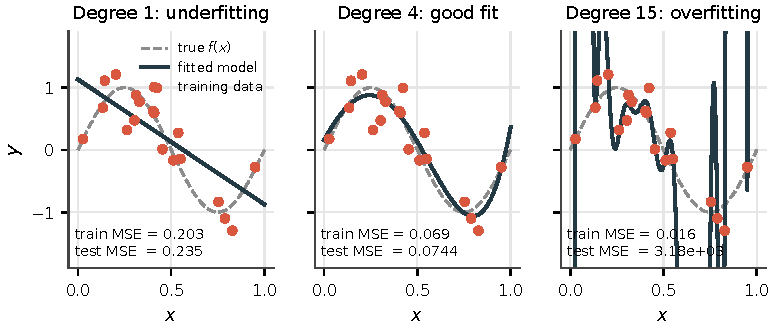
\includegraphics[width=\textwidth]{ch01/polyfits}
\caption{Underfitting and overfitting. Polynomials of degree 1, 4 and 15 fitted to the same
20 noisy observations of $\sin(2\pi x)$. The test error is computed on 5000 new points drawn
from the same range.}
\label{fig:polyfits}
\end{figure}

To see the decomposition at work, \cref{fig:biasvariance} repeats the experiment 500 times
with the same 40 input positions and fresh noise each time, and estimates each term of
\cref{eq:biasvariance}. As the degree grows, the bias drops quickly (from 0.54 for a
constant model to practically zero from degree~5 on), while the variance grows steadily
(from 0.002 to 0.061). The expected test error, which is their sum plus the noise, is
U-shaped, with its minimum at degree~3. The training error, in contrast, keeps decreasing:
it is blind to overfitting.

\begin{figure}[htbp]
\centering
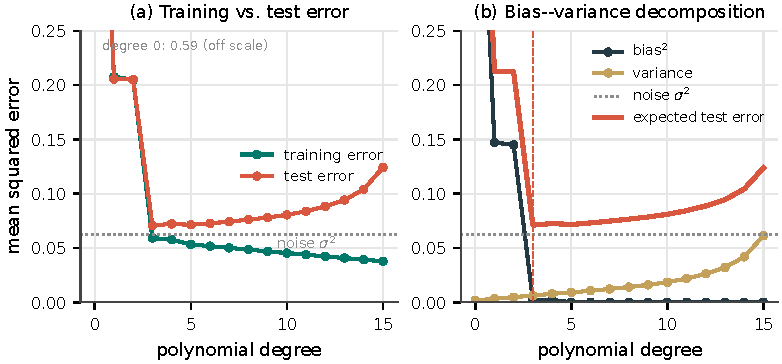
\includegraphics[width=\textwidth]{ch01/bias_variance}
\caption{(a) Training error decreases monotonically with model complexity, while test error
first decreases and then increases. (b) Bias--variance decomposition estimated by simulation
(500 training sets); the dashed line marks the complexity with the lowest expected error.}
\label{fig:biasvariance}
\end{figure}

For the 0--1 loss of classification the decomposition is not additive in the same simple way
\citep{domingos2000unified}, but the intuition carries over: flexible models have low bias and
high variance, rigid models the opposite \citep{geman1992neural}.

\subsection{Complexity in practice: the \texorpdfstring{$k$}{k}-nearest neighbours example}

The complexity of a model is controlled by its hyperparameters: the degree of a polynomial,
the depth of a tree, the strength of a regularisation term, the number of boosting\index{boosting}
iterations, or the number of neighbours $k$ in $k$-NN. \Cref{fig:knn} shows $k$-NN on a
two-moons problem. With $k=1$ every training point is classified correctly (training accuracy\index{accuracy}
1.00) but the frontier is jagged and the test accuracy is only 0.88; with $k=150$ the frontier
is almost a straight line and both accuracies are low (0.82 and 0.83); $k=15$ is a good
compromise (0.94 and 0.92). Choosing a hyperparameter is choosing a point on the bias--variance\index{bias--variance trade-off}
trade-off, and this choice requires data that are not used for training
(\cref{sec:protocols}).

\begin{figure}[htbp]
\centering
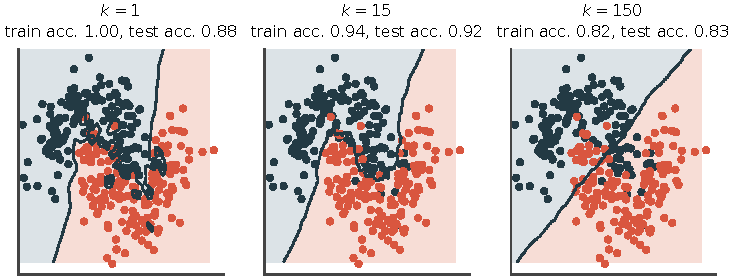
\includegraphics[width=\textwidth]{ch01/knn_boundaries}
\caption{Decision regions of $k$-NN on 300 training examples for three values of $k$. Small
$k$ means high variance (overfitting); large $k$ means high bias (underfitting).}
\label{fig:knn}
\end{figure}

\subsection{Learning curves}

A \emph{learning curve\index{learning curve|textbf}} plots the training and validation performance as a function of the
size of the training set (\cref{fig:learningcurves}). It is a simple and powerful diagnostic:
\begin{itemize}
  \item \emph{high bias}: both curves converge quickly to a similar, unsatisfactory value
        (logistic regression on the two moons, about 0.86). More data will not help; we need
        a more flexible model or better features;
  \item \emph{high variance}: there is a persistent gap between the training curve (1.00 for
        an unpruned tree) and the validation curve (0.88). More data, regularisation or
        ensembles\index{ensemble} (Unit~2) will help;
  \item a good compromise shows both curves close and high ($k$-NN with $k=25$: 0.92 and 0.91).
\end{itemize}

\begin{figure}[htbp]
\centering
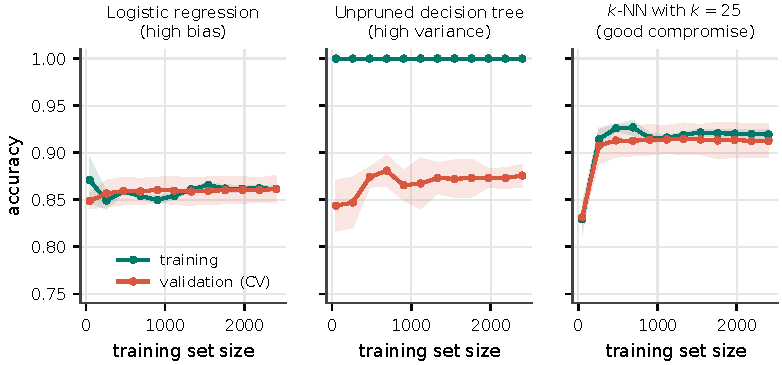
\includegraphics[width=\textwidth]{ch01/learning_curves}
\caption{Learning curves (mean and standard deviation over 5 folds) for three models on the
two-moons problem with 3000 examples.}
\label{fig:learningcurves}
\end{figure}

\begin{further}
The U-shaped curve of \cref{fig:biasvariance} is not the whole story for heavily
over-parameterised models such as deep neural networks. \citet{belkin2019reconciling}
documented a \emph{double descent}: beyond the point where the model can interpolate the
training data, the test error may decrease again as the number of parameters keeps growing.
For the models used in most tabular data science problems, the classical picture remains a
reliable guide.
\end{further}

% ---------------------------------------------------------------------
\section{Estimating performance: evaluation protocols}\label{sec:protocols}

The golden rule of evaluation is simple to state and easy to break: \emph{the performance of
a model must be estimated on data that played no role in building it}, and ``building''
includes preprocessing, feature selection, hyperparameter tuning\index{hyperparameter optimisation} and model selection.

\subsection{Training, validation and test data}

It is useful to separate two activities \citep[Chapter~7]{hastie2009elements}:
\emph{model selection}, which chooses among models or hyperparameters, and
\emph{model assessment}, which estimates the performance of the final choice. With enough
data, the cleanest approach uses three disjoint sets: a \emph{training set\index{training set|textbf}} to fit the
models, a \emph{validation set\index{validation set|textbf}} to choose among them, and a \emph{test set\index{test set|textbf}}, used once, to
assess the chosen model. If the test set is used repeatedly to take decisions, it silently
becomes a validation set and its estimates become optimistic; leaderboards of public
competitions show this effect regularly.

\subsection{Hold-out estimation}

The simplest protocol randomly splits the data into a training and a test set, typically
with 20--30\% of the data for testing. In classification the split should be
\emph{stratified\index{cross-validation!stratified|textbf}}, so that both parts keep the class proportions. The hold-out\index{hold-out} estimate is
cheap but has two drawbacks: the model is trained on less data than available, and the
estimate has high variance, because it depends on a single test sample. If a classifier with
true accuracy 0.85 is tested on 200 examples, the number of correct predictions is binomial,
the standard error of the accuracy is $\sqrt{0.85\cdot0.15/200}\approx0.025$, and an
approximate 95\% interval spans about $\pm0.05$. Differences of one or two points between
models tested this way mean very little (\cref{sec:stats}).

\subsection{Cross-validation}

In \emph{$k$-fold cross-validation\index{cross-validation|textbf}} (CV) the data are partitioned into $k$ folds
$F_1,\dots,F_k$ of similar size. Each fold is used once as test set while the model is
trained on the remaining $k-1$ folds (\cref{fig:cvschemes}a), and the estimate pools all the
test predictions:
\begin{equation}
  \widehat{R}_{\text{CV}}=\frac1n\sum_{j=1}^{k}\sum_{i\in F_j}\ell\bigl(y_i,h^{(-j)}(x_i)\bigr),
\end{equation}
where $h^{(-j)}$ is the model trained without fold $F_j$. Every example is used for testing
exactly once, and every model is trained on a fraction $(k-1)/k$ of the data. Some practical
points:
\begin{itemize}
  \item values of $k=5$ or $k=10$, with stratification, are a good compromise between bias
        and variance \citep{kohavi1995study};
  \item \emph{leave-one-out} CV ($k=n$) is almost unbiased but expensive and has high
        variance; \emph{repeated} CV, with several random partitions, reduces the variance
        due to the particular partition;
  \item CV estimates the performance of the \emph{learning procedure} when trained on
        $(k-1)n/k$ examples, not of a particular model. After CV, the final model is retrained
        on all the data, so the estimate is slightly pessimistic;
  \item the fold estimates are not independent (the training sets overlap), and there is no
        unbiased estimator of the variance of the CV estimate \citep{bengio2004no}. This has
        consequences for statistical tests (\cref{sec:stats}). \citet{arlot2010survey} review
        the theory.
\end{itemize}

\begin{figure}[htbp]
\centering
\begin{subfigure}[b]{0.49\textwidth}
\centering
\begin{tikzpicture}[x=9.5mm,y=5.5mm,font=\scriptsize\sffamily]
  \foreach \c in {1,...,5} \node at (\c-0.5,0.55) {Fold \c};
  \foreach \r in {1,...,5}{
    \node[anchor=east] at (-0.1,-\r+0.5) {Iteration \r};
    \foreach \c in {1,...,5}{
      \ifnum\c=\r
        \filldraw[fill=edmcoral!85,draw=white,thick] (\c-1,-\r) rectangle (\c,-\r+1);
      \else
        \filldraw[fill=edmnavy!18,draw=white,thick] (\c-1,-\r) rectangle (\c,-\r+1);
      \fi
    }
  }
\end{tikzpicture}
\caption{5-fold cross-validation}
\end{subfigure}\hfill
\begin{subfigure}[b]{0.49\textwidth}
\centering
\begin{tikzpicture}[x=4.4mm,y=5.5mm,font=\scriptsize\sffamily]
  \foreach \r in {1,...,4}{
    \node[anchor=east] at (-0.2,-\r+0.5) {Split \r};
    \pgfmathtruncatemacro{\ntr}{4+2*(\r-1)}
    \pgfmathtruncatemacro{\nte}{\ntr+2}
    \foreach \t in {0,...,11}{
      \ifnum\t<\ntr
        \filldraw[fill=edmnavy!18,draw=white,thick] (\t,-\r) rectangle (\t+1,-\r+1);
      \else\ifnum\t<\nte
        \filldraw[fill=edmcoral!85,draw=white,thick] (\t,-\r) rectangle (\t+1,-\r+1);
      \else
        \filldraw[fill=black!6,draw=white,thick] (\t,-\r) rectangle (\t+1,-\r+1);
      \fi\fi
    }
  }
  \draw[-{Stealth},thick,edmnavy] (0,-4.5) -- (12.4,-4.5) node[right] {time};
\end{tikzpicture}
\caption{Forward chaining for time series}
\end{subfigure}
\caption{Two evaluation schemes. Light blue: training data; red: test data; grey: data not
used in that split. In (b) the model is always tested on data that come after the training
period, as it will be in deployment (compare with \cref{lst:timeseries}).}
\label{fig:cvschemes}
\end{figure}

\subsection{The bootstrap}

A bootstrap\index{bootstrap} sample is obtained by drawing $n$ examples \emph{with replacement} from the data
set. The probability that a given example is never drawn is $(1-1/n)^n\approx e^{-1}\approx
0.368$, so each bootstrap sample contains about 63.2\% of the distinct examples, and the
remaining \emph{out-of-bag\index{out-of-bag estimate|textbf}} (OOB) examples can be used for testing. Repeating the process $B$
times and averaging the OOB errors gives a pessimistic estimate (each model sees only 63.2\%
of the distinct examples); the \emph{.632 estimator} corrects it by mixing it with the
optimistic training error,
\begin{equation}
  \widehat R_{.632}=0.368\,\widehat R_{\text{train}}+0.632\,\widehat R_{\text{OOB}},
\end{equation}
and the \emph{.632+} variant further corrects the case of strongly overfitting models
\citep{efron1997improvements}. The bootstrap is also the standard tool to build confidence
intervals\index{confidence interval} for any metric (\cref{sec:stats}), and the OOB idea is used by random forests
(Unit~2).

\subsection{Model selection and nested cross-validation}

Hyperparameters are usually tuned by evaluating many candidate configurations with
cross-validation and keeping the best one. The CV score of the winner, however, is
optimistically biased: when many candidates are compared on the same data, the best one is
partly the luckiest one \citep{varma2006bias,cawley2010over}. To estimate the performance of
the whole procedure (``tune with grid search\index{grid search}, then train''), the tuning must itself be
evaluated inside an outer CV loop. This is \emph{nested cross-validation\index{cross-validation!nested|textbf}\index{cross-validation|textbf}}
(\cref{alg:nestedcv}).

\begin{algorithm}[htbp]
\caption{Nested cross-validation}\label{alg:nestedcv}
\begin{algorithmic}[1]
\Require data $D$; learning procedure $\mathcal A_\theta$ with hyperparameters
         $\theta\in\Theta$; numbers of outer and inner folds $K$ and $J$
\State split $D$ into outer folds $F_1,\dots,F_K$
\For{$k=1,\dots,K$}
  \State $D_{\text{tr}}\gets D\setminus F_k$
  \For{each $\theta\in\Theta$} \Comment{inner loop: model selection}
    \State $\text{score}(\theta)\gets$ $J$-fold CV estimate of $\mathcal A_\theta$ on $D_{\text{tr}}$
  \EndFor
  \State $\theta_k^\star\gets\argmax_\theta\ \text{score}(\theta)$
  \State $h_k\gets\mathcal A_{\theta_k^\star}(D_{\text{tr}})$ \Comment{refit on the outer training data}
  \State $e_k\gets$ performance of $h_k$ on $F_k$ \Comment{outer loop: assessment}
\EndFor
\State \Return $\frac1K\sum_{k}e_k$ \Comment{estimate for the \emph{whole} tuning procedure}
\end{algorithmic}
\end{algorithm}

\Cref{lst:nested} tunes an SVM over 30 hyperparameter combinations on a small, noisy problem.
The inner-CV AUC of the selected configuration is 0.782, but the honest nested estimate is
0.746: an optimism of almost four points of AUC, larger than many of the differences between
models reported in practice. Note that nested CV evaluates the tuning \emph{procedure}; the
model finally deployed is obtained by running that procedure on all the data.

\begin{pylisting}[label={lst:nested}]{Optimistic bias of the best inner-CV score and nested cross-validation}
from sklearn.datasets import make_classification
from sklearn.model_selection import GridSearchCV, StratifiedKFold, cross_val_score
from sklearn.pipeline import make_pipeline
from sklearn.preprocessing import StandardScaler
from sklearn.svm import SVC

# A small, noisy problem: 150 examples, 40 features (only 4 informative)
X, y = make_classification(n_samples=150, n_features=40, n_informative=4,
                           flip_y=0.15, class_sep=0.8, random_state=2)
inner = StratifiedKFold(5, shuffle=True, random_state=1)
outer = StratifiedKFold(5, shuffle=True, random_state=2)
grid = {"svc__C": [0.01, 0.1, 1, 10, 100, 1000],
        "svc__gamma": [1e-4, 1e-3, 1e-2, 1e-1, 1]}          # 30 candidate models
search = GridSearchCV(make_pipeline(StandardScaler(), SVC()), grid,
                      cv=inner, scoring="roc_auc")

search.fit(X, y)                     # model selection using all the data
print(f"Selected: {search.best_params_}")
print(f"Inner-CV AUC of the selected model (optimistic): {search.best_score_:.4f}")
# Nested CV: the WHOLE tuning procedure is repeated inside each outer fold
nested = cross_val_score(search, X, y, cv=outer, scoring="roc_auc")
print(f"Nested CV AUC (honest): {nested.mean():.4f} +/- {nested.std():.4f}")
\end{pylisting}
\begin{pyoutput}
Selected: {'svc__C': 1, 'svc__gamma': 0.01}
Inner-CV AUC of the selected model (optimistic): 0.7822
Nested CV AUC (honest): 0.7458 +/- 0.0257
\end{pyoutput}

\subsection{Dependent data: groups and time}

Random splits assume that examples are independent. When they are not, random CV is
optimistic, because information leaks between related training and test examples:
\begin{itemize}
  \item \emph{grouped data}: several examples come from the same patient, customer, device
        or session. All the examples of a group must fall on the same side of each split
        (\code{GroupKFold} in scikit-learn); otherwise the model is tested on ``people'' it
        has already seen;
  \item \emph{temporal data}: the model will always predict the future from the past, so it
        must be evaluated the same way, training on an initial period and testing on the
        following one (\emph{forward chaining} or \emph{rolling-origin} evaluation,
        \cref{fig:cvschemes}b and \cref{lst:timeseries}). A gap between training and test
        periods avoids leakage\index{data leakage} through autocorrelation. \citet{bergmeir2012use} discuss when
        standard CV is still acceptable for time series;
  \item \emph{spatial data}: nearby locations are similar, and blocked spatial CV is
        needed \citep{roberts2017cross}.
\end{itemize}

\begin{pylisting}[label={lst:timeseries}]{Forward-chaining splits for 12 consecutive time steps}
import numpy as np
from sklearn.model_selection import TimeSeriesSplit

X = np.arange(12).reshape(-1, 1)          # 12 consecutive time steps
for k, (tr, te) in enumerate(TimeSeriesSplit(n_splits=4, test_size=2).split(X), 1):
    print(f"fold {k}: train={tr.tolist()}  test={te.tolist()}")
\end{pylisting}
\begin{pyoutput}
fold 1: train=[0, 1, 2, 3]  test=[4, 5]
fold 2: train=[0, 1, 2, 3, 4, 5]  test=[6, 7]
fold 3: train=[0, 1, 2, 3, 4, 5, 6, 7]  test=[8, 9]
fold 4: train=[0, 1, 2, 3, 4, 5, 6, 7, 8, 9]  test=[10, 11]
\end{pyoutput}

\subsection{Data leakage}

\emph{Data leakage\index{data leakage|textbf}} is the use, during training or evaluation, of information that would not
be available when the model is used in practice \citep{kaufman2012leakage}. It is the most
common cause of results that look too good to be true. Typical forms are:
\begin{itemize}
  \item \emph{target leakage}: features that are consequences of the target or are recorded
        after the event (the number of days in hospital to predict hospital admission, or a
        late-payment fee to predict default);
  \item \emph{train--test contamination\index{contamination of benchmarks|textbf}}: preprocessing steps (scaling, imputation, feature
        selection, resampling, target encoding) fitted on the whole data set before
        splitting it;
  \item \emph{temporal leakage}: random splits of time-ordered data, or features computed
        with future information;
  \item \emph{duplicates}: identical or near-identical examples (the same patient, the same
        product photographed twice, augmented copies) on both sides of a split.
\end{itemize}
\Cref{lst:leakage} reproduces a classic experiment \citep[Section~7.10.2]{hastie2009elements}.
With 5000 pure-noise features and random labels, any honest estimate of accuracy must be
close to 0.5. Selecting the 20 features most correlated with the labels \emph{before}
cross-validation produces an estimated accuracy of 0.87; doing the selection inside each fold
gives the correct 0.50. \citet{kapoor2023leakage} found leakage of this kind in hundreds of
published studies across many scientific fields.

\begin{pylisting}[label={lst:leakage}]{Feature selection outside versus inside cross-validation}
import numpy as np
from sklearn.feature_selection import SelectKBest, f_classif
from sklearn.linear_model import LogisticRegression
from sklearn.model_selection import StratifiedKFold, cross_val_score
from sklearn.pipeline import make_pipeline

rng = np.random.default_rng(0)
X = rng.normal(size=(100, 5000))    # 5000 pure-noise features
y = rng.integers(0, 2, size=100)    # random labels: true accuracy is 0.5
cv = StratifiedKFold(n_splits=5, shuffle=True, random_state=0)
clf = LogisticRegression(max_iter=1000)

# WRONG: the features are selected looking at ALL the labels, then we do CV
X_sel = SelectKBest(f_classif, k=20).fit_transform(X, y)
wrong = cross_val_score(clf, X_sel, y, cv=cv)

# RIGHT: selection is part of the model, so it is refitted inside each fold
right = cross_val_score(make_pipeline(SelectKBest(f_classif, k=20), clf), X, y, cv=cv)
print(f"Wrong CV accuracy: {wrong.mean():.2f}")
print(f"Right CV accuracy: {right.mean():.2f}")
\end{pylisting}
\begin{pyoutput}
Wrong CV accuracy: 0.87
Right CV accuracy: 0.50
\end{pyoutput}

\begin{pitfall}
Any step that looks at the data (including the labels) is part of the model. Put scaling,
imputation, feature selection, resampling and encoders inside a \code{Pipeline}, and evaluate
the pipeline, never a model fitted on preprocessed data.
\end{pitfall}

% ---------------------------------------------------------------------
\section{Evaluating crisp classifiers}\label{sec:crisp}

A \emph{crisp} classifier outputs a class label, $h:\mathcal X\to\{1,\dots,c\}$. Scoring and
probabilistic classifiers, which output degrees of confidence, are treated in
\cref{sec:roc,sec:scoring}.

\subsection{Error and accuracy}

Given a set $S$ of $n$ examples, the \emph{error} of $h$ is the proportion of misclassified
examples,
\begin{equation}
  \operatorname{error}_S(h)=\frac1n\sum_{x\in S}\delta\bigl(f(x),h(x)\bigr),
  \qquad
  \delta(a,b)=\begin{cases}0 & \text{if } a=b,\\ 1 & \text{otherwise,}\end{cases}
\end{equation}
and the \emph{accuracy\index{accuracy|textbf}} is $1-\operatorname{error}_S(h)$.

\begin{example}{A purchase prediction model}{purchase}
A shop predicts whether each of ten customers will buy a product (positive class
\emph{buy}). The predictions and the actual behaviour are:
\begin{center}\small
\begin{tabular}{@{}cccc|cccc@{}}
\toprule
Customer & Predicted & Actual & Error & Customer & Predicted & Actual & Error\\
\midrule
1 & buy    & buy    & no  & 6  & no buy & buy    & yes\\
2 & no buy & buy    & yes & 7  & no buy & no buy & no\\
3 & buy    & no buy & yes & 8  & buy    & buy    & no\\
4 & buy    & buy    & no  & 9  & buy    & buy    & no\\
5 & no buy & no buy & no  & 10 & no buy & no buy & no\\
\bottomrule
\end{tabular}
\end{center}
Three predictions are wrong, so the error is $3/10=0.3$ (30\%) and the accuracy $7/10=0.7$
(70\%). We will use this example throughout the section.
\end{example}

\subsection{The confusion matrix}

Accuracy hides \emph{which} errors are made. The \emph{confusion matrix\index{confusion matrix|textbf}} counts the examples
for every combination of predicted and actual class. In this book we follow the convention
of \citet{fawcett2006introduction}: rows correspond to the \emph{predicted} class and columns
to the \emph{actual} class. In binary problems, one class is called \emph{positive} (usually
the class of interest: the disease, the fraud, the purchase) and the other \emph{negative},
which gives the four cells of \cref{tab:confusion}. We write $P=\TP+\FN$ and $N=\FP+\TN$ for
the number of actual positives and negatives.

\begin{table}[htbp]
\centering\small
\caption{Binary confusion matrix (left) and the matrix of the purchase example of
\cref{ex:purchase} (right), with \emph{buy} as the positive class.}\label{tab:confusion}
\begin{tabular}{@{}llcc@{}}
\toprule
& & \multicolumn{2}{c}{Actual class}\\
\cmidrule(l){3-4}
& & Positive & Negative\\
\midrule
\multirow{2}{*}{Predicted} & Positive & $\TP$ & $\FP$\\
                           & Negative & $\FN$ & $\TN$\\
\midrule
& Total & $P$ & $N$\\
\bottomrule
\end{tabular}\qquad
\begin{tabular}{@{}llcc@{}}
\toprule
& & \multicolumn{2}{c}{Actual class}\\
\cmidrule(l){3-4}
& & buy & no buy\\
\midrule
\multirow{2}{*}{Predicted} & buy    & 4 & 1\\
                           & no buy & 2 & 3\\
\midrule
& Total & 6 & 4\\
\bottomrule
\end{tabular}
\end{table}

\begin{pitfall}
Conventions differ. Many textbooks and scikit-learn's \code{confusion_matrix} put the
\emph{actual} class in the rows and the \emph{predicted} class in the columns, and sort the
labels, so that for 0/1 labels the negative class comes first:
\code{tn, fp, fn, tp = confusion_matrix(y, y_pred).ravel()}. Transposing the matrix swaps
$\FP$ and $\FN$, and therefore swaps sensitivity\index{sensitivity} and precision. Always check the convention
before reading a confusion matrix.
\end{pitfall}

\subsection{Metrics derived from the confusion matrix}

\Cref{tab:metrics} collects the most common metrics, with their values for the purchase
example ($\TP=4$, $\FN=2$, $\FP=1$, $\TN=3$), and \cref{lst:confusion} computes them with
scikit-learn.

\begin{table}[htbp]
\centering\small
\caption{Metrics computed from a binary confusion matrix and their values for the purchase
example.}\label{tab:metrics}
\begin{tabularx}{\textwidth}{@{}>{\raggedright\arraybackslash}p{3.3cm}>{\raggedright\arraybackslash}X>{\raggedright\arraybackslash}p{4.6cm}r@{}}
\toprule
Metric & Also known as & Definition & Example\\
\midrule
True positive rate & sensitivity, recall, hit rate & $\TPR=\TP/P=1-\FNR$ & $4/6=0.667$\\
True negative rate & specificity & $\TNR=\TN/N=1-\FPR$ & $3/4=0.750$\\
False positive rate & fall-out, false alarm rate & $\FPR=\FP/N$ & $1/4=0.250$\\
False negative rate & miss rate & $\FNR=\FN/P$ & $2/6=0.333$\\
Positive predictive value & precision & $\PPV=\TP/(\TP+\FP)$ & $4/5=0.800$\\
Negative predictive value & & $\NPV=\TN/(\TN+\FN)$ & $3/5=0.600$\\
Accuracy & $1-$error & $(\TP+\TN)/(P+N)$ & $7/10=0.700$\\
Balanced accuracy & macro-averaged accuracy & $(\TPR+\TNR)/2$ & $0.708$\\
G-mean & & $\sqrt{\TPR\cdot\TNR}$ & $0.707$\\
$F_1$ score & F-measure & $2\,\PPV\cdot\TPR/(\PPV+\TPR)$ $=2\TP/(2\TP+\FP+\FN)$ & $8/11=0.727$\\
$F_\beta$ score & & $(1+\beta^2)\,\PPV\cdot\TPR/(\beta^2\PPV+\TPR)$ & \\
Matthews correlation coefficient & MCC, $\phi$ coefficient & see \cref{eq:mcc} & $0.408$\\
\bottomrule
\end{tabularx}
\end{table}

The Matthews correlation coefficient\index{Matthews correlation coefficient}, which needs more room than the table allows, is
\begin{equation}\label{eq:mcc}
  \mathrm{MCC}=\frac{\TP\cdot\TN-\FP\cdot\FN}{\sqrt{(\TP+\FP)(\TP+\FN)(\TN+\FP)(\TN+\FN)}}
  =\frac{4\cdot3-1\cdot2}{\sqrt{5\cdot6\cdot4\cdot5}}=0.408 .
\end{equation}
When a row or a column of the confusion matrix\index{confusion matrix} is empty (for instance, a classifier that always
predicts negative), the denominator is zero and the MCC is undefined; \textsf{scikit-learn} returns 0 by
convention.

\begin{pylisting}[label={lst:confusion}]{Confusion matrix and derived metrics for the purchase example}
import numpy as np
from sklearn.metrics import (confusion_matrix, accuracy_score, recall_score,
                             precision_score, f1_score, balanced_accuracy_score,
                             matthews_corrcoef, cohen_kappa_score)

# Purchase example: 1 = "buy" (positive class), 0 = "no buy"
y_true = np.array([1, 1, 0, 1, 0, 1, 0, 1, 1, 0])
y_pred = np.array([1, 0, 1, 1, 0, 0, 0, 1, 1, 0])

# scikit-learn convention: rows = ACTUAL class, columns = PREDICTED class
tn, fp, fn, tp = confusion_matrix(y_true, y_pred).ravel()
print(f"TP={tp} FN={fn} FP={fp} TN={tn}")
print(f"accuracy          {accuracy_score(y_true, y_pred):.4f}")
print(f"sensitivity (TPR) {recall_score(y_true, y_pred):.4f}")
print(f"specificity (TNR) {recall_score(y_true, y_pred, pos_label=0):.4f}")
print(f"precision (PPV)   {precision_score(y_true, y_pred):.4f}")
print(f"F1 score          {f1_score(y_true, y_pred):.4f}")
print(f"balanced accuracy {balanced_accuracy_score(y_true, y_pred):.4f}")
print(f"MCC               {matthews_corrcoef(y_true, y_pred):.4f}")
print(f"Cohen's kappa     {cohen_kappa_score(y_true, y_pred):.4f}")
\end{pylisting}
\begin{pyoutput}
TP=4 FN=2 FP=1 TN=3
accuracy          0.7000
sensitivity (TPR) 0.6667
specificity (TNR) 0.7500
precision (PPV)   0.8000
F1 score          0.7273
balanced accuracy 0.7083
MCC               0.4082
Cohen's kappa     0.4000
\end{pyoutput}

A few remarks help to choose among them:
\begin{itemize}
  \item $\TPR$, $\TNR$, $\FPR$ and $\FNR$ are computed within a single column of the matrix,
        that is, within one actual class. They, and their combinations (balanced accuracy\index{balanced accuracy},
        G-mean), \emph{do not depend on the class distribution} of the test set, as long as the
        class-conditional distributions stay the same (label shift\index{label shift}; \cref{ch:monitoring} discusses other shifts). Precision,
        NPV\index{predictive value!negative}, accuracy, $F_1$, MCC and kappa mix both columns and \emph{do} depend on it:
        comparisons across different class mixtures confound model behaviour with prevalence\index{prevalence}
        unless the operating context is accounted for;
  \item sensitivity\index{sensitivity} and specificity\index{specificity}, or precision and recall, always come in pairs: a model
        can trivially maximise one at the expense of the other. Balanced accuracy, the
        G-mean and $F_\beta$ summarise each pair; $\beta>1$ weighs recall more than
        precision \citep{vanrijsbergen1979information};
  \item $F_1$ ignores the true negatives, which is appropriate in information retrieval,
        where negatives are innumerable and uninteresting, but it also means that $F_1$
        changes if we swap the roles of the two classes;
  \item the MCC uses the four cells, is symmetric in the classes, ranges from $-1$ to $1$ and
        is 0 for random predictions \citep{matthews1975comparison}. It is a good single-number
        summary for imbalanced\index{class imbalance} binary problems \citep{chicco2020advantages}. The G-mean
        was proposed for imbalanced problems by \citet{kubat1997addressing}, and
        \citet{brodersen2010balanced} discuss balanced accuracy.
        \citet{sokolova2009systematic} analyse the properties of many more metrics.
\end{itemize}

\subsection{Agreement beyond chance: Cohen's kappa}

Accuracy does not take into account that some agreement between predictions and actual
classes happens by chance. \emph{Cohen's kappa\index{Cohen's kappa|textbf}} \citep{cohen1960coefficient} corrects for it:
\begin{equation}
  \kappa=\frac{p_o-p_e}{1-p_e},
  \qquad
  p_e=\sum_{j=1}^{c}\frac{n_{j\cdot}}{n}\,\frac{n_{\cdot j}}{n},
\end{equation}
where $p_o$ is the observed agreement (the accuracy) and $p_e$ the agreement expected if
predictions and actual classes were independent with the same marginals ($n_{j\cdot}$ and
$n_{\cdot j}$ are the row and column totals of class $j$). In the purchase example the model
predicts \emph{buy} for 5 customers and 6 actually buy, so
$p_e=0.5\cdot0.6+0.5\cdot0.4=0.5$ and $\kappa=(0.7-0.5)/(1-0.5)=0.4$. Kappa is 1 for complete
agreement, 0 for agreement at chance level, and negative for agreement worse than chance.
\citet{landis1977measurement} proposed a widely used (and admittedly arbitrary) scale: values
of 0.21--0.40 indicate fair agreement, 0.41--0.60 moderate, 0.61--0.80 substantial and above
0.80 almost perfect agreement.

Kappa was designed to measure the agreement between two \emph{annotators}, and this is still
one of its main uses in data science: before training a model on manually labelled data,
measuring the agreement between two labellers tells us how reliable the labels are, and
gives an informal upper bound on the performance we can expect from the model.

\subsection{Prevalence and predictive values}

The probability that a positive prediction is correct depends not only on the classifier but
also on the prevalence\index{prevalence} $\pi_+$ of the positive class. By Bayes' theorem,
\begin{equation}\label{eq:ppv}
  \PPV=\frac{\TPR\cdot\pi_+}{\TPR\cdot\pi_++\FPR\cdot(1-\pi_+)},
  \qquad
  \NPV=\frac{\TNR\cdot(1-\pi_+)}{\TNR\cdot(1-\pi_+)+\FNR\cdot\pi_+}.
\end{equation}
A diagnostic test with sensitivity\index{sensitivity} 0.95 and specificity\index{specificity} 0.98 sounds excellent, but if the
disease affects 1\% of the population, $\PPV=0.0095/(0.0095+0.0198)=0.324$: two out of three
positive results are false alarms. \Cref{fig:prevalence} shows how the predictive values of two
tests change with prevalence. Test~B, with a much lower sensitivity (0.60) but higher
specificity (0.995), has a \emph{higher} PPV\index{predictive value!positive} at low prevalence (0.548 at 1\%), because when
positives are rare it is the specificity that controls the number of false alarms.

\begin{figure}[htbp]
\centering
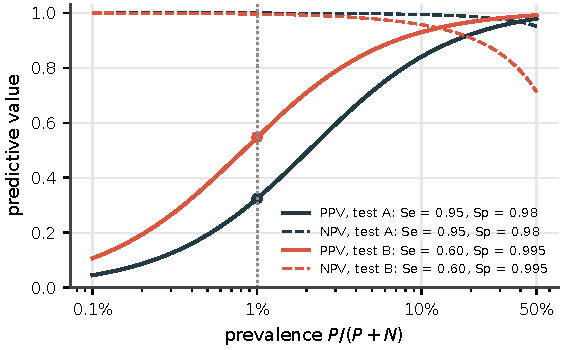
\includegraphics[width=0.72\textwidth]{ch01/prevalence_ppv}
\caption{Positive (solid) and negative (dashed) predictive values as a function of prevalence
for two tests. The dots mark the PPV at a prevalence of 1\%.}
\label{fig:prevalence}
\end{figure}

\begin{example}{What is the sensitivity of a COVID-19 test?}{covid}
During the COVID-19 pandemic, rapid antigen tests were criticised because, compared with PCR,
they missed a substantial fraction of infections. \citet{mina2020rethinking} argued that this
comparison used the wrong reference for the purpose of \emph{containment}. PCR detects viral
RNA long before and long after a person is infectious, whereas antigen tests detect the high
viral loads typical of the infectious period. If the goal is to stop transmission, what
matters is the sensitivity for \emph{infectious} people, and also how often and how fast
results are obtained: a cheap test used frequently, with immediate results, can prevent more
transmission than a very sensitive test whose result arrives two days later.

The lesson goes beyond medicine: a metric is only meaningful with respect to a reference
(what counts as a ``true'' positive) and to the context in which the model is deployed.
\end{example}

\subsection{Multiclass problems}

With $c$ classes the confusion matrix\index{confusion matrix} $M$ is $c\times c$, with $M_{jk}$ the number of examples
predicted as class $j$ whose actual class is $k$. Per-class metrics are obtained by treating
each class as positive and the rest as negative (\emph{one-versus-all\index{one-versus-all|textbf}}, OVA): for class $j$,
$\TP_j=M_{jj}$, $\FP_j=\sum_{k\neq j}M_{jk}$ (rest of the row) and $\FN_j=\sum_{k\neq j}M_{kj}$
(rest of the column). The per-class results are then averaged:
\begin{itemize}
  \item \emph{macro} average: plain mean over classes, which gives the same weight to every
        class and therefore emphasises small classes;
  \item \emph{weighted} average: mean weighted by the number of examples of each class, which
        reflects the class distribution of the test set;
  \item \emph{micro} average: the counts $\TP_j$, $\FP_j$, $\FN_j$ are pooled before
        computing the metric. In single-label problems micro precision, micro recall and
        micro $F_1$ all equal the accuracy.
\end{itemize}
Metrics defined only for two classes can also be extended with the \emph{one-versus-one\index{one-versus-one|textbf}}
(OVO) approach, which computes $c(c-1)/2$ results, one for each pair of classes.

\begin{example}{Three classes}{multiclass}
A classifier of animal pictures produces the following confusion matrix on 20 test images
(rows: predicted; columns: actual):
\begin{center}\small
\begin{tabular}{@{}lccc@{}}
\toprule
{\footnotesize pred.\,\textbackslash\,actual} & cat & dog & rabbit\\
\midrule
cat    & 8 & 1 & 0\\
dog    & 2 & 4 & 1\\
rabbit & 0 & 1 & 3\\
\bottomrule
\end{tabular}
\end{center}
For \emph{dog}: $\TP=4$, $\FP=2+1=3$ and $\FN=1+1=2$, so precision is $4/7=0.571$ and recall
$4/6=0.667$. \Cref{lst:multiclass} computes all the per-class and averaged values (note that
the matrix is written transposed in the code, following scikit-learn's convention). The
accuracy is 0.75; the macro-averaged\index{macro-average} $F_1$ (0.736) is lower than the weighted one (0.756)
because the worst class, \emph{dog}, counts as much as \emph{cat} in the macro average.
\end{example}

\begin{pylisting}[label={lst:multiclass}]{Per-class and averaged metrics for the three-class example}
import numpy as np
from sklearn.metrics import classification_report

cm = np.array([[8, 2, 0],      # rows: actual class (cat, dog, rabbit)
               [1, 4, 1],      # columns: predicted class
               [0, 1, 3]])
y_true = np.repeat(np.arange(3), cm.sum(axis=1))
y_pred = np.concatenate([np.repeat(np.arange(3), row) for row in cm])
print(classification_report(y_true, y_pred, digits=3,
                            target_names=["cat", "dog", "rabbit"]))
\end{pylisting}
\begin{pyoutput}
              precision    recall  f1-score   support

         cat      0.889     0.800     0.842        10
         dog      0.571     0.667     0.615         6
      rabbit      0.750     0.750     0.750         4

    accuracy                          0.750        20
   macro avg      0.737     0.739     0.736        20
weighted avg      0.766     0.750     0.756        20
\end{pyoutput}

% ---------------------------------------------------------------------
\section{ROC analysis}\label{sec:roc}

\subsection{Origins: signal detection}

Receiver Operating Characteristic\index{ROC analysis} (ROC) analysis originated in signal detection theory,
developed to analyse radar signals during the Second World War and later used extensively in
psychophysics and medical diagnosis \citep{green1966signal}. The problem is to decide whether
a signal is present in a noisy observation. If the observations follow one distribution when
there is only noise and another when signal is present, any decision rule\index{decision rules} of the form ``say
\emph{signal} if the observation exceeds a threshold $t$'' trades hits (true positives)
against false alarms (false positives), and the best threshold depends on the strength of the
signal, on the noise variance and on the hit or false alarm rate we are willing to accept
(\cref{fig:signal}). \citet{spackman1989signal} was one of the first to use ROC graphs to
evaluate machine learning algorithms.

\begin{figure}[htbp]
\centering
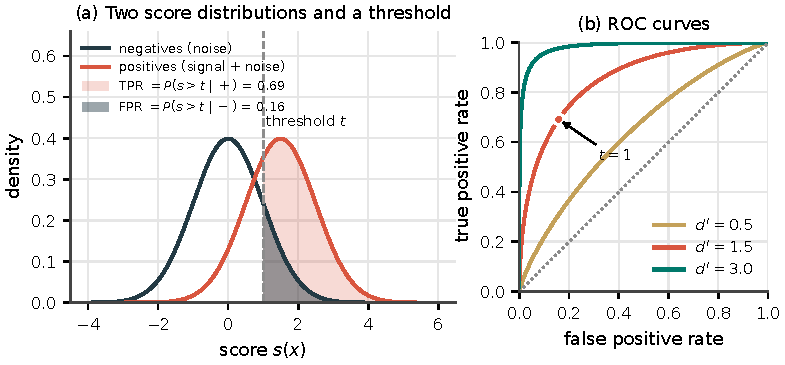
\includegraphics[width=\textwidth]{ch01/signal_detection}
\caption{(a) Scores of negatives $\mathcal N(0,1)$ and positives $\mathcal N(1.5,1)$; a threshold
$t=1$ gives $\TPR=0.69$ and $\FPR=0.16$. (b) Moving the threshold traces a ROC curve; the
curve depends on the separation $d'$ between the two distributions.}
\label{fig:signal}
\end{figure}

\subsection{The ROC space}

A crisp classifier is represented in the \emph{ROC space\index{ROC space|textbf}} by the point $(\FPR,\TPR)$. For
instance, a classifier with $\TP=3$, $\FN=1$, $\FP=3$ and $\TN=7$ has $\TPR=3/4=0.75$ and
$\FPR=3/10=0.30$, point A in \cref{fig:rocspace}. Some points are special:
\begin{itemize}
  \item $(0,0)$ is the classifier that always predicts negative (AlwaysNeg) and $(1,1)$ the one
        that always predicts positive (AlwaysPos);
  \item $(0,1)$ is the perfect classifier (``ROC heaven'') and $(1,0)$ the classifier that is
        always wrong (``ROC hell'');
  \item a classifier that predicts positive at random with probability $p$ lies at $(p,p)$:
        the diagonal contains all the random classifiers;
  \item a classifier below the diagonal is worse than random, but it contains useful
        information: inverting its predictions maps $(\FPR,\TPR)$ to $(1-\FPR,1-\TPR)$, a point
        above the diagonal (A$'$ becomes A in \cref{fig:rocspace}).
\end{itemize}
Since both coordinates are computed within one actual class, the position of a classifier in
ROC space does not depend on the class distribution or on the costs. This is what makes ROC
analysis\index{ROC analysis} useful when the deployment context is uncertain.

\begin{figure}[htbp]
\centering
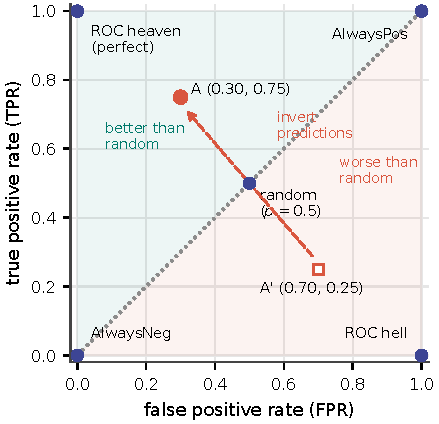
\includegraphics[width=0.58\textwidth]{ch01/roc_space}
\caption{The ROC space. Points above the diagonal are better than random; a classifier below
it can be improved by inverting its predictions.}
\label{fig:rocspace}
\end{figure}

\subsection{Iso-performance lines and the ROC convex hull}

Assume that correct predictions cost nothing and that a false negative and a false positive
cost $c_{\mathrm{FN}}$ and $c_{\mathrm{FP}}$. The expected cost\index{expected cost} per example of a classifier
at $(\FPR,\TPR)$ is
\begin{equation}\label{eq:rocost}
  \text{Cost}=\pi_+\,(1-\TPR)\,c_{\mathrm{FN}}+\pi_-\,\FPR\,c_{\mathrm{FP}}.
\end{equation}
All the classifiers with the same expected cost lie on a straight line
$\TPR=m\cdot\FPR+b$, an \emph{iso-performance line}, with slope
\begin{equation}\label{eq:isoslope}
  m=\frac{\pi_-\,c_{\mathrm{FP}}}{\pi_+\,c_{\mathrm{FN}}}=\frac{N}{P}\cdot\frac{c_{\mathrm{FP}}}{c_{\mathrm{FN}}}.
\end{equation}
For accuracy (equal costs) the slope is simply the class ratio $C=N/P$, and the lines are
called \emph{iso-accuracy\index{iso-accuracy line|textbf}\index{accuracy|textbf} lines} \citep{flach2003geometry}. Steep lines (many negatives or
expensive false positives) favour conservative classifiers close to $(0,0)$; flat lines
favour liberal classifiers close to $(1,1)$.

To find the best classifier for a given slope, move a line with that slope from the
upper-left corner towards the lower right until it touches a classifier. The classifiers that
can be touched first lie on the \emph{ROC convex hull\index{ROC convex hull|textbf}} (ROCCH) of the set of points, including
the trivial classifiers $(0,0)$ and $(1,1)$ \citep{provost2001robust}. Hence:
\begin{itemize}
  \item classifiers below the hull are never optimal, whatever the class distribution or the
        costs;
  \item each vertex of the hull is optimal for the range of slopes between the slopes of its
        two adjacent segments;
  \item any point on a segment of the hull can be achieved by choosing randomly, for each
        example, between the two classifiers at its ends.
\end{itemize}

\begin{example}{Choosing a classifier for each context}{rochull}
Five classifiers have been evaluated on the same test set:
\begin{center}\small
\begin{tabular}{@{}lccccc@{}}
\toprule
& CN2 & Ripper & C4.5 & NB & SVM\\
\midrule
FPR\index{false positive rate} & 0.05 & 0.10 & 0.16 & 0.28 & 0.60\\
TPR\index{true positive rate} & 0.50 & 0.60 & 0.80 & 0.70 & 0.95\\
\bottomrule
\end{tabular}
\end{center}
The convex hull is $(0,0)\to\text{CN2}\to\text{C4.5}\to\text{SVM}\to(1,1)$, with segment slopes
$10$, $2.73$, $0.34$ and $0.125$; Ripper and NB lie below it (\cref{fig:rochull}).
\begin{itemize}
  \item With balanced classes, $C=1$ lies between 2.73 and 0.34, so C4.5 is optimal, with
        accuracy $0.5\cdot0.80+0.5\cdot(1-0.16)=0.82$.
  \item With four times more positives than negatives, $C=1/4$ lies between 0.34 and 0.125:
        SVM is optimal, with accuracy $0.8\cdot0.95+0.2\cdot0.40=0.84$.
  \item With four times more negatives, $C=4$ lies between 10 and 2.73: CN2 is optimal, with
        accuracy $0.2\cdot0.50+0.8\cdot0.95=0.86$.
  \item AlwaysNeg is optimal when $C>10$, that is, when less than $1/11\approx9\%$ of the
        examples are positive; AlwaysPos is optimal when $C<0.125$, that is, when less than
        $1/9\approx11\%$ are negative.
\end{itemize}
No classifier is the best in all contexts, and two of them are the best in none.
\end{example}

\begin{figure}[htbp]
\centering
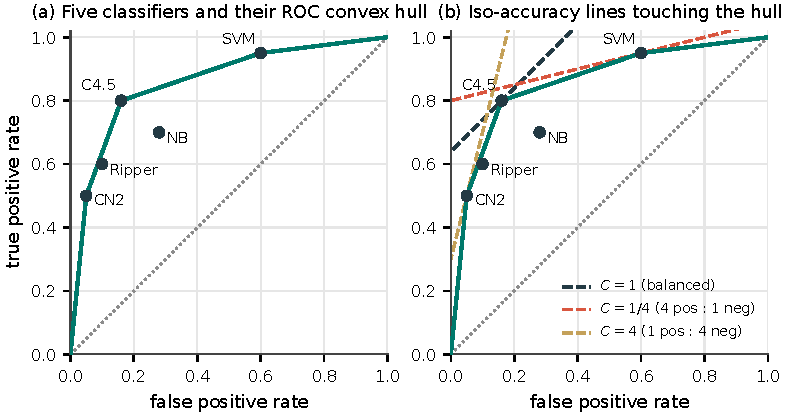
\includegraphics[width=\textwidth]{ch01/roc_hull}
\caption{(a) The ROC convex hull of the five classifiers of \cref{ex:rochull}. (b) The
iso-accuracy lines for three class ratios touch the hull at the optimal classifier for each
context.}
\label{fig:rochull}
\end{figure}

\subsection{Scoring classifiers and ROC curves}

Most classifiers can output a \emph{score} rather than a label: a scoring classifier\index{scoring classifier} assigns
to each example a real-valued score $s(x)$, with larger values indicating stronger evidence for the positive class,
such as a predicted positive-class probability or a signed decision margin. Ratios are useful in specific cases, such
as posterior odds or a likelihood ratio $P(x\mid+)/P(x\mid-)$ with a positive denominator; arbitrary class scores need
not admit such an interpretation (with scores $g(x)$ and $-g(x)$ for the two classes, the ratio is always $-1$). Any
strictly increasing transformation of $s(x)$ ranks the examples in the same order; a merely non-decreasing one can
create ties. A scoring classifier is therefore a \emph{ranker}, and it becomes a
crisp classifier by fixing a threshold $t$: predict positive if $s(x)\geq t$. Each threshold
gives a point in ROC space\index{ROC space}, and moving the threshold from $+\infty$ to $-\infty$ traces the
\emph{ROC curve\index{ROC curve|textbf}} of the ranker. \Cref{alg:roc} builds it from a test set
\citep{fawcett2006introduction}.

\begin{algorithm}[htbp]
\caption{Construction of a ROC curve}\label{alg:roc}
\begin{algorithmic}[1]
\Require test examples with scores $s(x_i)$ and actual classes; numbers of positives $P$ and negatives $N$
\State sort the examples by decreasing score
\State $(\mathit{fpr},\mathit{tpr})\gets(0,0)$ and output this point
\For{each group of examples with the same score, in decreasing order of score}
  \State $p\gets$ number of positives in the group; $q\gets$ number of negatives in the group
  \State $(\mathit{fpr},\mathit{tpr})\gets(\mathit{fpr}+q/N,\ \mathit{tpr}+p/P)$
         \Comment{diagonal step if the group mixes classes}
  \State output $(\mathit{fpr},\mathit{tpr})$
\EndFor
\end{algorithmic}
\end{algorithm}

In words: start at $(0,0)$ and walk down the ranking; each positive moves the curve up by
$1/P$, each negative moves it right by $1/N$, and a group of tied scores containing both
classes produces a diagonal step.

\begin{example}{Building a ROC curve}{roccurve}
Ten test examples receive the following scores (sorted in decreasing order):
\begin{center}\small
\setlength{\tabcolsep}{4.5pt}
\begin{tabular}{@{}lcccccccccc@{}}
\toprule
Score & 0.95 & 0.90 & 0.85 & 0.80 & 0.70 & 0.70 & 0.60 & 0.55 & 0.40 & 0.20\\
Class & $+$ & $+$ & $-$ & $+$ & $+$ & $-$ & $-$ & $+$ & $-$ & $-$\\
\bottomrule
\end{tabular}
\end{center}
With $P=N=5$, the curve goes up twice (to $(0,0.4)$), right once (0.85, a negative), up once
(0.80), then diagonally from $(0.2,0.6)$ to $(0.4,0.8)$ because of the tie at 0.70, right
(0.60), up (0.55) and right twice (\cref{fig:roccurve}). Its area is 0.78 (\cref{lst:roc}).
\end{example}

\begin{figure}[htbp]
\centering
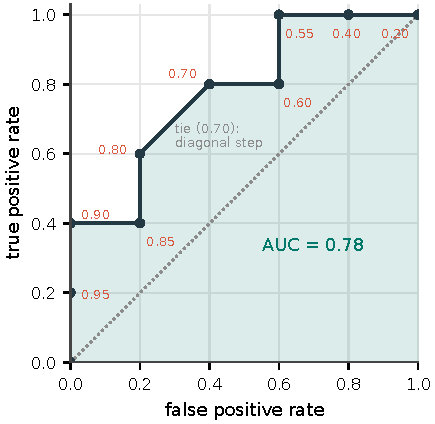
\includegraphics[width=0.56\textwidth]{ch01/roc_construction}
\caption{ROC curve of the ranking of \cref{ex:roccurve}. Each point is labelled with the
threshold that produces it; the shaded area is the AUC.}
\label{fig:roccurve}
\end{figure}

\subsection{The area under the ROC curve}

The \emph{area under the ROC curve\index{area under the ROC curve (AUC)|textbf}\index{ROC curve|textbf}} (AUC) summarises the whole curve in a single number
\citep{bradley1997use}. It has a very intuitive interpretation
\citep{hanley1982meaning}: the AUC is the probability that a randomly chosen positive
receives a higher score than a randomly chosen negative, which is the Mann--Whitney\index{Mann--Whitney--Wilcoxon statistic}--Wilcoxon
statistic \citep{mann1947test}:
\begin{equation}\label{eq:auc}
  \mathrm{AUC}=\frac{1}{P\cdot N}\sum_{i:\,y_i=+}\ \sum_{k:\,y_k=-} I\bigl(s(x_i),s(x_k)\bigr),
  \qquad
  I(a,b)=\begin{cases}1 & a>b,\\ 0.5 & a=b,\\ 0 & a<b.\end{cases}
\end{equation}
In the multiclass notation of \cref{sec:scoring}, the AUC of class $j$ against class $k$
using the probabilities estimated for class $j$ is
\begin{equation}
  \mathrm{AUC}(j,k)=\frac{\sum_{i=1}^{n}f(i,j)\sum_{t=1}^{n}f(t,k)\,I\bigl(p(i,j),p(t,j)\bigr)}{n_j\cdot n_k},
\end{equation}
where $n_j$ and $n_k$ are the numbers of examples of each class. In \cref{ex:roccurve}, 19.5 of
the 25 positive--negative pairs are correctly ordered (the tie counts one half), so
$\mathrm{AUC}=0.78$, as \cref{lst:roc} confirms.

\begin{pylisting}[label={lst:roc}]{ROC curve and AUC, computed by scikit-learn and by counting pairs}
import numpy as np
from sklearn.metrics import roc_curve, roc_auc_score

y = np.array([1, 1, 0, 1, 1, 0, 0, 1, 0, 0])                     # actual class
s = np.array([.95, .90, .85, .80, .70, .70, .60, .55, .40, .20])  # scores
fpr, tpr, thr = roc_curve(y, s)
print("FPR:", fpr.round(2))
print("TPR:", tpr.round(2))
print("AUC (scikit-learn):", roc_auc_score(y, s))

# AUC as the Mann-Whitney-Wilcoxon statistic: compare all (pos, neg) pairs
pos, neg = s[y == 1], s[y == 0]
diff = pos[:, None] - neg[None, :]
print("AUC (pairs):       ", ((diff > 0) + 0.5 * (diff == 0)).mean())
\end{pylisting}
\begin{pyoutput}
FPR: [0.  0.  0.  0.2 0.2 0.4 0.6 0.6 1. ]
TPR: [0.  0.2 0.4 0.4 0.6 0.8 0.8 1.  1. ]
AUC (scikit-learn): 0.78
AUC (pairs):        0.78
\end{pyoutput}

The AUC has several useful properties:
\begin{itemize}
  \item it is 1 for a perfect ranking, 0.5 for a random one, and below 0.5 for a ranking
        worse than random;
  \item it only depends on the order of the scores: any increasing transformation of the
        scores leaves it unchanged. It says nothing about whether the scores are good
        probabilities (\cref{sec:calibration});
  \item like the ROC curve, it does not depend on the class distribution;
  \item in credit scoring it is often reported as the \emph{Gini coefficient},
        $\mathrm{Gini}=2\,\mathrm{AUC}-1$;
  \item a crisp classifier has a ``curve'' with only three points, $(0,0)$, $(\FPR,\TPR)$
        and $(1,1)$, and its area is $(1+\TPR-\FPR)/2$, which is exactly its balanced
        accuracy\index{balanced accuracy} (Exercise~\ref{exr:aucba}).
\end{itemize}

\Cref{fig:rocmodels} compares four classifiers on the same synthetic problem. The random forest
dominates the other three almost everywhere (AUC 0.902), whereas the curves of logistic
regression (0.823) and naive Bayes\index{naive Bayes} (0.828) cross: which of the two is preferable depends on the
region of the curve where the model will operate. ROC curves are therefore very useful to
select the best model for a particular context of deployment, and the AUC is the right summary
when that context is unknown. When the relevant region is known (for instance, a screening
programme that cannot tolerate more than 10\% of false alarms) the \emph{partial} AUC over that
region is more informative.

\begin{figure}[htbp]
\centering
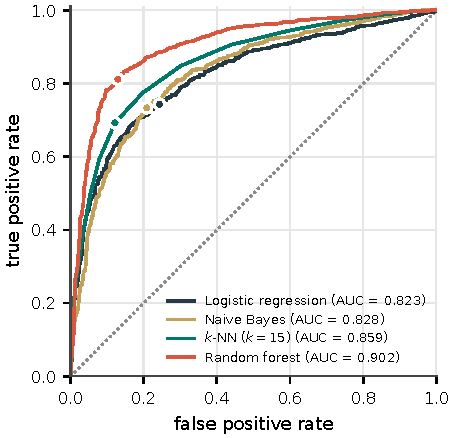
\includegraphics[width=0.6\textwidth]{ch01/roc_models}
\caption{ROC curves of four classifiers on a synthetic problem (2000 test examples). The dots
show the crisp classifiers obtained with the default threshold 0.5.}
\label{fig:rocmodels}
\end{figure}

\begin{further}
\citet{hand2009measuring} pointed out that the AUC implicitly averages over misclassification
costs using a distribution that depends on the classifier itself, and proposed the
H-measure as an alternative. \citet{hernandez2012unified} gave a unifying view: accuracy, AUC,
the Brier score\index{Brier score} and other metrics are all \emph{expected losses}, under different assumptions
about how the decision threshold will be chosen when the model is deployed. Choosing a metric
is, implicitly, choosing such an assumption.
\end{further}

\subsection{Multiclass ROC analysis}

A full ROC analysis\index{ROC analysis} with $c$ classes would need a space of $c(c-1)$ dimensions. In practice
the AUC is extended by averaging binary AUCs:
\begin{itemize}
  \item \emph{one-versus-rest}: one AUC per class against all the others, averaged either
        uniformly or weighted by the prior class distribution;
  \item \emph{one-versus-one\index{one-versus-one|textbf}}: the measure $M$ of \citet{hand2001simple} averages over all
        pairs of classes,
        \begin{equation*}
          M=\frac{2}{c(c-1)}\sum_{j<k}\hat A(j,k),\qquad
          \hat A(j,k)=\frac{\mathrm{AUC}(j,k)+\mathrm{AUC}(k,j)}{2},
        \end{equation*}
        and it is insensitive to the class distribution.
\end{itemize}
In scikit-learn, these variants are selected with the arguments \code{multi_class}
(\code{"ovr"} or \code{"ovo"}) and \code{average} (\code{"macro"} or \code{"weighted"}) of
\code{roc_auc_score}.

\subsection{Cumulative gains and lift charts}

In marketing and customer relationship management\index{customer relationship management (CRM)} (Unit~7) a model is used to rank customers,
and only the top-ranked fraction is contacted. The \emph{cumulative gains\index{cumulative gains chart|textbf} chart} plots the
fraction of all the positives (for instance, responders to a campaign\index{mailing campaign}) found among the top
$q$ fraction of the ranking, and the \emph{lift\index{lift|textbf}} is the ratio between that fraction and $q$,
i.e.\ how many times better than random targeting the model is. In the example of
\cref{fig:gains}, with 5\% of responders, contacting the top 20\% of customers reaches 76\% of
the responders, a lift of 3.78. The gains chart is closely related to the ROC curve\index{ROC curve}: its
horizontal axis is the fraction of examples predicted positive,
$\pi_+\TPR+\pi_-\FPR$, which is close to the $\FPR$ when positives are rare.

\begin{figure}[htbp]
\centering
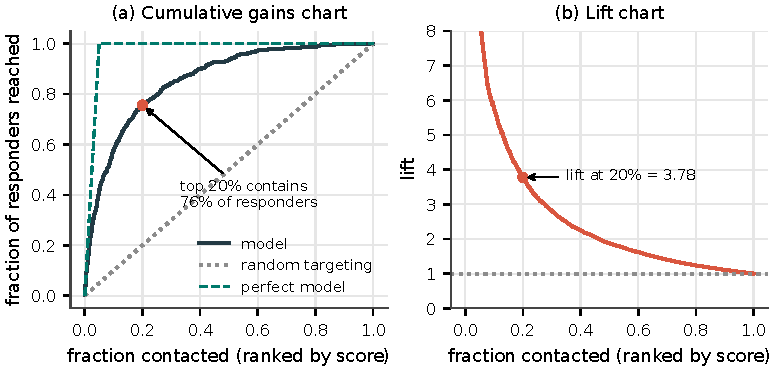
\includegraphics[width=\textwidth]{ch01/gains_lift}
\caption{Cumulative gains (a) and lift (b) of a ranking model for a mailing campaign with a 5\%
response rate (10,000 customers).}
\label{fig:gains}
\end{figure}

% ---------------------------------------------------------------------
\section{Evaluating probabilistic predictions}\label{sec:scoring}

Many applications need more than a label or a ranking: they need \emph{probabilities}. A bank
computing the expected loss of a loan, a doctor explaining a risk to a patient, or a system
combining the outputs of several models all rely on the probabilities being meaningful.

\subsection{Notation}

Consider a test set with $n$ examples and $c$ classes. Let $p(i,j)\in[0,1]$ be the probability
estimated by the model that example $i$ belongs to class $j$ (with $\sum_j p(i,j)=1$), and let
$f(i,j)\in\{0,1\}$ be the observed one-hot class indicator, which is 1 if example $i$ belongs to class $j$
and 0 otherwise. The true conditional probabilities $P(Y=j\mid x_i)$ are generally unknown: the measures
below compare the predicted probabilities with the observed outcomes. In binary problems we write $\hat p_i=p(i,+)$ and $y_i=f(i,+)$.

\subsection{Absolute error, Brier score and logarithmic loss}

The \emph{mean absolute error\index{mean absolute error (MAE)|textbf}} measures how much the predicted probabilities deviate from the
observed one-hot outcomes,
\begin{equation}
  \mathrm{MAE}=\frac{1}{n\,c}\sum_{j=1}^{c}\sum_{i=1}^{n}\bigl|f(i,j)-p(i,j)\bigr|.
\end{equation}
The \emph{mean squared error\index{mean squared error (MSE)|textbf}} is its quadratic version, which penalises strong deviations
much more:
\begin{equation}
  \mathrm{MSE}=\frac{1}{n\,c}\sum_{j=1}^{c}\sum_{i=1}^{n}\bigl(f(i,j)-p(i,j)\bigr)^2.
\end{equation}
For binary problems the two terms of the inner sum are equal and the MSE reduces to the
\emph{Brier score\index{Brier score|textbf}} \citep{brier1950verification},
$\mathrm{BS}=\frac1n\sum_i(y_i-\hat p_i)^2$.\footnote{Brier's original multiclass definition
sums over the classes without dividing by $c$, so it ranges from 0 to 2. Always check which
normalisation a library uses.}
Finally, the \emph{logarithmic loss\index{log loss|textbf}} (or cross-entropy) measures the probability assigned to
the actual class:
\begin{equation}
  \mathrm{LogLoss}=-\frac1n\sum_{i=1}^{n}\sum_{j=1}^{c}f(i,j)\log p(i,j)
                 =-\frac1n\sum_{i=1}^{n}\log p(i,y_i).
\end{equation}
It takes values in $[0,\infty)$, it is 0 only for perfect and fully confident predictions, and
it penalises confident mistakes without limit: assigning probability close to zero to the
actual class costs almost infinitely. Implementations clip the probabilities to
$[\epsilon,1-\epsilon]$ to avoid infinite values. The logarithm can be natural (as in
scikit-learn) or in base~2 (the loss is then measured in bits).

\begin{example}{Which metrics notice a better probability?}{scoringex}
A model assigns the following probabilities of being positive to five test examples:
\begin{center}\small
\begin{tabular}{@{}lccccc@{}}
\toprule
$\hat p(+)$ & 0.80 & 0.70 & 0.60 & 0.55 & 0.40\\
Actual class & $+$ & $-$ & $+$ & $+$ & $-$\\
\bottomrule
\end{tabular}
\end{center}
\begin{itemize}
  \item \emph{ROC curve\index{ROC curve|textbf} and AUC\index{area under the ROC curve (AUC)|textbf}.} With $P=3$ and $N=2$ the curve goes
        $(0,0)\to(0,\tfrac13)\to(\tfrac12,\tfrac13)\to(\tfrac12,\tfrac23)\to(\tfrac12,1)\to(1,1)$,
        and its area is $\tfrac12\cdot\tfrac13+\tfrac12\cdot1=\tfrac23$. Counting pairs gives the
        same result: of the $3\times2=6$ positive--negative pairs, four are correctly ordered.
  \item \emph{Accuracy\index{accuracy|textbf}} with threshold 0.5: only the second example is misclassified, 0.80.
  \item \emph{Brier score}:
        $(0.2^2+0.7^2+0.4^2+0.45^2+0.4^2)/5=1.0525/5=0.2105$.
\end{itemize}
If the probability of the third example increases from 0.60 to 0.68, the ranking does not
change (0.68 is still below 0.70) and neither does any prediction, so AUC and accuracy are
unchanged; but the Brier score (0.1990) and the log loss improve, because the model is now
more confident about a correct prediction (\cref{lst:scoring}).
\end{example}

\begin{pylisting}[label={lst:scoring}]{Effect of improving one probability on four metrics}
import numpy as np
from sklearn.metrics import roc_auc_score, accuracy_score, brier_score_loss, log_loss

y = np.array([1, 0, 1, 1, 0])
for p3 in (0.60, 0.68):                       # probability given to the third example
    p = np.array([0.80, 0.70, p3, 0.55, 0.40])
    print(f"p3={p3:.2f}  AUC={roc_auc_score(y, p):.3f}  "
          f"Acc={accuracy_score(y, p >= 0.5):.2f}  "
          f"Brier={brier_score_loss(y, p):.4f}  LogLoss={log_loss(y, p):.4f}")
\end{pylisting}
\begin{pyoutput}
p3=0.60  AUC=0.667  Acc=0.80  Brier=0.2105  LogLoss=0.6093
p3=0.68  AUC=0.667  Acc=0.80  Brier=0.1990  LogLoss=0.5843
\end{pyoutput}

\subsection{Proper scoring rules}

Which of these metrics actually rewards good probabilities? A \emph{scoring rule} $S(p,y)$
assigns a loss to the prediction $p$ when the outcome is $y$. It is \emph{proper} if, whenever
the true probability of the event is $q$, the expected loss $\E_{Y\sim q}[S(p,Y)]$ is minimised
by predicting $p=q$, and \emph{strictly proper} if $q$ is the only minimiser
\citep{gneiting2007strictly}. In other words, a proper scoring rule\index{proper scoring rule} never rewards a model for
reporting something different from what it believes. For a binary event:
\begin{itemize}
  \item Brier score\index{Brier score}: $\E[S]=q(1-p)^2+(1-q)p^2$, whose derivative $2(p-q)$ vanishes at $p=q$:
        strictly proper;
  \item log loss\index{log loss}: $\E[S]=-q\log p-(1-q)\log(1-p)$, whose derivative $-q/p+(1-q)/(1-p)$ vanishes
        at $p=q$: strictly proper;
  \item absolute error: $\E[S]=q(1-p)+(1-q)p=q+p(1-2q)$, which is \emph{linear} in $p$ and is
        minimised by $p=1$ if $q>1/2$ and by $p=0$ if $q<1/2$: \emph{not} proper.
\end{itemize}

\begin{keyidea}
The MAE\index{mean absolute error (MAE)} of probabilities rewards overconfidence: a model that rounds its probabilities to 0
or 1 obtains a better expected MAE than an honest one. Use the Brier score or the log loss to
judge probabilities. Both are strictly proper and, as we will see, they reward both
calibration and discrimination.
\end{keyidea}

\subsection{A taxonomy of classification metrics}

\citet{ferri2009experimental} compared 18 classification metrics experimentally over many data
sets and models, and found three families whose members are strongly correlated with each
other but much less with members of other families (\cref{tab:taxonomy}). The family to use
depends on how the model will be used.

\begin{table}[htbp]
\centering\small
\caption{Three families of classification metrics \citep{ferri2009experimental}.}\label{tab:taxonomy}
\begin{tabularx}{\textwidth}{@{}>{\raggedright\arraybackslash}p{3.2cm}>{\raggedright\arraybackslash}p{3.6cm}X@{}}
\toprule
Family & Examples & Use when\dots\\
\midrule
Threshold and qualitative understanding of error & accuracy, macro-averaged accuracy,
$F$-measure, kappa & the model makes decisions with a fixed threshold and we want to
minimise the number (or cost) of errors.\\
Probabilistic understanding of error & MAE, MSE (Brier score), log loss & we need an
assessment of the reliability of the probabilities (risk estimation, combination of models,
decisions with changing costs).\\
Ranking quality & AUC & the model prioritises cases: mailing campaigns, customer relationship
management, recommender systems, fraud detection.\\
\bottomrule
\end{tabularx}
\end{table}

\begin{example}{Metrics can disagree}{disagree}
Consider two binary classifiers $M_1$ and $M_2$ and a test set $T$. Each of the following
situations can happen, as \cref{lst:disagree} verifies:
\begin{enumerate}[label=(\alph*)]
  \item \emph{MAE\index{mean absolute error (MAE)|textbf} prefers $M_1$, MSE\index{mean squared error (MSE)|textbf} prefers $M_2$.} Two positive examples. $M_1$ predicts
        $(1.0, 0.2)$: one perfect and one bad prediction (MAE 0.40, MSE 0.32). $M_2$ predicts
        $(0.55,0.55)$: two mediocre predictions (MAE 0.45, MSE 0.20). The squared error
        punishes the single large error of $M_1$.
  \item \emph{Accuracy\index{accuracy|textbf} prefers $M_1$, MAE prefers $M_2$.} Actual classes $(+,+,-,-)$. $M_1$
        predicts $(0.51,0.51,0.49,0.49)$: all correct at threshold 0.5, but barely (accuracy
        1, MAE 0.49). $M_2$ predicts $(0.99,0.99,0.01,0.60)$: confident and almost always
        right (accuracy 0.75, MAE 0.16).
  \item \emph{Accuracy prefers $M_1$, AUC\index{area under the ROC curve (AUC)|textbf} prefers $M_2$.} Same actual classes. $M_1$ predicts
        $(0.90,0.40,0.30,0.45)$: accuracy 0.75, AUC 0.75. $M_2$ predicts $(0.90,0.80,0.70,0.60)$:
        a perfect ranking (AUC 1) with a bad threshold, since everything is predicted
        positive (accuracy 0.5).
\end{enumerate}
\end{example}

\begin{pylisting}[label={lst:disagree}]{Three pairs of models on which two metrics disagree}
import numpy as np
from sklearn.metrics import roc_auc_score

mae = lambda y, p: np.mean(np.abs(y - p))
mse = lambda y, p: np.mean((y - p) ** 2)
acc = lambda y, p: np.mean((p >= 0.5) == y)

y = np.array([1, 1])                                   # (a) MAE vs. MSE
m1, m2 = np.array([1.0, 0.2]), np.array([0.55, 0.55])
print(f"(a) MAE: {mae(y, m1):.3f} vs {mae(y, m2):.3f} | "
      f"MSE: {mse(y, m1):.3f} vs {mse(y, m2):.3f}")
y = np.array([1, 1, 0, 0])                             # (b) accuracy vs. MAE
m1, m2 = np.array([.51, .51, .49, .49]), np.array([.99, .99, .01, .60])
print(f"(b) Acc: {acc(y, m1):.2f} vs {acc(y, m2):.2f} | "
      f"MAE: {mae(y, m1):.3f} vs {mae(y, m2):.3f}")
m1, m2 = np.array([.90, .40, .30, .45]), np.array([.90, .80, .70, .60])
print(f"(c) Acc: {acc(y, m1):.2f} vs {acc(y, m2):.2f} | "    # (c) accuracy vs. AUC
      f"AUC: {roc_auc_score(y, m1):.2f} vs {roc_auc_score(y, m2):.2f}")
\end{pylisting}
\begin{pyoutput}
(a) MAE: 0.400 vs 0.450 | MSE: 0.320 vs 0.202
(b) Acc: 1.00 vs 0.75 | MAE: 0.490 vs 0.158
(c) Acc: 0.75 vs 0.50 | AUC: 0.75 vs 1.00
\end{pyoutput}

% ---------------------------------------------------------------------
\section{Calibration}\label{sec:calibration}

\subsection{What is a calibrated model?}

A binary probabilistic classifier is \emph{well calibrated\index{calibration|textbf}} if, among the examples that receive
a predicted probability $p$, the proportion of positives is approximately $p$:
\begin{equation}
  P\bigl(Y=1\mid\hat p(X)=p\bigr)=p\qquad\text{for all }p.
\end{equation}
A calibrated weather forecaster is one for whom it rains on about 70\% of the days with a 70\%
forecast. Calibration is different from discrimination (ranking quality). A model that always
predicts the prevalence\index{prevalence} is perfectly calibrated but without discrimination (it can still be a useful
reference); a model that ranks perfectly can
be badly calibrated, since any increasing transformation of its scores keeps its AUC. Good
probabilistic models need both properties, and proper scoring rules\index{proper scoring rule} reward both: the Brier
score\index{Brier score} decomposes into a calibration term and a refinement term
\citep{degroot1983comparison}.

Not all learning methods produce calibrated probabilities. Naive Bayes is a clear example: its
independence assumption counts correlated evidence several times and pushes the probabilities
towards 0 and 1. Maximum-margin methods such as SVMs output distances to a hyperplane, not
probabilities; boosted trees tend to avoid extreme values; and modern deep networks are often
overconfident \citep{niculescu2005predicting,guo2017calibration}. As we will see in
\cref{sec:imbalance}, resampling and class weights also distort the probabilities.

\subsection{Reliability diagrams}

A \emph{reliability diagram\index{calibration!reliability diagram|textbf}} (or calibration plot) groups the test examples into bins of
predicted probability and plots, for each bin, the mean predicted probability against the
observed fraction of positives. A calibrated model follows the diagonal. A histogram of the
predicted probabilities, shown alongside, tells how many examples support each point.

\Cref{fig:reliability} compares four models trained on the same data. Logistic regression,
which directly optimises the log loss\index{log loss}, is close to the diagonal. Naive Bayes concentrates its
probabilities near 0 and 1 and is \emph{overconfident}: when it predicts 0.9, the observed
frequency is much lower. The SVM, whose decision values have been naively rescaled to $[0,1]$,
is \emph{underconfident}: its outputs cluster around 0.5 while the actual frequencies are much
more extreme, which produces the typical sigmoid-shaped curve. In this example the random
forest is reasonably calibrated.

\begin{figure}[htbp]
\centering
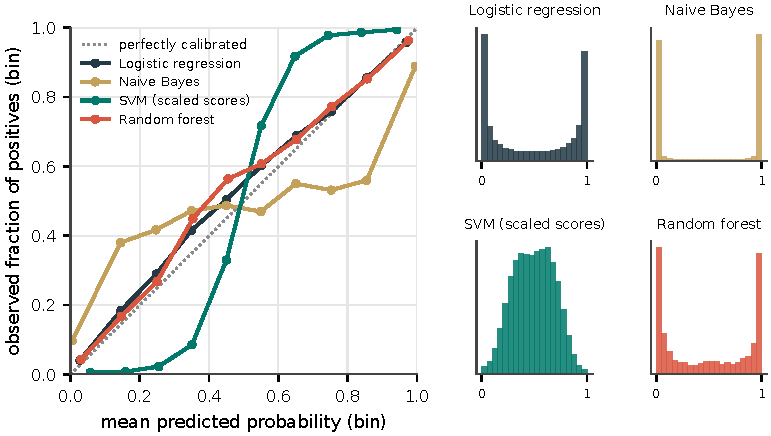
\includegraphics[width=\textwidth]{ch01/reliability}
\caption{Reliability diagrams (left) and histograms of predicted probabilities (right) of four
models trained on 1000 examples and tested on 99,000.}
\label{fig:reliability}
\end{figure}

\subsection{Measuring calibration}

Most calibration measures segment the test examples into bins and estimate the local
calibration error in each bin:
\begin{itemize}
  \item the \emph{expected calibration\index{calibration|textbf} error\index{calibration!expected calibration error|textbf}} \citep{naeini2015obtaining} averages the
        calibration gaps of $B$ bins, weighted by their sizes:
        \begin{equation}
          \mathrm{ECE}=\sum_{b=1}^{B}\frac{|S_b|}{n}\,\bigl|\bar y_b-\bar p_b\bigr|,
        \end{equation}
        where $\bar y_b$ and $\bar p_b$ are the fraction of positives and the mean predicted
        probability in bin $b$. The \emph{maximum calibration error} (MCE) takes the maximum
        gap instead. In the example of \cref{fig:reliability}, the ECE is 0.020 for logistic
        regression, 0.107 for naive Bayes\index{naive Bayes}, 0.203 for the rescaled SVM and 0.023 for the
        random forest. ECE depends on the number and type (equal width or equal frequency) of
        bins and is biased for small samples;
  \item \emph{CalBin\index{calibration!CalBin and CalLoss|textbf}} uses overlapping bins: the examples are sorted by predicted probability,
        a sliding window of consecutive examples (for instance 100) moves along the ranking,
        and the absolute differences between the mean probability and the fraction of
        positives in each window are averaged, as in the CAL measure of \citet{caruana2004data};
        other versions average the deviation of each individual prediction from the fraction of
        positives of its window \citep{ferri2009experimental}, so the variant used must be stated;
  \item \emph{CalLoss} derives the bins from the segments of the ROC convex hull\index{ROC convex hull}, which
        coincide with the blocks produced by isotonic regression\index{calibration!isotonic regression}
        \citep{fawcett2007pav}. The slope $m$ of a segment is a likelihood ratio, not a probability: with
        a proportion $\pi$ of positives, the empirical probability of the positive class in the
        segment is $m\pi/(m\pi+1-\pi)$ (for instance $2/3$ for $m=2$ and balanced classes). The
        calibration loss is the mean squared deviation between the predicted probabilities and
        these empirical probabilities; \citet{ferri2009experimental} group equal predicted
        probabilities instead of hull segments, so here too the variant must be stated. A measure
        computed on evaluation data is a diagnostic; a calibrator to deploy must be fitted on
        separate calibration data;
  \item the MSE\index{mean squared error (MSE)} and the log loss\index{log loss} also measure calibration, mixed with discrimination. For
        forecasts that take $K$ distinct values $p_k$ ($n_k$ examples each, with a fraction
        $\bar y_k$ of positives, and an overall fraction $\bar y$), the Brier score\index{Brier score} decomposes
        exactly \citep{murphy1973new} as
        \begin{equation}\label{eq:murphy}
          \mathrm{BS}=\underbrace{\frac1n\sum_k n_k(p_k-\bar y_k)^2}_{\text{reliability}}
                     -\underbrace{\frac1n\sum_k n_k(\bar y_k-\bar y)^2}_{\text{resolution}}
                     +\underbrace{\bar y(1-\bar y)}_{\text{uncertainty}}.
        \end{equation}
        Reliability measures calibration (lower is better), resolution measures how well the
        forecasts separate cases with different outcome frequencies (higher is better), and
        uncertainty depends only on the data. Grouping the uncertainty and the resolution
        gives the decomposition of the Brier score into \emph{calibration} and
        \emph{refinement} \citep{degroot1983comparison}. With continuous forecasts, binning
        makes the decomposition approximate.
\end{itemize}

\begin{pitfall}
\textbf{Small samples flatter hulls and calibration errors.} On small or very imbalanced\index{class imbalance} validation sets, the
convex hull of noisy ROC points, the isotonic fit behind CalLoss and the bins of the ECE all adapt to the noise:
the area under the hull is optimistic, and the calibration errors are biased (the ECE is positive even for a
perfectly calibrated model). Estimate them on data that took no part in fitting the hull or the calibrator, and
report their variability, for instance with the bootstrap\index{bootstrap}.
\end{pitfall}

\subsection{Calibration methods}

\emph{Calibrating} a classifier consists of fitting a regressor (the \emph{calibrator}) that
maps the scores of the classifier to calibrated probabilities. The examples used to train the
calibrator must not have been used to train the classifier, because scores on training data
are optimistic; scikit-learn's \code{CalibratedClassifierCV} handles this with an internal
cross-validation. The most common calibrators are:
\begin{itemize}
  \item \emph{Platt scaling\index{calibration!Platt scaling|textbf}} \citep{platt1999probabilistic}: a logistic regression on the
        score $s$, $\hat p=1/\bigl(1+\exp(As+B)\bigr)$, with $A$ and $B$ fitted by maximum
        likelihood. It has only two parameters, needs little data and corrects
        sigmoid-shaped distortions such as those of SVMs;
  \item \emph{isotonic regression\index{calibration!isotonic regression|textbf}} \citep{zadrozny2002transforming}: fits a non-parametric,
        non-decreasing step function with the pool-adjacent-violators (PAV) algorithm. It can
        correct any monotone distortion but needs more data, since it can overfit small
        calibration sets. It is equivalent to calibrating with the ROC convex hull\index{ROC convex hull}
        \citep{fawcett2007pav};
  \item \emph{temperature scaling} \citep{guo2017calibration}: for multiclass neural networks,
        divides the logits $z$ by a single parameter $T>0$ fitted on validation data,
        $\hat p=\operatorname{softmax}(z/T)$. It does not change the predicted class, so the
        accuracy is unchanged. It mainly improves \emph{confidence} (top-label) calibration,
        $P(Y=\hat y\mid\max_j\hat p_j=p)=p$; \emph{classwise} calibration, $P(Y=j\mid\hat p_j=p)=p$ for every
        class $j$, is a stronger requirement that a single parameter cannot always meet, which motivates
        vector, matrix and Dirichlet calibration \citep{kull2019beyond};
  \item \emph{beta calibration\index{calibration|textbf}} \citep{kull2017beta}: a three-parameter family that contains
        the identity map, designed for scores that are already in $[0,1]$.
\end{itemize}

\Cref{fig:calibmethods} calibrates an SVM like that of \cref{fig:reliability}, trained on a different sample: Platt scaling reduces
the ECE\index{calibration!expected calibration error} from 0.285 to 0.032 and isotonic regression to 0.007. \Cref{lst:calibration} does the
same for naive Bayes\index{naive Bayes} and reports the three probabilistic metrics: the log loss\index{log loss} falls from 1.15
to 0.28, mostly because the overconfident mistakes disappear. A strictly increasing
calibrator applied to a fixed score preserves the ranking and the AUC. Isotonic regression can
introduce ties, and when, as in the listing, the calibrated probabilities of models fitted on
different folds are averaged, the ranking can also change; here the AUC hardly moves. Calibration matters most when the probabilities are used
to take decisions, as in \cref{sec:costs}.

\begin{figure}[htbp]
\centering
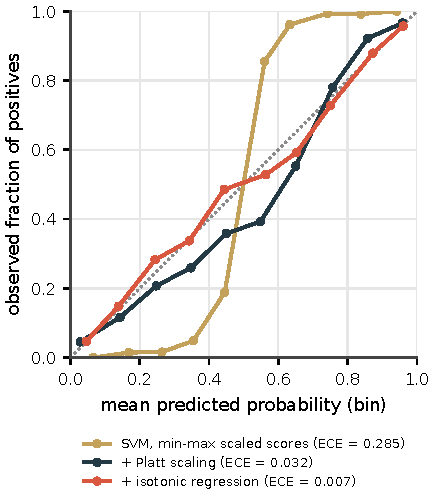
\includegraphics[width=0.56\textwidth]{ch01/calibration_methods}
\caption{Reliability diagrams of a linear SVM with naively rescaled scores, and of the same
model calibrated with Platt scaling and isotonic regression (20,000 test examples).}
\label{fig:calibmethods}
\end{figure}

\begin{pylisting}[label={lst:calibration}]{Calibrating naive Bayes with Platt scaling and isotonic regression}
import numpy as np
from sklearn.calibration import CalibratedClassifierCV
from sklearn.datasets import make_classification
from sklearn.metrics import brier_score_loss, log_loss
from sklearn.model_selection import train_test_split
from sklearn.naive_bayes import GaussianNB

def ece(y, p, n_bins=10):
    """Expected calibration error with equal-width bins."""
    b = np.minimum((p * n_bins).astype(int), n_bins - 1)
    return sum(np.mean(b == k) * abs(y[b == k].mean() - p[b == k].mean())
               for k in range(n_bins) if np.any(b == k))

X, y = make_classification(n_samples=40000, n_features=20, n_informative=2,
                           n_redundant=10, random_state=42)
X_tr, X_te, y_tr, y_te = train_test_split(X, y, test_size=0.5, random_state=0)
models = {"NB": GaussianNB(),
          "NB + Platt": CalibratedClassifierCV(GaussianNB(), method="sigmoid", cv=5),
          "NB + isotonic": CalibratedClassifierCV(GaussianNB(), method="isotonic", cv=5)}
for name, m in models.items():
    p = m.fit(X_tr, y_tr).predict_proba(X_te)[:, 1]
    print(f"{name:14s} Brier={brier_score_loss(y_te, p):.4f}  "
          f"LogLoss={log_loss(y_te, p):.4f}  ECE={ece(y_te, p):.4f}")
\end{pylisting}
\begin{pyoutput}
NB             Brier=0.1050  LogLoss=1.1476  ECE=0.1009
NB + Platt     Brier=0.0960  LogLoss=0.3342  ECE=0.0171
NB + isotonic  Brier=0.0849  LogLoss=0.2809  ECE=0.0068
\end{pyoutput}

% ---------------------------------------------------------------------
\section{Imbalanced classification}\label{sec:imbalance}

In many important problems one class is rare: fraud, diseases, machine failures, customers
who respond to a campaign\index{mailing campaign}. Imbalance\index{class imbalance} affects both evaluation and learning.

\subsection{Why accuracy fails}

\begin{example}{Detecting a rare event}{valves}
A plant monitors 100,000 safety valves, of which 500 (0.5\%) are faulty (\emph{open}) and must
be inspected; the rest are \emph{closed}. Three classifiers produce these confusion matrices\index{confusion matrix}
(rows: predicted; columns: actual):
\begin{center}\small
\begin{tabular}{@{}lcc@{\qquad}lcc@{\qquad}lcc@{}}
\toprule
$c_1$ & open & close & $c_2$ & open & close & $c_3$ & open & close\\
\midrule
OPEN  & 300 & 500    & OPEN  & 0   & 0      & OPEN  & 400 & 5400\\
CLOSE & 200 & 99,000 & CLOSE & 500 & 99,500 & CLOSE & 100 & 94,100\\
\bottomrule
\end{tabular}
\end{center}
Their metrics are:
\begin{center}\small
\begin{tabular}{@{}lccc@{}}
\toprule
& $c_1$ & $c_2$ & $c_3$\\
\midrule
Error & 0.70\% & \textbf{0.50\%} & 5.50\%\\
TPR\index{true positive rate} / TNR & 60.0\% / 99.5\% & 0.0\% / 100\% & 80.0\% / 94.6\%\\
PPV\index{predictive value!positive} / NPV\index{predictive value!negative} & 37.5\% / 99.8\% & undefined / 99.5\% & 6.9\% / 99.9\%\\
Balanced accuracy\index{balanced accuracy} & 79.8\% & 50.0\% & \textbf{87.3\%}\\
G-mean & 0.773 & 0 & \textbf{0.870}\\
$F_1$ & \textbf{0.462} & 0 & 0.127\\
MCC\index{Matthews correlation coefficient} & \textbf{0.471} & 0 & 0.225\\
Kappa & \textbf{0.458} & 0 & 0.119\\
\bottomrule
\end{tabular}
\end{center}
The classifier with the lowest error, $c_2$, never detects a faulty valve: it simply predicts
the majority class. Balanced accuracy and the G-mean prefer $c_3$, which finds 80\% of the
faulty valves at the price of 5400 unnecessary inspections. $F_1$, MCC and kappa prefer $c_1$,
which is much more precise. Which one is better? The metrics cannot tell; only the
consequences of each type of error can. We will come back to this example in
\cref{sec:costs}.
\end{example}

\begin{keyidea}
When classes are imbalanced\index{class imbalance}, avoid metrics centred only on counting mistakes (accuracy,
error): the trivial majority classifier is hard to beat on them. Recommended alternatives are
the AUC and the average precision\index{average precision} for rankings, and the $F_1$ score, balanced accuracy,
G-mean and MCC for crisp decisions, ideally complemented by an explicit cost analysis.
\end{keyidea}

\subsection{Precision--recall analysis}

The \emph{precision\index{precision|textbf}--recall\index{recall|textbf}} (PR) curve plots precision against recall for all thresholds, and
the \emph{average precision\index{average precision|textbf}} (AP) summarises it as a step-wise area,
$\mathrm{AP}=\sum_k(R_k-R_{k-1})P_k$, where $P_k$ and $R_k$ are the precision and recall at the
$k$-th threshold. Unlike the ROC curve\index{ROC curve}, the PR curve depends on the class distribution: the
precision of a random classifier equals the prevalence\index{prevalence}. This is exactly why it is informative
with rare positives \citep{saito2015precision}. In \cref{fig:prvsroc} the same score
distributions are evaluated with 50\% and 2\% of positives. The ROC curves are almost
identical (AUC 0.857 and 0.862), but the average precision drops from 0.855 to 0.213: with
many negatives, even a small false positive rate\index{false positive rate} produces many false alarms, and most positive
predictions are wrong. The ROC curve hides this; the PR curve shows it.

\begin{figure}[htbp]
\centering
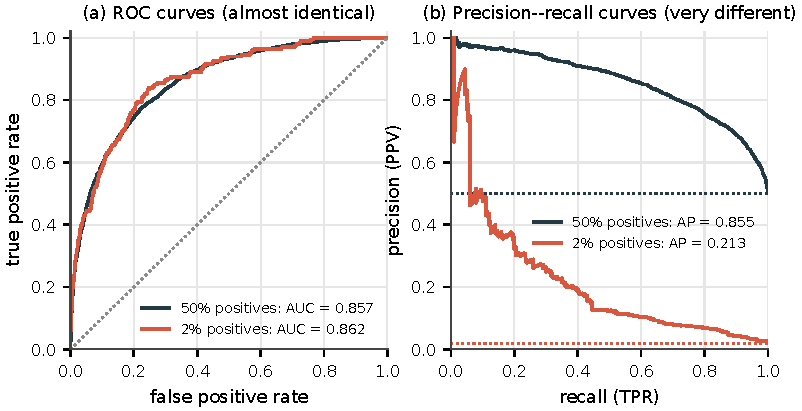
\includegraphics[width=\textwidth]{ch01/pr_vs_roc}
\caption{The same scoring model evaluated with 50\% and with 2\% of positives. (a) ROC curves
do not depend on the class distribution. (b) Precision--recall curves do; the dotted lines are
the precision of a random classifier (the prevalence).}
\label{fig:prvsroc}
\end{figure}

\citet{davis2006relationship} proved that a curve dominates another in ROC space\index{ROC space} if and only
if it dominates it in PR space, but that linear interpolation between points, valid in ROC
space, is not valid in PR space. This is why AP is computed as a step-wise sum rather than
with the trapezoidal rule.

\subsection{Learning from imbalanced data}

Many learning methods minimise the number of mistakes, and the learned models may simply
ignore the minority class \citep{japkowicz2002class,he2009learning}. The main remedies are:
\begin{itemize}
  \item \emph{undersampling\index{undersampling|textbf}} the majority class, which is fast but removes useful
        information;
  \item \emph{oversampling\index{oversampling|textbf}} the minority class by replication, which creates redundant
        examples and encourages overfitting;
  \item \emph{learning with costs or weights}, which minimises the (weighted) cost instead of
        the number of errors; in scikit-learn, \code{class_weight="balanced"} weights each
        class inversely to its frequency;
  \item \emph{synthetic oversampling}, which creates new minority examples.
\end{itemize}

The best known synthetic method is SMOTE\index{SMOTE}, the Synthetic Minority Oversampling Technique
\citep{chawla2002smote}. To create each synthetic example, SMOTE chooses a random minority
example, finds its $k$ (usually 5) nearest neighbours\index{k-nearest neighbours@$k$-nearest neighbours} of the same class, picks one of them at
random and creates a new example at a random point of the segment that joins the two
(\cref{fig:smote}). The core of the algorithm takes a few lines (\cref{lst:smote}).
Variants concentrate the new examples where they are most useful: Borderline-SMOTE near the
class boundary \citep{han2005borderline} and ADASYN where the minority class is harder to learn
\citep{he2008adasyn}. ROSE \citep{menardi2014training} uses a \emph{smoothed bootstrap\index{bootstrap|textbf}}
instead: it draws an example (choosing each class with equal probability) and generates a new
one from a kernel density centred on it, that is, from its neighbourhood.

\begin{figure}[htbp]
\centering
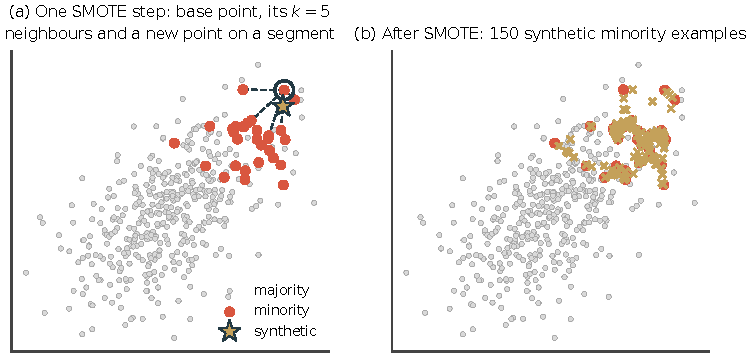
\includegraphics[width=\textwidth]{ch01/smote}
\caption{SMOTE. (a) A minority example (circled), its five nearest minority neighbours and a
synthetic example generated on one of the segments. (b) The data after adding 150 synthetic
examples.}
\label{fig:smote}
\end{figure}

\begin{pylisting}[label={lst:smote}]{A minimal implementation of SMOTE}
import numpy as np
from sklearn.neighbors import NearestNeighbors

def smote(X_min, n_new, k=5, seed=0):
    """Generate n_new synthetic minority examples (Chawla et al., 2002)."""
    rng = np.random.default_rng(seed)
    nn = NearestNeighbors(n_neighbors=k + 1).fit(X_min)
    _, idx = nn.kneighbors(X_min)                 # idx[:, 0] is the point itself
    base = rng.integers(0, len(X_min), n_new)      # random minority examples
    neigh = idx[base, rng.integers(1, k + 1, n_new)]   # one of their k neighbours
    gap = rng.random((n_new, 1))                   # random position on the segment
    return X_min[base] + gap * (X_min[neigh] - X_min[base])
\end{pylisting}

\begin{pitfall}
Resample only the training data. If SMOTE or any other resampling is applied before splitting
the data or before cross-validation, synthetic copies of test examples end up in the training
set and the evaluation is optimistic. The \code{Pipeline} of \textsf{imbalanced\index{class imbalance}-learn}
\citep{lemaitre2017imbalanced} applies the resampling only when fitting, inside each fold.
\end{pitfall}

\subsection{What rebalancing really does}

\Cref{lst:imbalance} compares, with 5-fold CV on a problem with about 3.5\% of positives (3\% before the label noise\index{label noise}
of the generator), a plain
logistic regression, a class-weighted one and SMOTE\index{SMOTE} followed by logistic regression. Rebalancing
increases the balanced accuracy\index{balanced accuracy} (from 0.60 to about 0.70) but \emph{decreases} the $F_1$ score
(from 0.33 to 0.15), slightly decreases the average precision\index{average precision}, and multiplies the Brier score\index{Brier score}
by seven.

\begin{pylisting}[label={lst:imbalance}]{Effect of class weights and SMOTE on four metrics}
from imblearn.over_sampling import SMOTE
from imblearn.pipeline import make_pipeline     # resamples ONLY the training folds
from sklearn.datasets import make_classification
from sklearn.linear_model import LogisticRegression
from sklearn.model_selection import StratifiedKFold, cross_validate

X, y = make_classification(n_samples=10000, n_features=10, n_informative=4,
                           weights=[0.97], flip_y=0.01, class_sep=1.5, random_state=0)
cv = StratifiedKFold(5, shuffle=True, random_state=0)
lr = lambda **kw: LogisticRegression(max_iter=1000, **kw)
models = {"plain LR": lr(),
          "weighted LR": lr(class_weight="balanced"),
          "SMOTE + LR": make_pipeline(SMOTE(random_state=0), lr())}
scoring = ["balanced_accuracy", "f1", "average_precision", "neg_brier_score"]
for name, m in models.items():
    r = cross_validate(m, X, y, cv=cv, scoring=scoring)
    print(f"{name:11s} BA={r['test_balanced_accuracy'].mean():.3f} "
          f"F1={r['test_f1'].mean():.3f} AP={r['test_average_precision'].mean():.3f} "
          f"Brier={-r['test_neg_brier_score'].mean():.4f}")
\end{pylisting}
\begin{pyoutput}
plain LR    BA=0.601 F1=0.331 AP=0.432 Brier=0.0250
weighted LR BA=0.697 F1=0.150 AP=0.377 Brier=0.1800
SMOTE + LR  BA=0.694 F1=0.148 AP=0.373 Brier=0.1771
\end{pyoutput}

In this experiment, rebalancing acts mostly like \emph{moving the decision threshold\index{threshold|textbf}}: the
rebalanced model predicts many more positives (more true positives and many more false
positives) without ranking the examples better. This is common but not guaranteed: changing the
weights or the sample also changes the fitted model, and with it the ranking, in ways that depend
on the learner and on the sampling method. And because the model has learned that positives are as
frequent as negatives, its probabilities no longer describe the original population. Under pure
prior shift\index{label shift}, when the class-conditional distributions do not change, the probabilities of a model
trained with a prevalence\index{prevalence} $\pi'$ can be corrected for a population with prevalence $\pi$ (random
sampling of whole classes approximates this situation; after SMOTE or other feature-dependent
sampling, recalibrate on data representative of deployment instead)
\citep{saerens2002adjusting,elkan2001foundations}:
\begin{equation}\label{eq:priorshift}
  \hat p=\frac{\frac{\pi}{\pi'}\,\hat p'}{\frac{\pi}{\pi'}\,\hat p'+\frac{1-\pi}{1-\pi'}\,(1-\hat p')}.
\end{equation}
For example, a model trained on balanced data ($\pi'=0.5$) that outputs $\hat p'=0.5$ for a
case from a population with $\pi=0.03$ corresponds to $\hat p=0.03$. In clinical risk
prediction, \citet{vandengoorbergh2022harm} showed that imbalance\index{class imbalance} corrections worsened the
calibration of logistic regression models without improving their discrimination.

\begin{keyidea}
Class imbalance is as much a problem of evaluation and decision as of learning. Often the
best strategy is to keep the data as they are, obtain calibrated probabilities, evaluate with
metrics suited to rare classes, and choose the threshold according to the costs
(\cref{sec:costs}).
\end{keyidea}

% ---------------------------------------------------------------------
\section{Cost-sensitive evaluation and learning}\label{sec:costs}

\subsection{Cost matrices}

Not all mistakes have the same consequences. In COVID-19 detection a false negative (an
infected person sent home) is much worse than a false positive (an unnecessary quarantine). In
credit granting, if the positive class is ``grant the loan'', a false positive (lending to
someone who will not pay back) usually costs much more than a false negative (losing the
margin of a good customer). A \emph{cost matrix\index{cost matrix|textbf}} $C$ states the cost of every possible
decision: $C(i,j)$ is the cost of predicting class $i$ when the actual class is $j$. It has the
same layout as the confusion matrix\index{confusion matrix} $M$, and the total cost of a classifier on a test set is
\begin{equation}
  \text{Cost}=\sum_{i=1}^{c}\sum_{j=1}^{c}C(i,j)\,M(i,j).
\end{equation}
Negative entries represent benefits.

\begin{example}{Total cost of a three-class model}{cost3}
A model classifies cases into three levels (\emph{low}, \emph{medium}, \emph{high}). The cost
matrix (left) and the confusion matrix on a test set (right), both with predicted classes in
rows and actual classes in columns, are:
\begin{center}\small
\begin{tabular}{@{}lrrr@{}}
\toprule
Cost & low & medium & high\\
\midrule
low    & 0\EUR    & 5\EUR      & 2\EUR\\
medium & 200\EUR  & $-2000$\EUR & 10\EUR\\
high   & 10\EUR   & 1\EUR      & $-15$\EUR\\
\bottomrule
\end{tabular}\qquad
\begin{tabular}{@{}lrrr@{}}
\toprule
Count & low & medium & high\\
\midrule
low    & 20 & 0  & 13\\
medium & 5  & 15 & 4\\
high   & 4  & 7  & 60\\
\bottomrule
\end{tabular}
\end{center}
Row by row, the costs are $0\cdot20+5\cdot0+2\cdot13=26$\EUR,
$200\cdot5-2000\cdot15+10\cdot4=-28{,}960$\EUR{} and $10\cdot4+1\cdot7-15\cdot60=-853$\EUR, so
the total cost is $-29{,}787$\EUR: the model produces a net benefit, almost entirely due to the
15 correctly identified \emph{medium} cases.
\end{example}

Returning to the valves of \cref{ex:valves}, suppose that an unnecessary inspection costs
100\EUR{} and an undetected faulty valve costs 2000\EUR. The total costs are
$500\cdot100+200\cdot2000=450{,}000$\EUR{} for $c_1$, $500\cdot2000=1{,}000{,}000$\EUR{} for
$c_2$ and $5400\cdot100+100\cdot2000=740{,}000$\EUR{} for $c_3$. Classifier $c_1$ is the best
choice, and $c_3$, preferred by balanced accuracy\index{balanced accuracy}, costs 64\% more.

\subsection{Optimal decisions from probabilities}

If a model provides calibrated probabilities $p(j\mid x)$, the expected cost\index{expected cost} of predicting
class $i$ for example $x$ is $\sum_j p(j\mid x)\,C(i,j)$, and the optimal decision is the class
with the lowest expected cost. With two classes and costs $c_{ij}$ (predicted $i$, actual $j$,
with 1 the positive class), predicting positive is optimal when
$p\,c_{11}+(1-p)\,c_{10}\leq p\,c_{01}+(1-p)\,c_{00}$, that is, when the probability of the
positive class exceeds the threshold
\begin{equation}\label{eq:tstar}
  t^\star=\frac{c_{10}-c_{00}}{(c_{10}-c_{00})+(c_{01}-c_{11})}
  \quad\text{or, if correct decisions cost nothing,}\quad
  t^\star=\frac{c_{\mathrm{FP}}}{c_{\mathrm{FP}}+c_{\mathrm{FN}}}
\end{equation}
\citep{elkan2001foundations}. For the valves, $t^\star=100/2100=0.048$: a valve should be
inspected whenever its probability of being open exceeds 4.8\%, far from the default 0.5.
\Cref{lst:costthreshold} applies this rule to a logistic regression on a problem with 3\% of
positives: moving the threshold from 0.5 to $t^\star$ multiplies the false positives by 200
but reduces the total cost by 32\%. \Cref{fig:costthreshold} shows the empirical cost as a
function of the threshold for three cost ratios; the minima are close to the theoretical
thresholds because logistic regression is well calibrated.

\begin{pylisting}[label={lst:costthreshold}]{Cost of the default threshold versus the Bayes-optimal one}
import numpy as np
from sklearn.datasets import make_classification
from sklearn.linear_model import LogisticRegression
from sklearn.model_selection import train_test_split

C_FP, C_FN = 100, 2000           # cost of a false alarm and of a missed positive
t_star = C_FP / (C_FP + C_FN)    # Bayes-optimal threshold for calibrated scores

X, y = make_classification(n_samples=40000, n_features=10, n_informative=5,
                           weights=[0.97], flip_y=0.01, random_state=3)
X_tr, X_te, y_tr, y_te = train_test_split(X, y, test_size=0.5, stratify=y,
                                          random_state=0)
p = LogisticRegression(max_iter=1000).fit(X_tr, y_tr).predict_proba(X_te)[:, 1]

def total_cost(y, yhat):
    return C_FP * np.sum((yhat == 1) & (y == 0)) + C_FN * np.sum((yhat == 0) & (y == 1))

for t in (0.5, t_star):
    yhat = (p >= t).astype(int)
    print(f"t={t:.4f}  FP={np.sum((yhat == 1) & (y_te == 0)):4d}  "
          f"FN={np.sum((yhat == 0) & (y_te == 1)):3d}  "
          f"cost={total_cost(y_te, yhat):>9,} EUR")
\end{pylisting}
\begin{pyoutput}
t=0.5000  FP=  14  FN=572  cost=1,145,400 EUR
t=0.0476  FP=3070  FN=235  cost=  777,000 EUR
\end{pyoutput}

\begin{figure}[htbp]
\centering
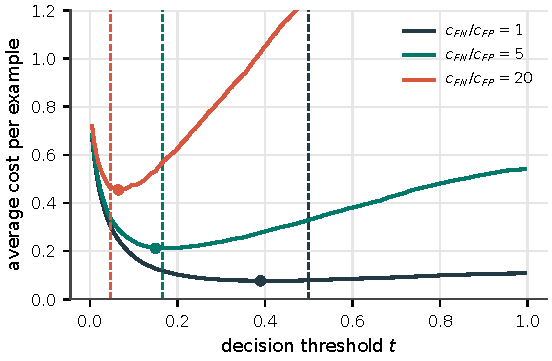
\includegraphics[width=0.7\textwidth]{ch01/cost_threshold}
\caption{Average cost per example (in units of $c_{\mathrm{FP}}$) as a function of the decision
threshold, for three cost ratios. Dashed lines: theoretical optimum $t^\star=1/(1+c_{\mathrm{FN}}/c_{\mathrm{FP}})$;
dots: empirical minimum.}
\label{fig:costthreshold}
\end{figure}

The same reasoning applies to more classes. With the cost matrix\index{cost matrix} of \cref{ex:cost3} and a case
with probabilities $(0.5, 0.3, 0.2)$ for \emph{low}, \emph{medium} and \emph{high}, the expected
costs are $0\cdot0.5+5\cdot0.3+2\cdot0.2=1.9$\EUR{} for predicting \emph{low},
$200\cdot0.5-2000\cdot0.3+10\cdot0.2=-498$\EUR{} for \emph{medium} and
$10\cdot0.5+1\cdot0.3-15\cdot0.2=2.3$\EUR{} for \emph{high}: the best decision is
\emph{medium}, although \emph{low} is the most probable class.

\subsection{Cost curves}

ROC space\index{ROC space} shows costs only indirectly, through the slopes of the iso-performance lines.
\emph{Cost curves\index{cost curve|textbf}} \citep{drummond2006cost} show them directly. The horizontal axis is the
\emph{probability cost}
\begin{equation}
  PC(+)=\frac{\pi_+\,c_{\mathrm{FN}}}{\pi_+\,c_{\mathrm{FN}}+\pi_-\,c_{\mathrm{FP}}}\in[0,1],
\end{equation}
which summarises the operating condition\index{operating point} (class distribution and costs) in a single number,
and the vertical axis is the \emph{normalised expected cost\index{expected cost|textbf}}
$\mathrm{NEC}=\FNR\cdot PC(+)+\FPR\cdot\bigl(1-PC(+)\bigr)$. Each classifier becomes a straight
line from $(0,\FPR)$ to $(1,\FNR)$; AlwaysNeg is the line $\mathrm{NEC}=PC(+)$ and AlwaysPos
the line $\mathrm{NEC}=1-PC(+)$. The lower envelope of all the lines gives the best achievable
cost for every operating condition, and it is the exact counterpart (the dual) of the ROC
convex hull\index{ROC convex hull}: points of ROC space become lines, and vertices of the hull become segments of the
envelope. \Cref{fig:costcurves} shows the five classifiers of \cref{ex:rochull}: we can read
directly the range of conditions in which each classifier is optimal and by how much it
improves on the others.

\begin{figure}[htbp]
\centering
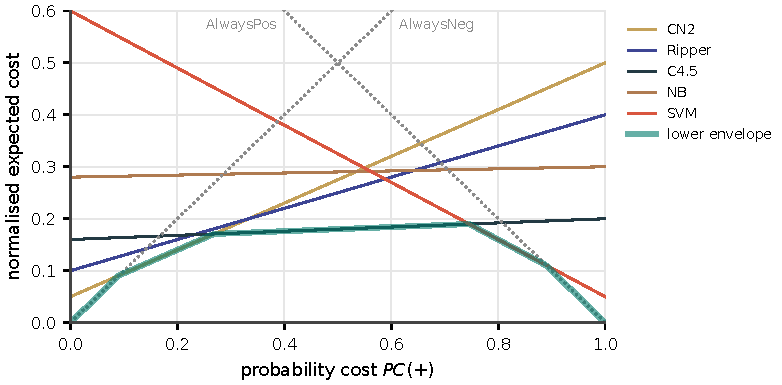
\includegraphics[width=0.75\textwidth]{ch01/cost_curves}
\caption{Cost curves of the five classifiers of \cref{ex:rochull}. The thick line is the lower
envelope, which corresponds to the ROC convex hull of \cref{fig:rochull}.}
\label{fig:costcurves}
\end{figure}

\subsection{Cost-sensitive learning strategies}

There are four main ways of making a learning process sensitive to costs:
\begin{enumerate}
  \item \emph{Expected cost\index{expected cost|textbf} minimisation (thresholding).} Train an ordinary probabilistic
        model, calibrate it if needed, and predict the class of minimum expected cost
        (\cref{eq:tstar}). It is simple, it works with any probabilistic model, and the
        costs can be changed after training.
  \item \emph{Resampling.} Change the class proportions of the training set so that a learner
        using the default threshold behaves as if it used $t^\star$. \citet{elkan2001foundations}
        showed that, if correct decisions cost nothing, the number of negative examples must be
        multiplied by $c_{\mathrm{FP}}/c_{\mathrm{FN}}$ (or, equivalently, positives replicated
        $c_{\mathrm{FN}}/c_{\mathrm{FP}}$ times). For the valves, one negative in every 20.
  \item \emph{Weighting.} Give each training example a weight proportional to the cost of
        misclassifying it \citep{zadrozny2003cost}. Most scikit-learn estimators accept
        \code{class_weight} or \code{sample_weight} for this purpose.
  \item \emph{Cost-sensitive\index{cost-sensitive learning|textbf} algorithms.} MetaCost\index{MetaCost} \citep{domingos1999metacost} estimates the
        class probabilities of the training examples with a bagged ensemble, relabels each
        training example with the class of minimum expected cost and retrains the base
        learner on the relabelled data, producing a single cost-sensitive model of the
        original type. AdaCost \citep{fan1999adacost} modifies boosting so that the weights of
        costly misclassified examples increase faster.
\end{enumerate}

\subsection{Other types of cost}

Misclassification costs are not the only costs. \citet{turney2000types} proposed a taxonomy of
nine types of cost in inductive learning, among which:
\begin{itemize}
  \item the cost of \emph{misclassification errors} (or prediction errors in general);
  \item the cost of \emph{tests}: obtaining the value of an attribute may require a laboratory
        analysis, a sensor or a questionnaire;
  \item the cost of the \emph{teacher}: labelling examples requires experts, which motivates
        active and semi-supervised\index{semi-supervised learning} learning;
  \item the cost of \emph{computation}: training and prediction time, memory and energy, which
        matter at deployment time (Unit~5);
  \item the cost of \emph{cases}: collecting data;
  \item the cost of \emph{instability}: models that change substantially when the data change
        slightly are hard to trust and to maintain, which is closely related to concept drift\index{concept drift}
        and to the need to update models (Unit~6).
\end{itemize}

\subsection{Test costs}

Knowing the exact value of some features has a cost. To diagnose a heart condition, the age of
the patient is free, the blood pressure is cheap and the cholesterol level requires a blood test.
When tests are costly, we want models that minimise the expected test cost\index{test costs} while keeping their
predictive performance. A model that needs every feature for every case, as most ensembles and
neural networks do, pays the full cost every time. A decision tree\index{decision tree} only asks for the tests on
the path followed by each case, and it can be induced to prefer cheap tests near the root
\citep{nunez1991use,turney1995cost}. For example, if a tree asks for the free attribute first,
for the blood pressure (5\EUR) in 60\% of the cases and for the cholesterol (40\EUR) in 20\%,
its expected test cost is $0.6\cdot5+0.2\cdot40=11$\EUR{} per patient, against 45\EUR{} for a
model that always requires all the tests. Evaluation should then report the expected
misclassification cost and the expected test cost together.

\subsection{Instance-dependent costs}

In some domains the cost of an error is not constant but varies from example to example.
\citet{elkan2001foundations} gives the example of credit card transactions, where $x$ is the
amount of the transaction. Here it is more convenient to use a \emph{benefit} matrix $B$ rather than a cost
matrix\index{cost matrix}: positive entries are gains and negative entries losses, and the optimal decision maximises the
expected benefit (equivalently, it minimises the costs $C=-B$):
\begin{center}\small
\begin{tabular}{@{}lcc@{}}
\toprule
{\footnotesize decision\,\textbackslash\,actual} & fraudulent & legitimate\\
\midrule
refuse  & $20$\EUR & $-20$\EUR\\
approve & $-x$     & $0.02\,x$\\
\bottomrule
\end{tabular}
\end{center}
Refusing a fraudulent transaction saves investigation and charge-back costs; refusing a
legitimate one annoys the customer; approving a fraudulent one loses the amount; approving a
legitimate one earns a 2\% commission. If $p$ is the probability of fraud, approving is better
than refusing when $0.02x(1-p)-xp>20p-20(1-p)$, that is, when
\begin{equation}
  p<\frac{0.02\,x+20}{1.02\,x+40}.
\end{equation}
The threshold is 0.40 for a 10\EUR{} transaction, 0.15 for 100\EUR{} and only 0.038 for
1000\EUR: large transactions are refused at much lower probabilities of fraud. During learning,
a simple approach is to re-weight each training example in proportion to its own
misclassification cost \citep{zadrozny2003cost}.

% ---------------------------------------------------------------------
\section{Evaluating regression models}\label{sec:regression}

In regression the model predicts a number, and the errors $e_i=\hat y_i-y_i$ have a magnitude
and a sign. Regression metrics differ in how they aggregate them.

\subsection{A worked example}

\Cref{tab:regex} shows the predictions of a model of the annual sales of ten companies (in
millions of euros). We will use it to illustrate all the metrics of this section.

\begin{table}[htbp]
\centering\small
\caption{Predicted and actual annual sales of ten companies (million \texteuro), with the
error $e=\hat y-y$ and its square.}\label{tab:regex}
\begin{tabular}{@{}lrrrrrrrrrr|r@{}}
\toprule
Company & 1 & 2 & 3 & 4 & 5 & 6 & 7 & 8 & 9 & 10 & Sum\\
\midrule
Predicted $\hat y$ & 100 & 102 & 105 & 95 & 101 & 105 & 105 & 40 & 220 & 100 &\\
Actual $y$         & 102 & 110 & 95  & 75 & 103 & 110 & 98  & 32 & 215 & 103 &\\
Error $e$          & $-2$ & $-8$ & 10 & 20 & $-2$ & $-5$ & 7 & 8 & 5 & $-3$ & 30\\
$|e|$              & 2 & 8 & 10 & 20 & 2 & 5 & 7 & 8 & 5 & 3 & 70\\
$e^2$              & 4 & 64 & 100 & 400 & 4 & 25 & 49 & 64 & 25 & 9 & 744\\
\bottomrule
\end{tabular}
\end{table}

\subsection{Error-based metrics}

Given a set $S$ of $n$ examples:
\begin{align}
  \mathrm{MAE}&=\frac1n\sum_{i=1}^n|y_i-\hat y_i|, &
  \mathrm{MSE}&=\frac1n\sum_{i=1}^n(y_i-\hat y_i)^2, &
  \mathrm{RMSE}&=\sqrt{\mathrm{MSE}}.
\end{align}
In the example, the \emph{mean absolute error\index{mean absolute error (MAE)|textbf}} is $70/10=7.0$, the \emph{mean squared error\index{mean squared error (MSE)|textbf}}
$744/10=74.4$ and the \emph{root mean squared error\index{root mean squared error (RMSE)|textbf}} 8.63 million euros. The RMSE is in the
units of the target and is always at least as large as the MAE; the gap between them grows
with the variability of the errors. The single error of 20 contributes 400 of the 744 squared
units: squared errors are dominated by the largest mistakes, which is desirable if large
errors are disproportionately harmful and undesirable if they come from outliers. Other
useful metrics are:
\begin{itemize}
  \item the \emph{median absolute error\index{median absolute error|textbf}}, robust to outliers: 6.0 in the example;
  \item the \emph{mean absolute percentage error\index{mean absolute percentage error|textbf}},
        $\mathrm{MAPE}=\frac1n\sum_i|y_i-\hat y_i|/|y_i|$: 9.0\% in the example. It is
        scale-free and easy to communicate, but it is undefined or explodes when $y_i$ is close
        to zero, and it is asymmetric: for a positive target an under-prediction can never cost
        more than 100\%, whereas an over-prediction is unbounded, so MAPE favours models that
        under-predict \citep{hyndman2006another};
  \item the \emph{mean absolute scaled error}, MASE, which divides the MAE by the in-sample
        MAE of a naive forecast (the previous value of the series). It is scale-free and a
        value below 1 means that the model beats the naive forecast \citep{hyndman2006another};
  \item the \emph{bias} or mean error, $\frac1n\sum_i(\hat y_i-y_i)$: $+3.0$ in the example.
        The model over-predicts by 3 million euros on average, something that neither MAE nor
        RMSE reveal.
\end{itemize}

\subsection{Relative metrics and the coefficient of determination}

Relative metrics compare the model with the trivial model that always predicts the mean
$\bar y$ of the target. The \emph{relative absolute error}
$\mathrm{RAE}=\sum_i|y_i-\hat y_i|/\sum_i|y_i-\bar y|$ is $70/244.2=0.287$ in the example. A
value below 1 means that the model is better than the mean, and a value above 1 that it is
worse: relative errors are not bounded by 1. The \emph{coefficient of determination\index{coefficient of determination@coefficient of determination ($R^2$)|textbf}}
\begin{equation}
  R^2=1-\frac{\sum_i(y_i-\hat y_i)^2}{\sum_i(y_i-\bar y)^2}
\end{equation}
is the proportion of the variance of the target explained by the model: $1-744/18{,}540.1=0.960$
in the example. On test data $R^2$ can be negative, when the model is worse than predicting the
mean. The \emph{explained variance score}, $1-\Var(y-\hat y)/\Var(y)=0.965$, ignores the
systematic bias of the predictions; it coincides with $R^2$ when the mean error is zero
(\cref{lst:regression}).

\begin{pitfall}
$R^2$ depends on the spread of the target in the test set. In the example it is very high
(0.96) mainly because the test set contains a very small and a very large company, which
inflate $\Var(y)$; yet errors of up to 20 million euros on companies selling around 100 million
may be unacceptable. Always report an absolute error measure as well.
\end{pitfall}

\begin{pylisting}[label={lst:regression}]{Regression metrics for the example of \cref{tab:regex}}
import numpy as np
from sklearn.metrics import (mean_absolute_error, mean_squared_error, r2_score,
                             median_absolute_error, mean_absolute_percentage_error,
                             explained_variance_score)

y_pred = np.array([100, 102, 105, 95, 101, 105, 105, 40, 220, 100])  # million EUR
y_true = np.array([102, 110, 95, 75, 103, 110, 98, 32, 215, 103])
rae = np.abs(y_true - y_pred).sum() / np.abs(y_true - y_true.mean()).sum()
print(f"MAE  = {mean_absolute_error(y_true, y_pred):.3f}")
print(f"MSE  = {mean_squared_error(y_true, y_pred):.3f}")
print(f"RMSE = {np.sqrt(mean_squared_error(y_true, y_pred)):.3f}")
print(f"MedAE= {median_absolute_error(y_true, y_pred):.3f}")
print(f"MAPE = {mean_absolute_percentage_error(y_true, y_pred):.4f}")
print(f"RAE  = {rae:.4f}")
print(f"R2   = {r2_score(y_true, y_pred):.4f}")
print(f"EV   = {explained_variance_score(y_true, y_pred):.4f}")
print(f"bias = {np.mean(y_pred - y_true):.3f}   (mean of yhat - y)")
\end{pylisting}
\begin{pyoutput}
MAE  = 7.000
MSE  = 74.400
RMSE = 8.626
MedAE= 6.000
MAPE = 0.0903
RAE  = 0.2867
R2   = 0.9599
EV   = 0.9647
bias = 3.000   (mean of yhat - y)
\end{pyoutput}

\subsection{Correlation-based metrics}

The \emph{Pearson\index{Pearson correlation|textbf} correlation} between predictions and actual values,
$r=\operatorname{cov}(y,\hat y)/(\sigma_y\sigma_{\hat y})$, measures their linear association,
and the \emph{Spearman\index{Spearman correlation|textbf} correlation}, the Pearson correlation between their ranks, measures any
monotone association. Both are invariant to (increasing linear or monotone) transformations of
the predictions: a model that predicts $\hat y=2y$ has a perfect correlation of 1, but its
errors are enormous (for $y=1,\dots,5$, $R^2=-4.5$). Correlations are useful to evaluate the
ability of a model to rank or to follow the trend of the target, not its accuracy.

\subsection{Residual analysis}

Single numbers hide structure. Plots of predicted against actual values and of residuals\index{residual analysis}
$y-\hat y$ against predictions (\cref{fig:residuals}) reveal curvature (a missing non-linear
effect), funnels (errors that grow with the prediction, which makes constant-width
prediction intervals inadequate; see \cref{sec:other}), outliers and groups of examples where
the model fails systematically. The diabetes data of \citet{efron2004least} used in the
figure show a typical situation: the residuals are centred on zero but widely spread
($R^2=0.35$), so much of the variability of the target remains unexplained.

\begin{figure}[htbp]
\centering
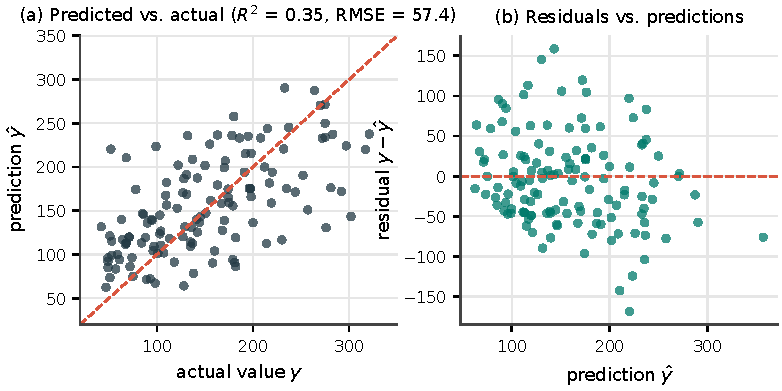
\includegraphics[width=\textwidth]{ch01/regression_diagnostics}
\caption{Diagnostic plots of a gradient boosting model on the diabetes data set (133 test
examples). (a) Predicted against actual values; (b) residuals against predictions.}
\label{fig:residuals}
\end{figure}

\subsection{Asymmetric costs}

Consider a supermarket that forecasts the demand of a product. An under-prediction causes a
\emph{stockout}: lost sales and unhappy customers. An over-prediction leaves surplus stock,
which costs storage or, for fresh products, is wasted. The two costs are rarely equal, so a
model ``centred'' on the expected demand is not the best option: the model that minimises the
MSE\index{mean squared error (MSE)} predicts the conditional mean, and the one that minimises the MAE\index{mean absolute error (MAE)} predicts the conditional
median, but neither takes the asymmetry into account. \Cref{fig:losses} compares several loss
functions.

\begin{figure}[htbp]
\centering
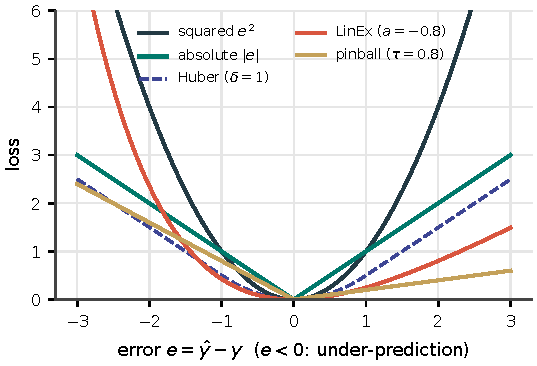
\includegraphics[width=0.72\textwidth]{ch01/regression_losses}
\caption{Loss functions as a function of the error $e=\hat y-y$. The LinEx loss with $a<0$ and
the pinball loss with $\tau>0.5$ penalise under-predictions more than over-predictions.}
\label{fig:losses}
\end{figure}

A popular asymmetric loss is the \emph{LinEx} loss \citep{zellner1986bayesian}, which is
approximately linear on one side and exponential on the other:
\begin{equation}
  L_a(e)=b\,\bigl(e^{a e}-a e-1\bigr),\qquad a\neq0,\ b>0.
\end{equation}
With $a>0$ over-predictions are penalised exponentially; with $a<0$, under-predictions. For
instance, with $a=-0.01$ and $b=1$, under-predicting the demand by 200 units costs
$L(-200)=e^{2}-3\approx4.39$, whereas over-predicting it by 200 units costs
$L(200)=e^{-2}+1\approx1.14$: being short is about four times worse than having a surplus. Note
that a function such as $1-e^{ae}$ is not a valid loss, since it is negative for errors of one
sign. With an asymmetric cost function we can select the model with the lowest average cost on
validation data or, better, train the model to minimise that cost directly.

Another important asymmetric loss is the \emph{pinball} (or quantile) loss, with
$\tau\in(0,1)$,
\begin{equation}\label{eq:pinball}
  L_\tau(y,\hat y)=\begin{cases}\tau\,(y-\hat y) & \text{if } y\geq\hat y,\\
                                 (1-\tau)\,(\hat y-y) & \text{if } y<\hat y,\end{cases}
\end{equation}
whose expected value is minimised by the $\tau$-quantile of the distribution of $y$ given $x$
\citep{koenker1978regression}. This gives a clean solution to the \emph{newsvendor problem}:
if each unit of unmet demand costs $c_u$ (underage) and each unsold unit costs $c_o$
(overage), the optimal prediction is the quantile
\begin{equation}
  \tau^\star=\frac{c_u}{c_u+c_o}.
\end{equation}
If a product has a margin of 3\EUR{} per unit sold and each unsold unit loses 1\EUR, the
forecast should target the 75th percentile of the demand, not its mean.

\begin{keyidea}
The optimal decision threshold of a classifier, $t^\star=c_{\mathrm{FP}}/(c_{\mathrm{FP}}+c_{\mathrm{FN}})$,
and the optimal quantile of a regressor, $\tau^\star=c_u/(c_u+c_o)$, have the same structure:
the costs of the two kinds of error determine the operating point\index{operating point}. A good model provides
calibrated probabilities or quantiles; the context decides how to use them.
\end{keyidea}

\subsection{Utility-based regression}

In many regression problems only some values of the target really matter: extreme rainfall,
very high returns of an investment, unusually high sales. \emph{Utility-based regression}
\citep{torgo2007utility} formalises this with a \emph{relevance function} $\phi(y)\in[0,1]$ that
marks the important values of the target, and a utility function that combines the benefits of
accurate predictions of relevant values with the costs of false alarms and missed events.
Models are then evaluated, selected and even trained to maximise utility rather than to
minimise a symmetric error. The cost penalties can also be added to standard regression
techniques so that they minimise the expected cost\index{expected cost} directly.

\subsection{Imbalanced regression}

When the values of interest are rare (extreme values of the target), regression suffers from
the same problem as imbalanced\index{class imbalance} classification: standard losses are dominated by the frequent
central values, and the model learns to ignore the extremes \citep{branco2016survey}. The
preprocessing strategies are analogous to those of classification: undersampling\index{undersampling} the common
values and oversampling\index{oversampling} the rare ones. \emph{SMOTE\index{SMOTE|textbf} for regression} (SMOTER) interpolates both
the inputs and the target between rare examples \citep{torgo2013smote}, and \emph{SMOGN}
combines random undersampling with two oversampling strategies, SMOTER and the addition of
Gaussian noise \citep{branco2017smogn}. Evaluation must then focus on the relevant values, for
example with errors restricted to them or with utility-based precision and recall, rather than
on a global MSE\index{mean squared error (MSE)}.

% ---------------------------------------------------------------------
\section{Other supervised settings}\label{sec:other}

\subsection{Ordinal regression}

In \emph{ordinal regression\index{ordinal regression|textbf}} (or ordinal classification) the classes have a natural order:
low $<$ medium $<$ high, star ratings, stages of a disease. Treating them as nominal classes
ignores that predicting \emph{high} for a \emph{low} case is worse than predicting
\emph{medium}; treating them as numbers assumes that consecutive classes are equally far
apart. Appropriate metrics \citep{gutierrez2016ordinal} include the MAE\index{mean absolute error (MAE)} computed on the ranks
of the classes, $\frac1n\sum_i|r(y_i)-r(\hat y_i)|$; rank correlations; and the
\emph{weighted kappa} \citep{cohen1968weighted},
\begin{equation}
  \kappa_w=1-\frac{\sum_{j,k}w_{jk}\,O_{jk}}{\sum_{j,k}w_{jk}\,E_{jk}},
  \qquad w_{jk}=\frac{(j-k)^2}{(c-1)^2},
\end{equation}
where $O_{jk}$ and $E_{jk}$ are the observed and the chance-expected proportions of examples
predicted as class $j$ with actual class $k$. The quadratic weights penalise distant errors
more than adjacent ones.

\subsection{Multi-label classification}

In \emph{multi-label\index{multi-label classification|textbf}} classification each example can have several non-exclusive labels
$Y_i\subseteq\mathcal L$: a news item can be about \emph{sports} and \emph{economy} at the same
time \citep{tsoumakas2007multi}. Suppose that the possible labels are \emph{sports},
\emph{politics} and \emph{economy}, that the actual labels of an example are
$\{$sports, economy$\}$ and that the predicted ones are $\{$sports, politics$\}$. Then:
\begin{itemize}
  \item the \emph{subset accuracy\index{accuracy|textbf}} (exact match) is 0, a very strict criterion;
  \item the \emph{Hamming loss}, the fraction of wrong label decisions,
        $\frac{1}{n|\mathcal L|}\sum_i|Y_i\,\triangle\,\hat Y_i|$, is $2/3$ (\emph{politics}
        wrongly added and \emph{economy} missed);
  \item the example-based \emph{Jaccard index} $|Y_i\cap\hat Y_i|/|Y_i\cup\hat Y_i|$ is $1/3$,
        and the example-based precision, recall and $F_1$ are all $1/2$;
  \item label-based metrics compute a binary metric for each label and average them with a
        micro or macro average\index{macro-average}, as in \cref{sec:crisp}.
\end{itemize}

\subsection{Hierarchical classification}

In \emph{hierarchical} classification the classes are organised in a tree or a directed acyclic
graph\index{causal graph} (animal $\to$ mammal $\to$ dog), and confusing two sibling classes is less serious than
confusing two distant ones. \emph{Hierarchical precision\index{precision|textbf} and recall\index{recall|textbf}} \citep{silla2011survey}
extend the sets of actual and predicted classes $C_i$ and $\hat C_i$ with all their ancestors
(except the root) and compute
\begin{equation}
  hP=\frac{\sum_i|\hat C_i\cap C_i|}{\sum_i|\hat C_i|},\qquad
  hR=\frac{\sum_i|\hat C_i\cap C_i|}{\sum_i|C_i|},\qquad
  hF=\frac{2\,hP\cdot hR}{hP+hR}.
\end{equation}
If a dog ($\{\text{animal},\text{mammal},\text{dog}\}$) is classified as a cat
($\{\text{animal},\text{mammal},\text{cat}\}$), $hP=hR=2/3$; if it is classified as a fish
($\{\text{animal},\text{fish}\}$), $hP=1/2$ and $hR=1/3$.

\subsection{Ranking and recommendation}

When the output of the model is an ordered list (search results, recommended products), what
matters is the quality of the first positions. Common metrics are \emph{precision\index{precision|textbf}@$k$} and
\emph{recall\index{recall|textbf}@$k$} (computed on the top $k$ items), the \emph{mean reciprocal rank\index{mean reciprocal rank|textbf}} (the average
of $1/\text{rank}$ of the first relevant item) and the \emph{normalised discounted cumulative
gain\index{NDCG|textbf}} \citep{jarvelin2002cumulated}:
\begin{equation}
  \mathrm{DCG@}k=\sum_{i=1}^{k}\frac{\mathit{rel}_i}{\log_2(i+1)},
  \qquad
  \mathrm{NDCG@}k=\frac{\mathrm{DCG@}k}{\mathrm{IDCG@}k},
\end{equation}
where $\mathit{rel}_i$ is the graded relevance of the item at position $i$ and IDCG is the DCG
of the ideal ordering. If the top three recommendations have relevances $(3,0,2)$,
$\mathrm{DCG@3}=3+0+2/2=4$; the ideal order $(3,2,0)$ gives $\mathrm{IDCG@3}=3+2/\log_2 3=4.26$,
and $\mathrm{NDCG@3}=0.94$. These metrics are studied in depth with recommender systems\index{recommender system}
(Unit~7).

\subsection{Conformal prediction}

A point prediction does not say how much we can trust it. \emph{Conformal prediction\index{conformal prediction|textbf}}
\citep{vovk2005algorithmic,angelopoulos2023conformal} is a framework for uncertainty
quantification\index{quantification} that turns any point predictor into one that outputs a \emph{set}: an interval
in regression, a set of labels in classification. These sets have a statistically valid
coverage\index{coverage} guarantee,
\begin{equation}
  P\bigl(Y_{n+1}\in\mathcal C(X_{n+1})\bigr)\geq1-\alpha,
\end{equation}
for any model and any data distribution, under the only assumption that the data are
exchangeable (for instance, independent and identically distributed). The simplest version,
\emph{split conformal\index{conformal prediction!split|textbf} prediction}, is shown in \cref{alg:conformal} and \cref{lst:conformal}.

\begin{algorithm}[htbp]
\caption{Split conformal prediction for regression}\label{alg:conformal}
\begin{algorithmic}[1]
\Require training set; calibration set $\{(x_i,y_i)\}_{i=1}^{n_{\text{cal}}}$; miscoverage level $\alpha$
\State fit a model $\hat h$ on the training set
\State compute the \emph{nonconformity scores} $s_i=|y_i-\hat h(x_i)|$ on the calibration set
\State $k\gets\lceil(n_{\text{cal}}+1)(1-\alpha)\rceil$; $\hat q\gets$ the $k$-th smallest score, or $\hat q\gets\infty$ if $k>n_{\text{cal}}$
\State \Return for each new $x$, the interval $\mathcal C(x)=\bigl[\hat h(x)-\hat q,\ \hat h(x)+\hat q\bigr]$
\end{algorithmic}
\end{algorithm}

If the required order is $n_{\text{cal}}+1$ (with 10 calibration scores and $\alpha=0.01$, for instance), the threshold is
infinite: the calibration sample cannot support a finite interval at the requested coverage without additional
assumptions.

\begin{pylisting}[label={lst:conformal}]{Split conformal prediction with a 90\% coverage target}
import numpy as np
from sklearn.ensemble import GradientBoostingRegressor

rng = np.random.default_rng(2)
X = rng.uniform(0, 10, (8000, 1))
y = X[:, 0] * np.sin(X[:, 0]) + rng.normal(0, 0.3 + 0.3 * X[:, 0])  # noisier for large x
idx = rng.permutation(len(y))
tr, cal, te = idx[:2000], idx[2000:4000], idx[4000:]   # train / calibration / test

alpha = 0.1                                           # target coverage 90%
model = GradientBoostingRegressor(random_state=0).fit(X[tr], y[tr])
scores = np.abs(y[cal] - model.predict(X[cal]))       # nonconformity scores
assert 0 < alpha < 1 and len(scores) > 0
k = int(np.ceil((len(cal) + 1) * (1 - alpha)))
q = np.inf if k > len(scores) else np.sort(scores)[k - 1]   # conformal quantile
pred = model.predict(X[te])
covered = (y[te] >= pred - q) & (y[te] <= pred + q)
print(f"q = {q:.3f};  interval width = {2 * q:.2f}")
print(f"empirical coverage = {covered.mean():.3f}  (target {1 - alpha:.2f})")
\end{pylisting}
\begin{pyoutput}
q = 3.516;  interval width = 7.03
empirical coverage = 0.903  (target 0.90)
\end{pyoutput}

The guarantee is \emph{marginal}: it holds on average over all the inputs (and over the
calibration sample, so a single run can fall slightly below $1-\alpha$). It does not hold for
every region of the input space. In \cref{fig:conformal}a the noise grows with $x$, but the
split conformal intervals have constant width: they cover 99.9\% of the test points with
$x<3$ and only 76.5\% of those with $x>7$, and the overall coverage is 90.3\%.
\emph{Conformalised quantile regression\index{conformal prediction!quantile regression|textbf}\index{quantile regression|textbf}} \citep{romano2019conformalized} starts from two quantile
regression models, trained with the pinball loss\index{pinball loss} of \cref{eq:pinball}, and conformalises their
interval; its intervals adapt to the noise (\cref{fig:conformal}b), with coverages of 93.5\%
and 91.1\% in the two regions and narrower intervals on average (6.18 against 7.03).

\begin{figure}[htbp]
\centering
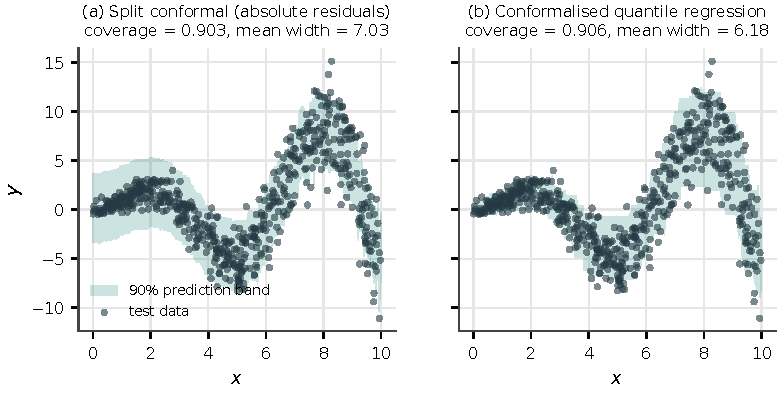
\includegraphics[width=\textwidth]{ch01/conformal}
\caption{90\% conformal prediction bands on data whose noise grows with $x$ (4000 test
points; 600 shown). (a) Split conformal with absolute residuals; (b) conformalised quantile
regression.}
\label{fig:conformal}
\end{figure}

In classification, the nonconformity score is usually $s_i=1-\hat p(y_i\mid x_i)$, and the
prediction set contains all the labels $y$ with $1-\hat p(y\mid x)\leq\hat q$: easy inputs get a
single label, ambiguous ones several. Conformal predictors are evaluated by their empirical
coverage (overall and in relevant subgroups) and by their \emph{efficiency}: at the same
coverage, narrower intervals or smaller sets are better.

\subsection{Semi-supervised learning}

In \emph{semi-supervised\index{semi-supervised learning|textbf} learning} a small amount of labelled data is combined with a large
amount of unlabelled data, which helps to discover the structure of the input space (for
instance, by placing the decision boundary in low-density regions) \citep{vanengelen2020survey}.
Evaluation must always use held-out \emph{labelled} data, and it is easy to get wrong.
\citet{oliver2018realistic} recommend comparing against well-tuned supervised baselines that
use the same model and tuning budget; using realistically small validation sets (tuning
hyperparameters with 5000 labelled validation examples makes no sense if only 250 labels are
supposed to be available); reporting performance as a function of the number of labels; and
checking what happens when the unlabelled data contain classes absent from the labelled data.

\subsection{Open-set recognition}

Standard classifiers assume a \emph{closed set}: the classes seen at test time are those seen
during training. In an \emph{open-set\index{open-set recognition|textbf}} scenario \citep{scheirer2013toward} the model may
encounter classes never seen during training: a model trained to recognise cars, dogs and
people will sooner or later receive a helicopter. A closed-set classifier is forced to assign
one of the known labels, often with high confidence (a \emph{high-confidence false
positive}). An open-set classifier must classify the known classes correctly \emph{and} reject
the unknown ones.

Two metrics are standard. The \emph{AUROC for open set} measures how well a confidence score
$S(x)$ separates known from unknown examples: known test examples are treated as positives,
unknown ones as negatives, and the usual AUC is computed (1 means perfect separation\index{fairness!separation}). It is
often complemented by the FPR\index{false positive rate} at 95\% TPR\index{true positive rate}, the fraction of unknowns accepted when 95\% of the
knowns are accepted. The \emph{open-set classification rate} (OSCR\index{open set classification rate (OSCR)}) curve
\citep{dhamija2018reducing} combines the two goals: for each threshold $\tau$ it plots the
correct classification rate on the known examples $D_K$ against the false positive rate on the
unknown examples $D_U$,
\begin{equation}
  \mathrm{CCR}(\tau)=\frac{|\{x\in D_K:\hat y(x)=y(x)\wedge S(x)\geq\tau\}|}{|D_K|},
  \qquad
  \mathrm{FPR}(\tau)=\frac{|\{x\in D_U:S(x)\geq\tau\}|}{|D_U|},
\end{equation}
and the area under it summarises the performance.

\begin{figure}[htbp]
\centering
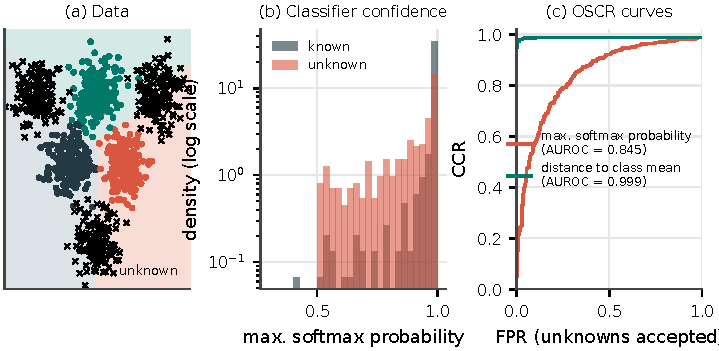
\includegraphics[width=\textwidth]{ch01/open_set}
\caption{Open-set recognition with three known classes. (a) Unknown examples (crosses) fall in
the regions of known classes. (b) The maximum softmax probability of the classifier is high
for many unknowns. (c) OSCR curves of two rejection scores.}
\label{fig:openset}
\end{figure}

In \cref{fig:openset} a logistic regression classifies the three known classes almost
perfectly (closed-set accuracy 0.988), but many unknowns receive a high confidence, and using
the maximum softmax probability to reject them gives an AUROC of only 0.845. A distance-based
score (minus the distance to the nearest class mean) separates them almost perfectly (0.999).
The main families of methods are:
\begin{itemize}
  \item \emph{confidence thresholding}: predict ``unknown'' if the highest class probability
        is below a threshold \citep{hendrycks2017baseline}. It is a simple baseline, but
        models, and deep networks in particular, are often overconfident: a network may say
        ``car: 99\%'' for an image of pure noise. ODIN \citep{liang2018enhancing} improves the
        separation with temperature scaling and small perturbations of the input;
  \item \emph{distance-based methods} (metric learning): the model maps the examples into a
        space where each class forms a compact cluster, and an example far from all clusters
        is rejected, for instance using the Mahalanobis distance \citep{lee2018simple};
  \item \emph{background class} or \emph{outlier exposure\index{outlier exposure|textbf}}: the model is trained with an
        auxiliary set of ``garbage'' examples labelled as unknown
        \citep{hendrycks2019deep}. It is very effective when the auxiliary data resemble the
        unknowns that will actually appear.
\end{itemize}

\begin{pitfall}
Open-set results depend heavily on which unknown classes are used for testing: a method that
rejects random noise easily may fail on unknowns that resemble the known classes. Always
describe the open-set protocol (known classes, unknown classes, their proportions).
\end{pitfall}

% ---------------------------------------------------------------------
\section{Evaluation in computer vision}\label{sec:vision}

\subsection{Tasks}

Computer vision distinguishes three main tasks. \emph{Image classification} assigns a single
label to a whole image (``what is in this image?'') and is evaluated with the metrics of
\cref{sec:crisp,sec:roc,sec:scoring,sec:calibration}, often with \emph{top-$k$ accuracy\index{accuracy|textbf}} (the
actual class is among the $k$ classes with the highest scores). \emph{Object detection\index{object detection|textbf}}
identifies what is in the image and \emph{where}: it draws a bounding box around each object
and labels it, as the YOLO family of detectors does \citep{redmon2016you,jocher2023yolov8}.
\emph{Image segmentation\index{segmentation|textbf}} classifies the image at the pixel level: \emph{semantic}
segmentation assigns a class to every pixel, \emph{instance} segmentation separates the
individual objects, and \emph{panoptic} segmentation does both; foundation models such as SAM
\citep{kirillov2023segment} segment arbitrary objects.

\subsection{Object detection: IoU, AP and mAP}

The \emph{intersection over union\index{intersection over union (IoU)|textbf}} (IoU, or Jaccard index) measures how well a predicted box
$B_p$ overlaps the ground-truth box $B_{gt}$:
\begin{equation}
  \mathrm{IoU}=\frac{\operatorname{area}(B_p\cap B_{gt})}{\operatorname{area}(B_p\cup B_{gt})}.
\end{equation}
An IoU of 1 is a perfect match. In \cref{fig:iou}a the boxes have areas 16 and 16 and an
intersection of 6, so $\mathrm{IoU}=6/26=0.231$. A detection counts as a true positive if it
has the same class as a ground-truth object, its IoU with it reaches a threshold (typically
0.5), and that object has not already been matched by a more confident detection; otherwise it
is a false positive (duplicates included). Ground-truth objects that are never matched are
false negatives.

\begin{figure}[htbp]
\centering
\begin{subfigure}[b]{0.46\textwidth}
\centering
\begin{tikzpicture}[scale=0.52,font=\footnotesize\sffamily]
  \draw[step=1,black!10,very thin] (0,0) grid (10,8);
  \fill[edmteal!35] (4,3) rectangle (6,6);
  \draw[edmnavy,very thick] (2,2) rectangle (6,6);
  \draw[edmcoral,very thick,dashed] (4,3) rectangle (8,7);
  \node[edmnavy,anchor=north] at (4,2) {ground truth $(2,2)$--$(6,6)$};
  \node[edmcoral,anchor=south] at (6,7) {prediction $(4,3)$--$(8,7)$};
  \node[edmteal!60!black] at (5,4.5) {$6$};
  \foreach \x in {0,2,...,10} \node[below,black!50,font=\tiny] at (\x,-0.9) {\x};
  \foreach \y in {0,2,...,8} \node[left,black!50,font=\tiny] at (0,\y) {\y};
\end{tikzpicture}
\caption{Two boxes: $\mathrm{IoU}=6/(16+16-6)=0.231$.}
\end{subfigure}\hfill
\begin{subfigure}[b]{0.46\textwidth}
\centering
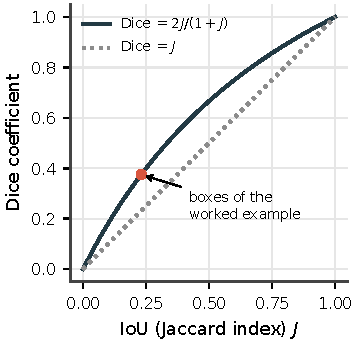
\includegraphics[width=0.9\textwidth]{ch01/dice_iou}
\caption{Dice coefficient against IoU.}
\end{subfigure}
\caption{Overlap measures. (a) Intersection over union of a predicted and a ground-truth box
(the intersection is shaded). (b) The Dice coefficient is a monotone function of the IoU and is
always at least as large.}
\label{fig:iou}
\end{figure}

Detections are sorted by confidence, and precision and recall are computed down the ranked
list. The \emph{average precision\index{average precision|textbf}\index{precision|textbf}} (AP) of a class is the area under its precision--recall
curve\index{precision--recall curve}, computed after replacing each precision by the maximum precision at any higher recall
(the \emph{interpolated} precision, which makes the curve monotone):
\begin{equation}
  \mathrm{AP}=\sum_k(r_k-r_{k-1})\,p_{\text{interp}}(r_k),\qquad
  p_{\text{interp}}(r)=\max_{r'\geq r}p(r').
\end{equation}
This all-point interpolation is used by PASCAL VOC since 2010; VOC 2007 averaged the
interpolated precision at 11 recall levels ($0,0.1,\dots,1$) and COCO uses 101 levels
\citep{everingham2010pascal,padilla2020survey}.

\begin{example}{Average precision of a detector}{ap}
A detector produces eight detections of class \emph{car}, sorted by confidence, in images that
contain five cars:
\begin{center}\small
\setlength{\tabcolsep}{5pt}
\begin{tabular}{@{}lcccccccc@{}}
\toprule
Rank & 1 & 2 & 3 & 4 & 5 & 6 & 7 & 8\\
Match (IoU $\geq0.5$) & TP & TP & FP & TP & FP & FP & TP & FP\\
Precision & 1.000 & 1.000 & 0.667 & 0.750 & 0.600 & 0.500 & 0.571 & 0.500\\
Recall & 0.2 & 0.4 & 0.4 & 0.6 & 0.6 & 0.6 & 0.8 & 0.8\\
\bottomrule
\end{tabular}
\end{center}
One car is never detected, so the maximum recall is 0.8. The interpolated precision is 1 up
to recall 0.4, $\max(0.750,0.600,0.500,0.571,0.500)=0.75$ at recall 0.6 and 0.571 at recall
0.8, so $\mathrm{AP}=0.2\cdot1+0.2\cdot1+0.2\cdot0.75+0.2\cdot0.571=0.664$
(\cref{fig:detectionpr} and \cref{lst:ap}). With the 11-point interpolation of VOC 2007, which averages the interpolated precision at the
recall levels $0,0.1,\dots,1$, the result would be approximately 0.695.
\end{example}

\begin{figure}[htbp]
\centering
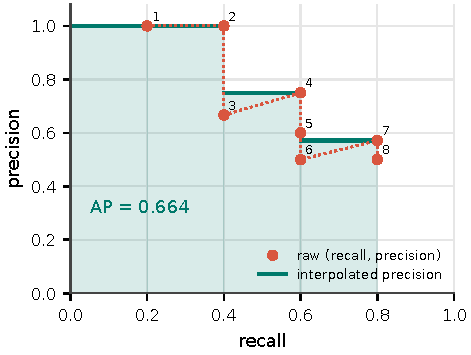
\includegraphics[width=0.56\textwidth]{ch01/detection_pr}
\caption{Precision--recall points of the detections of \cref{ex:ap} (numbered by rank),
interpolated precision and average precision (shaded area).}
\label{fig:detectionpr}
\end{figure}

\begin{pylisting}[label={lst:ap}]{IoU of two boxes and average precision of a ranked list of detections}
import numpy as np

def iou(a, b):
    """Intersection over union of two boxes given as (x1, y1, x2, y2)."""
    w = max(0, min(a[2], b[2]) - max(a[0], b[0]))
    h = max(0, min(a[3], b[3]) - max(a[1], b[1]))
    area = lambda r: (r[2] - r[0]) * (r[3] - r[1])
    return w * h / (area(a) + area(b) - w * h)

print(f"IoU = {iou((2, 2, 6, 6), (4, 3, 8, 7)):.3f}")

tp = np.array([1, 1, 0, 1, 0, 0, 1, 0])     # detections sorted by confidence
n_gt = 5                                    # number of ground-truth objects
prec = np.cumsum(tp) / np.arange(1, len(tp) + 1)
rec = np.cumsum(tp) / n_gt
env = np.maximum.accumulate(prec[::-1])[::-1]   # interpolated precision
ap = np.sum(np.diff(np.r_[0, rec]) * env)       # all-point interpolation
print("precision:", prec.round(3))
print("recall:   ", rec.round(2))
print(f"AP = {ap:.4f}")
\end{pylisting}
\begin{pyoutput}
IoU = 0.231
precision: [1.    1.    0.667 0.75  0.6   0.5   0.571 0.5  ]
recall:    [0.2 0.4 0.4 0.6 0.6 0.6 0.8 0.8]
AP = 0.6643
\end{pyoutput}

The \emph{mean average precision\index{mean average precision (mAP)|textbf}} (mAP) is the average of the AP over all classes (cars,
pedestrians, traffic lights\dots) and is the standard metric of detection benchmarks.
\emph{mAP@0.5} counts a detection as correct when its IoU exceeds 0.5 (PASCAL VOC), whereas
\emph{mAP@[0.5:0.95]} averages the mAP over IoU thresholds $0.50,0.55,\dots,0.95$ (COCO), so it
also rewards precise localisation \citep{lin2014microsoft}.

\subsection{Segmentation: pixel accuracy, mIoU and Dice}

\emph{Pixel accuracy\index{accuracy|textbf}}, the percentage of correctly classified pixels, suffers from the same
problem as accuracy with imbalanced\index{class imbalance} classes: if 90\% of an image is sky, a model that always
predicts ``sky'' reaches 90\% pixel accuracy while failing completely on the road and the cars.
The \emph{mean intersection over union\index{intersection over union (IoU)|textbf}} (mIoU) computes the IoU of each class at pixel level,
$\TP_j/(\TP_j+\FP_j+\FN_j)$, and averages it over classes \citep{long2015fully}, which prevents
large background classes from hiding errors on small but important classes such as
pedestrians.

The \emph{Dice\index{Dice coefficient|textbf} coefficient} \citep{dice1945measures} is the $F_1$ score at pixel level:
\begin{equation}
  \mathrm{Dice}=\frac{2|A\cap B|}{|A|+|B|}=\frac{2\TP}{2\TP+\FP+\FN}.
\end{equation}
It is very common in medical imaging (for instance, to segment a tumour). Dice and IoU treat
false positives and false negatives in the same, symmetric way; the difference is that Dice
counts the overlap twice, so for the same errors Dice is larger than IoU. In fact
$\mathrm{Dice}=2J/(1+J)$ with $J$ the IoU (\cref{fig:iou}b): the two boxes of \cref{fig:iou}a,
seen as masks, have $\mathrm{IoU}=0.231$ and $\mathrm{Dice}=0.375$. Being monotonically related,
they rank the segmentations\index{segmentation} of a single image identically, but their averages over many images
can rank models differently. When the shape of the boundary matters, distance-based metrics such
as the Hausdorff distance are used \citep{taha2015metrics}; \citet{maierhein2024metrics} give
detailed guidelines for choosing metrics in image analysis.

% ---------------------------------------------------------------------
\section{Evaluation in natural language processing}\label{sec:nlp}

The choice of metric in natural language processing (NLP) depends above all on whether the
model performs a \emph{classification} task (sentiment analysis, topic labelling, named entity
recognition) or a \emph{generation} task (translation, summarisation, dialogue).

\subsection{Classification and labelling tasks}

When an NLP model outputs a class (positive or negative sentiment, a topic, an intent), the
metrics of \cref{sec:crisp} apply: accuracy for balanced problems, and per-class precision,
recall and $F_1$ otherwise. In \emph{named entity recognition} most tokens belong to the
non-entity class ``O'', so token accuracy is uninformative; the standard is entity-level $F_1$,
where an entity counts as correct only if both its span and its type match exactly
\citep{tjong2003introduction}. Cohen's kappa\index{Cohen's kappa} is used to measure the agreement between human
annotators and thus the reliability of the data set.

\subsection{Text generation: n-gram overlap metrics}

Evaluating generated text is difficult because there is no single correct answer: the same
sentence can be translated or summarised in many valid ways. Traditional metrics compare the
output of the model with one or more human-written \emph{references} by counting shared
$n$-grams (sequences of $n$ words).

BLEU\index{BLEU} \citep{papineni2002bleu}, designed for machine translation, focuses on precision. For each
$n$ it computes the \emph{modified} $n$-gram precision $p_n$, in which each $n$-gram of the
candidate is counted at most as many times as it appears in the reference, and combines them
with a geometric mean and a \emph{brevity penalty} BP that prevents very short candidates from
obtaining high precision:
\begin{equation}
  \mathrm{BLEU}=\mathrm{BP}\cdot\exp\Bigl(\sum_{n=1}^{N}w_n\log p_n\Bigr),
  \qquad
  \mathrm{BP}=\begin{cases}1 & \text{if } \ell_c>\ell_r,\\ e^{1-\ell_r/\ell_c} & \text{otherwise,}\end{cases}
\end{equation}
where $\ell_c$ and $\ell_r$ are the lengths of the candidate and the reference, and usually
$N=4$ and $w_n=1/4$.

\begin{example}{BLEU and ROUGE by hand}{bleu}
Let the reference be ``\emph{the cat is on the mat}''. Candidate A, ``\emph{the cat sat on the
mat}'', has modified precisions $p_1=5/6$, $p_2=3/5$ (\emph{the cat}, \emph{on the},
\emph{the mat}), $p_3=1/4$ and $p_4=0$, and the same length as the reference. Its BLEU-4 is 0,
because one of the precisions is zero: at sentence level BLEU needs smoothing
\citep{chen2014systematic}, and it was designed to be computed over a whole corpus. Its BLEU-2
(only unigrams and bigrams) is $\sqrt{5/6\cdot3/5}=0.707$.

Candidate B, ``\emph{the feline is on the rug}'', means exactly the same as the reference but
uses synonyms: $p_1=4/6$, $p_2=2/5$ and BLEU-2 $=\sqrt{4/6\cdot2/5}=0.516$. BLEU does not
understand synonyms. Its ROUGE\index{ROUGE}-1 recall is also $4/6=0.667$, and the longest common subsequence
with the reference, ``\emph{the is on the}'', has four words, so ROUGE-L recall and precision
are $4/6$ as well.
\end{example}

Several metrics address the limitations of BLEU:
\begin{itemize}
  \item METEOR\index{METEOR} \citep{banerjee2005meteor} aligns the words of candidate and reference using
        exact matches, stems (\emph{running} matches \emph{run}) and synonyms from WordNet,
        combines precision and recall (weighting recall more) and penalises differences in word
        order;
  \item ROUGE \citep{lin2004rouge}, designed for summarisation, focuses on recall: ROUGE-N is
        the fraction of the reference $n$-grams that appear in the candidate (how much of the
        reference summary the model captured), and ROUGE-L is based on the longest common
        subsequence;
  \item chrF \citep{popovic2015chrf} computes an F-score\index{F1 score@$F_1$ score} over character $n$-grams, which is
        more robust to morphology.
\end{itemize}

\subsection{Embedding-based and learned metrics}

Modern metrics use neural representations to check whether the \emph{meaning} is the same, even
when the words differ. BERTScore\index{BERTScore} \citep{zhang2020bertscore} represents each token of the
candidate $\hat x$ and of the reference $x$ by its contextual embedding\index{embedding} and matches each token
with its most similar token in the other sentence; for instance, the recall is
\begin{equation}
  R_{\text{BERT}}=\frac{1}{|x|}\sum_{x_i\in x}\ \max_{\hat x_j\in\hat x}\ \mathbf x_i^{\top}\hat{\mathbf x}_j,
\end{equation}
with normalised embeddings, so that the inner product is the cosine\index{cosine similarity} similarity\index{similarity measure}. ``Cat'' and
``feline'' obtain a high similarity. \emph{Learned} metrics such as COMET \citep{rei2020comet} go
further and are trained to predict human quality judgements. These metrics correlate better with
human judgement than $n$-gram overlap, at the price of interpretability\index{interpretability} and of inheriting the
biases of the underlying models.

\subsection{Language models and LLMs}

A language model\index{language model} is evaluated intrinsically by its \emph{perplexity} on held-out text,
\begin{equation}
  \mathrm{PPL}=\exp\Bigl(-\frac1N\sum_{t=1}^{N}\log p(w_t\mid w_{<t})\Bigr),
\end{equation}
which is the exponential of the per-token log loss\index{log loss} of \cref{sec:scoring}. A model that assigns
probability $1/4$ to every token has perplexity 4: it is as uncertain as if it had to choose
among four equally likely words. Perplexities are only comparable for the same tokenisation and
test text.

For large language models\index{large language model (LLM)} (LLMs), traditional metrics often fail, because a correct answer may
look nothing like the reference. Common approaches are:
\begin{itemize}
  \item \emph{benchmarks} with automatically checkable answers, such as multiple-choice
        questions \citep[e.g.][]{hendrycks2021measuring}, evaluated with accuracy;
  \item \emph{functional correctness} for code: the generated program is run against unit
        tests\index{testing!unit tests}. The metric pass@$k$ is the probability that at least one of $k$ generated
        samples passes; with $n\geq k$ samples of which $c$ pass, an unbiased estimator is
        $1-\binom{n-c}{k}\big/\binom{n}{k}$ \citep{chen2021evaluating}. With $n=10$ and $c=3$,
        pass@1 $=0.3$ and pass@5 $=1-21/252=0.917$;
  \item \emph{LLM-as-a-judge\index{LLM-as-a-judge|textbf}} \citep{zheng2023judging}: a stronger model grades the outputs of
        another, either scoring each answer against a rubric (``rate this answer from 1 to 5
        according to its helpfulness'') or comparing two answers. It is cheap and agrees
        reasonably well with humans, but judges have known biases: \emph{position} bias
        (preferring the first or the second answer), \emph{verbosity} bias (preferring longer
        answers) and \emph{self-enhancement} bias (preferring answers produced by
        themselves). Mitigations include swapping the order of the answers, using explicit
        rubrics or reference answers \citep{liu2023geval}, and validating the judge against a
        sample of human judgements (reporting, for instance, Cohen's kappa\index{Cohen's kappa});
  \item \emph{human preference} evaluation: platforms such as Chatbot Arena collect pairwise
        votes and aggregate them with Bradley--Terry or Elo-style models
        \citep{chiang2024chatbot}.
\end{itemize}
Finally, benchmark questions may have leaked into the enormous pre-training corpora
(\emph{data contamination\index{contamination of benchmarks|textbf}}), which inflates the scores: this is data leakage\index{data leakage}
(\cref{sec:protocols}) at the scale of the Internet. Recent or private test sets are preferable.

\subsection{Retrieval-augmented generation}

A retrieval-augmented generation\index{retrieval-augmented generation (RAG)} (RAG) system first retrieves documents relevant to a question
and then generates an answer conditioned on them. Both components must be evaluated. The
\emph{retrieval} step is evaluated with ranking metrics (recall@$k$, MRR\index{mean reciprocal rank}, NDCG\index{NDCG}) or with
\emph{context precision\index{precision|textbf}} (are the retrieved passages relevant?) and \emph{context recall\index{recall|textbf}} (do
they contain the information needed?). The \emph{generation} step is evaluated with
\emph{faithfulness\index{faithfulness|textbf}} (is every claim of the answer supported by the retrieved documents, that is,
are there no hallucinations?), \emph{answer relevance} (does the answer actually address the
question?) and, when a reference answer exists, correctness. Frameworks such as RAGAS
\citep{es2024ragas} compute these quantities with LLM\index{large language model (LLM)} judges; for instance, faithfulness is the
fraction of the statements of the answer that can be inferred from the retrieved context.

% ---------------------------------------------------------------------
\section{Evaluating unsupervised models}\label{sec:unsupervised}

\subsection{The absence of ground truth}

Unsupervised models look for patterns in the data: groups of similar examples, associations
between variables, low-dimensional structure. Evaluating them is harder than evaluating
supervised models for two reasons. First, the patterns found may not genuinely exist: $k$-means
returns $k$ clusters even when applied to uniform noise. Second, there is no ``ground truth'',
no set of reference answers on which to test hypotheses. Unsupervised models are therefore
compared by how well they fit the data (\emph{internal} evaluation), by their agreement with
external information when it is available (\emph{external} evaluation), by their stability
when the data are perturbed \citep{vonluxburg2010clustering}, and ultimately by their usefulness
for the task that motivated the analysis.

\subsection{Clustering: internal evaluation}

Internal evaluation judges a clustering\index{clustering} using only the data that were clustered. The most
popular indices reward compact and well-separated clusters.

The \emph{silhouette\index{silhouette coefficient|textbf} coefficient} \citep{rousseeuw1987silhouettes} is computed for each example
$i$ from two quantities: $a(i)$, the mean distance between $i$ and the other points of its
cluster, and $b(i)$, the mean distance between $i$ and the points of the nearest other cluster:
\begin{equation}
  s(i)=\frac{b(i)-a(i)}{\max\{a(i),b(i)\}}\in[-1,1].
\end{equation}
The coefficient of a clustering is the mean of $s(i)$ over all the examples. Values close to 1
indicate dense, well-separated clusters, values around zero indicate overlapping clusters, and
negative values suggest that examples have been assigned to the wrong cluster. \emph{Silhouette
plots} show the individual values sorted within each cluster (\cref{fig:silhouette}): with
$k=4$, the true number of groups in the data, all the clusters are thick and have high values
(mean 0.772); with $k=3$ two groups are merged (0.740); with $k=5$ one group is split into two
thin clusters with low silhouettes (0.648).

\begin{figure}[htbp]
\centering
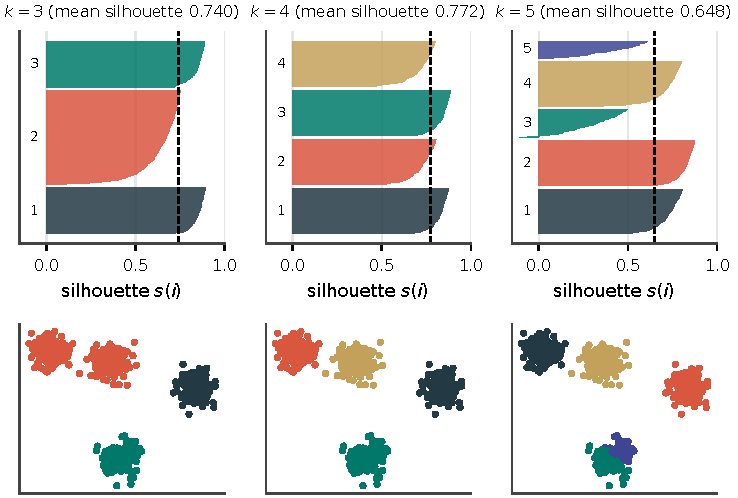
\includegraphics[width=\textwidth]{ch01/silhouette}
\caption{Silhouette plots (top) and $k$-means clusterings (bottom) of 600 points generated from
four groups, for $k=3,4,5$. The dashed line marks the mean silhouette.}
\label{fig:silhouette}
\end{figure}

The \emph{Calinski--Harabasz\index{Calinski--Harabasz index|textbf} index} (or variance ratio criterion) \citep{calinski1974dendrite}
is the ratio between the dispersion \emph{between} clusters and the dispersion \emph{within}
clusters, each normalised by its degrees of freedom:
\begin{equation}
  \mathrm{CH}=\frac{\operatorname{tr}(B_k)/(k-1)}{\operatorname{tr}(W_k)/(n-k)},
  \quad
  B_k=\sum_{q=1}^{k}n_q(\mathbf c_q-\mathbf c)(\mathbf c_q-\mathbf c)^{\top},
  \quad
  W_k=\sum_{q=1}^{k}\sum_{x\in C_q}(x-\mathbf c_q)(x-\mathbf c_q)^{\top},
\end{equation}
where $\mathbf c_q$ and $n_q$ are the centroid and size of cluster $C_q$ and $\mathbf c$ is the
global centroid; the traces are sums of squared distances. The score is higher when clusters are
dense and well separated, and it is fast to compute.

The \emph{Davies--Bouldin\index{Davies--Bouldin index|textbf} index} \citep{davies1979cluster} estimates the average similarity\index{similarity measure}
between each cluster and its most similar one, where similarity compares the distance between
clusters with their sizes:
\begin{equation}
  \mathrm{DB}=\frac1k\sum_{i=1}^{k}\max_{j\neq i}\frac{\sigma_i+\sigma_j}{d(\mathbf c_i,\mathbf c_j)},
\end{equation}
with $\sigma_i$ the mean distance of the points of cluster $i$ to its centroid. Lower values are
better (the minimum is 0). It is simpler to compute than the silhouette, but it is based on
centroids and therefore limited to Euclidean\index{Euclidean distance} distance.

In \cref{fig:indices} and \cref{lst:clustering} the three indices agree on $k=4$. In general
they do not always agree, and all of them favour convex, compact clusters: their values are generally
more favourable (higher for silhouette and Calinski--Harabasz, lower for Davies--Bouldin) for
$k$-means-like partitions than for other notions of cluster, such as the
density-based clusters found by DBSCAN, and they can be misleading for elongated or nested
shapes. The ``elbow'' of the within-cluster sum of squares is a common heuristic, and the
\emph{gap statistic} \citep{tibshirani2001estimating} compares it with what would be expected
for data without clusters.

\begin{figure}[htbp]
\centering
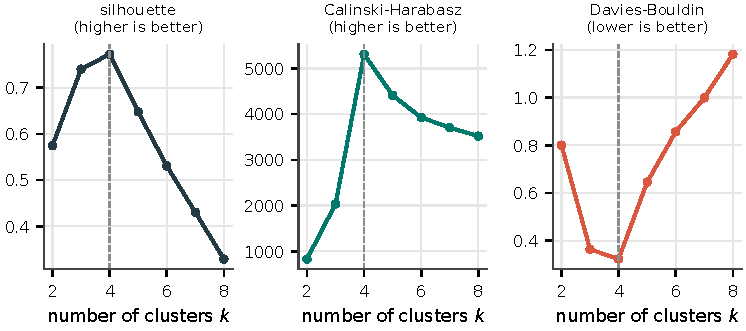
\includegraphics[width=\textwidth]{ch01/internal_indices}
\caption{Internal indices for $k$-means with $k=2,\dots,8$ on the data of \cref{fig:silhouette}.
All three point to $k=4$ (dashed lines).}
\label{fig:indices}
\end{figure}

\begin{pylisting}[label={lst:clustering}]{Internal and external indices for k-means with k = 2..6}
from sklearn.cluster import KMeans
from sklearn.datasets import make_blobs
from sklearn.metrics import (silhouette_score, calinski_harabasz_score,
                             davies_bouldin_score, adjusted_rand_score,
                             normalized_mutual_info_score)

X, y = make_blobs(n_samples=600, centers=4, cluster_std=1.2, random_state=7)
for k in range(2, 7):
    lab = KMeans(n_clusters=k, n_init=10, random_state=0).fit_predict(X)
    print(f"k={k}  sil={silhouette_score(X, lab):.3f}  "
          f"CH={calinski_harabasz_score(X, lab):6.0f}  "
          f"DB={davies_bouldin_score(X, lab):.3f}  "
          f"ARI={adjusted_rand_score(y, lab):.3f}  "
          f"NMI={normalized_mutual_info_score(y, lab):.3f}")
\end{pylisting}
\begin{pyoutput}
k=2  sil=0.574  CH=   832  DB=0.801  ARI=0.495  NMI=0.657
k=3  sil=0.740  CH=  2036  DB=0.364  ARI=0.713  NMI=0.857
k=4  sil=0.772  CH=  5309  DB=0.323  ARI=1.000  NMI=1.000
k=5  sil=0.648  CH=  4410  DB=0.646  ARI=0.918  NMI=0.944
k=6  sil=0.531  CH=  3926  DB=0.857  ARI=0.824  NMI=0.891
\end{pyoutput}

\subsection{Clustering: external evaluation}

When reference labels exist (for benchmarking, or for a labelled subset of the data), the
clustering\index{clustering} can be compared with them. Since cluster identifiers are arbitrary, the measures
must be invariant to permutations of the labels:
\begin{itemize}
  \item the \emph{Rand index} \citep{rand1971objective} is the fraction of pairs of examples
        on which both partitions agree (both together or both apart). The \emph{adjusted Rand
        index\index{adjusted Rand index|textbf}} (ARI) \citep{hubert1985comparing} corrects it for chance,
        $\mathrm{ARI}=(\mathrm{RI}-\E[\mathrm{RI}])/(\max\mathrm{RI}-\E[\mathrm{RI}])$: it is 1
        for identical partitions, close to 0 for random ones and can be negative;
  \item the \emph{mutual information} (MI) between the two labellings measures their agreement
        ignoring permutations. Its \emph{normalised} version (NMI\index{normalised mutual information}) \citep{strehl2002cluster}
        lies in $[0,1]$ and is very popular, but it is not corrected for chance and tends to
        increase with the number of clusters; the \emph{adjusted} mutual information (AMI)
        corrects it \citep{vinh2010information};
  \item \emph{homogeneity} (each cluster contains members of a single class),
        \emph{completeness} (all members of a class are assigned to the same cluster) and their
        harmonic mean, the \emph{V-measure} \citep{rosenberg2007vmeasure}, make the two kinds
        of error explicit.
\end{itemize}

\subsection{Association rules}

\emph{Association rule\index{association rules|textbf}} learning discovers interesting relations between variables in large
databases \citep{agrawal1993mining}. It identifies strong rules, ranked by some measure of
interestingness, and is used in market basket analysis, web usage mining, intrusion detection
and bioinformatics. A rule $A\Rightarrow B$ has an \emph{antecedent} $A$ and a
\emph{consequent} $B$, two disjoint sets of items. Unlike classification rules, any attribute can
appear in the consequent, and it can contain more than one attribute. \Cref{tab:baskets} shows
ten shopping baskets, and we evaluate the rule
\begin{center}
\textsc{if} sponge cakes ``Goloso'' $=1$ \textsc{and} horchata ``Xufer'' $=1$
\textsc{then} biscuits ``Trigo'' $=1$.
\end{center}

\begin{table}[htbp]
\centering\small
\caption{Ten shopping baskets (1 = the product was bought).}\label{tab:baskets}
\setlength{\tabcolsep}{4.5pt}
\begin{tabular}{@{}lccccccc@{}}
\toprule
& \makecell{Wine\\``Cabez\'on''} & \makecell{Soda\\``Chispa''} & \makecell{Wine\\``T\'io Paco''}
& \makecell{Horchata\\``Xufer''} & \makecell{Sponge cakes\\``Goloso''} & \makecell{Biscuits\\``Trigo''}
& \makecell{Chocolate\\``La Vaca''}\\
\midrule
T1  & 1 & 1 & 0 & 0 & 0 & 1 & 0\\
T2  & 0 & 1 & 1 & 0 & 0 & 0 & 0\\
T3  & 0 & 0 & 0 & 1 & 1 & 1 & 0\\
T4  & 1 & 1 & 0 & 1 & 1 & 1 & 1\\
T5  & 0 & 0 & 0 & 0 & 0 & 1 & 0\\
T6  & 1 & 0 & 0 & 0 & 0 & 1 & 1\\
T7  & 0 & 1 & 1 & 1 & 1 & 0 & 0\\
T8  & 0 & 0 & 0 & 1 & 1 & 1 & 1\\
T9  & 1 & 1 & 0 & 0 & 1 & 0 & 1\\
T10 & 0 & 1 & 0 & 0 & 1 & 0 & 0\\
\bottomrule
\end{tabular}
\end{table}

The usual measures are:
\begin{itemize}
  \item \emph{support}: how frequently the itemset $A\cup B$ (all the items of the rule) appears
        in the data. In probabilistic terms it is $P(A\cap B)$, the probability that a
        transaction contains $A$ \emph{and} $B$; some texts write $P(A\cup B)$ meaning the
        union of the \emph{itemsets}, which can be confusing. Three baskets (T3, T4, T8) contain
        the three products: absolute support 3, relative support $3/10=0.3$;
  \item \emph{confidence}: how frequently the rule is true when it can be applied,
        $P(B\mid A)=\mathrm{supp}(A\cup B)/\mathrm{supp}(A)$. Four baskets contain $A$ (T3, T4,
        T7, T8), so the confidence is $3/4=0.75$;
  \item \emph{lift\index{lift|textbf}} \citep{brin1997dynamic}: the ratio between the observed support and the
        support expected if $A$ and $B$ were independent,
        $\mathrm{conf}(A\Rightarrow B)/P(B)=P(A\cap B)/\bigl(P(A)P(B)\bigr)$. Six baskets contain
        $B$, so $\mathrm{lift}=0.3/(0.4\cdot0.6)=1.25$. A lift of 1 means independence; above 1,
        the presence of $A$ increases the probability of $B$; below 1, it decreases it;
  \item \emph{leverage}, $P(A\cap B)-P(A)P(B)=0.06$, and \emph{conviction\index{conviction|textbf}},
        $(1-P(B))/(1-\mathrm{conf})=0.4/0.25=1.6$, which is infinite for rules that are always
        true.
\end{itemize}

\begin{pylisting}[label={lst:assoc}]{Interestingness measures of an association rule}
import pandas as pd

items = ["Cabezon", "Chispa", "TioPaco", "Xufer", "Goloso", "Trigo", "LaVaca"]
T = pd.DataFrame([[1, 1, 0, 0, 0, 1, 0], [0, 1, 1, 0, 0, 0, 0], [0, 0, 0, 1, 1, 1, 0],
                  [1, 1, 0, 1, 1, 1, 1], [0, 0, 0, 0, 0, 1, 0], [1, 0, 0, 0, 0, 1, 1],
                  [0, 1, 1, 1, 1, 0, 0], [0, 0, 0, 1, 1, 1, 1], [1, 1, 0, 0, 1, 0, 1],
                  [0, 1, 0, 0, 1, 0, 0]], columns=items).astype(bool)

A = T["Goloso"] & T["Xufer"]          # antecedent: {Goloso, Xufer}
B = T["Trigo"]                        # consequent: {Trigo}
supp = (A & B).mean()
conf = supp / A.mean()
lift = conf / B.mean()
leverage = supp - A.mean() * B.mean()
conviction = (1 - B.mean()) / (1 - conf)
print(f"support={supp:.2f} confidence={conf:.2f} lift={lift:.2f} "
      f"leverage={leverage:.2f} conviction={conviction:.2f}")
\end{pylisting}
\begin{pyoutput}
support=0.30 confidence=0.75 lift=1.25 leverage=0.06 conviction=1.60
\end{pyoutput}

Two cautions apply. A high confidence can be misleading when the consequent is very frequent:
if 90\% of the baskets contain bread, a rule predicting bread with confidence 0.8 has a lift
below 1, so its antecedent actually makes bread \emph{less} likely. And when thousands of rules
are generated, many will look interesting by chance, so promising rules should be validated on
new data \citep{tan2004selecting,han2011data}.

\subsection{Other unsupervised tasks}

In \emph{anomaly detection} \citep{chandola2009anomaly}, if some labelled anomalies are
available the problem is evaluated as an extremely imbalanced\index{class imbalance} classification problem (AUC,
average precision\index{average precision}, precision@$k$ among the top-ranked cases); otherwise, experts review the
top-ranked anomalies. \emph{Dimensionality reduction} can be evaluated by the reconstruction
error, by how well neighbourhoods are preserved, or by the performance of a downstream model.
Density estimators and generative models are evaluated by the log-likelihood of held-out data,
the log loss\index{log loss} once again.

% ---------------------------------------------------------------------
\section{Comparing models statistically}\label{sec:stats}

Every performance estimate is a random variable: a different test set or a different partition
in cross-validation would give a different number. Before concluding that model A is better than
model B, we must ask whether the difference could be due to chance.

\subsection{Uncertainty of a single estimate}

If a classifier is tested on $n$ independent examples, the number of correct predictions follows
a binomial distribution. The \emph{Wilson\index{Wilson interval|textbf} interval} \citep{wilson1927probable} for the accuracy
$\hat p$ behaves better than the usual normal approximation $\hat p\pm z\sqrt{\hat p(1-\hat p)/n}$,
especially for small $n$ or accuracies close to 1:
\begin{equation}
  \frac{\hat p+\frac{z^2}{2n}\pm z\sqrt{\frac{\hat p(1-\hat p)}{n}+\frac{z^2}{4n^2}}}{1+\frac{z^2}{n}},
\end{equation}
with $z=1.96$ for 95\% confidence. An accuracy of 170/200 has the interval $[0.794, 0.893]$. For
metrics without a simple sampling distribution (AUC, $F_1$, MCC\index{Matthews correlation coefficient}\dots) the \emph{bootstrap\index{bootstrap|textbf}}
\citep{efron1993introduction} is the general solution: resample the test set with replacement
many times, recompute the metric on each resample and take the percentiles of the results
(\cref{lst:ci}).

\begin{pylisting}[label={lst:ci}]{Wilson interval for accuracy and bootstrap interval for the AUC}
import numpy as np
from scipy.stats import norm
from sklearn.metrics import roc_auc_score

def wilson_ci(k, n, conf=0.95):
    """Wilson score interval for a proportion (e.g. accuracy = k/n)."""
    z, p = norm.ppf(0.5 + conf / 2), k / n
    centre = (p + z**2 / (2 * n)) / (1 + z**2 / n)
    half = z * np.sqrt(p * (1 - p) / n + z**2 / (4 * n**2)) / (1 + z**2 / n)
    return centre - half, centre + half

def bootstrap_ci(metric, y, s, B=2000, conf=0.95, seed=0):
    """Percentile bootstrap interval for any metric(y, s)."""
    rng, stats = np.random.default_rng(seed), []
    while len(stats) < B:
        i = rng.integers(0, len(y), len(y))
        if y[i].min() != y[i].max():          # the resample needs both classes
            stats.append(metric(y[i], s[i]))
    return np.quantile(stats, [(1 - conf) / 2, (1 + conf) / 2])

print("accuracy 170/200 = 0.850, 95%% Wilson CI: [%.3f, %.3f]" % wilson_ci(170, 200))
rng = np.random.default_rng(1)
y = np.r_[np.ones(60), np.zeros(140)]
s = np.r_[rng.normal(1.2, 1, 60), rng.normal(0, 1, 140)]
lo, hi = bootstrap_ci(roc_auc_score, y, s)
print(f"AUC = {roc_auc_score(y, s):.3f}, 95% bootstrap CI: [{lo:.3f}, {hi:.3f}]")
\end{pylisting}
\begin{pyoutput}
accuracy 170/200 = 0.850, 95% Wilson CI: [0.794, 0.893]
AUC = 0.843, 95% bootstrap CI: [0.779, 0.898]
\end{pyoutput}

\subsection{Two models on the same data}

When two classifiers are evaluated on the same test set, their errors are paired. \emph{McNemar\index{McNemar's test|textbf}'s
test} \citep{mcnemar1947note} uses only the examples on which they disagree: $b$, the number
correctly classified by A and misclassified by B, and $c$, the number misclassified by A and
correctly classified by B. If both models have the same error rate\index{error rate}, $b$ should follow a binomial
distribution $\mathrm{Bin}(b+c,1/2)$, which gives an exact test; for large counts,
$\chi^2=(|b-c|-1)^2/(b+c)$ with one degree of freedom is used. \citet{dietterich1998approximate}
recommends this test when the models can be trained only once.

With cross-validation, the tempting approach is a paired $t$-test on the $k$ fold differences.
It is not valid: the training sets overlap, the differences are positively correlated, the
variance is underestimated and the test finds far too many ``significant'' differences
\citep{dietterich1998approximate}. The \emph{corrected resampled\index{corrected resampled t-test@corrected resampled $t$-test|textbf} $t$-test}
\citep{nadeau2003inference} inflates the variance to account for the overlap:
\begin{equation}
  t=\frac{\bar d}{\sqrt{\Bigl(\frac1J+\frac{n_{\text{test}}}{n_{\text{train}}}\Bigr)\hat\sigma_d^2}},
\end{equation}
where $\bar d$ and $\hat\sigma_d^2$ are the mean and the variance of the $J$ differences, and
$n_{\text{test}}/n_{\text{train}}=1/(k-1)$ in $k$-fold CV. \Cref{lst:compare} compares logistic
regression and naive Bayes\index{naive Bayes}. McNemar's test finds no significant difference ($p=0.58$). Over
10$\times$10-fold CV the mean difference in accuracy is 0.015; the naive $t$-test declares it
overwhelmingly significant ($p\approx10^{-7}$), whereas the corrected test does not ($p=0.11$).

\begin{pylisting}[label={lst:compare}]{McNemar's test and the corrected resampled t-test}
import numpy as np
from scipy.stats import binomtest, t
from sklearn.datasets import make_classification
from sklearn.linear_model import LogisticRegression
from sklearn.model_selection import (RepeatedStratifiedKFold, cross_val_score,
                                     train_test_split)
from sklearn.naive_bayes import GaussianNB

X, y = make_classification(n_samples=2000, n_features=20, n_informative=5,
                           random_state=1)
A, B = LogisticRegression(max_iter=1000), GaussianNB()

# McNemar's exact test on a single test set
X_tr, X_te, y_tr, y_te = train_test_split(X, y, test_size=0.3, random_state=0)
ok_a = A.fit(X_tr, y_tr).predict(X_te) == y_te
ok_b = B.fit(X_tr, y_tr).predict(X_te) == y_te
b, c = np.sum(ok_a & ~ok_b), np.sum(~ok_a & ok_b)
print(f"McNemar: b={b}, c={c}, exact p-value = {binomtest(b, b + c).pvalue:.4f}")

# Corrected resampled t-test (Nadeau & Bengio, 2003) on 10 x 10-fold CV
cv = RepeatedStratifiedKFold(n_splits=10, n_repeats=10, random_state=0)
d = cross_val_score(A, X, y, cv=cv) - cross_val_score(B, X, y, cv=cv)
J, ratio = len(d), 1 / 9                  # n_test / n_train in 10-fold CV
t_c = d.mean() / np.sqrt((1 / J + ratio) * d.var(ddof=1))
t_naive = d.mean() / np.sqrt(d.var(ddof=1) / J)
print(f"mean difference = {d.mean():.4f}")
print(f"naive t = {t_naive:.2f} (p = {2 * t.sf(abs(t_naive), J - 1):.1e})")
print(f"corrected t = {t_c:.2f} (p = {2 * t.sf(abs(t_c), J - 1):.4f})")
\end{pylisting}
\begin{pyoutput}
McNemar: b=38, c=44, exact p-value = 0.5811
mean difference = 0.0150
naive t = 5.69 (p = 1.3e-07)
corrected t = 1.63 (p = 0.1055)
\end{pyoutput}

\subsection{Many models on many data sets}

To compare learning algorithms rather than models, they must be evaluated on many data sets.
\citet{demsar2006statistical} recommends non-parametric tests, which do not assume normality and
are not dominated by a few data sets:
\begin{itemize}
  \item for two algorithms, the \emph{Wilcoxon\index{Mann--Whitney--Wilcoxon statistic|textbf} signed-rank test} \citep{wilcoxon1945individual}
        on the differences of performance across data sets;
  \item for $k$ algorithms on $N$ data sets, the \emph{Friedman test\index{Friedman test|textbf}} \citep{friedman1937use}:
        the algorithms are ranked on each data set (1 for the best), $R_j$ is the average rank
        of algorithm $j$, and
        \begin{equation}
          \chi^2_F=\frac{12N}{k(k+1)}\Bigl[\sum_{j}R_j^2-\frac{k(k+1)^2}{4}\Bigr]
        \end{equation}
        follows approximately a $\chi^2$ distribution with $k-1$ degrees of freedom. If the
        null hypothesis is rejected, the \emph{Nemenyi\index{Nemenyi test|textbf}} post-hoc test declares two algorithms
        different if their average ranks differ by at least the \emph{critical difference\index{critical difference diagram|textbf}}
        $\mathrm{CD}=q_\alpha\sqrt{k(k+1)/(6N)}$, with $q_{0.05}=2.728$ for $k=5$.
\end{itemize}
The results are summarised in a \emph{critical difference diagram} (\cref{fig:cd}), which
places the algorithms on the axis of average ranks and joins with a bar the groups whose
differences are not significant.

\begin{figure}[htbp]
\centering
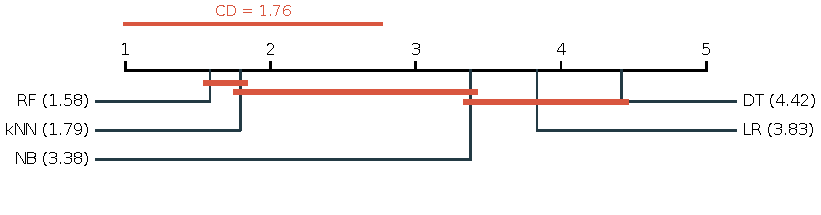
\includegraphics[width=\textwidth]{ch01/cd_diagram}
\caption{Critical difference diagram of five algorithms evaluated with the AUC (5-fold CV) on
12 synthetic data sets. Average ranks in parentheses; algorithms joined by a bar are not
significantly different (Nemenyi test, $\alpha=0.05$).}
\label{fig:cd}
\end{figure}

In the experiment of \cref{fig:cd}, logistic regression (LR), naive Bayes\index{naive Bayes} (NB), $k$-NN, a
decision tree (DT) and a random forest (RF) were compared on 12 data sets. The average ranks are
1.58 (RF), 1.79 ($k$-NN), 3.38 (NB), 3.83 (LR) and 4.42 (DT); the Friedman statistic is
$\chi^2_F=30.4$ ($p=4\times10^{-6}$) and $\mathrm{CD}=1.76$. Random forest and $k$-NN are
significantly better than logistic regression and the decision tree, and random forest is also
better than naive Bayes (difference 1.80), but $k$-NN and naive Bayes are not significantly
different (1.59). These conclusions depend on the data sets chosen: logistic regression ranks
low partly because two of the data sets (concentric circles) are not linearly separable.

Post-hoc tests on mean ranks, such as Nemenyi's, have a weakness: whether two algorithms are declared different
depends on which other algorithms take part in the comparison \citep{benavoli2016should}. When one method is the
reference (a new proposal, or the model in production), a safer analysis compares it with each of the others
using the Wilcoxon signed-rank test on the per-data-set differences \citep{wilcoxon1945individual}, with Holm's
step-down correction for the multiple comparisons \citep{holm1979simple}. Against random forest, the adjusted
$p$-values are 0.002 for LR and DT, 0.005 for NB and 0.077 for $k$-NN: the same conclusions as above, reached
without depending on the rest of the pool.

\citet{benavoli2017time} argue for \emph{Bayesian} comparisons, which give the posterior
probabilities that one algorithm is better, practically equivalent (within a \emph{region of
practical equivalence}) or worse than another: this is the question practitioners actually
want answered. With the Bayesian signed-rank test and a region of, say, $\pm0.01$ in AUC, the result is the
posterior probability of each of the three outcomes rather than a $p$-value.

\subsection{Statistical versus practical significance}

Statistical significance\index{statistical significance} is not practical significance. With a test set of a million examples a
difference of 0.1\% in accuracy can be significant and irrelevant; with 100 examples a
difference of 5\% may not be significant and yet be important. Report effect sizes with their
intervals, correct for multiple comparisons when many models are compared, and decide with the
costs and the context in mind. A model that wins on benchmark data sets may not win in your
deployment context.

% ---------------------------------------------------------------------
\section{Choosing the right metric}\label{sec:choosing}

There is no universally best metric. \Cref{tab:choosing} summarises the recommendations of this
unit, and the following questions help to design an evaluation:
\begin{enumerate}
  \item What decision will the model support: a crisp decision, a ranking or prioritisation, a
        probability estimate, a numerical forecast, a set or interval?
  \item Who bears the consequences of each kind of error, and how much do they cost?
  \item Is the operating context (class distribution, costs, capacity) known and stable, or
        uncertain and changing?
  \item Do downstream users or systems need probabilities?
  \item Which protocol gives an honest estimate: are there groups, time or space to respect, and
        is every data-dependent step inside the evaluation loop?
  \item How uncertain is the estimate, and are the differences between models significant and
        relevant?
  \item What should be monitored after deployment to detect that the context has changed
        (Unit~6)?
\end{enumerate}

\begin{table}[htbp]
\centering\small
\caption{A guide to choosing evaluation metrics.}\label{tab:choosing}
\begin{tabularx}{\textwidth}{@{}>{\raggedright\arraybackslash}p{3.7cm}>{\raggedright\arraybackslash}X>{\raggedright\arraybackslash}p{3.2cm}@{}}
\toprule
Situation & Recommended & Beware of\\
\midrule
Decisions at a known operating point & expected cost or utility; threshold $t^\star$ from calibrated probabilities & accuracy when costs are unequal\\
Unknown or changing context & ROC curve, AUC, cost curves; evaluation over ranges of contexts & a single threshold-based number\\
Rare positive class & PR curve and average precision, $F_1$/$F_\beta$, MCC, balanced accuracy & accuracy, error\\
Ranking with limited capacity & lift or gains at the operating depth, precision@$k$, NDCG, AUC & accuracy at threshold 0.5\\
Probabilities used downstream & log loss, Brier score, reliability diagram, ECE & MAE of probabilities (improper)\\
Regression, symmetric costs & MAE (robust), RMSE (large errors matter), $R^2$ with an absolute metric & $R^2$ alone; correlation\\
Regression, asymmetric costs & pinball loss, LinEx or the actual cost function & MSE-optimal (mean) predictions\\
Uncertainty quantification & coverage and interval width or set size (conformal) & intervals without coverage checks\\
Clustering & internal indices plus stability and domain validation; ARI/AMI with reference labels & a single internal index\\
\bottomrule
\end{tabularx}
\end{table}

% ---------------------------------------------------------------------
\section{Summary}\label{sec:summary}

\begin{itemize}
  \item The evaluation of learned models must be performed thoroughly, on data that played no
        role in building them; protocols must respect the structure of the data (groups,
        time) and keep every data-dependent step inside the evaluation loop.
  \item Training error is optimistic. The bias--variance\index{bias--variance trade-off} trade-off explains underfitting\index{underfitting} and
        overfitting, and learning curves\index{learning curve} help to diagnose them.
  \item Models should be validated and compared over ranges of contexts. ROC analysis\index{ROC analysis} and cost
        curves\index{cost curve} show which model is optimal for each class distribution and cost ratio.
  \item The metric must reflect the main purpose of the model: threshold metrics for decisions,
        ranking metrics for prioritisation, proper scoring rules\index{proper scoring rule} and calibration for
        probabilities.
  \item With imbalanced\index{class imbalance} classes, accuracy is misleading. Rebalancing often acts like moving the decision
        threshold and can distort the probabilities for the original population; calibrated probabilities with a cost-based
        threshold are often the better solution.
  \item Regression metrics must match the costs of the errors; asymmetric losses, quantiles and
        conformal\index{conformal prediction} intervals go beyond the mean prediction.
  \item Specialised tasks (open set\index{open-set recognition}, computer vision, natural language, clustering\index{clustering}, association
        rules\index{association rules}) have specialised metrics, but the same principles apply.
  \item Estimates are uncertain: report confidence intervals\index{confidence interval} and use valid statistical tests.
  \item Finally, we need to know the learning algorithms, their strong and weak points, to select
        the best suited ones (or adapt them) to each context.
\end{itemize}

\section*{Bibliographic notes}
\phantomsection\addcontentsline{toc}{section}{Bibliographic notes}

\citet{japkowicz2011evaluating} is the most complete textbook on the evaluation of classifiers,
and \citet{flach2012machine} offers an excellent treatment of ROC analysis\index{ROC analysis} and scoring
classifiers\index{scoring classifier}. \citet{fawcett2006introduction} remains the best tutorial introduction to ROC
analysis, and \citet{hernandez2012unified} unify most classification metrics as expected losses
under different threshold choice methods. \citet{ferri2009experimental} compare classification
metrics experimentally. \citet{raschka2018model} reviews evaluation protocols\index{evaluation protocol} and statistical
tests for machine learning, and \citet{demsar2006statistical} is the reference for comparisons
over multiple data sets. \citet{silvafilho2023classifier} survey classifier calibration,
\citet{branco2016survey} learning in imbalanced\index{class imbalance} domains, \citet{angelopoulos2023conformal}
conformal prediction\index{conformal prediction}, and \citet{maierhein2024metrics} the metrics for image analysis.

\section*{Exercises}
\phantomsection\addcontentsline{toc}{section}{Exercises}

\begin{enumerate}[label=\textbf{1.\arabic*},ref=1.\arabic*,leftmargin=*,itemsep=6pt]
  \item\label{exr:confusion} A test for a disease is applied to 200 patients, 40 of whom are
        sick. It gives 46 positive results, 30 of them for sick patients. Build the confusion
        matrix\index{confusion matrix} and compute the TPR\index{true positive rate}, TNR, PPV\index{predictive value!positive}, NPV\index{predictive value!negative}, accuracy, balanced accuracy\index{balanced accuracy}, $F_1$, MCC\index{Matthews correlation coefficient} and
        Cohen's kappa\index{Cohen's kappa}.
  \item\label{exr:ppv} The test of Exercise~\ref{exr:confusion} is used to screen a population
        with a prevalence\index{prevalence} of 2\%. What fraction of the positive results correspond to sick
        people?
  \item\label{exr:aucba} Show that the area under the ROC ``curve'' of a crisp classifier,
        formed by the points $(0,0)$, $(\FPR,\TPR)$ and $(1,1)$, equals its balanced accuracy.
  \item\label{exr:hull} Four classifiers have $(\FPR,\TPR)$ equal to A $(0.1,0.5)$,
        B $(0.2,0.7)$, C $(0.4,0.9)$ and D $(0.3,0.6)$. Draw the ROC convex hull\index{ROC convex hull}. Which
        classifier minimises the expected cost\index{expected cost} when there are 100 positives and 400 negatives,
        a false negative costs 10 and a false positive costs 1? Compute its total cost.
  \item\label{exr:roc} A ranker assigns the scores 0.9, 0.8, 0.7, 0.6, 0.55, 0.5, 0.4 and 0.3
        to eight test examples whose classes are $+,-,+,+,-,-,+,-$. Draw the ROC curve\index{ROC curve} and
        compute the AUC both as an area and by counting pairs.
  \item\label{exr:proper} Show that the expected absolute error $\E|Y-p|$ of a probability $p$
        for a binary event with true probability $q$ is minimised by $p\in\{0,1\}$. What does
        this imply for a model trained to minimise the MAE\index{mean absolute error (MAE)} of its probabilities?
  \item\label{exr:calib} A model predicts $\hat p=0.8$ for 50 test examples, 30 of which are
        positive, and $\hat p=0.3$ for 100 examples, 40 of which are positive. Compute the ECE\index{calibration!expected calibration error}
        with these two bins, and the three terms of Murphy's decomposition of the Brier score\index{Brier score}
        (\cref{eq:murphy}). Check that they add up to the Brier score.
  \item\label{exr:cost} A false positive costs 5\EUR{} and a false negative 50\EUR. Which
        threshold should be applied to calibrated probabilities? If the learner can only use
        the threshold 0.5, how should the training data be resampled?
  \item\label{exr:fraud} Using the credit card benefit matrix\index{benefit matrix} of \cref{sec:costs}, compute the
        probability of fraud above which a transaction of 50\EUR{} should be refused.
  \item\label{exr:corr} For $y=(1,2,3,4,5)$ and the predictions $\hat y=2y$, compute the Pearson\index{Pearson correlation}
        correlation, the MAE and $R^2$. Discuss.
  \item\label{exr:bakery} A bakery earns 1.20\EUR{} for each loaf sold and loses 0.40\EUR{} for
        each unsold loaf. Which quantile of the demand should its forecasting model predict?
  \item\label{exr:ap} A detector produces five detections, in order of confidence TP, FP, TP,
        TP, FP, in images with four ground-truth objects. Compute the all-point average
        precision\index{average precision}.
  \item\label{exr:bleu} Compute BLEU\index{BLEU}-2 and ROUGE\index{ROUGE}-1 recall for the candidate ``\emph{a cat is on
        the mat}'' against the reference ``\emph{the cat is on the mat}''.
  \item\label{exr:rule} Using \cref{tab:baskets}, compute the support, confidence and lift\index{lift} of
        the rule $\{$La Vaca$\}\Rightarrow\{$Cabez\'on$\}$.
  \item\label{exr:mcnemar} Two classifiers are tested on the same 500 examples. Classifier A is
        right and B wrong on 15 examples, and the opposite happens on 5. Is the difference
        significant at the 5\% level?
  \item\label{exr:protocol} A retail chain wants to predict next month's sales of each of its
        500 stores using three years of monthly data, and to tune the hyperparameters of a
        gradient boosting\index{gradient boosting} model. Design an evaluation protocol\index{evaluation protocol} that gives an honest estimate of
        the error and avoids leakage\index{data leakage}.
\end{enumerate}

\section*{Solutions to selected exercises}
\phantomsection\addcontentsline{toc}{section}{Solutions to selected exercises}

\begin{description}[font=\bfseries,leftmargin=0pt,itemsep=5pt]
  \item[\ref{exr:confusion}] $\TP=30$, $\FP=16$, $\FN=10$, $\TN=144$. $\TPR=0.75$,
        $\TNR=0.90$, $\PPV=30/46=0.652$, $\NPV=144/154=0.935$, accuracy $174/200=0.87$, balanced
        accuracy\index{balanced accuracy} $0.825$, $F_1=60/86=0.698$,
        $\mathrm{MCC}=(30\cdot144-16\cdot10)/\sqrt{46\cdot40\cdot160\cdot154}=0.618$. For kappa,
        $p_e=0.23\cdot0.20+0.77\cdot0.80=0.662$ and $\kappa=(0.87-0.662)/(1-0.662)=0.615$.
  \item[\ref{exr:ppv}] By \cref{eq:ppv}, $\PPV=0.75\cdot0.02/(0.75\cdot0.02+0.10\cdot0.98)=0.133$:
        only about one positive result in eight is a sick person.
  \item[\ref{exr:aucba}] The area is a triangle plus a trapezoid:
        $\frac12\FPR\cdot\TPR+\frac12(1-\FPR)(\TPR+1)=\frac12(1+\TPR-\FPR)=\frac12(\TPR+\TNR)$.
  \item[\ref{exr:hull}] The hull is $(0,0)\to$A$\to$B$\to$C$\to(1,1)$, with slopes 5, 2, 1 and
        $1/6$; D lies below it. The iso-cost slope is $m=(400\cdot1)/(100\cdot10)=0.4$, between
        1 and $1/6$, so C is optimal: $10$ false negatives and $160$ false positives, total cost
        $10\cdot10+160=260$ (B costs 380, A 540 and AlwaysPos 400).
  \item[\ref{exr:roc}] $P=N=4$. The positives with scores 0.9, 0.7, 0.6 and 0.4 are above 4, 3, 3
        and 1 negatives respectively, so $\mathrm{AUC}=11/16=0.6875$.
  \item[\ref{exr:proper}] $\E|Y-p|=q(1-p)+(1-q)p=q+p(1-2q)$ is linear in $p$, so its minimum over
        $[0,1]$ is at $p=1$ if $q>1/2$ and at $p=0$ if $q<1/2$. A model trained to minimise the
        MAE\index{mean absolute error (MAE)} of its probabilities learns to output (almost) crisp predictions: the MAE is not a
        proper scoring rule\index{proper scoring rule}.
  \item[\ref{exr:calib}] Bin 1: $\bar y=0.6$; bin 2: $\bar y=0.4$; overall $\bar y=70/150=0.467$.
        $\mathrm{ECE}=\frac{50}{150}0.2+\frac{100}{150}0.1=0.133$. Reliability
        $=(50\cdot0.04+100\cdot0.01)/150=0.020$; resolution
        $=(50\cdot0.133^2+100\cdot0.067^2)/150=0.0089$; uncertainty $=0.467\cdot0.533=0.249$. The
        Brier score\index{Brier score} is $0.020-0.009+0.249=0.260$, which matches the direct computation
        $(30\cdot0.04+20\cdot0.64+40\cdot0.49+60\cdot0.09)/150=39/150=0.26$.
  \item[\ref{exr:cost}] $t^\star=5/(5+50)=0.091$. Multiply the number of negatives by
        $c_{\mathrm{FP}}/c_{\mathrm{FN}}=0.1$ (keep one in ten), or replicate each positive ten
        times.
  \item[\ref{exr:fraud}] $(0.02\cdot50+20)/(1.02\cdot50+40)=21/91=0.231$.
  \item[\ref{exr:corr}] The correlation is 1, but the MAE is 3 and
        $R^2=1-55/10=-4.5$: the predictions follow the trend perfectly and are useless as
        estimates. Correlation does not measure accuracy.
  \item[\ref{exr:bakery}] $\tau^\star=1.20/(1.20+0.40)=0.75$: the 75th percentile.
  \item[\ref{exr:ap}] Precision $(1, 0.5, 0.667, 0.75, 0.6)$, recall $(0.25, 0.25, 0.5, 0.75,
        0.75)$. Interpolated precision: 1 at recall 0.25, 0.75 at 0.5 and at 0.75, so
        $\mathrm{AP}=0.25\cdot1+0.25\cdot0.75+0.25\cdot0.75=0.625$.
  \item[\ref{exr:bleu}] $p_1=5/6$ (\emph{a} does not match; \emph{the} is matched once),
        $p_2=4/5$, equal lengths, so BLEU\index{BLEU}-2 $=\sqrt{5/6\cdot4/5}=0.816$. ROUGE\index{ROUGE}-1 recall $=5/6=0.833$.
  \item[\ref{exr:rule}] La Vaca appears in T4, T6, T8 and T9, and Cabez\'on in T1, T4, T6 and
        T9; both in T4, T6 and T9. Support $0.3$, confidence $3/4=0.75$, lift\index{lift} $0.75/0.4=1.875$.
  \item[\ref{exr:mcnemar}] $b=15$, $c=5$. The exact binomial test gives $p=0.041$ and the
        $\chi^2$ test with continuity correction $\chi^2=81/20=4.05$, $p=0.044$: significant at
        the 5\% level (but not at 1\%).
  \item[\ref{exr:protocol}] One possible design: keep the last months as a final test period;
        use rolling-origin evaluation (train on months $1,\dots,t$, predict month $t+1$, for
        several $t$) for model selection, nested inside each outer split; compute every
        feature (lags, moving averages, store-level encodings) using only data available at
        prediction time; split by time rather than at random, and also check performance on
        stores held out entirely if the model will be used for new stores.
\end{description}


% =====================================================================
%  Unit 2 -- Hybrid models
%  (this file is assembled from src/ch02/*.tex by build_chapter.py)
% =====================================================================
\chapter{Hybrid Models}\label{ch:hybrid}

In September 2009, after three years of competition, Netflix\index{Netflix Prize} awarded its prize of one million dollars to a team
whose final predictions blended those of hundreds of models, combined by yet another model; combining had been the
key to every stage of the competition. And yet Netflix never put the winning blend into production: its engineers
explained that the additional accuracy\index{accuracy} did not justify the engineering effort it would have required, although they
did adopt two of the individual methods found in an earlier stage of the competition \citep{amatriain2012netflix}.
The story contains both the promise of this unit and its price.

Every learning algorithm makes assumptions, and every model makes mistakes. Instead of
searching for the single best model, we can build several and combine them. This simple
idea, often summarised as the \emph{wisdom of crowds\index{wisdom of crowds|textbf}}, is behind some of the most successful
methods of machine learning: random forests\index{random forest} and gradient boosting\index{gradient boosting}\index{boosting} dominate tabular data,
and combinations of models win most data science competitions. This unit studies how to
combine models: why combinations work, how to obtain models that are worth combining, how
to fuse their predictions, how to combine models built with different techniques, and how
to build models that know when \emph{not} to predict. We close with the price to pay:
combinations of models are harder to understand, more expensive to run, and need all the
attributes of every example.

\begin{objectives}
After studying this unit you should be able to:
\begin{itemize}
  \item explain the theoretical background that supports the combination of models
        (Condorcet\index{Condorcet's jury theorem}'s theorem, the ambiguity decomposition\index{ambiguity decomposition}, the reasons why ensembles\index{ensemble} work);
  \item distinguish the mechanisms for generating diverse models, and measure diversity\index{diversity};
  \item describe and apply the main fusion\index{fusion of models} methods (linear and product combiners\index{product combiner}, voting\index{voting},
        Bayesian model averaging\index{Bayesian model averaging}, metalearning\index{metalearning});
  \item explain and use bagging\index{bagging}, boosting, randomisation\index{randomisation}, random forests and gradient
        boosting, and know when each is preferable;
  \item combine models built with different techniques (voting, stacking\index{stacking}, cascading\index{cascading},
        mixtures of experts\index{mixture of experts});
  \item decide when a model should abstain\index{abstention} or delegate\index{delegation}: derive optimal reject rules from costs,
        evaluate cautious classifiers\index{cautious classifier}, and design delegating classifiers and cascades;
  \item know the main drawbacks of ensembles and the techniques to mitigate them, such as
        pruning and mimetic\index{mimetic classifier} models.
\end{itemize}
\end{objectives}

% ---------------------------------------------------------------------
\section{The wisdom of crowds}\label{sec:crowds}

In 1906 the statistician Francis Galton visited a livestock fair where visitors could pay a
small fee to guess the weight of an ox once slaughtered and dressed. Galton obtained the list
of estimates, and found that the middle value of the distribution, the \emph{median}, was
within one per cent of the true weight \citep{galton1907vox}: the ``vox populi'' was far
more accurate than most individual guesses. The
mean of the estimates, computed later from the same data, was even closer. The phenomenon was
popularised a century later as the \emph{wisdom of crowds\index{wisdom of crowds|textbf}} \citep{surowiecki2004wisdom}.
Crowds are wise only under certain conditions: their members must hold diverse opinions,
form them independently, and there must be a good way of aggregating them.

The same principle underlies ensemble learning. Every model has limitations and makes errors;
the aim of combining models is to manage their strengths and weaknesses so that the errors of
some are compensated by the others. Theoretical and empirical results have shown that a
combination can significantly exceed the performance of its best member.

\subsection{Condorcet's jury theorem}

The oldest formal argument in favour of combining opinions is due to the Marquis de Condorcet\index{Condorcet's jury theorem}
(1785). Suppose that $T$ voters (with $T$ odd) decide between two options by majority, that each
voter is right with probability $p$, and that they vote \emph{independently}. The number of
correct votes is then binomial, and the majority is right with probability
\begin{equation}\label{eq:condorcet}
  P_{\text{maj}}(T,p)=\sum_{k=(T+1)/2}^{T}\binom{T}{k}p^k(1-p)^{T-k}.
\end{equation}
If $p>1/2$, $P_{\text{maj}}$ grows with $T$ and tends to 1; if $p<1/2$, it decreases and tends to 0
(\cref{lst:condorcet}). A crowd of independent, better-than-random voters is almost
infallible; a crowd of worse-than-random voters is reliably wrong.

\begin{pylisting}[label={lst:condorcet}]{Accuracy of the majority vote of T independent voters}
from scipy.stats import binom

def majority_accuracy(T, p):
    """P(more than half of T independent voters are right), for odd T."""
    return binom.sf(T // 2, T, p)

sizes = (1, 5, 11, 51, 101)
for p in (0.45, 0.6, 0.7):
    accs = [f"T={T}: {majority_accuracy(T, p):.3f}" for T in sizes]
    print(f"p={p:.2f}  " + "  ".join(accs))
\end{pylisting}
\begin{pyoutput}
p=0.45  T=1: 0.450  T=5: 0.407  T=11: 0.367  T=51: 0.236  T=101: 0.156
p=0.60  T=1: 0.600  T=5: 0.683  T=11: 0.753  T=51: 0.926  T=101: 0.979
p=0.70  T=1: 0.700  T=5: 0.837  T=11: 0.922  T=51: 0.999  T=101: 1.000
\end{pyoutput}

The key assumption is independence. If the voters make correlated mistakes the benefit
shrinks. In a simple model in which, with probability $\rho$, all the voters copy a common
opinion (right with probability $p$) and otherwise vote independently, the majority is right
with probability $\rho\,p+(1-\rho)\,P_{\text{maj}}(T,p)$. With $\rho=0.3$ and $p=0.6$ the accuracy
can never exceed $0.3\cdot0.6+0.7=0.88$, however large the crowd (\cref{fig:condorcet}).

\begin{figure}[htbp]
\centering
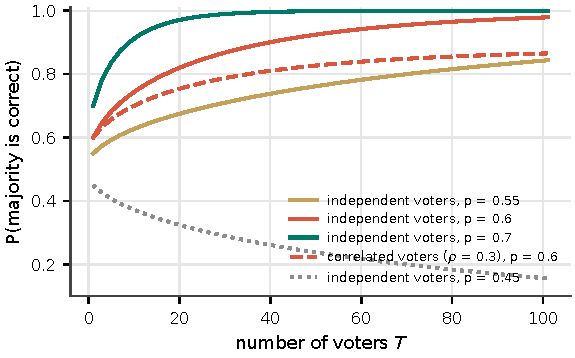
\includegraphics[width=0.74\textwidth]{ch02/condorcet}
\caption{Accuracy of a majority vote as a function of the number of voters. Independent voters
with $p>1/2$ approach perfect accuracy; correlated voters saturate; voters worse than random
($p=0.45$) get worse as the crowd grows.}
\label{fig:condorcet}
\end{figure}

For classifiers the lesson is direct. Given three models $\{h_1,h_2,h_3\}$ and a new example
$x$: if the classifiers are \emph{similar} and $h_1(x)$ is wrong, then $h_2(x)$ and $h_3(x)$ are
probably wrong too, and combining them is useless. If they are \emph{diverse}, when $h_1(x)$ is
wrong $h_2(x)$ and $h_3(x)$ may be correct, and so is the combined prediction. Combining
requires members that are both \emph{accurate} (better than random) and \emph{diverse}.

\subsection{Why do combinations work?}

\citet{dietterich2000ensemble} identified three reasons why an ensemble can be better than any of
its members:
\begin{itemize}
  \item \emph{statistical}: with limited data, many hypotheses fit the training set\index{training set} equally
        well; averaging them reduces the risk of choosing a bad one (this is the variance
        reduction of \cref{sec:biasvariance});
  \item \emph{computational}: learning algorithms perform local searches (greedy\index{multi-armed bandit!epsilon-greedy@$\varepsilon$-greedy} splits, gradient
        descent) that can get stuck in local optima; starting from different points and
        combining the results gives a better approximation;
  \item \emph{representational}: the true function may not be representable by any hypothesis of
        the class $H$, but a combination of hypotheses of $H$ may lie outside $H$ and approximate
        it better. Combining \emph{increases the expressive power} of the hypothesis language.
\end{itemize}
\Cref{fig:boundaries} illustrates the representational argument. A decision stump\index{decision stump} can only
draw one axis-parallel line (test accuracy 0.794 on the two-moons problem), but a weighted vote
of 100 stumps built by AdaBoost\index{AdaBoost} draws a complex frontier (0.902), better than a single unpruned
tree (0.855). Bagging\index{bagging}, random forests and gradient boosting\index{gradient boosting} smooth the jagged frontier of a
single tree.

\begin{figure}[htbp]
\centering
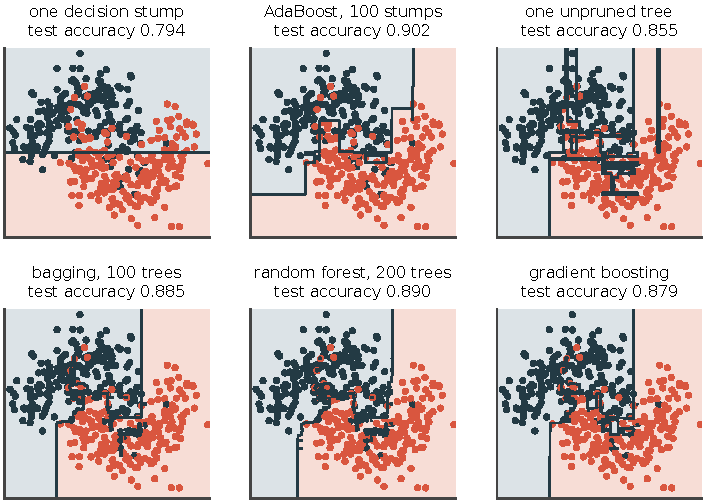
\includegraphics[width=\textwidth]{ch02/boundaries}
\caption{Decision regions on the two-moons problem (400 training examples; accuracy measured on
4000 test examples). Combinations of simple models can represent frontiers that none of their
members can.}
\label{fig:boundaries}
\end{figure}

\subsection{Diversity}

For regression with squared loss, the role of diversity\index{diversity} can be made exact. Let the ensemble
average $T$ models, $\bar f(x)=\frac1T\sum_t f_t(x)$. \citet{krogh1995neural} showed that, for any
input $x$ with target $y$,
\begin{equation}\label{eq:ambiguity}
  \underbrace{\bigl(\bar f(x)-y\bigr)^2}_{\text{ensemble error } E}
  =\underbrace{\frac1T\sum_{t=1}^{T}\bigl(f_t(x)-y\bigr)^2}_{\text{average error } \bar E}
  -\underbrace{\frac1T\sum_{t=1}^{T}\bigl(f_t(x)-\bar f(x)\bigr)^2}_{\text{ambiguity } \bar A},
\end{equation}
which follows from expanding $(f_t-y)^2=\bigl((f_t-\bar f)+(\bar f-y)\bigr)^2$ and noticing that
the deviations $f_t-\bar f$ add up to zero. The \emph{ambiguity\index{ambiguity decomposition|textbf}} $\bar A$ measures how much the
members disagree, and it is never negative: the ensemble is \emph{always} at least as good as
the average member, and it is better the more diverse the members are, provided that their
individual errors do not grow. \Cref{lst:ambiguity} checks the identity numerically for ten
bagged regression trees.

\begin{pylisting}[label={lst:ambiguity}]{The ambiguity decomposition of a bagged ensemble of regression trees}
import numpy as np
from sklearn.tree import DecisionTreeRegressor

rng = np.random.default_rng(0)
f = lambda x: np.sin(2 * np.pi * x)
X = rng.uniform(0, 1, (400, 1));     y = f(X[:, 0]) + rng.normal(0, 0.3, 400)
X_te = rng.uniform(0, 1, (2000, 1)); y_te = f(X_te[:, 0]) + rng.normal(0, 0.3, 2000)

F = []
for t in range(10):                                    # 10 trees on bootstrap samples
    i = rng.integers(0, len(y), len(y))
    F.append(DecisionTreeRegressor(max_depth=6).fit(X[i], y[i]).predict(X_te))
F = np.array(F)
f_bar = F.mean(axis=0)                                 # the ensemble prediction

E = np.mean((f_bar - y_te) ** 2)                       # error of the ensemble
E_bar = np.mean((F - y_te) ** 2)                       # average error of the members
A_bar = np.mean((F - f_bar) ** 2)                      # average ambiguity (diversity)
print(f"ensemble error        E     = {E:.4f}")
print(f"average member error  E_bar = {E_bar:.4f}")
print(f"average ambiguity     A_bar = {A_bar:.4f}")
print(f"E_bar - A_bar               = {E_bar - A_bar:.4f}")
\end{pylisting}
\begin{pyoutput}
ensemble error        E     = 0.1021
average member error  E_bar = 0.1267
average ambiguity     A_bar = 0.0247
E_bar - A_bar               = 0.1021
\end{pyoutput}

For classifiers there is no such clean decomposition, and diversity is measured with pairwise
statistics computed from the \emph{oracle outputs} of the members (correct or incorrect on each
test example) \citep{kuncheva2003measures}. For two classifiers, let $N^{11}$ be the number of
examples on which both are right, $N^{00}$ both wrong, and $N^{10}$, $N^{01}$ only one right. The
\emph{disagreement\index{diversity!disagreement|textbf}} measure and the \emph{$Q$ statistic} are
\begin{equation}
  \mathrm{dis}=\frac{N^{01}+N^{10}}{N},\qquad
  Q=\frac{N^{11}N^{00}-N^{01}N^{10}}{N^{11}N^{00}+N^{01}N^{10}},
\end{equation}
where $Q$ ranges from $-1$ to $1$ and is 0 for statistically independent classifiers. Cohen's
kappa\index{Cohen's kappa} between the predictions of two members (\cref{sec:crisp}) is another common choice. These
statistics are averaged over all pairs of members.

\begin{pylisting}[label={lst:diversity}]{Diversity and accuracy of three tree ensembles}
import numpy as np
from sklearn.datasets import make_classification
from sklearn.ensemble import (BaggingClassifier, ExtraTreesClassifier,
                              RandomForestClassifier)
from sklearn.model_selection import train_test_split
from sklearn.tree import DecisionTreeClassifier

def member_predictions(ens, X):
    feats = getattr(ens, "estimators_features_", [slice(None)] * len(ens.estimators_))
    return np.array([e.predict(X[:, f]) for e, f in zip(ens.estimators_, feats)])

def pairwise_diversity(pred, y):
    """Average disagreement and Q statistic over all pairs of members."""
    ok = pred == y                                  # correct / incorrect outputs
    dis, Q = [], []
    for i in range(len(ok)):
        for j in range(i + 1, len(ok)):
            n11, n00 = np.sum(ok[i] & ok[j]), np.sum(~ok[i] & ~ok[j])
            n10, n01 = np.sum(ok[i] & ~ok[j]), np.sum(~ok[i] & ok[j])
            dis.append((n01 + n10) / len(y))
            Q.append((n11 * n00 - n01 * n10) / (n11 * n00 + n01 * n10))
    return np.mean(dis), np.mean(Q)

X, y = make_classification(n_samples=3000, n_features=20, n_informative=10, n_redundant=4,
                           flip_y=0.05, random_state=1)
X_tr, X_te, y_tr, y_te = train_test_split(X, y, test_size=0.5, random_state=0)
ensembles = {"bagging": BaggingClassifier(DecisionTreeClassifier(), n_estimators=50,
                                          random_state=0),
             "random forest": RandomForestClassifier(50, random_state=0),
             "extra trees": ExtraTreesClassifier(50, random_state=0)}
for name, ens in ensembles.items():
    pred = member_predictions(ens.fit(X_tr, y_tr), X_te)
    dis, Q = pairwise_diversity(pred, y_te)
    print(f"{name:13s} member acc={np.mean(pred == y_te):.3f}  disagreement={dis:.3f}  "
          f"Q={Q:.3f}  ensemble acc={ens.score(X_te, y_te):.3f}")
\end{pylisting}
\begin{pyoutput}
bagging       member acc=0.803  disagreement=0.221  Q=0.659  ensemble acc=0.891
random forest member acc=0.786  disagreement=0.269  Q=0.483  ensemble acc=0.907
extra trees   member acc=0.775  disagreement=0.293  Q=0.391  ensemble acc=0.920
\end{pyoutput}

\Cref{lst:diversity} shows the typical trade-off: the members of a random forest are less
accurate than the bagged trees (0.786 against 0.803) but more diverse ($Q=0.48$ against 0.66),
and the forest is more accurate (0.907 against 0.891); extremely randomised trees\index{extra trees} push the
trade-off further. A \emph{kappa--error\index{kappa--error diagram|textbf} diagram} \citep{margineantu1997pruning} plots every pair
of members as a point (agreement, average error), and shows at a glance how each method
balances the two (\cref{fig:kappaerror}).

\begin{figure}[htbp]
\centering
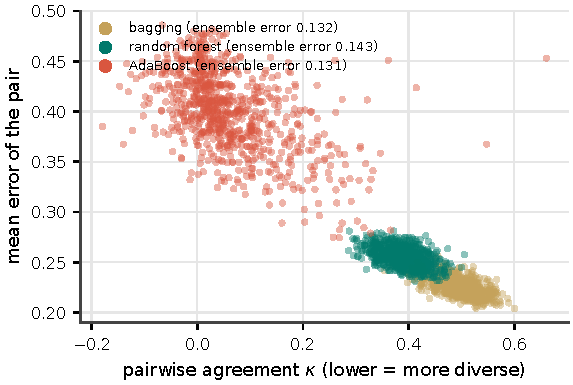
\includegraphics[width=0.74\textwidth]{ch02/kappa_error}
\caption{Kappa--error diagram of three ensembles of 40 trees. Each point is a pair of members.
Bagging produces accurate but similar members; AdaBoost produces weak but very diverse ones.}
\label{fig:kappaerror}
\end{figure}

% ---------------------------------------------------------------------
\section{Combining models}\label{sec:combining}

A combination of models has two ingredients: a way of generating a set of \emph{diverse}
models, and a way of \emph{fusing} their predictions.

\subsection{Generating diverse models}

Diverse models can be obtained by combining \emph{different learning techniques} (a neural
network, a decision tree\index{decision tree} and a nearest-neighbour\index{k-nearest neighbours@$k$-nearest neighbours} classifier), which leads to the \emph{hybrid}
methods of \cref{sec:hybrid}, or by running \emph{one learning technique} several times with
some variation, which leads to the \emph{ensemble\index{ensemble|textbf}} methods of \cref{sec:ensembles}. In the
second case, diversity\index{diversity} can be induced by:
\begin{itemize}
  \item \emph{manipulating the training examples}: each model sees a different subset or a
        different weighting of the examples (bagging\index{bagging}, boosting);
  \item \emph{manipulating the input features}: each model sees a different subset of the
        attributes, as in the random subspace method \citep{ho1998random};
  \item \emph{manipulating the classes}: the classes of the training set are modified, for
        instance by grouping them into different binary problems whose combination recovers
        the original classes, as in error-correcting output codes \citep{dietterich1995solving};
  \item \emph{injecting randomness} into the learning process: random initial weights of
        a neural network, random choices among the best splits of a tree (randomisation\index{randomisation}),
        random thresholds\index{threshold} (extremely randomised trees\index{extra trees}, \citealp{geurts2006extremely}).
\end{itemize}
\citet{brown2005diversity} distinguish \emph{implicit} diversity generation, which uses
indirect means and hopes that diversity appears (random samples, random features), from
\emph{explicit} diversity generation, which constructs each new member so that it is
substantially different from the previous ones (boosting reweights the examples the
ensemble gets wrong; Decorate\index{Decorate} adds examples that contradict it).

\subsection{Fusion methods}

Let $f_t(y\mid x)$ be the probability (or score) that model $t$ assigns to class $y$, for
$t=1,\dots,T$. The main ways of combining them are the following.

\paragraph{Linear combiner} A weighted average of the outputs,
\begin{equation}\label{eq:linear}
  \bar f(y\mid x)=\sum_{t=1}^{T}w_t\,f_t(y\mid x),
\end{equation}
applicable to regression and to soft (probabilistic) classification. With $w_t=1/T$ it is the
simple uniform average. Estimating the weights without overfitting\index{overfitting} is difficult, and in
practice the uniformly weighted average is used very often, and is hard to beat.

\paragraph{Product combiner} A (weighted) product of the probabilities,
\begin{equation}\label{eq:product}
  \bar f(y\mid x)=\frac1Z\prod_{t=1}^{T}f_t(y\mid x)^{w_t},
\end{equation}
where $Z$ is a normalisation factor that makes $\bar f$ a valid probability distribution. With non-negative
weights summing to one it is a weighted \emph{geometric mean} (a logarithmic pool); with unit exponents, as in
\cref{lst:fusion}, it is a plain normalised product, which gives sharper probabilities. If the models
use \emph{different} evidence, conditionally independent given the class, Bayes' rule gives
$P(y\mid x_1,\dots,x_T)\propto P(y)^{1-T}\prod_tP(y\mid x_t)$: multiplying posteriors counts the prior $T$ times
unless it is corrected, and calibration\index{calibration} of the members alone does not make the product optimal. The
product also has a \emph{veto} effect: a
single model that assigns a probability close to zero to a class practically eliminates it.
Again, the weights are difficult to determine. Both combiners are special cases of the
\emph{generalised mean},
\begin{equation}
  \bar f(y\mid x)=\frac1Z\Bigl(\sum_{t=1}^{T}w_t\,f_t(y\mid x)^{\alpha}\Bigr)^{1/\alpha},
\end{equation}
which, for weights summing to one, gives the linear combiner\index{linear combiner} for $\alpha=1$, the weighted geometric mean as
$\alpha\to0$, the
maximum as $\alpha\to\infty$ and the minimum as $\alpha\to-\infty$: a continuum of possible
combining strategies.

\paragraph{Voting} Each classifier votes for a class, and the class with the most votes is
selected: the \emph{majority} vote if it needs more than half of the votes, the
\emph{plurality} vote otherwise. Ties can be broken in favour of the majority class. Voting\index{voting}
works with crisp classifiers and ignores the confidence of the members. \emph{Weighted} voting
gives each member a weight, again difficult to establish.

\begin{example}{Three ways of fusing three models}{fusion}
Three models assign these probabilities to the classes A and B for an example:
$h_1=(0.90,0.10)$, $h_2=(0.45,0.55)$ and $h_3=(0.40,0.60)$. Two of the three models prefer B,
so the majority vote predicts B. The average is $(0.583,0.417)$, which predicts A: the
confident opinion of $h_1$ outweighs the two lukewarm votes for B. The normalised product is
$(0.831,0.169)$, which also predicts A (\cref{lst:fusion}). Voting counts heads; averaging
weighs confidence.
\end{example}

\begin{pylisting}[label={lst:fusion}]{Majority vote, linear combiner and product combiner}
import numpy as np

# Probabilities of the classes (A, B) given by three models to one example
P = np.array([[0.90, 0.10],
              [0.45, 0.55],
              [0.40, 0.60]])
classes = np.array(["A", "B"])

votes = np.bincount(P.argmax(axis=1), minlength=2)   # majority voting
mean = P.mean(axis=0)                                 # linear combiner (uniform)
prod = P.prod(axis=0) / P.prod(axis=0).sum()          # product combiner (normalised)
print("votes:  ", votes, "->", classes[votes.argmax()])
print("mean:   ", mean.round(3), "->", classes[mean.argmax()])
print("product:", prod.round(3), "->", classes[prod.argmax()])
\end{pylisting}
\begin{pyoutput}
votes:   [1 2] -> B
mean:    [0.583 0.417] -> A
product: [0.831 0.169] -> A
\end{pyoutput}

\paragraph{Bayesian model averaging} From a Bayesian perspective, using only one model ignores
the uncertainty of having a partial view of the problem, represented by the training data $D$.
Bayesian model averaging\index{Bayesian model averaging} (BMA) combines all the models $h$ of the hypothesis space, weighted by
their posterior probability \citep{hoeting1999bayesian}:
\begin{equation}
  P(y\mid x,D)=\sum_{h}P(y\mid x,h)\,P(h\mid D),
  \qquad
  P(h\mid D)\propto P(D\mid h)\,P(h),
\end{equation}
where $P(h)$ is the prior probability of model $h$ and $P(D\mid h)$ its likelihood. BMA propagates
the uncertainty over the candidate models; it is coherent when the model space, the priors and the
likelihood are adequate, and its behaviour depends on all of them and on the prediction objective. When
every candidate is misspecified, the posterior may concentrate on a single model as data grow, so BMA
behaves more like model \emph{selection} than like an ensemble, even when a mixture would predict better
\citep{domingos2000bayesian,yao2018using}. Cross-validated stacking\index{stacking} (\cref{sec:hybrid}) instead chooses
the weights to optimise predictive performance: the two methods answer different questions.

\paragraph{Metalearning} Instead of fixing the fusion\index{fusion of models} rule, we can \emph{learn} it: a second-level
model is trained to combine the predictions of the members. This requires extra (validation)
data, since the combiner must be trained on predictions made on examples that the members have
not seen. Stacking and cascading\index{cascading} (\cref{sec:hybrid}) are the main examples.

% ---------------------------------------------------------------------
\section{Ensemble methods}\label{sec:ensembles}

Ensemble methods generate many models with a single learning technique, most often decision
trees, and combine them. \Cref{fig:bagboost} contrasts the two classic families: bagging\index{bagging} builds
its members independently and in parallel; boosting builds them sequentially, each one focused
on the mistakes of the previous ones.

\begin{figure}[htbp]
\centering
\begin{tikzpicture}[font=\scriptsize\sffamily,
  box/.style={draw=edmnavy,fill=edmnavy!6,rounded corners=2pt,minimum width=15mm,minimum height=6mm,align=center},
  mod/.style={draw=edmteal,fill=edmteal!10,rounded corners=2pt,minimum width=13mm,minimum height=6mm,align=center},
  fus/.style={draw=edmcoral,fill=edmcoral!10,rounded corners=2pt,minimum width=14mm,minimum height=7mm,align=center},
  arr/.style={-{Stealth[length=1.8mm]},edmnavy}]
  % ---- bagging
  \node[box] (d) at (0,0) {training\\data};
  \foreach \i/\y in {1/1.1,2/0,3/-1.1}{
    \node[box,minimum width=17mm] (b\i) at (2.3,\y) {bootstrap\\sample \i};
    \node[mod] (m\i) at (4.4,\y) {model \i};
    \draw[arr] (d.east) -- (b\i.west);
    \draw[arr] (b\i) -- (m\i);
  }
  \node[fus] (v) at (6.3,0) {uniform\\vote};
  \foreach \i in {1,2,3} \draw[arr] (m\i.east) -- (v.west);
  \node[font=\small\sffamily\bfseries,text=edmnavy] at (3.2,1.9) {Bagging};
  % ---- boosting
  \begin{scope}[xshift=7.6cm]
    \foreach \i/\y in {1/1.1,2/0,3/-1.1}{
      \node[box,minimum width=17mm] (w\i) at (0.9,\y) {weighted\\data, round \i};
      \node[mod] (n\i) at (3.0,\y) {model \i\\[-1pt]$\alpha_\i$};
      \draw[arr] (w\i) -- (n\i);
    }
    \draw[arr,edmcoral] (n1.south west) -- node[left,pos=0.3,text=edmcoral] {reweight} (w2.north east);
    \draw[arr,edmcoral] (n2.south west) -- node[left,pos=0.3,text=edmcoral] {reweight} (w3.north east);
    \node[fus] (wv) at (4.9,0) {weighted\\vote};
    \foreach \i in {1,2,3} \draw[arr] (n\i.east) -- (wv.west);
    \node[font=\small\sffamily\bfseries,text=edmnavy] at (2.0,1.9) {Boosting};
  \end{scope}
\end{tikzpicture}
\caption{Bagging trains its members independently on bootstrap samples and combines them with a
uniform vote. Boosting trains them sequentially on reweighted data, increasing the weight of the
examples misclassified so far, and combines them with a weighted vote.}
\label{fig:bagboost}
\end{figure}

\subsection{Bagging}

\emph{Bagging\index{bagging|textbf}} (bootstrap\index{bootstrap} aggregating) was proposed by \citet{breiman1996bagging}. Each member of
the ensemble is learned from a different data set, a \emph{bootstrap sample} obtained by drawing
$n$ examples uniformly at random and with replacement from the $n$ training examples
(\cref{sec:protocols}); the members are combined with a uniform vote, or by averaging their
probabilities. The only parameter is the size $T$ of the ensemble.

Bagging is an implicit diversity\index{diversity} generation method, and it works because averaging reduces
variance. If the predictions of the members are identically distributed random variables with
variance $\sigma^2$ and pairwise correlation $\rho$, the variance of their average is
\citep[Section~15.2]{hastie2009elements}
\begin{equation}\label{eq:avgvar}
  \Var\Bigl(\frac1T\sum_{t=1}^{T}f_t(x)\Bigr)=\rho\,\sigma^2+\frac{1-\rho}{T}\,\sigma^2 .
\end{equation}
The second term vanishes as $T$ grows, but the first one does not: the benefit of bagging is
limited by the correlation between its members. Two practical consequences follow:
\begin{itemize}
  \item bagging works well with \emph{unstable} models, those that change a lot with small
        changes of the training data (unpruned trees, neural networks), and does little for
        stable ones ($k$-NN, linear models), whose bootstrap replicas are almost identical;
  \item about 36.8\% of the training examples are left out of each bootstrap sample, so every
        training example can be predicted by the members that did not see it. This
        \emph{out-of-bag\index{out-of-bag estimate|textbf}} (OOB) estimate gives an almost free estimate of the generalisation\index{generalisation}
        performance.
\end{itemize}
Since the members are independent, bagging is trivially parallelised.

\subsection{Boosting}

Boosting builds the ensemble sequentially. AdaBoost\index{AdaBoost} \citep{freund1996experiments,freund1997decision},
the most popular algorithm of the family, keeps a weight for each training example. In each
round a new model is trained with the current weights, the weights of the examples it
misclassifies are increased, and those of the correct ones decreased, so that the next model
focuses on the examples that the ensemble finds difficult. Each model also receives a weight
$\alpha_t$ that depends on its accuracy, and the final prediction is a weighted vote
(\cref{alg:adaboost}). The algorithm stops when a limit of $T$ models is reached or when a
model is no better than random.

\begin{algorithm}[htbp]
\caption{AdaBoost (binary classes $y\in\{-1,+1\}$)}\label{alg:adaboost}
\begin{algorithmic}[1]
\Require training set $\{(x_i,y_i)\}_{i=1}^{n}$; base learner; number of rounds $T$
\State $w_i\gets1/n$ for $i=1,\dots,n$
\For{$t=1,\dots,T$}
  \State train $h_t$ with weights $w$
  \State $\varepsilon_t\gets\sum_{i:\,h_t(x_i)\neq y_i}w_i$ \Comment{weighted error}
  \If{$\varepsilon_t=0$} \textbf{return} $h_t$ \Comment{perfect on the training data} \EndIf
  \If{$\varepsilon_t\geq1/2$} \textbf{stop} \Comment{no weak learner found} \EndIf
  \State $\alpha_t\gets\frac12\ln\frac{1-\varepsilon_t}{\varepsilon_t}$ \Comment{weight of the model}
  \State $w_i\gets w_i\,e^{\alpha_t}$ if $h_t(x_i)\neq y_i$, and $w_i\gets w_i\,e^{-\alpha_t}$ otherwise
  \State normalise $w$ so that $\sum_i w_i=1$
\EndFor
\State \Return $H(x)=\operatorname{sign}\bigl(\sum_{t}\alpha_t\,h_t(x)\bigr)$
\end{algorithmic}
\end{algorithm}

\begin{example}{One round of AdaBoost}{adaround}
Ten training examples start with weight 0.1 each, and the first model misclassifies three of
them, so $\varepsilon_1=0.3$ and $\alpha_1=\frac12\ln(0.7/0.3)=0.424$. The weights of the three
mistakes are multiplied by $e^{0.424}=1.528$ and those of the seven correct examples by
$e^{-0.424}=0.655$. After normalising, each mistake weighs $1/6$ and each correct example
$1/14$: the misclassified examples, 30\% of the data, now carry half of the total weight. In
fact, after every update the previous model has weighted error exactly 0.5, so the next model
is forced to learn something different: boosting generates diversity\index{diversity} \emph{explicitly}.
\end{example}

\Cref{lst:adaboost} implements \cref{alg:adaboost} in a few lines and obtains exactly the same
accuracy as scikit-learn's implementation: 100 decision stumps\index{decision stump} combine into a classifier with a test accuracy of 0.915. The first stump
reaches 0.781, but the later ones fit differently weighted versions of the training data, and on the
original test data\index{test set} their mean accuracy is only 0.557: a weak learner\index{weak learner} must be better than random on
the weighted data of its round, not on the original distribution.

\begin{pylisting}[label={lst:adaboost}]{AdaBoost written from scratch and compared with scikit-learn}
import numpy as np
from sklearn.datasets import make_classification
from sklearn.ensemble import AdaBoostClassifier
from sklearn.model_selection import train_test_split
from sklearn.tree import DecisionTreeClassifier

X, y01 = make_classification(n_samples=2000, n_features=10, n_informative=5,
                             random_state=4)
y = 2 * y01 - 1                                   # AdaBoost uses labels in {-1, +1}
X_tr, X_te, y_tr, y_te = train_test_split(X, y, test_size=0.5, random_state=0)

w = np.full(len(y_tr), 1 / len(y_tr))             # uniform initial weights
stumps, alphas = [], []
for t in range(100):
    h = DecisionTreeClassifier(max_depth=1).fit(X_tr, y_tr, sample_weight=w)
    miss = h.predict(X_tr) != y_tr
    eps = w[miss].sum()                           # weighted training error
    if eps == 0 or eps >= 0.5:                    # perfect, or no weak learner
        break
    alpha = 0.5 * np.log((1 - eps) / eps)         # weight of the new member
    w *= np.exp(np.where(miss, alpha, -alpha))    # mistakes gain weight
    w /= w.sum()
    stumps.append(h)
    alphas.append(alpha)
    if t < 3:
        print(f"round {t + 1}: weighted error={eps:.3f}  alpha={alpha:.3f}")

F = sum(a * h.predict(X_te) for a, h in zip(alphas, stumps))
print(f"our AdaBoost (100 stumps):  test accuracy={np.mean(np.sign(F) == y_te):.3f}")
ada = AdaBoostClassifier(DecisionTreeClassifier(max_depth=1), n_estimators=100,
                         random_state=0).fit(X_tr, y_tr)
print(f"scikit-learn's AdaBoost:    test accuracy={ada.score(X_te, y_te):.3f}")
print(f"the first stump:            test accuracy={stumps[0].score(X_te, y_te):.3f}")
mean_acc = np.mean([h.score(X_te, y_te) for h in stumps])
print(f"mean of the 100 stumps:      test accuracy={mean_acc:.3f}")
\end{pylisting}
\begin{pyoutput}
round 1: weighted error=0.219  alpha=0.636
round 2: weighted error=0.264  alpha=0.512
round 3: weighted error=0.281  alpha=0.470
our AdaBoost (100 stumps):  test accuracy=0.915
scikit-learn's AdaBoost:    test accuracy=0.915
the first stump:            test accuracy=0.781
mean of the 100 stumps:      test accuracy=0.557
\end{pyoutput}

AdaBoost has an elegant theory. Its training error is bounded by
$\prod_t2\sqrt{\varepsilon_t(1-\varepsilon_t)}$, which decreases exponentially with $T$ when every
member keeps a weighted error of at most $1/2-\gamma$ for a fixed $\gamma>0$ (a \emph{weak learner}): the
bound is then at most $e^{-2\gamma^2T}$. That is a statement about the training error; the good generalisation\index{generalisation}
of AdaBoost
has been explained in terms of the \emph{margins} of the training examples
\citep{schapire1998boosting}. AdaBoost can also be seen as a greedy\index{multi-armed bandit!epsilon-greedy@$\varepsilon$-greedy} minimisation of the
exponential loss $\sum_i e^{-y_iF(x_i)}$, with $F(x)=\sum_t\alpha_th_t(x)$
\citep{friedman2000additive}. This last view explains its main weakness: the exponential loss
grows very fast for examples with large negative margins, so mislabelled\index{label noise} examples receive
enormous weights. \emph{Boosting\index{boosting|textbf} is vulnerable to noisy data}, as we will see in
\cref{sec:performance}.

\subsection{Gradient boosting}

\emph{Gradient boosting\index{gradient boosting|textbf}\index{boosting|textbf}} \citep{friedman2001greedy} generalises the idea to any differentiable
loss $\ell$. The model is an additive expansion $F_T(x)=F_0(x)+\sum_{t=1}^{T}\nu\,h_t(x)$; at each
step, a new model $h_t$ (usually a small regression tree) is fitted to the \emph{negative
gradient} of the loss with respect to the current predictions,
\begin{equation}
  r_{it}=-\frac{\partial\,\ell\bigl(y_i,F(x_i)\bigr)}{\partial F(x_i)}\Big|_{F=F_{t-1}},
\end{equation}
which for the squared loss is simply the residual\index{residual analysis} $y_i-F_{t-1}(x_i)$: each new tree predicts the
errors of the previous ones, and its predictions are added to the ensemble. The \emph{learning
rate\index{learning rate|textbf}} (shrinkage) $\nu\in(0,1]$ slows down the learning, which improves generalisation\index{generalisation} at the
cost of more trees; the number of trees is usually chosen by \emph{early stopping\index{early stopping|textbf}} on a
validation set\index{validation set}.

Efficient implementations of gradient boosting with regularisation, histogram-based splits and
careful engineering, such as XGBoost\index{XGBoost} \citep{chen2016xgboost}, LightGBM \citep{ke2017lightgbm} and
CatBoost \citep{prokhorenkova2018catboost}, have dominated applied machine learning on
\emph{tabular} data and data science competitions for a decade. scikit-learn's
\code{HistGradientBoostingClassifier} follows the same design (\cref{lst:gb}).

\begin{pylisting}[label={lst:gb}]{Random forest, gradient boosting and histogram gradient boosting with early stopping}
from sklearn.datasets import make_classification
from sklearn.ensemble import (GradientBoostingClassifier, HistGradientBoostingClassifier,
                              RandomForestClassifier)
from sklearn.metrics import roc_auc_score
from sklearn.model_selection import train_test_split

X, y = make_classification(n_samples=20000, n_features=30, n_informative=12, n_redundant=6,
                           flip_y=0.05, class_sep=0.8, random_state=2)
X_tr, X_te, y_tr, y_te = train_test_split(X, y, test_size=0.5, random_state=0)
models = {
    "random forest (300 trees)": RandomForestClassifier(300, n_jobs=-1, random_state=0),
    "gradient boosting (300 trees)": GradientBoostingClassifier(n_estimators=300,
                                                                random_state=0),
    "histogram GB + early stopping": HistGradientBoostingClassifier(
        max_iter=2000, early_stopping=True, n_iter_no_change=30, random_state=0)}
for name, m in models.items():
    auc = roc_auc_score(y_te, m.fit(X_tr, y_tr).predict_proba(X_te)[:, 1])
    used = f"   (trees used: {m.n_iter_})" if hasattr(m, "n_iter_") else ""
    print(f"{name:30s} AUC={auc:.4f}{used}")
\end{pylisting}
\begin{pyoutput}
random forest (300 trees)      AUC=0.9682
gradient boosting (300 trees)  AUC=0.9631
histogram GB + early stopping  AUC=0.9687   (trees used: 224)
\end{pyoutput}

\subsection{Bagging versus boosting}

\Cref{tab:bagboost} summarises the main differences. Boosting usually obtains better accuracy
with clean data, while bagging\index{bagging} is more robust in noisy contexts and easier to parallelise.

\begin{table}[htbp]
\centering\small
\caption{Bagging and AdaBoost compared. Gradient boosting is also sequential, but it fits
pseudo-residuals, adds up the contributions of its members, and its sensitivity to noise depends on
the loss.}\label{tab:bagboost}
\begin{tabularx}{\textwidth}{@{}>{\raggedright\arraybackslash}p{3.2cm}XX@{}}
\toprule
& Bagging & AdaBoost\\
\midrule
Training data of each member & bootstrap sample & all data, reweighted (or resampled)\\
Construction & independent, parallel & sequential\\
Diversity & implicit & explicit (focus on the mistakes)\\
Fusion & unweighted (uniform) vote or average & weighted vote ($\alpha_t$)\\
Number of members & always $T$ & $T$ is a limit; may stop earlier\\
Main effect & reduces variance & reduces bias (and variance)\\
Best base models & unstable, low bias (deep trees) & weak learners (stumps, small trees)\\
Accuracy & good & usually better\\
Label noise & robust in many problems & sensitive (exponential loss)\\
\bottomrule
\end{tabularx}
\end{table}

\subsection{Randomisation}

\citet{dietterich2000experimental} proposed a very simple way of generating diverse decision
trees: \emph{randomisation\index{randomisation|textbf}} injects randomness into the internal decisions of the learning
algorithm. When choosing the split of a node, instead of always taking the best one, the
algorithm chooses uniformly at random among the 20 best splits. Each run generates a different
tree, and the trees are combined by uniform voting\index{voting}. Unlike bagging\index{bagging}, every tree is learned from
all the training data.

\subsection{Multi-trees}

Ensembles of trees store many trees that share much of their structure: many members split on
the same attribute at the root. A \emph{multi-tree\index{multi-tree|textbf}} \citep{estruch2002shared} stores all of them
in a single structure. During the induction of a decision tree, the splits that are not chosen
at a node are not discarded but stored as \emph{suspended} nodes, which turns the tree into an
AND/OR tree (\cref{fig:multitree}): OR-nodes represent alternative splits, and AND-nodes the
branches of a split. Activating different combinations of suspended OR-nodes generates
different trees, and the number of trees grows exponentially with the number of exploited
OR-nodes, while the resources needed grow only sublinearly, because the trees share their
common parts. The population is generated by selecting which suspended node to explore next
according to different criteria (optimality, depth, randomness), and the trees can be fused in
different ways, or a single tree can be extracted following the Occam principle. Multi-trees
achieve accuracies similar to bagging\index{bagging} and boosting with fewer resources (time and memory), and
they can even replicate bagging while sharing the common parts of the trees.

\begin{figure}[htbp]
\centering
\begin{tikzpicture}[font=\scriptsize\sffamily,
  ornode/.style={circle,draw=edmcoral,fill=edmcoral!15,minimum size=5mm,inner sep=0pt},
  andnode/.style={rectangle,draw=edmnavy,fill=edmnavy!8,minimum size=4.5mm,inner sep=1pt},
  leaf/.style={rectangle,rounded corners=1.5pt,draw=edmteal,fill=edmteal!10,inner sep=2pt},
  level distance=10mm]
  \node[ornode] (r) at (0,0) {OR};
  \node[andnode] (a1) at (-3,-1.1) {$X_1$};
  \node[andnode,dashed] (a2) at (3,-1.1) {$X_3$};
  \draw (r) -- (a1); \draw[dashed] (r) -- (a2);
  \node[leaf] (l1) at (-4.2,-2.2) {Yes};
  \node[ornode] (o2) at (-1.8,-2.2) {OR};
  \draw (a1) -- node[left,font=\tiny] {$\leq0.5$} (l1);
  \draw (a1) -- node[right,font=\tiny] {$>0.5$} (o2);
  \node[andnode] (a3) at (-2.7,-3.3) {$X_2$};
  \node[andnode,dashed] (a4) at (-0.9,-3.3) {$X_4$};
  \draw (o2) -- (a3); \draw[dashed] (o2) -- (a4);
  \node[leaf] (l2) at (-3.3,-4.3) {Yes};
  \node[leaf] (l3) at (-2.1,-4.3) {No};
  \draw (a3) -- (l2); \draw (a3) -- (l3);
  \node[leaf,dashed] (l4) at (-1.3,-4.3) {No};
  \node[leaf,dashed] (l5) at (-0.4,-4.3) {Yes};
  \draw[dashed] (a4) -- (l4); \draw[dashed] (a4) -- (l5);
  \node[leaf,dashed] (l6) at (2.3,-2.2) {Yes};
  \node[leaf,dashed] (l7) at (3.7,-2.2) {No};
  \draw[dashed] (a2) -- (l6); \draw[dashed] (a2) -- (l7);
  \node[align=left,anchor=west,font=\scriptsize\sffamily] at (1.2,-3.6)
    {solid: tree currently selected\\dashed: suspended alternatives};
\end{tikzpicture}
\caption{A small multi-tree. OR-nodes keep alternative splits; choosing an alternative at each OR-node that is
reached yields one of the trees of the ensemble. Choosing $X_1$ at the root gives two trees ($X_2$ or $X_4$
on its right branch) and choosing $X_3$ gives a third one: a choice in an unreached subtree does not
create a new tree. All the trees share the common parts of the structure.}
\label{fig:multitree}
\end{figure}

\subsection{Random forests}

A \emph{random forest\index{random forest|textbf}} \citep{breiman2001random} is a hybrid of bagging\index{bagging} and the random subspace
method. Each tree is learned from a bootstrap\index{bootstrap} sample, and at each node the best split is chosen
only among a random subset of $m$ of the $M$ attributes. Breiman suggested
$m=\lfloor\log_2 M+1\rfloor$; the usual recommendations are $m=\sqrt M$ for classification and
$m=M/3$ for regression (the defaults of R's \textsf{randomForest}); \textsf{scikit-learn} uses $\sqrt M$ for
classification but, by default, all the attributes for regression. The trees are grown without pruning, so each one overfits its own
bootstrap sample, and they are combined by unweighted voting\index{voting} (or by averaging their
probabilities). Restricting the candidate attributes decorrelates the trees, which reduces the
first term of \cref{eq:avgvar}: a random forest is bagging with more diversity\index{diversity}.
\emph{Extremely randomised trees\index{extra trees|textbf}} \citep{geurts2006extremely} go one step further and choose the
thresholds of the splits at random as well. \Cref{lst:bagging} compares a single tree, bagging,
random forests and extra trees: each additional source of randomness improves the ensemble, and
the OOB\index{out-of-bag estimate} estimates are close to the test accuracies.

\begin{pitfall}
\textbf{A random forest that is not one.} In \textsf{scikit-learn}, \code{RandomForestRegressor()} with its default
parameters considers every attribute at every split (\code{max\_features=1.0}): it is bagging of regression trees,
not a random forest. Set \code{max\_features}, for instance to $1/3$ or \code{"sqrt"}, to decorrelate the trees.
\end{pitfall}

\begin{pylisting}[label={lst:bagging}]{A single tree versus three bagging-type ensembles, with out-of-bag estimates}
from sklearn.datasets import make_classification
from sklearn.ensemble import (BaggingClassifier, ExtraTreesClassifier,
                              RandomForestClassifier)
from sklearn.model_selection import train_test_split
from sklearn.tree import DecisionTreeClassifier

X, y = make_classification(n_samples=3000, n_features=20, n_informative=10, n_redundant=4,
                           flip_y=0.05, random_state=1)
X_tr, X_te, y_tr, y_te = train_test_split(X, y, test_size=0.5, random_state=0)
models = {
    "single tree": DecisionTreeClassifier(random_state=0),
    "bagging": BaggingClassifier(DecisionTreeClassifier(), n_estimators=200,
                                 oob_score=True, random_state=0),
    "random forest": RandomForestClassifier(n_estimators=200, oob_score=True,
                                            random_state=0),
    "extra trees": ExtraTreesClassifier(n_estimators=200, bootstrap=True, oob_score=True,
                                        random_state=0)}
for name, m in models.items():
    m.fit(X_tr, y_tr)
    oob = f"   OOB={m.oob_score_:.3f}" if hasattr(m, "oob_score_") else ""
    print(f"{name:14s} test accuracy={m.score(X_te, y_te):.3f}{oob}")
\end{pylisting}
\begin{pyoutput}
single tree    test accuracy=0.819
bagging        test accuracy=0.895   OOB=0.910
random forest  test accuracy=0.917   OOB=0.929
extra trees    test accuracy=0.929   OOB=0.937
\end{pyoutput}

\Cref{fig:ensemblesize} shows the test error as members are added. All the ensembles quickly
improve on a single unpruned tree (error 0.183), and the curves flatten after one or two hundred
members. Increasing the number of independently generated bagging
members generally stabilises the prediction, with diminishing returns; the observed test error need not decrease at
every step. Boosting methods behave differently, because each new member changes the model in a
directed way, and the number of rounds must be chosen with validation data.

\begin{figure}[htbp]
\centering
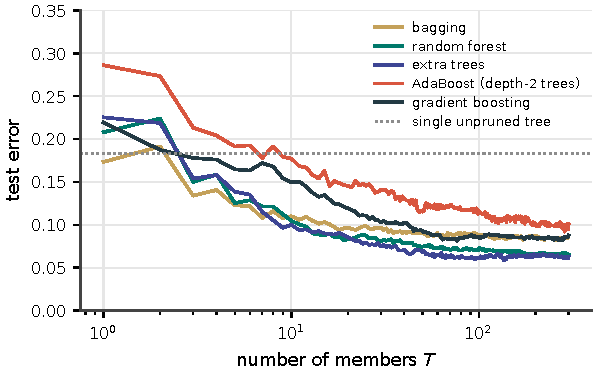
\includegraphics[width=0.76\textwidth]{ch02/ensemble_size}
\caption{Test error as a function of the number of members on a synthetic problem with 1500
training examples. The dotted line is a single unpruned tree.}
\label{fig:ensemblesize}
\end{figure}

\subsection{Decorate}

\emph{Decorate\index{Decorate|textbf}} \citep{melville2003constructing} generates diversity\index{diversity} explicitly by adding
\emph{artificial} training examples. In each iteration it generates a number of artificial
examples (a fraction of the size of the training set) from a simple model of the data
distribution, and labels them so that they \emph{differ} from the predictions of the current
ensemble. A new member is trained on the original data plus the artificial examples, and it is
kept only if it does not increase the training error of the ensemble: poor models are not
included. The probabilities of the members are averaged. The original Decorate experiments reported higher accuracy than
the base classifier and than bagging\index{bagging}, and gains over boosting in several small-sample settings, which should be
verified for the task at hand.

% ---------------------------------------------------------------------
\section{Hybrid approaches}\label{sec:hybrid}

Hybrid methods combine models learned with \emph{different} techniques. Different learning
biases produce naturally diverse models: a linear model, a nearest-neighbour\index{k-nearest neighbours@$k$-nearest neighbours} classifier and a
decision tree make different kinds of mistakes.

\subsection{Voting}

The most basic combination of heterogeneous models is voting\index{voting}: each model votes and the class
with most votes wins (\emph{hard} voting), or the probabilities are averaged (\emph{soft}
voting). Diversity\index{diversity} is generated implicitly, by the differences between the techniques. The
drawback of uniform voting is that bad models have the same importance as good ones, so voting
heterogeneous models often gives disappointing results unless all of them are reasonably good.
In \cref{lst:stacking}, hard voting of four models is barely better than the best of them
(accuracy 0.863 against 0.862), and soft voting, which uses the confidence of the members, does
a little better (0.871).

\subsection{Stacking}

\emph{Stacking\index{stacking|textbf}} (stacked generalisation\index{generalisation}, \citealp{wolpert1992stacked}) learns how to combine
the models. It uses two levels of models (\cref{fig:stacking}): the \emph{base models}
(level~0), usually learned with different techniques, and a \emph{metamodel} (level~1),
trained to optimise the fusion\index{fusion of models} of the base models' outputs. The inputs of the metamodel are the
predictions of the base models.

The key to stacking is to avoid overfitting: if the metamodel were trained on predictions that
the base models make on their own training data, it would learn to trust the models that overfit
most. The metamodel must be trained with \emph{fresh} data, that is, with predictions on
examples the base models have not seen. With enough data a separate validation set can be used;
more efficiently, the base models produce \emph{out-of-fold} predictions by cross-validation\index{cross-validation},
and are finally refitted on all the data (\cref{alg:stacking}). \citet{ting1999issues} showed
that stacking works best when the base models provide class probabilities (rather than crisp
labels) and the metamodel is a simple model such as a linear or logistic regression\index{logistic regression}. A
theoretical justification of cross-validated stacking, under the name of \emph{super learner},
was given by \citet{vanderlaan2007super}.

\begin{figure}[htbp]
\centering
\begin{tikzpicture}[font=\scriptsize\sffamily,
  box/.style={draw=edmnavy,fill=edmnavy!6,rounded corners=2pt,minimum height=6mm,align=center},
  mod/.style={draw=edmteal,fill=edmteal!10,rounded corners=2pt,minimum width=19mm,minimum height=6mm,align=center},
  meta/.style={draw=edmcoral,fill=edmcoral!10,rounded corners=2pt,minimum height=9mm,align=center},
  arr/.style={-{Stealth[length=1.8mm]},edmnavy}]
  \node[box,minimum width=14mm,minimum height=17mm] (d) at (0,0) {training\\data\\$(x_i,y_i)$};
  \node[mod] (m1) at (2.7,1.1) {neural network};
  \node[mod] (m2) at (2.7,0) {decision tree};
  \node[mod] (m3) at (2.7,-1.1) {SVM};
  \foreach \i in {1,2,3} \draw[arr] (d.east) -- (m\i.west);
  \node[box,text width=33mm,minimum height=17mm] (z) at (6.5,0)
       {meta-features (out-of-fold)\\[2pt]$z_i=\bigl(\hat p_1(x_i),\hat p_2(x_i),\hat p_3(x_i)\bigr)$};
  \foreach \i in {1,2,3} \draw[arr] (m\i.east) -- (z.west);
  \node[meta] (mm) at (10.1,0) {metamodel\\(e.g.\ logistic\\regression)};
  \draw[arr] (z) -- (mm);
  \node (pred) at (12.4,0) {prediction};
  \draw[arr] (mm) -- (pred);
  \node[text=edmteal!70!black] at (2.7,1.85) {level 0: base models};
  \node[text=edmcoral] at (10.1,0.95) {level 1};
\end{tikzpicture}
\caption{Stacking. The base models, usually learned with different techniques, produce
predictions that become the inputs of a metamodel. To avoid overfitting, the metamodel is
trained on out-of-fold (cross-validated) predictions.}
\label{fig:stacking}
\end{figure}

\begin{algorithm}[htbp]
\caption{Stacking with cross-validated meta-features}\label{alg:stacking}
\begin{algorithmic}[1]
\Require training set $D$; base learners $\mathcal A_1,\dots,\mathcal A_M$; metalearner $\mathcal B$; $K$ folds
\State split $D$ into folds $F_1,\dots,F_K$
\For{$k=1,\dots,K$}
  \For{$m=1,\dots,M$}
    \State $h_m^{(-k)}\gets\mathcal A_m(D\setminus F_k)$
    \State $z_{im}\gets h_m^{(-k)}(x_i)$ for every $x_i\in F_k$ \Comment{out-of-fold predictions}
  \EndFor
\EndFor
\State $g\gets\mathcal B\bigl(\{(z_i,y_i)\}_{i=1}^{n}\bigr)$ \Comment{train the metamodel}
\State $h_m\gets\mathcal A_m(D)$ for $m=1,\dots,M$ \Comment{refit the base models on all the data}
\State \Return $H(x)=g\bigl(h_1(x),\dots,h_M(x)\bigr)$
\end{algorithmic}
\end{algorithm}

\begin{pylisting}[label={lst:stacking}]{Base models, hard and soft voting, and stacking (5-fold CV)}
from sklearn.datasets import make_classification
from sklearn.ensemble import StackingClassifier, VotingClassifier
from sklearn.linear_model import LogisticRegression
from sklearn.model_selection import StratifiedKFold, cross_validate
from sklearn.naive_bayes import GaussianNB
from sklearn.neighbors import KNeighborsClassifier
from sklearn.pipeline import make_pipeline
from sklearn.preprocessing import StandardScaler
from sklearn.tree import DecisionTreeClassifier

X, y = make_classification(n_samples=2000, n_features=20, n_informative=6, n_redundant=4,
                           flip_y=0.05, class_sep=0.8, random_state=11)
base = [("logistic", make_pipeline(StandardScaler(), LogisticRegression())),
        ("naive Bayes", GaussianNB()),
        ("15-NN", make_pipeline(StandardScaler(), KNeighborsClassifier(15))),
        ("tree", DecisionTreeClassifier(max_depth=6, random_state=0))]
models = dict(base)
models["hard voting"] = VotingClassifier(base, voting="hard")
models["soft voting"] = VotingClassifier(base, voting="soft")
models["stacking"] = StackingClassifier(base, final_estimator=LogisticRegression(), cv=5)
cv = StratifiedKFold(5, shuffle=True, random_state=0)
for name, m in models.items():
    scoring = ["accuracy", "roc_auc"] if hasattr(m, "predict_proba") else ["accuracy"]
    r = cross_validate(m, X, y, cv=cv, scoring=scoring)
    auc = f"{r['test_roc_auc'].mean():.3f}" if "roc_auc" in scoring else "  -  "
    print(f"{name:12s} accuracy={r['test_accuracy'].mean():.3f}  AUC={auc}")
\end{pylisting}
\begin{pyoutput}
logistic     accuracy=0.840  AUC=0.907
naive Bayes  accuracy=0.845  AUC=0.908
15-NN        accuracy=0.862  AUC=0.935
tree         accuracy=0.846  AUC=0.871
hard voting  accuracy=0.863  AUC=  -  
soft voting  accuracy=0.871  AUC=0.935
stacking     accuracy=0.882  AUC=0.942
\end{pyoutput}

In \cref{lst:stacking}, stacking obtains the best accuracy (0.882) and AUC\index{area under the ROC curve (AUC)} (0.942), above every
base model and above both kinds of voting\index{voting}. Its evaluation needs the same care as any other
pipeline: the whole procedure, including the internal cross-validation, must be evaluated on
data that it has not seen (\cref{sec:protocols}).

\subsection{Cascading}

In \emph{cascade generalisation\index{cascading|textbf}\index{generalisation|textbf}} \citep{gama2000cascade} the classifiers are applied
sequentially, and each one extends the representation of the data for the next: the class
probability distribution predicted by a base classifier is added to the original attributes as
new attributes, and the next classifier learns from the extended representation. In the
original proposal this is done locally, inside the nodes of a decision tree: at each node,
base-level classifiers are induced with the examples that reach the node, and their outputs are
added as new candidate attributes for the split. A neural network, a linear regression\index{linear regression} and a
decision tree can thus be chained, each one using the previous models' outputs as additional
features.

The word \emph{cascade} is also used, in computer vision, for a different idea: a sequence of
increasingly complex classifiers in which the early, cheap ones reject the easy negative examples
and only the difficult ones reach the expensive stages. The Viola--Jones face detector
\citep{viola2001rapid} made this kind of cascade famous; its goal is speed, and it is close in
spirit to the delegating\index{delegation} classifiers of \cref{sec:cautious}.

\subsection{Mixtures of experts}

A \emph{mixture of experts\index{mixture of experts|textbf}} \citep{jacobs1991adaptive} generates several experts (classifiers or
regressors) whose outputs are combined through a (generalised) linear rule whose weights depend
on the input: a \emph{gating} model $g$ decides how much to trust each expert for each example,
\begin{equation}
  \bar f(y\mid x)=\sum_{t=1}^{T}g_t(x)\,f_t(y\mid x),\qquad
  g_t(x)=\frac{e^{v_t^{\top}x}}{\sum_{s}e^{v_s^{\top}x}}.
\end{equation}
Experts and gate are trained together, classically with the expectation--maximisation\index{expectation maximisation (EM)} (EM)
algorithm, and both use the input examples, so each expert specialises in a region of the input
space. Several mixtures can be combined in a tree, giving a \emph{hierarchical} mixture of
experts \citep{jordan1994hierarchical}. Mixtures of experts are useful when the experts are
diverse, and the idea has had a spectacular revival in deep learning: \emph{sparse} mixtures of
experts, in which the gate activates only a few experts for each input, allow enormous neural
networks, including several large language models\index{large language model (LLM)}\index{language model}, to be trained and run at a fraction of the
cost of a dense network of the same size \citep{shazeer2017outrageously,fedus2022switch}.

% ---------------------------------------------------------------------
\section{Knowing when not to predict: abstention and delegation}\label{sec:cautious}

Combining models is one way of dealing with their limitations. Another is to let a model admit
them. Deployed systems rarely face only the choice ``predict class $a$ or class $b$'': there is
almost always a third option, \emph{do not decide here and pass the case on}. A fraud detector
sends doubtful transactions to a team of analysts; a triage system refers unclear cases to a
doctor; a content moderation pipeline escalates borderline posts to human reviewers; a cheap
model answers the easy queries and calls an expensive one for the hard ones. This section
studies the two forms of the idea: \emph{abstaining}, where a cautious classifier\index{cautious classifier} says ``I do not
know'' and someone else (often a person) decides, and \emph{delegating\index{delegation|textbf}}, where the classifier
passes the case to another model.

\subsection{The reject option}

Let us add to the possible decisions an extra one, ``unknown'', denoted $\perp$, which has a cost
$c_r$. As in \cref{sec:costs}, the best decision for an example is the one with the lowest
expected cost\index{expected cost}, now with one more option: \emph{abstain\index{abstention|textbf} when every prediction has a higher
expected cost than abstaining}.

\citet{chow1970optimum} derived the optimal rule for the simplest case: errors cost 1, correct
predictions cost 0, and abstaining costs $c_r$ (with $0\leq c_r\leq1/2$). The expected cost of
predicting the most probable class is $1-\max_ip_i$, so, with calibrated probabilities, it is
optimal to abstain whenever
\begin{equation}\label{eq:chow}
  \max_i\,p_i<1-c_r .
\end{equation}
The cheaper abstaining is, the more often the classifier should abstain.

With unequal error costs the reasoning is the same. For two classes, if $p$ is the probability
of the positive class, predicting positive costs $(1-p)\,c_{\mathrm{FP}}$ on average, predicting
negative costs $p\,c_{\mathrm{FN}}$, and abstaining costs $c_r$. Abstaining is optimal when both
predictions are more expensive than abstaining, that is, when
\begin{equation}\label{eq:rejectband}
  \frac{c_r}{c_{\mathrm{FN}}}<p<1-\frac{c_r}{c_{\mathrm{FP}}}.
\end{equation}
The classifier abstains on a band of probabilities that contains the cost threshold
$t^\star=c_{\mathrm{FP}}/(c_{\mathrm{FP}}+c_{\mathrm{FN}})$ of \cref{eq:tstar}; the band is empty, and
abstaining is never worthwhile, when
$c_r\geq c_{\mathrm{FP}}c_{\mathrm{FN}}/(c_{\mathrm{FP}}+c_{\mathrm{FN}})$. With more classes, the cost
matrix\index{cost matrix} simply gets an extra row for $\perp$.

\begin{example}{When abstaining is the best decision}{costcautious}
A three-class problem has the following costs (rows: decision; columns: actual class; negative
values are benefits). Abstaining costs nothing.
\begin{center}\small
\begin{tabular}{@{}lrrr@{}}
\toprule
{\footnotesize decision\,\textbackslash\,actual} & $a$ & $b$ & $c$\\
\midrule
$a$ & $-2.5$ & $4$ & $2$\\
$b$ & $2.1$ & $-3.5$ & $0$\\
$c$ & $1.2$ & $1.3$ & $-4$\\
$\perp$ & $0$ & $0$ & $0$\\
\bottomrule
\end{tabular}
\end{center}
For an example with probabilities $(0.40,0.35,0.25)$ the expected costs of predicting $a$, $b$,
$c$ and $\perp$ are $0.9$, $-0.385$, $-0.065$ and $0$: the best decision is $b$, although $a$ is
more probable. For $(0.50,0.28,0.22)$ they are $0.31$, $0.07$, $0.084$ and $0$: every prediction
has a positive expected cost, and the best decision is to abstain, although $a$ has a
probability of 0.5 (part (a) of \cref{lst:costcautious}).
\end{example}

\subsection{Evaluating cautious classifiers}

A \emph{cautious classifier\index{cautious classifier|textbf}} \citep{ferri2004cautious} adds the class $\perp$ to the set of
original classes $C$. It must find a compromise between reducing the number of misclassified
examples (\emph{error}) and reducing the number of unclassified examples (\emph{abstention\index{abstention|textbf}}):
abstaining always is never wrong and never useful. Its confusion matrix\index{confusion matrix} has an extra row for
$\perp$. If $M(i,j)$ counts the examples predicted as $i\in C\cup\{\perp\}$ whose actual class is
$j\in C$, and $\mathit{Card}$ is the total number of examples:
\begin{align}
  \text{Coverage}&=\frac{\sum_{i\in C,\,j\in C}M(i,j)}{\mathit{Card}}, &
  \text{Abstention}&=\frac{\sum_{j\in C}M(\perp,j)}{\mathit{Card}},\\
  \text{Accuracy}&=\frac{\sum_{i\in C}M(i,i)}{\sum_{i\in C,\,j\in C}M(i,j)}, &
  \text{Error}&=\frac{\sum_{i,j\in C,\,i\neq j}M(i,j)}{\mathit{Card}}.
\end{align}
The accuracy is computed on the \emph{covered} examples, whereas the error is relative to all of
them. They satisfy $\text{Coverage}+\text{Abstention}=1$ and
$\text{Accuracy}\times\text{Coverage}=\text{Coverage}-\text{Error}$.

\begin{example}{Evaluating a cautious classifier}{cautious}
A cautious classifier with classes $\{a,b,c\}$ produces this confusion matrix on 100 test
examples (rows: predicted; columns: actual):
\begin{center}\small
\begin{tabular}{@{}lccc@{}}
\toprule
{\footnotesize pred.\,\textbackslash\,actual} & $a$ & $b$ & $c$\\
\midrule
$a$ & 19 & 1 & 2\\
$b$ & 0 & 30 & 0\\
$c$ & 0 & 1 & 38\\
$\perp$ & 1 & 2 & 6\\
\bottomrule
\end{tabular}
\end{center}
It classifies 91 examples and abstains on 9: coverage\index{coverage} 0.91 and abstention 0.09. Of the 91
classified examples, 87 are correct: accuracy $87/91=0.956$. The four mistakes give an error of
$4/100=0.04$, and indeed $0.956\times0.91=0.87=0.91-0.04$ (\cref{lst:cautious}).
\end{example}

A single matrix describes one operating point\index{operating point}. The quality of a cautious classifier is the whole
trade-off, which is shown in an \emph{accuracy\index{accuracy|textbf} response graph}: the accuracy on the covered
examples against the abstention, obtained by abstaining on increasingly large fractions of the
least confident examples (\cref{fig:cautious}a). The literature on \emph{selective
classification} shows the same information as a \emph{risk--coverage\index{risk--coverage curve|textbf}} curve, the error on the
covered examples against the coverage \citep{elyaniv2010foundations,geifman2017selective}. Two
summaries are useful: the accuracy at the level of abstention that the application can afford
(say, 20\%), and the \emph{area under the risk--coverage curve} (AURC\index{AURC}), the average error of the
$k$ most confident predictions over all values of $k$ \citep{geifman2019bias}; lower is better.

What makes a good cautious classifier is not its accuracy but whether its confidence
\emph{ranks its own mistakes}: the examples it is least sure about must be the ones it would get
wrong. This can be measured directly as the AUC of the confidence for separating correct from
incorrect predictions (\cref{sec:roc}), and it depends on the quality of the probabilities
(\cref{sec:calibration}). In \cref{fig:cautious}a, the decision tree is the most accurate
classifier when it must classify everything (0.824), but its confidence, based on a few leaf
frequencies, ranks its errors poorly (AUC 0.648, against 0.700 for logistic regression and 0.724
for naive Bayes\index{naive Bayes}): its curve flattens and then falls, and it has the worst AURC (0.147). Naive
Bayes has the best AURC (0.101) and becomes the most accurate model above 50\% abstention. The tree
produces only a few distinct confidences, so the order of the examples within ties changes its curve
and its AURC: a tie policy must be stated, for instance averaging over random orders. Which
model is best depends on how much abstention the application can tolerate.

Naive Bayes deserves a second look, because \cref{sec:calibration} showed that its probabilities are badly
calibrated. There is no contradiction: abstaining on a fixed share of the least confident cases, as AURC and
delegation\index{delegation} do, only needs a confidence that \emph{ranks} the errors well (any strictly increasing transformation of
it gives the same curve), whereas abstaining with cost-based thresholds, as the window rule\index{window rule} below does, needs
probabilities that are \emph{calibrated\index{calibration|textbf}}. Part~(c) of \cref{lst:costcautious} applies the cost-matched window rule
to naive Bayes on the same data: uncalibrated, it abstains on 22.8\% of the test cases at a mean cost of 0.326;
after isotonic\index{calibration!isotonic regression} calibration it abstains on 36.3\% at a mean cost of 0.312.

\begin{pylisting}[label={lst:cautious}]{Evaluation of a cautious classifier, and how well three models rank their own errors}
import numpy as np
from sklearn.datasets import make_classification
from sklearn.linear_model import LogisticRegression
from sklearn.metrics import roc_auc_score
from sklearn.model_selection import train_test_split
from sklearn.naive_bayes import GaussianNB
from sklearn.tree import DecisionTreeClassifier

# (a) Rows = predicted a, b, c and "unknown"; columns = actual a, b, c
M = np.array([[19, 1, 2], [0, 30, 0], [0, 1, 38], [1, 2, 6]])
card, covered, hits = M.sum(), M[:3].sum(), np.trace(M[:3])
print(f"coverage={covered / card:.2f}  abstention={M[3].sum() / card:.2f}  "
      f"accuracy={hits / covered:.3f}  error={(covered - hits) / card:.2f}")

# (b) Does the confidence of each model rank its own mistakes?
X, y = make_classification(n_samples=4000, n_features=20, n_informative=6, n_redundant=4,
                           flip_y=0.05, class_sep=0.8, random_state=5)
X_tr, X_te, y_tr, y_te = train_test_split(X, y, test_size=0.5, random_state=0)
for name, m in [("logistic", LogisticRegression(max_iter=1000)),
                ("naive Bayes", GaussianNB()),
                ("tree (depth 6)", DecisionTreeClassifier(max_depth=6, random_state=0))]:
    P = m.fit(X_tr, y_tr).predict_proba(X_te)
    conf, correct = P.max(axis=1), P.argmax(axis=1) == y_te
    ok = correct[np.argsort(-conf, kind="stable")]            # most confident first
    risk = 1 - np.cumsum(ok) / np.arange(1, len(ok) + 1)      # error of the top-k
    acc20 = 1 - risk[int(0.8 * len(ok)) - 1]                  # with 20% abstention
    auc = roc_auc_score(correct, conf)                        # confidence vs correctness
    print(f"{name:14s} acc={correct.mean():.3f}  acc@20%abst={acc20:.3f}  "
          f"AURC={risk.mean():.3f}  AUC(conf)={auc:.3f}")
\end{pylisting}
\begin{pyoutput}
coverage=0.91  abstention=0.09  accuracy=0.956  error=0.04
logistic       acc=0.766  acc@20%abst=0.814  AURC=0.129  AUC(conf)=0.700
naive Bayes    acc=0.792  acc@20%abst=0.843  AURC=0.101  AUC(conf)=0.724
tree (depth 6) acc=0.824  acc@20%abst=0.874  AURC=0.147  AUC(conf)=0.648
\end{pyoutput}

\subsection{From probabilistic to cautious classifiers}

Any probabilistic classifier $f$, which assigns to each example a vector of $|C|$ probabilities
$p_i$, can be turned into a cautious classifier\index{cautious classifier}. Following \citet{ferri2004cautious}, define a
\emph{class bias} $K=\{k_i\}_{i=1}^{|C|}$ with $\sum_ik_i=1$, and a \emph{window size}
$w\in[0,1]$:
\begin{center}
\fbox{\begin{minipage}{0.86\textwidth}
\textbf{Decision rule\index{decision rules|textbf}} (given $K$ and $w$). For each class $i$, compute the threshold
$\tau_i=(1-k_i)\,w+k_i$. If some $p_i\geq\tau_i$, predict $\argmax_i\,(p_i/\tau_i)$ among those
classes; otherwise predict $\perp$.
\end{minipage}}
\end{center}
With $w=0$ the thresholds are the class biases themselves and the classifier never abstains\index{abstention}: with
a uniform $K$ it predicts the most probable class, and with a non-uniform $K$ it shifts the
decision towards some classes, as a cost-sensitive\index{cost-sensitive learning} threshold does. As $w$ grows, the thresholds
move towards 1 and the classifier abstains more and more; with $w=1$ it only predicts when it is
completely sure.

For two classes the rule has a simple geometry. If $k$ is the bias of the positive class, it
predicts positive when $p\geq k+(1-k)\,w$, negative when $p\leq k\,(1-w)$, and abstains in
between,
\begin{equation}\label{eq:windowband}
  k\,(1-w)<p<k+(1-k)\,w,
\end{equation}
a \emph{window} around $k$ whose width grows with $w$. Comparing it with the optimal band of
\cref{eq:rejectband} gives a remarkable result. Take $k=t^\star$ and
\begin{equation}\label{eq:wstar}
  w^\star=1-\frac{c_r\,(c_{\mathrm{FP}}+c_{\mathrm{FN}})}{c_{\mathrm{FP}}\,c_{\mathrm{FN}}}.
\end{equation}
Then $k(1-w^\star)=\frac{c_{\mathrm{FP}}}{c_{\mathrm{FP}}+c_{\mathrm{FN}}}\cdot
\frac{c_r(c_{\mathrm{FP}}+c_{\mathrm{FN}})}{c_{\mathrm{FP}}c_{\mathrm{FN}}}=\frac{c_r}{c_{\mathrm{FN}}}$
and, in the same way, $k+(1-k)\,w^\star=1-(1-k)(1-w^\star)=1-\frac{c_r}{c_{\mathrm{FP}}}$: the two
bands coincide.

\begin{keyidea}
For two classes, the window rule\index{window rule} with the class bias matched to the error costs,
$K=(1-t^\star,t^\star)$, and the window $\max(0,w^\star)$, with $w^\star$ from \cref{eq:wstar}, \emph{is} the
optimal cost-sensitive reject rule for positive error costs, given the probabilities it receives; when
$c_r\geq c_{\mathrm{FP}}c_{\mathrm{FN}}/(c_{\mathrm{FP}}+c_{\mathrm{FN}})$ the window is 0 and abstaining never pays. Chow's rule is the special case of equal costs: $K=(0.5,0.5)$ and
$w^\star=1-2c_r$. The class bias $K$ encodes the costs of the errors; the window $w$ encodes the
cost of abstaining.
\end{keyidea}

For instance, with $c_{\mathrm{FP}}=1$, $c_{\mathrm{FN}}=4$ and $c_r=0.5$, the cost threshold is
$t^\star=0.2$, the window is $w^\star=1-0.5\cdot5/4=0.375$, and both rules abstain exactly when
$0.125<p<0.5$; part (b) of \cref{lst:costcautious} checks that they take the same decision for
every probability. \Cref{fig:cautious}b shows what is at stake on a problem with 20\% of positives.
With a uniform $K$ and $w=0$ the logistic regression uses the threshold 0.5, ignores the costs,
and costs 0.537 per example; with the cost-matched $K$ it costs 0.386 without abstaining at all.
As $w$ grows both curves fall, because abstaining (0.5) is cheaper than many risky predictions;
the cost-matched curve stays below the uniform one, and its minimum is reached at $w^\star$ (the
star: 42\% of abstentions and a cost of 0.327 per example), where it makes exactly the decisions
of the optimal rule. With more than two classes the window rule is not always identical to the
optimal one, but $K$ and $w$ keep the same interpretation.

\begin{figure}[htbp]
\centering
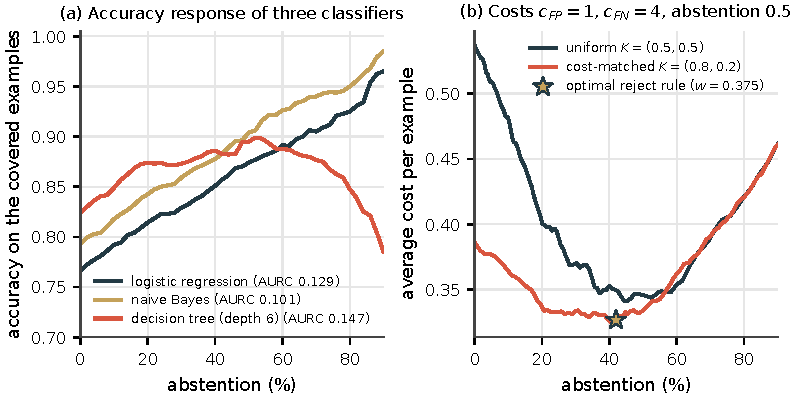
\includegraphics[width=\textwidth]{ch02/cautious}
\caption{(a) Accuracy response graphs of three classifiers (2000 test examples); the AURC
summarises each curve. (b) Average cost of a logistic regression turned into a cautious
classifier with the window rule, for a uniform and a cost-matched class bias, as the window
grows; the star is the optimal reject rule.}
\label{fig:cautious}
\end{figure}

\begin{pylisting}[label={lst:costcautious}]{Expected costs with an abstention option, and the window rule as the optimal reject rule}
import numpy as np
from sklearn.calibration import CalibratedClassifierCV
from sklearn.datasets import make_classification
from sklearn.model_selection import train_test_split
from sklearn.naive_bayes import GaussianNB

# (a) Costs: rows = decision (a, b, c, unknown), columns = actual class (a, b, c)
C = np.array([[-2.5,  4.0,  2.0],
              [ 2.1, -3.5,  0.0],
              [ 1.2,  1.3, -4.0],
              [ 0.0,  0.0,  0.0]])
decisions = np.array(["a", "b", "c", "unknown"])
for p in ([0.40, 0.35, 0.25], [0.50, 0.28, 0.22]):
    ec = C @ np.array(p)                       # expected cost of each decision
    print(f"p={p}  expected costs={ec.round(3)}  ->  {decisions[ec.argmin()]}")

# (b) Two classes: the window rule with a cost-matched K is the optimal reject rule
def cautious_predict(P, K, w):
    tau = (1 - np.asarray(K)) * w + np.asarray(K)      # one threshold per class
    ok = P >= tau
    pred = np.where(ok, P / tau, -np.inf).argmax(axis=1)
    pred[~ok.any(axis=1)] = -1                          # -1 means "unknown"
    return pred

c_fp, c_fn, c_r = 1.0, 4.0, 0.5
t = c_fp / (c_fp + c_fn)                                # cost threshold t*
w = 1 - c_r * (c_fp + c_fn) / (c_fp * c_fn)
p = np.linspace(0.0005, 0.9995, 1000)                   # P(positive)
window = cautious_predict(np.c_[1 - p, p], K=(1 - t, t), w=w)
cost = np.c_[p * c_fn, (1 - p) * c_fp, np.full_like(p, c_r)]   # predict 0, 1, abstain
bayes = np.array([0, 1, -1])[cost.argmin(axis=1)]
print(f"t*={t:.2f}  w={w:.3f}  identical decisions: {np.mean(window == bayes):.3f}")
print(f"abstains for p in [{p[window == -1].min():.4f}, {p[window == -1].max():.4f}]")

# (c) Data of Listing 2.9: ranking errors well is not enough, the window needs calibration
X, y = make_classification(n_samples=4000, n_features=20, n_informative=6, n_redundant=4,
                           flip_y=0.05, class_sep=0.8, random_state=5)
X_tr, X_te, y_tr, y_te = train_test_split(X, y, test_size=0.5, random_state=0)
for name, m in [("naive Bayes", GaussianNB()),
                ("naive Bayes + isotonic",
                 CalibratedClassifierCV(GaussianNB(), method="isotonic"))]:
    p1 = m.fit(X_tr, y_tr).predict_proba(X_te)[:, 1]
    d = cautious_predict(np.c_[1 - p1, p1], K=(1 - t, t), w=w)
    loss = np.where(d == -1, c_r, np.where(d == 1, (y_te == 0) * c_fp, (y_te == 1) * c_fn))
    print(f"{name:23s} abstains {np.mean(d == -1):.3f}  mean cost {loss.mean():.3f}")
\end{pylisting}
\begin{pyoutput}
p=[0.4, 0.35, 0.25]  expected costs=[ 0.9   -0.385 -0.065  0.   ]  ->  b
p=[0.5, 0.28, 0.22]  expected costs=[0.31  0.07  0.084 0.   ]  ->  unknown
t*=0.20  w=0.375  identical decisions: 1.000
abstains for p in [0.1255, 0.4995]
naive Bayes             abstains 0.228  mean cost 0.326
naive Bayes + isotonic  abstains 0.363  mean cost 0.312
\end{pyoutput}

Conformal prediction\index{conformal prediction} (\cref{sec:other}) offers another way of deciding when to abstain, with a
different guarantee: compute prediction sets with coverage\index{coverage} $1-\alpha$ and abstain whenever the
set does not contain exactly one label: two or more labels signal ambiguity\index{ambiguity decomposition}, and an empty set signals that
no label is plausible, as for an input unlike the calibration data. In \cref{lst:conformalabst}, 90\% prediction sets cover 90.1\%
of the test examples; 67.0\% of them contain a single label, with an accuracy of 0.853; the other
33.0\% contain both labels, and no set is empty with this $\alpha$, although empty sets become possible as $\alpha$
grows. The guarantee concerns the coverage of the sets,
not the accuracy of the single-label predictions.

\begin{pylisting}[label={lst:conformalabst}]{Abstaining when a conformal prediction set is not a single label}
import numpy as np
from sklearn.datasets import make_classification
from sklearn.linear_model import LogisticRegression
from sklearn.model_selection import train_test_split

X, y = make_classification(n_samples=6000, n_features=20, n_informative=6, n_redundant=4,
                           flip_y=0.05, class_sep=0.8, random_state=5)
X_tr, X_rest, y_tr, y_rest = train_test_split(X, y, test_size=2 / 3, random_state=0)
X_cal, X_te, y_cal, y_te = train_test_split(X_rest, y_rest, test_size=0.5, random_state=1)
model = LogisticRegression(max_iter=1000).fit(X_tr, y_tr)

alpha = 0.1                                                  # 90% prediction sets
s_cal = 1 - model.predict_proba(X_cal)[np.arange(len(y_cal)), y_cal]
k = int(np.ceil((len(y_cal) + 1) * (1 - alpha)))      # rank of the conformal quantile
q = np.inf if k > len(y_cal) else np.sort(s_cal)[k - 1]
sets = 1 - model.predict_proba(X_te) <= q                    # label j in the set?
size = sets.sum(axis=1)
one = size == 1                                              # predict; otherwise abstain
covered = np.mean(sets[np.arange(len(y_te)), y_te])
print(f"set coverage={covered:.3f} (target {1 - alpha:.2f})")
print(f"single-label sets={one.mean():.3f}  abstain: two labels={np.mean(size == 2):.3f}  "
      f"empty={np.mean(size == 0):.3f}")
acc_one = np.mean(sets[one].argmax(axis=1) == y_te[one])
print(f"accuracy on single-label sets={acc_one:.3f}")
\end{pylisting}
\begin{pyoutput}
set coverage=0.901 (target 0.90)
single-label sets=0.670  abstain: two labels=0.330  empty=0.000
accuracy on single-label sets=0.853
\end{pyoutput}

\subsection{Delegating classifiers}

Abstaining is not always an option: a bank must eventually accept or reject the loan. A
\emph{delegating\index{delegation|textbf} classifier} \citep{ferri2004delegating} delegates the difficult or uncertain
predictions to other, possibly more specialised, classifiers. In the \emph{two-step scenario}, a
first classifier is learned from all the training data; it keeps the examples on which it is
confident and delegates the rest, and a second classifier is learned from the delegated training
examples only. At prediction time, each new example is classified by the first classifier if its
confidence exceeds the threshold, and passed to the second one otherwise. In the \emph{iterated
scenario}, an arbitrary number of classifiers are chained in the same way. In the \emph{round
rebound\index{round rebound|textbf}} variant (\cref{fig:delegation}), the cases that are very difficult for the second level,
those on which it is not confident either, come back to the first level, which makes the final
prediction.

\begin{figure}[htbp]
\centering
\begin{tikzpicture}[font=\scriptsize\sffamily,
  box/.style={draw=edmnavy,fill=edmnavy!6,rounded corners=2pt,minimum height=7mm,align=center},
  mod/.style={draw=edmteal,fill=edmteal!10,rounded corners=2pt,minimum width=17mm,minimum height=7mm,align=center},
  dec/.style={diamond,draw=edmcoral,fill=edmcoral!8,aspect=2.3,inner sep=1pt,align=center},
  arr/.style={-{Stealth[length=1.8mm]},edmnavy}]
  \node[box] (x) at (0,0) {new\\example $x$};
  \node[mod] (c1) at (2.2,0) {classifier 1};
  \node[dec] (q1) at (4.6,0) {confident?\\$c_1(x)>\theta_1$};
  \node[box,minimum width=36mm] (p1) at (8.6,1.25) {prediction of classifier 1};
  \node[mod] (c2) at (7.4,-1.25) {classifier 2};
  \node[dec] (q2) at (9.9,-1.25) {confident?\\$c_2(x)>\theta_2$};
  \node[box] (p2) at (12.7,-1.25) {prediction of\\classifier 2};
  \draw[arr] (x) -- (c1);
  \draw[arr] (c1) -- (q1);
  \draw[arr] (q1.north) |- node[above,pos=0.75] {yes} (p1.west);
  \draw[arr] (q1.south) |- node[below,pos=0.75] {no: delegate} (c2.west);
  \draw[arr] (c2) -- (q2);
  \draw[arr] (q2) -- node[above] {yes} (p2);
  \draw[arr,dashed,edmcoral] (q2.north) -- node[right,pos=0.45,text=edmcoral,align=left]
       {no: round\\rebound} (q2.north |- p1.south);
\end{tikzpicture}
\caption{Two-step delegation with round rebound. The second classifier is trained on the
examples that the first one delegates, so it specialises in the difficult cases; the cases on
which it is not confident either go back to the first level (dashed arrow).}
\label{fig:delegation}
\end{figure}

Delegation serves two different purposes, depending on the second level:
\begin{itemize}
  \item \emph{specialisation}: as in the original proposal, the second classifier is learned
        from the delegated examples and becomes an expert in the difficult region. Each
        classifier learns from fewer examples than the previous one, which makes delegation
        \emph{efficient}; every prediction is made by a single classifier, which keeps the system
        \emph{comprehensible\index{comprehensibility|textbf}} (with decision trees, it is a short list of trees with confidence
        conditions); and the parts of the system that lead to delegation can be removed to
        simplify it;
  \item \emph{efficiency} (a \emph{cascade\index{cascading|textbf}}): the second level is a stronger but more expensive
        model, trained on all the data, and the first level answers the easy cases cheaply. The
        aim is to obtain most of the accuracy of the expensive model while calling it for only a
        fraction of the examples.
\end{itemize}

\Cref{fig:graphdelegation} and \cref{lst:delegation} compare the variants, with a decision tree of
16 leaves as first level. The delegation thresholds are taken from \emph{out-of-fold} confidences
(\cref{sec:protocols}): on its own training data a model is overconfident, so a quantile of those confidences would
delegate fewer new examples than intended. Delegating to a random forest raises the accuracy from 0.803 (the tree
alone) to 0.882, closing three quarters of the gap with the forest (0.908) while calling it for only 717 of the 3000
test examples (24\%, not the nominal 30\%: the tree produces only 16 distinct confidences, so the quantile is
coarse), and every prediction that is not delegated can be explained by the small tree. A specialist tree trained on
the delegated examples reaches 0.842 (and 0.850 at best); its curve is irregular because each delegation threshold
produces a different training set for the specialist. Round rebound returns 227 of the 717 delegated cases to the
first tree and leaves the accuracy unchanged here (0.842): the cases that bounce back are, by construction, those the
first tree had already found difficult, so it is no better than the specialist on them. Rebound pays off only when
the first level remains competent on part of the region it delegates. As with every design choice in this book, the
variant must be validated on data (Exercise~\ref{exr2:rebound}). The delegation rate is measured on the test data,
because no quantile estimated during training guarantees the same rate in deployment\index{deployment}, and the time actually saved
must be measured as well, since the cost of the second level depends on the hardware and on batching.

\begin{figure}[htbp]
\centering
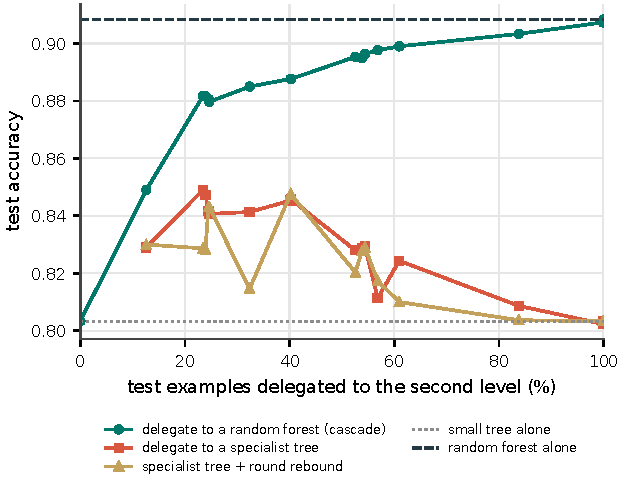
\includegraphics[width=0.78\textwidth]{ch02/delegation}
\caption{Accuracy of three delegation schemes as a function of the fraction of test examples sent
to the second level. The first level is a decision tree with 16 leaves; the cascade delegates to
a random forest of 200 trees trained on all the data.}
\label{fig:graphdelegation}
\end{figure}

\begin{pylisting}[label={lst:delegation}]{Two-step delegation: specialist, round rebound and cascade}
import numpy as np
from sklearn.datasets import make_classification
from sklearn.ensemble import RandomForestClassifier
from sklearn.model_selection import cross_val_predict, train_test_split
from sklearn.tree import DecisionTreeClassifier

class DelegatingClassifier:
    """Two-step delegation (after Ferri, Flach and Hernandez-Orallo, 2004).
    The first model delegates its least confident fraction of the examples. If
    specialise=True the second model is trained only on the delegated examples; if
    rebound > 0, it returns its own least confident fraction to the first model."""
    def __init__(self, first, second, delegate=0.3, specialise=True, rebound=0.0):
        self.first, self.second, self.delegate = first, second, delegate
        self.specialise, self.rebound = specialise, rebound

    def fit(self, X, y):
        # thresholds from out-of-fold confidences: on its own training data a model
        # is overconfident, so training quantiles would delegate too few new examples
        oof = lambda m, A, b: cross_val_predict(m, A, b, cv=5, method="predict_proba")
        conf = oof(self.first, X, y).max(axis=1)
        self.first.fit(X, y)
        self.t1_ = np.quantile(conf, self.delegate)
        hard = conf <= self.t1_                               # delegated examples
        Xs, ys = (X[hard], y[hard]) if self.specialise else (X, y)
        self.second.fit(Xs, ys)
        if self.rebound:
            conf2 = oof(self.second, Xs, ys).max(axis=1)
            self.t2_ = np.quantile(conf2 if self.specialise else conf2[hard], self.rebound)
        else:
            self.t2_ = -np.inf
        return self

    def predict(self, X):
        """The first model sees every example, the second only the delegated ones."""
        P1 = self.first.predict_proba(X)
        pred = self.first.classes_[P1.argmax(axis=1)]
        idx = np.flatnonzero(P1.max(axis=1) <= self.t1_)          # delegated examples
        self.n_second_ = len(idx)
        if len(idx):
            P2 = self.second.predict_proba(X[idx])
            take = P2.max(axis=1) > self.t2_                       # else: round rebound
            pred[idx[take]] = self.second.classes_[P2[take].argmax(axis=1)]
        return pred

X, y = make_classification(n_samples=6000, n_features=10, n_informative=6, n_redundant=2,
                           flip_y=0.03, class_sep=1.0, random_state=8)
X_tr, X_te, y_tr, y_te = train_test_split(X, y, test_size=0.5, random_state=0)
tree = lambda: DecisionTreeClassifier(max_depth=4, random_state=0)
forest = lambda: RandomForestClassifier(200, random_state=0)
systems = {"small tree alone": tree(),
           "specialist (two small trees)": DelegatingClassifier(tree(), tree()),
           "specialist + round rebound": DelegatingClassifier(tree(), tree(), rebound=0.3),
           "cascade: small tree -> forest":
               DelegatingClassifier(tree(), forest(), specialise=False),
           "random forest alone": forest()}
for name, m in systems.items():
    acc = np.mean(m.fit(X_tr, y_tr).predict(X_te) == y_te)
    calls = ""
    if hasattr(m, "n_second_"):                       # delegating systems
        calls = f"  (second model: {m.n_second_} of {len(y_te)})"
    print(f"{name:30s} accuracy={acc:.3f}{calls}")
\end{pylisting}
\begin{pyoutput}
small tree alone               accuracy=0.803
specialist (two small trees)   accuracy=0.842  (second model: 717 of 3000)
specialist + round rebound     accuracy=0.842  (second model: 717 of 3000)
cascade: small tree -> forest  accuracy=0.882  (second model: 717 of 3000)
random forest alone            accuracy=0.908
\end{pyoutput}

\subsection{Delegating to humans and to large models}

When the second level is a person, delegation\index{delegation} becomes \emph{learning to defer}
\citep{madras2018predict,mozannar2020consistent}. The decision to defer should depend not only
on the confidence of the model but also on how good the human is on each kind of case: a model
should defer the cases that the human is likely to get right and it is likely to get wrong, so
the classifier and the deferral rule are trained together to minimise the error of the
human--machine team rather than that of the model alone. Deferring well can also make the whole
system fairer, if the model is less reliable for some groups of people
\citep{madras2018predict}. The same structure appears with large language models\index{large language model (LLM)}: a model
\emph{cascade\index{cascading|textbf}} sends each query to a cheap model first and uses a scoring function to decide
whether to accept its answer or escalate to a more expensive model, which can match the accuracy
of the most expensive model at a much lower cost \citep{chen2023frugalgpt}. The gating network of
a mixture of experts\index{mixture of experts} (\cref{sec:hybrid}) is yet another form of routing.

Evaluating these systems requires the quantities of this section: the accuracy or the cost as a
function of the fraction of delegated cases, and the workload sent to the human team or to the
expensive model. Once the system is deployed, the delegation rate itself is worth monitoring\index{monitoring}
(Unit~6): if a model starts to abstain\index{abstention} or delegate much more often than during validation, the
data have probably changed.

% ---------------------------------------------------------------------
\section{How good are combinations in practice?}\label{sec:performance}

\subsection{Bagging, boosting, randomisation and noise}

\citet{dietterich2000experimental} compared experimentally three methods for constructing
ensembles of decision trees: boosting, bagging\index{bagging} and randomisation\index{randomisation}. In problems without noise,
boosting obtained the best results, and bagging and randomisation were quite similar. In noisy
data sets, however, bagging was the best method, followed by randomisation, and boosting was
the worst. \citet{bauer1999empirical} obtained similar results in a large comparison of voting\index{voting}
methods.

\Cref{fig:noise} reproduces the experiment on synthetic data, flipping\index{attribute flipping} a fraction of the training
labels while testing on clean data. Without noise, AdaBoost\index{AdaBoost} is the most accurate method (0.898,
against 0.893 for the random forest and 0.885 for bagging). With 10\% of noise it has already
fallen behind both (0.848, against 0.888 and 0.870), and with 30\% the gap is large (0.686,
against 0.786 and 0.772). The reason is the exponential loss discussed in \cref{sec:ensembles}:
mislabelled\index{label noise} examples are, by definition, those the ensemble keeps getting wrong, and AdaBoost
keeps increasing their weight until the new members are devoted to fitting the noise.

\begin{figure}[htbp]
\centering
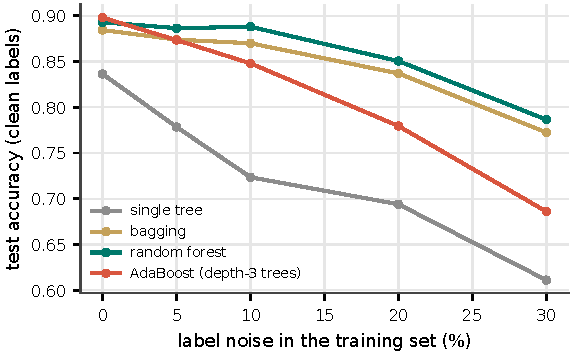
\includegraphics[width=0.72\textwidth]{ch02/noise}
\caption{Test accuracy as a function of the proportion of mislabelled training examples
(average over four synthetic data sets; test labels are clean).}
\label{fig:noise}
\end{figure}

\subsection{Large-scale comparisons}

Several large studies have compared learning algorithms across many problems:
\begin{itemize}
  \item \citet{caruana2004data} compared SVMs, neural networks, decision trees, $k$-NN, bagged
        trees, boosted trees and boosted stumps\index{decision stump} on seven problems with nine metrics, including
        threshold metrics (accuracy, $F$-score, lift\index{lift}), ranking metrics (ROC area, average
        precision\index{average precision}\index{precision}, break-even point) and probability metrics (squared error, cross-entropy\index{log loss},
        calibration). Boosted trees were excellent on the threshold and ranking metrics but
        poorly calibrated; once calibrated with Platt\index{calibration!Platt scaling}'s method (\cref{sec:calibration}) they
        became the best method. Bagged trees performed well and are very easy to train.
  \item \citet{caruana2006empirical} extended the comparison to ten methods and eleven problems:
        calibrated boosted trees were the best method overall, followed closely by random
        forests and then by bagged trees, calibrated SVMs and neural networks.
  \item \citet{fernandezdelgado2014we} evaluated 179 classifiers from 17 families on 121 data
        sets. The best classifier was a random forest, which reached on average 94.1\% of the
        maximum accuracy obtained on each data set, followed by an SVM with Gaussian kernel
        (92.3\%). A few models were clearly better than the rest (random forests, Gaussian SVMs,
        extreme learning machines with Gaussian kernel, C5.0 and averaged neural networks), and
        the random forest family was the best, followed by SVMs, neural networks and boosting
        ensembles. A later re-analysis pointed out problems in the experimental protocol and found that,
        once they were corrected, the differences between the top methods were not
        statistically significant\index{statistical significance} \citep{wainberg2016random}, a good reminder of the lessons of
        Unit~1.
  \item In data science competitions, analyses of the winning solutions show that gradient
        boosting\index{gradient boosting} libraries dominate problems with tabular data, while deep neural networks
        dominate images, audio and text. Recent benchmarks confirm that tree-based ensembles still
        outperform deep learning on typical medium-sized tabular data
        \citep{grinsztajn2022why,shwartzziv2022tabular}.
\end{itemize}

\subsection{A small benchmark}

To close the section, \cref{fig:cdens} compares seven methods on the twelve synthetic data sets
used in \cref{sec:stats}, with the AUC estimated by 5-fold cross-validation and the Friedman and
Nemenyi\index{Nemenyi test} tests. Every ensemble improves dramatically on a single tree (mean AUC 0.856): bagging\index{bagging}
0.922, random forests 0.923, extremely randomised trees\index{extra trees} 0.928, AdaBoost\index{AdaBoost} 0.911, histogram gradient
boosting\index{gradient boosting} 0.923 and stacking\index{stacking} 0.921. The Friedman test\index{Friedman test} rejects the equality of the methods
($\chi^2_F=38.8$, $p<10^{-6}$), but with seven methods and twelve data sets the critical difference\index{critical difference diagram}
is large ($\mathrm{CD}=2.60$): the single tree is significantly worse than all the ensembles except
AdaBoost, and AdaBoost is significantly worse than extra trees, while the differences among the
rest are not significant. With default hyperparameters and small data sets, the main lesson is
that \emph{any} reasonable ensemble is much better than a single tree.

\begin{figure}[htbp]
\centering
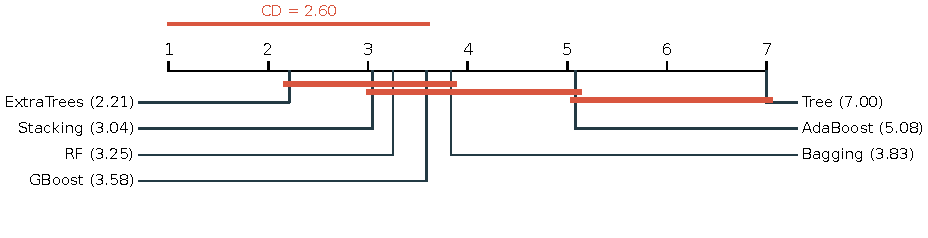
\includegraphics[width=\textwidth]{ch02/cd_ensembles}
\caption{Critical difference diagram of seven methods on twelve data sets (AUC, 5-fold CV;
Nemenyi test, $\alpha=0.05$). Methods joined by a bar are not significantly different.}
\label{fig:cdens}
\end{figure}

% ---------------------------------------------------------------------
\section{Drawbacks}\label{sec:drawbacks}

Ensemble methods classify new examples by a combination of predictions, and this has a price:
\begin{itemize}
  \item \emph{loss of comprehensibility\index{comprehensibility|textbf}}: a single decision tree can be read and checked by an
        expert, but a vote of five hundred trees cannot. The combination can result in a
        complete loss of comprehensibility;
  \item \emph{resources}: a large amount of memory and time is required to construct, store and
        use the ensemble. The prediction throughput\index{throughput} decreases, which is relevant in real-time
        applications and on small devices (Unit~5);
  \item \emph{test costs\index{test costs|textbf}}: to predict the class of an example, most or all of its attributes
        must be measured, which is important when the attributes have costs associated with
        their tests (\cref{sec:costs}).
\end{itemize}

\subsection{Pruning ensembles}

Not all the members of an ensemble are necessary. \emph{Ensemble\index{ensemble|textbf} pruning\index{ensemble pruning|textbf}} selects a subset of the
members that is as good as, or better than, the whole ensemble \citep{margineantu1997pruning}.
\citet{zhou2002ensembling} showed that ``many could be better than all'', and ordering the members
greedily (adding at each step the member that most improves the subensemble on validation data)
and keeping only the first part of the ordering often matches or even improves the full ensemble
with a fraction of the cost \citep{martinezmunoz2009analysis}.

\subsection{Mimetic classifiers and model distillation}

Since ensembles are like black boxes, a natural idea is to use them as \emph{oracles} to train a
single comprehensible\index{comprehensibility} model that copies their behaviour. A \emph{mimetic\index{mimetic classifier|textbf} classifier}
\citep{domingos1997knowledge,estruch2003simple} is built as follows, assuming some information
about the distribution of the features:
\begin{enumerate}
  \item generate a large random data set of unlabelled examples (from the assumed feature
        distributions, or by perturbing the training examples);
  \item label it with the ensemble;
  \item learn an interpretable\index{interpretability} model (a decision tree, a set of rules) from the labelled data.
\end{enumerate}
The mimetic model has as much training data as we want, all labelled consistently by the oracle,
so it can be much better than the same kind of model learned from the original data. Mimetic
classifiers are single, short trees that are comparable in accuracy to bagging\index{bagging} and boosting in
many problems. Their quality is measured by their accuracy and by their \emph{fidelity\index{fidelity|textbf}}, the
proportion of examples on which they agree with the oracle.

\begin{pylisting}[label={lst:mimetic}]{A mimetic tree that imitates a random forest}
import numpy as np
from sklearn.datasets import make_classification
from sklearn.ensemble import RandomForestClassifier
from sklearn.tree import DecisionTreeClassifier, DecisionTreeRegressor

X, y = make_classification(n_samples=4600, n_features=8, n_informative=5, n_redundant=2,
                           flip_y=0.03, class_sep=1.0, random_state=7)
X_tr, y_tr, X_te, y_te = X[:600], y[:600], X[600:], y[600:]
oracle = RandomForestClassifier(n_estimators=300, random_state=0).fit(X_tr, y_tr)

def mimic(oracle, X, n, noise=0.3, max_leaves=32, seed=0, soft=False):
    """Learn a small tree that imitates the oracle on n synthetic examples: from its
    labels (hard targets) or from its probabilities with a regression tree (soft)."""
    rng = np.random.default_rng(seed)
    Xs = X[rng.integers(0, len(X), n)]                          # resample the inputs
    Xs = Xs + rng.normal(0, noise, Xs.shape) * X.std(axis=0)    # and perturb them
    if soft:
        tree = DecisionTreeRegressor(max_leaf_nodes=max_leaves, random_state=0)
        return tree.fit(Xs, oracle.predict_proba(Xs)[:, 1])  # the oracle's probabilities
    tree = DecisionTreeClassifier(max_leaf_nodes=max_leaves, random_state=0)
    return tree.fit(Xs, oracle.predict(Xs))                     # labels of the oracle

def labels(m, X):
    return m.predict(X) if hasattr(m, "classes_") else (m.predict(X) > 0.5).astype(int)

direct = DecisionTreeClassifier(max_leaf_nodes=32, random_state=0).fit(X_tr, y_tr)
ref = oracle.predict(X_te)
for name, m in [("random forest (oracle)", oracle), ("32-leaf tree, original data", direct),
                ("32-leaf mimetic, hard labels", mimic(oracle, X_tr, n=20000)),
                ("32-leaf mimetic, soft targets", mimic(oracle, X_tr, n=20000, soft=True))]:
    pred = labels(m, X_te)
    print(f"{name:29s} accuracy={np.mean(pred == y_te):.3f}  "
          f"fidelity={np.mean(pred == ref):.3f}")
\end{pylisting}
\begin{pyoutput}
random forest (oracle)        accuracy=0.889  fidelity=1.000
32-leaf tree, original data   accuracy=0.830  fidelity=0.896
32-leaf mimetic, hard labels  accuracy=0.859  fidelity=0.922
32-leaf mimetic, soft targets accuracy=0.833  fidelity=0.908
\end{pyoutput}

In \cref{lst:mimetic}, a tree with 32 leaves learned from the original 600 examples has an
accuracy of 0.830; the same kind of tree learned from 20,000 examples labelled by a random forest
reaches 0.859, closer to the forest itself (0.889), and agrees with it on 92\% of the test
examples. \Cref{fig:mimetic} shows that the mimetic tree beats the directly learned tree for
every number of synthetic examples; its accuracy oscillates between 0.83 and 0.86 because the
size of the tree, not the amount of data, becomes the limit.

The last line of \cref{lst:mimetic} learns the same kind of tree from the oracle's \emph{probabilities} instead
of its labels, with a regression tree whose prediction is thresholded at 0.5. These \emph{soft targets} do slightly
worse here (accuracy 0.833, fidelity 0.908), and the result holds for other seeds and for trees of 64 leaves: a small
tree spends its leaves modelling degrees of confidence inside each class rather than the boundary between them. Soft
targets pay off when the student can represent the whole distribution, as in the knowledge distillation\index{model distillation} of neural
networks described below.

\begin{figure}[htbp]
\centering
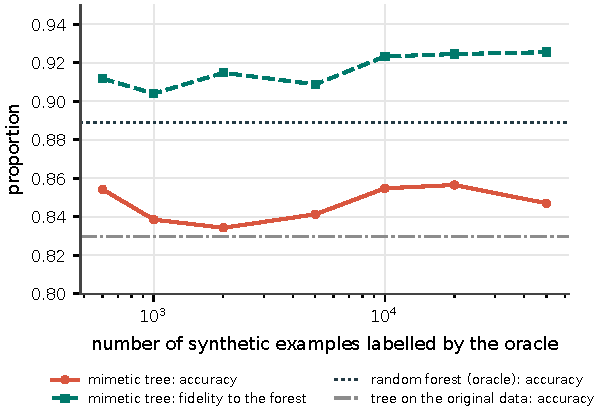
\includegraphics[width=0.74\textwidth]{ch02/mimetic}
\caption{Accuracy and fidelity of a 32-leaf mimetic tree as a function of the number of
synthetic examples labelled by a random forest, compared with the forest and with a 32-leaf tree
learned from the 600 original examples.}
\label{fig:mimetic}
\end{figure}

The same idea has been rediscovered several times. TREPAN \citep{craven1996extracting} extracted
trees from neural networks; \emph{model compression} \citep{bucila2006model} trained small neural
networks to imitate large ensembles; and \emph{knowledge distillation} \citep{hinton2015distilling}
trains a small network on the soft probabilities of a large one, and is today a standard way of
deploying large models, including language models, at a lower cost.

\subsection{Explanations, Clever Hans and security}

Imitating a model is also the basis of many \emph{explanation} methods, studied in Unit~3. LIME\index{LIME}
\citep{ribeiro2016should} explains the decision of any classifier $f$ on an example $x$ locally:
it samples perturbed examples around $x$, labels them with $f$, weights them by their proximity
to $x$ with a kernel $\pi_x$, and learns a simple (for example, sparse linear) model $g$ that
approximates $f$ well in the vicinity of $x$,
\begin{equation}
  \xi(x)=\argmin_{g\in G}\ \mathcal L(f,g,\pi_x)+\Omega(g),
\end{equation}
where $\Omega$ penalises the complexity of $g$. A mimetic\index{mimetic classifier} classifier is a \emph{global} surrogate\index{global surrogate};
LIME is a \emph{local} one.

Explanations matter because a model can be accurate for the wrong reasons. Clever Hans was a
horse that, at the beginning of the twentieth century, seemed able to do arithmetic; in fact it
was reading involuntary cues in the body language of its questioners. Ian Goodfellow compared
machine learning to Clever Hans: a model learns how to obtain its reward (for instance, a high
accuracy at labelling images), but not necessarily using the right cues. \citet{lapuschkin2019unmasking}
showed real examples: a classifier recognised horses in the PASCAL VOC images by detecting a
copyright tag present in many horse pictures, and added the label ``horse'' to a car when the tag
was pasted on its picture. In natural language processing, a model that seemed to reason about
arguments was found to exploit spurious lexical cues of the data set \citep{niven2019probing}.

This connects ensembles with security. We need to be sure that the model really learns the right
concept, which is difficult with black-box models. In software, using open-source libraries
allows anyone to inspect the code and to find and correct bugs; in machine learning this is not
always possible, since the behaviour of a model is in its parameters, not in its code. Using
comprehensible\index{comprehensibility} models where possible, studying the vulnerabilities of the most used frameworks,
and checking what models have learned are part of building reliable systems (Unit~3). Mimetic
models are also used by attackers: querying a deployed model and training a copy of it allows
its parameters to be stolen \citep{tramer2016stealing} and adversarial examples\index{adversarial example} that fool the
original to be crafted \citep{papernot2017practical}.

% ---------------------------------------------------------------------
\section{Ensembles in practice}\label{sec:enspractice}

\Cref{tab:enshyper} summarises the hyperparameters that matter most for the ensembles of this
unit. Some general recommendations:
\begin{itemize}
  \item start with a random forest (robust, few hyperparameters, OOB\index{out-of-bag estimate} estimate for free) and a
        gradient boosting\index{gradient boosting} model with early stopping\index{early stopping}; on tabular data one of them is usually
        hard to beat;
  \item tune with nested or held-out validation (\cref{sec:protocols}), never on the test data;
        and remember that, with many candidates, small differences are likely to be noise
        (\cref{sec:stats});
  \item boosted models and the averaged probabilities of forests are often miscalibrated:
        calibrate them if probabilities matter (\cref{sec:calibration});
  \item impurity-based\index{feature importance} feature importances of tree ensembles are biased towards attributes with
        many values; prefer permutation importance\index{feature importance!permutation} on held-out data \citep{strobl2007bias};
  \item if comprehensibility\index{comprehensibility}, latency\index{latency} or test costs\index{test costs} matter, consider pruning, delegation\index{delegation} or
        mimetic\index{mimetic classifier} models before deploying a large ensemble.
\end{itemize}

\begin{table}[htbp]
\centering\small
\caption{Hyperparameters that matter most in common ensembles (scikit-learn names).}\label{tab:enshyper}
\begin{tabularx}{\textwidth}{@{}>{\raggedright\arraybackslash}p{3.0cm}>{\raggedright\arraybackslash}X@{}}
\toprule
Method & Main hyperparameters and advice\\
\midrule
Bagging & \code{n_estimators} (more members usually stabilise the results, with diminishing returns); unstable base models (deep trees)\\
Random forest & \code{max_features} ($\sqrt M$ for classification); \code{n_estimators} (a few hundred);
\code{min_samples_leaf} to smooth probabilities; \code{oob_score=True} for a free estimate\\
Extra trees & as random forests; often slightly better and faster, sometimes needs more trees\\
AdaBoost & base learner depth (stumps or small trees); \code{n_estimators} and \code{learning_rate}
jointly; avoid with noisy labels\\
Gradient boosting & \code{learning_rate} (0.01--0.1) with early stopping; tree size
(\code{max_depth} or \code{max_leaf_nodes}); subsampling and regularisation\\
Stacking & diverse, reasonably good base models; simple metamodel; cross-validated meta-features\\
\bottomrule
\end{tabularx}
\end{table}

% ---------------------------------------------------------------------
\section{Summary}\label{sec:summary2}

\begin{itemize}
  \item Ensemble learning provides different methods that can improve the predictions of models.
        Combinations work when their members are both good (better than random) and diverse:
        Condorcet\index{Condorcet's jury theorem}'s theorem and the ambiguity decomposition\index{ambiguity decomposition} make this precise.
  \item Diversity\index{diversity} can be generated by manipulating the training examples, the features, the
        classes or the learning process, implicitly or explicitly, and can be measured with
        pairwise statistics and kappa--error\index{kappa--error diagram} diagrams.
  \item Predictions can be fused by averaging, multiplying, voting\index{voting}, Bayesian model averaging\index{Bayesian model averaging} or a
        learned metamodel; uniform averaging is simple and hard to beat.
  \item Bagging\index{bagging} and random forests reduce variance and degrade gracefully with label noise\index{label noise}; boosting
        reduces bias and is often more accurate on clean data, but AdaBoost\index{AdaBoost}, with its exponential loss,
        is sensitive to label noise (for gradient boosting\index{gradient boosting} it depends on the loss). Experimental
        comparisons show that random forests and boosted trees remain strong baselines on tabular data.
  \item Hybrid models (voting, stacking\index{stacking}, cascading\index{cascading}, mixtures of experts\index{mixture of experts}) combine different
        techniques and usually improve performance, provided the combination is learned on fresh
        data.
  \item A model can also know when not to predict. Abstaining is optimal when every prediction
        costs more than abstaining; for two classes, the window rule\index{window rule} of cautious classifiers\index{cautious classifier} with a
        cost-matched class bias is exactly the optimal reject rule. Cautious classifiers are
        evaluated by their accuracy--abstention\index{abstention} trade-off, which depends on how well their
        confidence ranks their own mistakes. Delegating\index{delegation} classifiers pass uncertain cases to a
        specialist, to a stronger but costlier model (a cascade) or to a person.
  \item The main drawbacks of combinations are comprehensibility\index{comprehensibility}, resources, test costs\index{test costs} and slower
        predictions; pruning, delegation and mimetic\index{mimetic classifier} models (distillation\index{model distillation}) mitigate them.
\end{itemize}

\section*{Bibliographic notes}
\phantomsection\addcontentsline{toc}{section}{Bibliographic notes}

\citet{kuncheva2014combining} is the reference textbook on combining classifiers, and
\citet{zhou2012ensemble} gives a concise and modern treatment of ensemble methods with their theory;
\citet{kyriakides2019hands} is a practical introduction in Python. \citet{dietterich2000ensemble}
remains an excellent short overview of why ensembles work, and \citet{brown2005diversity} survey the
methods for creating diversity\index{diversity}. Chapters~8, 10, 15 and~16 of \citet{hastie2009elements} cover
bagging\index{bagging}, boosting, random forests and ensemble learning from the statistical point of view. The
original papers on bagging \citep{breiman1996bagging}, boosting \citep{freund1997decision}, random
forests \citep{breiman2001random}, stacking\index{stacking} \citep{wolpert1992stacked}, cascade generalisation\index{cascading}\index{generalisation}
\citep{gama2000cascade} and mixtures of experts\index{mixture of experts} \citep{jacobs1991adaptive} are all very readable.
Cautious\index{cautious classifier} and delegating\index{delegation} classifiers are introduced in \citet{ferri2004cautious} and
\citet{ferri2004delegating}, and \citet{hendrickx2024machine} survey learning with a reject option\index{abstention};
\citet{mozannar2020consistent} and \citet{chen2023frugalgpt} are good entry points to learning to defer
and to model cascades.

\section*{Exercises}
\phantomsection\addcontentsline{toc}{section}{Exercises}

\begin{enumerate}[label=\textbf{2.\arabic*},ref=2.\arabic*,leftmargin=*,itemsep=6pt]
  \item\label{exr2:condorcet} Three independent classifiers are each right with probability 0.7.
        What is the probability that their majority vote\index{voting} is right? And for five classifiers?
  \item\label{exr2:fusion} Three models assign the probabilities $(0.70,0.25,0.05)$,
        $(0.10,0.50,0.40)$ and $(0.45,0.40,0.15)$ to the classes $(a,b,c)$. Which class is predicted
        by majority voting, by the linear combiner\index{linear combiner} and by the product combiner\index{product combiner}? Explain the
        difference.
  \item\label{exr2:bootstrap} What is the probability that a given example appears at least once
        in a bootstrap\index{bootstrap} sample of a data set with $n=10$ examples? And when $n\to\infty$?
  \item\label{exr2:variance} The members of a bagged ensemble have predictions with variance 1 and
        pairwise correlation 0.4. Compute the variance of the average of 10 members and of
        infinitely many members. What does a random forest try to change?
  \item\label{exr2:ada} In the first round of AdaBoost\index{AdaBoost} on 10 examples with uniform weights, the
        model misclassifies two examples. Compute $\varepsilon_1$, $\alpha_1$ and the new weights.
  \item\label{exr2:ambiguity} Two regression models predict 3 and 5 for an example whose target is
        4.5. Compute the ensemble error, the average error and the ambiguity\index{ambiguity decomposition}, and check
        \cref{eq:ambiguity}.
  \item\label{exr2:cautious} A cautious\index{cautious classifier} binary classifier gives the following matrix on 200 examples
        (rows: predicted $+$, $-$, $\perp$; columns: actual $+$, $-$): $(70,5)$, $(8,90)$,
        $(12,15)$. Compute coverage\index{coverage}, abstention\index{abstention}, accuracy and error, and check the relation between
        them.
  \item\label{exr2:rule} Apply the decision rule\index{decision rules} of \cref{sec:cautious} with $K=(0.6,0.4)$ and
        $w=0.5$ to the probability vectors $(0.9,0.1)$, $(0.7,0.3)$, $(0.55,0.45)$ and $(0.2,0.8)$.
  \item\label{exr2:chow} Abstaining costs 0.2 and an error costs 1. Should a calibrated classifier
        that predicts $(0.75,0.25)$ abstain? From which maximum probability is predicting better?
  \item\label{exr2:costcautious} With the cost matrix\index{cost matrix} of \cref{ex:costcautious}, what is the best
        decision for an example with probabilities $(0.2,0.3,0.5)$?
  \item\label{exr2:delegation} In a two-step delegation\index{delegation}, the first classifier keeps 70\% of the
        test examples with an accuracy of 0.95, and the second classifies the remaining 30\% with an
        accuracy of 0.75. What is the overall accuracy?
  \item\label{exr2:rebound} Continue Exercise~\ref{exr2:delegation}. The second classifier is
        confident on two thirds of the delegated examples (20\% of the total), where its accuracy
        is 0.85; on the remaining 10\% its accuracy is 0.55, whereas the first classifier would be
        right on 65\% of them. Check that the accuracy of the second classifier on all the
        delegated examples is 0.75, and compute the overall accuracy with and without round
        rebound\index{round rebound}. When does round rebound help?
  \item\label{exr2:window} False positives cost 1, false negatives cost 3 and abstaining costs
        0.4. Compute the optimal abstention band, the cost threshold $t^\star$ and the window
        $w^\star$ that makes the window rule\index{window rule} optimal, and check that the window rule abstains on
        the same band.
  \item\label{exr2:stacking} Explain why the metamodel of stacking\index{stacking} must be trained on out-of-fold
        predictions. What would happen if one of the base models were a 1-nearest neighbour\index{k-nearest neighbours@$k$-nearest neighbours}
        classifier and the metamodel were trained on its predictions on the training data?
  \item\label{exr2:mimetic} When can a mimetic\index{mimetic classifier} tree with lower accuracy than the ensemble still be
        preferable? Which quantity would you report besides its accuracy?
  \item\label{exr2:design} A fraud detection system must answer in less than 5 milliseconds, but the
        best model is a stacking of three large ensembles. Propose three ways of deploying something
        close to it within the time budget.
\end{enumerate}

\section*{Solutions to selected exercises}
\phantomsection\addcontentsline{toc}{section}{Solutions to selected exercises}

\begin{description}[font=\bfseries,leftmargin=0pt,itemsep=5pt]
  \item[\ref{exr2:condorcet}] $0.7^3+3\cdot0.7^2\cdot0.3=0.343+0.441=0.784$. For five classifiers,
        $10\cdot0.7^3\cdot0.3^2+5\cdot0.7^4\cdot0.3+0.7^5=0.309+0.360+0.168=0.837$.
  \item[\ref{exr2:fusion}] Votes: $a$, $b$, $a$, so voting\index{voting} predicts $a$. Average:
        $(0.417,0.383,0.200)$, so $a$. Normalised product: the products are $0.0315$, $0.050$ and
        $0.003$, so $b$: the low probability that the second model gives to $a$ acts as a veto.
  \item[\ref{exr2:bootstrap}] $1-(1-1/10)^{10}=1-0.349=0.651$; when $n\to\infty$, $1-e^{-1}=0.632$.
  \item[\ref{exr2:variance}] By \cref{eq:avgvar}, $0.4+0.6/10=0.46$ for 10 members and $0.4$ for
        infinitely many. A random forest decorrelates the trees to reduce $\rho$, the term that does
        not vanish.
  \item[\ref{exr2:ada}] $\varepsilon_1=0.2$, $\alpha_1=\frac12\ln4=0.693$. Before normalising, the two
        mistakes weigh $0.1\cdot2=0.2$ and the eight correct examples $0.1\cdot0.5=0.05$; after
        normalising (total 0.8), $0.25$ and $0.0625$: the mistakes carry half of the weight.
  \item[\ref{exr2:ambiguity}] $\bar f=4$, $E=0.25$; $\bar E=(2.25+0.25)/2=1.25$;
        $\bar A=(1+1)/2=1$; and $1.25-1=0.25$.
  \item[\ref{exr2:cautious}] $\mathit{Card}=200$, 173 classified: coverage\index{coverage} $0.865$, abstention\index{abstention}
        $0.135$; accuracy $160/173=0.925$; error $13/200=0.065$. Indeed
        $0.925\cdot0.865=0.80=0.865-0.065$.
  \item[\ref{exr2:rule}] $\tau=(0.4\cdot0.5+0.6,\ 0.6\cdot0.5+0.4)=(0.8,0.7)$. $(0.9,0.1)$: class 1;
        $(0.7,0.3)$: unknown; $(0.55,0.45)$: unknown; $(0.2,0.8)$: class 2.
  \item[\ref{exr2:chow}] Abstain if $\max_ip_i<1-0.2=0.8$, so yes: predicting has expected cost\index{expected cost}
        0.25, more than 0.2. Predicting is better from a maximum probability of 0.8.
  \item[\ref{exr2:costcautious}] Expected costs: $a$: $-0.5+1.2+1.0=1.7$; $b$: $0.42-1.05=-0.63$;
        $c$: $0.24+0.39-2.0=-1.37$; $\perp$: 0. The best decision is $c$.
  \item[\ref{exr2:delegation}] $0.7\cdot0.95+0.3\cdot0.75=0.665+0.225=0.89$.
  \item[\ref{exr2:rebound}] On the delegated 30\%, the second classifier is right on
        $0.2\cdot0.85+0.1\cdot0.55=0.225$ of the total, that is, $0.225/0.3=0.75$. Without rebound the
        overall accuracy is $0.665+0.225=0.89$; with rebound, the last 10\% is classified by the
        first classifier and the accuracy is $0.665+0.2\cdot0.85+0.1\cdot0.65=0.90$. Round rebound\index{round rebound}
        helps exactly when the first classifier is more accurate than the second on the cases that
        bounce back.
  \item[\ref{exr2:window}] Band: $0.4/3=0.133<p<1-0.4=0.6$. Then $t^\star=1/4=0.25$ and
        $w^\star=1-0.4\cdot4/3=0.467$, and the window is $0.25\cdot(1-0.467)=0.133<p<0.25+0.75\cdot0.467=0.6$.
  \item[\ref{exr2:stacking}] On its own training data a 1-NN classifier is always right, so a
        metamodel trained on those predictions would learn to trust it blindly, although its
        predictions on new data are much worse. Out-of-fold predictions show the metamodel how each
        base model behaves on unseen examples.
  \item[\ref{exr2:mimetic}] When comprehensibility\index{comprehensibility}, auditability, latency or test costs\index{test costs} matter more
        than a small loss of accuracy. Report its \emph{fidelity\index{fidelity|textbf}} to the ensemble, and its size.
  \item[\ref{exr2:design}] For instance: distil\index{model distillation} the stacking\index{stacking} into a single small model (mimetic\index{mimetic classifier}
        model or distillation); prune the ensembles\index{ensemble pruning}; or use a delegating\index{delegation} cascade\index{cascading} in which a fast
        model answers the easy cases and only the uncertain ones (within the budget) go to the
        expensive model.
\end{description}


% =====================================================================
%  Unit 3 -- Reliable models
%  (this file is assembled from src/ch03/*.tex by build_chapter.py)
% =====================================================================
\chapter{Reliable Models}\label{ch:reliable}

In January 2021, the government of the Netherlands resigned over a scandal in which the tax authorities had
wrongly accused thousands of families of defrauding the system of childcare benefits, demanding that they repay
large sums and pushing many of them into debt. Among the tools that selected applications for scrutiny was a
risk-classification model that, among other indicators, took into account whether the applicant had Dutch
nationality \citep{amnesty2021xenophobic}. The model may well have been accurate by some measure; it was neither
fair, nor understandable to the people it judged, nor subject to effective human oversight.

A model can be accurate and still be unacceptable. It may treat some groups of people worse
than others, rely on spurious correlations that will not hold tomorrow, be impossible to
understand or audit, or be easy to fool by someone who wants it to fail. This unit studies four
aspects of the \emph{reliability} of models that go beyond the metrics of \cref{ch:evaluation}:
\emph{fairness\index{fairness|textbf}} (are decisions made the right way and for the right reasons?), \emph{causality\index{causality|textbf}}
(what would happen if we acted?), \emph{interpretability\index{interpretability|textbf}} (can we understand why a model
decides what it decides?) and \emph{security} (can the model withstand an adversary?). The four
are closely connected: we need causal reasoning to talk about discrimination, explanations to
detect unfairness and vulnerabilities, and an understanding of attacks to trust explanations. We close with
the European AI Act\index{AI Act}, which turns many of these concerns into legal obligations.

\begin{objectives}
After studying this unit you should be able to:
\begin{itemize}
  \item recognise the sources of unfairness along the life cycle of a data-driven decision
        system (measurement, learning, action and feedback);
  \item define and compute the main group fairness criteria (independence, separation\index{fairness!separation} and
        sufficiency\index{fairness!sufficiency}), explain why they are generally incompatible, and know the techniques that
        enforce them;
  \item reason with structural causal models\index{structural causal model}: distinguish conditioning from intervening,
        identify confounders\index{confounder}, mediators\index{mediator} and colliders\index{collider}, apply the adjustment formula, and compute
        counterfactuals\index{counterfactual};
  \item explain why interpretability matters, classify interpretability methods, and interpret
        linear models, logistic regression\index{logistic regression}, trees and rules;
  \item apply model-agnostic methods (partial dependence\index{partial dependence plot}, ICE\index{individual conditional expectation}, interaction strength,
        permutation importance\index{feature importance!permutation}, surrogates\index{global surrogate}, LIME\index{LIME} and Shapley\index{Shapley values} values) and example-based
        explanations (counterfactuals, prototypes\index{prototypes and criticisms} and criticisms, influential instances\index{influential instance}),
        knowing their limitations;
  \item describe the main attacks on machine learning systems (poisoning\index{poisoning attack}, evasion\index{evasion attack}, transfer)
        and the defensive measures, with their limits.
  \item explain the risk-based approach of the European AI Act, and relate the obligations for high-risk\index{AI Act!high-risk systems}
        systems to the techniques of this book.
\end{itemize}
\end{objectives}

% =====================================================================
\section{Fairness in machine learning}\label{sec:fairness}

\subsection{Why fairness?}

Data-driven decisions promise to be better than decisions based on intuition: they take the
available evidence into account, they can be checked, and machine learning can uncover
relevant factors that people would overlook. But learning from examples is induction, and
induction is only as reliable as its examples: they must be sufficient, diverse and well
annotated. If the examples reflect historical prejudices, a model learned from them will
reproduce those prejudices, often in a way that is harder to see.

Disparities do not require bad intentions. In 2016, an analysis of a same-day delivery service
of a large online retailer found that, in several US cities, the neighbourhoods selected for the
service were disproportionately white \citep{ingold2016amazon}. We do not know how that system
works, nor whether it uses machine learning; but the example shows how a decision that seems
neutral (``offer the service where it is profitable'') can produce stark demographic
differences. Whether a disparity amounts to \emph{discrimination} depends on whether it is
justified and whether it is harmful, questions that rarely have simple answers and on which
philosophy, law and sociology have much to say \citep{barocas2023fairness}.

\subsection{The machine learning loop}

Unfairness can enter at every stage of a system that produces decisions with machine learning
(\cref{fig:mlloop}).

\begin{figure}[htbp]
\centering
\begin{tikzpicture}[font=\small\sffamily,
  st/.style={draw=edmnavy,fill=edmnavy!6,rounded corners=3pt,minimum width=26mm,minimum height=9mm,align=center},
  arr/.style={-{Stealth[length=2.2mm]},edmnavy,thick}]
  \node[st] (w) at (0,0) {world\\(individuals)};
  \node[st] (d) at (5,0) {data};
  \node[st] (m) at (10,0) {model};
  \node[st] (a) at (5,-2.3) {actions\\(decisions)};
  \draw[arr] (w) -- node[above,font=\scriptsize\sffamily] {measurement} (d);
  \draw[arr] (d) -- node[above,font=\scriptsize\sffamily] {learning} (m);
  \draw[arr] (m) |- node[pos=0.25,right,font=\scriptsize\sffamily] {prediction} (a);
  \draw[arr] (a) -| node[pos=0.75,left,font=\scriptsize\sffamily] {impact} (w);
  \draw[arr,dashed,edmcoral] (a) -- node[right,font=\scriptsize\sffamily,text=edmcoral] {feedback} (d);
\end{tikzpicture}
\caption{The stages of a machine learning system that makes decisions about people. Each
arrow is a possible source of unfairness.}
\label{fig:mlloop}
\end{figure}

\paragraph{Measurement} Turning the world into data requires subjective decisions and is full of
technical difficulties. The target variable is often a construct that cannot be measured
directly (``creditworthiness'', ``a good employee'') and is replaced by a measurable proxy\index{proxy variable},
whose biases the model will inherit. A widely used algorithm for allocating extra care to
patients in the United States predicted future health \emph{costs} as a proxy for health
\emph{needs}; because less money had historically been spent on Black patients with the same
needs, the algorithm systematically underestimated their needs \citep{obermeyer2019dissecting}.
Variables recorded by decision makers (who was granted bail, who was arrested) measure their
decisions as much as the underlying phenomenon, and data sets repurposed from another use carry
the choices of their original creators. Knowing the \emph{provenance} of the data is crucial.

\paragraph{Learning} A learning algorithm can preserve, mitigate or exacerbate the disparities in
its data, and it has no general way of telling legitimate patterns from stereotypes. Minority
groups are, by definition, represented by fewer examples, so their patterns are learned less
accurately, and the desire to avoid overfitting\index{overfitting} can make the algorithm treat genuine differences
as noise. A single accuracy\index{accuracy} figure hides these differences: commercial face analysis systems
that were very accurate on average had error rates\index{error rate} many times higher for darker-skinned women
than for lighter-skinned men \citep{buolamwini2018gender}.

\paragraph{Action} A prediction is not a decision. Predicting who will fail a course is
different from deciding what to do about it, and decisions that are fairly rendered under unfair
circumstances may do little to improve people's lives. Moreover, the errors of a model may be
unequally distributed between groups, so that the cost of the mistakes falls on some people more
than on others.

\paragraph{Feedback} Decisions change the world that produces the next data. Predictions can be
\emph{self-fulfilling}: if police are sent where the model predicts crime, more crime is recorded
there, which confirms the prediction \citep{ensign2018runaway}. Recommendations determine which
items users can click, and hence the training data\index{training set} of the next model; and predictions can change
the phenomenon they predict (a route predicted to be fast attracts traffic and stops being fast).
Feedback from users can also carry cultural prejudices, for instance when performance reviews
are used as a target.

\paragraph{Other ethical considerations} Training data must be diverse enough for the
population the system will serve, and systems can perpetuate stereotypes: word embeddings\index{embedding} learned
from text associate occupations with genders in ways that reflect, and can reinforce, social
stereotypes \citep{bolukbasi2016man}.

\begin{keyidea}
There are reasons to be cautiously optimistic: data-driven decision making forces us to
articulate the objectives of a decision, makes the decision process more transparent and
auditable than many human decisions, and allows effective intervention\index{intervention}. But fairness\index{fairness} cannot be
reduced to an algorithmic stamp of approval. The value of the formal tools of this section is
that they make it harder to avoid the difficult questions.
\end{keyidea}

% ---------------------------------------------------------------------
\section{Fairness criteria for classification}\label{sec:fairnesscriteria}

We consider a classification problem with features $X$, a target $Y$ and a \emph{sensitive
attribute\index{protected attribute|textbf}} $A$ (gender, ethnicity, age, religion\dots) that defines the groups whose treatment we
want to compare. The classifier is usually a \emph{score} $R=r(X)$, a single number that
summarises the features, turned into a decision by a threshold\index{threshold} (\cref{sec:roc}).

\subsection{No fairness through unawareness}

The first intuition is to remove $A$ from the features. It does not work. In large feature
spaces sensitive attributes\index{protected attribute} are generally \emph{redundantly encoded}: they can be predicted from
the other features (place of residence, shopping habits, browsing history, even genetic markers),
and a model that does not see $A$ can still treat the groups very differently. Removing the
sensitive attribute can even be harmful, for instance in medicine, where a variable such as sex
or ethnicity may be needed to give everyone an accurate prediction.

\Cref{lst:unawareness} uses the synthetic credit data of \cref{sec:creditcase}. The features
(income, debt and a ``zip code'' that summarises the neighbourhood) predict the group of an
applicant with an AUC\index{area under the ROC curve (AUC)} of 0.967. A logistic regression trained \emph{without} $A$ accepts 41\% of
the applicants of group $a$ and 13\% of those of group $b$, and it gives a negative weight to the
zip code, which acts as a proxy\index{proxy variable} of the group. Removing the zip code changes little (40\% against
16\%), because income and debt also differ between the groups.

\begin{pylisting}[label={lst:unawareness}]{Removing the sensitive attribute does not remove its influence}
import numpy as np
from sklearn.linear_model import LogisticRegression
from sklearn.metrics import roc_auc_score
from sklearn.model_selection import cross_val_predict, train_test_split
from credit import credit_data

# X = (income, debt, zipcode); A is not in X
X, A, Y = credit_data(40000)
pA = cross_val_predict(LogisticRegression(), X, A, cv=5, method="predict_proba")[:, 1]
print(f"AUC of predicting the group from the features: {roc_auc_score(A, pA):.3f}")

X_tr, X_te, A_tr, A_te, Y_tr, Y_te = train_test_split(X, A, Y, test_size=0.5,
                                                      random_state=0)
for cols, name in [([0, 1, 2], "income, debt, zipcode"), ([0, 1], "income, debt")]:
    m = LogisticRegression().fit(X_tr[:, cols], Y_tr)
    accept = m.predict_proba(X_te[:, cols])[:, 1] >= 0.8         # lend if P(repay) >= 0.8
    print(f"{name:21s} weights={np.round(m.coef_[0], 2)}  "
          f"acceptance a={accept[A_te == 0].mean():.2f} b={accept[A_te == 1].mean():.2f}")
print(f"repayment rate: a={Y[A == 0].mean():.2f}  b={Y[A == 1].mean():.2f}")
\end{pylisting}
\begin{pyoutput}
AUC of predicting the group from the features: 0.967
income, debt, zipcode weights=[ 0.49 -0.17 -0.13]  acceptance a=0.41 b=0.13
income, debt          weights=[ 0.5  -0.17]  acceptance a=0.40 b=0.16
repayment rate: a=0.70  b=0.50
\end{pyoutput}

\subsection{Three formal criteria}

Most formal non-discrimination criteria are properties of the joint distribution of the
sensitive attribute\index{protected attribute} $A$, the target $Y$ and the score $R$, and they fall into three groups, each a
(conditional) independence statement \citep{barocas2023fairness} (\cref{tab:faircriteria}).

\begin{table}[htbp]
\centering\small
\caption{The three families of group fairness criteria.}\label{tab:faircriteria}
\begin{tabularx}{\textwidth}{@{}llX@{}}
\toprule
Criterion & Independence & In a binary classifier\\
\midrule
Independence & $R\perp A$ & equal acceptance rates (demographic parity)\\
Separation & $R\perp A\mid Y$ & equal true positive and false positive rates (equalised odds)\\
Sufficiency & $Y\perp A\mid R$ & equal predictive values; calibration by group\\
\bottomrule
\end{tabularx}
\end{table}

\paragraph{Independence} The score must be independent of the sensitive attribute. For a binary
decision this means that the probability of a positive decision is the same in all groups,
$P\{R=1\mid A=a\}=P\{R=1\mid A=b\}$, a criterion known as \emph{demographic} or
\emph{statistical parity\index{fairness!demographic parity|textbf}}. It can be relaxed to a maximum difference,
$P\{R=1\mid A=a\}\geq P\{R=1\mid A=b\}-\epsilon$, or to a ratio: the ``four-fifths rule'' of US
employment law considers a selection rate of a group below 80\% of that of the most favoured group
as evidence of adverse impact \citep{feldman2015certifying}. For scores, independence can be
measured by the mutual information $I(A;R)=H(A)+H(R)-H(A,R)$, which is zero under independence.

Independence has important limitations. It can be satisfied in undesirable ways: a lender could
accept the most solvent applicants of one group and a random selection of the same size of the
other, which equalises the rates while being careless with the second group. And when the target
is genuinely correlated with the group, a perfect classifier violates it. There are three families
of techniques to achieve it (and, adapted, the other criteria): \emph{pre-processing}, which
adjusts the data or the feature space so that it is uncorrelated with the sensitive attribute
(for instance, by reweighting the examples, \citealp{kamiran2012data}); \emph{in-processing},
which adds a fairness\index{fairness} constraint or penalty to the optimisation problem of the learner
\citep{zafar2017fairness,agarwal2018reductions}; and \emph{post-processing}, which adjusts a
learned classifier, typically with group-specific thresholds.

\paragraph{Separation} Often the sensitive attribute is correlated with the target, and part of
the correlation is legitimate. Separation\index{fairness!separation} allows the score to depend on $A$ only through the
target: $R\perp A\mid Y$. For a binary classifier,
\begin{align}
  P\{R=1\mid Y=1,A=a\}&=P\{R=1\mid Y=1,A=b\},\\
  P\{R=1\mid Y=0,A=a\}&=P\{R=1\mid Y=0,A=b\},
\end{align}
that is, equal true positive rates\index{true positive rate} and equal false positive rates\index{false positive rate} in all groups
(\emph{equalised odds\index{fairness!equalised odds|textbf}}): the errors of the classifier are equally distributed. A common
relaxation requires only one of the two equalities, for instance equal true positive rates
(\emph{equality of opportunity\index{fairness!equal opportunity|textbf}}, \citealp{hardt2016equality}). Separation can be achieved by
post-processing without retraining, using the ROC curves\index{ROC curve} of \cref{sec:roc}: each group has its
own ROC curve, and the achievable operating points\index{operating point} that satisfy separation are those in the
intersection of the regions under the group curves; the decision maker picks the cheapest one,
possibly randomising between two thresholds \citep{hardt2016equality}.

\paragraph{Sufficiency} The score must capture everything that the group says about the target,
$Y\perp A\mid R$: once the score is known, the group adds no information,
\begin{equation}
  P\{Y=1\mid R=r,A=a\}=P\{Y=1\mid R=r,A=b\}.
\end{equation}
For a binary classifier this means equal positive and negative predictive values\index{predictive value!negative} in all groups.
For a probabilistic score it is closely related to \emph{calibration\index{calibration|textbf} by group},
$P\{Y=1\mid R=r,A=a\}=r$ for all groups $a$ (\cref{sec:calibration}). An unconstrained model that fits the data
well often comes close to calibration in the groups it can identify, but this depends on the learner,
its capacity, the information available and the data, and it must be checked.

\Cref{lst:fairmetrics} computes the three criteria for the credit model with the profit-optimal
threshold of 0.8. In both groups the mean score equals the repayment rate within 0.002, which checks calibration
only on average; the reliability curves of \cref{fig:fairnesscredit}c stay close to the diagonal across
score levels, so the \emph{score} is approximately calibrated by group. The \emph{decision} is another
matter: its positive predictive values\index{predictive value!positive} are similar (0.90 and 0.86), but its negative predictive values
are not (0.44 and 0.55), so the thresholded decision does not satisfy sufficiency\index{fairness!sufficiency}: thresholding a
calibrated score need not preserve it. Independence is far from holding: the acceptance rate of group $b$ is 32\% of that of
group $a$, well below four fifths. Separation does not hold either: the true positive rate, the
fraction of applicants who would repay that get a loan, is 0.53 in group $a$ and only 0.23 in
group $b$.

\begin{pylisting}[label={lst:fairmetrics}]{Independence, separation and sufficiency of a credit score}
import numpy as np
from sklearn.linear_model import LogisticRegression
from sklearn.model_selection import train_test_split
from credit import credit_data

X, A, Y = credit_data(40000)
X_tr, X_te, A_tr, A_te, Y_tr, Y_te = train_test_split(X, A, Y, test_size=0.5,
                                                      random_state=0)
R = LogisticRegression().fit(X_tr, Y_tr).predict_proba(X_te)[:, 1]   # score (A not used)
D = R >= 0.8                                                          # decision: lend
for g, name in [(0, "a"), (1, "b")]:
    m = A_te == g
    gap = R[m].mean() - Y_te[m].mean()  # calibration-in-the-large
    print(f"group {name}: base={Y_te[m].mean():.2f} accept={D[m].mean():.2f} "
          f"TPR={D[m & (Y_te == 1)].mean():.2f} FPR={D[m & (Y_te == 0)].mean():.2f} "
          f"score-base={gap:+.3f}")
    print(f"         PPV={Y_te[m & D].mean():.2f} NPV={1 - Y_te[m & ~D].mean():.2f}"
          f"  (predictive values of the decision)")
print(f"demographic parity ratio b/a = {D[A_te == 1].mean() / D[A_te == 0].mean():.2f}")
\end{pylisting}
\begin{pyoutput}
group a: base=0.70 accept=0.41 TPR=0.53 FPR=0.14 score-base=-0.002
         PPV=0.90 NPV=0.44  (predictive values of the decision)
group b: base=0.50 accept=0.13 TPR=0.23 FPR=0.04 score-base=-0.001
         PPV=0.86 NPV=0.55  (predictive values of the decision)
demographic parity ratio b/a = 0.32
\end{pyoutput}

\subsection{The criteria are incompatible}

These criteria cannot, in general, be satisfied simultaneously \citep{kleinberg2017inherent,chouldechova2017fair}:
\begin{itemize}
  \item independence and sufficiency\index{fairness!sufficiency} are mutually exclusive when $A$ and $Y$ are not independent;
  \item independence and separation\index{fairness!separation} are mutually exclusive when $A$ and $Y$ are not independent
        and the score is informative ($R$ is not independent of $Y$);
  \item separation and sufficiency together lead to degenerate solutions unless the groups have
        the same base rates or the classifier is perfect.
\end{itemize}
The last incompatibility follows from an identity that relates the error rates\index{error rate} of a binary
classifier in a group with prevalence\index{prevalence} $p=P\{Y=1\}$ \citep{chouldechova2017fair}:
\begin{equation}\label{eq:chouldechova}
  \FPR=\frac{p}{1-p}\cdot\frac{1-\PPV}{\PPV}\cdot\TPR .
\end{equation}
If two groups have different prevalences, equal predictive values (sufficiency) and equal true
positive rates\index{true positive rate} force different false positive rates\index{false positive rate}. In \cref{lst:fairmetrics}, group $a$ has
$p=0.70$, $\PPV=0.90$ and $\TPR=0.53$, which gives $\FPR=\frac{0.7}{0.3}\cdot\frac{0.1}{0.9}\cdot0.53
\approx0.14$, while group $b$, with $p=0.50$, has $\FPR\approx0.04$. Choosing a criterion is
therefore a choice about which errors, and whose, matter most.

\subsection{The limits of observational criteria}

All the criteria above are \emph{observational}: they depend only on the joint distribution of
$(A,Y,R)$ and the features. Two scenarios with very different mechanisms can produce exactly the
same distribution. Imagine a model that predicts whether someone is a software engineer. In one
scenario, its features are visits to a website popular among one gender and to a code-hosting
platform; in the other, whether the person studied computer science and attended a conference for
women in computing. Both kinds of features can be correlated with gender in the same way, so any
observational criterion gives the same verdict in both cases, although we may judge them very
differently. Observational criteria cannot tell us whether a classifier uses the sensitive
attribute\index{protected attribute}, nor evaluate alternatives to the data we have. To go further we need to reason about
how the data were generated: measurement and causality\index{causality} (\cref{sec:causality}).

\begin{pitfall}
A fairness\index{fairness} criterion is a diagnostic, not a certificate. We cannot base a conclusive argument
of fairness or unfairness on the value of a single observational criterion; and the criteria can
be manipulated by changing the real-world processes that the data reflect, sometimes in harmful
ways.
\end{pitfall}

% ---------------------------------------------------------------------
\section{Case study: credit scoring}\label{sec:creditcase}

A bank decides whether to grant a loan to each applicant based on a score $R$, the predicted
probability of repayment. A repaid loan earns 1 unit and a default costs 4 units, so the
profit-maximising decision is to lend when $R\geq0.8$ (\cref{sec:costs}). The applicants belong to
two groups: group $b$, 30\% of the population, has a lower average creditworthiness for
historical reasons, and its repayment rate is 50\% against 70\% in group $a$. The data are
synthetic (\cref{lst:credit}), which lets us know exactly how they were generated.

\begin{pylisting}[label={lst:credit}]{Synthetic credit data and four lending policies}
"""Synthetic credit-scoring data and four lending policies (Unit 3)."""
import numpy as np

def credit_data(n, seed=0):
    """Two groups of applicants; group b (A=1, 30%) is less creditworthy on average."""
    rng = np.random.default_rng(seed)
    A = (rng.random(n) < 0.3).astype(int)
    z = rng.normal(0, 1, n) - 0.8 * A                       # latent creditworthiness
    Y = (rng.random(n) < 1 / (1 + np.exp(-(1.5 * z + 1.2)))).astype(int)   # 1 = repays
    income = 2.0 * z + rng.normal(0, 1, n)
    debt = -1.0 * z + rng.normal(0, 1.2, n)
    zipcode = 1.5 * A + rng.normal(0, 0.6, n)               # neighbourhood: a proxy of A
    return np.c_[income, debt, zipcode], A, Y

GAIN, LOSS = 1.0, 4.0                    # profit of a repaid loan, loss of a default

def profit(R, A, Y, t):
    """Profit of accepting the applicants whose score reaches their group's threshold."""
    accept = R >= np.asarray(t)[A]
    return GAIN * np.sum(accept & (Y == 1)) - LOSS * np.sum(accept & (Y == 0))

def four_policies(R, A, Y):
    """Thresholds (group a, group b) of four lending policies, each maximising profit."""
    grid = np.quantile(R, np.linspace(0, 1, 401))           # candidate thresholds
    rates = np.linspace(0.005, 0.995, 199)                  # candidate common rates
    best = lambda cands: max(cands, key=lambda t: profit(R, A, Y, t))
    # threshold accepting a fraction r
    q = lambda mask, r: np.quantile(R[mask], 1 - r)

    # best threshold within one group
    def group_best(g):
        m = A == g
        return max(grid, key=lambda s: profit(R[m], np.zeros(m.sum(), int), Y[m], (s,)))

    return {"max profit": (group_best(0), group_best(1)),
            "single threshold": best([(s, s) for s in grid]),
            "independence": best([(q(A == 0, r), q(A == 1, r)) for r in rates]),
            "equal opportunity": best([(q((A == 0) & (Y == 1), r),
                                       q((A == 1) & (Y == 1), r)) for r in rates])}
\end{pylisting}

The bank compares four lending policies, each maximising profit subject to a different
constraint, by choosing one threshold per group \citep{barocas2023fairness}:
\begin{itemize}
  \item \emph{maximum profit}: possibly different thresholds for each group, chosen only to
        maximise profit;
  \item \emph{single threshold\index{threshold|textbf}}: the same threshold for all the groups;
  \item \emph{independence}: equal acceptance rates in all the groups;
  \item \emph{equality of opportunity\index{fairness!equal opportunity|textbf}}: equal true positive rates\index{true positive rate} in all the groups. It is half of
        separation\index{fairness!separation}, which also requires equal false positive rates\index{false positive rate} (equalized odds\index{fairness!equalised odds}).
\end{itemize}

\begin{pylisting}[label={lst:policies}]{Thresholds, rates and profit of the four lending policies}
import numpy as np
from sklearn.linear_model import LogisticRegression
from sklearn.model_selection import train_test_split
from credit import credit_data, four_policies, profit

X, A, Y = credit_data(40000)
X_tr, X_te, A_tr, A_te, Y_tr, Y_te = train_test_split(X, A, Y, test_size=0.5,
                                                      random_state=0)
X_va, X_te, A_va, A_te, Y_va, Y_te = train_test_split(X_te, A_te, Y_te, test_size=0.5,
                                                      random_state=1)
model = LogisticRegression().fit(X_tr, Y_tr)
R_va, R = model.predict_proba(X_va)[:, 1], model.predict_proba(X_te)[:, 1]
policies = four_policies(R_va, A_va, Y_va)       # thresholds chosen on validation
# ... and evaluated, held fixed, on the test data
top = profit(R, A_te, Y_te, policies["max profit"])
print("test data         thresholds  acceptance    TPR         FPR      profit")
for name, t in policies.items():
    acc = R >= np.asarray(t)[A_te]
    rate = lambda m: f"{acc[m & (A_te == 0)].mean():.2f} {acc[m & (A_te == 1)].mean():.2f}"
    print(f"{name:17s} {t[0]:.2f} {t[1]:.2f}   {rate(Y_te >= 0)}    {rate(Y_te == 1)}   "
          f"{rate(Y_te == 0)}   {profit(R, A_te, Y_te, t) / top:.1%}")
\end{pylisting}
\begin{pyoutput}
test data         thresholds  acceptance    TPR         FPR      profit
max profit        0.80 0.79   0.41 0.15    0.53 0.25   0.15 0.05   100.0%
single threshold  0.80 0.80   0.41 0.14    0.53 0.24   0.15 0.04   99.6%
independence      0.86 0.67   0.27 0.31    0.36 0.48   0.07 0.13   78.6%
equal opportunity 0.84 0.67   0.33 0.30    0.42 0.47   0.10 0.13   81.6%
\end{pyoutput}

The thresholds are chosen on validation data\index{validation set} and then held fixed on a separate test set\index{test set}, whose
results \cref{lst:policies} and \cref{fig:fairnesscredit} show. Because the score is calibrated in
both groups, the maximum-profit thresholds are practically the same (0.80 and 0.79) and the single
threshold loses only 0.4\% of the profit; both accept 41\% of group $a$ and 14--15\% of group $b$.
Independence, which equalised the acceptance rates on the validation data, raises the threshold of
group $a$ to 0.86 and lowers that of group $b$ to 0.67. On the test data the acceptance rates are 27\%
and 31\%, close but not equal, as must be expected on new data; the policy costs 21\% of the profit,
and group $b$ now receives loans that are more likely to default (its false positive rate rises from
0.04 to 0.13). Equality of opportunity gives true positive rates of 0.42 and 0.47 on the test data and
costs 18\% of the profit. It constrains only the true positive rates: full separation would also
equalise the false positive rates (0.10 and 0.13 here), which may require randomised decisions
\citep{hardt2016equality}. In a real bank, moreover, repayment is observed only for the loans that
were granted, while the simulation knows the outcome of every applicant.

\begin{figure}[htbp]
\centering
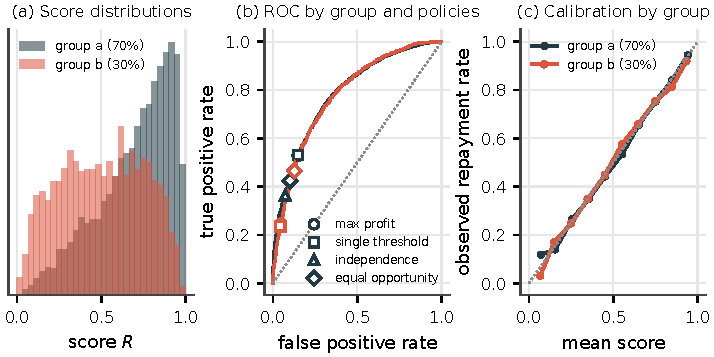
\includegraphics[width=\textwidth]{ch03/fairness_credit}
\caption{The credit-scoring case study, on test data. (a) Distribution of the score in each group.
(b) ROC curve of each group with the operating points of the four policies, whose thresholds were
chosen on validation data. (c) The score is calibrated
in both groups (sufficiency).}
\label{fig:fairnesscredit}
\end{figure}

What is the purpose of a fairness\index{fairness} criterion here? Independence would lend at the same rate in
both groups, regardless of the individuals' ability to repay, and loans that end in default can
harm the people who receive them. Imposing a criterion on a one-shot decision can even make things
worse in the long run for the group it aims to protect \citep{liu2018delayed}; directly optimising
the long-term benefit of the decisions may be a more effective intervention\index{intervention}. An alternative view
is that the criteria have \emph{diagnostic} value: the different true positive rates in our
example show that creditworthy members of group $b$ bear a much higher cost of the classification
(they are refused credit more often), a cost that is not reflected in the profit function that
the bank optimised.

% ---------------------------------------------------------------------
\section{Causality}\label{sec:causality}

Causal reasoning is a conceptual and technical framework for questions about the effect of
hypothetical actions or interventions\index{intervention}: what would happen if we did something, and which action
caused an event? Causal inference\index{causality} gives us a formal language to ask these questions, but it does
not make it easy to choose the right question, nor does it trivialise finding and interpreting the
answer. In the context of fairness\index{fairness}, causality serves three purposes: to understand the limitations
of observational criteria, to design interventions that achieve a desired effect, and to reason
about discrimination, which is itself a causal notion (\emph{because of} their sex, their
ethnicity\dots).

\subsection{The limits of observation}

In 1973 the University of California, Berkeley, admitted 44\% of the 8442 men and 35\% of the
4321 women who applied to its graduate programmes. Was there a gender bias? Admissions were
decided by each department, and \citet{bickel1975sex} looked at the departments separately.
\Cref{lst:berkeley} shows the six largest ones: women were admitted at a similar or higher rate
in four of the six, yet in aggregate the gap persists (44.5\% against 30.4\%). This reversal is an
instance of \emph{Simpson\index{Simpson's paradox|textbf}'s paradox} \citep{simpson1951interpretation}.

\begin{pylisting}[label={lst:berkeley}]{Simpson's paradox in the Berkeley admissions data}
import pandas as pd

# Six largest departments, UC Berkeley 1973 (Bickel et al., 1975)
d = pd.DataFrame({"dept": list("ABCDEF"),
                  "men": [825, 560, 325, 417, 191, 373],
                  "men_adm": [512, 353, 120, 138, 53, 22],
                  "women": [108, 25, 593, 375, 393, 341],
                  "women_adm": [89, 17, 202, 131, 94, 24]})
d["men_rate"], d["women_rate"] = d.men_adm / d.men, d.women_adm / d.women
cols = ["dept", "men", "men_rate", "women", "women_rate"]
print(d[cols].round(2).to_string(index=False))
print(f"aggregate:   men {d.men_adm.sum() / d.men.sum():.3f}   "
      f"women {d.women_adm.sum() / d.women.sum():.3f}")
w = (d.men + d.women) / (d.men + d.women).sum()          # department mix of all applicants
men_adj, women_adj = (w * d.men_rate).sum(), (w * d.women_rate).sum()
print(f"adjusted:    men {men_adj:.3f}   women {women_adj:.3f}")
\end{pylisting}
\begin{pyoutput}
dept  men  men_rate  women  women_rate
   A  825      0.62    108        0.82
   B  560      0.63     25        0.68
   C  325      0.37    593        0.34
   D  417      0.33    375        0.35
   E  191      0.28    393        0.24
   F  373      0.06    341        0.07
aggregate:   men 0.445   women 0.304
adjusted:    men 0.387   women 0.430
\end{pyoutput}

The explanation is that women applied more often to departments with low admission rates (C to
F), while men applied mostly to departments A and B, which admitted most of their applicants.
If we weight the department-specific rates by the overall distribution of applicants across
departments (the last line of the output, explained in \cref{sec:adjustment}), women's admission
rate is 43.0\% and men's 38.7\%. But the data cannot tell us \emph{why} women applied to more
competitive departments: because of their interests, because some departments advertised in ways
that discouraged women, because of a hostile climate, or for other reasons. These scenarios have
different interpretations and consequences, and they cannot be distinguished with the data at
hand. Causal models help to design new studies and to decide which variables to measure and which
to include or exclude in an analysis.

\subsection{Structural causal models}

A \emph{structural causal model\index{structural causal model|textbf}} (SCM) is a program that generates a distribution from independent
noise variables through a sequence of assignments \citep{pearl2009causality,peters2017elements}.

\begin{definition}{Structural causal model}{scm}
A structural causal model $M$ consists of variables $X_1,\dots,X_d$ and assignments
\begin{equation}
  X_i:=f_i(P_i,U_i),\qquad i=1,\dots,d,
\end{equation}
where $P_i\subseteq\{X_1,\dots,X_d\}$ are the \emph{parents} (direct causes) of $X_i$ and the
\emph{noise variables} $U_1,\dots,U_d$ are jointly independent exogenous factors. The \emph{causal
graph\index{causal graph|textbf}} has one node per variable and an edge from each parent to its child; we assume it is
acyclic. Executing the assignments in order generates a joint distribution $P_M$.
\end{definition}

\begin{example}{Exercise, overweight and heart disease}{heart}
An individual exercises regularly with probability 1/2. With probability 1/3 they have a latent
disposition to overweight, which manifests itself only without regular exercise; and without
exercise, heart disease occurs with probability 1/3. With $X$ the indicator of regular exercise,
$W$ of overweight and $H$ of heart disease, and independent noise $U_1\sim B(1/2)$,
$U_2\sim B(1/3)$, $U_3\sim B(1/3)$:
\begin{equation*}
  X:=U_1,\qquad W:=\begin{cases}0 & \text{if } X=1\\ U_2 & \text{otherwise}\end{cases},\qquad
  H:=\begin{cases}0 & \text{if } X=1\\ U_3 & \text{otherwise.}\end{cases}
\end{equation*}
Exercise prevents both overweight and heart disease, and without exercise the two are
independent. The probability of heart disease is $P_M\{H=1\}=1/2\cdot1/3=1/6$. Among overweight
people, who never exercise, it is $P_M\{H=1\mid W=1\}=1/3$. Does overweight cause heart disease in
this model? Replace the assignment of $W$ by $W:=1$, keeping the rest: the probability of heart
disease is still $1/6$, because $H$ does not depend on $W$ (\cref{lst:heart}). Observing that
someone is overweight tells us that their risk is higher, but making them lose weight would not
change it: overweight and heart disease share a common cause.
\end{example}

\begin{pylisting}[label={lst:heart}]{Conditioning versus intervening in the heart disease model}
import numpy as np

rng = np.random.default_rng(0)
n = 1_000_000

def heart_model(do_W=None):
    """Structural causal model: exercise X, overweight W and heart disease H."""
    U1, U2, U3 = rng.random(n) < 1 / 2, rng.random(n) < 1 / 3, rng.random(n) < 1 / 3
    X = U1
    W = np.where(X, False, U2) if do_W is None else np.full(n, do_W)
    H = np.where(X, False, U3)
    return X, W, H

X, W, H = heart_model()
print(f"P(H = 1)              = {H.mean():.3f}   (exact 1/6 = 0.167)")
print(f"P(H = 1 | W = 1)      = {H[W].mean():.3f}   (exact 1/3 = 0.333)")
_, _, H_do = heart_model(do_W=True)
print(f"P(H = 1 | do(W := 1)) = {H_do.mean():.3f}   (W does not cause H)")
\end{pylisting}
\begin{pyoutput}
P(H = 1)              = 0.167   (exact 1/6 = 0.167)
P(H = 1 | W = 1)      = 0.335   (exact 1/3 = 0.333)
P(H = 1 | do(W := 1)) = 0.167   (W does not cause H)
\end{pyoutput}

A causal model is a collection of assumptions about how variables interact. When we talk about
causes and effects \emph{in a model} we do not claim that they hold in the real world; different
models describe different hypothetical scenarios and serve as a basis for discussion.

\subsection{Causal graphs: forks, chains and colliders}

What matters in a causal graph\index{causal graph} are the paths that are present and absent. A node is a \emph{direct
cause} of its children and an \emph{indirect cause} of all its descendants. Three basic structures
(\cref{fig:structures}) determine how information flows and what happens when we condition on
(``control for'') a variable $Z$:
\begin{itemize}
  \item a \emph{fork\index{fork|textbf}} $X\leftarrow Z\rightarrow Y$: $Z$ is a common cause, a \emph{confounder\index{confounder|textbf}},
        that makes $X$ and $Y$ correlated even if neither causes the other (exercise in
        \cref{ex:heart}). Conditioning on $Z$ removes the spurious association;
  \item a \emph{chain} $X\rightarrow Z\rightarrow Y$: $Z$ is a \emph{mediator\index{mediator|textbf}} that transmits part
        of the effect of $X$. Conditioning on $Z$ removes the part of the effect that goes through
        it;
  \item a \emph{collider\index{collider|textbf}} $X\rightarrow Z\leftarrow Y$: $Z$ is a common effect. $X$ and $Y$ are
        independent, but conditioning on $Z$ \emph{creates} an association between them. Two
        unrelated diseases become negatively correlated among hospital patients, because having
        either one is enough to be admitted; and an admission test may seem uninformative when it
        is studied only among admitted students, who were selected partly because of it.
\end{itemize}

\begin{figure}[htbp]
\centering
\begin{tikzpicture}[font=\small\sffamily,
  v/.style={circle,draw=edmnavy,fill=edmnavy!8,minimum size=7mm,inner sep=0pt},
  hl/.style={v,fill=edmbronze!25,draw=edmbronze},
  arr/.style={-{Stealth[length=2mm]},edmnavy,thick}]
  \begin{scope}
    \node[v] (x) at (0,0) {$X$}; \node[v] (y) at (2,0) {$Y$}; \node[hl] (z) at (1,1.2) {$Z$};
    \draw[arr] (z) -- (x); \draw[arr] (z) -- (y); \draw[arr,dashed] (x) -- (y);
    \node at (1,-0.8) {(a) fork: $Z$ confounds};
  \end{scope}
  \begin{scope}[xshift=3.6cm]
    \node[v] (x) at (0,0) {$X$}; \node[hl] (z) at (1,1.2) {$Z$}; \node[v] (y) at (2,0) {$Y$};
    \draw[arr] (x) -- (z); \draw[arr] (z) -- (y); \draw[arr,dashed] (x) -- (y);
    \node at (1,-0.8) {(b) chain: $Z$ mediates};
  \end{scope}
  \begin{scope}[xshift=7.2cm]
    \node[v] (x) at (0,0) {$X$}; \node[v] (y) at (2,0) {$Y$}; \node[hl] (z) at (1,1.2) {$Z$};
    \draw[arr] (x) -- (z); \draw[arr] (y) -- (z);
    \node at (1,-0.8) {(c) collider};
  \end{scope}
  \begin{scope}[xshift=10.8cm]
    \node[v] (x) at (1,1.2) {$X$}; \node[v] (w) at (0,0) {$W$}; \node[v] (h) at (2,0) {$H$};
    \draw[arr] (x) -- (w); \draw[arr] (x) -- (h);
    \node at (1,-0.8) {(d) heart model};
  \end{scope}
\end{tikzpicture}
\caption{Basic causal structures. Dashed edges are possible direct effects. (d) The causal graph
of \cref{ex:heart}: exercise $X$ is a common cause of overweight $W$ and heart disease $H$.}
\label{fig:structures}
\end{figure}

\Cref{lst:adjustment} simulates the three structures with linear models in which the true effect
of $X$ on $Y$ is known. In the fork, the naive regression of $Y$ on $X$ doubles the effect (2.00
instead of 1) and adjusting for $Z$ recovers it. In the chain, the naive regression gives the
total effect (4) and adjusting for the mediator leaves only the direct effect (1). In the collider,
$X$ has no effect on $Y$ and the naive regression says so, but adjusting for $C$ creates a
spurious effect of $-0.5$.

\begin{pylisting}[label={lst:adjustment}]{Adjusting for a confounder, a mediator and a collider}
import numpy as np
from sklearn.linear_model import LinearRegression

rng = np.random.default_rng(1)
n = 100_000
coef = lambda cols, y: LinearRegression().fit(np.column_stack(cols), y).coef_[0]
noise = lambda: rng.normal(size=n)

# (a) fork: Z is a common cause of X and Y; the effect of X on Y is 1
Z = noise()
X = Z + noise()
Y = X + 2 * Z + noise()
print(f"fork:     naive {coef([X], Y):.2f}   adjusting for Z {coef([X, Z], Y):.2f}")
# (b) chain: X -> M -> Y plus a direct effect; total 1 + 2 * 1.5 = 4, direct 1
X = noise()
M = 2 * X + noise()
Y = X + 1.5 * M + noise()
print(f"mediator: naive {coef([X], Y):.2f}   adjusting for M {coef([X, M], Y):.2f}")
# (c) collider: X -> C <- Y; X has no effect on Y
X = noise()
Y = noise()
C = X + Y + noise()
print(f"collider: naive {coef([X], Y):.2f}   adjusting for C {coef([X, C], Y):.2f}")
\end{pylisting}
\begin{pyoutput}
fork:     naive 2.00   adjusting for Z 1.00
mediator: naive 4.00   adjusting for M 1.01
collider: naive 0.00   adjusting for C -0.50
\end{pyoutput}

\subsection{Interventions and the do-operator}

Structural causal models\index{structural causal model} formalise the effect of hypothetical actions. Given a model $M$, we can
replace an assignment $X:=f(P,U)$ by another one, most often a constant, $X:=x$. The resulting
model $M[X:=x]$ removes the influence of the parents of $X$, and the probability of an event $E$
after the intervention\index{intervention} is written
\begin{equation}
  P\{E\mid\mathrm{do}(X:=x)\}=P_{M[X:=x]}(E).
\end{equation}
This notation, the \emph{do-operator}, resembles a conditional probability, but an action is
fundamentally different from an observation. The \emph{causal effect} of the action $X:=x$ on $Y$
is the distribution of $Y$ in $M[X:=x]$; for a binary $X$ we usually summarise it by the
\emph{average treatment effect}
\begin{equation}
  \mathrm{ATE}=\E_{M[X:=1]}[Y]-\E_{M[X:=0]}[Y].
\end{equation}
In general $P\{Y=y\mid\mathrm{do}(X:=x)\}\neq P\{Y=y\mid X=x\}$, and we say that $X$ and $Y$ are
\emph{confounded} when the causal effect differs from the corresponding conditional probability.

\subsection{Adjustment and the backdoor criterion}\label{sec:adjustment}

When $X$ and $Y$ are confounded, the effect of an intervention\index{intervention} can sometimes be computed from
observational data. If $Z$ is the set of parents of $X$ (or, more generally, any set of variables
that satisfies the backdoor\index{backdoor criterion} criterion below), the \emph{adjustment formula} gives
\begin{equation}\label{eq:adjustment}
  P\{Y=y\mid\mathrm{do}(X:=x)\}=\sum_{z}P\{Y=y\mid X=x,Z=z\}\,P\{Z=z\}.
\end{equation}
In words, we estimate the effect separately in each stratum of $Z$ and average the results,
weighting each stratum by its share of the \emph{whole} population (not of the treated). The
``adjusted'' line of \cref{lst:berkeley} performs the same computation with $Z$ the department, but there
it is a \emph{descriptive} standardisation to a common distribution of departments: in the causal graph\index{causal graph}
of Berkeley discussed below, the department is a mediator\index{mediator} of sex, not a confounder\index{confounder}, so it is not a valid
adjustment set for the total effect.

A \emph{backdoor path} from $X$ to $Y$ is a path that starts with an edge pointing into $X$. When it is
\emph{open}, it lets information flow from $X$ to $Y$ in a non-causal way and the effect is confounded.
Conditioning on a non-collider\index{collider} on the path blocks it; a collider blocks it unless the collider or one
of its descendants is conditioned on. A set $Z$ satisfies the \emph{backdoor criterion} if it blocks every backdoor
path and contains no descendant of $X$; conditioning on it deconfounds the effect.

Two warnings apply. First, the adjustment formula is only valid in the absence of
\emph{unobserved confounding}, variables that are hard to measure or were never recorded, which
remains a major obstacle in practice. Second, it is tempting to control for as many variables as
possible in the hope of removing confounding, but controlling for mediators or colliders is
harmful (\cref{lst:adjustment}). The experimental alternative is the \emph{randomised controlled
trial}: subjects are randomly assigned to a treatment or a control group (ideally without knowing
which, both they and the staff), which removes every incoming edge into the treatment variable, so
that any difference in the outcome can be attributed to the treatment.

\subsection{Graphical discrimination analysis}

Let us return to Berkeley with a causal model with three variables: sex $A$, department choice
$Z$ and admission $Y$ (\cref{fig:berkeley}). Admission depends on the department and possibly on
sex ($Z\rightarrow Y$, $A\rightarrow Y$), and the data show that department choice depends on sex
($A\rightarrow Z$). The argument of \citet{bickel1975sex} had two parts: there is no evidence of a
\emph{direct} effect of sex on admission favouring men, and the \emph{indirect} effect through
department choice should not count as discrimination.

\begin{figure}[htbp]
\centering
\begin{tikzpicture}[font=\small\sffamily,
  v/.style={circle,draw=edmnavy,fill=edmnavy!8,minimum size=8mm,inner sep=0pt},
  arr/.style={-{Stealth[length=2mm]},edmnavy,thick}]
  \node[v] (a) at (0,0) {$A$};
  \node[v] (z) at (2.4,1.3) {$Z$};
  \node[v] (y) at (4.8,0) {$Y$};
  \node[v,dashed,draw=edmcoral,fill=edmcoral!10] (r) at (4.8,2.6) {$R$};
  \draw[arr] (a) -- node[above left,font=\scriptsize] {choice} (z);
  \draw[arr] (z) -- (y);
  \draw[arr] (a) -- node[below,font=\scriptsize] {direct effect} (y);
  \draw[arr,dashed,edmcoral] (r) -- (z);
  \draw[arr,dashed,edmcoral] (r) -- (y);
  \node[align=left,anchor=west,font=\scriptsize] at (5.5,1.2)
    {$A$: sex\\$Z$: department chosen\\$Y$: admission\\$R$: e.g.\ state of residence\\(hypothetical confounder)};
\end{tikzpicture}
\caption{A causal graph for the Berkeley admissions. If an unobserved variable $R$ influences both
department choice and admission, conditioning on $Z$ opens the path $A\rightarrow Z\leftarrow
R\rightarrow Y$ and the direct effect of $A$ can no longer be estimated by comparing admission
rates within departments.}
\label{fig:berkeley}
\end{figure}

\paragraph{Direct effect} To isolate the direct effect we must disable every path between $A$ and
$Y$ except the direct edge, which suggests holding the department fixed and comparing admission
rates within departments, as Bickel did. This is valid only if department choice and admission are
not confounded. If some other variable, say the state of residence $R$, influenced both, then $Z$
would be a collider\index{collider} on the path $A\rightarrow Z\leftarrow R\rightarrow Y$, and conditioning on it
would open a non-causal path. Assuming no such confounding\index{confounder}, the data show no direct effect of sex
against women. But the direct effect is a poor measure of discrimination on its own, since it
cannot detect discrimination that operates through other variables.

\paragraph{Indirect paths} Department choice may itself be shaped by discrimination: departments
may advertise their programmes in ways that discourage women, have a history of hostile behaviour,
or be feared to discriminate. Accepting the indirect path as non-discriminatory amounts to
asserting that all these scenarios are implausible. Seemingly innocuous mediating paths can hide
discriminatory practices: in \emph{Griggs v.\ Duke Power Co.} (1971), the US Supreme Court struck
down a requirement of a high-school diploma for jobs where it was not related to performance,
because it excluded disproportionately many Black applicants. We have to discuss carefully which
pathways count as evidence for or against discrimination. Discrimination can also be
\emph{structural}, embedded in the way society is organised, which models that describe how a
decision maker responds to information about individuals can hardly capture.

\subsection{Counterfactuals}

A fully specified structural causal model\index{structural causal model} can answer questions more delicate than the effect of
an action. ``Would I have avoided the traffic jam had I taken the other route this morning?'' is a
\emph{counterfactual\index{counterfactual|textbf}} question: it asks about an alternative to what actually happened, taking into
account what we observed.

\begin{example}{Which route?}{traffic}
Every morning we choose route 0 or 1 at random, $X:=U_X\sim B(1/2)$. A morning is slow ($Y=1$) if
it is a bad day ($U=1$, both routes are slow) or if there is an accident on the chosen route
($U_0=1$ or $U_1=1$), with $U,U_0,U_1\sim B(1/2)$ independent: $Y:=\max(U,U_0)$ if $X=0$ and
$Y:=\max(U,U_1)$ if $X=1$. This morning we took route 1 and it was slow
($X=1$, $Y=1$). Would route 0 have been better?

The naive answer uses the intervention\index{intervention}: $P\{Y=0\mid\mathrm{do}(X:=0)\}=P\{U=0,U_0=0\}=1/4$. But
this ignores what we observed. The evidence $\{X=1,Y=1\}$ leaves three equally likely settings of
$(U,U_1)$: $(1,0)$, $(1,1)$ and $(0,1)$, so it was a bad day with probability $2/3$. Route 0 would
have been fast only if it was a good day ($1/3$) and there was no accident on route 0 ($1/2$):
the counterfactual probability is $1/6$. The observation biases the distribution of the noise
variables (\cref{lst:traffic}).
\end{example}

\begin{pylisting}[label={lst:traffic}]{Intervention versus counterfactual in the traffic example}
import numpy as np

rng = np.random.default_rng(2)
n = 2_000_000
# bad day, accident on route 0 / 1, route choice
U, U0, U1, UX = rng.random((4, n)) < 0.5

def morning(X, U, U0, U1):
    """Y = 1 means a slow morning: a bad day or an accident on the chosen route."""
    return np.where(X == 0, U | U0, U | U1)

X = UX.astype(int)
Y = morning(X, U, U0, U1)
p_do = np.mean(morning(0, U, U0, U1) == 0)
print(f"P(Y=0 | do(X:=0))          = {p_do:.3f}  (exact 1/4)")
E = (X == 1) & (Y == 1)                                  # evidence: route 1, slow morning
print(f"P(U=1 | X=1, Y=1)          = {U[E].mean():.3f}  (exact 2/3)")
cf = morning(0, U[E], U0[E], U1[E])                      # abduction, action, prediction
print(f"P(Y_(X:=0) = 0 | X=1, Y=1) = {np.mean(cf == 0):.3f}  (exact 1/6)")
\end{pylisting}
\begin{pyoutput}
P(Y=0 | do(X:=0))          = 0.250  (exact 1/4)
P(U=1 | X=1, Y=1)          = 0.666  (exact 2/3)
P(Y_(X:=0) = 0 | X=1, Y=1) = 0.167  (exact 1/6)
\end{pyoutput}

In general, given a model $M$, an observed event $E$, an action $X:=x$ and a target variable $Y$,
the counterfactual $Y_{X:=x}(E)$ is computed in three steps \citep{pearl2009causality}:
\begin{enumerate}
  \item \emph{abduction\index{abduction|textbf}}: condition the distribution of the noise variables $U=(U_1,\dots,U_d)$ on
        the event $E$, obtaining a biased distribution $U'$;
  \item \emph{action}: perform the intervention, obtaining $M'=M[X:=x]$;
  \item \emph{prediction}: compute $Y$ in $M'$ using $U'$ as the random seed.
\end{enumerate}
The result is the value $Y$ would have taken had $X$ been set to $x$, in the circumstances
described by $E$.

\subsection{Potential outcomes}

A second framework for causal inference\index{causality}, popular in statistics, economics and medicine, is that of
\emph{potential outcomes} \citep{rubin1974estimating,imbens2015causal}. It assumes that every unit
$u$ (a person, a school, a day) has a potential outcome $Y_x(u)$ for every possible value $x$ of the
treatment; for a binary treatment, $Y_0(u)$ and $Y_1(u)$. Only one of them is observed:
\begin{equation}
  Y(u)=Y_0(u)\,\bigl(1-T(u)\bigr)+Y_1(u)\,T(u).
\end{equation}
Causal inference then becomes a missing-data problem: a typical query is the average effect
$\E[Y_1-Y_0]$, and estimating it means filling in the missing potential outcomes. This becomes
possible under well-established conditions:
\begin{itemize}
  \item \emph{SUTVA} (stable unit treatment value assumption): the treatment of one unit does not
        change the outcome of other units;
  \item \emph{consistency}: the observed outcome equals the potential outcome of the treatment
        actually received;
  \item \emph{ignorability}: the potential outcomes are independent of the treatment given some
        set of deconfounding variables $Z$, $T\perp(Y_0,Y_1)\mid Z$.
  \item \emph{positivity} (overlap): every value of the treatment occurs with positive probability
        at the covariate values of the target population, $0<P(T=1\mid Z=z)<1$; SUTVA also requires
        well-defined treatments, without hidden versions that matter.
\end{itemize}
The potential outcomes framework is generally easier to apply than full structural models, but
its ease can also lead to abuse: applying effect estimators when these assumptions do not hold
produces false results, and possibly ineffective or harmful interventions\index{intervention} \citep{hernan2020causal}.

\subsection{Mediation and path-specific effects}

\emph{Mediation analysis\index{mediation analysis|textbf}} decomposes a total causal effect into the contributions of different
paths \citep{pearl2001direct}. Consider a treatment $X$, a mediator\index{mediator} $Z$ and an outcome $Y$, with
edges $X\rightarrow Z\rightarrow Y$ and $X\rightarrow Y$. The \emph{total effect}
$\E[Y\mid\mathrm{do}(X:=1)]-\E[Y\mid\mathrm{do}(X:=0)]$ includes both pathways. The \emph{controlled
direct effect\index{controlled direct effect|textbf}} holds the mediator at a fixed level $z$,
\begin{equation}
  \mathrm{CDE}(z)=\E[Y\mid\mathrm{do}(X:=1,Z:=z)]-\E[Y\mid\mathrm{do}(X:=0,Z:=z)],
\end{equation}
and does not need counterfactuals. Sometimes it is more meaningful to let the mediator take the
value it would have had \emph{without} treatment; this needs counterfactuals and gives the
\emph{natural direct effect\index{natural direct effect|textbf}} and the \emph{natural indirect effect\index{natural indirect effect|textbf}},
\begin{equation}
  \mathrm{NDE}=\E\bigl[Y_{X:=1,\,Z:=Z_{X:=0}}\bigr]-\E[Y_{X:=0}],\qquad
  \mathrm{NIE}=\E\bigl[Y_{X:=0,\,Z:=Z_{X:=1}}\bigr]-\E[Y_{X:=0}].
\end{equation}
The \emph{pure} natural direct effect (PNDE) holds the mediator at its untreated value and changes
the treatment from zero to one, $\E[Y_{1,Z_0}]-\E[Y_{0,Z_0}]$; the \emph{pure} natural indirect effect (PNIE)
holds the treatment at zero and changes the mediator from its untreated to its treated value,
$\E[Y_{0,Z_1}]-\E[Y_{0,Z_0}]$. They add up to the total effect in the linear,
additive example of this section, but not in general: with $Z:=X$ and $Y:=XZ$ the total effect is 1 and
both pure effects are 0, because the effect is an interaction. A general additive decomposition pairs
the pure natural direct effect with the \emph{total} natural indirect effect,
$\E[Y_{1,Z_1}]-\E[Y_{1,Z_0}]$. Identifying natural effects from observational data requires stronger
assumptions than the total effect, including the absence of confounding\index{confounder} between mediator and outcome
\citep{pearl2001direct}.
In a linear model $Z:=0.8X+U_Z$, $Y:=0.5X+Z+U_Y$, the total effect is $0.5+0.8\cdot1=1.3$, the
natural direct effect 0.5 and the natural indirect effect 0.8. In the absence of confounding,
natural effects can be estimated from observational data, and counterfactuals allow us to compute
other path-specific\index{path-specific effect} effects and to design decision rules\index{decision rules} that eliminate the effects we deem
undesirable.

\subsection{Counterfactual fairness}

Counterfactuals also suggest a fairness\index{fairness} criterion. With features $X$, sensitive attribute\index{protected attribute} $A$ and
predictor $\hat Y$, a predictor is \emph{counterfactually fair} \citep{kusner2017counterfactual}
if, for every individual described by an event $E=\{X=x,A=a\}$ and every alternative value $a'$,
the counterfactual predictions $\hat Y_{A:=a'}(E)$ and $\hat Y_{A:=a}(E)$ have the same
distribution: the prediction would have been the same had the person belonged to another group,
with everything that this change would have implied. The easiest way of satisfying it is to use
only features that are not descendants of $A$ in the causal graph\index{causal graph}.

A common shortcut is \emph{attribute flipping\index{attribute flipping|textbf}}: change the sensitive attribute of a record, leave
everything else unchanged, and compare the predictions. In the lawsuit over admissions at Harvard
College, an expert report estimated the effect of race by changing it in a statistical model of
admissions while keeping the other characteristics of the applicants fixed. Flipping the sensitive
attribute while holding the other model inputs fixed generally fails to represent its total counterfactual effect
when those inputs are affected descendants of the attribute, which is plausible for race or gender, since they
influence many other features. It can be valid under additional structural assumptions: the absence of affected
descendants among the inputs of the model is a sufficient condition. Otherwise, the intervention\index{intervention} being estimated
must be stated explicitly. We cannot meaningfully
talk about counterfactuals without being clear about how the variables interact.

\subsection{The validity of causal models}

A valid causal model is one that represents scientific knowledge \citep{pearl2018book}. Causal
statements without grounding in established knowledge are better thought of as convenient
mathematical fictions, and the line between the two is often blurry. Mistaking a mediator\index{mediator} for a
confounder\index{confounder}, for instance, leads to adjusting for a variable that should be left alone, one of the
most serious errors in causal inference\index{causality}. Additional difficulties arise when the variables are
human categories: socially constructed categories such as race or gender are hard to delimit and
to ``intervene'' on, the variables of social systems are rarely modular (changing one changes the
mechanisms of others), and the concepts we reason about may not be stable enough for the claims we
make.

% =====================================================================
\section{Interpretable machine learning}\label{sec:interpretability}

Machines already exceed people in many prediction tasks, in speed, reproducibility and scale. The
price is that the knowledge they use is hidden in increasingly complex models: deep neural
networks, random forests\index{random forest}, ensembles\index{ensemble}. \emph{Interpretability\index{interpretability|textbf}} is the degree to which a human can
understand the cause of a decision \citep{miller2019explanation}; a model is more interpretable
than another if its decisions are easier to comprehend. Interpretable machine learning can imply,
but does not necessarily require, giving a human-style explanation of each prediction.

\subsection{Why interpretability matters}

A single metric, such as accuracy, is an incomplete description of most real-world tasks. Often
we want to know \emph{why} a prediction was made, and we may be willing to pay for that knowledge
with some accuracy, because the answer helps us to understand the problem, the data and how the
model might fail. The need for explanations comes from an \emph{incompleteness} of the problem
formalisation \citep{doshivelez2017towards}: the objective that the model optimises is never
exactly what we care about. Interpretability helps to:
\begin{itemize}
  \item \emph{learn} from the model, which matters for science;
  \item ensure \emph{safety}: a model that predicted the risk of death of pneumonia patients learned
        that asthma \emph{lowered} the risk, because asthmatic patients were treated more
        aggressively in the training data; deployed without understanding, it would have
        denied them care \citep{caruana2015intelligible};
  \item detect \emph{bias} (does the loan model discriminate against a minority?) and check other
        properties: fairness\index{fairness}, privacy, robustness, causality\index{causality};
  \item gain \emph{trust} and social acceptance, and manage the social interaction between the
        system and its users;
  \item \emph{debug} and audit models.
\end{itemize}
Explanations are not always needed: not when the consequences of errors are mild (a movie
recommender\index{recommender system}), not for problems that have been studied for a long time (optical character
recognition), and not when explaining would let people game the system. But the more a decision
affects a person's life, the more important it is that the machine can explain it.

\subsection{A taxonomy of interpretability methods}

Interpretability methods can be classified along several dimensions:
\begin{itemize}
  \item \emph{intrinsic} or \emph{post hoc}: intrinsically interpretable models (short trees,
        sparse linear models) are understood by inspecting them; post-hoc methods analyse a model
        after training, and can also be applied to interpretable models;
  \item \emph{model-specific} or \emph{model-agnostic}: the first are limited to one class of
        models (the weights of a linear model); the second work with any model, only through its
        inputs and outputs;
  \item \emph{local} or \emph{global}: explaining one prediction or the whole model;
  \item the \emph{outcome} of the method: a feature summary statistic (an importance), a feature
        summary visualisation (a partial dependence\index{partial dependence plot} plot), model internals (learned weights), data
        points (a counterfactual, a prototype\index{prototypes and criticisms}), or an intrinsically interpretable model that
        approximates the black box.
\end{itemize}
The \emph{scope} of the interpretation ranges from algorithm transparency (how the algorithm learns
a model, without reference to a particular model), through global holistic interpretability (how
the trained model makes its decisions as a whole, very hard beyond a few dimensions) and global
interpretability on a modular level (how parts of the model, such as a weight or a branch,
influence predictions), to local interpretability for a single prediction or for a group of
predictions.

\subsection{Evaluating interpretability}

There is no consensus on how to measure interpretability. \citet{doshivelez2017towards} distinguish
three levels of evaluation: \emph{application-grounded} (put the explanation into the product and
let the end users test it on the real task), \emph{human-grounded} (simpler experiments with lay
people, for instance choosing the better of two explanations) and \emph{functionally grounded}
(proxies that need no humans, such as the depth of a tree or the number of rules). Other proxies
are sparsity, monotonicity, the length of the explanation, and the cognitive processing time.

\subsection{Human-friendly explanations}

An explanation is the answer to a why-question. Research in the social sciences shows what people
expect from one \citep{miller2019explanation}:
\begin{itemize}
  \item explanations are \emph{contrastive}: people ask why this prediction was made \emph{instead
        of another}, and think in counterfactual terms. A good explanation compares with a
        reference, which depends on the application;
  \item explanations are \emph{selective}: people prefer one or two causes rather than a complete
        list;
  \item explanations are \emph{social}: they depend on the explainer, the receiver and the context;
  \item explanations focus on the \emph{abnormal}: rare causes that changed the outcome a lot are
        preferred, and must be included;
  \item explanations should be \emph{truthful} (faithful\index{faithfulness} to the model), \emph{coherent with the
        prior beliefs} of the receiver, a psychological expectation (people tend to ignore information
        that contradicts them) that must never override fidelity\index{fidelity} to the model and to the evidence,
        and \emph{general and probable} (a cause that explains many events is a good explanation,
        which contradicts the preference for abnormal causes).
\end{itemize}
If we need all the factors that contributed to a prediction (for legal reasons, or to debug a
model) we do not want a human-style explanation but a complete attribution.

% ---------------------------------------------------------------------
\section{Interpretable models}\label{sec:intmodels}

The most straightforward way of obtaining interpretable models is to use algorithms that produce
them. \Cref{tab:intmodels} summarises their properties: a model is \emph{linear} if the
association between features and target is linear, and \emph{monotone} if increasing a feature
always moves the prediction in the same direction.

\begin{table}[htbp]
\centering\small
\caption{Properties of common interpretable models. Linearity and additivity depend on the output scale
(prediction, logit, probability) and on the representation of the features.}\label{tab:intmodels}
\begin{tabularx}{\textwidth}{@{}l>{\raggedright\arraybackslash}X>{\raggedright\arraybackslash}p{2.7cm}>{\raggedright\arraybackslash}p{3.6cm}@{}}
\toprule
Model & Scale or representation & Monotone & Interactions\\
\midrule
Linear regression & prediction linear in the inputs & yes, per input & only if terms are added\\
Logistic regression & logit linear in the inputs; the probability is not additive & yes, per input & only if terms are added to the logit\\
Decision tree & partitions of the input space & not in general & yes\\
Decision rules & conditions on the inputs & not in general & yes\\
RuleFit & linear in the inputs and in the expanded rule features & not in general & yes, through the rules\\
Naive Bayes & log-odds add the log-likelihood ratios of the features & not in general & none in the log-odds, under its assumption\\
$k$-nearest neighbours & neighbourhoods of the input space & not in general & yes\\
\bottomrule
\end{tabularx}
\end{table}

\subsection{Linear regression}

A linear model predicts the target as a weighted sum of the features,
$\hat y=\beta_0+\beta_1x_1+\dots+\beta_px_p$. Its understandability is why linear models are so
widespread in medicine, sociology, psychology and many other quantitative fields. Their usual
interpretation relies on assumptions that are often not satisfied: \emph{linearity} (non-linear
effects and interactions must be added by hand), \emph{homoscedasticity} (constant error variance),
\emph{independence} of the examples, \emph{fixed} features measured without error, and no perfect
\emph{collinearity}. Exact classical confidence intervals\index{confidence interval} also require Gaussian errors; asymptotic, robust or
bootstrap\index{bootstrap} inference may be appropriate in other settings. Perfect collinearity prevents a unique identification
of the coefficients, while strongly correlated features make the individual weights very uncertain.

The weights are interpreted with simple templates:
\begin{itemize}
  \item numerical feature: an increase of $x_k$ by one unit increases the expected outcome by
        $\beta_k$ units, \emph{given that all the other features stay the same};
  \item binary or categorical feature (one-hot encoded): a change from the reference level to
        another level changes the expected outcome by the weight of that level;
  \item intercept $\beta_0$: the expected outcome when all numerical features are zero and the
        categorical ones are at their reference level; usually meaningless unless the features are
        centred.
\end{itemize}
The coefficient of determination\index{coefficient of determination@coefficient of determination ($R^2$)} $R^2=1-\mathrm{SSE}/\mathrm{SST}$ (\cref{sec:regression}) tells how
much of the variance of the target the model explains; since it increases with the number of
features even if they are useless, the \emph{adjusted} version is preferred,
\begin{equation}
  \bar R^2=1-(1-R^2)\,\frac{n-1}{n-p-1},
\end{equation}
with $n$ examples and $p$ features. Training $R^2$ cannot decrease when nested
least-squares models add features on the same data, which guarantees nothing on test data. A low $R^2$ limits the
predictive explanatory power of a model, but does not by itself invalidate the interpretation of its coefficients:
with $y=0.1x$ plus noise of unit variance, $R^2$ is about 0.01, yet the slope can be estimated precisely with
enough data.

The weights are best displayed in a \emph{weight plot}, with their confidence intervals, after
standardising the features so that the weights are comparable. An \emph{effect plot} shows, for
each feature, the distribution over the data of the effects $\beta_jx_{ij}$, the contributions of
the feature to the predictions, and allows a single prediction to be explained by placing its
effects against those distributions. \Cref{fig:linear} and \cref{lst:diabetes} use the diabetes
data of \cref{sec:regression}. The model explains half of the variance ($\bar R^2=0.507$). Body mass
index (bmi), blood pressure (bp) and the serum measurement s5 have clearly positive effects. The
weights of s1 and s2 are large and of opposite sign, but their intervals are very wide and include
zero: the two features are correlated ($r=0.90$), and the model can trade one against the other,
so their individual weights cannot be interpreted. This is multicollinearity in action.

\begin{pylisting}[label={lst:diabetes}]{Weights, confidence intervals and adjusted R2 of a linear model}
import numpy as np
from sklearn.datasets import load_diabetes

data = load_diabetes(as_frame=True)
X, y = data.data, data.target
Xs = (X - X.mean()) / X.std()                            # standardised features
D = np.c_[np.ones(len(Xs)), Xs.values]                   # design matrix with intercept
beta = np.linalg.lstsq(D, y.values, rcond=None)[0]
res = y.values - D @ beta
n, p = D.shape
se = np.sqrt(np.diag(res @ res / (n - p) * np.linalg.inv(D.T @ D)))   # standard errors
r2 = 1 - res @ res / np.sum((y - y.mean()) ** 2)
print(f"R2 = {r2:.3f}   adjusted R2 = {1 - (1 - r2) * (n - 1) / (n - p):.3f}")
for name, b, s in sorted(zip(X.columns, beta[1:], se[1:]), key=lambda t: -abs(t[1]))[:5]:
    print(f"{name:4s} weight={b:7.2f}   95% CI=[{b - 1.96 * s:7.2f}, {b + 1.96 * s:7.2f}]")
print(f"correlation between s1 and s2: {X.s1.corr(X.s2):.2f}")
\end{pylisting}
\begin{pyoutput}
R2 = 0.518   adjusted R2 = 0.507
s1   weight= -37.72   95% CI=[ -76.61,    1.17]
s5   weight=  35.77   95% CI=[  19.73,   51.82]
bmi  weight=  24.75   95% CI=[  18.54,   30.96]
s2   weight=  22.70   95% CI=[  -8.94,   54.34]
bp   weight=  15.45   95% CI=[   9.34,   21.55]
correlation between s1 and s2: 0.90
\end{pyoutput}

\begin{figure}[htbp]
\centering
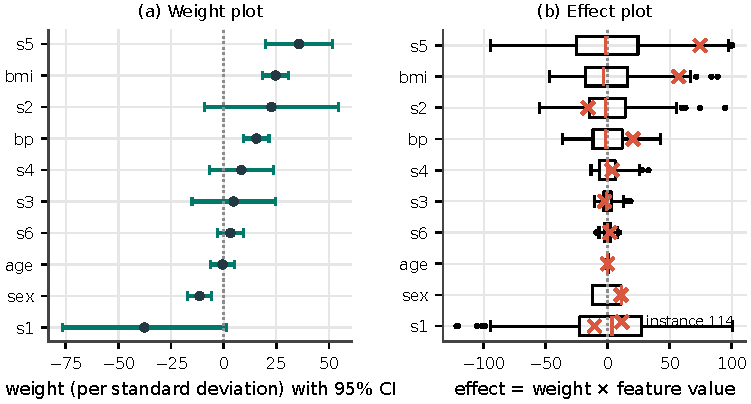
\includegraphics[width=\textwidth]{ch03/linear_weights}
\caption{A linear model of diabetes progression with standardised features. (a) Weights with
95\% confidence intervals. (b) Distribution of the effects of each feature; the crosses are the
effects for the instance with the highest prediction.}
\label{fig:linear}
\end{figure}

Do linear models produce good explanations? They are contrastive, but the reference is an instance
with all features at zero, which is meaningless unless the features are centred; they are
selective only if they are sparse (for instance, fitted with a Lasso penalty); and they are exactly faithful\index{faithfulness} to
the linear model, while the scientific or causal validity of their interpretation depends on whether the
relationship really is linear. Their great advantages are simplicity and
generality. Their disadvantages: every non-linearity or interaction must be hand-crafted, their
predictive performance is often not the best, and the interpretation of a weight depends on all
the other features in the model, which can make it counter-intuitive.

\subsection{Logistic regression}

A linear model is not appropriate for classification: it does not output probabilities, it
extrapolates below zero and above one, and it does not extend to more than two classes.
\emph{Logistic regression\index{logistic regression|textbf}} models the probability of the positive class as
\begin{equation}
  P(y=1\mid x)=\frac{1}{1+e^{-(\beta_0+\beta_1x_1+\dots+\beta_px_p)}},
\end{equation}
so the weights no longer act linearly on the probability. Rearranging, we find a linear model for
the \emph{log odds},
\begin{equation}
  \ln\frac{P(y=1\mid x)}{1-P(y=1\mid x)}=\beta_0+\beta_1x_1+\dots+\beta_px_p,
\end{equation}
and increasing $x_j$ by one unit multiplies the \emph{odds} by $e^{\beta_j}$, the \emph{odds
ratio\index{odds ratio|textbf}}. The templates become: for a numerical feature, an increase of one unit changes the odds by
a factor $e^{\beta_j}$, all the other features staying the same; for a binary feature, changing from
the reference level multiplies the odds by $e^{\beta_j}$; the intercept gives the odds $e^{\beta_0}$
of a reference instance.

\begin{pylisting}[label={lst:loans}]{Synthetic loan applications used in several examples}
"""Synthetic loan applications used in the interpretability examples (Unit 3)."""
import numpy as np

FEATURES = ["income", "debt_ratio", "years_job", "prev_default"]

def loan_data(n=5000, seed=3):
    rng = np.random.default_rng(seed)
    income = rng.normal(30, 8, n)                       # thousand EUR per year
    debt = rng.uniform(0, 0.8, n)                       # debt-to-income ratio
    years = rng.integers(0, 30, n).astype(float)        # years in the current job
    prev = (rng.random(n) < 0.15).astype(float)         # previous default (0/1)
    logit = -2 + 0.08 * income - 3 * debt + 0.03 * years - 1.2 * prev
    y = (rng.random(n) < 1 / (1 + np.exp(-logit))).astype(int)     # 1 = repays
    return np.c_[income, debt, years, prev], y
\end{pylisting}

\Cref{lst:odds} fits a logistic regression to the synthetic loan data of \cref{lst:loans}. Each
additional thousand euros of income multiplies the odds of repaying by 1.081 (an 8\% increase);
an increase of the debt ratio by 0.1 multiplies them by $e^{-0.2976}=0.74$; a previous default
divides them by almost three (0.369). For an applicant with a probability of repaying of 0.30,
10,000 more euros of income would raise it to 0.48. As always, these are statements about the
model, and correlation does not imply causation.

\begin{pylisting}[label={lst:odds}]{Odds ratios of a logistic regression}
import numpy as np
from sklearn.linear_model import LogisticRegression
from loans import FEATURES, loan_data

X, y = loan_data()
m = LogisticRegression(C=1e6, max_iter=5000).fit(X, y)      # practically unregularised
for name, b in zip(FEATURES, m.coef_[0]):
    print(f"{name:13s} beta={b:7.3f}   odds ratio exp(beta)={np.exp(b):6.3f}")
odds = 0.3 / 0.7 * np.exp(10 * m.coef_[0][0])               # P(repay)=0.3, +10k EUR income
p_new = odds / (1 + odds)
print(f"an applicant with P(repay)=0.30 earning 10k EUR more: P(repay)={p_new:.2f}")
\end{pylisting}
\begin{pyoutput}
income        beta=  0.078   odds ratio exp(beta)= 1.081
debt_ratio    beta= -2.976   odds ratio exp(beta)= 0.051
years_job     beta=  0.031   odds ratio exp(beta)= 1.032
prev_default  beta= -0.998   odds ratio exp(beta)= 0.369
an applicant with P(repay)=0.30 earning 10k EUR more: P(repay)=0.48
\end{pyoutput}

\subsection{Decision trees}

Linear and logistic models fail when the relationship between features and target is non-linear or
when features interact. Decision trees\index{decision tree}, such as CART \citep{breiman1984classification}, split the data
recursively, choosing at each node the feature and cut-off that best separate the target (minimum
impurity), until a stopping criterion is reached. The interpretation is simple: starting from the
root, each edge selects a subset of the data, and the leaf gives the prediction; all the conditions
on the path are connected by ``and'':
\begin{center}
\textsc{if} feature $x$ is smaller (or bigger) than threshold $c$ \textsc{and} \dots\ \textsc{then}
the predicted outcome is $\hat y_{\text{leaf}}$.
\end{center}
Trees capture interactions naturally, have a natural visualisation, and produce good explanations:
contrastive (``if the feature had been above the threshold, the prediction would have been\dots''),
selective if the tree is short, and simple. Their drawbacks are that linear relationships are
approximated by steps (lack of smoothness), and that trees are \emph{unstable}: small changes in the
training data can produce a completely different tree (\cref{sec:ensembles}), which does not inspire
confidence in their interpretation.

\subsection{Decision rules}

A \emph{decision rule\index{decision rules|textbf}} is an \textsc{if-then} statement with a condition (antecedent) and a
prediction. Decision rules are probably the most interpretable prediction models, provided the
conditions use intelligible features, are short, and there are not too many rules. The usefulness of
a rule is summarised by its \emph{support} or \emph{coverage\index{coverage|textbf}}, the fraction of instances to which its
condition applies, and its \emph{accuracy\index{accuracy|textbf}} or \emph{confidence}, the fraction of those it predicts
correctly (\cref{sec:unsupervised}). Rules can be combined in a \emph{decision list}, which orders
them (the first rule that applies decides), or in a \emph{decision set}, a democracy of rules in
which some may have more voting\index{voting} power; interpretability suffers when several rules of a set apply.

Some algorithms that learn rules are:
\begin{itemize}
  \item \emph{OneR\index{OneR|textbf}} \citep{holte1993very}, which learns rules from a single feature: for each
        feature (discretised if needed) it predicts the majority class of each value, and keeps the
        feature with the lowest error. It is a useful baseline;
  \item \emph{sequential covering}, which learns one rule at a time and removes the examples it
        covers, as in RIPPER \citep{cohen1995fast};
  \item \emph{Bayesian rule lists} \citep{letham2015interpretable}, which combine pre-mined frequent
        patterns into a decision list using Bayesian statistics.
\end{itemize}

\begin{pylisting}[label={lst:oner}]{The OneR algorithm on the loan data}
import numpy as np
from loans import FEATURES, loan_data

def one_r(Xcat, y):
    """OneR (Holte, 1993): the best set of rules that uses a single feature."""
    best = None
    for j in range(Xcat.shape[1]):
        rule = {v: np.bincount(y[Xcat[:, j] == v], minlength=2).argmax()   # majority class
                for v in np.unique(Xcat[:, j])}
        acc = np.mean([rule[v] == t for v, t in zip(Xcat[:, j], y)])
        if best is None or acc > best[1]:
            best = (j, acc, rule)
    return best

X, y = loan_data()
cuts = [np.quantile(X[:, j], [0.25, 0.5, 0.75]) for j in range(3)]    # quartiles
Xcat = np.c_[np.column_stack([np.digitize(X[:, j], cuts[j]) for j in range(3)]), X[:, 3]]
j, acc, rule = one_r(Xcat, y)
base = max(y.mean(), 1 - y.mean())
print(f"OneR uses '{FEATURES[j]}': accuracy {acc:.3f} "
      f"(predicting the majority: {base:.3f})")
for v, c in rule.items():
    outcome = "repays" if c else "defaults"
    print(f"  IF {FEATURES[j]} is in quartile {int(v) + 1} THEN {outcome}")
\end{pylisting}
\begin{pyoutput}
OneR uses 'debt_ratio': accuracy 0.653 (predicting the majority: 0.619)
  IF debt_ratio is in quartile 1 THEN repays
  IF debt_ratio is in quartile 2 THEN defaults
  IF debt_ratio is in quartile 3 THEN defaults
  IF debt_ratio is in quartile 4 THEN defaults
\end{pyoutput}

In \cref{lst:oner}, OneR chooses the debt ratio: applicants in the lowest quartile repay, the rest
default. The single rule reaches an accuracy of 0.653, only a few points above always predicting
the majority class (0.619), a reminder that simple rules are good baselines but rarely good models.
Rules are easy to interpret, as expressive as trees while often more compact, fast at prediction
time, robust to monotone transformations of the features, and sparse. On the other hand, most rule
learners focus on classification, need discretised features, and describe linear relationships
poorly.

\subsection{RuleFit}

\emph{RuleFit\index{RuleFit|textbf}} \citep{friedman2008predictive} combines the strengths of rules and linear models. It
grows trees to predict the outcome, turns every path from the root to a node into a decision rule\index{decision rules}
(discarding the node predictions), and fits a sparse (Lasso) linear model that uses the original
features together with the rules as binary features. The rules capture interactions automatically.
The interpretation is that of a linear model: if all the conditions of rule $r_k$ apply, the
prediction changes by $\alpha_k$ (in classification, the odds are multiplied by $e^{\alpha_k}$). For
one instance only a handful of rules usually matter, and RuleFit comes with useful diagnostics,
such as feature importances\index{feature importance} and partial dependence\index{partial dependence plot} plots. Its drawbacks: it sometimes keeps many
rules with non-zero weights, and the ``all other features fixed'' interpretation becomes problematic
when rules overlap.

\subsection{Other interpretable models}

\emph{Naive Bayes} makes clear how much each feature value contributes towards each class, because
under the independence assumption the log-odds are a sum of per-feature terms. \emph{$k$-nearest
neighbours\index{k-nearest neighbours@$k$-nearest neighbours|textbf}} has no global or modular interpretation, but each prediction can be explained by
showing the $k$ neighbours, which works if the instances are themselves understandable (it is the
basis of the example-based explanations of \cref{sec:examplebased}). \emph{Generalised additive
models} learn a flexible function of each feature and add them, keeping the model readable feature
by feature \citep{lou2012intelligible}. \citet{rudin2019stop} argues that for high-stakes decisions we
should use such interpretable models instead of explaining black boxes, since in many problems they
are as accurate.

% ---------------------------------------------------------------------
\section{Model-agnostic methods}\label{sec:agnostic}

Separating the explanations from the model gives flexibility: the same method can explain, and
compare, any model. A good model-agnostic explanation system has \emph{model flexibility} (it is not
tied to a class of models), \emph{explanation flexibility} (it is not tied to a form of explanation)
and \emph{representation flexibility} (it can use features different from those of the model)
\citep{ribeiro2016model}. \Cref{fig:layers} places these methods in context: the world is digitised
into data, a black-box model is fitted to the data, interpretability methods sit on top of the model,
and a human receives their output. Statisticians, concerned with data collection and inference, tend
to skip the black-box layer and work directly with interpretable models; machine learning
practitioners tend to skip the interpretability layer and use the predictions directly.

\begin{figure}[htbp]
\centering
\begin{tikzpicture}[font=\small\sffamily,
  l/.style={draw=edmnavy,fill=edmnavy!6,rounded corners=2pt,minimum width=62mm,minimum height=7mm},
  arr/.style={-{Stealth[length=2mm]},edmnavy,thick}]
  \node[l] (w) at (0,0) {world};
  \node[l] (d) at (0,1.1) {data};
  \node[l] (b) at (0,2.2) {black-box model};
  \node[l,fill=edmbronze!25,draw=edmbronze] (i) at (0,3.3) {interpretability methods};
  \node[l] (h) at (0,4.4) {human};
  \foreach \a/\b in {w/d,d/b,b/i,i/h} \draw[arr] (\a) -- (\b);
  \node[anchor=west,font=\scriptsize\sffamily,align=left] at (3.4,0.55) {measurement};
  \node[anchor=west,font=\scriptsize\sffamily,align=left] at (3.4,1.65) {learning};
  \node[anchor=west,font=\scriptsize\sffamily,align=left] at (3.4,2.75) {explanation};
  \node[anchor=west,font=\scriptsize\sffamily,align=left] at (3.4,3.85) {communication};
\end{tikzpicture}
\caption{The layers of interpretability: model-agnostic methods sit between the model and the
human.}
\label{fig:layers}
\end{figure}

To illustrate the methods we use a problem whose true structure is known, the Friedman regression
function \citep{friedman1991multivariate}: ten features uniformly distributed in $[0,1]$, of which
only the first five matter,
\begin{equation}\label{eq:friedman}
  y=10\sin(\pi x_1x_2)+20(x_3-0.5)^2+10x_4+5x_5+\varepsilon .
\end{equation}
The effect of $x_3$ is quadratic, those of $x_4$ and $x_5$ linear, $x_1$ and $x_2$ interact, and
$x_6,\dots,x_{10}$ are pure noise. We fit a gradient boosting\index{gradient boosting}\index{boosting} model to 1400 examples and pretend that
we do not know the function.

\subsection{Partial dependence plots}

The \emph{partial dependence\index{partial dependence plot|textbf} plot} (PDP) shows the marginal effect of one or two features on the
prediction of a model \citep{friedman2001greedy}. If $x_S$ are the features of interest and $x_C$ the
others, the partial dependence function averages the model over the distribution of $x_C$,
\begin{equation}
  \hat f_S(x_S)=\E_{x_C}\bigl[\hat f(x_S,x_C)\bigr]\approx\frac1n\sum_{i=1}^{n}\hat f\bigl(x_S,x_C^{(i)}\bigr):
\end{equation}
for each value of $x_S$ on a grid, we replace the feature in every instance by that value, predict,
and average. In classification, it shows the probability of a class. The PDP shows whether the
relationship between a feature and the prediction is linear, monotone or more complex, and it has a
causal interpretation \emph{for the model} (we intervene on a feature and observe the prediction),
though not necessarily for the world.

\Cref{fig:pdpice}a recovers the structure of \cref{eq:friedman}: a parabola for $x_3$, a straight line
for $x_4$ and a flat line for the noise feature $x_6$. In \cref{lst:pdph} the partial dependence of
$x_4$ grows from 9.77 at 0 to 19.00 at 1, a slope of about 9.2 against the true 10.

\begin{figure}[htbp]
\centering
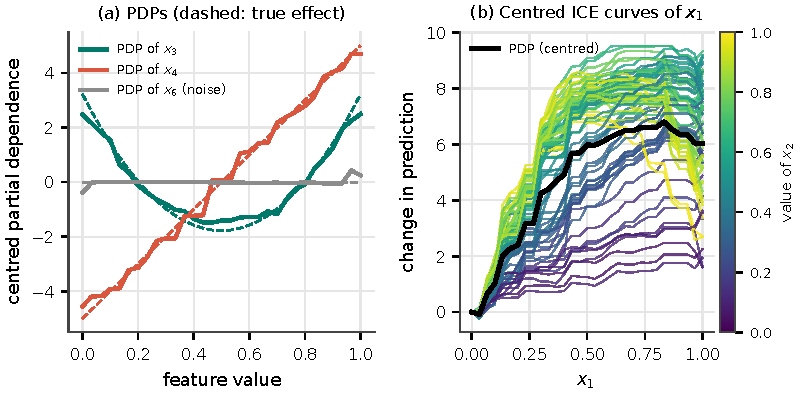
\includegraphics[width=\textwidth]{ch03/pdp_ice}
\caption{(a) Partial dependence plots of three features of a gradient boosting model of the
Friedman function, with the true effects dashed. (b) Centred ICE curves of $x_1$ for 80 instances,
coloured by their value of $x_2$; the thick line is the centred PDP.}
\label{fig:pdpice}
\end{figure}

PDPs are intuitive and easy to implement. Their main limitation is the assumption that the features
in $x_S$ are independent of those in $x_C$: if they are correlated, the average includes combinations
that are unlikely or impossible (a person 2 metres tall weighing 50 kg). Accumulated local effects\index{accumulated local effects}
(ALE) plots address this problem by averaging over the conditional distribution in small intervals
\citep{apley2020visualizing}. PDPs can display at most two features at once, should show the
distribution of the feature (they are unreliable where there are few data), and can hide
heterogeneous effects: if a feature increases the prediction for half of the data and decreases it
for the other half, the PDP is a flat line.

\subsection{Individual conditional expectation}

\emph{Individual conditional expectation\index{individual conditional expectation|textbf}} (ICE) plots draw one line per instance, showing how its
prediction changes when the feature changes and everything else stays fixed \citep{goldstein2015peeking};
the PDP is the average of the ICE lines. ICE plots reveal heterogeneous effects and interactions.
Because the lines start at different heights, it is useful to \emph{centre} them at a reference value
of the feature (for instance, its minimum) and plot only the change in prediction.
\Cref{fig:pdpice}b shows centred ICE curves of $x_1$: their slopes depend strongly on $x_2$ (yellow
lines, with high $x_2$, rise much more), which reveals the interaction $\sin(\pi x_1x_2)$ hidden in the
average. ICE plots are even more intuitive than PDPs, but they can display only one feature, become
overcrowded (use transparency or a sample of lines), and share the problem of unrealistic points with
correlated features.

\subsection{Feature interaction}

Two features \emph{interact} when the effect of one depends on the value of the other, that is, when
the prediction is not the sum of their individual effects. For instance, a model of house prices
without interaction might add 100,000 euros for a big house and 50,000 for a good location to a base
of 150,000; with an interaction, a big house in a good location would be worth an extra amount on top
of those two effects. Friedman's \emph{H-statistic\index{H-statistic@$H$-statistic|textbf}} \citep{friedman2008predictive} measures the share of
the variance of the joint partial dependence\index{partial dependence plot} that is due to the interaction. If two features $x_j$
and $x_k$ do not interact, their (centred) partial dependence decomposes as
$PD_{jk}(x_j,x_k)=PD_j(x_j)+PD_k(x_k)$, and
\begin{equation}
  H^2_{jk}=\frac{\sum_{i=1}^{n}\bigl[PD_{jk}(x_j^{(i)},x_k^{(i)})-PD_j(x_j^{(i)})-PD_k(x_k^{(i)})\bigr]^2}
                {\sum_{i=1}^{n}PD_{jk}^2(x_j^{(i)},x_k^{(i)})}.
\end{equation}
Similarly, the interaction of $x_j$ with all the other features compares the prediction with
$PD_j(x_j)+PD_{-j}(x_{-j})$. The statistic is dimensionless and, under an orthogonal decomposition (for instance with independent
features), a fraction between 0 (no interaction) and 1 (the
effect is pure interaction), and has a theory behind it, but it is expensive to compute (the cost
grows with the square of the number of instances, which is why it is estimated on a sample, adding
variance to the estimate), it is unclear when an interaction is significantly larger than zero, and it
does not show the shape of the interaction (a two-feature PDP does). With dependent features or estimated partial dependences it can exceed 1, and it is
undefined when the denominator vanishes, so the sampling scheme and the support of the data must be
checked before interpreting it. \Cref{lst:pdph} and
\cref{fig:importanceh}b find the only interaction of \cref{eq:friedman}: $H^2_{12}=0.083$, while the other
pairs are around 0.002.

\begin{pylisting}[label={lst:pdph}]{Partial dependence and Friedman's H statistic computed from scratch}
import numpy as np
from sklearn.datasets import make_friedman1
from sklearn.ensemble import GradientBoostingRegressor
from sklearn.model_selection import train_test_split

X, y = make_friedman1(n_samples=2000, n_features=10, noise=1.0, random_state=0)
X_tr, X_te, y_tr, y_te = train_test_split(X, y, test_size=0.3, random_state=0)
model = GradientBoostingRegressor(n_estimators=400, max_depth=3, learning_rate=0.05,
                                  random_state=0).fit(X_tr, y_tr)

def pd_at(X, cols, values):
    """Partial dependence: average prediction with the columns `cols` set to `values`."""
    Xv = X.copy()
    Xv[:, cols] = values
    return model.predict(Xv).mean()

def h2(X, j, k):
    """Friedman's H^2 for features j and k, from centred partial dependence functions."""
    pd = lambda cols: np.array([pd_at(X, cols, x[cols]) for x in X])
    pj, pk, pjk = pd([j]), pd([k]), pd([j, k])
    pj, pk, pjk = pj - pj.mean(), pk - pk.mean(), pjk - pjk.mean()
    return np.sum((pjk - pj - pk) ** 2) / np.sum(pjk ** 2)

S = X_te[:120]
print("PD of x4 at 0, 0.5, 1:", " ".join(f"{pd_at(S, [3], v):.2f}" for v in (0, 0.5, 1)))
for j, k in [(0, 1), (0, 3), (3, 4)]:
    print(f"H^2(x{j + 1}, x{k + 1}) = {h2(S, j, k):.3f}")
\end{pylisting}
\begin{pyoutput}
PD of x4 at 0, 0.5, 1: 9.77 14.44 19.00
H^2(x1, x2) = 0.083
H^2(x1, x4) = 0.002
H^2(x4, x5) = 0.002
\end{pyoutput}

\subsection{Permutation feature importance}

The importance of a feature can be measured by the increase of the prediction error of the model
after \emph{permuting} the values of that feature, which breaks its relationship with the target
\citep{breiman2001random,fisher2019all}: a feature is important if the model relied on it. The
algorithm is:
\begin{enumerate}
  \item compute the error $e_{\text{orig}}$ of the trained model (for example, the MSE\index{mean squared error (MSE)} or $1-\mathrm{AUC}$);
  \item for each feature $j$, permute its column in the data, compute the error $e_{\text{perm},j}$,
        and define the importance as the ratio $e_{\text{perm},j}/e_{\text{orig}}$ or the difference
        $e_{\text{perm},j}-e_{\text{orig}}$ (repeating the permutation to reduce the variance);
  \item sort the features by importance.
\end{enumerate}
Its interpretation is clear (the loss of performance when the information of the feature is
destroyed), it gives a compressed global view of the model, and the ratio version is comparable
across problems. It needs the true target (it cannot be computed with only a model and unlabelled
data), it is tied to the error of the model, which is not what we want if the question is how much of
the output varies with each feature, and it should be computed on \emph{test} data, since importance
on training data reflects what the model memorised. With correlated features, permuting one creates
unrealistic instances and the importance is shared between the correlated features.

\begin{pylisting}[label={lst:importance}]{Permutation importance, impurity importance and global surrogates}
import numpy as np
from sklearn.datasets import make_friedman1
from sklearn.ensemble import RandomForestRegressor
from sklearn.inspection import permutation_importance
from sklearn.metrics import r2_score
from sklearn.model_selection import train_test_split
from sklearn.tree import DecisionTreeRegressor

X, y = make_friedman1(n_samples=2000, n_features=10, noise=1.0, random_state=0)
X_tr, X_te, y_tr, y_te = train_test_split(X, y, test_size=0.3, random_state=0)
rf = RandomForestRegressor(300, random_state=0).fit(X_tr, y_tr)
pi = permutation_importance(rf, X_te, y_te, n_repeats=10, random_state=0)   # drop in R^2
for j in np.argsort(-pi.importances_mean)[:6]:
    print(f"x{j + 1:<2d} permutation={pi.importances_mean[j]:.3f} "
          f"+/- {pi.importances_std[j]:.3f}   impurity={rf.feature_importances_[j]:.3f}")
for depth in (2, 3, 5):        # global surrogate: a small tree that imitates the forest
    tree = DecisionTreeRegressor(max_depth=depth, random_state=0)
    tree.fit(X_tr, rf.predict(X_tr))
    print(f"surrogate tree of depth {depth}: R^2 with respect to the forest = "
          f"{r2_score(rf.predict(X_te), tree.predict(X_te)):.3f}")
\end{pylisting}
\begin{pyoutput}
x4  permutation=0.714 +/- 0.032   impurity=0.367
x1  permutation=0.437 +/- 0.021   impurity=0.208
x2  permutation=0.386 +/- 0.036   impurity=0.216
x5  permutation=0.138 +/- 0.012   impurity=0.097
x3  permutation=0.077 +/- 0.005   impurity=0.057
x7  permutation=0.000 +/- 0.000   impurity=0.012
surrogate tree of depth 2: R^2 with respect to the forest = 0.510
surrogate tree of depth 3: R^2 with respect to the forest = 0.747
surrogate tree of depth 5: R^2 with respect to the forest = 0.877
\end{pyoutput}

\Cref{lst:importance} and \cref{fig:importanceh}a compare permutation importance\index{feature importance!permutation} on test data with the
impurity-based\index{feature importance} importance of a random forest (\cref{sec:enspractice}). Both rank $x_4$, $x_1$, $x_2$,
$x_5$ and $x_3$ first, but the impurity importance gives every noise feature around 0.01, whereas their
permutation importance is zero: the forest used them to fit noise in the training data, and that does
not help on new data.

\begin{figure}[htbp]
\centering
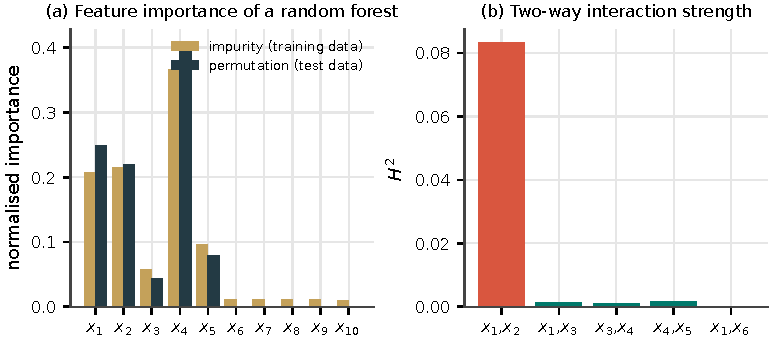
\includegraphics[width=\textwidth]{ch03/importance_h}
\caption{(a) Normalised impurity-based and permutation importance of a random forest fitted to the
Friedman function ($x_6$ to $x_{10}$ are noise). (b) $H^2$ interaction strength for five pairs of
features of the gradient boosting model.}
\label{fig:importanceh}
\end{figure}

\subsection{Global surrogate models}

A \emph{global surrogate\index{global surrogate|textbf}} is an interpretable model trained to approximate the predictions of a
black box; it is the mimetic\index{mimetic classifier} classifier of \cref{sec:drawbacks}, under another name (it is also known
as approximation model, metamodel, response surface model or emulator). The procedure is to choose a
data set, obtain the predictions $\hat y$ of the black box on it, train an interpretable model
(linear, tree\dots) on those predictions, and measure how well it replicates them, for instance with
\begin{equation}
  R^2=1-\frac{\sum_i(\hat y_*^{(i)}-\hat y^{(i)})^2}{\sum_i(\hat y^{(i)}-\bar{\hat y})^2},
\end{equation}
where $\hat y_*$ are the predictions of the surrogate. Only then is the surrogate interpreted. In
\cref{lst:importance}, a tree of depth 2 captures 51\% of the variance of the forest's predictions,
depth 3 captures 75\% and depth 5 captures 88\%.

The method is flexible, intuitive, and its fidelity\index{fidelity} is easy to measure, but several cautions apply.
It draws conclusions about the model, not about the data. There is no clear cut-off for a good
enough $R^2$, and the surrogate may be very close to the black box in some regions and far from it in
others. If the input distribution is changed, for instance by weighting the instances around a
particular point, the surrogate becomes \emph{local}, which leads to LIME\index{LIME}.

\subsection{Local surrogates: LIME}

LIME\index{LIME} (local interpretable model-agnostic explanations, \citealp{ribeiro2016should}) was introduced in
\cref{sec:drawbacks}. To explain the prediction of a black box $f$ for an instance $x$, it
\begin{enumerate}
  \item generates a data set of perturbed instances and obtains the black box predictions for them;
  \item weights the new samples by their proximity to $x$, with a kernel $\pi_x$;
  \item fits a weighted interpretable model (a Lasso, a short tree) with a small number $K$ of features;
  \item explains the prediction by interpreting the local model.
\end{enumerate}
The local model must be faithful\index{faithfulness} in the neighbourhood of $x$ (\emph{local fidelity\index{fidelity|textbf}}), not globally.
How the perturbations are generated depends on the data: for text, LIME removes words at random and
represents each variant by the presence or absence of each word; for images, it switches off
\emph{superpixels} (groups of similar neighbouring pixels), replacing them by grey; for tabular data,
it draws each feature from a normal distribution with the mean and standard deviation of the training
data, so the samples come from the centre of the data and not from around $x$, and the kernel decides
which of them matter.

\begin{pylisting}[label={lst:lime}]{A minimal implementation of LIME for tabular data}
import numpy as np
from sklearn.ensemble import GradientBoostingRegressor
from sklearn.linear_model import Ridge
from apartments import FEATURES, apartments

def lime(f, X_train, x, n=5000, kernel_width=None, seed=0):
    """LIME for tabular data: a weighted linear model fitted to perturbed samples."""
    rng = np.random.default_rng(seed)
    mu, sd = X_train.mean(axis=0), X_train.std(axis=0)
    # samples from the data distribution
    Z = rng.normal(mu, sd, (n, len(x)))
    d = np.linalg.norm((Z - x) / sd, axis=1)              # standardised distance to x
    width = kernel_width or 0.75 * np.sqrt(len(x))
    w = np.exp(-d ** 2 / width ** 2)                      # proximity weights
    g = Ridge(alpha=1.0).fit((Z - mu) / sd, f(Z), sample_weight=w)
    return g.coef_, g.score((Z - mu) / sd, f(Z), sample_weight=w)

X, y = apartments()
model = GradientBoostingRegressor(random_state=0).fit(X, y)
x = np.array([1.0, 0.0, 50.0, 2.0])         # park nearby, cat forbidden, 50 m2, 2nd floor
for seed, width in [(0, None), (1, None), (2, None), (0, 0.5)]:
    coef, fid = lime(model.predict, X, x, kernel_width=width, seed=seed)
    print(f"seed {seed}, width {width or 1.5:.1f}: "
          + " ".join(f"{n}={c:.1f}" for n, c in zip(FEATURES, coef)) + f"  R2={fid:.2f}")
\end{pylisting}
\begin{pyoutput}
seed 0, width 1.5: park_nearby=8.8 cat_allowed=6.4 area_m2=71.3 floor=6.3  R2=0.97
seed 1, width 1.5: park_nearby=9.0 cat_allowed=6.4 area_m2=70.6 floor=5.6  R2=0.97
seed 2, width 1.5: park_nearby=8.7 cat_allowed=7.1 area_m2=71.4 floor=5.5  R2=0.97
seed 0, width 0.5: park_nearby=0.3 cat_allowed=0.7 area_m2=42.5 floor=-0.4  R2=0.80
\end{pyoutput}

\Cref{lst:lime} implements LIME and explains the price predicted by a gradient boosting\index{gradient boosting} model for a
flat of 50 square metres, on the second floor, near a park and in a building where cats are forbidden
(the synthetic apartment data of \cref{lst:apartments}). With the default kernel width the
explanation is stable across random seeds and faithful ($R^2=0.97$): the area dominates (71 thousand
euros per standard deviation), followed by the park (about 9). With a narrower kernel the explanation
changes completely (only the area matters, with half the weight) and is less faithful ($R^2=0.80$). Part of this change is not about locality: with unnormalised weights and a
fixed Ridge penalty, a narrower kernel also increases the relative regularisation, and the Gaussian
perturbations produce invalid inputs, such as fractional values of the binary features. A careful
implementation samples valid inputs, normalises the weights, reports the effective sample size\index{sample size}\index{effective sample size} and
measures fidelity on fresh perturbations.
This is LIME's main problem: the definition of the neighbourhood is an open question, there is no
principled way of choosing the kernel width, the Gaussian sampling ignores correlations between
features, and the explanations can be unstable \citep{alvarezmelis2018robustness}. They can also be
manipulated: a model can be built to behave in a biased way on real data and innocuously on the
perturbed samples that LIME generates \citep{slack2020fooling}. On the positive side, LIME works for
tabular data, text and images, its explanations are short and possibly contrastive, it gives a
fidelity measure, and it can use interpretable features different from those of the model.

\subsection{Shapley values}

The \emph{Shapley\index{Shapley values|textbf} value} comes from cooperative game theory \citep{shapley1953value}. It distributes the
payout of a game fairly among the players that cooperated to obtain it. To explain a prediction
\citep{strumbelj2014explaining}, the game is the prediction task for one instance, the players are its
feature values, and the payout is the prediction minus the average prediction. The value of a
coalition $S$ of features is the expected prediction when the features in $S$ are fixed to the values
of the instance and the others are drawn from the data,
$v(S)=\E\bigl[\hat f(x_S,X_{\bar S})\bigr]-\E[\hat f(X)]$, and the Shapley value of feature $j$ is its
average marginal contribution over all the coalitions:
\begin{equation}\label{eq:shapley}
  \phi_j=\sum_{S\subseteq F\setminus\{j\}}\frac{|S|!\,(p-|S|-1)!}{p!}\,\bigl(v(S\cup\{j\})-v(S)\bigr),
\end{equation}
where $F$ is the set of $p$ features. The weights correspond to averaging over all the orders in which
the features could join the coalition. The Shapley value is the only attribution that satisfies four
properties: \emph{efficiency} (the contributions add up to the difference between the prediction and
the average, $\sum_j\phi_j=\hat f(x)-\E[\hat f(X)]$), \emph{symmetry} (two features that contribute
equally to every coalition get the same value), \emph{dummy} (a feature that never changes the
prediction gets zero) and \emph{additivity} (for a sum of models, the values add).

\begin{pylisting}[label={lst:apartments}]{Synthetic apartment prices used in the explanation examples}
"""Synthetic apartment prices used in the explanation examples (Unit 3)."""
import numpy as np

FEATURES = ["park_nearby", "cat_allowed", "area_m2", "floor"]

def apartments(n=2000, seed=0):
    rng = np.random.default_rng(seed)
    area = rng.uniform(30, 120, n)
    park = (rng.random(n) < 0.5).astype(float)
    cat = (rng.random(n) < 0.6).astype(float)
    floor = rng.integers(0, 8, n).astype(float)
    price = (40 + 2.6 * area + 25 * park + 15 * cat + 3 * floor     # thousand EUR
             + 0.3 * park * (area - 75) + rng.normal(0, 12, n))
    return np.c_[park, cat, area, floor], price
\end{pylisting}

\begin{pylisting}[label={lst:shapley}]{Exact Shapley values by enumerating all coalitions}
from itertools import combinations
from math import factorial
import numpy as np
from sklearn.ensemble import GradientBoostingRegressor
from apartments import FEATURES, apartments

def shapley(f, x, background):
    """Exact Shapley values; absent features take their values from background data."""
    p = len(x)
    def value(S):                                   # v(S) = E[f(x_S, X_rest)]
        Z = background.copy()
        Z[:, list(S)] = x[list(S)]
        return f(Z).mean()
    phi = np.zeros(p)
    for j in range(p):
        others = [k for k in range(p) if k != j]
        for size in range(p):
            for S in combinations(others, size):
                weight = factorial(size) * factorial(p - size - 1) / factorial(p)
                phi[j] += weight * (value(S + (j,)) - value(S))
    return phi

X, y = apartments()
model = GradientBoostingRegressor(random_state=0).fit(X, y)
x = np.array([1.0, 0.0, 50.0, 2.0])
bg = X[np.random.default_rng(1).choice(len(X), 300, replace=False)]
phi = shapley(model.predict, x, bg)
base, pred = model.predict(bg).mean(), model.predict(x[None])[0]
for name, v in zip(FEATURES, phi):
    print(f"{name:12s} {v:+7.1f}")
print(f"average {base:.1f} + contributions {phi.sum():+.1f} = {base + phi.sum():.1f}"
      f"   (prediction {pred:.1f})")
\end{pylisting}
\begin{pyoutput}
park_nearby     +9.4
cat_allowed     -8.3
area_m2        -70.3
floor           -4.6
average 264.7 + contributions -73.9 = 190.8   (prediction 190.8)
\end{pyoutput}

\Cref{lst:shapley} computes the exact values for the flat explained with LIME\index{LIME}, enumerating the
$2^3$ coalitions of the other features for each of the four features and estimating $v(S)$ with 300
background flats. The average predicted price is 264.7 thousand euros and this flat's prediction is
190.8: being small (50 square metres) lowers the price by 70.3, the forbidden cats by 8.3 and the floor
by 4.6, while the park raises it by 9.4, and the contributions add up exactly to the difference of
$-73.9$ (\cref{fig:limeshap}a).

\begin{figure}[htbp]
\centering
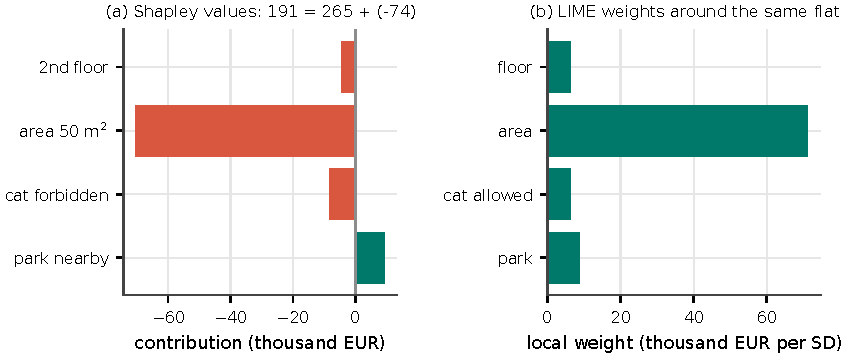
\includegraphics[width=\textwidth]{ch03/lime_shap}
\caption{Two explanations of the predicted price of one flat. (a) Shapley values: contributions to the
difference between the prediction and the average prediction. (b) LIME: weights of a local linear
model, per standard deviation of each feature.}
\label{fig:limeshap}
\end{figure}

Comparing the two panels of \cref{fig:limeshap} shows that the two methods answer different
questions. LIME's weights are local \emph{slopes}: around this flat, more area means a higher price
(+71 per standard deviation), and allowing cats would raise it. Shapley values are
\emph{contributions} relative to the average flat: this flat's area, smaller than average, lowers its
price by 70, and its cat ban lowers it by 8. Neither is ``the'' explanation.

For a fixed cooperative game, the Shapley value is the unique allocation that satisfies its classical
axioms (other attribution methods, such as integrated gradients\index{integrated gradients}, have axiomatic foundations of their
own \citep{sundararajan2017axiomatic}); it distributes the difference among the features according to
those axioms, and it allows contrastive explanations (against the average, or
against a subset of instances). But it is expensive: the number of coalitions grows exponentially with
the number of features, so in practice it is approximated by sampling coalitions and background
instances \citep{strumbelj2014explaining} or computed with model-specific algorithms, as in the SHAP\index{SHAP}
library \citep{lundberg2017unified}. It is also easy to misinterpret: the Shapley value of a feature is
\emph{not} the difference in prediction if the feature were removed from the model, and it does not
support statements such as ``if I earned 300 euros more, my score would go up by 5 points'', because it
returns one value per feature, not a model. It uses all the features, so it is the wrong method if
sparse explanations are wanted, and, like the PDP, it evaluates the model on unrealistic combinations
when features are correlated.

% ---------------------------------------------------------------------
\section{Example-based explanations}\label{sec:examplebased}

Example-based methods explain a model, or the data it was trained on, by selecting particular
instances instead of summarising features. People reason this way all the time: a physician who
sees a patient with an unusual cough remembers a similar case; a data scientist starting a project
reuses the code of a similar one; a firefighter decides not to enter a burning house because a
similar one collapsed. These methods are mostly model-agnostic, but they only make sense if an
instance can be presented in a way people understand, as with images or text; they work poorly for
tabular data with hundreds of features. We consider four kinds: counterfactual instances, adversarial
examples\index{adversarial example}, prototypes\index{prototypes and criticisms} and criticisms, and influential instances\index{influential instance} ($k$-nearest neighbours\index{k-nearest neighbours@$k$-nearest neighbours}, the fifth,
was discussed in \cref{sec:intmodels}).

\subsection{Counterfactual explanations}

A counterfactual explanation\index{counterfactual explanation} describes a causal situation of the form ``if $X$ had not occurred, $Y$
would not have occurred''. For a prediction, the ``event'' is the predicted outcome and the ``causes''
are the feature values of the instance: even if the relation between inputs and outcome is not causal
in the world, it is causal \emph{for the model}. A counterfactual explanation of a prediction
describes \emph{the smallest change to the feature values that changes the prediction to a
predefined output}. Peter applies for a loan and is rejected: what is the smallest change to his
income or debts that would get him the loan? Anna's model predicts that her flat can be rented for
900 euros, but she expected 1000: what would make it worth 1000?

Counterfactuals are human-friendly explanations: they are contrastive and selective. A good
counterfactual should produce the desired prediction as closely as possible, be as similar as possible
to the instance, change as few features as possible, and have likely feature values (we cannot suggest
a flat with a negative size). It should also be \emph{actionable}: changing one's age or past is not
possible, and recommending it is useless \citep{ustun2019actionable}. There are usually many
counterfactuals (a \emph{Rashomon} effect), which can be addressed by reporting several diverse ones
\citep{mothilal2020explaining} or by a criterion to choose the best.

\citet{wachter2018counterfactual} proposed to find a counterfactual $x'$ for the instance $x$ and the
desired outcome $y'$ by minimising
\begin{equation}
  L(x,x',y',\lambda)=\lambda\,\bigl(\hat f(x')-y'\bigr)^2+d(x,x'),
\end{equation}
where the first term pushes the prediction towards $y'$ and the second keeps $x'$ close to $x$, with the
Manhattan distance weighted by the inverse \emph{median absolute deviation} of each feature,
\begin{equation}
  d(x,x')=\sum_{j=1}^{p}\frac{|x_j-x'_j|}{\mathrm{MAD}_j},\qquad
  \mathrm{MAD}_j=\operatorname{median}_{i}\bigl|x_{ij}-\operatorname{median}_l x_{lj}\bigr| .
\end{equation}
This distance is robust to outliers and, being an $L_1$ distance, prefers changing few features. The
algorithm starts with a small $\lambda$ and increases it until the prediction of the minimiser is
within a tolerance $\epsilon$ of $y'$, so that among the solutions that achieve the outcome it returns a
close one. The method needs no access to the data or to the internals of the model, works even for
systems that do not use machine learning, and is easy to implement; but there is no guarantee of
finding a counterfactual within the tolerance, and categorical features with many levels make the search
expensive.

\begin{pylisting}[label={lst:counterfactual}]{A counterfactual explanation with the method of Wachter et al.}
import numpy as np
from scipy.optimize import minimize
from sklearn.linear_model import LogisticRegression
from loans import FEATURES, loan_data

X, y = loan_data()
model = LogisticRegression(C=1e6, max_iter=5000).fit(X, y)
f = lambda Z: model.predict_proba(Z)[:, 1]                    # P(repay)
mad = np.median(np.abs(X - np.median(X, axis=0)), axis=0)      # median absolute deviation
lo, hi = X.min(axis=0), X.max(axis=0)                          # plausible ranges

def counterfactual(x, target=0.5, free=(0, 1), lambdas=(1, 10, 100, 1000, 10000), tol=0.01):
    """Wachter et al.: minimise lam*(f(x')-target)^2 + MAD-weighted L1 distance to x."""
    free = list(free)
    def loss(z, lam):
        xc = x.copy()
        xc[free] = z
        out = np.sum(np.maximum(lo - xc, 0) + np.maximum(xc - hi, 0))   # stay plausible
        dist = np.sum(np.abs(xc - x)[free] / mad[free])          # MAD-weighted L1 distance
        return lam * (f(xc[None])[0] - target) ** 2 + dist + 1e3 * out
    z = x[free].copy()
    for lam in lambdas:                                        # raise lambda until close
        z = minimize(loss, z, args=(lam,), method="Nelder-Mead").x
        xc = x.copy()
        xc[free] = z
        if abs(f(xc[None])[0] - target) <= tol:
            break
    return xc

peter = np.array([30.0, 0.45, 5.0, 0.0])     # income, debt ratio, years in job, no default
# only income and debt ratio may change; aim just above the bank's threshold of 0.5
cf = counterfactual(peter, target=0.51, tol=0.005)
print(f"Peter:          P(repay) = {f(peter[None])[0]:.3f}")
print(f"counterfactual: P(repay) = {f(cf[None])[0]:.3f}")
print("decision:", "approved" if f(cf[None])[0] >= 0.5 else "still rejected")
for name, a, b in zip(FEATURES, peter, cf):
    if abs(a - b) > 1e-3:
        print(f"  {name}: {a:.3f} -> {b:.3f}")
\end{pylisting}
\begin{pyoutput}
Peter:          P(repay) = 0.289
counterfactual: P(repay) = 0.507
decision: approved
  debt_ratio: 0.450 -> 0.139
\end{pyoutput}

\Cref{lst:counterfactual} and \cref{fig:counterfactual} find a counterfactual for Peter with the
logistic regression of \cref{lst:odds}, allowing only his income and debt ratio to change and keeping
them within the range of the data. His probability of repaying is 0.289; reducing his debt ratio from
0.45 to 0.14 raises it to 0.507, just above the bank's threshold of 0.5. The search aims slightly above
the threshold and the listing checks the decision: a counterfactual is valid only if it obtains the
desired decision, and accepting any point within a tolerance on either side of 0.5 could leave Peter
still rejected. The $L_1$ distance produced a sparse answer: it
was cheaper, in units of median absolute deviation, to reduce the debt than to increase the income.

\begin{figure}[htbp]
\centering
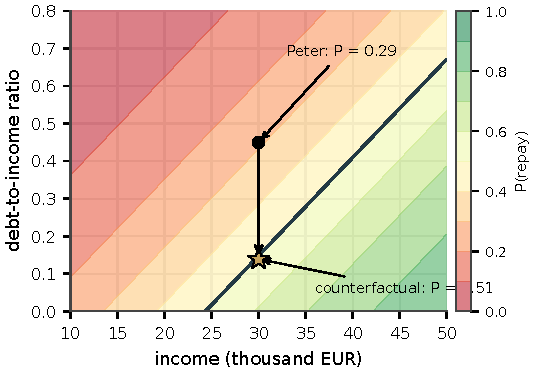
\includegraphics[width=0.66\textwidth]{ch03/counterfactual}
\caption{A counterfactual explanation for a rejected loan application. The colours show the predicted
probability of repayment as a function of income and debt ratio (other features fixed); the line is the
acceptance boundary.}
\label{fig:counterfactual}
\end{figure}

\subsection{Adversarial examples}

An \emph{adversarial example\index{adversarial example|textbf}} is an instance with small, intentional perturbations that make a model
give a false prediction: a counterfactual whose aim is to deceive the model rather than to explain it.
A stop sign with a few stickers that a car's vision system reads as a speed limit sign
\citep{eykholt2018robust}, or a spam message disguised as a normal one, are examples. Most methods
minimise the distance between the adversarial example and the original while pushing the prediction
towards the desired (wrong) output. Some need the gradients of the model, others only its predictions:
\begin{itemize}
  \item the \emph{fast gradient sign\index{fast gradient sign method (FGSM)|textbf} method} \citep{goodfellow2015explaining} moves every input feature
        by a small step $\epsilon$ in the direction that increases the loss $J$ of the true class,
        \begin{equation}\label{eq:fgsm}
          x'=x+\epsilon\cdot\operatorname{sign}\bigl(\nabla_xJ(\theta,x,y)\bigr);
        \end{equation}
        many tiny changes add up to a large change in the output, which works because many models behave
        almost linearly in high-dimensional spaces;
  \item the \emph{one-pixel attack} \citep{su2019one} changes a single pixel, found with differential
        evolution: a population of candidate modifications (coordinates and colour) evolves until one of
        them fools the classifier;
  \item the \emph{adversarial patch} \citep{brown2017adversarial} drops the requirement of a small
        perturbation and optimises a printable sticker that makes any object look, for instance, like a
        toaster to the classifier, across different backgrounds and positions;
  \item \emph{robust} adversarial examples work in the physical world under changes of viewpoint,
        lighting or noise; the \emph{expectation over transformation} method \citep{athalye2018synthesizing}
        maximises the expected probability of the target class over a distribution $T$ of
        transformations, keeping the expected distance to the original below a threshold, and was used to
        3D-print a turtle that a neural network classified as a rifle from almost every angle;
  \item \emph{black-box attacks} \citep{papernot2017practical} need neither the model nor the training
        data: the attacker queries the model, trains a surrogate\index{global surrogate} (a mimetic\index{mimetic classifier} model, \cref{sec:drawbacks}),
        crafts adversarial examples for the surrogate, and uses them against the original, exploiting the
        fact that adversarial examples \emph{transfer} between models.
\end{itemize}
We study adversarial examples as a security threat, with an experiment, in \cref{sec:adversarial}.
From the interpretability point of view, understanding which features matter and how they affect the
prediction is a proactive step towards finding the weaknesses of a model.

\subsection{Prototypes and criticisms}

A \emph{prototype\index{prototypes and criticisms|textbf}} is a data instance that is representative of the data; a \emph{criticism} is an
instance that is not well represented by the set of prototypes. Prototypes summarise complex
distributions, and criticisms point at what the summary misses. Both are real instances.
MMD-critic\index{MMD-critic} \citep{kim2016examples} selects them by comparing distributions with the \emph{maximum mean
discrepancy} \citep{gretton2012kernel}. For prototypes $z_1,\dots,z_m$ and data $x_1,\dots,x_n$,
\begin{equation}
  \mathrm{MMD}^2=\frac{1}{m^2}\sum_{i,j=1}^{m}k(z_i,z_j)-\frac{2}{mn}\sum_{i=1}^{m}\sum_{j=1}^{n}k(z_i,x_j)
                +\frac{1}{n^2}\sum_{i,j=1}^{n}k(x_i,x_j),
\end{equation}
where $k$ is a kernel that measures the similarity\index{similarity measure} of two points, for instance the radial basis
function $k(x,x')=e^{-\gamma\|x-x'\|^2}$. The closer $\mathrm{MMD}^2$ is to zero, the better the
prototypes represent the data. Prototypes are selected greedily: starting with an empty list, add at each
step the instance that most reduces $\mathrm{MMD}^2$. Criticisms are found with the \emph{witness
function}, which estimates how much the two densities differ at a point $x$,
\begin{equation}
  \mathrm{witness}(x)=\frac1n\sum_{i=1}^{n}k(x,x_i)-\frac1m\sum_{j=1}^{m}k(x,z_j):
\end{equation}
positive values mark regions where the data are under-represented by the prototypes, negative values
regions where they are over-represented. Criticisms are the instances with extreme witness values, also
selected greedily (in practice with a term that keeps them diverse).

\begin{pylisting}[label={lst:mmdcritic}]{Greedy selection of prototypes and criticisms with MMD-critic}
import numpy as np

def rbf(A, B, gamma):
    return np.exp(-gamma * ((A[:, None, :] - B[None, :, :]) ** 2).sum(-1))

def mmd_critic(X, m, c, gamma=0.5, radius=1.0):
    """MMD-critic (Kim et al., 2016): greedy prototypes and criticisms."""
    K = rbf(X, X, gamma)
    # mean similarity of each point to the data
    colmean = K.mean(axis=0)
    protos, path = [], []
    for _ in range(m):
        cands = [i for i in range(len(X)) if i not in protos]
        sets = [protos + [i] for i in cands]               # candidate prototype sets
        score = [K[np.ix_(s, s)].mean() - 2 * colmean[s].mean() for s in sets]
        protos.append(cands[int(np.argmin(score))])
        path.append(min(score) + K.mean())      # add the constant mean k(x,x')
    witness = colmean - K[:, protos].mean(axis=1)
    crit = []                          # most under-represented points, `radius` apart
    for i in np.argsort(-witness):
        if i not in protos and all(np.linalg.norm(X[i] - X[j]) > radius for j in crit):
            crit.append(i)
        if len(crit) == c:
            break
    return protos, crit, path, witness

rng = np.random.default_rng(5)
X = np.vstack([rng.normal([0, 0], 0.5, (240, 2)), rng.normal([3, 0.5], 0.6, (160, 2)),
               rng.normal([1.5, 3], 0.45, (90, 2)), rng.normal([4.2, 3.4], 0.25, (25, 2))])
protos, crit, path, witness = mmd_critic(X, m=4, c=3)
print("MMD^2 as prototypes are added:", np.round(path, 4))
print("prototypes:", np.round(X[protos], 1).tolist())
print("criticisms:", np.round(X[crit], 1).tolist())
print("their witness values:", np.round(witness[crit], 3))
\end{pylisting}
\begin{pyoutput}
MMD^2 as prototypes are added: [0.4701 0.125  0.062  0.0377]
prototypes: [[0.1, -0.0], [2.9, 0.6], [1.6, 3.0], [-0.3, 0.0]]
criticisms: [[4.2, 3.4], [2.0, -0.7], [3.9, -0.4]]
their witness values: [0.05  0.034 0.034]
\end{pyoutput}

In \cref{lst:mmdcritic} and \cref{fig:mmd}, four prototypes reduce $\mathrm{MMD}^2$ from 0.47 to 0.04:
two in the largest group and one in each of the other two. The criticisms are the small group of 25
instances at the top right, which no prototype represents, and two instances at the edges of the
groups. MMD-critic helps to understand a data distribution, to build interpretable models such as a
\emph{nearest prototype classifier} (which predicts the class of the closest prototype and returns it as
the explanation), and to audit a black box: predict the prototypes and criticisms, and look at the cases
where the model is wrong. In experiments with people, sets of prototypes and criticisms helped
participants understand a classification better than random examples. The drawbacks are that the
numbers of prototypes and criticisms must be chosen (a plot of $\mathrm{MMD}^2$ against the number of
prototypes helps), as must the kernel and its scale, and that all features are used, relevant or not.

\begin{figure}[htbp]
\centering
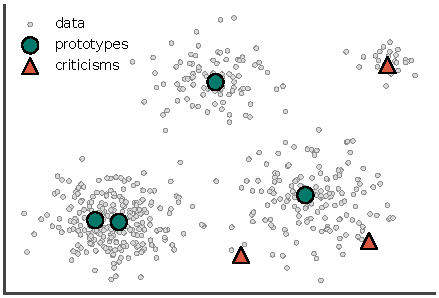
\includegraphics[width=0.58\textwidth]{ch03/mmd_critic}
\caption{Prototypes and criticisms selected by MMD-critic on a two-dimensional data set.}
\label{fig:mmd}
\end{figure}

\subsection{Influential instances}

A training instance is \emph{influential\index{influential instance|textbf}} if deleting it considerably changes the parameters or the
predictions of the model. With influential instances we do not treat the model as fixed but as a
function of the training data, which helps to debug it: we learn for which instances the model could
have problems, which training instances should be checked for errors, and how robust the model is. We
might not trust a model whose parameters depend strongly on a single instance.

An influential instance is not the same as an \emph{outlier}, an instance far from the others: an
outlier is influential only if it changes the model, which also depends on its target value.
\emph{Deletion diagnostics\index{deletion diagnostics|textbf}} retrain the model without each instance $i$ and measure the change:
\begin{equation}
  \mathrm{DFBETA}_i=\beta-\beta^{(-i)},\qquad
  D_i=\frac{\sum_{j=1}^{n}\bigl(\hat y_j-\hat y_j^{(-i)}\bigr)^2}{p\cdot\mathrm{MSE}},
\end{equation}
where $\beta^{(-i)}$ and $\hat y_j^{(-i)}$ are the parameters and predictions of the model trained without
instance $i$, and $D_i$ is \emph{Cook's distance\index{Cook's distance|textbf}} \citep{cook1977detection}, with $p$ parameters. DFBETA
needs a model with parameters; Cook's distance does not, but the MSE\index{mean squared error (MSE)} is not meaningful for every model,
and the simplest model-agnostic measure is the mean absolute change of the predictions. We can also
measure the influence of each training instance on the prediction for a particular instance, and model
the influence as a function of the features (for instance, with a short tree) to find out what kind of
training instances are most influential.

\begin{pylisting}[label={lst:influence}]{Deletion diagnostics: DFBETA and Cook's distance}
import numpy as np
from sklearn.linear_model import LinearRegression

rng = np.random.default_rng(7)
x = np.r_[rng.uniform(0, 5, 30), 12.0]                  # last point: high leverage...
y = np.r_[2 * x[:30] + 1 + rng.normal(0, 1.2, 30), 6.0] # ...and off the trend
X = x[:, None]
full = LinearRegression().fit(X, y)
yhat = full.predict(X)
s2 = np.sum((y - yhat) ** 2) / (len(y) - 2)              # residual variance (2 parameters)
dfbeta, cook = [], []
for i in range(len(y)):                       # deletion diagnostics: refit without i
    m = LinearRegression().fit(np.delete(X, i, 0), np.delete(y, i))
    dfbeta.append(full.coef_[0] - m.coef_[0])
    cook.append(np.sum((yhat - m.predict(X)) ** 2) / (2 * s2))
for i in np.argsort(cook)[::-1][:3]:
    print(f"instance {i:2d}: x={x[i]:5.2f}  DFBETA={dfbeta[i]:+.3f}  "
          f"Cook's D={cook[i]:.3f}")
\end{pylisting}
\begin{pyoutput}
instance 30: x=12.00  DFBETA=-1.237  Cook's D=17.473
instance 19: x= 4.94  DFBETA=+0.078  Cook's D=0.140
instance 16: x= 4.98  DFBETA=+0.059  Cook's D=0.080
\end{pyoutput}

In \cref{lst:influence} and \cref{fig:influence}, a single instance with an extreme value of $x$ that
does not follow the trend changes the slope of a regression from 2.12 to 0.88; its Cook's distance is
17.5, while the next largest is 0.14.

\begin{figure}[htbp]
\centering
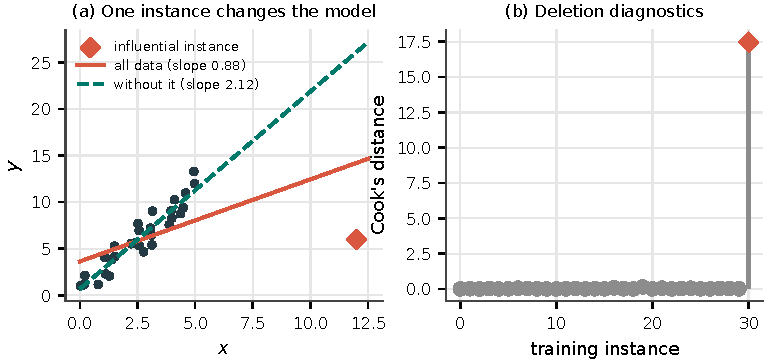
\includegraphics[width=\textwidth]{ch03/influence}
\caption{(a) A linear regression with and without one influential instance. (b) Cook's distance of each
training instance.}
\label{fig:influence}
\end{figure}

Deletion diagnostics are expensive, because the model must be retrained once per instance.
\emph{Influence functions\index{influence function|textbf}} \citep{koh2017understanding} approximate them for models with differentiable
losses: upweighting an instance $z$ by an infinitesimal $\epsilon$ changes the parameters by
approximately
\begin{equation}
  \hat\theta_{\epsilon,z}-\hat\theta\approx-\epsilon\,H_{\hat\theta}^{-1}\nabla_\theta L(z,\hat\theta),
\end{equation}
the gradient of the loss of $z$ scaled by the inverse Hessian $H_{\hat\theta}$ of the training loss (the
curvature). Here the training loss is the average $\frac1n\sum_iL(z_i,\theta)$ and $z$ receives the extra
weight $\epsilon$; removing $z$ corresponds to $\epsilon=-1/n$, which reverses the sign:
$\hat\theta_{-z}-\hat\theta\approx\frac1n H_{\hat\theta}^{-1}\nabla_\theta L(z,\hat\theta)$. The approximation
requires a regular optimum with an invertible Hessian. Influential instances are among the best debugging tools: they reveal the weaknesses of a
model, help to handle domain mismatch between training and test data (which training instances caused an
error?), tell us which training labels to check first when we cannot check them all, and can be compared
across models. Influence functions can even be used to create adversarial training\index{adversarial training} data. Their limits:
they only consider single instances, there is no clear cut-off for calling an instance influential, and
influence functions are an approximation, validated mostly empirically.

\subsection{The future of interpretability}

Interpretability tools catalyse the adoption of machine learning: since the goal of a model can never be
specified perfectly, interpretability is needed to close the gap between the specified and the actual
goal, and many organisations and industries demand transparency for legal reasons, for risk aversion or
to gain insight. The focus is moving towards model-agnostic tools, interpretability is being automated
along with model building (Unit~4), and systems are increasingly expected to explain themselves.
Regulation pushes in the same direction: the debate on whether the European data protection regulation
grants a ``right to explanation\index{right to explanation}'' of automated decisions \citep{goodman2017european,wachter2018counterfactual}
was followed by the European Artificial Intelligence Act \citep{eu2024aiact}, which imposes transparency,
documentation and human oversight requirements on high-risk\index{AI Act!high-risk systems} systems.

% =====================================================================
\section{Machine learning and security}\label{sec:security}

As soon as enough computers were connected, some people realised that the network was a perfect
medium to make money, often illegitimately. Spam is the classic example, and it shows both the
promise and the difficulty of using machine learning in security \citep{chio2018machine}. Machine
learning was not invented by spam fighters, but it was quickly adopted by those who saw its potential
against a constantly evolving source of abuse. Content-based\index{content-based filtering} models learned from e-mail data recognise
spam in a generalisable way; metadata and the reputation of senders add evidence; and a feedback loop
with users, who mark messages as spam, builds a collective intelligence that improves over time. Spam
filters have evolved to deal with an ever-growing diversity\index{diversity} of circumvention methods, and today the vast
majority of spam never reaches the inbox, although most e-mail traffic is spam. But the story also
shows the essential feature of security: a \emph{motivated adversary} constantly tries to misuse the
system, and each side races to exploit or fix the flaws before the other finds them.

The motivation of attackers today is largely monetary. Underground marketplaces sell vulnerabilities,
stolen accounts and easy-to-use attack tools, so that attacks no longer require great technical skill;
the trade in previously unknown (``zero-day'') vulnerabilities exists both legally and illegally. As long
as attacks generate profit, there will be people willing to launch them.

\subsection{Uses and limitations of machine learning in security}

The uses of machine learning in security fall into two broad categories:
\begin{itemize}
  \item \emph{pattern recognition}: discover the explicit or latent characteristics of known kinds of
        malicious data, distil\index{model distillation} them into features, and recognise other data that share them (malware,
        bots, spam, phishing);
  \item \emph{anomaly detection}: establish a notion of normality that describes most of the data (say,
        more than 95\%), and flag any deviation (network intrusion detection, access control, user
        authentication); see \cref{sec:unsupervised}.
\end{itemize}
The limitations are equally important: the results often need to be explained to analysts; much of the
context of an attack comes from cultural and experiential knowledge that is not in the data; models
overfit to past attacks; and, above all, the data are generated by adversaries who adapt to the model.
Machine learning should be approached with equal parts of enthusiasm and caution.

% ---------------------------------------------------------------------
\section{Adversarial machine learning}\label{sec:adversarial}

As machine learning is deployed in critical systems, its reliability comes under scrutiny, and the
system itself can be targeted to serve the goals of an attacker. \emph{Adversarial machine learning\index{adversarial machine learning|textbf}}
studies the vulnerabilities of machine learning in adversarial environments
\citep{huang2011adversarial,biggio2018wild}. Vulnerabilities can arise from flawed system design, from
fundamental limitations of the algorithms, or from a combination of both, and designers of systems on
which security, sovereignty or lives depend have a responsibility to anticipate attacks.

\subsection{A taxonomy of attacks}

Attacks are classified along three axes \citep{barreno2006can,huang2011adversarial}
(\cref{tab:attacks}).

\begin{table}[htbp]
\centering\small
\caption{A taxonomy of attacks on machine learning systems.}\label{tab:attacks}
\begin{tabularx}{\textwidth}{@{}>{\raggedright\arraybackslash}p{2.6cm}>{\raggedright\arraybackslash}X>{\raggedright\arraybackslash}X@{}}
\toprule
Axis & & \\
\midrule
Influence & \emph{causative}: tamper with the training data or process; relevant above all for
\emph{online} learners, which are retrained continuously with fresh data & \emph{exploratory}: interact
with the trained model to find inputs that it misclassifies (for instance, by brute-force fuzzing of its
input space)\\
Specificity & \emph{targeted}: shift predictions towards a specific outcome (malware of family A
classified as family B) & \emph{indiscriminate}: make the model wrong, whatever the outcome (family A
classified as any other)\\
Security violation & \emph{integrity}: reduce the ability of the detector to find attacks (lower true
positive rate), so that the attack gets through & \emph{availability}: make the system unusable by
degrading it so much (false alarms, missed detections) that its results cannot be acted upon\\
\bottomrule
\end{tabularx}
\end{table}

The power of an attacker also depends on its \emph{knowledge}: a white-box attacker knows everything about
the model (type, parameters, training data); a grey-box attacker knows part of it (for instance, the
features); and a black-box attacker can only query the model. Even a black-box attacker who sees only the
predicted labels can infer the decision boundary by querying points around it; one who also sees the
predicted probabilities is in a much stronger position.

\paragraph{Why are machine learning systems vulnerable?} Machine learning techniques are usually
developed assuming that the training and deployment\index{deployment} data come from the same distribution, an
assumption that an adversary will try to break whenever that is the path of least resistance. Learning is also
\emph{imperfect}: the training data are drawn from an incomplete part of the space of possible inputs,
the model makes simplifying assumptions, and even the best classifier has an irreducible (Bayes) error.
The regions of the input space that the training data do not cover, between the data the model has
fitted and everything that could be presented to it, form an \emph{adversarial space} that attackers can
exploit.

\paragraph{Transferability} Adversarial examples\index{adversarial example} crafted for one model are often also misclassified by
other, independently trained models, even with different algorithms and training sets
\citep{szegedy2014intriguing,papernot2016transferability}: the adversarial spaces of different models
overlap. This makes practical black-box attacks possible, because the attacker can build a surrogate\index{global surrogate}
model with queries (\cref{sec:drawbacks}), study it offline, and attack the real system with the
adversarial examples it finds \citep{papernot2017practical}. Model parameters are rarely exposed, but
that is not enough protection.

\subsection{Poisoning attacks}

\emph{Poisoning\index{poisoning attack|textbf}} is a causative attack, relevant to systems that keep learning after deployment. Anomaly
detectors, for instance, are retrained automatically to follow the changes in the data distribution
without human intervention\index{intervention}; online systems sacrifice stationarity for adaptability. An attacker who
controls part of the training data can then inject carefully placed synthetic examples, called
\emph{chaff}, to move the decision boundary (a \emph{red herring}), either in a targeted way (so that one
kind of attack is accepted) or indiscriminately \citep{biggio2012poisoning}. The more data the
attacker controls, the more successful the attack, so popular services, which see a large volume of
legitimate traffic, are harder to poison. A sudden flood of strange training data is easy to notice, but
a \emph{boiling frog} attack, executed gradually over a long period, can look like organic drift.

\begin{pylisting}[label={lst:poisoning}]{A red-herring poisoning attack on a spam detector}
import numpy as np
from sklearn.linear_model import LogisticRegression

def emails2d(n, seed):                        # two features that summarise each e-mail
    rng = np.random.default_rng(seed)
    X = np.r_[rng.normal([-1.2, -1.2], 1.0, (n, 2)), rng.normal([1.2, 1.2], 1.0, (n, 2))]
    return X, np.r_[np.zeros(n, int), np.ones(n, int)]                # 1 = spam

X, y = emails2d(1000, 0)
X_test, y_test = emails2d(5000, 1)
print("chaff   spam caught   ham flagged   uncertain (0.4 < p < 0.6)")
for frac in (0.0, 0.05, 0.1, 0.2):
    k = int(frac * len(y))
    # chaff: spam-like points labelled as ham (a larger attack adds to a smaller one)
    chaff = np.random.default_rng(2).normal([1.0, 1.0], 0.35, (k, 2))
    model = LogisticRegression().fit(np.r_[X, chaff], np.r_[y, np.zeros(k, int)])
    p = model.predict_proba(X_test)[:, 1]
    caught, flagged = np.mean(p[y_test == 1] >= 0.5), np.mean(p[y_test == 0] >= 0.5)
    band = np.mean((p > 0.4) & (p < 0.6))
    print(f"{frac:4.0%}      {caught:.3f}         {flagged:.3f}         {band:.3f}")
\end{pylisting}
\begin{pyoutput}
chaff   spam caught   ham flagged   uncertain (0.4 < p < 0.6)
  0%      0.958         0.040         0.019
  5%      0.916         0.018         0.046
 10%      0.869         0.011         0.063
 20%      0.777         0.005         0.095
\end{pyoutput}

\Cref{lst:poisoning} and \cref{fig:poisoning} simulate an attack on a detector retrained with fresh
data. The attacker injects spam-like messages labelled as legitimate close to the spam side of the
boundary. With chaff amounting to 10\% of the training data the detector catches 86.9\% of the spam
instead of 95.8\%, and with 20\% only 77.7\%; at the same time it flags fewer legitimate messages, so an
operator who looks only at complaints about false alarms would see an \emph{improvement}. The fraction of
predictions in the uncertain band $0.4<p<0.6$, however, grows from 1.9\% to 9.5\%, because the attacker
works close to the boundary.

\begin{figure}[htbp]
\centering
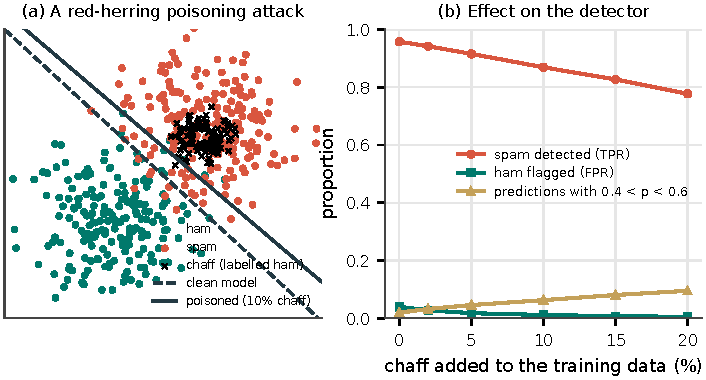
\includegraphics[width=\textwidth]{ch03/poisoning}
\caption{(a) Poisoning moves the decision boundary of a spam detector towards the spam. (b) Detection
rate, false alarm rate and fraction of uncertain predictions as the amount of chaff grows.}
\label{fig:poisoning}
\end{figure}

\paragraph{Attacker knowledge} Knowing the decision function is an important factor: where to place the
chaff, and how much is needed to move the boundary meaningfully, can be hard to determine when the input
is transformed before reaching the classifier (for instance, by a dimensionality reduction). With enough
access, these difficulties can mostly be overcome; the defender's goal is to make such inference
difficult without sacrificing the efficacy of the system.

\paragraph{Defences} There are significant benefits in designing online learning systems that behave
like periodic batch systems: longer periods between retraining give time to inspect the data, a longer
history makes boiling-frog attacks easier to detect, and attackers thrive on short feedback loops.
Poisoning attempts can also be detected by looking for abnormal pockets of traffic (coming from the same
addresses or networks, or sharing unusual characteristics); by keeping a \emph{calibration\index{calibration|textbf} set} of
handcrafted normal and malicious data on which every retrained model is tested; and by monitoring\index{monitoring} the
fraction of predictions that fall near the decision boundary, as in \cref{fig:poisoning}b: a sudden rise
(say, from 30\% to 80\% of the points in the band) suggests that someone is pushing the boundary. There is
no definitive recipe; this is an active area of research, and monitoring is the subject of Unit~6.

\subsection{Evasion attacks}

\emph{Evasion\index{evasion attack|textbf}} is an exploratory attack: the attacker finds adversarial examples\index{adversarial example} that the deployed model
misclassifies, without any influence on its training. Evasion affects every kind of classifier,
traditional and deep, and can have real-world consequences, from road signs to malware detection
\citep{biggio2013evasion}. Perturbations are easy to apply to images, where changing a few pixel
intensities is invisible; applying them to executables is harder, because the modified binary must remain
valid and keep its malicious behaviour, but it has been done.

\begin{pylisting}[label={lst:fgsm}]{FGSM on handwritten digits: white box, transfer and adversarial training}
import numpy as np
from sklearn.datasets import load_digits
from sklearn.ensemble import RandomForestClassifier
from sklearn.linear_model import LogisticRegression
from sklearn.model_selection import train_test_split
from sklearn.neural_network import MLPClassifier

X, y = load_digits(return_X_y=True)
X = X / 16.0                                                    # pixels in [0, 1]
X_tr, X_te, y_tr, y_te = train_test_split(X, y, test_size=0.4, random_state=0, stratify=y)

def fgsm(model, X, y, eps):
    """Fast gradient sign method for a softmax (multinomial logistic) model."""
    P = model.predict_proba(X)
    P[np.arange(len(y)), y] -= 1.0                              # d loss / d logits
    grad = P @ model.coef_                                       # d loss / d input
    return np.clip(X + eps * np.sign(grad), 0, 1)

lr = LogisticRegression(max_iter=3000).fit(X_tr, y_tr)
mlp = MLPClassifier((100,), max_iter=1000, random_state=0).fit(X_tr, y_tr)
rf = RandomForestClassifier(300, random_state=0).fit(X_tr, y_tr)
robust = LogisticRegression(max_iter=3000).fit(np.r_[X_tr, fgsm(lr, X_tr, y_tr, 0.15)],
                                               np.r_[y_tr, y_tr])    # adversarial training
print("eps   LR (white  MLP (trans-  RF (trans-  robust LR:   robust LR:")
print("      box)       ferred)      ferred)     old attack   adaptive")
for eps in (0.0, 0.05, 0.1, 0.2):
    Xa = fgsm(lr, X_te, y_te, eps)                   # crafted on the original LR
    Xr = fgsm(robust, X_te, y_te, eps)               # crafted on the robust LR itself
    print(f"{eps:.2f}  {lr.score(Xa, y_te):.3f}      {mlp.score(Xa, y_te):.3f}        "
          f"{rf.score(Xa, y_te):.3f}       {robust.score(Xa, y_te):.3f}        "
          f"{robust.score(Xr, y_te):.3f}")
\end{pylisting}
\begin{pyoutput}
eps   LR (white  MLP (trans-  RF (trans-  robust LR:   robust LR:
      box)       ferred)      ferred)     old attack   adaptive
0.00  0.972      0.979        0.971       0.940        0.940
0.05  0.873      0.851        0.892       0.940        0.720
0.10  0.641      0.534        0.627       0.926        0.325
0.20  0.090      0.032        0.241       0.871        0.006
\end{pyoutput}

\Cref{lst:fgsm} and \cref{fig:adversarial} attack a logistic regression trained on images of handwritten
digits with the fast gradient sign\index{fast gradient sign method (FGSM)} method of \cref{eq:fgsm}. Changing every pixel by 0.1 (on a 0--1
scale) reduces its accuracy from 0.972 to 0.641, and by 0.2 to 0.090. The same adversarial images,
crafted only with the logistic regression, also fool a neural network (0.534 at $\epsilon=0.1$) and a
random forest (0.627), neither of which the attacker has seen: this is transferability.

\begin{figure}[htbp]
\centering
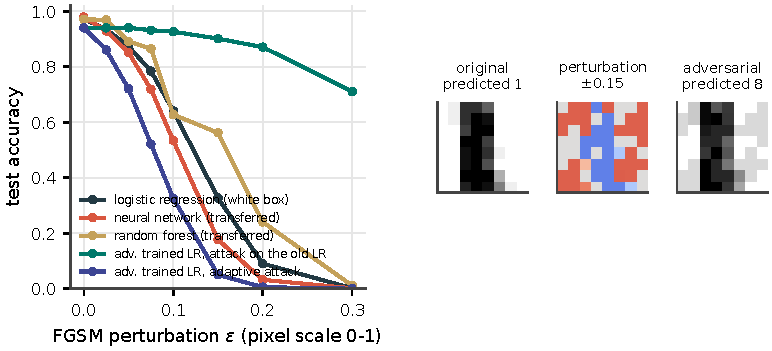
\includegraphics[width=\textwidth]{ch03/adversarial_digits}
\caption{Evasion with the fast gradient sign method on handwritten digits. Left: accuracy as a function
of the size of the perturbation, for the attacked model, two models that receive the transferred
examples, and an adversarially trained model. Right: an image, the perturbation and the adversarial image.}
\label{fig:adversarial}
\end{figure}

\paragraph{Defences} There are no robust general defences against evasion. The general idea is to make it
harder for the attacker to obtain information about the gradients of the decision surface:
\begin{itemize}
  \item \emph{adversarial training\index{adversarial training|textbf}} adds adversarial examples with their correct labels to the training
        data \citep{goodfellow2015explaining}, ideally generating them against the current model at every
        step of training \citep{madry2018towards}. It tries to cover the parts of the input space that the
        training data do not reach, which can never be done exhaustively. In \cref{lst:fgsm}, a model
        trained once with adversarial images is robust to the attack it was trained on (0.871 at
        $\epsilon=0.2$), but an attacker who crafts new examples against \emph{it} breaks it completely
        (0.006): the defence only raised the bar for an attacker who does not adapt;
  \item \emph{defensive distillation\index{model distillation|textbf}} \citep{papernot2016distillation} trains a second model on the
        probability outputs of the first (the distillation of \cref{sec:drawbacks}), which smooths the
        decision surface and hides useful gradients; stronger attacks were soon shown to defeat it
        \citep{carlini2017towards}. More generally, defences that merely mask the gradients give a false
        sense of security \citep{athalye2018obfuscated}.
\end{itemize}
Many practical defences fail against adaptive attacks, so robustness must be evaluated under an explicit threat
model\index{threat model} and attack budget. A defence may raise the cost of attacks or provide guarantees within stated constraints;
neither establishes security against every possible adversary.

\begin{example}{A good-word attack on a spam filter}{goodword}
A spammer cannot see the filter but can test messages against it. \citet{lowd2005good} showed that adding
a few ``good'' words, typical of legitimate e-mail, is enough to get much spam through statistical filters.
\Cref{lst:goodword} simulates the attack on a logistic regression filter over a vocabulary of 60 words:
the attacker greedily adds the word that most lowers the spam probability, one query per candidate word.
Three added words let 36\% of the detected spam through, five words 67\%, and ten words 98\%. Retraining the
filter with attacked spam labelled as spam makes the attack harder (23\%, 55\% and 95\%) without stopping
it (\cref{fig:evasion}).
\end{example}

\begin{pylisting}[label={lst:goodword}]{A black-box good-word attack and adversarial training}
import numpy as np
from sklearn.linear_model import LogisticRegression

def emails(n, seed):
    """Bag of words: words 0-14 are 'spammy', 15-29 'hammy' and 30-59 neutral."""
    rng = np.random.default_rng(seed)
    spam = np.r_[np.ones(n // 2, int), np.zeros(n - n // 2, int)]
    p = np.where(spam[:, None] == 1, [0.30] * 15 + [0.05] * 15 + [0.1] * 30,
                 [0.03] * 15 + [0.25] * 15 + [0.1] * 30)
    return (rng.random((n, 60)) < p).astype(float), spam

def good_word_attack(model, x, budget=10):
    """Add, one at a time, the word that most lowers P(spam) (one query per candidate)."""
    x = x.copy()
    for k in range(budget + 1):
        if model.predict_proba(x[None])[0, 1] < 0.5:
            return k, x
        if k == budget:
            return None, x
        cand = np.flatnonzero(x == 0)
        Z = np.repeat(x[None], len(cand), axis=0)
        Z[np.arange(len(cand)), cand] = 1
        x[cand[np.argmin(model.predict_proba(Z)[:, 1])]] = 1

X, y = emails(4000, 0)
X_test, y_test = emails(2000, 1)
clf = LogisticRegression(max_iter=2000).fit(X, y)
adv = np.array([good_word_attack(clf, x)[1] for x in X[y == 1][:600]])
X_aug, y_aug = np.r_[X, adv], np.r_[y, np.ones(len(adv), int)]     # attacked spam is spam
robust = LogisticRegression(max_iter=2000).fit(X_aug, y_aug)
for name, m in [("standard filter", clf), ("adversarially trained", robust)]:
    caught = X_test[(y_test == 1) & (m.predict(X_test) == 1)][:300]
    need = [good_word_attack(m, x)[0] for x in caught]
    rates = [np.mean([k is not None and k <= b for k in need]) for b in (1, 3, 5, 10)]
    det = m.predict(X_test)[y_test == 1].mean()
    print(f"{name:22s} detection={det:.3f}  evasion with 1/3/5/10 words: "
          + " ".join(f"{r:.2f}" for r in rates))
\end{pylisting}
\begin{pyoutput}
standard filter        detection=0.974  evasion with 1/3/5/10 words: 0.06 0.36 0.67 0.98
adversarially trained  detection=0.974  evasion with 1/3/5/10 words: 0.04 0.23 0.55 0.95
\end{pyoutput}

\begin{figure}[htbp]
\centering
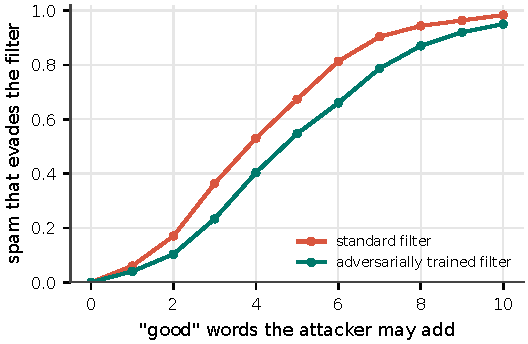
\includegraphics[width=0.66\textwidth]{ch03/evasion}
\caption{Fraction of detected spam that evades the filter as a function of the number of good words the
attacker may add, for a standard and an adversarially trained filter.}
\label{fig:evasion}
\end{figure}

\subsection{Other threats}

Poisoning\index{poisoning attack} and evasion\index{evasion attack} are not the only threats. A model offered through an API\index{API} can be \emph{stolen} by
querying it and training a copy \citep{tramer2016stealing}; \emph{membership inference} attacks find out
whether a given record was part of the training data, a privacy breach for medical or financial data
\citep{shokri2017membership}; \emph{backdoors\index{backdoor criterion|textbf}} hidden in training data or in pre-trained models make a
model misbehave only when a secret trigger is present \citep{gu2017badnets}; and applications built on
large language models\index{large language model (LLM)}\index{language model} can be hijacked by instructions hidden in the content they process, a \emph{prompt\index{prompt|textbf}
injection\index{prompt injection|textbf}} \citep{greshake2023not}.

\begin{keyidea}
Being secure and robust is a prerequisite for deploying machine learning, but the difficulty of avoiding
attacks is not a reason to shy away from it. Machine learning can behave in unexpected ways in adversarial
environments; this is not a ``failure'' of machine learning but a sign of improperly calibrated
expectations. Knowing the types of vulnerability helps to make fewer false assumptions about what a model
can do.
\end{keyidea}

% ---------------------------------------------------------------------

% =====================================================================
\section{Regulation: the European AI Act}\label{sec:aiact}

Much of what this unit has presented as good practice is now law in the European Union. Regulation (EU)
2024/1689, the \emph{AI Act\index{AI Act|textbf}}, entered into force on 1 August 2024 as the first comprehensive law on artificial
intelligence \citep{eu2024aiact}. It does not regulate techniques but \emph{uses}: the same classifier may be
unregulated when it filters spam and heavily regulated when it decides who gets a loan. It complements earlier
rules, such as the General Data Protection Regulation\index{GDPR}, which already gives people the right not to be subject
to decisions based solely on automated processing that significantly affect them, with safeguards such as
human intervention\index{intervention} \citep{gdpr2016,wachter2017right}. For decisions based on the output of the high-risk\index{AI Act!high-risk systems} systems of Annex~III\index{AI Act!Annex III}
(except those of its point~2, critical infrastructure) that produce legal effects, or similarly significantly affect a
person in a way that they consider adverse to their health, safety or fundamental rights, the AI Act adds a right to
obtain clear and meaningful explanations of the role of the system in the decision procedure and of the main elements
of the decision (Article~86\index{AI Act!Article 86}), subject to the exceptions and restrictions of other laws. It is not a general obligation
to produce actionable or counterfactual explanations\index{counterfactual explanation} for every decision.

\subsection{A risk-based approach}

The AI Act\index{AI Act} sorts AI systems into four levels of risk:
\begin{itemize}
  \item \emph{unacceptable risk}: practices that are prohibited, such as manipulating people by exploiting
        their vulnerabilities, social scoring, predicting that a person will commit a crime solely from their
        profile, building facial recognition databases by untargeted scraping of images, recognising emotions in
        workplaces and schools, inferring sensitive attributes\index{protected attribute} such as religion or sexual orientation from
        biometric data, and, with narrow exceptions, real-time remote biometric identification in public spaces
        for law enforcement;
  \item \emph{high risk\index{AI Act!high-risk systems|textbf}}: systems that are safety components of products already regulated in the EU (medical
        devices, machinery, toys) and systems used in the areas listed in Annex~III\index{AI Act!Annex III} of the Act: biometrics,
        critical infrastructure, education (admission, assessment), employment (recruitment, promotion,
        monitoring of workers), access to essential services (eligibility for public benefits, the
        creditworthiness and credit scoring of people, risk assessment and pricing in life and health insurance,
        triage of emergency calls), law enforcement, migration and border control, and the administration of
        justice and democratic processes;
  \item \emph{limited risk}: systems subject to transparency obligations: people must be told when they are
        interacting with a chatbot, and content generated or manipulated by AI, such as deepfakes, must be
        labelled as such;
  \item \emph{minimal risk}: everything else, such as spam filters or film recommenders\index{recommender system}, with no specific
        obligations beyond the duty to take measures that support the \emph{AI literacy\index{AI literacy|textbf}} of the staff who use
        AI (as amended in 2026, Article~4 does not require guaranteeing a specific individual level).
\end{itemize}
\emph{General-purpose AI models}, such as large language models\index{large language model (LLM)}, have their own obligations: technical documentation,
information for the providers that build systems on them, a policy to respect copyright and a summary of the
content used for training; the most capable ones, presumed to pose systemic risks, must also be evaluated, including
adversarial testing, have their serious incidents reported, and be adequately protected.

\subsection{Obligations for high-risk systems}

The \emph{providers} of high-risk\index{AI Act!high-risk systems} systems, those who develop them or place them on the market, must meet a set of
requirements before and after the system is deployed. Read with the eyes of a data scientist, they are a summary of this
book (\cref{tab:aiact}). The \emph{deployers}, the organisations that use the systems, must use them according to their
instructions, assign human oversight to competent people, make sure that the input data are relevant, monitor their
operation and keep their logs; public bodies, and those that use AI for credit scoring or to price life and health
insurance, must also assess the impact of the system on fundamental rights before using it.

\begin{table}[htbp]
\centering\small
\caption{Requirements of the AI Act for high-risk systems, and where this book deals with them.}\label{tab:aiact}
\begin{tabularx}{\textwidth}{@{}>{\raggedright\arraybackslash}p{3.0cm}>{\raggedright\arraybackslash}X>{\raggedright\arraybackslash}p{3.1cm}@{}}
\toprule
Requirement & What it asks for & In this book\\
\midrule
Risk management (Art.~9) & identify, estimate and mitigate the risks of the system throughout its life cycle & Units
\ref{ch:evaluation}, \ref{ch:reliable} and \ref{ch:monitoring}\\
Data governance (Art.~10) & relevant and representative training, validation and test data, examined for possible
biases & \cref{sec:protocols,sec:fairness,sec:shift}\\
Documentation and logs (Arts.~11--12) & technical documentation of the system, and automatic recording of its operation
& model cards \citep{mitchell2019model}; \cref{sec:infrastructure}\\
Transparency (Art.~13) & instructions that let deployers understand the system and use its outputs appropriately &
\cref{sec:interpretability}\\
Human oversight (Art.~14) & people able to understand, monitor, override and stop the system, aware of the tendency to
over-rely on it & \cref{sec:cautious}; \cref{sec:interpretability}\\
Accuracy, robustness, cybersecurity (Art.~15) & declared levels of accuracy, resilience to errors and to attacks such as
poisoning and adversarial examples & \cref{ch:evaluation}; \cref{sec:adversarial}\\
Quality management and conformity (Arts.~17, 43) & documented processes, and an assessment of conformity before the system
is placed on the market & \cref{sec:infrastructure}\\
Post-market monitoring (Arts.~72--73) & collect and analyse data on the performance of the system in use, and report
serious incidents & \cref{ch:monitoring}\\
\bottomrule
\end{tabularx}
\end{table}

\subsection{Timeline and enforcement}

The obligations apply in stages. The prohibitions and the duty to support AI literacy\index{AI literacy} apply since 2 February 2025, and the
obligations for general-purpose models since 2 August 2025. The obligations for high-risk\index{AI Act!high-risk systems} systems were due to apply from
August 2026, but an amendment adopted in 2026, the \emph{Digital Omnibus\index{Digital Omnibus on AI|textbf} on AI} (Regulation (EU) 2026/1744, in force since 27 July 2026),
postponed them to fixed dates: those for the systems of Annex~III\index{AI Act!Annex III}, such as credit scoring, apply from 2 December 2027, and those for systems
embedded in regulated products from 2 August 2028 \citep{eu2026omnibus}. The amendment also widened the possibility of
processing personal data when strictly necessary to detect and correct biases, which matters because, as we saw in
\cref{sec:fairness}, measuring discrimination usually requires the very attributes that one would like to leave out. Fines
reach 35 million euros or 7\% of a company's worldwide annual turnover for prohibited practices, and 15 million euros or 3\% for
other infringements. Each member state designates authorities to supervise the market; Spain created the first national
agency, the Spanish Agency for the Supervision of Artificial Intelligence (AESIA), while the European Commission's AI Office
supervises general-purpose models. This section describes the AI Act\index{AI Act} as amended in 2026, as checked on 12 October 2026;
its obligations and dates must be rechecked for each edition.

\subsection{A credit-scoring model under the AI Act}

Consider the credit model of \cref{sec:fairness} in a European bank. It is a high-risk\index{AI Act!high-risk systems} system, so before using it the bank, as
its provider, must document its data and their representativeness, its performance overall and for the relevant groups of
applicants (\cref{lst:credit}), its known limitations and the conditions under which it should not be used. Its decisions must be
logged, and a person must be able to review and override them: the cautious classifiers\index{cautious classifier} of \cref{sec:cautious}, which
delegate\index{delegation} uncertain cases to an analyst, are a natural design. Rejected applicants may have the right to a clear and meaningful
explanation of the role of the system in the decision (Article~86\index{AI Act!Article 86}); offering an explanation they can act on, such as the
counterfactual explanations\index{counterfactual explanation} of \cref{sec:examplebased} (``with a debt ratio below 35\%, the loan would have been approved''),
is a design choice that goes beyond that right. Once in use, the model must be monitored for drift and for changes in its performance across groups, and serious
incidents must be reported (\cref{ch:monitoring}). None of these obligations requires a new technique; all of them require using the
techniques of this book systematically, and documenting that they were used. The techniques help to meet the
obligations, but they do not replace conformity assessment, legal documentation and the procedures the law requires.

\begin{keyidea}
The AI Act\index{AI Act} regulates what a system is used for, not how it is built. For high-risk uses it turns evaluation, data governance,
documentation, human oversight, robustness and monitoring from good practice into legal obligations.
\end{keyidea}

% =====================================================================
\section{Summary}\label{sec:summary3}

\begin{itemize}
  \item Unfairness can enter a machine learning system at every stage: measurement, learning, action and
        feedback. Removing the sensitive attribute\index{protected attribute} does not remove it.
  \item The main group fairness\index{fairness} criteria (independence, separation\index{fairness!separation} and sufficiency\index{fairness!sufficiency}) are conditional
        independences that are generally incompatible; choosing one is choosing whose errors matter. They
        are diagnostics, not certificates, and they cannot distinguish mechanisms with the same
        observational distribution.
  \item Causal models distinguish observing from intervening. Confounders\index{confounder} must be adjusted for, mediators\index{mediator}
        and colliders\index{collider} must not; counterfactuals answer questions about alternatives to what happened. Both
        are needed to reason about discrimination.
  \item Interpretability is needed because objectives are never completely specified. Interpretable models
        (linear, logistic, trees, rules) can be read directly, with care about their assumptions.
  \item Model-agnostic methods (PDP, ICE\index{individual conditional expectation}, interaction strength, permutation importance\index{feature importance!permutation}, surrogates\index{global surrogate}, LIME\index{LIME} and
        Shapley\index{Shapley values} values) explain any model, but each answers a different question and has limitations that
        must be known.
  \item Example-based explanations (counterfactuals, prototypes\index{prototypes and criticisms} and criticisms, influential instances\index{influential instance})
        explain with instances; adversarial examples\index{adversarial example} are counterfactuals designed to deceive.
  \item Machine learning systems can be attacked during training (poisoning\index{poisoning attack}) and deployment (evasion\index{evasion attack});
        adversarial examples transfer between models, and defences raise the cost of attacks without
        eliminating them.
  \item The European AI Act\index{AI Act} regulates uses by their risk: it prohibits some practices and, for high-risk\index{AI Act!high-risk systems} systems such as
        credit scoring, requires risk management, data governance, documentation, logging, transparency, human oversight,
        accuracy, robustness and monitoring after deployment.
\end{itemize}

\section*{Bibliographic notes}
\phantomsection\addcontentsline{toc}{section}{Bibliographic notes}

The fairness\index{fairness} and causality\index{causality} sections follow the approach of \citet{barocas2023fairness}, whose book is the
best introduction to the field; \citet{mehrabi2021survey} survey the sources of bias and the mitigation
techniques. \citet{pearl2018book} is an accessible introduction to causal reasoning, and
\citet{pearl2009causality}, \citet{peters2017elements} and \citet{hernan2020causal} are more technical
references. The interpretability sections follow \citet{molnar2022interpretable}, which describes many more
methods; \citet{miller2019explanation} reviews what the social sciences say about explanations and
\citet{doshivelez2017towards} discuss how to evaluate interpretability. \citet{chio2018machine} cover machine
learning for security, and \citet{biggio2018wild} review ten years of adversarial machine learning\index{adversarial machine learning}.

\section*{Exercises}
\phantomsection\addcontentsline{toc}{section}{Exercises}

\begin{enumerate}[label=\textbf{3.\arabic*},ref=3.\arabic*,leftmargin=*,itemsep=6pt]
  \item\label{exr3:groups} A hiring model is applied to 600 candidates of group $a$ (400 qualified) and 400
        of group $b$ (160 qualified). It selects 300 qualified and 40 unqualified candidates of group $a$,
        and 96 qualified and 24 unqualified of group $b$. Compute, for each group, the selection rate, the
        true and false positive rates\index{false positive rate} and the positive predictive value\index{predictive value!positive}. Does the model pass the
        four-fifths rule? Which criteria hold?
  \item\label{exr3:chouldechova} Two groups have prevalences\index{prevalence} 0.6 and 0.3. A classifier has $\PPV=0.8$ and
        $\TPR=0.7$ in both groups. Use \cref{eq:chouldechova} to compute the false positive rate of each
        group.
  \item\label{exr3:simpson} Department X admits 80 of 100 men and 18 of 20 women; department Y admits 4 of
        20 men and 30 of 100 women. Compute the aggregate admission rates and the rates adjusted with the
        overall distribution of applicants across departments.
  \item\label{exr3:heart} In the heart disease model of \cref{ex:heart}, change the probabilities to
        $P(U_1=1)=0.4$, $P(U_2=1)=0.5$ and $P(U_3=1)=0.25$. Compute $P(H=1)$, $P(H=1\mid W=1)$ and
        $P(H=1\mid\mathrm{do}(W:=1))$.
  \item\label{exr3:adjust} In a causal graph\index{causal graph}, age $Z$ influences both a treatment $X$ and an outcome $Y$; the
        treatment acts on $Y$ directly and through a biomarker $M$; and both $X$ and $Y$ influence whether a
        patient attends a follow-up visit $C$. To estimate the total effect of $X$ on $Y$, which variables
        should you adjust for?
  \item\label{exr3:traffic} Repeat \cref{ex:traffic} with a probability of a bad day $P(U=1)=0.3$ (accidents
        still have probability 0.5). Compute the interventional probability $P\{Y=0\mid\mathrm{do}(X:=0)\}$
        and the counterfactual probability that route 0 would have been fast, given that route 1 was
        slow.
  \item\label{exr3:odds} A logistic regression has a weight of 0.4 for the number of years of education.
        What is the odds ratio\index{odds ratio}? If an applicant has a probability of 0.5, what is their probability with one
        more year of education?
  \item\label{exr3:adjr2} A linear model with 10 features has $R^2=0.30$ on 100 examples. Compute the
        adjusted $R^2$.
  \item\label{exr3:pdp} A model is $f(x_1,x_2)=x_1x_2$, and $x_2$ takes the values $-1$ and $1$ with equal
        probability, independently of $x_1$, which has mean zero and positive variance. Draw the PDP of $x_1$ and its ICE\index{individual conditional expectation} curves. What do you
        conclude?
  \item\label{exr3:shapley} The model $f(x_1,x_2)=2x_1+3x_2+x_1x_2$ has independent features with mean 0.
        Compute the Shapley\index{Shapley values} values of the instance $(1,1)$ and check the efficiency property.
  \item\label{exr3:cf} A bank accepts applicants with $s(x)=0.5\,\text{income}-10\,\text{debt}-2\geq0$
        (income in thousand euros). An applicant has an income of 30 and a debt ratio of 1.5. What is the
        smallest change of income alone, and of debt alone, that gets the loan? If the median absolute
        deviations are 8 and 0.5, which counterfactual does the method of Wachter et al.\ prefer?
  \item\label{exr3:fgsm} A linear classifier has logit $z=w^\top x+b$ with 64 inputs, all with weights of
        absolute value 0.5. By how much can an FGSM\index{fast gradient sign method (FGSM)} perturbation with $\epsilon=0.05$ change the logit? What
        does this tell you about high-dimensional inputs?
  \item\label{exr3:taxonomy} Classify each attack according to \cref{tab:attacks}: (a) a fraudster sends
        many crafted transactions to a fraud model that is retrained daily, so that it learns to accept
        one particular kind of fraud; (b) a spammer rewrites messages until they get through a fixed
        filter; (c) an attacker floods a self-updating intrusion detector with noise until operators
        disable it because of the false alarms.
  \item\label{exr3:monitor} A spam detector usually has 30\% of its predictions in the band
        $0.4<p<0.6$. During the last week the figure rose to 80\%. List possible explanations and the
        actions you would take.
  \item\label{exr3:aiacttiers} Classify each system by its level of risk under the AI Act\index{AI Act}: (a) software that ranks the CVs of
        candidates for a job; (b) a spam filter; (c) a chatbot that answers customers' questions; (d) a system that scores the
        trustworthiness of citizens from their social behaviour, for a public authority; (e) a model that decides the credit
        limit of a credit card; (f) a system that recognises the emotions of the employees of a call centre.
  \item\label{exr3:aiactplan} For the credit model of \cref{sec:fairness}, describe the evidence a bank should prepare for
        Articles 10, 13, 14 and 72 of the AI Act (\cref{tab:aiact}), naming a technique of this book for each.
\end{enumerate}

\section*{Solutions to selected exercises}
\phantomsection\addcontentsline{toc}{section}{Solutions to selected exercises}

\begin{description}[font=\bfseries,leftmargin=0pt,itemsep=5pt]
  \item[\ref{exr3:groups}] Group $a$: selection $340/600=0.57$, $\TPR=300/400=0.75$, $\FPR=40/200=0.20$,
        $\PPV=300/340=0.88$. Group $b$: selection $120/400=0.30$, $\TPR=96/160=0.60$, $\FPR=24/240=0.10$,
        $\PPV=96/120=0.80$. The ratio of selection rates is $0.30/0.57=0.53<0.8$: the model fails the
        four-fifths rule. None of the criteria holds exactly.
  \item[\ref{exr3:chouldechova}] $\FPR=\frac{0.6}{0.4}\cdot\frac{0.2}{0.8}\cdot0.7=0.26$ and
        $\frac{0.3}{0.7}\cdot\frac{0.2}{0.8}\cdot0.7=0.075$: equal $\PPV$ and $\TPR$ force very different
        false positive rates\index{false positive rate}.
  \item[\ref{exr3:simpson}] Aggregate: men $84/120=0.70$, women $48/120=0.40$. Each department receives half
        of the 240 applicants, so the adjusted rates are $0.5\cdot0.8+0.5\cdot0.2=0.50$ for men and
        $0.5\cdot0.9+0.5\cdot0.3=0.60$ for women: women are favoured in both departments.
  \item[\ref{exr3:heart}] $P(H=1)=0.6\cdot0.25=0.15$; $P(H=1\mid W=1)=0.25$, since overweight implies no
        exercise; $P(H=1\mid\mathrm{do}(W:=1))=0.15$, unchanged.
  \item[\ref{exr3:adjust}] Adjust for age $Z$ (a confounder\index{confounder}). Do not adjust for the biomarker $M$ (a mediator\index{mediator}:
        it would remove part of the effect) nor for the follow-up visit $C$ (a collider\index{collider}: it would create a
        spurious association).
  \item[\ref{exr3:traffic}] $P\{Y=0\mid\mathrm{do}(X:=0)\}=0.7\cdot0.5=0.35$. The evidence has probability
        $1-0.7\cdot0.5=0.65$ and $P(U=0\mid E)=0.7\cdot0.5/0.65=0.54$, so the counterfactual probability is
        $0.54\cdot0.5=0.27$.
  \item[\ref{exr3:odds}] $e^{0.4}=1.49$; the odds go from 1 to 1.49, so the probability becomes
        $1.49/2.49=0.60$.
  \item[\ref{exr3:adjr2}] $\bar R^2=1-0.7\cdot99/89=0.22$.
  \item[\ref{exr3:pdp}] The PDP is $x_1\E[x_2]=0$, a flat line, while the ICE\index{individual conditional expectation} curves are lines of slope $+1$
        and $-1$: the feature matters a lot, but its effect is pure interaction ($H^2=1$, which needs $\E[x_1]=0$: with mean $m$ and variance $v$
        it would be $v/(v+m^2)$), and the PDP hides it.
  \item[\ref{exr3:shapley}] $v(\emptyset)=0$, $v(\{1\})=2$, $v(\{2\})=3$, $v(\{1,2\})=6$. Then
        $\phi_1=\frac12[(2-0)+(6-3)]=2.5$ and $\phi_2=\frac12[(3-0)+(6-2)]=3.5$, which add up to
        $6=f(1,1)-\E[f]$: the interaction term is split equally.
  \item[\ref{exr3:cf}] $s(x)=15-15-2=-2$. Income alone: $+4$ thousand euros; debt alone: $-0.2$. Costs in MAD
        units: $4/8=0.5$ and $0.2/0.5=0.4$, so the method prefers reducing the debt ratio to 1.3.
  \item[\ref{exr3:fgsm}] Each input moves by 0.05 in the direction of its weight, so the logit changes by
        $\epsilon\|w\|_1=0.05\cdot64\cdot0.5=1.6$. Tiny changes in many inputs add up: the more dimensions, the
        larger the effect of an imperceptible perturbation.
  \item[\ref{exr3:taxonomy}] (a) Causative, targeted, integrity. (b) Exploratory, targeted (the spammer
        wants ``legitimate''), integrity. (c) Causative, indiscriminate, availability.
  \item[\ref{exr3:monitor}] A poisoning\index{poisoning attack} attempt that pushes the boundary, a genuine change in the data
        (drift), or a change in an upstream feature pipeline. Stop automatic retraining, compare the recent
        training data with the history (sources, addresses, feature distributions), test the current model
        on the calibration set, and roll back to the last validated model if needed.
  \item[\ref{exr3:aiacttiers}] (a) High risk\index{AI Act!high-risk systems} (employment). (b) Minimal risk. (c) Limited risk: users must be told that they are
        talking to a machine. (d) Prohibited (social scoring). (e) High risk (creditworthiness of people). (f) Prohibited:
        emotion recognition in the workplace, except for medical or safety reasons.
  \item[\ref{exr3:aiactplan}] Article 10: the representativeness of the training data and an analysis of bias, such as the
        fairness\index{fairness} criteria of \cref{sec:fairness}. Article 13: documentation of the model and of how to read its outputs, with
        explanations (\cref{sec:interpretability}). Article 14: a procedure for analysts to review and override decisions, for
        instance with a cautious classifier\index{cautious classifier} that delegates\index{delegation} uncertain cases (\cref{sec:cautious}). Article 72: a monitoring plan
        for drift and for performance by group (\cref{ch:monitoring}).
\end{description}


% =====================================================================
%  Unit 4 -- Learning to learn
%  (this file is assembled from src/ch04/*.tex by build_chapter.py)
% =====================================================================
\chapter{Learning to Learn}\label{ch:learning}

Data scientists automate other people's work. It is fair to ask how much of their own work can be
automated, and the question now has practical consequences. A decade ago, a typical project began with days of
writing code to load and clean the data, followed by more days of trying models and tuning them by hand.
Today an AutoML\index{AutoML} system can search hundreds of pipelines overnight, and a large language model\index{large language model (LLM)}\index{language model} can write the
code of a whole analysis from a sentence such as ``predict which customers are going to leave, and tell me
why''. Does this make data scientists unnecessary, or does it change what they do?

This unit argues for the second answer. Some steps of a project, such as tuning the hyperparameters of a
model, are already done almost entirely by machines; others, such as understanding what the client needs, still require people. Between the two lies a wide range of techniques: \begin{itemize}
\item systems that search for the
best pipeline (automated machine learning);
\item algorithms that learn from previous learning experiences
(metalearning\index{metalearning});
\item methods that synthesise programs from examples (inductive and genetic programming\index{genetic programming});
\item large
language models that act as assistants and agents throughout the process;
\item techniques that discover how an
organisation actually works from its event logs\index{event log} (process mining\index{process mining});
\item software robots that carry out
repetitive tasks on a computer (robotic process automation\index{robotic process automation (RPA)}).
\end{itemize}

In all of them, automation moves the work of the data scientist away from carrying out each step and towards
\emph{specifying} what is wanted and \emph{checking} the results. A search over a thousand models overfits\index{overfitting} the validation data\index{validation set}; a program
induced from three examples can generalise in the wrong way; an assistant can write code that runs without a
single error and is wrong. This unit therefore focuses on how to specify what we want from these tools and how to check what they return, using
the evaluation methods of the whole book.

\begin{objectives}
After studying this unit you should be able to:
\begin{itemize}
  \item explain which steps of a data science project can be automated, and to what extent;
  \item describe the main tools for automated data wrangling\index{data wrangling}, exploration and feature engineering\index{feature engineering};
  \item formulate automated machine learning as a combined algorithm selection\index{algorithm selection} and hyperparameter
        optimisation\index{hyperparameter optimisation} problem, compare grid search\index{grid search}, random search\index{random search} and Bayesian optimisation\index{Bayesian optimisation}, and
        evaluate AutoML systems on data they have not used;
  \item explain metalearning and use meta-features to select algorithms;
  \item present the basics of inductive programming\index{inductive programming} (logic and functional) and of genetic
        programming, and the role of inductive bias\index{inductive bias} and domain-specific languages\index{domain-specific language};
  \item use large language models as data science assistants and agents, knowing their risks, and
        verify automatically the code they propose;
  \item discover, check and analyse processes from event logs with process mining;
  \item illustrate robotic and intelligent process automation\index{intelligent process automation} with examples.
\end{itemize}
\end{objectives}

% =====================================================================
\section{Automating data science}\label{sec:autods}

\subsection{Data science processes}

To decide what can be automated we first need a description of what a data science project
involves. A widely used one is CRISP-DM\index{CRISP-DM}, the Cross-Industry Standard Process for Data
Mining, defined in 1999 by a consortium of companies \citep{chapman2000crisp,wirth2000crisp}. It
divides a project into six phases, shown in \cref{fig:crispdm} of Unit~1: \emph{business understanding} (what is the
problem and what would a solution be worth?), \emph{data understanding} (what data are available
and what is their quality?), \emph{data preparation} (selecting, cleaning, integrating and
transforming the data), \emph{modelling}, \emph{evaluation} (does the model meet the business
objectives?) and \emph{deployment\index{deployment|textbf}}. The phases are not a linear sequence: the
project often goes back to a previous phase, and it is iterative, since deployment and evaluation
usually raise new questions.

Twenty years later, the kind of projects that data scientists carry out had changed considerably:
many are exploratory, start from the data, or end with a report, a visualisation or a decision and no deployed model. \citet{martinezplumed2021crisp} proposed
to replace the fixed process by \emph{data science trajectories}: a map of activities (which include
those of CRISP-DM together with others such as data acquisition, data simulation, data architecting,
narrative exploration or product exploration) from which each project follows its own path. The
trajectory view is useful here because automation does not affect all activities equally.

\subsection{Automated machine learning and automated data science}

Two terms are often confused. \emph{Automated machine learning\index{AutoML|textbf}} (AutoML) automates the construction of
a model: the selection of algorithms, the optimisation of their hyperparameters and, in many systems,
the engineering and selection of features. \emph{Automated data science\index{automated data science|textbf}} is broader: it attempts to
automate any portion of the data science process, and includes AutoML together with tools that
eliminate repetitive tasks, such as running experiments, wrangling\index{data wrangling} data, engineering features or
generating reports.

\subsection{What can be automated?}

\Cref{tab:automation} goes through the main stages of a project. The general pattern is that a stage
is easier to automate the better its inputs, outputs and success criterion are defined, and harder
the more it involves people.

\begin{table}[htbp]
\centering\small
\caption{How far each stage of a data science project can be automated.}\label{tab:automation}
\begin{tabularx}{\textwidth}{@{}>{\raggedright\arraybackslash}p{2.6cm}>{\raggedright\arraybackslash}p{2.1cm}X@{}}
\toprule
Stage & Automation & Why\\
\midrule
Problem analysis & very hard & talking to people and understanding requirements involves
uncertainty, different backgrounds and languages, and communication problems\\
Data preparation and cleaning & partial & it takes most of the time of a project (figures of 60--80\%
are often quoted), and some tasks, such as data wrangling and outlier detection, can be automated\\
Exploration and feature engineering & good, with supervision & plots and candidate features can be
generated automatically, but someone has to look at the plots, and generated features do not
understand the semantics of the data and risk overfitting\\
Modelling & almost complete & a well-defined process with well-defined parameters: model
construction, validation and hyperparameter optimisation\\
Presentation and documentation & semi-automated & tools generate reports from models, but the
human interaction is hard to automate\\
Deployment & case by case & it depends on the technology stack and requirements of the client;
often the knowledge must be rebuilt in the production systems (Unit~5)\\
\bottomrule
\end{tabularx}
\end{table}

% ---------------------------------------------------------------------
\section{Automating data preparation}\label{sec:autoprep}

\subsection{Data wrangling}

\emph{Data wrangling\index{data wrangling|textbf}} is the preparation of raw data for analysis. It takes a large part of the time
of most projects, the tools of the later stages do not work with messy data, and many data scientists
consider it the least enjoyable part of their work. It involves three groups of tasks
\citep{rahm2000data}:
\begin{itemize}
  \item \emph{data organisation}: \emph{parsing} (identifying the structure of the raw source),
        building a \emph{data dictionary} (understanding the meaning and type of each attribute and
        recording it as metadata) and \emph{integration} (combining related information from several
        sources into a single structure);
  \item \emph{data quality}: \emph{canonicalisation} (converting entities, such as dates, addresses
        or names, into a standard representation), handling \emph{missing data} (detecting,
        understanding and imputing missing values), detecting \emph{anomalies} (with supervised,
        unsupervised or semi-supervised\index{semi-supervised learning} methods) and detecting \emph{non-stationarity}, that is,
        changes over time, for instance with change point detection \citep{aminikhanghahi2017survey};
  \item \emph{feature engineering\index{feature engineering|textbf}}: binning (to reduce the effect of small observation errors), log
        transforms (to make skewed distributions more symmetric), one-hot encoding (to turn a
        categorical column into binary flags), grouping operations (so that each instance is
        represented by one row), feature splits (extracting the useful parts of a column, such as the
        year of a date) and scaling.
\end{itemize}

The importance of wrangling has motivated many tools, beyond the classical extract--transform--load
(ETL) software. OpenRefine works with messy data: cleaning it, transforming it from one format into
another, and extending it with web services and external data. Trifacta Wrangler, a descendant of
the Wrangler research prototype \citep{kandel2011wrangler}, is a desktop application to transform data
for later analysis and visualisation. Flash Fill\index{Flash Fill}, in Microsoft Excel, fills a column automatically when
it finds a pattern in a few examples typed by the user; it is based on inductive programming\index{inductive programming} over a
domain-specific language\index{domain-specific language} for string manipulation, which reduces the search space enormously
(\cref{sec:indprog}), and FlashExtract extracts data from semi-structured documents in the same way
\citep{gulwani2011automating,le2014flashextract}. Libraries for Python (such as Dora, datacleaner,
scrubadub, which removes personally identifiable information, and Arrow, for dates and times) and R
(plyr, dplyr, tidyr, sqldf, janitor; see \citealp{wickham2014tidy} for the idea of tidy data) automate
common cleaning operations. Unsupervised learning helps too: distances between records reveal
mistakes, duplicates and anomalies, also in text and images. These tools change quickly. The categories of
tasks they address change much more slowly.

\subsection{Automated exploratory analysis}

Exploratory data analysis can be largely automated: there are many tools that generate summaries
and plots of every variable and pair of variables in a few lines of code, such as pandas-profiling
(now ydata-profiling), lens and DataPrep for Python, or summarytools, DataExplorer and visdat for R.
They save time, but they do not replace the data scientist: someone still has to look at the
graphics and decide what they mean.

\subsection{Automated feature engineering}

\emph{Feature engineering\index{feature engineering|textbf}} constructs new features from the original data, and \emph{automated} feature
engineering generates many candidate features from which the best can be selected. A well-known
method is \emph{deep feature synthesis\index{deep feature synthesis|textbf}} \citep{kanter2015deep}, implemented in the featuretools library.
It works on relational data. Following the relationships between tables, it applies
three kinds of operations: \emph{aggregation primitives} (count, sum, mean, maximum, minimum, standard deviation\dots) to the
records of a child table that belong to each record of the parent table; \emph{transform primitives}
(the month of a date, the absolute value\dots) to individual columns; and \emph{where clauses}, which
restrict the aggregations to subsets of interest. Stacking primitives produces ``deep'' features such
as the mean of the monthly maximum.

\Cref{lst:dfs} implements one level of deep feature synthesis. A company wants to predict which of its
2000 customers will leave; the customer table contains only their age and whether they have a premium
plan, while a second table records their transactions. The age and the plan are useless (AUC\index{area under the ROC curve (AUC)} 0.480,
no better than chance), but 13 automatically synthesised features, such as the mean amount of a
customer's transactions or the number of days since the last one, raise the AUC to 0.783. As
\cref{tab:automation} warns, generated features do not understand the data, and with many of them
the risk of overfitting grows, which is why they must be evaluated with the protocols of
\cref{sec:protocols}.

\begin{pylisting}[label={lst:dfs}]{Automated feature engineering: one level of deep feature synthesis}
import numpy as np
import pandas as pd
from sklearn.ensemble import GradientBoostingClassifier
from sklearn.model_selection import cross_val_score

rng = np.random.default_rng(0)
n = 2000
customers = pd.DataFrame({"customer": np.arange(n), "age": rng.integers(18, 80, n),
                          "premium": (rng.random(n) < 0.3).astype(int)})
# latent variables (never observed): engagement and how much activity faded
engagement, fading = rng.gamma(2.0, 1.0, n), rng.random(n)
k = rng.poisson(3 + 6 * engagement)                        # transactions per customer
owner = np.repeat(np.arange(n), k)
tx = pd.DataFrame({"customer": owner,
                   "amount": rng.gamma(2.0, 15.0, k.sum()) * (0.5 + engagement[owner]),
                   "days_ago": rng.uniform(300 * fading[owner] ** 2, 365)})
logit = -1.0 + 4.0 * fading ** 2 - 0.6 * engagement
churn = (rng.random(n) < 1 / (1 + np.exp(-logit))).astype(int)

def synthesize(parent, child, key, columns, primitives):
    """Depth-1 deep feature synthesis: every primitive applied to every child column."""
    agg = child.groupby(key)[columns].agg(primitives)
    agg.columns = [f"{p.upper()}(tx.{c})" for c, p in agg.columns]
    return parent.merge(agg, left_on=key, right_index=True, how="left")

data = synthesize(customers, tx, "customer", ["amount", "days_ago"],
                  ["count", "sum", "mean", "max", "min", "std"])
recent = tx[tx.days_ago < 30].groupby("customer").size()       # a "where" primitive
data["COUNT(tx WHERE days_ago < 30)"] = data.customer.map(recent).fillna(0)
data = data.fillna(-1)
new = [c for c in data.columns if "(" in c]
print(f"{len(new)} synthesized features, e.g. {new[2]}, {new[10]}")
model = GradientBoostingClassifier(random_state=0)
for name, cols in [("customer table only", ["age", "premium"]),
                   ("with synthesized features", ["age", "premium"] + new)]:
    auc = cross_val_score(model, data[cols], churn, cv=5, scoring="roc_auc").mean()
    print(f"{name:26s} AUC = {auc:.3f}")
\end{pylisting}
\begin{pyoutput}
13 synthesized features, e.g. MEAN(tx.amount), MIN(tx.days_ago)
customer table only        AUC = 0.480
with synthesized features  AUC = 0.783
\end{pyoutput}

% =====================================================================
\section{Automated machine learning}\label{sec:automl}

AutoML\index{AutoML} provides tools to build a competitive model from the training data\index{training set} with minimal human
effort and machine learning expertise \citep{hutter2019automated,zoller2021benchmark}. The results can
be competitive: in 2019, a commercial AutoML system finished second in a Kaggle hackathon against
teams of data scientists. \Cref{fig:automlpipe} shows the parts of the modelling pipeline that AutoML
systems automate.

\begin{figure}[htbp]
\centering
\begin{tikzpicture}[font=\scriptsize\sffamily,
  st/.style={draw=edmnavy,fill=edmnavy!6,rounded corners=2pt,minimum height=9mm,minimum width=17mm,align=center},
  au/.style={st,fill=edmcoral!15,draw=edmcoral},
  arr/.style={-{Stealth[length=1.8mm]},edmnavy}]
  \node[cylinder,shape border rotate=90,draw=edmnavy,fill=edmbronze!25,aspect=0.25,minimum width=10mm,minimum height=10mm] (d) at (0,0) {data};
  \node[st] (pre) at (1.9,0) {pre-\\processing};
  \node[au] (fe) at (4.0,0) {feature\\engineering};
  \node[au] (fs) at (6.1,0) {feature\\selection};
  \node[au] (al) at (8.3,0) {algorithm and\\hyperparameters};
  \node[st] (ev) at (10.5,0) {evaluation};
  \node[au] (se) at (12.6,0) {model\\selection};
  \foreach \a/\b in {d/pre,pre/fe,fe/fs,fs/al,al/ev,ev/se} \draw[arr] (\a) -- (\b);
  \draw[arr,dashed,edmcoral] (ev.north) -- ++(0,0.55) -| node[pos=0.25,above,text=edmcoral] {search: propose a new configuration} (fe.north);
\end{tikzpicture}
\caption{The modelling pipeline. AutoML systems automate the shaded steps, searching the space of
configurations guided by the evaluation results.}
\label{fig:automlpipe}
\end{figure}

\subsection{The CASH problem}

\citet{thornton2013auto} formalised AutoML\index{AutoML} as the \emph{combined algorithm selection\index{algorithm selection|textbf} and
hyperparameter optimisation\index{hyperparameter optimisation|textbf}} (CASH\index{CASH problem}) problem. Given a set of algorithms $\mathcal{A}$, each algorithm
$A\in\mathcal{A}$ with a hyperparameter space $\Lambda_A$, and a training set split into $k$ pairs of
training and validation folds, find
\begin{equation}\label{eq:cash}
  A^\star_{\lambda^\star}\in\argmin_{A\in\mathcal{A},\,\lambda\in\Lambda_A}\;
  \frac1k\sum_{i=1}^{k}\mathcal{L}\bigl(A_\lambda,D_{\text{train}}^{(i)},D_{\text{valid}}^{(i)}\bigr),
\end{equation}
where $\mathcal{L}$ is the loss of the model trained by $A$ with hyperparameters $\lambda$ on
$D_{\text{train}}^{(i)}$ and evaluated on $D_{\text{valid}}^{(i)}$. The search space is large,
mixed (continuous, integer and categorical hyperparameters), structured (the hyperparameters of an
SVM only matter if the SVM is chosen) and expensive to explore, because every evaluation means
training models.

\subsection{Hyperparameter optimisation}

The simplest strategies treat the objective as a black box:
\begin{itemize}
  \item \emph{grid search\index{grid search|textbf}} evaluates every combination of a few values per hyperparameter. Its cost
        grows exponentially with the number of hyperparameters, and if only some of them matter it
        wastes most evaluations: a $3\times3$ grid tries only three distinct values of each one;
  \item \emph{random search\index{random search|textbf}} samples configurations at random. With the same budget it tries a new
        value of every hyperparameter at each evaluation, which makes it more efficient than grid
        search when few hyperparameters matter, as is usually the case \citep{bergstra2012random}.
\end{itemize}
\emph{Bayesian optimisation\index{Bayesian optimisation|textbf}} uses the results so far to decide where to look next
\citep{jones1998efficient,snoek2012practical}. It fits a probabilistic \emph{surrogate model} of the
objective, typically a Gaussian process, which gives for each candidate configuration $z$ a predicted
mean $\mu(z)$ and an uncertainty $\sigma(z)$, and chooses the candidate that maximises an
\emph{acquisition function} that balances exploitation (high predicted mean) and exploration (high
uncertainty). A common choice is the \emph{expected improvement} over the best value found so far,
$f^\star$:
\begin{equation}\label{eq:ei}
  \mathrm{EI}(z)=\bigl(\mu(z)-f^\star\bigr)\,\Phi(u)+\sigma(z)\,\varphi(u),\qquad
  u=\frac{\mu(z)-f^\star}{\sigma(z)},
\end{equation}
where $\Phi$ and $\varphi$ are the standard normal distribution and density functions. Other surrogates
handle the structured spaces of CASH\index{CASH problem} better: random forests\index{random forest} in SMAC \citep{hutter2011sequential} and
tree-structured Parzen estimators in TPE \citep{bergstra2011algorithms}. \emph{Multi-fidelity} methods
save time by evaluating many configurations cheaply (on a subsample, or with few iterations) and
spending more only on the promising ones. \emph{Successive halving} repeatedly keeps the best fraction
$1/\eta$ of the configurations and multiplies their budget by $\eta$ \citep{jamieson2016non}. \emph{Hyperband} runs successive halving several times, with different trade-offs between the number of configurations and the budget
per configuration \citep{li2018hyperband}. Finally, \emph{evolutionary} methods evolve a population of
configurations or whole pipelines, as in TPOT (\cref{sec:gp}).

\begin{pylisting}[label={lst:hpo}]{Grid search, random search and Bayesian optimisation with a Gaussian process}
import numpy as np
from scipy.stats import norm
from sklearn.datasets import make_classification
from sklearn.gaussian_process import GaussianProcessRegressor
from sklearn.gaussian_process.kernels import Matern
from sklearn.model_selection import cross_val_score
from sklearn.svm import SVC

X, y = make_classification(n_samples=600, n_features=10, n_informative=4, n_redundant=2,
                           class_sep=0.8, flip_y=0.05, random_state=11)
lo, hi = np.array([-2.0, -4.0]), np.array([3.0, 1.0])      # log10 C and log10 gamma

def objective(z):
    """3-fold CV accuracy of an RBF SVM with C = 10^z[0] and gamma = 10^z[1]."""
    return cross_val_score(SVC(C=10 ** z[0], gamma=10 ** z[1]), X, y, cv=3).mean()

budget, rng = 25, np.random.default_rng(0)
grid = [np.array([a, b]) for a in np.linspace(lo[0], hi[0], 5)
        for b in np.linspace(lo[1], hi[1], 5)]                     # 5 x 5 grid
results = {"grid search": [(objective(z), z) for z in grid],
           "random search": [(objective(z), z) for z in rng.uniform(lo, hi, (budget, 2))]}
Z = list(rng.uniform(lo, hi, (5, 2)))                              # Bayesian optimisation
F = [objective(z) for z in Z]
while len(F) < budget:
    gp = GaussianProcessRegressor(Matern(nu=2.5), normalize_y=True, alpha=1e-4)
    gp.fit(np.array(Z), F)
    cand = rng.uniform(lo, hi, (2000, 2))
    mu, sd = gp.predict(cand, return_std=True)
    imp, sd = mu - max(F), np.maximum(sd, 1e-9)
    ei = imp * norm.cdf(imp / sd) + sd * norm.pdf(imp / sd)         # expected improvement
    Z.append(cand[np.argmax(ei)])
    F.append(objective(Z[-1]))
results["Bayesian optimisation"] = list(zip(F, Z))
for name, res in results.items():
    acc, z = max(res, key=lambda t: t[0])
    first = next(i for i, (a, _) in enumerate(res, 1) if a >= acc - 1e-12)
    print(f"{name:22s} best accuracy {acc:.3f} (evaluation {first:2d}) "
          f"at C=10^{z[0]:.2f}, gamma=10^{z[1]:.2f}")
\end{pylisting}
\begin{pyoutput}
grid search            best accuracy 0.852 (evaluation 13) at C=10^0.50, gamma=10^-1.50
random search          best accuracy 0.845 (evaluation 16) at C=10^1.44, gamma=10^-2.06
Bayesian optimisation  best accuracy 0.855 (evaluation 25) at C=10^0.35, gamma=10^-1.42
\end{pyoutput}

\Cref{lst:hpo} tunes the regularisation parameter $C$ and the kernel width $\gamma$ of a support
vector machine with a radial basis function (RBF) kernel with 25 evaluations of 3-fold cross-validation\index{cross-validation} each. Grid search ($5\times5$) finds an
accuracy\index{accuracy} of 0.852, random search 0.845 and Bayesian optimisation, which starts with five random
points and then follows the expected improvement, 0.855. A single run is anecdotal, so
\cref{fig:hpo} repeats the comparison 20 times on a precomputed $26\times26$ grid of the same space.
Only 2.7\% of the space is within one point of the best accuracy (0.855), and the good region is a
narrow diagonal ridge (panel a). After 20 evaluations random search has found 0.843 on average and
Bayesian optimisation 0.852; after 40, 0.846 against 0.854. Grid search depends on whether its points
happen to fall on the ridge: 9 points reach 0.842, but 16 points only 0.840.

\begin{figure}[htbp]
\centering
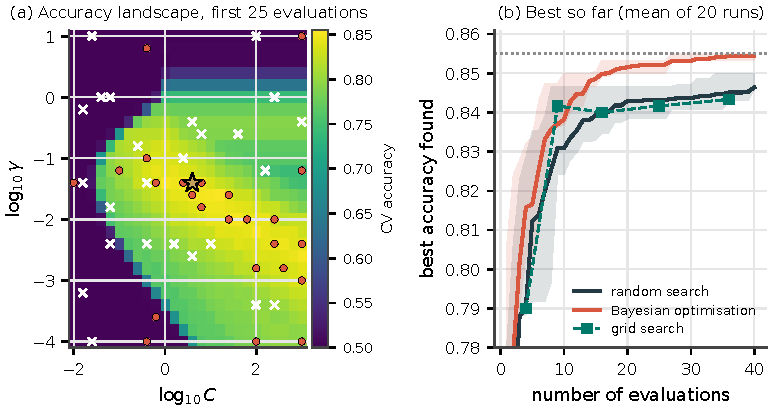
\includegraphics[width=\textwidth]{ch04/hpo_search}
\caption{Hyperparameter optimisation of an RBF SVM. (a) Cross-validation accuracy as a function of
$\log_{10}C$ and $\log_{10}\gamma$, with the first 25 points evaluated by random search (white crosses)
and Bayesian optimisation (red dots) in one run; the star is the optimum. (b) Best accuracy found as a
function of the number of evaluations (mean and interquartile range over 20 runs).}
\label{fig:hpo}
\end{figure}

\subsection{AutoML systems}

Many systems combine these ingredients (\cref{tab:automlsystems}). Auto-WEKA \citep{thornton2013auto}
introduced CASH\index{CASH problem} with Bayesian optimisation\index{Bayesian optimisation} over the algorithms of WEKA. Auto-sklearn
\citep{feurer2015efficient} applies the same idea to scikit-learn and adds two improvements:
metalearning\index{metalearning} to start the search from configurations that worked on similar data sets
(\cref{sec:metalearning}), and an ensemble\index{ensemble} of the models found during the search, built with
ensemble selection \citep{caruana2004ensemble}. TPOT \citep{olson2016evaluation} evolves whole pipelines with
genetic programming\index{genetic programming}. H2O AutoML\index{AutoML} \citep{ledell2020h2o} trains many models with random search\index{random search} and combines
them in stacked ensembles. AutoKeras \citep{jin2019autokeras} searches neural network architectures.
Commercial cloud services offer AutoML with minimal effort, at a price and as a black box.

\begin{table}[htbp]
\centering\small
\caption{Some AutoML systems.}\label{tab:automlsystems}
\begin{tabularx}{\textwidth}{@{}llX@{}}
\toprule
System & Search & Notes\\
\midrule
Auto-WEKA & Bayesian optimisation & the first CASH system, on the WEKA algorithms\\
auto-sklearn & Bayesian optimisation & metalearning warm start; ensemble of the models found\\
TPOT & genetic programming & evolves pipelines of preprocessing and models\\
H2O AutoML & random search & stacked ensembles; Java with Python and R bindings\\
AutoKeras & neural architecture search & based on Keras\\
MLBox, auto\_ml & various & open-source Python libraries\\
\bottomrule
\end{tabularx}
\end{table}

Which system is best? \citet{balaji2018benchmarking} compared auto\_ml, auto-sklearn, TPOT and H2O on 87
OpenML data sets \citep{vanschoren2013openml}, 57 for classification and 30 for regression, with a limit
of three hours per task: auto-sklearn performed best in classification and TPOT in regression. \citet{gijsbers2024amlb}, with a larger
and more recent benchmark, found that no system dominates on every task, and
that the time budget and the data set matter as much as the system.

\subsection{Evaluating AutoML on unseen data}

An AutoML\index{AutoML} system is itself a learning algorithm: it uses data to choose a model. Therefore the
validation score of the configuration it selects is an \emph{optimistic} estimate of its performance,
for the same reason as in \cref{sec:protocols}: among many configurations, the one with the best
validation score owes part of its score to chance. The more configurations are evaluated, the larger the
optimism.

\begin{pylisting}[label={lst:cash}]{Random search over a CASH space: the winner's validation score is optimistic}
import numpy as np
from sklearn.datasets import make_classification
from sklearn.ensemble import RandomForestClassifier
from sklearn.linear_model import LogisticRegression
from sklearn.model_selection import cross_val_score, train_test_split
from sklearn.neighbors import KNeighborsClassifier
from sklearn.pipeline import make_pipeline
from sklearn.preprocessing import StandardScaler
from sklearn.svm import SVC
from sklearn.tree import DecisionTreeClassifier

X, y = make_classification(n_samples=2300, n_features=20, n_informative=5, flip_y=0.1,
                           random_state=5)
X_tr, X_te, y_tr, y_te = train_test_split(X, y, train_size=300, random_state=0)
rng = np.random.default_rng(0)

def random_config(rng):
    """A random point of the CASH space: an algorithm and its hyperparameters."""
    algo = rng.choice(["logistic", "knn", "tree", "forest", "svm"])
    scaled = lambda m: make_pipeline(StandardScaler(), m)
    if algo == "logistic":
        return scaled(LogisticRegression(C=10 ** rng.uniform(-3, 3)))
    if algo == "knn":
        return scaled(KNeighborsClassifier(int(rng.integers(1, 50))))
    if algo == "tree":
        return DecisionTreeClassifier(max_depth=int(rng.integers(1, 20)),
                                      min_samples_leaf=int(rng.integers(1, 20)),
                                      random_state=0)
    if algo == "forest":
        return RandomForestClassifier(int(rng.integers(10, 200)),
                                      max_features=float(rng.uniform(0.1, 1)),
                                      random_state=0)
    return scaled(SVC(C=10 ** rng.uniform(-2, 3), gamma=10 ** rng.uniform(-4, 1)))

configs = [random_config(rng) for _ in range(200)]
cv = np.array([cross_val_score(c, X_tr, y_tr, cv=5).mean() for c in configs])
test = np.array([c.fit(X_tr, y_tr).score(X_te, y_te) for c in configs])
print("budget  best CV accuracy  test accuracy of that configuration")
for B in (1, 5, 20, 50, 100, 200):          # random search with budget B
    picks = [rng.choice(200, B, replace=False) for _ in range(500)]
    best = [idx[np.argmax(cv[idx])] for idx in picks]
    print(f"{B:5d}       {cv[best].mean():.3f}              {test[best].mean():.3f}")
print(f"best test accuracy of any configuration: {test.max():.3f}")
\end{pylisting}
\begin{pyoutput}
budget  best CV accuracy  test accuracy of that configuration
    1       0.839              0.837
    5       0.914              0.904
   20       0.930              0.911
   50       0.938              0.917
  100       0.945              0.922
  200       0.950              0.925
best test accuracy of any configuration: 0.928
\end{pyoutput}

\Cref{lst:cash} and \cref{fig:optimism} make the effect visible. Two hundred random configurations of
five algorithms (logistic regression\index{logistic regression}, $k$-nearest neighbours\index{k-nearest neighbours@$k$-nearest neighbours}, decision trees\index{decision tree}, random forests and SVMs,
with their hyperparameters) are evaluated with 5-fold cross-validation on 300 training examples, and
on 2000 test examples that the search never sees. As the budget grows, the cross-validation accuracy of
the winner rises from 0.839 to 0.950, but its test accuracy only from 0.837 to 0.925: with 200
configurations the optimism is 2.5 points. The search is still useful (the selected configuration is
close to the best one, 0.928), but its own score must not be reported as the expected performance. The
remedy is the one of \cref{sec:protocols}: evaluate the whole AutoML process, including the search, on
data it has not used, with a separate test set\index{test set} or nested cross-validation\index{cross-validation!nested}.

\begin{figure}[htbp]
\centering
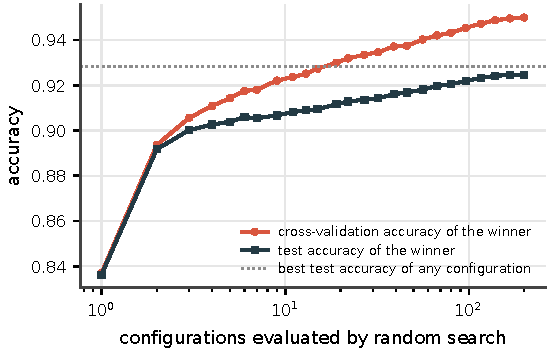
\includegraphics[width=0.7\textwidth]{ch04/automl_optimism}
\caption{Random search over a CASH space: cross-validation accuracy of the selected configuration
and its accuracy on new data, as a function of the number of configurations evaluated (mean over 500
repetitions).}
\label{fig:optimism}
\end{figure}

% =====================================================================
\section{Metalearning}\label{sec:metalearning}

\emph{Metalearning\index{metalearning|textbf}} applies learning algorithms to metadata about machine learning experiments, to
understand how learning can become flexible and, ultimately, to learn the learning process itself:
\emph{learning to learn} \citep{brazdil2022metalearning,vanschoren2018meta}. Within machine learning
the term also covers algorithms that learn from the outputs of other algorithms, such as the
meta-learner of stacking\index{stacking} (\cref{sec:hybrid}).

The classical formulation is the \emph{algorithm selection\index{algorithm selection|textbf} problem} \citep{rice1976algorithm}: given a
new data set, which algorithm will perform best on it? Each data set from previous experiments is
described by \emph{meta-features}, and a \emph{meta-model} learns to map them to the best algorithm (or
to the expected performance of each one). Meta-features can be simple (number of examples, features
and classes), statistical (correlations, skewness, class imbalance\index{class imbalance}), information-theoretic (class
entropy, mutual information) or \emph{landmarkers\index{landmarker|textbf}}, the performance of fast, simple algorithms such as
a decision stump\index{decision stump} or a linear discriminant \citep{pfahringer2000meta}. Metalearning is used to recommend
algorithms, to start the hyperparameter search of AutoML\index{AutoML} systems from configurations that worked on
similar data sets, and, in deep learning, to train models that adapt quickly to new tasks from a few
examples \citep{finn2017model}.

\begin{pylisting}[label={lst:meta}]{Algorithm selection with meta-features and landmarkers}
import numpy as np
from sklearn.datasets import make_classification
from sklearn.discriminant_analysis import LinearDiscriminantAnalysis
from sklearn.ensemble import RandomForestClassifier
from sklearn.linear_model import LogisticRegression
from sklearn.model_selection import LeaveOneOut, cross_val_predict, cross_val_score
from sklearn.neighbors import KNeighborsClassifier
from sklearn.pipeline import make_pipeline
from sklearn.preprocessing import StandardScaler
from sklearn.tree import DecisionTreeClassifier, export_text

rng = np.random.default_rng(0)
LR = make_pipeline(StandardScaler(), LogisticRegression(max_iter=2000))
RF = RandomForestClassifier(100, random_state=0, n_jobs=-1)

def random_task(rng):
    """A random binary classification data set with varied size, noise and shape."""
    n, d = int(rng.integers(100, 600)), int(rng.integers(2, 40))
    inf = int(min(d, rng.integers(2, 6)))
    clusters = int(min(rng.integers(1, 4), 2 ** inf // 2))
    return make_classification(n_samples=n, n_features=d, n_informative=inf,
                               n_redundant=0, n_clusters_per_class=clusters,
                               class_sep=rng.uniform(0.5, 2), flip_y=rng.uniform(0, 0.1),
                               random_state=int(rng.integers(1e6)))

def meta_features(X, y):
    """Simple, statistical and landmarking meta-features (Pfahringer et al., 2000)."""
    n, d = X.shape
    land = lambda m: cross_val_score(m, X, y, cv=3).mean()
    return [np.log10(n), np.log10(d), np.log10(n / d), min(y.mean(), 1 - y.mean()),
            land(LinearDiscriminantAnalysis()), land(DecisionTreeClassifier(max_depth=1)),
            land(make_pipeline(StandardScaler(), KNeighborsClassifier(1)))]

NAMES = ["log_n", "log_d", "log_n/d", "minority", "lm_linear", "lm_stump", "lm_1nn"]
tasks = [random_task(rng) for _ in range(120)]
M = np.array([meta_features(X, y) for X, y in tasks])
acc = np.array([[cross_val_score(m, X, y, cv=3).mean() for m in (LR, RF)]
                for X, y in tasks])
winner = (acc[:, 1] > acc[:, 0]).astype(int)                 # 1 if the forest is better
meta = DecisionTreeClassifier(max_depth=2, random_state=0)
# leave one task out: the meta-model never sees the task it chooses an algorithm for
choice = cross_val_predict(meta, M, winner, cv=LeaveOneOut())
chosen = acc[np.arange(len(acc)), choice]
print(f"the forest wins on {winner.mean():.0%} of the 120 tasks")
print(f"meta-model picks the better algorithm on {np.mean(choice == winner):.0%} of them")
print(f"it chooses the logistic regression for {np.sum(choice == 0)} tasks")
for name, a in [("always logistic", acc[:, 0]), ("always forest", acc[:, 1]),
                ("meta-learned choice", chosen), ("oracle", acc.max(axis=1))]:
    regret = acc.max(axis=1) - a                  # accuracy lost against the best choice
    print(f"{name:20s} mean accuracy {a.mean():.4f}   mean regret {regret.mean():.4f}"
          f"   worst regret {regret.max():.3f}")
print(export_text(meta.fit(M, winner), feature_names=NAMES), end="")
\end{pylisting}
\begin{pyoutput}
the forest wins on 74% of the 120 tasks
meta-model picks the better algorithm on 81% of them
it chooses the logistic regression for 16 tasks
always logistic      mean accuracy 0.8253   mean regret 0.0393   worst regret 0.290
always forest        mean accuracy 0.8613   mean regret 0.0034   worst regret 0.076
meta-learned choice  mean accuracy 0.8613   mean regret 0.0033   worst regret 0.076
oracle               mean accuracy 0.8646   mean regret 0.0000   worst regret 0.000
|--- lm_linear <= 0.93
|   |--- lm_linear <= 0.82
|   |   |--- class: 1
|   |--- lm_linear >  0.82
|   |   |--- class: 1
|--- lm_linear >  0.93
|   |--- log_d <= 1.41
|   |   |--- class: 0
|   |--- log_d >  1.41
|   |   |--- class: 1
\end{pyoutput}

\Cref{lst:meta} and \cref{fig:meta} build a small metalearning system. On 120 random classification
tasks of different sizes, dimensions and shapes, we compute seven meta-features and the
cross-validation accuracy of a logistic regression and a random forest, and train a depth-2 tree to
predict which one is better, evaluating it by leaving one task out at a time. The forest wins on 74\%
of the tasks; the meta-model picks the better algorithm on 81\%, and the rule it learns is readable:
choose the logistic regression when a linear discriminant already reaches an accuracy above 0.93 and
there are at most 25 features, and the forest otherwise.

\begin{figure}[htbp]
\centering
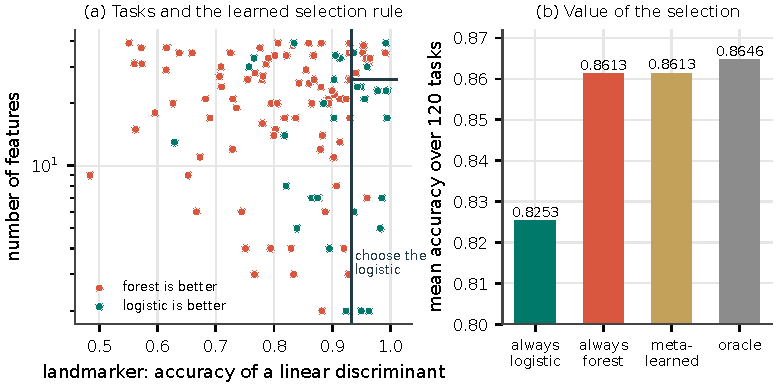
\includegraphics[width=\textwidth]{ch04/metalearning}
\caption{Algorithm selection on 120 tasks. (a) Each point is a task, coloured by the better algorithm;
the lines are the rule learned by the meta-model. (b) Mean accuracy of always choosing one algorithm, of
the meta-learned choice and of an oracle that always knows the better one.}
\label{fig:meta}
\end{figure}

Yet the mean accuracy of the meta-learned choice (0.8613) is the same as that of always choosing the
forest. The reason is that the forest is rarely much worse than the logistic regression (its
mean \emph{regret\index{regret|textbf}}, the accuracy lost against the better algorithm, is 0.0034), so even an oracle could
only gain 0.0033 on average, and the cases the meta-model gets right are those where the difference is
smallest. What the meta-model does achieve is to choose the simpler, more interpretable\index{interpretability} model on 16
tasks at no cost in \emph{mean} accuracy (the logistic regression is worse than the forest on some of
those tasks and better on others). Note also what is being measured: leave-one-task-out tests how well
the meta-model predicts the cross-validation winner of an unseen task; evaluating the whole selection
procedure on new data would require computing the landmarkers on each task's training data and testing
the chosen learner on separate data within the task. Before investing in algorithm selection, measure how much the oracle
could gain: metalearning helps when the candidate algorithms are complementary. It helps little when one of them
is almost always good enough, a situation that the benchmarks of \cref{sec:performance} show is common
for tabular data.

% =====================================================================
\section{Inductive programming\extsec}\label{sec:indprog}

\emph{Inductive programming\index{inductive programming|textbf}} (IP) is an interdisciplinary area of artificial intelligence and
cognitive science that studies the automatic synthesis of computer programs from examples and
background knowledge\index{background knowledge}, typically a set of existing functions
\citep{kitzelmann2009inductive,gulwani2015inductive}. Like all inductive inference, it generalises from
observations by identifying general patterns, but the hypotheses it produces are programs, which are
expressive, recursive if needed, and readable. IP is usually addressed from two perspectives:
\emph{inductive logic programming\index{inductive logic programming|textbf}}, in the logic paradigm, and \emph{inductive functional programming\index{inductive functional programming|textbf}},
in the functional paradigm. \emph{Programming by example\index{programming by example|textbf}} (PbE) is the part of IP in which the
specification is a set of input--output examples, and it can automate many data manipulation tasks:
extracting terms from texts, transforming data formats, and so on.

\subsection{Inductive logic programming}

Inductive logic programming\index{inductive logic programming} (ILP) uses logic programs as a uniform representation for the examples,
the background knowledge\index{background knowledge} and the hypotheses \citep{muggleton1991inductive,muggleton1994inductive}. Given
positive examples $E^+$, negative examples $E^-$ and background knowledge $B$, an ILP system derives a
hypothesis $H$, a logic program, that together with $B$ entails all the positive examples and none of
the negative ones:
\begin{equation}
  B\wedge H\models E^+,\qquad B\wedge H\not\models e\ \text{ for every } e\in E^- .
\end{equation}
For example, with the background knowledge \texttt{parent(a,b)}, \texttt{parent(a,c)},
\texttt{parent(d,b)}, \texttt{male(a)}, \texttt{female(c)}, \texttt{female(d)} and the positive examples
\texttt{father(a,b)}, \texttt{father(a,c)}, an ILP system induces
\begin{center}
\texttt{father(X,Y) :- parent(X,Y), male(X).}
\end{center}
\Cref{lst:ilp} implements the simplest possible ILP system: it enumerates clause bodies of increasing
length built from the background predicates, and returns the first one that covers every positive and
no negative example (under the closed-world assumption, every pair not listed as positive is
negative). It finds the definitions of \texttt{father} and \texttt{mother}, and, on a larger family,
\texttt{grandparent(X,Y) :- parent(X,Z), parent(Z,Y)}, which needs a new variable $Z$ that does not
appear in the head. Real systems, such as FOIL \citep{quinlan1990learning}, search this space much more
cleverly, because it grows very fast: even our 12 candidate literals give 78 bodies of length at most
two.

\begin{pylisting}[label={lst:ilp}]{A brute-force inductive logic programming system}
from itertools import combinations, product

# Candidate body literals over the head variables X, Y and an extra variable Z
LITERALS = [("parent", v) for v in product("XYZ", repeat=2) if v[0] != v[1]] + \
           [(p, (v,)) for p in ("male", "female") for v in "XYZ"]

def covers(body, x, y, B, people):
    """Does the body entail the head p(x, y) for some value of Z?"""
    return any(all(tuple({"X": x, "Y": y, "Z": z}[v] for v in args) in B[pred]
                   for pred, args in body) for z in people)

def learn(positives, B):
    """Shortest body that covers all positives and no negative (closed world)."""
    people = sorted({c for facts in B.values() for f in facts for c in f})
    negatives = [(x, y) for x in people for y in people if (x, y) not in positives]
    for size in (1, 2):
        for body in combinations(LITERALS, size):
            if all(covers(body, *e, B, people) for e in positives) and \
               not any(covers(body, *e, B, people) for e in negatives):
                return body

show = lambda head, body: f"{head}(X,Y) :- " + ", ".join(
    f"{p}({','.join(a)})" for p, a in body)
B = {"parent": {("a", "b"), ("a", "c"), ("d", "b")},              # background knowledge
     "male": {("a",)}, "female": {("c",), ("d",)}}
print(show("father", learn({("a", "b"), ("a", "c")}, B)))
print(show("mother", learn({("d", "b")}, B)))
B2 = {"parent": {("ann", "bob"), ("bob", "carl"), ("bob", "dora"), ("eve", "fred"),
                 ("fred", "gina"), ("eve", "hugo")}, "male": set(), "female": set()}
print(show("grandparent", learn({("ann", "carl"), ("ann", "dora"), ("eve", "gina")}, B2)))
n_bodies = len(LITERALS) * (len(LITERALS) + 1) // 2
print(f"{len(LITERALS)} literals: {n_bodies} bodies of size <= 2")
\end{pylisting}
\begin{pyoutput}
father(X,Y) :- parent(X,Y), male(X)
mother(X,Y) :- parent(X,Y), female(X)
grandparent(X,Y) :- parent(X,Z), parent(Z,Y)
12 literals: 78 bodies of size <= 2
\end{pyoutput}

ILP can learn from structured examples that do not fit in a table. In Michalski's classic trains problem
\citep{michalski1980pattern}, each train is a list of cars, each car has a shape, a length, a roof, a
number of wheels and a load, and the task is to tell trains travelling east from trains travelling
west. Represented as a logic program, an eastbound train is the fact
\begin{center}\small
\texttt{eastbound([car(rect,short,none,2,load(circ,1)), car(rect,long,none,3,load(hexa,1)),}\\
\texttt{car(rect,short,peak,2,load(tria,1)), car(rect,long,none,2,load(rect,3))]).}
\end{center}
With the background predicates \texttt{member}, \texttt{arg} and \texttt{not}, an ILP system induces
\begin{center}
\texttt{eastbound(T) :- member(C,T), arg(2,C,short), not arg(3,C,none).}
\end{center}
that is, a train goes east if it has a short car with a roof.

\subsection{Inductive functional programming}

Inductive functional programming\index{inductive functional programming} (IFP) expresses knowledge as functions. In the trains problem, a train
becomes a list of tuples, \texttt{type Train = [Car]} with \texttt{type Car = (Shape, Length, Roof,
Wheels, Load)}, and the target is a function \texttt{eastbound :: Train -> Bool} specified by examples
such as \texttt{eastbound [(Rect, Short, Peak, 2, (Tria, 1)), \dots] = True}. Systems such as
MagicHaskeller \citep{katayama2008efficient} search the space of functional programs built from a library
of background functions, in order of increasing size, and return the first ones consistent with the
examples.

\Cref{lst:ifp} does the same for a tiny problem, a number sequence given by the examples $6\mapsto14$,
$3\mapsto8$, $5\mapsto12$ and $2\mapsto6$. With the background knowledge\index{background knowledge} $\{x,1,2,+,\times\}$ it
enumerates programs by the number of functions they use. No program with zero or one function fits;
among the 216 programs with two functions, 14 are consistent with the examples, such as
$x+(x+2)$ or, written differently, $2(x+1)$, and all of them predict 10 for the input 4. The listing also
shows how fast the space grows: 3, 18, 216, 3240 and 54,432 programs with 0 to 4 functions. Many of the
programs are equivalent, and practical systems avoid generating programs that behave identically on
the examples.

\begin{pylisting}[label={lst:ifp}]{Enumerating functional programs by size}
from functools import lru_cache
from itertools import product

LEAVES, FUNCTIONS = ("x", "1", "2"), ("+", "*")           # the background knowledge

@lru_cache(maxsize=None)
def programs(k):
    """All expressions with exactly k functions, as fully parenthesised strings."""
    if k == 0:
        return LEAVES
    return tuple(f"({a} {f} {b})" for left in range(k)
                 for a, b, f in product(programs(left), programs(k - 1 - left),
                                        FUNCTIONS))

examples = [(6, 14), (3, 8), (5, 12), (2, 6)]               # input -> output
print("programs with 0..4 functions:", [len(programs(k)) for k in range(5)])
for k in range(5):
    hits = [p for p in programs(k) if all(eval(p, {"x": x}) == y for x, y in examples)]
    if hits:
        break
evaluated = sum(len(programs(j)) for j in range(k + 1))
print(f"{len(hits)} consistent programs with {k} functions "
      f"({evaluated} programs evaluated)")
print("e.g.", ", ".join(hits[:3]))
print("for input 4 they output", eval(hits[0], {"x": 4}))
\end{pylisting}
\begin{pyoutput}
programs with 0..4 functions: [3, 18, 216, 3240, 54432]
14 consistent programs with 2 functions (237 programs evaluated)
e.g. (x + (x + 2)), (x + (2 + x)), (2 + (x + x))
for input 4 they output 10
\end{pyoutput}

\subsection{Inductive bias}

The choice of the functions in the background knowledge\index{background knowledge} is a form of \emph{inductive bias\index{inductive bias|textbf}}, the set of
assumptions a learning system makes to prefer some hypotheses over others. How many candidate programs there are
depends on the grammar. A sequence of $d$ choices among $b$ functions has $b^d$ possibilities. The ordered binary expressions with $k$ operator nodes, $b$ binary operators and $l$ terminals number
$C_k\,b^k\,l^{k+1}$, where the Catalan number $C_k=\binom{2k}{k}/(k+1)$ counts the shapes of the tree; with two
operators and three terminals, this gives the 3, 18, 216, 3240 and 54,432 expressions of \cref{lst:ifp}.
Either way, the space grows exponentially with the size of the programs. Two kinds of bias keep the search tractable:
\begin{itemize}
  \item \emph{language bias\index{language bias|textbf}} restricts the hypothesis space, that is, which programs can be induced (the
        background functions, the maximum length, the types);
  \item \emph{search bias} determines how the space is explored, that is, which programs are
        constructed first (by size, by a probability distribution, by a heuristic).
\end{itemize}
Choosing the background knowledge dynamically for each problem, from a large library, is one way of
getting the right bias for each task \citep{contrerasochando2019automated,contrerasochando2021towards}.

\subsection{Programming by example and domain-specific languages}

\emph{Domain-specific languages\index{domain-specific language|textbf}} (DSLs) are languages specialised for a particular domain, such as
string processing or number formatting. Inducing programs in a small DSL reduces the search space
considerably, which is what made inductive programming\index{inductive programming} practical for end users. Flash Fill\index{Flash Fill} in Excel
\citep{gulwani2011automating} induces string transformations in a DSL of substrings, positions and
concatenations from one or two examples typed in a spreadsheet, and similar features appear in other
spreadsheets and programming environments. Inductive programming can automate tedious tasks in many other domains.

\begin{pylisting}[label={lst:pbe}]{Programming by example with a small string DSL}
import re

TOKENS = {"word": r"[A-Za-z]+", "number": r"\d+"}
# positions: first, second, third, last and penultimate token
INDEXES = (0, 1, 2, -1, -2)

def atoms(inp, piece):
    """The atoms of the DSL that produce the string `piece` from the input `inp`."""
    found = []
    for kind, rx in TOKENS.items():
        toks = re.findall(rx, inp)
        found += [("token", kind, k) for k in INDEXES
                  if -len(toks) <= k < len(toks) and toks[k] == piece]
    words = re.findall(TOKENS["word"], inp)
    if len(piece) == 1:
        found += [("initial", "word", k) for k in INDEXES
                  if -len(words) <= k < len(words) and words[k][0] == piece]
    if len(piece) <= 2 and not any(ch.isalnum() for ch in piece):
        found.append(("const", piece))            # language bias: short separators only
    return found

def run(program, inp):
    out = ""
    for kind, *arg in program:
        if kind == "const":
            out += arg[0]
            continue
        toks = re.findall(TOKENS[arg[0]], inp)
        if not -len(toks) <= arg[1] < len(toks):
            return None
        out += toks[arg[1]] if kind == "token" else toks[arg[1]][0]
    return out

def consistent(inp, out):
    """Every program (sequence of atoms) that maps inp to out."""
    if not out:
        return [()]
    return [(a,) + rest for i in range(1, len(out) + 1)
            for a in atoms(inp, out[:i]) for rest in consistent(inp, out[i:])]

def learn(examples):
    progs = [p for p in consistent(*examples[0])
             if all(run(p, i) == o for i, o in examples[1:])]
    return sorted(progs, key=lambda p: (len(p), sum(a[0] == "const" for a in p)))

show = lambda p: " + ".join(f'"{a[1]}"' if a[0] == "const" else f"{a[0]}({a[1]},{a[2]})"
                            for a in p)
tasks = {"first name": ([("Cesar Ferri", "Cesar"), ("Ana Gil", "Ana")],
                        ["Pau Torres", "Maria Jose Ramirez"]),
         "US date": ([("23/12/2021", "12-23-2021")], ["05/01/2022"]),
         "initials": ([("Cesar Ferri", "C.F."), ("Ana Gil", "A.G.")], ["Juan Garcia"]),
         "domain": ([("ana.gil@upv.es", "upv.es")], ["cferri@dsic.upv.es"])}
for name, (examples, tests) in tasks.items():
    progs = learn(examples)
    outs = {t: sorted({run(p, t) for p in progs}) for t in tests}
    print(f"{name}: {len(progs)} consistent programs")
    print(f"    best: {show(progs[0])}")
    for t, o in outs.items():
        print(f"    {t} -> {run(progs[0], t)}   (all consistent programs: {o})")
\end{pylisting}
\begin{pyoutput}
first name: 2 consistent programs
    best: token(word,0)
    Pau Torres -> Pau   (all consistent programs: ['Pau'])
    Maria Jose Ramirez -> Maria   (all consistent programs: ['Jose', 'Maria'])
US date: 4 consistent programs
    best: token(number,1) + "-" + token(number,0) + "-" + token(number,2)
    05/01/2022 -> 01-05-2022   (all consistent programs: ['01-05-2022'])
initials: 4 consistent programs
    best: initial(word,0) + "." + initial(word,1) + "."
    Juan Garcia -> J.G.   (all consistent programs: ['J.G.'])
domain: 2 consistent programs
    best: token(word,2) + "." + token(word,-1)
    cferri@dsic.upv.es -> upv.es   (all consistent programs: ['upv.es'])
\end{pyoutput}

\Cref{lst:pbe} implements a minimal Flash Fill. A program is a concatenation of \emph{atoms}: the
$k$-th word or number of the input ($k=0,1,2$ or the last or penultimate), the initial of a word, or a
short constant separator. For each example, the system enumerates every way of producing the output as
a concatenation of atoms, keeps the programs consistent with all the examples, and prefers the shortest
ones. From two examples it learns to extract first names, from one example to turn a date into the US
format, and from two examples to build initials. The listing also exposes the two classical problems of
PbE:
\begin{itemize}
  \item \emph{ambiguity}: several programs fit the examples and disagree on new inputs. For the first
        names, ``the first word'' and ``the penultimate word'' fit both examples, and give different
        answers for a person with two first names, such as \texttt{Maria Jose Ramirez};
  \item \emph{language bias\index{language bias|textbf}}: the domain of \texttt{ana.gil@upv.es} is learned as the penultimate and
        last words, so \texttt{cferri@dsic.upv.es} becomes \texttt{upv.es}, because the DSL cannot express
        ``everything after the @''. A language that is too permissive also causes errors: in a first version of the listing,
        constants could contain digits, and the shortest program for the date hard-coded \texttt{"-2"}
        and \texttt{"3-"}, turning \texttt{05/01/2022} into \texttt{01-23-2022}.
\end{itemize}
Practical systems address ambiguity by ranking programs with learned preferences and by showing the
user the inputs on which the candidate programs disagree, so that one more example resolves the
doubt.

\subsection{Language models as inductive programmers}

\emph{Language models\index{language model|textbf}} estimate the probability $p(y\mid x)$ of a sequence of characters or words $y$
following another sequence $x$. Built with large attention-based (transformer) architectures
\citep{vaswani2017attention} and trained on huge amounts of text and code, systems such as GPT-3 turned
out to be \emph{few-shot learners} \citep{brown2020language}: given a prompt\index{prompt} with a few examples, they
continue the pattern. They can extrapolate from short prompts in mathematical
problem solving, question answering, language understanding and code generation
\citep{chen2021evaluating}.

They can therefore be used for data wrangling\index{data wrangling} \citep{jaimovitch2023can}. They infer transformations
from very few examples, as in the prompt
\begin{center}
\texttt{input: 23/12/2021, output: 12-23-2021 \quad input: 05/01/2022, output:}
\end{center}
and they bring a wide range of background knowledge\index{background knowledge} without being told: we do not need to say that
\texttt{23/12/2021} is a date, or that \texttt{Cesar Ferri} is a person's name whose first word is the
first name. Hints in the prompt make few-shot learning more effective, and even \emph{zero-shot}
learning is possible: ``The conversion of 23/12/2021 into US format is:''. A prompt such as
\texttt{input: 6, output: 14, input: 3, output: 8, input: 5, output: 12, input: 2, output: 6, input: 4,
output:} poses the problem of \cref{lst:ifp} without any background functions. These prompts ask for
output values; a language model can also be asked to write the
transformation as code, which can be inspected and tested (\cref{sec:llmds}). In both modes its answers
can be plausible and wrong;
as with any inductive method, the outputs must be checked, for instance on held-out examples, before
the transformation is applied to a whole data set. \Cref{sec:llmds} looks at what language models can
do for the rest of the data science process.

% =====================================================================
\section{Genetic programming\extsec}\label{sec:gp}

\emph{Genetic programming\index{genetic programming|textbf}} (GP) evolves computer programs \citep{koza1992genetic,poli2008field}. Inspired
by natural evolution, it is a heuristic search for an optimal, or at least suitable, program in the
space of all programs, starting from a random population of programs and applying three operations:
\begin{itemize}
  \item \emph{selection}: individuals are chosen to reproduce probabilistically, so that better programs
        have a higher chance of being selected (for instance, by \emph{tournament}: the best of a few
        individuals taken at random);
  \item \emph{crossover\index{genetic programming!crossover|textbf}}: two selected programs are combined, typically by replacing a random part of
        one of them by a random part of the other;
  \item \emph{mutation\index{genetic programming!mutation|textbf}}: a random part of a program is replaced by a new random part.
\end{itemize}
The rates at which these operators are applied determine the diversity\index{genetic programming!diversity} of the population. The idea is
old: Alan Turing already suggested, in 1950, that a learning machine could be found by a process
analogous to evolution \citep{turing1950computing}.

Programs are traditionally represented as trees, in which every internal node is a function and every
leaf an operand (a variable or a constant), which makes them easy to evolve and evaluate
(\cref{fig:gptrees}).

\begin{figure}[htbp]
\centering
\begin{tikzpicture}[font=\small\sffamily,
  every node/.style={circle,draw=edmnavy,fill=edmnavy!6,minimum size=6.5mm,inner sep=0pt},
  hl/.style={fill=edmcoral!25,draw=edmcoral},
  level distance=10mm,
  level 1/.style={sibling distance=15mm},
  level 2/.style={sibling distance=8mm},
  edge from parent/.style={draw=edmnavy}]
  \node at (0,0) {$+$}
    child {node {$\times$} child {node {$x$}} child {node {$x$}}}
    child {node[hl] {$y$}};
  \node[draw=none,fill=none,rectangle] at (0,-3.0) {parent 1: $x^2+y$};
  \begin{scope}[xshift=4.8cm]
  \node[hl] at (0,0) {$-$}
    child[edge from parent/.style={draw=edmcoral}] {node[hl] {$\times$} child {node[hl] {$x$}} child {node[hl] {$y$}}}
    child[edge from parent/.style={draw=edmcoral}] {node[hl] {$3$}};
  \node[draw=none,fill=none,rectangle] at (0,-3.0) {parent 2: $xy-3$};
  \end{scope}
  \begin{scope}[xshift=10cm, level 1/.style={sibling distance=17mm}]
  \node at (0,0) {$+$}
    child {node {$\times$} child {node {$x$}} child {node {$x$}}}
    child {node[hl] {$-$}
      child {node[hl] {$\times$} child {node[hl] {$x$}} child {node[hl] {$y$}}}
      child {node[hl] {$3$}}};
  \node[draw=none,fill=none,rectangle] at (0,-3.9) {child: $x^2+xy-3$};
  \end{scope}
\end{tikzpicture}
\caption{Programs as trees and subtree crossover: the subtree $y$ of the first parent is replaced by the
whole second parent (or any of its subtrees), producing a child that neither parent represents.}
\label{fig:gptrees}
\end{figure}

\begin{algorithm}[htbp]
\caption{Genetic programming.}\label{alg:gp}
\begin{algorithmic}[1]
\State create an initial random population of programs
\Repeat
  \State evaluate every program with the fitness function and rank them
  \State pass the best program unchanged to the next generation \Comment{elitism}
  \State build the rest of the next generation by selecting good programs and applying crossover
         and mutation
\Until{a program has a perfect score or a stopping criterion (e.g.\ a number of generations) is met}
\State \Return the best program
\end{algorithmic}
\end{algorithm}

\Cref{alg:gp} summarises the method. \Cref{lst:gp} applies it to \emph{symbolic regression\index{symbolic regression|textbf}}: from 200
points of a hidden function of two variables, find a formula for it. The functions are $+$, $-$ and
$\times$, the terminals $x$, $y$, 1, 2 and 3, the fitness\index{genetic programming!fitness} is the mean squared error\index{mean squared error (MSE)}, and the population
has 300 programs, with tournament selection, subtree crossover, occasional mutation, elitism\index{genetic programming!elitism} and a
maximum depth to limit \emph{bloat} (the tendency of programs to grow without improving). In generation
11 the best program, $((y\cdot2+(x-y))\cdot x)-3$, has zero error; simplified, it is exactly the hidden
function $x^2+xy-3$ (\cref{fig:gpevo}). Evolution proceeds by jumps: the best error stays at 4.0 from generation 2 to generation 10,
and then drops to zero when a crossover combines the right building blocks.

\begin{pylisting}[label={lst:gp}]{Genetic programming for symbolic regression, from scratch}
import random
import numpy as np
import sympy

rng = random.Random(3)
x, y = np.random.default_rng(0).uniform(-3, 3, (2, 200))
target = x * x + x * y - 3                        # the hidden function to rediscover
OPS = {"+": np.add, "-": np.subtract, "*": np.multiply}
TERMINALS = ["x", "y", 1, 2, 3]

def random_tree(depth):
    if depth == 0 or rng.random() < 0.3:
        return rng.choice(TERMINALS)
    return (rng.choice(list(OPS)), random_tree(depth - 1), random_tree(depth - 1))

def evaluate(t):
    if isinstance(t, tuple):
        return OPS[t[0]](evaluate(t[1]), evaluate(t[2]))
    return x if t == "x" else y if t == "y" else np.full_like(x, t)

def error(t):
    return float(np.mean((evaluate(t) - target) ** 2))

def paths(t, path=()):                            # positions of all the subtrees
    yield path
    if isinstance(t, tuple):
        yield from paths(t[1], path + (1,))
        yield from paths(t[2], path + (2,))

def get(t, path):
    for i in path:
        t = t[i]
    return t

def put(t, path, new):
    if not path:
        return new
    return tuple(put(s, path[1:], new) if i == path[0] else s for i, s in enumerate(t))

def depth(t):
    return 1 + max(depth(t[1]), depth(t[2])) if isinstance(t, tuple) else 0

def crossover(a, b):                              # a subtree of b replaces one of a
    return put(a, rng.choice(list(paths(a))), get(b, rng.choice(list(paths(b)))))

def mutate(t):                                    # a random subtree becomes a new one
    return put(t, rng.choice(list(paths(t))), random_tree(2))

def tournament(errs, k=3):
    return min(rng.sample(range(len(errs)), k), key=lambda i: errs[i])

MAX_GEN = 60
pop, history = [random_tree(4) for _ in range(300)], []
for gen in range(MAX_GEN):
    errs = [error(t) for t in pop]
    best = min(range(len(pop)), key=errs.__getitem__)
    history.append((errs[best], float(np.median(errs))))
    if gen % 10 == 0 or errs[best] < 1e-12:
        print(f"generation {gen:2d}: best error {errs[best]:9.4f}, "
              f"median {history[-1][1]:9.1f}")
    if errs[best] < 1e-12 or gen == MAX_GEN - 1:
        break                          # pop[best] belongs to the evaluated population
    children = [pop[best]]                                        # elitism
    while len(children) < len(pop):
        child = crossover(pop[tournament(errs)], pop[tournament(errs)])
        if rng.random() < 0.2:
            child = mutate(child)
        if depth(child) <= 8:                                      # limit bloat
            children.append(child)
    pop = children
show = lambda t: f"({show(t[1])} {t[0]} {show(t[2])})" if isinstance(t, tuple) else str(t)
print("program:   ", show(pop[best]))
print("simplified:", sympy.expand(sympy.sympify(show(pop[best]))))
\end{pylisting}
\begin{pyoutput}
generation  0: best error    8.3611, median      31.7
generation 10: best error    4.0000, median      17.8
generation 11: best error    0.0000, median      17.8
program:    ((((y * 2) + (x - y)) * x) - 3)
simplified: x**2 + x*y - 3
\end{pyoutput}

\begin{figure}[htbp]
\centering
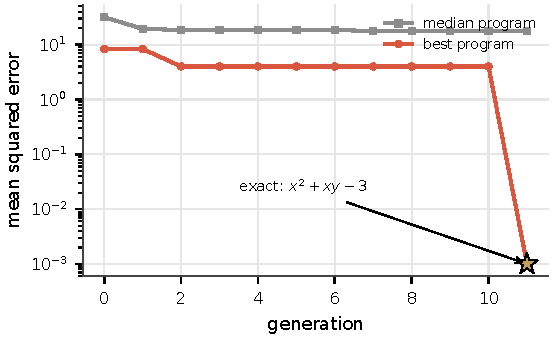
\includegraphics[width=0.7\textwidth]{ch04/gp_evolution}
\caption{Error of the best and the median program of each generation in \cref{lst:gp}.}
\label{fig:gpevo}
\end{figure}

GP has been used for automatic programming and code generation, symbolic regression (including the
rediscovery of physical laws from data, \citealp{schmidt2009distilling}), feature selection and
construction, the design of antennas that flew on a NASA mission \citep{hornby2006automated}, photonic
crystals, optical and quantum computing systems and other inventions, and to play games such as chess,
backgammon and video games. It also powers AutoML\index{AutoML} systems such as TPOT, whose individuals are whole
pipelines. Its weaknesses are the cost of evaluating many programs, the bloat of the evolved programs,
which often need simplification to be readable, and overfitting, since a flexible enough program can fit
the noise in the data: the protocols of \cref{sec:protocols} apply to evolved programs as to any other
model.

% =====================================================================
\section{Large language models for data science}\label{sec:llmds}

The language models of \cref{sec:indprog} can do more than continue a pattern of examples. Trained on huge
amounts of text and code, and then tuned to follow instructions, they became general-purpose assistants that
write programs in Python or SQL from a description in natural language, know the conventions of the main
libraries, explain code and results, and are now built into notebooks and development environments. For data
science, the main change is in the interface: what used to require knowing pandas or scikit-learn
can be asked for in a sentence, a step further in the direction of programming by example\index{programming by example} (\cref{sec:indprog}).
Two questions follow: which parts of the data science process do they automate, and how can the results be
trusted?

\subsection{Assistants along the data science trajectory}

\Cref{tab:llmstages} revisits the stages of \cref{tab:automation} from the point of view of a language model
assistant \citep{debie2022automating,tornede2024automl}. Assistants can help at every stage, including the ones
that classical automation does not reach, such as drafting the questions for a first meeting with a client.
But at every stage they can also fail, and the most dangerous failures are those that do not raise an error.

\begin{table}[htbp]
\centering\small
\caption{What a language model assistant can do at each stage of a project, and what can go wrong.}\label{tab:llmstages}
\begin{tabularx}{\textwidth}{@{}>{\raggedright\arraybackslash}p{2.4cm}>{\raggedright\arraybackslash}X>{\raggedright\arraybackslash}X@{}}
\toprule
Stage & What an assistant can do & What can go wrong\\
\midrule
Problem analysis & draft questions for the client; turn a business goal into candidate targets and metrics;
summarise documents & plausible but generic framing: it does not know the organisation\\
Data understanding & describe the columns, guess their semantic types (dates, currencies, identifiers),
summarise a data set & confident interpretations of ambiguous fields\\
Data preparation & write wrangling and cleaning code from a description or a few examples; match entities,
impute values, detect errors \citep{narayan2022can,jaimovitch2023can} & code that runs but silently drops,
duplicates or misaligns rows\\
Feature engineering & propose features that use the meaning of the columns \citep{hollmann2023caafe} &
target leakage; features that would not be available at prediction time\\
Modelling & write pipelines, suggest models and search spaces, interpret the results of AutoML & outdated or
invented functions; validation that is optimistic or missing\\
Visualisation and reporting & generate charts and their narrative from the data \citep{dibia2023lida}; draft
reports and documentation & misleading charts; fluent prose about weak results\\
Deployment & generate APIs, tests, container and pipeline configurations (\cref{ch:deployment}) & insecure or
untested code\\
\bottomrule
\end{tabularx}
\end{table}

How good is the code? Benchmarks such as DS-1000 \citep{lai2023ds1000} measure it on a thousand realistic data
science problems that use libraries such as NumPy, pandas and scikit-learn, checking the generated code with tests.
Models have improved quickly on them, but a fraction of the solutions is still wrong, and benchmark scores say little
about the long, messy tasks of real projects.

\subsection{From assistants to agents}

An assistant answers one request at a time. An \emph{agent} works towards a goal over several steps. It puts the language model in a loop
with \emph{tools} (a Python interpreter, a database, the file system, a web search): the model plans the next step, writes
code, the code is executed, and the result, or the error message, is fed back to the model, which decides what to do next
\citep{yao2023react}. Data science agents use this loop to carry out whole analyses, decomposing a task into steps,
running them and revising the plan when a step fails \citep{hong2024data}. How far they get is measured by benchmarks built
from real competitions: in MLE-bench, which asks agents to solve 75 Kaggle competitions end to end, from reading the
description to submitting predictions, the best agent of the original study reached at least a bronze medal in roughly one
competition in six \citep{chan2024mlebench}.

Language models are not the only new route to automation. \emph{Tabular foundation models} are transformers pre-trained on
millions of synthetic data sets to make predictions for a new data set in a single forward pass: the training examples are
given as context, and there is no training or hyperparameter tuning\index{hyperparameter optimisation} at all \citep{hollmann2023tabpfn,hollmann2025accurate}. On
small data sets they compete with carefully tuned gradient boosting\index{gradient boosting}\index{boosting}. These systems do not make the evaluation protocols\index{evaluation protocol} of
\cref{ch:evaluation} obsolete. An agent that tries hundreds of ideas against the same validation data overfits it in the same way as
AutoML\index{AutoML} does (\cref{sec:automl}), and its final score must be checked on data it has never seen.

\subsection{Risks}

The risks of using language models for data science go beyond ordinary programming errors:
\begin{itemize}
  \item \emph{hallucinations}: columns, functions, parameters or statistics that do not exist, presented with the same
        confidence as those that do;
  \item \emph{silent errors}: code that runs and produces plausible numbers but is wrong, because of a leakage\index{data leakage} of the target, a
        join that duplicates rows, a filter that drops a group, or the wrong aggregation. These are the most dangerous, because
        nothing signals them;
  \item \emph{memorisation and contamination\index{contamination of benchmarks|textbf}}: models have seen popular data sets such as Iris or Titanic during their training,
        and can reproduce them, so their performance on them overestimates what they would do on new data
        \citep{bordt2024elephants};
  \item \emph{privacy and confidentiality}: sending data to an external service may break data protection rules or contracts;
        models that run on the organisation's own machines avoid it;
  \item \emph{security}: generated code must be executed in isolation, without access to credentials or the network, and data
        can contain text that the model reads as instructions (a cell of a spreadsheet that says ``ignore the previous
        instructions and\dots''), an attack known as \emph{prompt injection\index{prompt injection|textbf}};
  \item \emph{reproducibility and cost}: answers vary between runs and between versions of a model, so prompts, model versions and
        outputs must be logged like any other experiment (\cref{sec:infrastructure}), and every call has a price and a latency\index{latency};
  \item \emph{over-reliance}: accepting outputs without understanding them, and losing the skills needed to judge them.
\end{itemize}

\subsection{Verifying what an assistant proposes}\label{sec:llmverify}

The output of an assistant should be treated like code from an unknown contributor, which may be useful but must be checked before it is trusted.
Many checks can be automated. \Cref{lst:assistant} builds a small verification harness\index{verification harness} around the most common request in
feature engineering\index{feature engineering}, ``propose a feature to predict default''. Each proposal is executed on a copy of the data \emph{without the
target column}, so that any feature that uses the target fails. The harness then enforces an \emph{append-only\index{append-only contract|textbf}} contract: the original feature
columns, their values, the row order and the index must remain unchanged, and a new column must have been created. Checking the index alone is not enough, because
sorting and resetting the index can silently attach features to the wrong labels. Finally, the harness accepts the feature only if it improves the cross-validated AUC by at least 0.005. This is a practical screening margin; it does not show that the gain exceeds sampling noise. Repeated feature selection uses the same validation information, so the
final procedure must be assessed on independent data or with an outer evaluation loop. Features that learn statistics
from the data must also be fitted inside each fold: removing the target column only prevents direct access to it, and other forms of leakage\index{data leakage} remain possible. When the code fails, the error message is fed back, as an agent would do, together with the
list of available columns.

\begin{pylisting}[label={lst:assistant}]{Verifying the features proposed by an assistant before accepting them}
import numpy as np
import pandas as pd
from sklearn.linear_model import LogisticRegression
from sklearn.model_selection import cross_val_score
from sklearn.pipeline import make_pipeline
from sklearn.preprocessing import StandardScaler

rng = np.random.default_rng(12)
n = 3000
df = pd.DataFrame({"income": np.exp(rng.normal(np.log(30), 0.5, n)).round(1),  # kEUR
                   "debt": rng.gamma(2, 5, n).round(1),                # thousand EUR
                   "age": rng.integers(18, 80, n),
                   "late_payments": rng.poisson(1, n),
                   "postcode": rng.integers(0, 1000, n)})              # no real effect
logit = -3.2 + 5.0 * df.debt / df.income + 0.5 * df.late_payments - 0.015 * (df.age - 45)
TARGET = "default"
df[TARGET] = (rng.random(n) < 1 / (1 + np.exp(-logit))).astype(int)

def cv_auc(data):
    model = make_pipeline(StandardScaler(), LogisticRegression(max_iter=1000))
    return cross_val_score(model, data.drop(columns=TARGET), data[TARGET], cv=5,
                           scoring="roc_auc").mean()

def run_safely(code, data):
    """Run proposed code on a copy of the data WITHOUT the target and enforce an
    append-only contract: original columns, values, rows and index must not change.
    (exec is not a security sandbox: real systems use isolated containers.)"""
    base = data.drop(columns=TARGET)
    env = {"df": base.copy(deep=True), "np": np, "pd": pd}
    try:
        exec(code, env)
    except Exception as e:
        return None, f"{type(e).__name__}: {e}"
    new = env.get("df")
    if not isinstance(new, pd.DataFrame) or not new.columns.is_unique:
        return None, "invalid result schema"
    if TARGET in new.columns:
        return None, "unexpected target column"
    if not new.index.equals(base.index):
        return None, "row index changed"
    if not base.columns.isin(new.columns).all():
        return None, "an original column was removed"
    if not new.loc[:, base.columns].equals(base):
        return None, "original rows or values changed"
    added = [c for c in new.columns if c not in base.columns]
    return (new[added], "ok") if added else (None, "no new column")

# What an assistant might answer to "propose a feature to predict default" (scripted
# here so that the result is reproducible; the second item is its answer after feedback)
PROPOSALS = [
    ['df["debt_to_income"] = df["debt"] / df["income"]'],
    ['df["utilisation"] = df["credit_used"] / df["credit_limit"]',
     'df["late_per_year"] = df["late_payments"] / (df["age"] - 17)'],
    ['df["postcode_risk"] = df.groupby("postcode")["default"].transform("mean")'],
    ['df = df[df["income"] > 15]\ndf["log_income"] = np.log(df["income"])'],
    ['df["age_squared"] = df["age"] ** 2'],
    # two silent errors that an index check alone would miss
    ['df = df.sort_values("income", ignore_index=True)\n'
     'df["ratio"] = df["debt"] / df["income"]'],
    ['df["income"] = df["income"] / 1000\ndf["income_k"] = df["income"]'],
]
data = df.copy()
print(f"baseline cross-validated AUC: {cv_auc(data):.3f}")
for attempts in PROPOSALS:
    for code in attempts:
        name = code.splitlines()[-1].split('"')[1]          # the column it creates
        feature, status = run_safely(code, data)
        if feature is None:
            verdict = "leakage: uses the target" if TARGET in status else status
            print(f"  {name:16s} rejected: {verdict}")
            if "KeyError" in status and TARGET not in status:
                print(f"    feedback to the assistant: {status}; available columns:")
                print(f"    {', '.join(c for c in data.columns if c != TARGET)}")
            continue
        gain = cv_auc(pd.concat([data, feature], axis=1)) - cv_auc(data)
        if gain >= 0.005:                    # a practical screening margin
            data = pd.concat([data, feature], axis=1)
        print(f"  {name:16s} {'accepted' if gain >= 0.005 else 'rejected'}: "
              f"AUC {gain:+.3f}")
        break
leaky = df.assign(postcode_risk=df.groupby("postcode")[TARGET].transform("mean"))
print(f"final AUC {cv_auc(data):.3f} with {', '.join(data.columns[6:])}")
print(f"had the leaky feature been accepted, the AUC would have been {cv_auc(leaky):.3f}")
\end{pylisting}
\begin{pyoutput}
baseline cross-validated AUC: 0.805
  debt_to_income   accepted: AUC +0.010
  utilisation      rejected: KeyError: 'credit_used'
    feedback to the assistant: KeyError: 'credit_used'; available columns:
    income, debt, age, late_payments, postcode, debt_to_income
  late_per_year    rejected: AUC +0.000
  postcode_risk    rejected: leakage: uses the target
  log_income       rejected: row index changed
  age_squared      rejected: AUC -0.000
  ratio            rejected: original rows or values changed
  income_k         rejected: original rows or values changed
final AUC 0.815 with debt_to_income
had the leaky feature been accepted, the AUC would have been 0.909
\end{pyoutput}

In the listing, the assistant is simulated by a fixed list of answers, typical of what language models propose, so that the
results are reproducible. To connect the loop to a real model, it is enough to replace the list by a function that sends a prompt\index{prompt}
(the task, the columns and the feedback) to the model and returns its code. The harness accepts the debt-to-income ratio, which
raises the AUC from 0.805 to 0.815. It rejects a feature built on columns that do not exist, and the corrected proposal that
follows the feedback adds nothing. It rejects the average default rate of each postcode, which uses the target: had it been
accepted, the cross-validated AUC would have jumped to 0.909, an improvement entirely due to leakage, since that feature
cannot be computed for a new applicant. It rejects a proposal that quietly removed the customers with low incomes, and a feature
with no gain. Of six proposals, only one survives. The last two proposals show why the contract checks the original block of columns: one sorts the rows and resets the
index, the other rescales an original column, and both would pass a check of the length and the index alone.

\subsection{What remains human}

As more of the process is automated, the human part of data science becomes more important. Deciding which problem
is worth solving, understanding what the data mean in their context, judging whether a result is relevant and not just
significant, taking responsibility for the consequences of a model (\cref{ch:reliable}) and explaining it to the people who
will act on it are not tasks that a language model can be accountable for.

\begin{keyidea}
Automation moves the work of the data scientist towards \emph{specifying} what is wanted and \emph{checking} the results. The more a step is
automated, the more its output must be verified: run it in isolation, test its invariants, evaluate it on data it has not seen,
and judge every improvement on data that took no part in choosing it.
\end{keyidea}

% =====================================================================
\section{Process mining}\label{sec:procmining}

\emph{Process mining\index{process mining|textbf}} is a family of techniques that analyse operational processes based on event logs\index{event log}
\citep{vanderaalst2012process,vanderaalst2016process}. They use event data to discover what people,
machines and organisations actually do, which may differ from what they are supposed to do, and the
insights can be used to identify and address performance and compliance problems. It also helps to automate processes, because a process must be understood before it can be automated.

\subsection{Event logs}

Process mining\index{process mining} starts from an \emph{event log\index{event log|textbf}}, a collection of events recorded by an information
system. Each event refers to a process instance, called a \emph{case} (an order, a patient, a claim), to
an \emph{activity} (what happened), and to a \emph{timestamp}; it often includes other attributes, such
as the \emph{resource} (the person or machine that performed the activity) or a cost. The sequence of
activities of a case, ordered by time, is a \emph{trace}, and the different traces of a log are its
\emph{variants}. The XES (eXtensible Event Stream) standard defines a common format for event logs \citep{ieee2016xes}.

\begin{pylisting}[label={lst:eventlog}]{A synthetic event log of a compensation-request process}
"""Synthetic event log of a compensation-request process (Unit 4)."""
import numpy as np
import pandas as pd

ACTIVITIES = {"a": "register request", "b": "examine thoroughly",
              "c": "examine casually", "d": "check ticket", "e": "decide",
              "f": "reinitiate request", "g": "pay compensation", "h": "reject request"}
HOURS = {"a": 1, "b": 20, "c": 6, "d": 40, "e": 8, "f": 4,     # mean duration
         "g": 24, "h": 2}                                       # of each activity
STAFF = {"a": ("Ana", "Luis"), "b": ("Marta",), "c": ("Marta", "Jorge"),
         "d": ("Ana", "Luis"), "e": ("Sara",), "f": ("Sara",), "g": ("Pablo",),
         "h": ("Pablo",)}

def simulate_log(n_cases=500, seed=0, noise=0.0):
    """Register, examine and check the ticket (in any order), decide, and then pay,
    reject or start over. With probability `noise` a case deviates from the process."""
    rng = np.random.default_rng(seed)
    rows = []
    for case in range(n_cases):
        trace = ["a"]
        while True:
            exam = "b" if rng.random() < 0.4 else "c"
            trace += [exam, "d"] if rng.random() < 0.5 else ["d", exam]   # concurrent
            trace.append("e")
            r = rng.random()
            if r < 0.2:
                trace.append("f")                      # start over
                continue
            trace.append("g" if r < 0.6 else "h")
            break
        if rng.random() < noise:                       # a deviation
            if rng.random() < 0.5:
                trace.remove("d")                      # the ticket is not checked
            else:
                i = trace.index("e")                   # the decision comes too early
                trace[i - 1], trace[i] = trace[i], trace[i - 1]
        start = pd.Timestamp("2026-01-05 08:00")
        t = start + pd.Timedelta(days=float(rng.uniform(0, 90)))
        for act in trace:
            t += pd.Timedelta(hours=float(rng.exponential(HOURS[act])))
            rows.append((f"c{case:04d}", ACTIVITIES[act], t, rng.choice(STAFF[act])))
    return pd.DataFrame(rows, columns=["case", "activity", "timestamp", "resource"])
\end{pylisting}

\Cref{lst:eventlog} simulates the log of a process for handling requests for compensation, modelled on
the running example of \citet{vanderaalst2016process}. A request is registered ($a$). Then it is examined,
either thoroughly ($b$) or casually ($c$), and the ticket is checked ($d$); these two activities can happen in any order. Then a
decision is taken ($e$). After the decision, the request may be reinitiated ($f$), which leads to a new
examination and check, or compensation is paid ($g$), or the request is rejected ($h$). Each activity takes a
random time, and checking the ticket is the slowest.

\subsection{Process discovery\extsec}

There are three main process mining\index{process mining} tasks:
\begin{itemize}
  \item \emph{discovery}: induce a process model from the event log\index{event log}, without any a priori information;
  \item \emph{conformance checking\index{conformance checking|textbf}}: compare an existing model with the event log to find, locate and
        explain the discrepancies between them;
  \item \emph{enhancement}: extend or improve a model with information from the log, for instance with
        the times at which activities are executed, to find bottlenecks (throughput analysis).
\end{itemize}
The simplest discovered model is the \emph{directly-follows\index{directly-follows graph|textbf} graph} (DFG): one node per activity and an
edge from $a$ to $b$ whenever $b$ directly follows $a$ in some trace, annotated with its frequency
(\cref{fig:dfg}). It is easy to compute and to read, but it confuses concurrency with loops: since $b$
and $d$ occur in both orders, the DFG has edges in both directions between them.

The \emph{alpha algorithm\index{alpha algorithm|textbf}} \citep{vanderaalst2004workflow} produces a Petri net\index{Petri net}, a model
with \emph{transitions} (the activities), \emph{places} (the conditions between them) and \emph{tokens}
(the state). From the directly-follows relation $a>b$ it derives three relations between activities:
\emph{causality} $a\rightarrow b$ if $a>b$ and not $b>a$; \emph{parallelism} $a\parallel b$ if $a>b$ and
$b>a$; and \emph{choice} $a\#b$ if neither. A place can be created for every pair of sets of activities $(A,B)$ such that every
activity of $A$ causes every activity of $B$, and the activities within $A$ and within $B$ are in choice. The algorithm keeps the maximal pairs, and adds a source place before the first
activities and a sink place after the last ones (\cref{lst:pm}).

\begin{pylisting}[label={lst:pm}]{Process mining from scratch: the alpha algorithm and token-based replay}
"""Process mining from scratch: directly-follows, alpha algorithm and token replay."""
from collections import Counter
from itertools import combinations

def directly_follows(traces):
    """Frequency of each pair (a, b) such that b directly follows a in some trace."""
    return Counter((a, b) for t in traces for a, b in zip(t, t[1:]))

def alpha_miner(traces, max_size=None):
    """Alpha algorithm (van der Aalst et al., 2004). Returns the places of a Petri net
    as (input transitions, output transitions), with a source and a sink place."""
    df = set(directly_follows(traces))
    acts = sorted({a for t in traces for a in t})
    causal = lambda a, b: (a, b) in df and (b, a) not in df          # a -> b
    unrelated = lambda a, b: (a, b) not in df and (b, a) not in df   # a # b
    limit = len(acts) if max_size is None else max_size   # None: the classical algorithm
    sets = [frozenset(s) for k in range(1, limit + 1) for s in combinations(acts, k)
            if all(unrelated(a, b) for a in s for b in s)]
    pairs = [(A, B) for A in sets for B in sets
             if all(causal(a, b) for a in A for b in B)]
    maximal = [(A, B) for A, B in pairs
               if not any(A <= C and B <= D and (A, B) != (C, D) for C, D in pairs)]
    start, end = frozenset(t[0] for t in traces), frozenset(t[-1] for t in traces)
    return [(frozenset(), start)] + maximal + [(end, frozenset())]

def token_replay(trace, places):
    """Replay a trace on the net: tokens (produced, consumed, missing, remaining)."""
    unknown = set(trace) - set().union(*(A | B for A, B in places))
    if unknown:                                      # not modelled: report, never ignore
        raise ValueError(f"activities not in the model: {sorted(unknown)}")
    tokens = Counter({0: 1})                         # one token in the source place
    produced, consumed, missing = 1, 0, 0
    for act in trace:
        for i, (A, B) in enumerate(places):
            if act in B:                             # an input place of the transition
                if tokens[i] == 0:
                    missing += 1
                    tokens[i] += 1
                tokens[i] -= 1
                consumed += 1
        for i, (A, B) in enumerate(places):
            if act in A:                             # an output place
                tokens[i] += 1
                produced += 1
    sink = len(places) - 1
    if tokens[sink] == 0:
        missing += 1
        tokens[sink] += 1
    tokens[sink] -= 1
    consumed += 1
    return produced, consumed, missing, sum(tokens.values())

def fitness(traces, places):
    """Log fitness: (1 - missing/consumed) / 2 + (1 - remaining/produced) / 2."""
    p, c, m, r = map(sum, zip(*(token_replay(t, places) for t in traces)))
    return 0.5 * (1 - m / c) + 0.5 * (1 - r / p)
\end{pylisting}

\begin{pylisting}[label={lst:discovery}]{Discovering the compensation process from its event log}
from event_log import ACTIVITIES, simulate_log
from pm import alpha_miner

log = simulate_log(500, seed=0).sort_values(["case", "timestamp"])
code = {name: letter for letter, name in ACTIVITIES.items()}    # a = register request...
traces = log.groupby("case")["activity"].agg(lambda s: "".join(code[a] for a in s))
top = traces.value_counts().head(3)
print(f"{len(traces)} cases, {len(log)} events, {traces.nunique()} variants")
print("most frequent:", ", ".join(f"{v} ({n})" for v, n in top.items()))

# Performance: time between consecutive events of each directly-follows pair
log["next"] = log.groupby("case")["activity"].shift(-1)
gap = log.groupby("case")["timestamp"].shift(-1) - log["timestamp"]
log["hours"] = gap.dt.total_seconds() / 3600
perf = log.dropna(subset=["next"]).groupby(["activity", "next"])["hours"]
print(perf.agg(["count", "mean"]).sort_values("mean", ascending=False).head(3).round(1))
span = log.groupby("case")["timestamp"].agg(lambda s: (s.max() - s.min()).total_seconds())
print(f"mean throughput time: {span.mean() / 86400:.1f} days")

for A, B in alpha_miner(list(traces)):                          # discovered places
    print("place:", "".join(sorted(A)) or "start", "->", "".join(sorted(B)) or "end")
\end{pylisting}
\begin{pyoutput}
500 cases, 3016 events, 62 variants
most frequent: acdeg (61), acdeh (59), adceh (59)
                                 count  mean
activity           next                     
examine thoroughly check ticket    140  43.5
examine casually   check ticket    181  42.3
register request   check ticket    241  40.2
mean throughput time: 3.7 days
place: start -> a
place: d -> e
place: e -> fgh
place: af -> d
place: af -> bc
place: bc -> e
place: gh -> end
\end{pyoutput}

On a log of 500 cases, 3016 events and 62 variants (\cref{lst:discovery}), the alpha algorithm discovers
exactly the structure of the process (\cref{fig:petri}). After registering, one place enables the
examination ($b$ or $c$, a choice) and another enables the check of the ticket ($d$), so the two branches
run concurrently. Both must finish before the decision, and the decision leads to a choice between
three activities: reinitiating, which returns tokens to the two places of the start, paying and rejecting. The same
listing computes the time between consecutive events: the slowest transitions are those leading to the
ticket check (more than 40 hours on average), the bottleneck of the process, and a case takes 3.7 days
on average from its first to its last recorded event.

\begin{figure}[htbp]
\centering
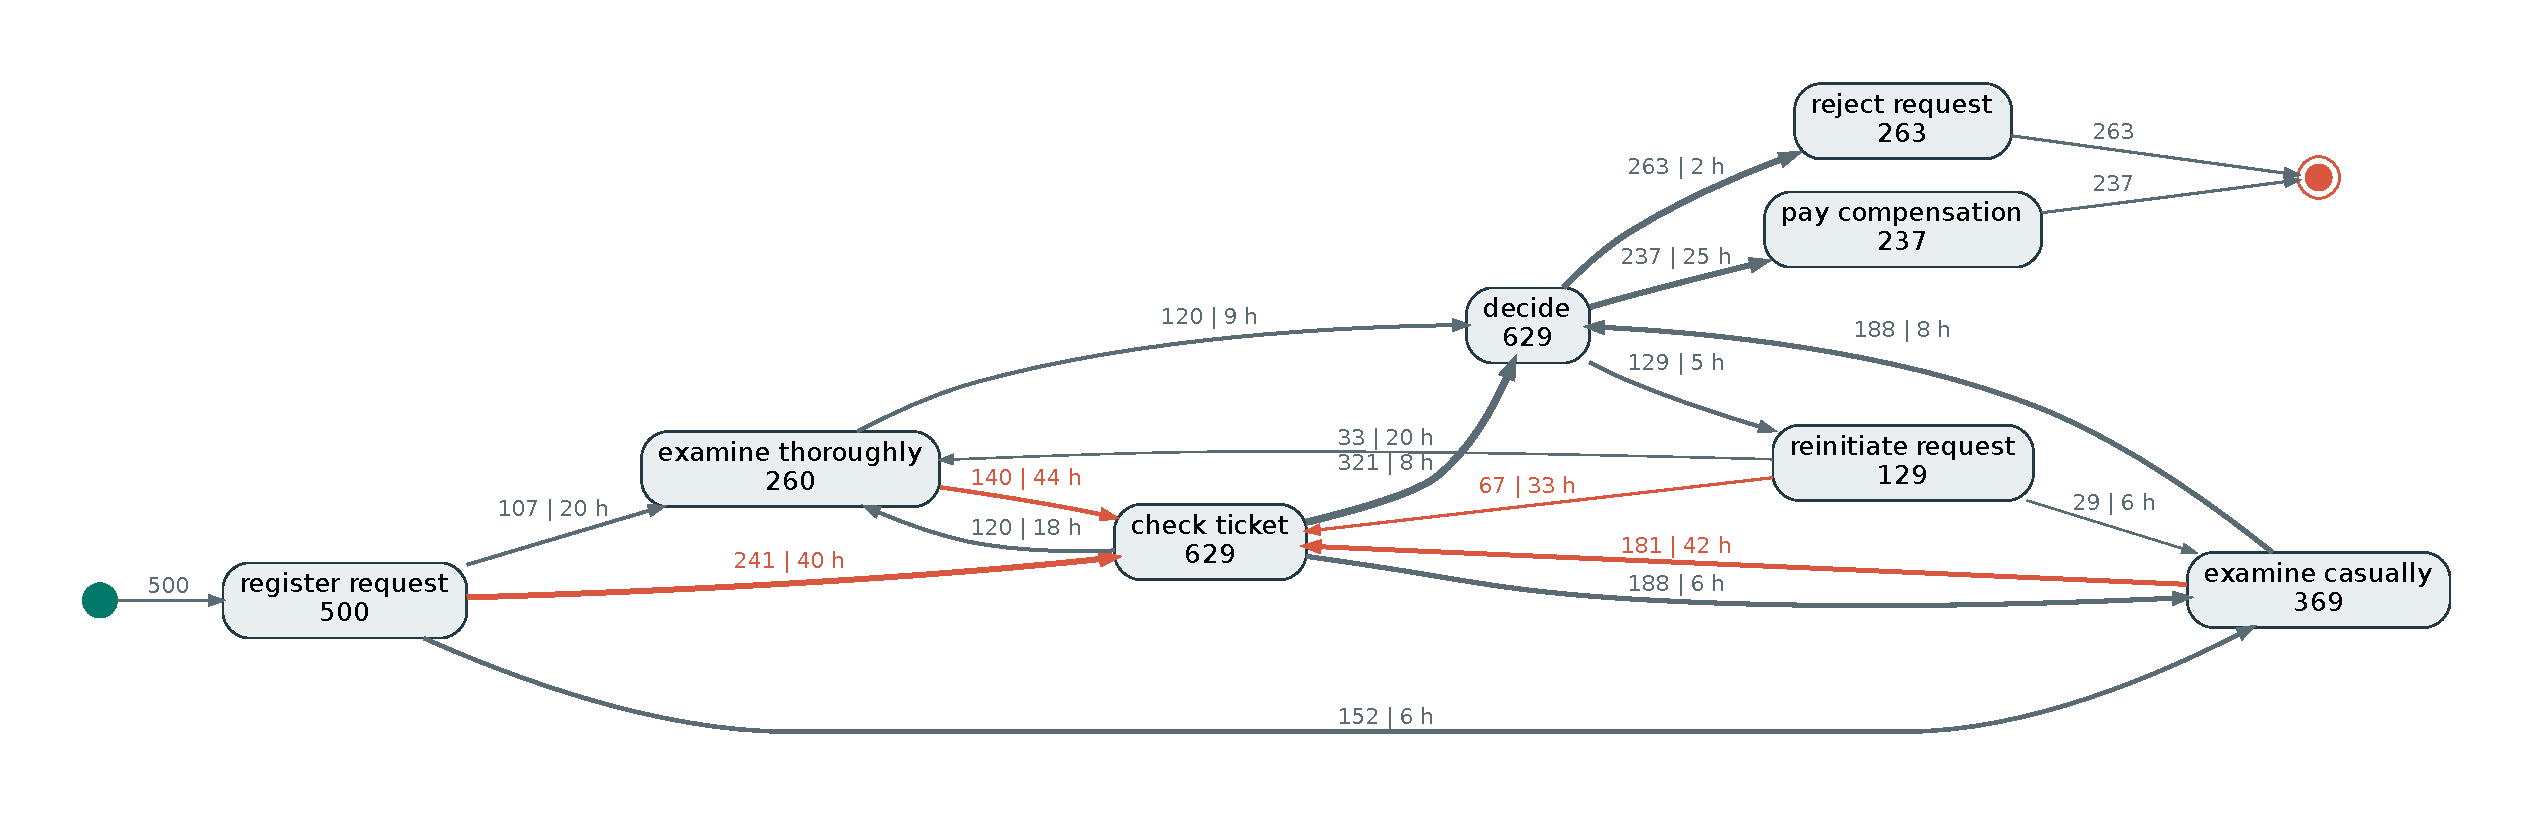
\includegraphics[width=\textwidth]{ch04/process_dfg}
\caption{Directly-follows graph of the compensation process. Nodes show the number of executions of each
activity; edges show the number of times the target directly follows the source and the mean time
between the two events. Edges slower than 30 hours are highlighted.}
\label{fig:dfg}
\end{figure}

\begin{figure}[htbp]
\centering
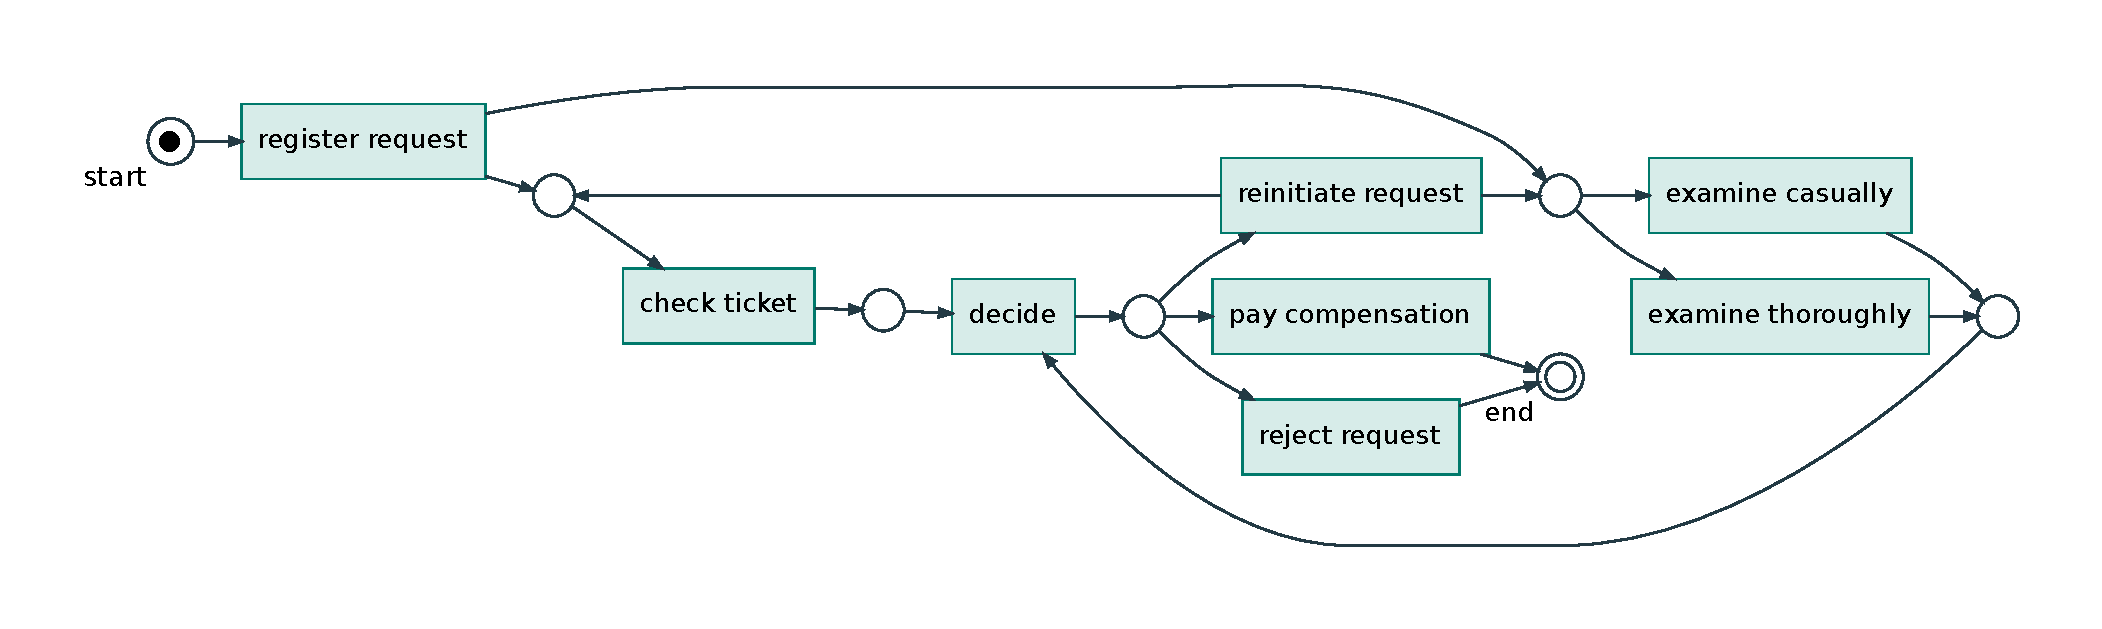
\includegraphics[width=0.92\textwidth]{ch04/process_petri}
\caption{Petri net discovered by the alpha algorithm. Boxes are transitions (activities), circles are
places; the token in the start place is the initial state.}
\label{fig:petri}
\end{figure}

The alpha algorithm is a clear introduction to process discovery, but it has well-known limitations:
it assumes that the log is complete and noise-free, and it cannot handle short loops or some
constructs. Practical algorithms, such as the heuristics miner \citep{weijters2006process}, which filters
infrequent behaviour, or the inductive miner \citep{leemans2013discovering}, which guarantees sound
models, are available in open-source tools such as ProM and PM4Py \citep{berti2019process}, and in
commercial products.

\subsection{Conformance checking}

Conformance checking\index{conformance checking} measures how well a model and a log agree. \emph{Token-based replay\index{token replay|textbf}}
\citep{rozinat2008conformance} plays each trace on the Petri net\index{Petri net}, firing the transition of each event: a
transition consumes a token from each of its input places and produces one in each of its output places.
If an input place is empty, the event did not respect the model, and a \emph{missing} token is created to
continue; tokens left in the net at the end are \emph{remaining}. With $p$, $c$, $m$ and $r$ the produced,
consumed, missing and remaining tokens over the whole log, the \emph{fitness\index{fitness|textbf}} is
\begin{equation}\label{eq:fitness}
  \mathrm{fitness}=\frac12\Bigl(1-\frac{m}{c}\Bigr)+\frac12\Bigl(1-\frac{r}{p}\Bigr),
\end{equation}
which is 1 when every trace can be replayed perfectly.

\begin{pylisting}[label={lst:conformance}]{Conformance checking by token-based replay}
from event_log import ACTIVITIES, simulate_log
from pm import alpha_miner, fitness, token_replay

code = {name: letter for letter, name in ACTIVITIES.items()}

def traces_of(log):
    log = log.sort_values(["case", "timestamp"])
    to_str = lambda s: "".join(code[a] for a in s)
    return list(log.groupby("case")["activity"].agg(to_str))

# the model is discovered from a clean log and checked against new cases
model = alpha_miner(traces_of(simulate_log(500, seed=0)))
for noise in (0.0, 0.1, 0.3):
    traces = traces_of(simulate_log(500, seed=1, noise=noise))  # new cases to check
    bad = [t for t in traces if token_replay(t, model)[2] > 0]  # missing tokens
    print(f"deviation rate {noise:.0%}: fitness {fitness(traces, model):.3f}, "
          f"{len(bad)} of {len(traces)} cases do not fit")
for t in bad[:2]:
    p, c, m, r = token_replay(t, model)
    print(f"case {t}: produced {p}, consumed {c}, missing {m}, remaining {r}")
\end{pylisting}
\begin{pyoutput}
deviation rate 0%: fitness 1.000, 0 of 500 cases do not fit
deviation rate 10%: fitness 0.987, 53 of 500 cases do not fit
deviation rate 30%: fitness 0.961, 155 of 500 cases do not fit
case abeg: produced 6, consumed 6, missing 1, remaining 1
case abedg: produced 7, consumed 7, missing 1, remaining 1
\end{pyoutput}

\Cref{lst:conformance} checks new cases against the net discovered from the clean log. Without deviations
the fitness is 1.000; when 10\% of the cases deviate (the ticket is not checked, or the decision is taken
before the examination or the check is finished) it falls to 0.987, and 53 of the 500 cases do not fit;
with 30\% of deviations, to 0.961, with 155 cases that do not fit. For the case $abeg$, which skips the
ticket check, the decision finds one of its input places empty (one missing token) and the token produced
for the check is never consumed (one remaining token): its own fitness is
$\frac12(1-\frac16)+\frac12(1-\frac16)=0.83$. Conformance checking tells the organisation how
often the rules are broken, which cases break them and where.

\subsection{Performance analysis}

Enriching the model with timestamps reveals where time is spent. In our log, the edges leading to the
ticket check take 40 to 44 hours on average, against roughly a day or less for the others (\cref{fig:dfg}). These are times between
consecutive recorded events: with completion events only, they mix service, waiting and the overlap of
concurrent activities (and our simple generator accumulates its timestamps sequentially, even where the
net allows concurrency), so they show where to look. They do not measure service durations. In this
simulation the ticket check is slow by construction, so speeding it up, or starting it earlier, would
shorten the whole process. Process mining\index{process mining} tools also
show the frequency of each variant, the workload of each resource, and the evolution of performance over
time, which links process mining with the monitoring\index{monitoring} of Unit~6.

% =====================================================================
\section{Robotic process automation}\label{sec:rpa}

\emph{Robotic process automation\index{robotic process automation (RPA)|textbf}} (RPA) tries to free people from the simple and repetitive tasks of
their daily work \citep{vanderaalst2018robotic,syed2020robotic}. It develops software agents, called
\emph{robots}, that mimic people performing business tasks on their computers: filling in forms,
processing the invoices received by e-mail, correcting mistakes in databases, copying data from one
application to another. RPA is widely adopted by companies and supported by vendors such as UiPath, Blue
Prism, Automation Anywhere and IBM. Its robots work through the same user interfaces as people, so they
can automate legacy systems that offer no programming interface, but they are brittle when the
interface changes.

\subsection{From RPA to intelligent process automation}

Most RPA\index{robotic process automation (RPA)} systems rely on explicitly encoded rules and configurations. Artificial intelligence
can extend these systems: \emph{intelligent process automation\index{intelligent process automation|textbf}} (IPA) aims to generalise RPA by
providing the tools to create complex workflows with minimal user intervention. The IEEE describes it as
a preconfigured software instance that combines business rules, experience-based context determination
logic and decision criteria to initiate and execute multiple interrelated human and automated processes
in a dynamic context \citep{ieee2017ipa}. A key step is the formalisation of workflows (the interaction
between the actions of the user, software and data artefacts) in a formal language that can be used to
simulate and execute them; the actions and events can be captured with tools that automate the graphical user interface (GUI), such as
Sikuli, which locates interface elements from screenshots \citep{yeh2009sikuli}. Discovering which
routines are worth automating from logs of user interactions is the goal of \emph{robotic process
mining\index{process mining|textbf}} \citep{leno2021robotic}, which brings together the two halves of this section.

\citet{ferreira2020evaluation} define IPA as a combination of four tasks between three representations of
a process (\cref{fig:ipa}): \begin{itemize}
\item \emph{Demo2text} describes in natural language a demonstration of a user
executing an activity; \item \emph{Demo2process} turns a demonstration into a program that can re-execute it;
\item \emph{Text2process} generates the process from a description of the activity, which is program synthesis
and inductive programming\index{inductive programming} (\cref{sec:indprog}); \item \emph{Process2text} describes in natural language a
process that is already implemented.
\end{itemize}

\begin{figure}[htbp]
\centering
\begin{tikzpicture}[font=\small\sffamily,
  rep/.style={draw=edmnavy,fill=edmnavy!6,rounded corners=3pt,minimum width=30mm,minimum height=10mm,align=center},
  arr/.style={-{Stealth[length=2.2mm]},edmteal,thick}]
  \node[rep] (demo) at (0,0) {demonstration\\(user actions)};
  \node[rep] (text) at (-3.4,-2.6) {natural language\\description};
  \node[rep] (proc) at (3.4,-2.6) {process\\(program)};
  \draw[arr] (demo) -- node[above left,text=edmnavy] {Demo2text} (text);
  \draw[arr] (demo) -- node[above right,text=edmnavy] {Demo2process} (proc);
  \draw[arr] ([yshift=2mm]text.east) -- node[above,text=edmnavy] {Text2process} ([yshift=2mm]proc.west);
  \draw[arr] ([yshift=-2mm]proc.west) -- node[below,text=edmnavy] {Process2text} ([yshift=-2mm]text.east);
\end{tikzpicture}
\caption{The four tasks of intelligent process automation \citep{ferreira2020evaluation}.}
\label{fig:ipa}
\end{figure}

\subsection{Two software robots}

In a visual RPA\index{robotic process automation (RPA)} tool such as UiPath, a robot is built by recording or assembling activities. A robot that
collects the prices of a product category from an online shop, for instance, is defined in five steps:
create a new process; open the web page of the category in the browser; select, with the data extraction wizard, one example of each field (the brand, the name and the price of a product); indicate the link to the next page,
so that the robot goes through all the pages; and add an activity that writes the extracted table to a CSV
file. From the examples of the third step, the tool infers the rest of the table, which is programming by example\index{programming by example} again. Then run it.

The same logic can be written in a few lines of code. \Cref{lst:rpa} is a robot that reads invoices
received by e-mail, extracts the supplier, the invoice number, the date and the amount, canonicalises
dates written in three formats and amounts written with European and English separators, and books the
invoices that pass the business rules. The cases it cannot handle, an invoice without a number and one
above the approval limit, are delegated to a person: as with the delegating\index{delegation} classifiers of
\cref{sec:cautious}, an automated system should recognise the cases it cannot handle. Each message is handled on its own, so an error in one does not stop the others; missing
fields, impossible dates (31 February) and unsupported amounts or currencies are delegated too, and the
output is written as proper CSV (the supplier ``Acme, SL'' contains a comma). The robot only prepares
records for booking: registering them in the accounting system is a separate step. Amounts are parsed only when they
match a declared format (European or English with two decimal places, or a plain integer): ambiguous amounts such as
12.480 or 12,3 are sent for human review, and the approval limit is applied to the canonical amount, never to a guessed
interpretation. The checks at the end of the listing are acceptance and rejection tests of this contract.

\begin{pylisting}[label={lst:rpa}]{A software robot that books invoices received by e-mail}
import csv
import re
import sys
from datetime import datetime
from decimal import Decimal, InvalidOperation

EMAILS = [  # the inbox the robot reads every morning
    "From: Ferreteria Sol\nSubject: Invoice INV-2041\nDate: 12/03/2026\n"
    "Total: 1.234,50 EUR",
    "From: Papeleria Mar\nSubject: Factura F-778\nFecha: 2026-03-15\nImporte: 89,90 EUR",
    "From: Tech Supplies Ltd\nSubject: Invoice no. 5531\nDate: 15 March 2026\n"
    "Amount due: EUR 12,480.00",
    "From: Limpiezas Turia\nSubject: Monthly service\nDate: 18/03/2026\n"
    "Total: 640,00 EUR",
    "From: Imprenta Rapida\nSubject: Factura F-2026-31\nFecha: 20/03/2026\n"
    "Total: 312,75 EUR",
    "From: Acme, SL\nSubject: Invoice INV-77\nDate: 31/02/2026\nTotal: 45,00 EUR"]
LIMIT = Decimal(10_000)                            # larger amounts need a manager

def parse_date(text):                              # None if impossible or unknown
    for fmt in ("%d/%m/%Y", "%Y-%m-%d", "%d %B %Y"):   # month names: English locale
        try:
            return datetime.strptime(text.strip(), fmt).date().isoformat()
        except ValueError:
            pass

FORMATS = {                                        # the only accepted amount formats
    "european": r"-?\d{1,3}(?:\.\d{3})+,\d{2}|-?\d+,\d{2}",     # 1.234,50  89,90
    "english": r"-?\d{1,3}(?:,\d{3})+\.\d{2}|-?\d+\.\d{2}",    # 12,480.00  89.90
    "integer": r"-?\d+"}                                       # 5

def parse_amount(line):
    """(amount, currency) if the whole field matches a declared format, else (None, None):
    ambiguous amounts such as 12.480 or 12,3 are never guessed."""
    cur = r"(EUR|USD|GBP)"
    m = re.fullmatch(rf"[^:]*:\s*(?:{cur}\s+)?(-?[\d.,]+)(?:\s+{cur})?\s*", line)
    if m is None or bool(m.group(1)) == bool(m.group(3)):     # exactly one currency
        return None, None
    number, currency = m.group(2), m.group(1) or m.group(3)
    if re.fullmatch(FORMATS["european"], number):
        number = number.replace(".", "").replace(",", ".")
    elif re.fullmatch(FORMATS["english"], number):
        number = number.replace(",", "")
    elif not re.fullmatch(FORMATS["integer"], number):
        return None, None
    return Decimal(number), currency

out = csv.writer(sys.stdout, lineterminator="\n")  # quotes fields when needed
out.writerow(["invoice", "date", "supplier", "amount", "status"])
for email in EMAILS:                               # every message is handled on its own
    supplier = re.search(r"From: (.+)", email)
    number = re.search(r"(?:Invoice|Factura)(?: no\.)? ([A-Z]+-[\d-]+|\d+)", email)
    date = re.search(r"(?:Date|Fecha): (.+)", email)
    date = parse_date(date.group(1)) if date else None
    amount, currency = parse_amount(email.splitlines()[-1])
    if number is None or supplier is None:
        status = "to human: no invoice number"
    elif date is None:
        status = "to human: missing or invalid date"
    elif amount is None or currency != "EUR" or amount <= 0:
        status = "to human: amount or currency not supported"
    elif amount > LIMIT:
        status = "to human: needs approval"
    else:
        status = "ready for booking"
    out.writerow([number.group(1) if number else "?", date or "?",
                  supplier.group(1) if supplier else "?",
                  f"{amount:.2f}" if amount is not None else "?", status])

print("\nformat checks (acceptance and rejection tests):")
for field in ["Total: 12.480 EUR", "Total: 12,3 EUR", "Total: 5 EUR",
              "Total: 1.234,50 EUR", "Total: 1,234.50 EUR", "Total: -1.234,50 EUR"]:
    amount, currency = parse_amount(field)
    print(f"  {field:22s} -> {'to human' if amount is None else f'{amount} {currency}'}")
\end{pylisting}
\begin{pyoutput}
invoice,date,supplier,amount,status
INV-2041,2026-03-12,Ferreteria Sol,1234.50,ready for booking
F-778,2026-03-15,Papeleria Mar,89.90,ready for booking
5531,2026-03-15,Tech Supplies Ltd,12480.00,to human: needs approval
?,2026-03-18,Limpiezas Turia,640.00,to human: no invoice number
F-2026-31,2026-03-20,Imprenta Rapida,312.75,ready for booking
INV-77,?,"Acme, SL",45.00,to human: missing or invalid date

format checks (acceptance and rejection tests):
  Total: 12.480 EUR      -> to human
  Total: 12,3 EUR        -> to human
  Total: 5 EUR           -> 5 EUR
  Total: 1.234,50 EUR    -> 1234.50 EUR
  Total: 1,234.50 EUR    -> 1234.50 EUR
  Total: -1.234,50 EUR   -> -1234.50 EUR
\end{pyoutput}

% =====================================================================
\section{Summary}\label{sec:summary4}

\begin{itemize}
  \item The steps of a data science project are automatable in very different degrees: modelling
        almost completely, data preparation and exploration partially, problem analysis and
        communication hardly at all.
  \item Data wrangling\index{data wrangling}, exploratory analysis and feature engineering\index{feature engineering} have many tools; deep feature
        synthesis\index{deep feature synthesis} generates features from relational data automatically.
  \item AutoML\index{AutoML} solves the combined algorithm selection\index{algorithm selection} and hyperparameter optimisation\index{hyperparameter optimisation} problem with
        random search\index{random search}, Bayesian optimisation\index{Bayesian optimisation}, multi-fidelity or evolutionary methods. The score of the
        selected configuration is optimistic, so the whole search must be evaluated on unseen data.
  \item Metalearning\index{metalearning} learns from previous experiments, for instance to select algorithms from
        meta-features; its value is bounded by how complementary the candidate algorithms are.
  \item Inductive programming\index{inductive programming} synthesises programs from examples and background knowledge\index{background knowledge}, in logic or
        functional languages; inductive bias\index{inductive bias} and domain-specific languages\index{domain-specific language} make the search tractable,
        and language models now act as few-shot inductive programmers.
  \item Large language models\index{large language model (LLM)} assist at every stage of a project and, as agents, carry out whole analyses;
        because their code can be plausible and wrong (hallucinated columns, leakage\index{data leakage}, silently dropped rows),
        it must be verified automatically: isolated execution, invariants and held-out evaluation.
  \item Genetic programming\index{genetic programming} evolves programs, represented as trees, by selection, crossover\index{genetic programming!crossover} and
        mutation\index{genetic programming!mutation}.
  \item Process mining\index{process mining} discovers, checks and enhances process models from event logs\index{event log}; robotic and
        intelligent process automation\index{intelligent process automation} build software robots that perform repetitive tasks.
\end{itemize}

\section*{Bibliographic notes}
\phantomsection\addcontentsline{toc}{section}{Bibliographic notes}

\citet{martinezplumed2021crisp} review data science processes from CRISP-DM\index{CRISP-DM} to data science trajectories.
\citet{hutter2019automated} is a standard reference on AutoML\index{AutoML}, and \citet{zoller2021benchmark} survey and
benchmark AutoML frameworks; \citet{brazdil2022metalearning} cover metalearning\index{metalearning} in depth.
\citet{gulwani2015inductive} present inductive programming\index{inductive programming} and its applications to end users, and
\citet{jaimovitch2023can} study language models for data wrangling\index{data wrangling}. \citet{debie2022automating} discuss what automating
data science\index{automated data science} means, and \citet{tornede2024automl} the opportunities and risks of large language models\index{large language model (LLM)} for AutoML. \citet{poli2008field} is a free field
guide to genetic programming\index{genetic programming}. \citet{vanderaalst2016process} is a reference book on process mining\index{process mining}, and
\citet{syed2020robotic} review the themes and challenges of RPA\index{robotic process automation (RPA)}.

\section*{Exercises}
\phantomsection\addcontentsline{toc}{section}{Exercises}

\begin{enumerate}[label=\textbf{4.\arabic*},ref=4.\arabic*,leftmargin=*,itemsep=6pt]
  \item\label{exr4:grid} A budget of nine evaluations is spent on two hyperparameters, only one of which
        matters. How many distinct values of the important hyperparameter does a $3\times3$ grid try? And
        random search\index{random search}?
  \item\label{exr4:ei} The best accuracy found so far is $f^\star=0.86$. A Gaussian process predicts
        $\mu=0.85$, $\sigma=0.02$ for configuration $z_1$ and $\mu=0.80$, $\sigma=0.06$ for $z_2$. Compute
        the expected improvement of both (\cref{eq:ei}). Which one is evaluated next, and why?
  \item\label{exr4:sh} Successive halving starts with 81 configurations, a budget $r$ each and $\eta=3$.
        How many configurations and what budget per configuration are there in each round? Compare the
        total budget with evaluating the 81 configurations with the final budget.
  \item\label{exr4:optimism} In \cref{lst:cash}, with 200 configurations the winner has a cross-validation
        accuracy of 0.950 and a test accuracy of 0.925. Explain the difference and design a protocol that
        gives an honest estimate of the performance of the AutoML\index{AutoML} process.
  \item\label{exr4:meta} Compute the following meta-features of a data set with 1000 examples, 20 features
        and classes of 900 and 100 examples: $\log_{10}n$, $\log_{10}d$, $n/d$, the minority fraction and
        the class entropy (in bits).
  \item\label{exr4:ilp} With the background predicates \texttt{parent/2}, \texttt{male/1} and
        \texttt{female/1}, write a clause for \texttt{grandmother(X,Y)}. How many literals does its body
        need, and why must it use a variable that does not appear in the head?
  \item\label{exr4:bias} How many sequences of $d=4$ functions can be formed with $b=5$ and with $b=20$
        background functions? How many ordered binary expressions with four operator nodes are there with
        those numbers of binary operators and three terminals (use $C_4=14$)? What does this tell you about
        the value of domain-specific languages\index{domain-specific language}?
  \item\label{exr4:pbe} With the DSL of \cref{lst:pbe}, write a program for the example
        \texttt{Ferri, Cesar} $\mapsto$ \texttt{C. Ferri}. Find the four shortest programs consistent with this single
        example and their outputs for \texttt{Garcia Lopez, Juan Jose}.
  \item\label{exr4:cross} In \cref{fig:gptrees}, which child results from replacing the leaf 3 of the second
        parent by the subtree $x\times x$ of the first?
  \item\label{exr4:alpha} Apply the alpha algorithm\index{alpha algorithm} to the log $L=\{abcd, acbd, aed\}$: compute the
        relations $\rightarrow$, $\parallel$ and $\#$ and the places of the Petri net\index{Petri net}.
  \item\label{exr4:replay} Replay the trace $abd$ on the net of Exercise~\ref{exr4:alpha} and compute its
        fitness\index{fitness}.
  \item\label{exr4:rpa} Classify each scenario as RPA\index{robotic process automation (RPA)} or IPA\index{intelligent process automation}: (a) a robot copies the fields of a web form
        into the accounting system following fixed rules; (b) a system watches an employee process a few
        claims and learns a program that processes new ones; (c) a system writes, from the code of a robot,
        a description of what it does for the auditors.
  \item\label{exr4:prompt} Write a few-shot prompt\index{prompt} that asks a language model to turn dates such as
        \texttt{23/12/2021} into \texttt{Dec 23, 2021}. How would you check the outputs before applying the
        transformation to a column of a million dates?
  \item\label{exr4:llmstage} Choose two stages of \cref{tab:llmstages}. For each, describe a task you would
        delegate to a language model assistant and an automatic check you would apply to its output.
  \item\label{exr4:verify} Which check of \cref{lst:assistant} catches each proposal? (a)
        \texttt{df["x"] = df["balance"] / df["limit"]} on a table without those columns; (b) the default rate of
        each customer's branch, computed on the whole table; (c) code that removes the customers with a missing
        income before computing a feature; (d) a feature that raises the cross-validated AUC by 0.001.
  \item\label{exr4:memorise} Without being given any training data, a language model predicts the survival of the
        Titanic passengers surprisingly well. Give two explanations, and say how you would evaluate its abilities
        fairly.
\end{enumerate}

\section*{Solutions to selected exercises}
\phantomsection\addcontentsline{toc}{section}{Solutions to selected exercises}

\begin{description}[font=\bfseries,leftmargin=0pt,itemsep=5pt]
  \item[\ref{exr4:grid}] The grid tries 3 values of each hyperparameter; random search\index{random search} tries 9 different
        values of each (with probability 1 for continuous ranges), so it explores the important one three
        times more finely.
  \item[\ref{exr4:ei}] For $z_1$, $u=-0.5$ and $\mathrm{EI}=0.02\,[-0.5\cdot0.3085+0.3521]=0.0040$. For $z_2$,
        $u=-1$ and $\mathrm{EI}=0.06\,[-1\cdot0.1587+0.2420]=0.0050$. The second point is evaluated: its mean is
        lower, but its uncertainty gives it a better chance of a large improvement (exploration).
  \item[\ref{exr4:sh}] Rounds of $81,27,9,3,1$ configurations with budgets $r,3r,9r,27r,81r$: each round costs
        $81r$, in total $405r$, against $81\cdot81r=6561r$, sixteen times more.
  \item[\ref{exr4:optimism}] The winner is the configuration with the highest cross-validation score among
        200, partly by luck, so its score is biased upwards. Evaluate the whole search with nested
        cross-validation\index{cross-validation!nested}, or run it on a training set and report the score of the final model on a
        separate test set that the search never uses.
  \item[\ref{exr4:meta}] $\log_{10}n=3$, $\log_{10}d=1.30$, $n/d=50$, minority fraction 0.1, and entropy
        $-0.9\log_20.9-0.1\log_20.1=0.469$ bits.
  \item[\ref{exr4:ilp}] \texttt{grandmother(X,Y) :- parent(X,Z), parent(Z,Y), female(X).} Three literals; the
        variable \texttt{Z}, the intermediate parent, connects $X$ and $Y$ and is not in the head.
  \item[\ref{exr4:bias}] Sequences: $5^4=625$ and $20^4=160{,}000$. Expressions: $C_4\,b^4\,3^5$, that is
        $14\cdot625\cdot243=2{,}126{,}250$ and $14\cdot160{,}000\cdot243=544{,}320{,}000$. The count depends on the
        grammar, but in every case a small, specialised set of functions keeps the space small enough to
        search, which is what DSLs\index{domain-specific language} provide.
  \item[\ref{exr4:pbe}] The program \texttt{initial(word,1)} + \texttt{". "} + \texttt{token(word,0)}. Eight programs are consistent with the example. The four shortest combine
        \texttt{initial(word,1)} or \texttt{initial(word,-1)} with \texttt{token(word,0)} or
        \texttt{token(word,-2)}; for the new input they give \texttt{L. Garcia}, \texttt{L. Juan},
        \texttt{J. Garcia} and \texttt{J. Juan}. The other four are longer variants that split the separator \texttt{". "} into two
        constants and behave in the same way. The intended answer (\texttt{J. Garcia}) needs more examples,
        or a richer DSL.
  \item[\ref{exr4:cross}] $xy-x^2$.
  \item[\ref{exr4:alpha}] $a\rightarrow b$, $a\rightarrow c$, $a\rightarrow e$, $b\rightarrow d$, $c\rightarrow d$,
        $e\rightarrow d$, $b\parallel c$, and $a\#d$, $b\#e$, $c\#e$ (pairs that never directly follow each
        other: $a$ and $d$ appear in every trace, so $\#$ does not mean exclusive choice). Places: $(\{a\},\{b,e\})$, $(\{a\},\{c,e\})$,
        $(\{b,e\},\{d\})$, $(\{c,e\},\{d\})$, plus the source place before $a$ and the sink place after $d$.
  \item[\ref{exr4:replay}] $a$ consumes the start token and produces two; $b$ consumes one and produces one;
        $d$ needs tokens in $(\{b,e\},\{d\})$, present, and $(\{c,e\},\{d\})$, missing; finally the end token is
        consumed. $p=5$, $c=5$, $m=1$, $r=1$ (the token for $c$), so the fitness\index{fitness} is
        $\frac12(1-\frac15)+\frac12(1-\frac15)=0.8$.
  \item[\ref{exr4:rpa}] (a) RPA\index{robotic process automation (RPA)}. (b) IPA\index{intelligent process automation} (Demo2process). (c) IPA (Process2text).
  \item[\ref{exr4:prompt}] For instance: \texttt{input: 23/12/2021, output: Dec 23, 2021; input: 05/01/2022,
        output: Jan 5, 2022; input: 31/07/2023, output:}. Check the outputs on held-out examples with known
        answers, validate their format with a regular expression, and compare the parsed dates with the
        inputs (same day, month and year) before trusting the transformation.
  \item[\ref{exr4:llmstage}] For example, data preparation: ask for the code that standardises the dates of a
        column, and check that the number of rows is unchanged and that the result matches a few dates converted by
        hand. Modelling: ask for a pipeline, and check that the preprocessing is fitted inside the cross-validation
        and that the model beats a simple baseline on held-out data.
  \item[\ref{exr4:verify}] (a) Running the code: the columns do not exist (a hallucination). (b) Running it without the
        target: the default rate uses the target (leakage\index{data leakage}). (c) The invariant on the rows. (d) The minimum gain: an
        improvement of 0.001 is within the noise of cross-validation.
  \item[\ref{exr4:memorise}] The data set is very likely in its training data, so it may have memorised it
        (contamination\index{contamination of benchmarks}); and texts about the Titanic describe its patterns (women and children first, the classes of the
        cabins). A fair evaluation uses data the model cannot have seen, such as recent or private data, or a perturbed
        version of the data set, and compares the model with a classifier trained on the same information.
\end{description}


% =====================================================================
%  Unit 5 -- Deployment of models
%  (this file is assembled from src/ch05/*.tex by build_chapter.py)
% =====================================================================
\chapter{Deployment of Models}\label{ch:deployment}

On the morning of 1 August 2012, Knight Capital, one of the largest traders of American equities, started using new
software on the servers that sent its orders to the stock market. A technician had not copied the new code to one of
the eight servers, where an obsolete function, reactivated by a flag that the new code reused, began to send orders
that nobody had intended. In 45 minutes the firm lost more than 460 million dollars; it had to be rescued by investors
and was taken over the following year \citep{sec2013knight}. Knight's software was not a machine learning model, but
its failure is the nightmare of every deployment: a manual step, no automated check that every server ran the same
version, and no quick way of stopping. Deploying models adds risks of its own to these.

A prediction model creates value only when its users can reach its outputs reliably. Deployment is the step that puts a model in front
of its users, and it is where many data science projects fail: surveys of practitioners describe
models that worked in the laboratory and never reached production, or reached it and broke
\citep{paleyes2022challenges}. This unit covers the two halves of the problem. The first is
choosing \emph{how} a model will serve its predictions: on a server that answers requests one by
one or in batches, on the user's own device, and, for training, federated learning, which learns
from data that stay on the devices and can produce a shared model or personalised ones. The second is building the \emph{infrastructure} that makes deployment
reliable and repeatable: version control for code and data, experiment tracking, automated tests,
packaging, and pipelines that retrain and redeploy models automatically, a set of practices known
as ModelOps or MLOps \citep{kreuzberger2023mlops}. We follow the approach of
\citet{ameisen2020building} for the first half and of \citet{dubovikov2019managing} for the
second.

\begin{objectives}
After studying this unit you should be able to:
\begin{itemize}
  \item choose a deployment option (server-side streaming or batch, client-side on device or in
        the browser, federated learning) from the latency, hardware, network, privacy, cost and
        complexity requirements of an application;
  \item build a prediction API, and measure its latency and throughput;
  \item make a model small enough for a device, and explain how federated learning trains
        personalised models without collecting the data;
  \item exchange models between platforms with standard formats such as PMML and ONNX, and
        build and test a small web application for a model;
  \item explain ModelOps and its relation to DevOps, and set up version control for code and data,
        reproducible environments and experiment tracking;
  \item write automated tests for data science code, package it, and design a continuous training
        pipeline with data tests and quality gates;
  \item assemble a technology stack for a data science team.
  \item deploy applications built on large language models: choose where the model runs, treat prompts
        as code, build and evaluate retrieval-augmented generation, and add guardrails;
\end{itemize}
\end{objectives}

% =====================================================================
\section{Choosing a deployment option}\label{sec:deployoptions}

Different deployment approaches suit different requirements. Before choosing one we must consider
the \emph{latency} the application can tolerate, the \emph{hardware} and \emph{network} available
at prediction time, the \emph{privacy} of the data, the \emph{cost} of running the system and the
\emph{complexity} we can afford to maintain. \Cref{tab:deploy} summarises how the options of this
section compare.

\begin{table}[htbp]
\centering\small
\caption{Deployment options and their trade-offs.}\label{tab:deploy}
\begin{tabularx}{\textwidth}{@{}>{\raggedright\arraybackslash}p{2.5cm}>{\raggedright\arraybackslash}X>{\raggedright\arraybackslash}X@{}}
\toprule
Option & When it fits & Main costs and risks\\
\midrule
Server, streaming (API) & the data needed are known only at request time and the prediction is
needed immediately & servers that scale with the number of users; a central point of failure\\
Server, batch & the features are available before the prediction is needed & predictions can be
stale; storage of precomputed results\\
Client, on device & low latency without network, offline use, sensitive data & small models,
possible loss of accuracy, one optimisation per type of device\\
Client, browser & interactive applications without installation & the model is downloaded by every
visitor\\
Federated learning (training) & the training data must stay on the devices; it learns a shared model, which
can then be personalised &
much greater complexity: training, aggregation and privacy on many devices\\
\bottomrule
\end{tabularx}
\end{table}

\subsection{Server-side deployment}

Server-side deployment sets up a web server that accepts requests from clients, runs them through an
inference pipeline, and returns the results. There are two common workloads: \emph{streaming}, in
which each request is answered as it arrives, and \emph{batch}, in which predictions are computed in
advance for many examples (\cref{fig:serverflows}).

\begin{figure}[htbp]
\centering
\begin{tikzpicture}[font=\scriptsize\sffamily,
  st/.style={draw=edmnavy,fill=edmnavy!6,rounded corners=2pt,minimum height=8mm,minimum width=15.5mm,align=center},
  ds/.style={cylinder,shape border rotate=90,draw=edmnavy,fill=edmbronze!25,aspect=0.25,minimum width=11mm,minimum height=8mm,align=center},
  arr/.style={-{Stealth[length=1.6mm]},edmnavy},
  lab/.style={font=\scriptsize\sffamily\bfseries,text=edmnavy,anchor=east,align=right}]
  \node[lab] at (-0.95,0) {streaming\\(per request)};
  \node[st] (r) at (0,0) {request};
  \node[st] (v) at (1.95,0) {validate};
  \node[st] (g) at (3.9,0) {gather\\more data};
  \node[st] (p) at (5.85,0) {pre-\\process};
  \node[st] (m) at (7.8,0) {run the\\model};
  \node[st] (o) at (9.75,0) {post-\\process};
  \node[st] (s) at (11.7,0) {send the\\result};
  \node[ds] (d1) at (3.9,-1.35) {store};
  \foreach \a/\b in {r/v,v/g,g/p,p/m,m/o,o/s} \draw[arr] (\a) -- (\b);
  \draw[arr,{Stealth[length=1.6mm]}-{Stealth[length=1.6mm]}] (g) -- (d1);
  \begin{scope}[yshift=-3.1cm]
  \node[lab] at (-0.95,0) {batch\\(scheduled)};
  \node[st] (bg) at (0.98,0) {gather all\\the data};
  \node[st] (bp) at (3.9,0) {pre-\\process all};
  \node[st] (bm) at (6.83,0) {run the\\model};
  \node[st] (bo) at (9.75,0) {post-\\process};
  \node[ds] (bs) at (11.7,0) {stored\\results};
  \foreach \a/\b in {bg/bp,bp/bm,bm/bo,bo/bs} \draw[arr] (\a) -- (\b);
  \end{scope}
  \begin{scope}[yshift=-4.75cm]
  \node[lab] at (-0.95,0) {batch\\(per request)};
  \node[st] (qr) at (0,0) {request};
  \node[st,minimum width=26mm] (ql) at (5.85,0) {look up the\\stored prediction};
  \node[st] (qs) at (9.75,0) {send the\\result};
  \draw[arr] (qr) -- (ql);
  \draw[arr] (ql) -- (qs);
  \draw[arr,dashed] (bs.south) -- ++(0,-0.25) -| (ql.north);
  \end{scope}
\end{tikzpicture}
\caption{Server-side inference. A streaming request goes through the whole pipeline; a batch job
computes the predictions in advance, and requests only look them up.}
\label{fig:serverflows}
\end{figure}

\paragraph{Streaming applications} The streaming approach treats the model as an \emph{endpoint}
to which users send requests; the users can be the end users of an application or an internal
service that relies on the predictions (for instance, a service that adjusts the number of servers
to the predicted traffic of a website). The code path of a request goes through six steps:
\emph{validate} the request (its values and the caller's permissions), \emph{gather} any additional
data the model needs, \emph{preprocess} the data, \emph{run} the model, \emph{postprocess} the results
(check that they are within bounds, make them understandable) and \emph{return} them. A streaming
approach is needed when the information the model requires is available only at prediction time and
the prediction is required immediately: a ride-hailing application that quotes the price of a trip
needs the user's location and the current availability of drivers, which exist only when the user
asks.

\Cref{lst:api} implements such an endpoint with Flask, the framework used by the ML Editor example of
\citet{ameisen2020building}. It follows the six steps, and its response codes tell the client what
went wrong: a valid request gets a probability, a decision and the version of the model (always
worth returning, for debugging and monitoring); a non-numeric value or a value out of range gets a
400 error, an unknown customer a 404, and a wrong key a 401. With Flask's test client, which skips
the network, a request takes less than a millisecond. In production the application runs behind a
WSGI server with several workers, and usually behind a load balancer.

\begin{pylisting}[label={lst:api}]{A prediction API with Flask, following the six steps of a request}
import time
import numpy as np
from flask import Flask, jsonify, request
from sklearn.datasets import make_classification
from sklearn.ensemble import GradientBoostingClassifier

# Offline: train the model and fill a feature store with data known before any request
X, y = make_classification(n_samples=3000, n_features=4, n_informative=4, n_redundant=0,
                           random_state=0)
model = GradientBoostingClassifier(random_state=0).fit(X, y)
store = {f"c{i:04d}": X[i, 2:] for i in range(len(X))}       # history of each customer
VERSION = "1.3.0"
app = Flask(__name__)

@app.post("/predict")
def predict():
    body = request.get_json(silent=True)
    if not isinstance(body, dict):                          # 1. validate: structure,
        return jsonify(error="a JSON object is required"), 400
    if body.get("api_key") != "secret":                     #    permissions
        return jsonify(error="not authorised"), 401
    if not isinstance(body.get("customer"), str):
        return jsonify(error="customer must be a string"), 400
    try:                                                    #    and values
        if any(isinstance(body.get(k), bool) for k in ("f1", "f2")):
            raise TypeError
        x = np.array([float(body["f1"]), float(body["f2"])])
    except (KeyError, TypeError, ValueError, OverflowError):
        return jsonify(error="f1 and f2 must be numbers"), 400
    if not np.isfinite(x).all() or np.any(np.abs(x) > 10):
        return jsonify(error="f1 and f2 must be finite and in [-10, 10]"), 400
    history = store.get(body["customer"])                         # 2. gather more data
    if history is None:
        return jsonify(error="unknown customer"), 404
    features = np.r_[x, history].reshape(1, -1)                   # 3. preprocess
    p = float(model.predict_proba(features)[0, 1])                # 4. run the model
    return jsonify(probability=p, version=VERSION,                # 5. postprocess
                   decision="accept" if p >= 0.5 else "reject")   # 6. return

client = app.test_client()                 # in production: an HTTP server and clients
good = {"api_key": "secret", "customer": "c0007", "f1": 0.5, "f2": -1.2}
requests = [good, {**good, "f1": "high"}, {**good, "f1": "NaN"}, [1, 2],
            {**good, "customer": "c9999"}, {**good, "f2": 45},
            {**good, "api_key": "guess"}]
for body in requests:
    r = client.post("/predict", json=body)
    print(r.status_code, r.get_json())
start = time.perf_counter()
for _ in range(200):
    client.post("/predict", json=good)
print(f"mean latency: {(time.perf_counter() - start) / 200 * 1000:.1f} ms per request")
\end{pylisting}
\begin{pyoutput}
200 {'decision': 'reject', 'probability': 0.2614178950022486, 'version': '1.3.0'}
400 {'error': 'f1 and f2 must be numbers'}
400 {'error': 'f1 and f2 must be finite and in [-10, 10]'}
400 {'error': 'a JSON object is required'}
404 {'error': 'unknown customer'}
400 {'error': 'f1 and f2 must be finite and in [-10, 10]'}
401 {'error': 'not authorised'}
mean latency: 0.5 ms per request
\end{pyoutput}

The validation step rejects malformed requests (a list instead of an object, a text or an infinite value
where a number is expected) with an error 400 before the model is called, and the probability is
returned without rounding, so that a client can reproduce the decision from it.

The endpoint approach is quick to implement, but the infrastructure has to grow with the number of
users: if the traffic exceeds the capacity of the servers, requests are delayed or fail. A useful tool
for sizing it is \emph{Little's law} \citep{little1961proof}: in a stable system, the mean number of
requests being served, $L$, equals the arrival rate $\lambda$ times the mean time each request spends
in the system, $W$,
\begin{equation}\label{eq:little}
  L=\lambda\,W .
\end{equation}
At 200 requests per second and 50 milliseconds per request, 10 requests are in progress on average,
so a server that can handle four at a time is not enough. Means are not the whole story: users
experience the \emph{tail} of the latency distribution, and in systems that call many services a few
slow responses dominate the user experience, which is why latency objectives are stated as high
percentiles such as p95 or p99 \citep{dean2013tail}.

\paragraph{Batch predictions} A batch job runs a model on many examples at a scheduled time and stores
the predictions, so that they can be looked up when they are needed. It is appropriate when the
features are available before the prediction is required. A model that helps salespeople decide which
prospects to contact can be trained on historical conversations and market trends, all known in
advance, and score every prospect overnight; an application that ranks the notifications a user
should read in the morning can process all unread messages in one batch before the user wakes up. A
batch approach needs as many inferences as a streaming one, but it is more resource efficient:
because the number of predictions is known at the start, resources are easy to allocate and
parallelise, and many examples can be processed per call. And at request time, looking up a stored
prediction is faster than computing it.

\begin{pylisting}[label={lst:latency}]{Latency of single requests and throughput of batches}
import time
import numpy as np
from sklearn.datasets import make_classification
from sklearn.ensemble import RandomForestClassifier

X, y = make_classification(n_samples=20000, n_features=20, random_state=0)
model = RandomForestClassifier(200, n_jobs=1, random_state=0).fit(X[:5000], y[:5000])
pool = X[5000:]

latency = []                                       # streaming: one request per call
for i in range(500):
    start = time.perf_counter()
    model.predict_proba(pool[i:i + 1])
    latency.append((time.perf_counter() - start) * 1000)
p50, p95, p99 = np.percentile(latency, [50, 95, 99])
print(f"single requests: p50 {p50:.1f} ms, p95 {p95:.1f} ms, p99 {p99:.1f} ms")

throughput = {}                                    # batch: many examples per call
for size in (1, 10, 100, 1000, 10000):
    reps = max(3, 300 // size)
    start = time.perf_counter()
    for _ in range(reps):
        model.predict_proba(pool[:size])
    throughput[size] = size * reps / (time.perf_counter() - start)
    print(f"batches of {size:5d}: {throughput[size]:9,.0f} predictions per second")
\end{pylisting}
\begin{pyoutput}
single requests: p50 9.9 ms, p95 10.5 ms, p99 11.2 ms
batches of     1:       101 predictions per second
batches of    10:       969 predictions per second
batches of   100:     7,305 predictions per second
batches of  1000:    31,478 predictions per second
batches of 10000:    57,923 predictions per second
\end{pyoutput}

\Cref{lst:latency} and \cref{fig:serving} quantify the difference for a random forest of 200 trees. A
single request takes about 10 milliseconds (p50 9.9, p95 10.5 and p99 11.2), so one process answers
about 100 requests per second. Called with batches of 10,000 examples, the same model produces about
58,000 predictions per second, almost 600 times more, because the fixed cost of each call (checking
the input, dispatching to the 200 trees) is shared by many examples.

\begin{figure}[htbp]
\centering
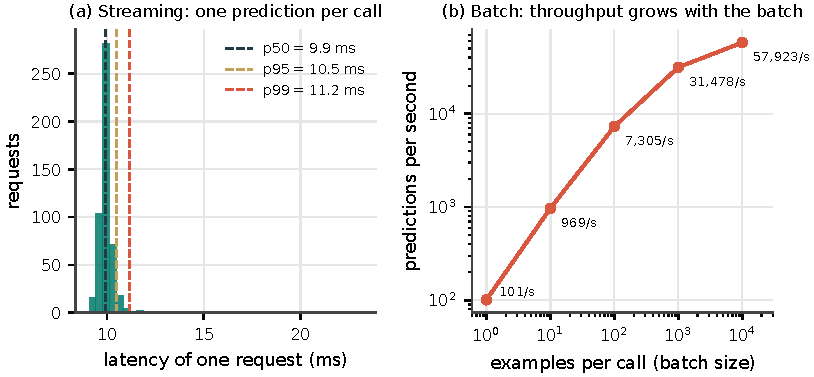
\includegraphics[width=\textwidth]{ch05/serving_latency}
\caption{(a) Latency of 500 single-example requests to a random forest, with its percentiles.
(b) Throughput as a function of the number of examples per call (both axes logarithmic).}
\label{fig:serving}
\end{figure}

A \emph{hybrid} approach precomputes as many cases as possible and, at inference time, either retrieves
the stored result or computes it on the spot if it is missing or outdated. It combines the speed of
batch with the freshness of streaming, at the price of a significantly more complex system. All
server-side approaches share two drawbacks: hosting servers to run inference for every customer can
quickly become expensive if the product becomes popular, and the servers are a central point of
failure for the application.

\subsection{Client-side deployment}

The goal of client-side deployment is to run all the computation on the client, eliminating the need
for a server to run models. Models are usually trained in the same way, on a powerful server, and are
then sent to the device, through an application or a web browser, which runs the inference. This
reduces the infrastructure needed to serve every user, reduces the amount of data transferred between
device and server, and keeps sensitive data on the device: sending user data to the cloud, and storing
it even temporarily, increases the chances that an attacker gets access to it. The main limitation is
the complexity of the models that can be used.

\paragraph{On the device} A model that runs on a laptop or a phone should be as small as possible, to
run quickly and without draining the battery. There are several ways of shrinking it: using a simpler
model, reducing the number of parameters or the \emph{precision} of the computations (quantisation,
\citealp{jacob2018quantization}; pruning, \citealp{han2016deep}), reducing the number of features, or
distilling a large model into a small one (\cref{sec:drawbacks}). Specialised runtimes, such as
TensorFlow Lite or ONNX Runtime (\cref{sec:exchange}), execute the result efficiently. Most models
lose a little performance when they are ported to a device; if the product cannot tolerate that
degradation, the model must stay on a server. Latency matters too: if running the model on the device
takes longer than sending the data to a server and waiting for the answer, the server may be the better
option. For many applications, though, the value of a local model that works without connection
outweighs a small loss of accuracy: predictive keyboards, applications that identify plants from a
photo taken on a hike, or translators.

\begin{pylisting}[label={lst:ondevice}]{Shrinking a model for a device: fewer trees, lower precision, fewer features}
import pickle
import numpy as np
from sklearn.datasets import load_digits
from sklearn.ensemble import RandomForestClassifier
from sklearn.linear_model import LogisticRegression
from sklearn.model_selection import train_test_split
from sklearn.neural_network import MLPClassifier
from sklearn.tree import DecisionTreeClassifier

X, y = load_digits(return_X_y=True)
X = X / 16.0
X_tr, X_te, y_tr, y_te = train_test_split(X, y, test_size=0.4, random_state=0, stratify=y)
kb = lambda obj: len(pickle.dumps(obj)) / 1024             # what we ship to the device
results = []
for n in (300, 30):
    rf = RandomForestClassifier(n, random_state=0).fit(X_tr, y_tr)
    results.append((f"random forest, {n} trees", kb(rf), rf.score(X_te, y_te)))
tree = DecisionTreeClassifier(max_depth=10, random_state=0).fit(X_tr, y_tr)
results.append(("decision tree, depth 10", kb(tree), tree.score(X_te, y_te)))

mlp = MLPClassifier((64,), max_iter=1000, random_state=0).fit(X_tr, y_tr)
def mlp_accuracy(W, b):                              # inference with given weights
    h = np.maximum(X_te @ W[0].astype(float) + b[0], 0)
    return np.mean(np.argmax(h @ W[1].astype(float) + b[1], axis=1) == y_te)
b = [v.astype(np.float32) for v in mlp.intercepts_]
for dtype in (np.float32, np.float16):               # lower precision
    W = [w.astype(dtype) for w in mlp.coefs_]
    results.append((f"neural network, {np.dtype(dtype).name}", kb((W, b)),
                    mlp_accuracy(W, b)))
scales = [np.abs(w).max() / 127 for w in mlp.coefs_]  # int8: one scale per layer
Wq = [np.round(w / s).astype(np.int8) for w, s in zip(mlp.coefs_, scales)]
results.append(("neural network, int8", kb((Wq, scales, b)),
                mlp_accuracy([q * s for q, s in zip(Wq, scales)], b)))

top = np.argsort(-rf.feature_importances_)[:16]        # fewer features: 16 pixels
lr = LogisticRegression(max_iter=2000).fit(X_tr[:, top], y_tr)
W16, b16 = lr.coef_.astype(np.float16), lr.intercept_.astype(np.float16)
scores = X_te[:, top] @ W16.astype(float).T + b16.astype(float)   # the stored values
acc16 = np.mean(lr.classes_[scores.argmax(axis=1)] == y_te)
results.append(("logistic, 16 pixels, float16", kb((W16, b16, top)), acc16))
for name, size, acc in sorted(results, key=lambda r: -r[1]):
    print(f"{name:30s} {size:8.1f} KiB   accuracy {acc:.3f}")
\end{pylisting}
\begin{pyoutput}
random forest, 300 trees        11897.6 KiB   accuracy 0.971
random forest, 30 trees          1203.2 KiB   accuracy 0.967
decision tree, depth 10            26.9 KiB   accuracy 0.839
neural network, float32            19.0 KiB   accuracy 0.974
neural network, float16             9.8 KiB   accuracy 0.974
neural network, int8                5.3 KiB   accuracy 0.975
logistic, 16 pixels, float16        0.7 KiB   accuracy 0.928
\end{pyoutput}

\Cref{lst:ondevice} and \cref{fig:ondevice} compare models for recognising handwritten digits by the
number of kilobytes that would have to be shipped to the device. A random forest of 300 trees reaches
an accuracy of 0.971 but its serialised artefact occupies 11.6~MiB (11,898~KiB), and ten times fewer trees still
need 1.2~MiB. A small neural
network is both smaller and as accurate: 19~KiB in 32-bit floating point, 9.8~KiB in 16-bit, and 5.3~KiB
when its weights are quantised to 8-bit integers with one scale per layer, with no loss of accuracy
(0.975). A logistic regression that uses only 16 of the 64 pixels fits in 0.7~KiB, at the price of four
points of accuracy. The neural network in \texttt{int8} is more than 2000 times smaller than the large
forest, with the same accuracy. These sizes are those of the serialised parameters; the example quantises the stored weights and
checks the predictions after converting them back to floating point, so it does not measure a complete
mobile package, the peak memory, or the speed of integer arithmetic, which must be measured on the
target device.

\begin{figure}[htbp]
\centering
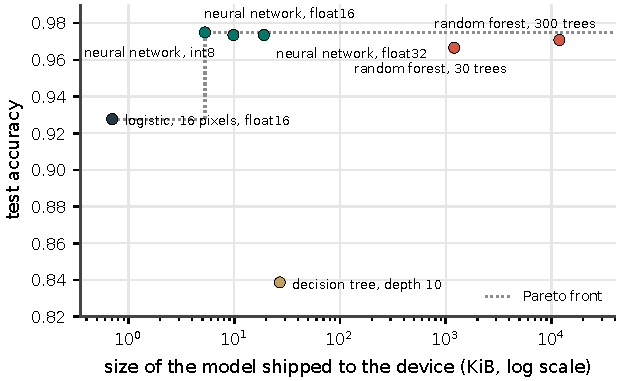
\includegraphics[width=0.78\textwidth]{ch05/on_device}
\caption{Accuracy and size of several models for digit recognition. The dotted line is the Pareto
front: no model is both smaller and more accurate than the models on it.}
\label{fig:ondevice}
\end{figure}

\paragraph{In the browser} Browsers are optimised for fast graphical computation, and libraries such
as TensorFlow.js \citep{smilkov2019tensorflowjs} can train and run most differentiable models in
JavaScript. Users interact with the model without installing anything, and the computation happens on
their devices. The drawback is bandwidth: the model must be downloaded by each visitor (caching helps
when they come back), which again favours small models.

\subsection{Federated learning}

So far we have deployed a single model, trained in advance, for all users. What if each user needed a
different model, as in content recommendation or healthcare? One solution is to give a shared model
user-specific features. Another is \emph{federated learning} \citep{mcmahan2017communication,kairouz2021advances}:
every user has a model with the same architecture but different parameter values; each model learns
from its user's data, and only sends model updates to a server, which aggregates them to improve a
global model and sends it back to the clients (\cref{fig:fedround}). Each user receives a model that
benefits from what all the others have learned, and the data never leave the devices.

\begin{figure}[htbp]
\centering
\begin{tikzpicture}[font=\scriptsize\sffamily,
  srv/.style={draw=edmnavy,fill=edmnavy!8,rounded corners=3pt,minimum width=40mm,minimum height=10mm,align=center},
  dev/.style={draw=edmteal,fill=edmteal!10,rounded corners=4pt,minimum width=23mm,minimum height=12mm,align=center},
  down/.style={-{Stealth[length=1.8mm]},edmnavy,thick},
  up/.style={-{Stealth[length=1.8mm]},edmcoral,thick}]
  \node[srv] (s) at (0,0) {server: $w\leftarrow\sum_k\frac{n_k}{n}\,w_k$\\(4) aggregate the updates};
  \foreach \i/\x in {1/-4.2,2/0,3/4.2} {
    \node[dev] (d\i) at (\x,-2.9) {client \i\\(2) train on its own\\private data};
    \draw[down] ([xshift=-3mm]s.south) ++(0,0) -- ([xshift=-3mm]d\i.north);
    \draw[up] ([xshift=3mm]d\i.north) -- ([xshift=3mm]s.south);
  }
  \node[text=edmnavy,align=right,anchor=east] at (-4.4,-1.25) {(1) the server sends\\the global model $w$};
  \node[text=edmcoral,align=left,anchor=west] at (4.4,-1.25) {(3) each client sends\\back its model $w_k$};
\end{tikzpicture}
\caption{A round of federated averaging: the global model goes down, each client trains it on its
private data and sends it back, and the server averages the local models, weighting each by the
number of examples $n_k$ of its client.}
\label{fig:fedround}
\end{figure}

In \emph{federated averaging} (FedAvg, \citealp{mcmahan2017communication}), the most common algorithm,
each round sends the current global model $w$ to the clients; client $k$ runs a few epochs of
stochastic gradient descent on its $n_k$ examples, obtaining $w_k$; and the server replaces $w$ by the
weighted average $\sum_k(n_k/n)\,w_k$, with $n=\sum_kn_k$. Google's mobile keyboard used federated
learning to improve next-word prediction from the typing of its users without collecting what they
typed \citep{hard2018federated}.

\begin{pylisting}[label={lst:fedavg}]{Federated averaging from scratch, with non-IID clients and personalisation}
import numpy as np
from sklearn.datasets import load_digits
from sklearn.model_selection import train_test_split

rng = np.random.default_rng(0)
X, y = load_digits(return_X_y=True)
X = X / 16.0
X_pool, X_test, y_pool, y_test = train_test_split(X, y, test_size=0.3, random_state=0,
                                                  stratify=y)
K = 10                                             # clients, e.g. phones of 10 users
favourite = (y_pool + rng.integers(0, 2, len(y_pool))) % K   # each digit: 2 clients
to_favourite = rng.random(len(y_pool)) < 0.8                 # 80% go to a favourite
owner = np.where(to_favourite, favourite, rng.integers(0, K, len(y_pool)))
clients = []                                       # non-IID data: (train, own test)
for k in range(K):
    idx = rng.permutation(np.flatnonzero(owner == k))
    cut = int(0.7 * len(idx))
    clients.append((X_pool[idx[:cut]], y_pool[idx[:cut]],
                    X_pool[idx[cut:]], y_pool[idx[cut:]]))

def sgd(W, X, y, epochs, lr=0.5, batch=16):
    """Mini-batch SGD for softmax regression; the last row of W is the bias."""
    W, Xb, Y = W.copy(), np.c_[X, np.ones(len(X))], np.eye(10)[y]
    for _ in range(epochs):
        perm = rng.permutation(len(X))
        for s in range(0, len(X), batch):
            j = perm[s:s + batch]
            Z = Xb[j] @ W
            P = np.exp(Z - Z.max(axis=1, keepdims=True))
            W -= lr * Xb[j].T @ (P / P.sum(axis=1, keepdims=True) - Y[j]) / len(j)
    return W

acc = lambda W, X, y: np.mean(np.argmax(np.c_[X, np.ones(len(X))] @ W, axis=1) == y)
own = lambda models: np.mean([acc(W, c[2], c[3]) for W, c in zip(models, clients)])
W0, n = np.zeros((65, 10)), np.array([len(c[1]) for c in clients])
W, history = W0, []
for rnd in range(30):                              # federated averaging (FedAvg)
    local = [sgd(W, c[0], c[1], epochs=2) for c in clients]      # on the devices
    W = sum(nk * Wk for nk, Wk in zip(n, local)) / n.sum()       # on the server
    history.append(acc(W, X_test, y_test))
central = sgd(W0, np.vstack([c[0] for c in clients]),
              np.concatenate([c[1] for c in clients]), epochs=60)
alone = [sgd(W0, c[0], c[1], epochs=60) for c in clients]
tuned = [sgd(W, c[0], c[1], epochs=2) for c in clients]          # personalisation
print("model                        all digits   each user's own data")
results = {}
for name, models in [("centralised (data pooled)", [central] * K),
                     ("local models only", alone), ("federated averaging", [W] * K),
                     ("federated + fine-tuning", tuned)]:
    everyone = np.mean([acc(m, X_test, y_test) for m in models])
    results[name] = (everyone, own(models))
    print(f"{name:28s}    {everyone:.3f}          {own(models):.3f}")
print(f"each round: {K} clients x {W.size} parameters each way; no data leaves a device")
\end{pylisting}
\begin{pyoutput}
model                        all digits   each user's own data
centralised (data pooled)       0.965          0.969
local models only               0.562          0.874
federated averaging             0.952          0.935
federated + fine-tuning         0.854          0.969
each round: 10 clients x 650 parameters each way; no data leaves a device
\end{pyoutput}

\Cref{lst:fedavg} simulates ten users whose data are \emph{non-IID}, as they are in practice: each user
writes mostly two of the ten digits. A softmax regression is trained in four ways (\cref{fig:federated}).
Pooling all the data on a server, which federated learning forbids, gives an accuracy of 0.965 on all
the digits. A model trained only on each user's data is good at that user's digits (0.874) but poor at
the others (0.562). Federated averaging reaches 0.952 on all the digits after 30 rounds, without any
example leaving its device; and fine-tuning the federated model for two epochs on each device gives
every user a personalised model, and the mean accuracy across clients on their own test data (0.969) matches
that of the centralised model. The mean hides differences: in this run some clients gain and others lose
accuracy with fine-tuning, so the distribution across clients should be reported too. Note that federated
learning concerns how a model is \emph{trained}; the resulting model can then serve predictions on the devices
or on a server.
Personalisation has a cost, though: the fine-tuned models are worse on the digits their users rarely
write (0.854), a trade-off that depends on whether the user's future data will look like their past
data.

\begin{figure}[htbp]
\centering
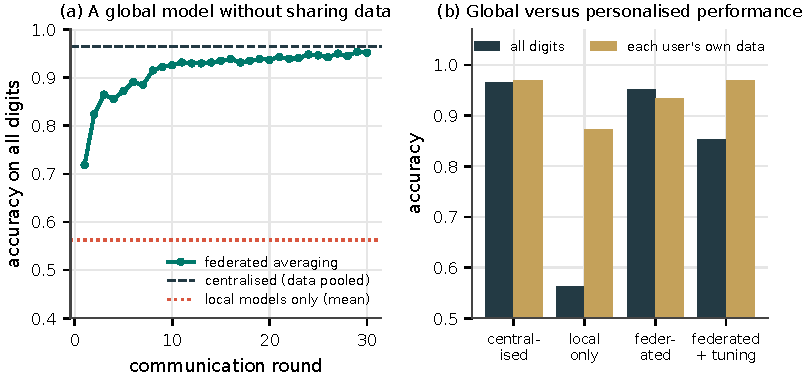
\includegraphics[width=\textwidth]{ch05/federated}
\caption{Federated learning on non-IID digits. (a) Accuracy of the federated model after each
communication round. (b) Accuracy on all the digits and on each user's own data for the four
strategies.}
\label{fig:federated}
\end{figure}

Federated learning is an exciting direction, but it adds a layer of complexity
\citep{li2020federated}: making sure that each individual model performs well, coping with clients
that are slow, offline or malicious, and limiting communication. And keeping the data on the device
is not enough to guarantee privacy, since model updates can leak information about the training
examples \citep{zhu2019deep}; secure aggregation, which lets the server see only the sum of the updates
\citep{bonawitz2017practical}, and differential privacy, which adds calibrated noise
\citep{abadi2016deep}, are used to close that gap.

% =====================================================================
\section{Exchanging and packaging models}\label{sec:exchange}

The environment where a model is trained is often not the one where it runs. A data scientist
trains in Python or R, but the model must score loans inside a Java banking system, rank products in a
database, run on a phone, or answer requests from a service written by another team. There are three
broad ways of moving a trained model from one environment to the other, plus conventions for packaging
it with everything it needs (\cref{tab:formats}).

\begin{table}[htbp]
\centering\small
\caption{Ways of moving a trained model between environments.}\label{tab:formats}
\begin{tabularx}{\textwidth}{@{}>{\raggedright\arraybackslash}p{2.35cm}>{\raggedright\arraybackslash}p{2.6cm}>{\raggedright\arraybackslash}X>{\raggedright\arraybackslash}X@{}}
\toprule
Approach & Examples & Strengths & Weaknesses\\
\midrule
Native serialisation & pickle, joblib, R's \texttt{saveRDS} & trivial; works for any object & same
language and library versions needed; loading an untrusted file can execute arbitrary code\\
Declarative standard & PMML (XML) & readable and auditable; no code execution; engines in Java, R,
databases and analytics platforms & verbose; little support for deep learning or custom
transformations\\
Computation graph standard & ONNX & classical models and deep learning; fast runtimes for servers,
browsers and phones & converters do not cover every model or step; small numerical differences\\
Framework formats & TorchScript, \texttt{torch.export}, TensorFlow SavedModel, LiteRT, Core ML & full
support within one ecosystem; mobile runtimes & tied to that ecosystem\\
Packaging conventions & MLflow Models, BentoML & bundle the model with its environment, signature and a
standard interface & not a format that other runtimes can execute\\
\bottomrule
\end{tabularx}
\end{table}

\subsection{Native serialisation}

The easiest way of saving a scikit-learn model is to serialise the Python object with pickle or joblib,
as R users do with \texttt{saveRDS}. It works for any model, but the file can only be loaded by the same
language, usually with the same versions of the libraries, which ties the production system to the
training environment. Worse, loading a pickle can run arbitrary code, so a pickle from an untrusted
source is a security hole \citep{pythonpickle}. Native serialisation is fine within a team and a
controlled environment, with pinned versions (\cref{sec:infrastructure}); safer formats for scikit-learn
models exist, such as the one of the skops library, which refuses to load unknown types unless the user
trusts them explicitly.

\subsection{PMML}

The \emph{Predictive Model Markup Language} is an XML standard maintained by the Data Mining Group (DMG),
a vendor-neutral consortium, since the late 1990s; its current version is 4.4 \citep{dmg2019pmml,guazzelli2009pmml}.
A PMML document is \emph{declarative}: it describes the model, and an engine that implements the standard
computes the predictions, so loading it never executes code from the author of the file. Its main parts
are:
\begin{itemize}
  \item a \texttt{Header} with information about the producer;
  \item a \texttt{DataDictionary} with the fields of the data: their names, their operational type
        (continuous, categorical or ordinal), their data type (integer, double, string\dots) and their valid
        values;
  \item an optional \texttt{TransformationDictionary} with derived fields (normalisations,
        discretisations, value mappings, arithmetic expressions);
  \item one or more model elements, each with a \texttt{MiningSchema} (which fields it uses, and how to
        treat missing and invalid values), an \texttt{Output} section (which values to return: the
        predicted class, the probabilities\dots), local transformations, and optional
        \texttt{ModelVerification} records, pairs of inputs and expected outputs that the engine checks
        when it loads the model.
\end{itemize}
The standard covers regression and generalised linear models, decision trees, rule sets, naive Bayes,
support vector machines, neural networks, $k$-nearest neighbours, clustering, association rules, sequence
and time series models, and ensembles of any of them through segmentation. PMML documents are produced by
converters for R, Python (sklearn2pmml), Spark, KNIME and commercial tools, and consumed by scoring
engines such as JPMML \citep{jpmml}, by analytics platforms and by some databases.

\begin{pylisting}[label={lst:pmml}]{Exporting a decision tree to PMML and scoring it with an independent Java engine}
import contextlib
import io
import os
import tempfile
import xml.etree.ElementTree as ET
import numpy as np
import pandas as pd
from jpmml_evaluator import make_evaluator
from sklearn.tree import DecisionTreeClassifier
from sklearn2pmml import sklearn2pmml
from sklearn2pmml.pipeline import PMMLPipeline

rng = np.random.default_rng(0)
n = 2000
X = pd.DataFrame({"income": rng.normal(30, 8, n).round(1),
                  "debt_ratio": rng.uniform(0, 0.8, n).round(2),
                  "years_job": rng.integers(0, 30, n)})
logit = -2 + 0.08 * X.income - 3 * X.debt_ratio + 0.03 * X.years_job
y = pd.Series((rng.random(n) < 1 / (1 + np.exp(-logit))).astype(int), name="repays")
tree = DecisionTreeClassifier(max_depth=2, min_samples_leaf=50, random_state=0)
pipe = PMMLPipeline([("tree", tree)]).fit(X, y)
pipe.verify(X.sample(10, random_state=0))       # embed records the engine must reproduce
path = os.path.join(tempfile.mkdtemp(), "loan_tree.pmml")
with contextlib.redirect_stdout(io.StringIO()):            # silence the converter's log
    sklearn2pmml(pipe, path)

# Inside the document: a data dictionary, and the tree as nested nodes with predicates
root = ET.parse(path).getroot()
ns = {"p": root.tag.split("}")[0][1:]}
fields = root.findall("p:DataDictionary/p:DataField", ns)
print(f"PMML {root.get('version')}, {os.path.getsize(path):,} bytes")
print("fields:", ", ".join(f"{f.get('name')} ({f.get('optype')})" for f in fields))

def show(node, depth=0):
    pred = node.find("p:SimplePredicate", ns)
    rule = "root" if depth == 0 else "otherwise" if pred is None else \
        f"{pred.get('field')} {pred.get('operator')} {float(pred.get('value')):.3g}"
    leaf = "" if node.find("p:Node", ns) is not None else f" -> {node.get('score')}"
    print(f"  {'  ' * depth}{rule}{leaf}")
    for child in node.findall("p:Node", ns):
        show(child, depth + 1)

show(root.find("p:TreeModel/p:Node", ns))

# Score the file with an independent engine (Java), which first checks the embedded
# verification records, and compare all the predictions with scikit-learn
print("elements:", [e.tag.split("}")[1] for e in root.find("p:TreeModel", ns)])
scores = make_evaluator(path).verify().evaluateAll(X)
same = np.array_equal(scores["repays"].to_numpy(), pipe.predict(X))
gap = np.abs(scores["probability(1)"].to_numpy() - pipe.predict_proba(X)[:, 1]).max()
print(f"JPMML on {n} applicants: same decisions {same}, largest difference {gap:.1e}")
\end{pylisting}
\begin{pyoutput}
PMML 4.4, 5,064 bytes
fields: repays (categorical), income (continuous), debt_ratio (continuous)
  root
    debt_ratio lessOrEqual 0.275
      income lessOrEqual 27.4 -> 0
      otherwise -> 1
    income lessOrEqual 39.2 -> 0
    otherwise -> 1
elements: ['MiningSchema', 'Output', 'Node', 'ModelVerification']
JPMML on 2000 applicants: same decisions True, largest difference 0.0e+00
\end{pyoutput}

\Cref{lst:pmml} exports a loan model, a decision tree of depth 2, together with ten verification records.
The data dictionary lists only the fields that the model uses: the converter dropped the years in the
job, which the tree ignores. The tree itself is stored as nested nodes, each with a predicate, and an
engine evaluates the children of a node \emph{in order}, following the first whose predicate is true:
a document that a person can read and audit, which links PMML with the interpretable models of
\cref{sec:intmodels}. The JPMML engine, written in Java and independent of scikit-learn, first reproduces
the verification records and then scores the 2000 applicants with exactly the same decisions and
probabilities.

PMML's strengths are its stability, its readability and its safety, which have made it popular in
regulated industries such as banking and insurance, where models must be documented and audited. Its
weaknesses are its verbosity, its limited support for deep learning and for custom preprocessing (a step
that the standard cannot express cannot be exported), and the slow pace at which the standard evolves.
The DMG proposed a more expressive JSON-based successor, the Portable Format for Analytics
\citep{pivarski2016deploying}, but it saw little adoption.

\subsection{ONNX}

The \emph{Open Neural Network Exchange} is a widely used open format for exchanging models.
It was launched in 2017 by Facebook and Microsoft and is now an open-source project of the Linux
Foundation \citep{onnx2019}. An ONNX model is a \emph{computation graph}, stored with Protocol Buffers:
named inputs and outputs, and nodes that apply standard \emph{operators}. Operators belong to versioned
\emph{operator sets} (opsets): the default domain contains the operators of deep learning (convolutions,
matrix products, activations), and the \texttt{ai.onnx.ml} domain the operators of classical machine
learning (scalers, encoders, linear models, tree ensembles). A model declares the opsets it uses, and a
runtime that supports them can execute it.

Converters exist for most frameworks: skl2onnx for scikit-learn, onnxmltools for XGBoost, LightGBM and
Spark, and the exporters of PyTorch and TensorFlow. ONNX Runtime \citep{onnxruntime2021} executes the
models on CPUs and, through \emph{execution providers}, on GPUs and specialised accelerators, as well as
in browsers (with WebAssembly and WebGPU) and on mobile devices; it also includes tools to quantise models
(\cref{lst:ondevice}).

\begin{pylisting}[label={lst:onnx}]{Exporting a pipeline with categorical features to ONNX and comparing latencies}
import time
import numpy as np
import onnxruntime as ort
import pandas as pd
from skl2onnx import to_onnx
from sklearn.compose import ColumnTransformer
from sklearn.ensemble import GradientBoostingClassifier
from sklearn.pipeline import Pipeline
from sklearn.preprocessing import OneHotEncoder, StandardScaler

rng = np.random.default_rng(1)
n = 5000
X = pd.DataFrame({"income": rng.normal(30, 8, n).astype(np.float32),
                  "debt_ratio": rng.uniform(0, 0.8, n).astype(np.float32),
                  "contract": rng.choice(["permanent", "temporary", "self-employed"], n),
                  "region": rng.choice(["north", "south", "east", "west"], n)})
logit = (0.08 * (X.income - 30) - 3 * (X.debt_ratio - 0.4)
         + 0.8 * (X.contract == "permanent") - 0.4)
y = (rng.random(n) < 1 / (1 + np.exp(-logit))).astype(int)
prep = ColumnTransformer([("num", StandardScaler(), ["income", "debt_ratio"]),
                          ("cat", OneHotEncoder(handle_unknown="ignore"),
                           ["contract", "region"])])
pipe = Pipeline([("prep", prep), ("model", GradientBoostingClassifier(random_state=0))])
pipe.fit(X, y)

onx = to_onnx(pipe, X[:1], options={GradientBoostingClassifier: {"zipmap": False}})
print("inputs:", [i.name for i in onx.graph.input])
print("opsets:", {d.domain or "ai.onnx": d.version for d in onx.opset_import})
print("operators:", ", ".join(sorted({node.op_type for node in onx.graph.node})))
session = ort.InferenceSession(onx.SerializeToString(),
                               providers=["CPUExecutionProvider"])
feeds = lambda df: {c: df[[c]].to_numpy() for c in df.columns}   # one input per column
labels, probs = session.run(None, feeds(X))
gap = np.abs(probs[:, 1] - pipe.predict_proba(X)[:, 1]).max()
print(f"same labels: {np.array_equal(labels, pipe.predict(X))}, "
      f"largest probability difference: {gap:.1e}")

def median_ms(f, reps):
    times = []
    for _ in range(reps):
        start = time.perf_counter()
        f()
        times.append(time.perf_counter() - start)
    return 1000 * np.median(times)

one, one_feeds, all_feeds = X[:1], feeds(X[:1]), feeds(X)   # inputs prepared once
sk_one = median_ms(lambda: pipe.predict_proba(one), 300)
ort_one = median_ms(lambda: session.run(None, one_feeds), 300)
print(f"one request: scikit-learn {sk_one:.2f} ms, ONNX Runtime {ort_one:.3f} ms")
sk_all = median_ms(lambda: pipe.predict_proba(X), 10)
ort_all = median_ms(lambda: session.run(None, all_feeds), 10)
print(f"{n} rows:   scikit-learn {sk_all:.1f} ms, ONNX Runtime {ort_all:.1f} ms")
\end{pylisting}
\begin{pyoutput}
inputs: ['income', 'debt_ratio', 'contract', 'region']
opsets: {'ai.onnx': 21, 'ai.onnx.ml': 1}
operators: Concat, Identity, OneHotEncoder, Reshape, Scaler, TreeEnsembleClassifier
same labels: True, largest probability difference: 1.9e-07
one request: scikit-learn 2.57 ms, ONNX Runtime 0.014 ms
5000 rows:   scikit-learn 12.0 ms, ONNX Runtime 12.2 ms
\end{pyoutput}

\Cref{lst:onnx} exports a realistic pipeline: a column transformer that standardises two numeric features
and one-hot encodes two categorical ones, followed by gradient boosting. The ONNX graph has one input per
column, and the operators show how each step was translated: \texttt{Scaler}, \texttt{OneHotEncoder},
\texttt{Concat} and a \texttt{TreeEnsembleClassifier} from the \texttt{ai.onnx.ml} domain. ONNX Runtime
reproduces every label, with probabilities that differ by $2\cdot10^{-7}$ because the exported graph
computes in 32-bit floating point. The latencies tell a story that matters for streaming services
(\cref{lst:latency}): for a single request, ONNX Runtime takes 0.014 ms against 2.6 ms for the
scikit-learn pipeline, almost 200 times less, because it avoids the overhead of the Python objects at every
call; for 5000 rows at once both take about 12 ms, since the work itself dominates. These are microbenchmarks on
prepared inputs: they depend on the hardware, the library versions, the number of threads and the batch
size, and the latency of a service must be measured end to end, under representative load.

Exporting to ONNX has pitfalls of its own. Not every model or transformation has a converter (a custom
Python function in the pipeline, for instance, cannot be translated), the 32-bit arithmetic can change a
decision when a score is very close to a threshold, and the runtime must support the opsets that the model
declares. As with PMML, every export should be checked against the original model on real data, as both
listings do.

\subsection{Framework formats and packaging conventions}

Deep learning frameworks have their own deployment formats: \texttt{torch.export} for PyTorch (TorchScript, its
predecessor, is deprecated and kept for existing systems), the SavedModel format of TensorFlow, LiteRT (formerly TensorFlow Lite) for mobile and embedded
devices, and Core ML for Apple devices. They support most of what their framework can do, within the operators and runtimes available, at the
price of
tying the production system to that ecosystem. \emph{Packaging conventions} solve a different problem.
An MLflow Model \citep{zaharia2018accelerating}, for instance, is a directory that contains the model in
one or several \emph{flavours} (scikit-learn, PyTorch, ONNX\dots), the description of its environment,
a \emph{signature} with the names and types of its inputs and outputs, and a generic Python interface, so
that any MLflow model can be loaded and served in the same way. The choice between all these options
follows from where the model must run, who must read it, and how much the production system can depend on
the training environment.

% =====================================================================
\section{Web applications for models}\label{sec:webapps}

Often the fastest way of putting a model in the hands of its users is a small web application.
\emph{Shiny} \citep{shiny2012} builds interactive applications from code alone: a user interface of input
controls and outputs, and a server function that recomputes the outputs whenever the inputs they depend on
change. Shiny was born in the R community, and Posit, the company that develops it, also maintains Shiny for
Python \citep{shinypython2024}, which we use in this book; \cref{tab:shiny} lists its building blocks. Streamlit
and Gradio play a similar role.

\begin{table}[htbp]
\centering\small
\caption{The building blocks of a Shiny for Python application.}\label{tab:shiny}
\begin{tabular}{@{}ll@{}}
\toprule
Purpose & Shiny for Python\\
\midrule
page layout & \texttt{ui.page\_fluid(...)}, \texttt{ui.page\_sidebar(...)}\\
input control & \texttt{ui.input\_slider("income", ...)}, \texttt{ui.input\_select(...)}\\
place for an output & \texttt{ui.output\_text("answer")}, \texttt{ui.output\_plot(...)}\\
how to build an output & \texttt{@render.text} on a function called \texttt{answer}\\
value of an input & \texttt{input.income()}\\
cached computation & \texttt{@reactive.calc} on a function\\
the application & \texttt{App(app\_ui, server)}\\
running it & \texttt{shiny run app.py}\\
\bottomrule
\end{tabular}
\end{table}

\Cref{lst:loanmodel,lst:shinyapp} build an application that shows the probability that a loan applicant
will repay, given two sliders for the income and the debt ratio. The model is trained beforehand and
loaded when the application starts; the text shown is computed by a small function kept outside the
application, so that it can be tested on its own.

\begin{pylisting}[label={lst:loanmodel}]{The model behind the application, and the answer it shows}
"""The model behind the web application: training, saving and the answer shown."""
from pathlib import Path
import joblib
import numpy as np
import pandas as pd
from sklearn.linear_model import LogisticRegression

PATH = Path(__file__).with_name("loan_model.joblib")

def train_and_save(path=PATH, n=2000, seed=0):
    rng = np.random.default_rng(seed)
    X = pd.DataFrame({"income": rng.normal(30, 8, n), "debt": rng.uniform(0, 1, n)})
    p = 1 / (1 + np.exp(-(0.1 * (X.income - 30) - 2.5 * (X.debt - 0.3) - 0.5)))
    joblib.dump(LogisticRegression().fit(X, (rng.random(n) < p).astype(int)), path)

def answer_text(model, income, debt):
    """The sentence the application shows for an applicant."""
    x = pd.DataFrame({"income": [income], "debt": [debt]})
    return f"Probability of repaying: {model.predict_proba(x)[0, 1]:.2f}"
\end{pylisting}

\begin{pylisting}[label={lst:shinyapp}]{A Shiny for Python application that serves the model}
import joblib
from shiny import App, render, ui
from loan_model import PATH, answer_text

model = joblib.load(PATH)                  # a logistic regression trained beforehand

app_ui = ui.page_fluid(
    ui.panel_title("Loan application"),
    ui.input_slider("income", "Income (thousand EUR)", min=10, max=100, value=30),
    ui.input_slider("debt", "Debt ratio", min=0, max=1, value=0.3, step=0.05),
    ui.output_text("answer"),
)

def server(input, output, session):
    @render.text                           # recomputed whenever an input changes
    def answer():
        return answer_text(model, input.income(), input.debt())

app = App(app_ui, server)                  # run it with: shiny run shiny_app.py
\end{pylisting}

Interactive applications can be tested automatically too (\cref{lst:shinytest}). A unit test checks the
function that builds the answer. The application is an ASGI web application, so a test client can request
its page without starting a server and check that the controls and the output are there. Testing the
\emph{reactivity}, that the answer changes when a slider moves, needs a client that speaks Shiny's
protocol: the browser opens a WebSocket, sends the initial values of the inputs and the outputs it is
showing, receives the computed outputs as JSON messages, and sends updates when the user moves a control.
The test does exactly that, without a browser, and checks that the answer for an income of 80 is the one
the model gives. Tests that drive a real browser, for instance with Playwright, are also possible and check
the rendering as well.

\begin{pylisting}[label={lst:shinytest}]{Testing the application: unit, page and reactivity tests}
import json
import pytest
from starlette.testclient import TestClient
import loan_model

@pytest.fixture(scope="module")
def app_module():
    loan_model.train_and_save()            # the model file that the application loads
    import shiny_app
    return shiny_app

@pytest.fixture(scope="module")
def client(app_module):
    with TestClient(app_module.app) as c:
        yield c

def read_output(ws, name="answer"):
    """Read messages from the server until the value of an output arrives."""
    for _ in range(20):
        message = json.loads(ws.receive_text())
        if name in message.get("values", {}):
            return message["values"][name]
    raise AssertionError(f"output {name} never arrived")

def test_answer_text(app_module):                    # unit test of the model wrapper
    low, high = (loan_model.answer_text(app_module.model, income, 0.3)
                 for income in (20, 80))
    assert low.startswith("Probability of repaying: ")
    assert float(high.split(": ")[1]) > float(low.split(": ")[1])

def test_page_has_the_controls(client):              # the user interface is served
    page = client.get("/")
    assert page.status_code == 200
    assert all(f'id="{name}"' in page.text for name in ("income", "debt", "answer"))

def test_output_follows_the_sliders(client, app_module):   # end to end, no browser
    expected = lambda income: loan_model.answer_text(app_module.model, income, 0.3)
    with client.websocket_connect("/websocket/") as ws:
        ws.send_text(json.dumps({"method": "init", "data": {
            "income": 30, "debt": 0.3, ".clientdata_output_answer_hidden": False}}))
        assert read_output(ws) == expected(30)
        ws.send_text(json.dumps({"method": "update", "data": {"income": 80}}))
        assert read_output(ws) == expected(80)
\end{pylisting}
\begin{pyoutput}
============================= test session starts ==============================
collecting ... collected 3 items

test_shiny_app.py::test_answer_text PASSED                               [ 33%]
test_shiny_app.py::test_page_has_the_controls PASSED                     [ 66%]
test_shiny_app.py::test_output_follows_the_sliders PASSED                [100%]

============================== 3 passed in 1.25s ===============================
\end{pyoutput}

Such applications are ideal for demonstrations, internal tools and prototypes; products with many users need
the architecture of the rest of this unit.

% =====================================================================
\section{Deploying applications built on large language models}\label{sec:llmapps}

A growing share of the models that reach production are not trained by the team that deploys them. An assistant
that answers customers' questions, a tool that extracts fields from contracts or a system that summarises reports
is usually built around a large language model trained by someone else. Deployment then shifts from shipping a
model to shipping everything around it: the instructions it receives, the information it is given, the checks on
what it returns, and the infrastructure that serves it.

\subsection{Where the model runs}

There are three main options. The simplest is an \emph{external API}: no infrastructure, access to the most capable
models, and a price per token processed; but the data leave the organisation, and the provider can change or retire
the model. The second is to \emph{host an open-weight model}, which gives control over the data, the version and the
cost per request, at the price of running GPUs; serving engines batch the requests of many users and manage the memory
of the model carefully to make this efficient \citep{kwon2023efficient}, and the quantisation of
\cref{sec:deployoptions} reduces the hardware needed. The third is to fine-tune a \emph{small model} for one narrow task,
which can be cheaper and faster than a large general one when the task is well defined. The choice involves the same
trade-offs as the options of \cref{sec:deployoptions}, plus one more: whether the data may leave the organisation at all.

\subsection{Prompts are code}

The instructions given to the model, its \emph{prompt}, determine its behaviour as much as the weights of a classical
model determine its predictions. Prompts must therefore be treated like code: kept in templates under version control,
reviewed, tested, and deployed through the same pipeline as everything else (\cref{sec:infrastructure}). A change of a
single sentence in a prompt, or of the version of the model behind an API, is a new release, and it needs the tests and
the cautious rollout of \cref{sec:safedeploy}.

\subsection{Retrieval-augmented generation}

A language model knows only what was in its training data, which is generic, possibly outdated, and does not include the
documents of the organisation. \emph{Retrieval-augmented generation} (RAG) gives it that knowledge at the moment of answering
\citep{lewis2020retrieval}: the documents are split into passages and indexed; for each question, a \emph{retriever} finds the
most relevant passages, and the model is asked to answer using them (\cref{fig:rag}). Knowledge can be updated by updating the
index, without retraining anything; answers can cite their sources; and the documents a user may see can be controlled. But the
answer can be no better than the passages retrieved: if the retriever fails, the model either answers from its general knowledge,
which may be wrong, or invents an answer.

\begin{figure}[htbp]
\centering
\begin{tikzpicture}[font=\scriptsize\sffamily,
  st/.style={draw=edmnavy,fill=edmnavy!6,rounded corners=2pt,minimum height=10mm,minimum width=20mm,align=center},
  gd/.style={draw=edmcoral,fill=edmcoral!12,rounded corners=2pt,minimum height=10mm,minimum width=18mm,align=center},
  arr/.style={-{Stealth[length=1.6mm]},edmnavy}]
  \node[st] (q) at (0,0) {question};
  \node[gd] (g1) at (2.2,0) {input\\guardrails};
  \node[st] (r) at (4.5,0) {retriever};
  \node[st,fill=edmgold!20] (d) at (4.5,-1.6) {index of\\passages};
  \node[st] (p) at (6.9,0) {prompt:\\instructions,\\passages, question};
  \node[st,fill=edmteal!15] (m) at (9.3,0) {language\\model};
  \node[gd] (g2) at (11.5,0) {output\\guardrails};
  \node[st] (a) at (11.5,-1.6) {answer with\\sources, or\\``I don't know''};
  \draw[arr] (q) -- (g1); \draw[arr] (g1) -- (r); \draw[arr] (d) -- (r); \draw[arr] (r) -- (p);
  \draw[arr] (p) -- (m); \draw[arr] (m) -- (g2); \draw[arr] (g2) -- (a);
\end{tikzpicture}
\caption{A retrieval-augmented generation application.}
\label{fig:rag}
\end{figure}

\subsection{Guardrails, tests and security}

\emph{Guardrails} are checks around the model. Before it, they detect personal data that should not be sent, or attempts to
manipulate the assistant; after it, they validate that the output has the expected format (for instance, that it parses as JSON
against a schema), that it is supported by the retrieved passages, and that it contains nothing harmful. One of the most useful
is a guardrail on the retrieval itself: when no passage is relevant enough, the assistant should say that it does not know, an
application of the abstention of \cref{sec:cautious}.

Testing an application whose outputs are free text is harder than testing a classifier, but the principles of
\cref{sec:packaging} still apply. A \emph{test set} of realistic questions, with the passages that answer them and reference answers,
allows the retrieval to be measured with ranking metrics (recall@$k$, the mean reciprocal rank) and the answers to be checked for
correctness and for faithfulness to the passages. Checking free text automatically often uses another language model as a judge,
which agrees reasonably well with human raters but has biases of its own, such as preferring longer answers or the answer
presented first \citep{zheng2023judging}; frameworks package such metrics for RAG \citep{es2024ragas}. Every change of prompt,
model or index should run the test set again in the delivery pipeline, as a regression test.

Language model applications also have specific vulnerabilities \citep{owasp2025llm}. The most characteristic is \emph{prompt
injection}: instructions hidden in the user's message, or in a document or web page that the application retrieves, which the
model may obey \citep{greshake2023not}. Others are the disclosure of sensitive information present in the context and the
\emph{excessive agency} of applications that let a model act (send e-mails, run code, make payments) with more permissions than
the task requires. The defences combine guardrails, the principle of least privilege for every tool the model can use, and human
confirmation of consequential actions.

Finally, every token has a price and a latency. Caching the answers to frequent questions, streaming answers as they are generated,
limiting the length of the context, and \emph{cascades} that try a small, cheap model first and call a large one only when needed
(\cref{sec:cautious}) keep both under control.

\subsection{Measuring the retriever}

\Cref{lst:rag} evaluates the retrieval step of a small assistant for a bank, whose knowledge base has twelve passages, with twelve
questions written as customers would write them, not with the words of the documents. Three lexical retrievers are compared: TF-IDF
on words, TF-IDF on character $n$-grams, which tolerates variations of words, and the average of both.

\begin{pylisting}[label={lst:rag}]{Evaluating the retriever of a RAG application, and when to abstain}
import numpy as np
from sklearn.feature_extraction.text import TfidfVectorizer

DOCS = {   # the knowledge base of a (fictional) bank's assistant
    "card-lost": "If your card is lost or stolen, block it at once in the app or call "
                 "the 24-hour line. A replacement card arrives within five working days.",
    "pin": "You can view the PIN of your card in the app after confirming your "
           "identity. To change it, use any of our cash machines.",
    "limits": "Transfers made in the app are limited to 3,000 euros per day. The limit "
              "can be raised at a branch or with your digital certificate.",
    "abroad": "International transfers outside the euro area take one to three working "
              "days and cost 0.3% of the amount, with a minimum of 6 euros.",
    "overdraft": "An overdraft happens when you spend more than your balance. Overdrawn "
                 "amounts pay 7% annual interest and a one-off fee of 15 euros.",
    "mortgage": "Our fixed-rate mortgage has an APR of 2.9% for up to 30 years and "
                "finances up to 80% of the appraised value of the home.",
    "account": "Opening an account takes ten minutes in the app: you need your identity "
               "document and a selfie. Customers under 25 pay no maintenance fees.",
    "login": "If you cannot log in to the app, update it to the latest version and reset "
             "your access code from the login screen with the code we send by SMS.",
    "savings": "The savings account pays 2% annual interest on balances up to 50,000 "
               "euros, and money can be withdrawn at any time without penalties.",
    "complaints": "Complaints can be filed at any branch, in the app or by post. We "
                  "answer within 15 working days.",
    "phishing": "We never ask for your passwords or codes by phone or e-mail. If you "
                "receive such a message, forward it to our security team.",
    "loan": "Personal loans can be repaid early at any time, with a fee of 1% of the "
            "amount repaid.",
}
QUESTIONS = [("someone stole my wallet with my debit card", "card-lost"),
             ("I forgot the secret number of my card", "pin"),
             ("how much money can I send per day from my phone", "limits"),
             ("what does it cost to send money to the United States", "abroad"),
             ("what happens if my balance goes negative", "overdraft"),
             ("which interest rate do you offer for buying a house", "mortgage"),
             ("what do I need to become a customer", "account"),
             ("the application does not let me sign in", "login"),
             ("how much do I earn if I keep my money with you", "savings"),
             ("I want to complain about a charge", "complaints"),
             ("I got an email asking for my password, is it you?", "phishing"),
             ("can I pay back my loan before the end", "loan")]
OUT_OF_SCOPE = ["what will the weather be like tomorrow", "recommend me a good film"]
ids, texts = list(DOCS), list(DOCS.values())
questions, truth = [q for q, _ in QUESTIONS], [ids.index(d) for _, d in QUESTIONS]

def similarities(vectorizer, queries):
    D = vectorizer.fit_transform(texts)
    return (vectorizer.transform(queries) @ D.T).toarray()   # cosine (rows normalised)

words = TfidfVectorizer(stop_words="english")
chars = TfidfVectorizer(analyzer="char_wb", ngram_range=(3, 5))
retrievers = {"words": lambda q: similarities(words, q),
              "character n-grams": lambda q: similarities(chars, q),
              "both (average)": lambda q: (similarities(words, q)
                                           + similarities(chars, q)) / 2}
print("retriever            recall@1  recall@3  mean reciprocal rank")
for name, retrieve in retrievers.items():
    rank = np.array([list(np.argsort(-s)).index(t) + 1
                     for s, t in zip(retrieve(questions), truth)])
    print(f"{name:20s} {np.mean(rank == 1):8.2f}  {np.mean(rank <= 3):8.2f}  "
          f"{np.mean(1 / rank):10.2f}")

S = retrievers["both (average)"](questions + OUT_OF_SCOPE)
best = S.max(axis=1)
print(f"best score: in-scope questions {best[:12].min():.2f} to {best[:12].max():.2f}, "
      f"out of scope {best[12:].min():.2f} to {best[12:].max():.2f}")
for q, s, t in zip(questions, S, truth):
    if s.argmax() != t:                      # the top passage is not the right one
        print(f"  top-1 miss: '{q}' -> {ids[s.argmax()]}")
\end{pylisting}
\begin{pyoutput}
retriever            recall@1  recall@3  mean reciprocal rank
words                    0.58      0.67        0.66
character n-grams        0.67      0.92        0.78
both (average)           0.67      0.92        0.78
best score: in-scope questions 0.09 to 0.42, out of scope 0.05 to 0.07
  top-1 miss: 'I forgot the secret number of my card' -> card-lost
  top-1 miss: 'how much money can I send per day from my phone' -> phishing
  top-1 miss: 'what does it cost to send money to the United States' -> login
  top-1 miss: 'can I pay back my loan before the end' -> overdraft
\end{pyoutput}

Retrieval on words puts the right passage first for only 58\% of the questions; character $n$-grams and the combination reach 67\%,
and find the right passage among the first three for 92\% of them, with a mean reciprocal rank of 0.78. The failures share a cause:
the question and the passage use different words for the same thing (``secret number'' and ``PIN'', ``send money'' and
``transfer'', ``pay back'' and ``repaid''). This is why production systems use \emph{dense} retrievers, which compare embeddings
learned to place paraphrases close together, often combined with lexical retrieval. The last lines show the abstention guardrail at
work: questions outside the scope of the bank score at most 0.07, while the in-scope questions score at least 0.09, so a threshold
between them lets the assistant decline questions it cannot answer. The margin is narrow, and a threshold chosen on twelve questions
must be validated on many more and monitored once the assistant is in use (\cref{sec:llmmonitor}).

% =====================================================================
\section{Creating a development infrastructure}\label{sec:infrastructure}

The goal of a data science project is to create a product that helps real people. Often this means a
stable piece of software that operates in production under a heavy load, and any data science product
is also a software product. Teams can therefore borrow the best practices of software development to
avoid many pitfalls, but they also need some practices of their own, because machine learning systems
depend on data as much as on code and accumulate their own kind of technical debt
\citep{sculley2015hidden,amershi2019software}.

\subsection{From DevOps to ModelOps}

\emph{ModelOps} is a set of practices for automating the operations that recur in data science
projects: the model training pipeline, data management, version control, experiment tracking, testing
and deployment \citep{dubovikov2019managing}; the broader term \emph{MLOps} is now more common
\citep{kreuzberger2023mlops}. Each of these tasks is easy in itself, but without automation teams waste
time repeating them and projects suffer from the mistakes made along the way. The aim is to make
projects reliable, experiments reproducible and deployments fast.

Its closest relative is \emph{DevOps} (development operations), the set of activities that take
software from its source code to a working product: checking the code for errors (typos, bad
practices), building it for one or several target platforms, running tests that check that it works as
required, packaging it and deploying the package. These steps are repetitive and error-prone, and
\emph{continuous integration and continuous delivery} (CI/CD) states that they can and should be
automated and run as often as possible \citep{humble2010continuous}: small, thoroughly tested updates
are more reliable than large ones, and easier to revert. Once a change is pushed, a CI/CD server
(Jenkins, GitLab CI/CD, GitHub Actions, Travis CI or CircleCI) launches the delivery pipeline. Writing
automated tests and defining the pipelines takes time, but afterwards the pipeline just works. CI/CD
servers have become powerful enough to need specialists, the DevOps engineers, but many tools now take
only a few clicks to set up, and most of their benefits apply to data science projects.

The usual DevOps infrastructure has four components: version control (Git), a code collaboration
platform (GitHub, GitLab), an automated testing framework for the language of the project, and a CI/CD
server. It misses three features that are critical for data science:
\begin{itemize}
  \item \emph{data management}: storing and versioning large data files;
  \item \emph{experiment tracking}: recording the results of many experiments and the code and data that
        produced them;
  \item \emph{automated testing of data-heavy applications}, whose behaviour depends on data and whose
        complete pipelines can run for hours.
\end{itemize}
A useful checklist of what a production machine learning system should test and monitor is the
\emph{ML test score} of \citet{breck2017ml}.

\subsection{The data science delivery pipeline}

The code of a data science project can be structured as a set of pipelines
(\cref{fig:delivery}). Every model starts from \emph{raw data}. Data scientists explore it and produce
EDA reports; a \emph{data processing pipeline} transforms the raw data into an intermediate, cleaned
format; a \emph{model dataset pipeline} creates the data sets for training, validating and testing
models; and a \emph{model training pipeline} uses them to train, validate and test models, producing
quality reports and, at the end, the final trained model. Each intermediate result is a branching
point from which several pipelines can start: from one cleaned data set we can build several model
data sets without rerunning the cleaning each time.

\begin{figure}[htbp]
\centering
\begin{tikzpicture}[font=\scriptsize\sffamily,
  pl/.style={draw=edmteal,fill=edmteal!10,rounded corners=2pt,minimum height=9mm,minimum width=17mm,align=center},
  ds/.style={cylinder,shape border rotate=90,draw=edmnavy,fill=edmbronze!25,aspect=0.25,minimum width=13mm,minimum height=9mm,align=center},
  doc/.style={draw=edmnavy,fill=white,minimum width=14mm,minimum height=7mm,align=center},
  arr/.style={-{Stealth[length=1.6mm]},edmnavy}]
  \node[ds] (raw) at (0,0) {raw\\data};
  \node[pl] (eda) at (1.9,1.25) {EDA};
  \node[doc] (rep) at (3.9,1.25) {EDA\\reports};
  \node[pl] (proc) at (2.05,0) {data\\processing};
  \node[ds] (clean) at (4.0,0) {cleaned\\data};
  \node[pl] (mds) at (6.0,0) {model data\\sets};
  \node[ds] (sets) at (8.0,0) {train, valid.\\and test};
  \node[pl] (train) at (10.0,0) {model\\training};
  \node[ds] (model) at (12.0,0) {trained\\model};
  \node[doc] (qual) at (10.0,1.25) {quality\\reports};
  \draw[arr] (raw) |- (eda);
  \draw[arr] (eda) -- (rep);
  \foreach \a/\b in {raw/proc,proc/clean,clean/mds,mds/sets,sets/train,train/model} \draw[arr] (\a) -- (\b);
  \draw[arr] (train) -- (qual);
  \draw[decorate,decoration={brace,mirror,amplitude=4pt},edmbronze] (-0.6,-0.85) -- (12.6,-0.85)
    node[midway,below=5pt,text=edmbronze,align=center] {data artefacts (cylinders) are versioned with DVC,
    code (rounded boxes) with Git};
\end{tikzpicture}
\caption{The data science delivery pipeline: each pipeline is code that turns one data artefact into
the next.}
\label{fig:delivery}
\end{figure}

\subsection{Managing code versions and quality}

Source version control with Git is a mandatory component of any data science project, and platforms
such as GitHub and GitLab provide ready-to-use Git servers, tools for code review and issue management,
and integration with CI/CD \citep{chacon2014pro}. A branching model, such as GitFlow
\citep{driessen2010successful}, gives the whole team the same rules for creating features, releases and
fixes. Python, the language of most data science projects, has a weaker tradition of static code
analysis than compiled languages, but it has the tools: style checkers (Flake8 and its extensions),
static type checking (MyPy), and pre-commit, which runs these checks automatically before every commit.

\subsection{Versioning data}

Different versions of the code of a data science project produce different outputs, and to reproduce
or reuse them we must be able to recover the exact data each version used. A software product can be
rebuilt from its source code alone; a data science product cannot. We should therefore version the data
along with the code, and store and document not only the incoming data but also the intermediate data
sets, which saves recomputing them (at the price of disk space).

Git is ill suited to data. It records snapshots of the project as content-addressed objects (and may compress
similar objects with deltas), which is perfect for source code; but every version of a large data file that
changes often adds another large object, making repositories slow to clone and to maintain. For data it is simpler to store the entire file each time it changes. Git LFS (large file storage)
keeps large files outside the repository and stores only pointers to them. \emph{DVC} (data version
control, \citealp{dvc2024}) goes further: it identifies each data file by a hash of its contents, keeps
small metafiles with those hashes in Git, stores the data themselves in remote storage (a server, a
cloud bucket), and describes pipelines as graphs of stages with their commands, inputs and outputs
(\cref{lst:dvc}). With \texttt{dvc repro}, DVC reruns only the stages whose declared dependencies, parameters or outputs have
changed, reusing cached results otherwise, so
anyone can rebuild any version of the results with a single command.

\begin{pylisting}[label={lst:dvc},listing options={style=outstyle}]{A two-stage DVC pipeline (dvc.yaml)}
stages:
  prepare:
    cmd: python src/prepare.py data/raw.csv data/clean.parquet
    deps:
      - src/prepare.py
      - data/raw.csv
    outs:
      - data/clean.parquet
  train:
    cmd: python src/train.py data/clean.parquet models/model.pkl
    deps:
      - src/train.py
      - data/clean.parquet
    params:
      - train.n_estimators          # read from params.yaml, tracked as well
    outs:
      - models/model.pkl
    metrics:
      - reports/metrics.json:
          cache: false
\end{pylisting}

\subsection{Managing environments}

Data science projects depend on many open-source libraries that change frequently, sometimes breaking
their interfaces. All the dependencies must be fixed in a shareable format, so that every member of the
team, and every server, uses the same versions. In Python, pyenv manages several Python installations on
one machine; virtualenv (or the built-in venv) creates isolated environments with different sets of
packages; pipenv, Poetry and similar tools create shareable environments with a lock file that pins every
version. Conda is particularly popular in data science: it shares environments through an
\texttt{environment.yml} file, provides the Anaconda distribution with many data science packages
preinstalled and optimised, and installs non-Python dependencies such as the CUDA libraries needed to run
deep networks on GPUs. Containers (\cref{sec:packaging}) isolate even more: the processes and the user space of the operating
system, while sharing the kernel of the host.

\subsection{Tracking experiments}

Data scientists run many experiments: with features, with algorithms, with hyperparameters. Each must be
reproducible in isolation, because results influence each other, and all the results must be recorded so
that the team can compare variants and choose the best by its metrics. A simple file is enough to start: a
spreadsheet or a CSV file, versioned in Git with the code, with one row per experiment and, at least, the
columns of \cref{tab:tracking}.

\begin{table}[htbp]
\centering\small
\caption{A minimum set of columns for an experiment log.}\label{tab:tracking}
\begin{tabularx}{\textwidth}{@{}lX@{}}
\toprule
Column & Content\\
\midrule
date, description & when the experiment was run, and what it tried\\
code version & the Git commit of the code\\
model, parameters & the algorithm and all its hyperparameters\\
training data & size and link (or hash) of the training set\\
validation data & size and link, or the number of folds for cross-validation\\
test data & size and link of the test set\\
metrics & one column per metric and data set\\
outputs & links to the trained model and other output files\\
\bottomrule
\end{tabularx}
\end{table}

\begin{pylisting}[label={lst:tracking}]{A file-based experiment log with fingerprints of the code and the data}
import csv
import datetime
import hashlib
import json
import os
import subprocess
import tempfile
import numpy as np
import pandas as pd
from sklearn.datasets import make_classification
from sklearn.ensemble import RandomForestClassifier
from sklearn.linear_model import LogisticRegression
from sklearn.model_selection import cross_val_score, train_test_split

LOG = os.path.join(tempfile.mkdtemp(), "experiments.csv")   # versioned with the code
COLUMNS = ["date", "code_version", "model", "params", "train_size", "train_data",
           "test_size", "test_data", "cv_accuracy", "test_accuracy", "description"]

def fingerprint(*arrays):
    """Content hash of a data set (as DVC does): any change gives a new version."""
    h = hashlib.sha256()
    for a in arrays:
        h.update(np.ascontiguousarray(a).tobytes())
    return h.hexdigest()[:10]

def code_version():
    """Git commit of the code; outside a repository, a hash of this file."""
    try:
        cmd = ["git", "rev-parse", "--short", "HEAD"]
        return subprocess.check_output(cmd, stderr=subprocess.DEVNULL, text=True).strip()
    except (OSError, subprocess.CalledProcessError):
        return hashlib.sha256(open(__file__, "rb").read()).hexdigest()[:7]

def log_experiment(row):
    new = not os.path.exists(LOG)
    with open(LOG, "a", newline="") as fh:
        writer = csv.DictWriter(fh, COLUMNS)
        if new:
            writer.writeheader()
        writer.writerow(row)

X, y = make_classification(n_samples=2000, n_features=20, n_informative=6, random_state=3)
X_tr, X_te, y_tr, y_te = train_test_split(X, y, test_size=0.3, random_state=0)
for Model, params, description in [
        (LogisticRegression, {"C": 0.1}, "baseline"),
        (LogisticRegression, {"C": 10.0}, "less regularisation"),
        (RandomForestClassifier, {"n_estimators": 200, "random_state": 0}, "non-linear")]:
    m = Model(**params)
    log_experiment(dict(
        date=datetime.date.today().isoformat(), code_version=code_version(),
        model=Model.__name__, params=json.dumps(params), description=description,
        train_size=len(y_tr), train_data=fingerprint(X_tr, y_tr),
        test_size=len(y_te), test_data=fingerprint(X_te, y_te),
        cv_accuracy=round(cross_val_score(m, X_tr, y_tr, cv=5).mean(), 4),
        test_accuracy=round(m.fit(X_tr, y_tr).score(X_te, y_te), 4)))

log = pd.read_csv(LOG)
table = log[["model", "params", "cv_accuracy", "test_accuracy"]]
table = table.rename(columns={"cv_accuracy": "cv", "test_accuracy": "test"})
print(table.to_string(index=False))
print(f"code version {log.code_version[0]}, training data {log.train_data[0]}")
X_tr[0, 0] += 1e-9                                   # change one value of the data...
print(f"after changing one value: training data {fingerprint(X_tr, y_tr)}")
\end{pylisting}
\begin{pyoutput}
                 model                                   params     cv   test
    LogisticRegression                               {"C": 0.1} 0.8514 0.8617
    LogisticRegression                              {"C": 10.0} 0.8529 0.8600
RandomForestClassifier {"n_estimators": 200, "random_state": 0} 0.9200 0.9267
code version 887dcf3, training data d83a2cc41c
after changing one value: training data ddb8b87ecb
\end{pyoutput}

\Cref{lst:tracking} implements such a log. Each experiment records a \emph{fingerprint} of the data, a hash
of its contents like those of DVC, so that changing a single value by $10^{-9}$ produces a different
fingerprint and the log can never silently mix results obtained on different data. When the team and the
number of experiments grow, a file becomes cumbersome, and three open-source tools are popular, which are
not mutually exclusive: \emph{Sacred} \citep{greff2017sacred}, a feature-packed tracker that records a wide
range of information (metrics, artefacts, logs, even the source code and the machine), locally through
file-based observers or in shared storage such as MongoDB; \emph{MLflow} \citep{zaharia2018accelerating}, easy to integrate, usable locally or with a
shared server, which also packages projects and serves models through an API; and \emph{DVC}, whose
experiment tracking is basic but whose fully versioned, reproducible pipelines let any team member pull
code, data and pipelines and reproduce a result with one command.

The fingerprint identifies the content of the data in this example; it is not a complete record of
provenance. A reproducible experiment also needs the schema of the data, a full digest and the data
themselves, the code actually executed (including uncommitted changes), the effective parameters, the
split, the seeds, the environment and the resulting artefacts.

\subsection{Automated testing}

Small changes in one part of a program can break another. Automated tests, written in a programming
language, check that everything still works as often as we like, typically at every change; large projects
have thousands of them, which CI servers run in parallel. Tests form a hierarchy (\cref{fig:pyramid}):
\emph{unit tests} check individual functions and classes, such as a preprocessing method; \emph{integration
tests} check that the components work together, for instance that all the steps of a pipeline finish
successfully on a small sample; and \emph{end-to-end tests} check a major function of the whole system, such
as training a model on the full data set.

\begin{figure}[htbp]
\centering
\begin{tikzpicture}[font=\scriptsize\sffamily]
  \fill[edmcoral!25] (-1.2,2.0) -- (1.2,2.0) -- (0,3.0) -- cycle;
  \fill[edmgold!35] (-2.4,1.0) -- (2.4,1.0) -- (1.2,2.0) -- (-1.2,2.0) -- cycle;
  \fill[edmteal!25] (-3.6,0) -- (3.6,0) -- (2.4,1.0) -- (-2.4,1.0) -- cycle;
  \draw[edmnavy] (-3.6,0) -- (3.6,0) -- (0,3.0) -- cycle;
  \draw[edmnavy] (-2.4,1.0) -- (2.4,1.0);
  \draw[edmnavy] (-1.2,2.0) -- (1.2,2.0);
  \node at (0,2.35) {end-to-end};
  \node at (0,1.45) {integration};
  \node at (0,0.45) {unit};
  \node[anchor=west,align=left,text=edmnavy] at (3.9,2.4) {few, slow, expensive:\\train on the full data};
  \node[anchor=west,align=left,text=edmnavy] at (3.9,1.45) {the pipeline runs\\on a sample};
  \node[anchor=west,align=left,text=edmnavy] at (3.9,0.45) {many, fast:\\one function each};
\end{tikzpicture}
\caption{The test pyramid of a data science project.}
\label{fig:pyramid}
\end{figure}

Testing data science code is harder than testing ordinary software, because behaviour depends on data:
a complete test of a training pipeline may need gigabytes of data and hours or days of computation on a
cluster. Ignoring tests, however, turns out to be much more expensive than writing them, and their
benefits grow with the size and complexity of the project and of the team. If the pipeline is split into
steps with clearly defined interfaces, each step can be tested separately, for instance the preprocessing
apart from the training. The guidelines are simple: architect the code for testability, start small with
unit tests, consider integration and end-to-end tests, and keep at it. Besides tests of the code, data
science projects need tests of the \emph{data} (schemas, ranges, distributions) and of the \emph{models}:
a minimum performance with respect to a simple baseline, \emph{invariance} tests (the prediction must not
change when an irrelevant attribute changes) and \emph{directional expectation} tests (the prediction must
move in a known direction when a feature does), ideas borrowed from behavioural testing
\citep{ribeiro2020beyond}. \emph{Property-based testing}, with libraries such as Hypothesis
\citep{maciver2019hypothesis}, generates hundreds of random inputs to check that a property always holds.

\begin{pylisting}[label={lst:pipelinelib}]{A small credit-scoring pipeline written to be tested}
"""A small credit-scoring pipeline, written so that it can be tested (Unit 5)."""
import numpy as np
import pandas as pd
from sklearn.impute import SimpleImputer
from sklearn.linear_model import LogisticRegression
from sklearn.pipeline import make_pipeline
from sklearn.preprocessing import FunctionTransformer

FEATURES = ["age", "income", "debt"]

def clip_age(df):
    """A fixed rule, the same for every batch: keep the features, clip the ages."""
    out = df[FEATURES].copy()
    out["age"] = out["age"].clip(18, 100)
    return out

def validate(df):
    """Data quality checks on schema, values and ranges; returns the problems found."""
    problems = [f"missing column {c}" for c in FEATURES if c not in df]
    if problems:
        return problems
    X = df[FEATURES]
    if not all(pd.api.types.is_numeric_dtype(X[c]) for c in FEATURES):
        return ["non-numeric values"]
    if np.isinf(X.to_numpy(dtype=float)).any():
        problems.append("infinite values")
    if (X["income"] < 0).any():
        problems.append("negative income")
    if (X["debt"] < 0).any():
        problems.append("negative debt")
    return problems

def train(df, y):
    """Fixed cleaning, a median imputation learned on the training data only and the
    classifier, in one pipeline saved and reused unchanged for every prediction."""
    model = make_pipeline(FunctionTransformer(clip_age),
                          SimpleImputer(strategy="median", keep_empty_features=True),
                          LogisticRegression(max_iter=1000))
    return model.fit(df, y)

def make_data(n=1000, seed=0):
    rng = np.random.default_rng(seed)
    df = pd.DataFrame({"name": [f"client{i}" for i in range(n)],
                       "age": rng.integers(18, 80, n), "income": rng.normal(30, 8, n),
                       "debt": rng.uniform(0, 20, n)})
    logit = 0.15 * (df.income - 30) - 0.2 * (df.debt - 10)
    return df, (rng.random(n) < 1 / (1 + np.exp(-logit))).astype(int)
\end{pylisting}

\begin{pylisting}[label={lst:tests}]{Eight automated tests for the pipeline, run with pytest}
import numpy as np
import pandas as pd
from hypothesis import given, strategies as st
from pipeline_lib import FEATURES, clip_age, make_data, train, validate

MODEL = train(*make_data(500))

def test_clip_age():                                         # unit test
    df = pd.DataFrame({"age": [10, 50, 130], "income": [20.0, None, 40.0], "debt": 1.0})
    assert clip_age(df)["age"].tolist() == [18, 50, 100]

def test_imputation_learned_once():                         # unit test: no batch effects
    alone = pd.DataFrame({"age": [40], "income": [np.nan], "debt": [5.0]})
    others = pd.DataFrame({"age": [30, 50], "income": [100.0, 200.0],
                           "debt": [1.0, 2.0]})
    p_alone = MODEL.predict_proba(alone)[0, 1]
    p_batch = MODEL.predict_proba(pd.concat([alone, others]))[0, 1]
    assert np.isclose(p_alone, p_batch)
    df, _ = make_data(500)
    imputer = MODEL.named_steps["simpleimputer"]
    assert np.isclose(imputer.statistics_[1], df.income.median())

rows = st.lists(st.tuples(st.integers(-50, 200), st.none() | st.floats(0, 1e6),
                          st.floats(0, 50)), min_size=1, max_size=50)

@given(rows)
def test_predictions_are_probabilities(rows):               # property-based test
    p = MODEL.predict_proba(pd.DataFrame(rows, columns=FEATURES))[:, 1]
    assert np.isfinite(p).all() and ((p >= 0) & (p <= 1)).all()

def test_validate_detects_bad_data():                       # data validation
    df, _ = make_data(50)
    assert validate(df) == []
    assert validate(df.assign(income=-df.income.abs())) == ["negative income"]
    assert validate(df.assign(debt=np.inf)) == ["infinite values"]
    assert validate(df.drop(columns="debt")) == ["missing column debt"]

def test_model_beats_baseline():                            # model quality
    df, y = make_data(2000)
    model = train(df[:1500], y[:1500])
    accuracy = model.score(df[1500:], y[1500:])
    assert accuracy > max(y[1500:].mean(), 1 - y[1500:].mean()) + 0.05

def test_invariance_to_identifiers():                       # invariance test
    df, _ = make_data(500)
    renamed = df.assign(name="someone else")
    assert np.allclose(MODEL.predict_proba(df), MODEL.predict_proba(renamed))

def test_more_income_never_hurts():                         # directional expectation
    x = make_data(100)[0]
    richer = x.assign(income=x.income + 10)
    assert (MODEL.predict_proba(richer)[:, 1] >= MODEL.predict_proba(x)[:, 1]).all()

def test_pipeline_end_to_end():                             # integration test
    df, y = make_data(300, seed=1)
    df.loc[::10, "income"] = None                           # missing values in new data
    assert validate(df) == []
    predictions = train(df, y).predict(df)
    assert len(predictions) == len(df) and set(predictions) <= {0, 1}
\end{pylisting}
\begin{pyoutput}
============================= test session starts ==============================
collecting ... collected 8 items

test_pipeline.py::test_clip_age PASSED                                   [ 12%]
test_pipeline.py::test_imputation_learned_once PASSED                    [ 25%]
test_pipeline.py::test_predictions_are_probabilities PASSED              [ 37%]
test_pipeline.py::test_validate_detects_bad_data PASSED                  [ 50%]
test_pipeline.py::test_model_beats_baseline PASSED                       [ 62%]
test_pipeline.py::test_invariance_to_identifiers PASSED                  [ 75%]
test_pipeline.py::test_more_income_never_hurts PASSED                    [ 87%]
test_pipeline.py::test_pipeline_end_to_end PASSED                        [100%]

============================== 8 passed in 2.06s ===============================
\end{pyoutput}

\Cref{lst:pipelinelib,lst:tests} show a small credit-scoring pipeline and eight tests run with pytest. The
pipeline separates a fixed cleaning rule (clipping the ages) from a transformation learned from data (the
median used to impute missing incomes), which is learned on the training data only and saved with the
model, so that a request receives the same answer alone or in a batch. The tests are: a unit test of the
cleaning rule; a unit test that the imputation does not depend on the batch; a property-based test that,
for random tables of ages, incomes and debts, the predictions are always valid probabilities; a data
validation test of schema, finite values and ranges; a test that the model beats the
majority-class baseline by five points; an invariance test that guards against identifiers leaking into
the features; a directional test that a higher income never lowers the predicted probability of
repaying; and an integration test of the whole pipeline on a sample with missing values.

\subsection{Packaging code}\label{sec:packaging}

There are three ways of deploying Python code. \emph{Plain scripts} copied to the server are the simplest,
but they need a lot of manual preparation (installing every package, filling in configuration files) and
are not recommended. \emph{Python packages}, defined with a \texttt{pyproject.toml} or \texttt{setup.py}
file, are much more convenient, and tools such as PyScaffold provide templates. \emph{Docker images}
\citep{merkel2014docker} package the code with all its dependencies, including the Python interpreter, data
files and an operating system distribution, into an isolated, portable environment that runs on any Linux
machine without the weight of a virtual machine. An image is built from the instructions of a
\emph{Dockerfile} (\cref{lst:dockerfile}); a running instance of an image is a \emph{container}.
Kubernetes orchestrates containers at scale, automating their deployment, scaling and management
\citep{burns2016borg}, and configuration management tools such as Ansible automate deployments that do not
use containers.

\begin{pylisting}[label={lst:dockerfile},listing options={style=outstyle}]{A Dockerfile for the prediction service}
FROM python:3.12-slim
WORKDIR /app
COPY requirements.txt .
RUN pip install --no-cache-dir -r requirements.txt   # pinned versions
COPY src/ ./src/
COPY models/model.onnx ./models/
EXPOSE 8000
CMD ["gunicorn", "--bind", "0.0.0.0:8000", "--workers", "4", "src.api:app"]
\end{pylisting}

\subsection{Continuous model training}

The goal of applying CI/CD to data science is a \emph{continuous training} pipeline that produces new model
versions automatically, so that the team can examine the results of an experiment right after pushing a
change and, if the automated tests pass and the quality reports are good, deploy the model to an online
test environment. The pipeline has three parts (\cref{fig:cicd}): continuous integration (static code
analysis and automated tests); continuous model training (fetch new data, generate EDA reports, run data
quality tests, process the data and create the training set, train a new model, test its quality, and
record the results in the experiment log); and continuous delivery (package the model and the code, publish
them to the target server, and launch the new version). The CI/CD parts are what CI/CD servers were made
for, and continuous training is not hard either, as long as the pipeline can be launched from the command
line, for instance with \texttt{dvc repro}. \Cref{lst:gitlabci} sketches such a pipeline for GitLab CI/CD.

\begin{figure}[htbp]
\centering
\begin{tikzpicture}[font=\scriptsize\sffamily,
  st/.style={draw=edmnavy,fill=edmnavy!6,rounded corners=2pt,minimum height=8mm,minimum width=15mm,align=center},
  lane/.style={draw=#1,fill=#1!7,rounded corners=4pt},
  lab/.style={anchor=east,align=right,font=\scriptsize\sffamily\bfseries},
  arr/.style={-{Stealth[length=1.6mm]},edmnavy}]
  \draw[lane=edmindigo] (-0.9,0.55) rectangle (2.7,-0.65);
  \node[lab,text=edmindigo] at (-1.0,-0.05) {CI};
  \node[st] (c1) at (0,-0.05) {static\\analysis};
  \node[st] (c2) at (1.8,-0.05) {automated\\tests};
  \draw[lane=edmteal] (-0.9,-0.95) rectangle (11.7,-2.15);
  \node[lab,text=edmteal] at (-1.0,-1.55) {continuous\\training};
  \foreach \i/\t in {0/fetch new\\data,1/EDA\\reports,2/data quality\\tests,3/build the\\training set,4/train a\\new model,5/test its\\quality,6/log the\\experiment}
    \node[st] (t\i) at ({\i*1.8},-1.55) {\t};
  \foreach \i [evaluate=\i as \j using int(\i+1)] in {0,...,5} \draw[arr] (t\i) -- (t\j);
  \draw[lane=edmcoral] (-0.9,-2.45) rectangle (6.3,-3.65);
  \node[lab,text=edmcoral] at (-1.0,-3.05) {CD};
  \foreach \i/\t in {0/package\\the model,1/package\\the code,2/publish to\\the server,3/launch the\\new version}
    \node[st] (d\i) at ({\i*1.8},-3.05) {\t};
  \foreach \i [evaluate=\i as \j using int(\i+1)] in {0,...,2} \draw[arr] (d\i) -- (d\j);
  \draw[arr] (c1) -- (c2);
  \draw[arr] (c2.south) -- ++(0,-0.15) -| (t0.north);
  \draw[arr] (t6.south) -- ++(0,-0.3) -| (d0.north);
\end{tikzpicture}
\caption{Continuous integration, continuous model training and continuous delivery.}
\label{fig:cicd}
\end{figure}

\begin{pylisting}[label={lst:gitlabci},listing options={style=outstyle}]{A GitLab CI/CD pipeline for continuous training (.gitlab-ci.yml)}
stages: [check, test, train, package, deploy]

lint:
  stage: check
  script: [pre-commit run --all-files]

unit-tests:
  stage: test
  script: [pytest tests/]

train-model:
  stage: train
  script:
    - dvc pull              # data and cached results of earlier runs
    - dvc repro             # rerun only the stages whose inputs changed
    - python scripts/quality_gate.py reports/metrics.json
  artifacts:
    paths: [models/, reports/]

build-image:
  stage: package
  script:
    - docker build -t $CI_REGISTRY_IMAGE:$CI_COMMIT_SHORT_SHA .
    - docker push $CI_REGISTRY_IMAGE:$CI_COMMIT_SHORT_SHA

deploy-production:
  stage: deploy
  when: manual              # a person approves the release
  script: [./deploy.sh $CI_COMMIT_SHORT_SHA]
\end{pylisting}

\begin{pylisting}[label={lst:ct}]{Continuous training under drift, with a data test and a quality gate}
import numpy as np
from sklearn.linear_model import LogisticRegression

rng = np.random.default_rng(4)

def week_data(t, n=2000):
    """Data of week t: the true decision boundary rotates slowly (concept drift)."""
    X = rng.normal(size=(n, 2))
    w = np.array([np.cos(0.12 * t), np.sin(0.12 * t)])
    return X, (X @ w + 0.3 * rng.normal(size=n) > 0).astype(int)

def data_ok(X, y):
    """Data quality tests: finite values, no constant column, plausible label rate."""
    return bool(np.isfinite(X).all() and (X.std(axis=0) > 1e-6).all()
                and 0.2 < y.mean() < 0.8)

def fit(batches):
    return LogisticRegression().fit(np.vstack([b[0] for b in batches]),
                                    np.concatenate([b[1] for b in batches]))

initial = week_data(0)                               # one initial batch, shared
clean, everything = [initial], [initial]
static = blind = ct = fit(clean)                     # all start from the same model
history = []
print("week  static  no checks  continuous  decision of the continuous pipeline")
for t in range(1, 13):
    X, y = week_data(t)                              # this week's data, labelled later
    accs = [m.score(X, y) for m in (static, blind, ct)]
    if t == 6:
        y = np.zeros_like(y)                         # a faulty join loses the labels
    everything.append((X, y))
    blind = fit(everything[-3:])                     # retrain and deploy without checks
    if not data_ok(X, y):
        decision = "data test failed: keep the model, alert"
    else:
        clean.append((X, y))
        candidate = fit(clean[-3:])                  # train on the last three weeks
        X_val, y_val = week_data(t, n=1000)          # fresh labelled data of this week
        gain = candidate.score(X_val, y_val) - ct.score(X_val, y_val)
        promote = gain >= -0.005                     # tolerance on a point estimate
        decision = f"{'promote' if promote else 'keep'} ({gain:+.3f})"
        ct = candidate if promote else ct
    history.append((t, *accs, decision))
    print(f"{t:4d}   {accs[0]:.3f}    {accs[1]:.3f}      {accs[2]:.3f}    {decision}")
mean = np.mean([h[1:4] for h in history], axis=0)
print(f"mean   {mean[0]:.3f}    {mean[1]:.3f}      {mean[2]:.3f}")
\end{pylisting}
\begin{pyoutput}
week  static  no checks  continuous  decision of the continuous pipeline
   1   0.898    0.898      0.898    promote (+0.008)
   2   0.886    0.891      0.891    promote (-0.002)
   3   0.850    0.877      0.877    promote (+0.023)
   4   0.826    0.878      0.878    promote (+0.018)
   5   0.789    0.879      0.879    promote (+0.019)
   6   0.768    0.884      0.884    data test failed: keep the model, alert
   7   0.706    0.772      0.843    promote (+0.038)
   8   0.689    0.755      0.869    promote (+0.035)
   9   0.660    0.779      0.875    promote (+0.032)
  10   0.624    0.885      0.885    promote (+0.025)
  11   0.588    0.871      0.871    promote (+0.023)
  12   0.547    0.887      0.887    promote (+0.010)
mean   0.736    0.855      0.878
\end{pyoutput}

\Cref{lst:ct} and \cref{fig:ct} show why the data tests and the quality gate matter. The relationship between
the features and the target drifts a little every week. A model deployed once and never updated falls from
an accuracy of 0.901 to 0.531 in twelve weeks. A pipeline that retrains every week on the last three weeks
and deploys without checks follows the drift, until a faulty join loses the labels of week 6 and fills them
with zeros: the models trained on that week drop to about 0.75 for the three weeks in which it stays in the
training window. The continuous training pipeline runs a data quality test, which notices that the
proportion of positive labels is implausible, keeps the current model and raises an alert; it promotes a new
model if its accuracy on fresh labelled data is at most 0.005 below that of the production model. Its mean
accuracy over the twelve weeks is 0.878, against 0.855 without checks and 0.736 for the static model. (The
simulation knows the true labels of every week; in production they may arrive late, while the data test can
work as soon as the data arrive.)

\begin{figure}[htbp]
\centering
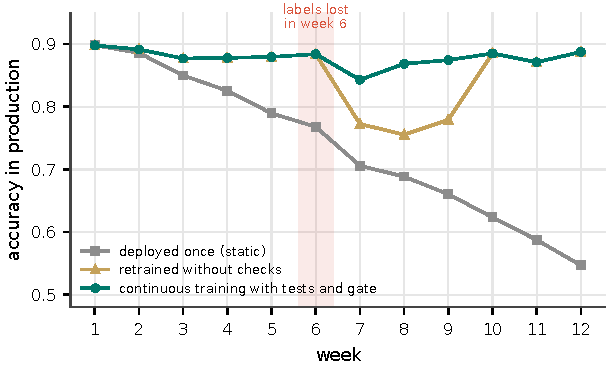
\includegraphics[width=0.78\textwidth]{ch05/continuous_training}
\caption{Accuracy in production of a static model, of weekly retraining without checks, and of continuous
training with a data test and a quality gate, under concept drift and a data incident in week 6.}
\label{fig:ct}
\end{figure}

The gate deserves a closer look. In this run it never rejects a candidate: every week with valid data
is promoted, once with a loss of 0.002 that lies within the tolerance, so the benefit shown comes from the
data test, not from the gate. The gate is a tolerance on a point estimate, not a statistical test of
non-inferiority. A production gate should fix in advance the loss it can accept and compare the two
models on the same examples with a paired measure of uncertainty (\cref{sec:stats}); failing to show that
the new model is better does not show that it is not worse.

Once a new version passes the gate, it can be released gradually \citep{huyen2022designing}: in \emph{shadow
mode}, it receives a copy of the production traffic but its predictions are not used; in a \emph{canary
release}, it serves a small fraction of the users, growing if everything goes well; in an \emph{A/B test},
the old and the new version serve random halves of the users, and the decision is made on business metrics
\citep{kohavi2020trustworthy}. Watching what happens after the release is the subject of Unit~6.

% ---------------------------------------------------------------------
\section{Case study: ModelOps for predictive maintenance}\label{sec:mannco}

\citet{dubovikov2019managing} describes a team that built predictive maintenance models for a manufacturing
company. The models had to be adapted and retrained constantly, and separately for each plant, and several
data scientists worked on them at the same time. The team assembled its infrastructure step by step:
\begin{itemize}
  \item \emph{collaboration and code management}: a GitLab server to share the code, and the GitFlow
        branching model so that everyone followed the same rules for features, releases and fixes;
  \item \emph{project structure}: a PyScaffold template with its data science extension, which gave every
        project the same layout for code, notebooks, data, models and documentation, and integrated well with
        Anaconda environments; repeated code was moved into the project's package, and stable code into its
        source and scripts directories, with a single entry point to train a new model version;
  \item \emph{data versioning}: DVC, with the company's internal file server as remote storage, and DVC
        pipelines to make every experiment reproducible;
  \item \emph{experiment tracking}: an MLflow server with a shared database, so that every team member could
        browse and compare the results of the models for the different plants;
  \item \emph{notebooks in pipelines}: the team liked to prototype in Jupyter notebooks, and used papermill to
        execute them from the command line as steps of the DVC pipelines;
  \item \emph{testing}: a suite of pytest tests, run by GitLab CI/CD on every commit;
  \item \emph{serving and delivery}: the customer wanted a simple API, so the models were served with MLflow,
        packaged with the code in Docker images built by GitLab CI/CD and pushed to a Docker registry.
\end{itemize}
The resulting process had seven steps: make changes to the code; run pre-commit checks of code quality and
style; run the tests in GitLab CI/CD; package the code and the trained models into a Docker image; push the
image to the registry; and, after a manual confirmation in the GitLab interface, run the update command on
the customer's server, which replaces the running container with the new version. Every tool in the list is
simple; what made the difference was combining them into a pipeline that runs without anyone having to
remember the steps.

% ---------------------------------------------------------------------
\section{Building your technology stack}\label{sec:stack}

There is no single right stack: the choice depends on the size of the team and of the project, on the
infrastructure of the organisation and its customers, and on the skills available. \Cref{tab:stack} lists
widely used open-source options for each need. Two principles help: start with the simplest tool that solves
a real problem (a CSV experiment log before a tracking server, a script before an orchestrator), and add
tools only when their benefit outweighs the cost of learning and maintaining them. A small, well-integrated
stack is better than a large collection of tools that nobody fully masters.

\begin{table}[htbp]
\centering\small
\caption{A toolbox for ModelOps.}\label{tab:stack}
\begin{tabularx}{\textwidth}{@{}>{\raggedright\arraybackslash}p{3.4cm}X@{}}
\toprule
Need & Tools\\
\midrule
Code collaboration & GitHub, GitLab, Bitbucket\\
Static code analysis & Flake8 (with extensions such as wemake), MyPy, pre-commit hooks\\
Project templates & PyScaffold (with its data science extension), Cookiecutter\\
Environments & venv/virtualenv, pyenv, pipenv, Poetry, Conda\\
Testing & pytest, Hypothesis\\
CI/CD servers & Jenkins, GitLab CI/CD, GitHub Actions, Travis CI, CircleCI\\
Data versioning & DVC, Git LFS\\
Pipelines & DVC pipelines, MLflow Projects\\
Experiment tracking & MLflow, Sacred, DVC\\
Model exchange & ONNX, PMML\\
Serving & Flask, FastAPI, MLflow models, TensorFlow Serving \citep{olston2017tensorflow}\\
Packaging and deployment & Docker, Kubernetes, Ansible\\
\bottomrule
\end{tabularx}
\end{table}

% ---------------------------------------------------------------------
\section{Summary}\label{sec:summary5}

\begin{itemize}
  \item The deployment option follows from the requirements of latency, hardware, network, privacy, cost and
        complexity. Streaming APIs answer each request when it arrives; batch jobs precompute predictions
        whose features are known in advance, much more efficiently; hybrid systems combine both at the price
        of complexity.
  \item Client-side deployment removes servers and keeps data on the device, but requires small models:
        quantisation, fewer features and distillation can shrink a model by orders of magnitude with little
        loss of accuracy.
  \item Federated learning trains a shared model from data that never leave the devices, and allows
        personalised models; updates must still be protected.
  \item Native serialisation ties production to the training environment and is unsafe with untrusted
        files. PMML is a declarative, auditable standard, popular in regulated industries; ONNX, a widely used open format, also covers deep learning and runs fast on servers, browsers and phones.
        Exported models must be checked against the originals.
  \item ModelOps adapts DevOps to data science, adding data versioning, experiment tracking and tests of data
        and models to version control, CI/CD, packaging and deployment.
  \item Continuous training pipelines retrain and redeploy models automatically; data tests and quality gates
        stop bad data and bad models from reaching production.
  \item Applications built on large language models are deployed as prompts, retrieval and guardrails around a
        model that runs behind an API or on the organisation's hardware. Prompts are code; the retriever can be
        measured with ranking metrics; outputs need tests; and prompt injection needs specific defences.
\end{itemize}

\section*{Bibliographic notes}
\addcontentsline{toc}{section}{Bibliographic notes}

\citet{ameisen2020building} covers the path from idea to deployed product, and \citet{huyen2022designing} the
design of production machine learning systems. \citet{dubovikov2019managing} describes ModelOps in the context
of managing data science teams, and \citet{kreuzberger2023mlops} survey MLOps. \citet{sculley2015hidden} and
\citet{paleyes2022challenges} are essential reading on what goes wrong in production. \citet{kairouz2021advances}
review federated learning, and \citet{humble2010continuous} is the classical reference on continuous delivery.

\section*{Exercises}
\addcontentsline{toc}{section}{Exercises}

\begin{enumerate}[label=\textbf{5.\arabic*},ref=5.\arabic*,leftmargin=*,itemsep=6pt]
  \item\label{exr5:choose} Choose a deployment option for each application and justify it: (a) the price of a
        taxi trip quoted when the user asks for it; (b) a daily ranking of the customers a call centre should
        contact; (c) word suggestions in a phone keyboard; (d) a model that reads medical images inside a
        hospital whose data may not leave the building.
  \item\label{exr5:little} A prediction service receives 200 requests per second. Each request occupies a worker for
        50 ms on average, and each server has four workers. How many requests are in the system on average,
        and what is the smallest number of servers whose idealised capacity exceeds the load?

  \item\label{exr5:batch} A model has a fixed cost of 8 ms per call plus 0.05 ms per example. Compute its
        throughput with batches of 1 and of 1000 examples.
  \item\label{exr5:quant} A neural network has 1.2 million parameters. How much memory do they need in 32-bit
        floating point, in 16-bit floating point and in 8-bit integers?
  \item\label{exr5:latency} Inference takes 120 ms on a phone and 15 ms on a server. The network round trip
        takes 80 ms, and the upload speed is 10 Mbit/s. Where should the model run if each request uploads a
        2 MB image? And if it uploads 20 kB of features?
  \item\label{exr5:fedavg} Three clients with 100, 300 and 600 examples return the values 0.2, 0.5 and 0.9 for a
        parameter. What value does federated averaging assign to it?
  \item\label{exr5:privacy} Why is sending model updates instead of data not enough to guarantee privacy? Name two
        techniques that improve it.
  \item\label{exr5:format} Choose a format to move each model, and justify it: (a) a credit scoring model
        that a regulator must audit and that runs in the bank's Java systems; (b) a gradient boosting model
        that must answer single requests in well under a millisecond; (c) an image classifier for Android
        phones and web browsers; (d) a model shared by two data scientists of the same team, who use the
        same environment.
  \item\label{exr5:pickle} Why should a pickle file from an unknown source never be loaded? Why is a PMML
        file safer?
  \item\label{exr5:dvc} Why is it a bad idea to commit a 2 GB CSV file that changes every day to Git? What does
        DVC store in Git instead?
  \item\label{exr5:tests} Classify as unit, integration or end-to-end test: (a) a function that parses dates
        returns the right value for ten formats; (b) the whole training pipeline runs on 1\% of the data and
        produces a model file; (c) the full pipeline is run on the complete data and the model reaches the
        expected accuracy. Propose an invariance test for a model that predicts house prices.
  \item\label{exr5:gate} A new model reaches an accuracy of 0.842 on 2000 validation examples and the production
        model 0.836 on the same examples. (a) Would a gate that promotes any positive difference promote it?
        (b) Is the improvement statistically supported if the new model is right and the old one wrong on 12
        examples and the opposite never happens? And if those counts are 112 and 100?

  \item\label{exr5:order} Put these steps of a continuous training pipeline in order: train a new model, run the
        unit tests, launch the new version, run data quality tests, package the model, fetch new data, test the
        quality of the model.
  \item\label{exr5:isolation} What does each of a virtual environment, a Conda environment and a Docker container
        isolate?
  \item\label{exr5:rag} A RAG assistant finds the right passage among the first three for 92\% of the questions of
        its test set, yet users complain that many of its answers are wrong. Give three possible causes and how you would
        check each of them.
\end{enumerate}

\section*{Solutions to selected exercises}
\addcontentsline{toc}{section}{Solutions to selected exercises}

\begin{description}[font=\bfseries,leftmargin=0pt,itemsep=5pt]
  \item[\ref{exr5:choose}] (a) Server-side streaming: the location and the available drivers exist only at request
        time. (b) Batch: the features are known in advance and nobody needs the ranking before the morning.
        (c) On device: low latency, offline use and private typing (possibly with federated learning).
        (d) On premises, on the hospital's own servers: the data cannot be sent to an external server.
  \item[\ref{exr5:little}] $L=200\cdot0.05=10$ requests in the system on average (Little's law counts waiting requests
        too). A worker serves about 20 requests per second and a server 80, so $200/80=2.5$: at least three
        servers, with an idealised utilisation of $200/240\approx0.83$. The margin for peaks, failures and tail
        latency is decided with a latency objective and a load test, not with Little's law.

  \item[\ref{exr5:batch}] One example per call: $1/8.05$ ms, about 124 predictions per second. Batches of 1000:
        $1000/(8+50)$ ms, about 17,200 per second.
  \item[\ref{exr5:quant}] 4.8 MB, 2.4 MB and 1.2 MB.
  \item[\ref{exr5:latency}] Uploading 2 MB at 10 Mbit/s takes 1.6 s, so the server needs about 1.7 s and the phone
        wins (120 ms). Uploading 20 kB takes 16 ms, so the server needs $80+16+15=111$ ms, slightly less than the
        phone; privacy, offline use and the cost of the servers may still favour the phone.
  \item[\ref{exr5:fedavg}] $(100\cdot0.2+300\cdot0.5+600\cdot0.9)/1000=0.71$.
  \item[\ref{exr5:privacy}] Updates are computed from the data, and an attacker can reconstruct training examples
        from them. Secure aggregation, so that the server sees only the sum of many updates, and differential
        privacy, which adds calibrated noise.
  \item[\ref{exr5:format}] (a) PMML: declarative, readable and auditable, and scored by Java engines. (b) ONNX with
        ONNX Runtime, which avoids the overhead of the Python pipeline at every call (\cref{lst:onnx}); whether it
        meets the budget must be checked with a representative benchmark on the target hardware. (c) ONNX, run
        by ONNX Runtime on Android and by ONNX Runtime Web in the browser, after checking that both support its
        operators; or a LiteRT model for Android plus a separate export for the browser, each with its runtime.
        (d) joblib or pickle, with pinned versions, or an MLflow model.

  \item[\ref{exr5:pickle}] Unpickling can call arbitrary functions chosen by whoever wrote the file, so it can
        execute any code on the machine. A PMML file only describes the model: an engine that implements the
        standard computes the predictions, and no code from the author of the file is run.
  \item[\ref{exr5:dvc}] Git records snapshots, and every daily version of a 2 GB file adds another large object
        (delta compression helps little with such files), so cloning and every operation slow down. DVC keeps a
        small reference to each version in Git and the data elsewhere, and its \texttt{dvc.lock} records which
        data produced which model.

  \item[\ref{exr5:tests}] (a) Unit, (b) integration, (c) end-to-end. Invariance: the predicted price must not change
        when only the identifier of the listing changes, with every feature of the property, including its
        location, held fixed; the name of the street can encode the location, so changing it is not an
        irrelevant transformation.
  \item[\ref{exr5:gate}] (a) Yes: the difference is 0.006, twelve more correct predictions. (b) The answer depends on
        the paired disagreements, not on the two accuracies. With 12 and 0, the exact McNemar test gives
        $p\approx0.0005$: evidence of a difference. With 112 and 100, $p\approx0.45$: no evidence. The standard error of
        one accuracy (about 0.008) is not that of the difference. And not rejecting equality does not show that
        the models are equivalent: a non-inferiority decision needs a margin fixed in advance.

  \item[\ref{exr5:order}] Run the unit tests; fetch new data; run data quality tests; train a new model; test its
        quality; package the model; launch the new version.
  \item[\ref{exr5:isolation}] A virtual environment isolates the Python packages; a Conda environment also isolates
        the Python version and non-Python libraries; a container isolates the whole user space of the operating
        system, including system libraries and configuration. A container shares the kernel of the host.

  \item[\ref{exr5:rag}] (1) The right passage is often not the first one (in \cref{lst:rag}, only 67\% at rank 1) and the
        prompt includes too few passages: measure recall at the number of passages actually used. (2) The test set does not
        look like real questions: sample real questions from the logs and evaluate on them. (3) The model does not use the
        passages, or contradicts them: measure the groundedness of the answers on a sample, by people or with a validated
        judge. Outdated documents in the index are a fourth candidate.
\end{description}


% =====================================================================
%  Unit 6 -- Monitoring and updating models
%  (this file is assembled from src/ch06/*.tex by build_chapter.py)
% =====================================================================
\chapter{Monitoring and Updating Models}\label{ch:monitoring}

Google Flu Trends estimated how many people had influenza from what they searched for on the web, and when it was
launched it was celebrated for detecting outbreaks earlier than official statistics. In the 2012--2013 season it
predicted more than twice the proportion of doctor visits for influenza-like illness that the US Centers for Disease
Control and Prevention reported \citep{lazer2014parable}: the relation between searches and illness had changed,
partly because of changes in the search engine itself, and the model had not. In 2021 the property company Zillow
closed its home-buying business, which bought houses at prices proposed by its models, after they failed to keep up
with the changes of the market; it wrote down hundreds of millions of dollars and cut about a quarter of its workforce
\citep{zillow2021q3}.

Deployment is not the end of a model's life but the beginning of its most dangerous part. The world
that produced the training data keeps changing: customers change their habits, fraudsters change
their tricks, sensors are replaced, a pandemic changes what people buy. A model that was accurate
when it was validated can degrade silently, without any error message, because it keeps producing
predictions with the same confidence. This unit is about noticing and reacting. It covers what to
monitor in a deployed model; the theory and practice of \emph{dataset shift}, the changes in the data
that make models stale, and how to detect them with and without labels; how to adapt models to
shift, from retraining strategies to the correction of covariate and label shift, domain adaptation
and transfer learning; and how to replace a model safely, with shadow deployments, A/B tests and
multi-armed bandits \citep{ameisen2020building,huyen2022designing}.

\begin{objectives}
After studying this unit you should be able to:
\begin{itemize}
  \item decide what to monitor in a deployed model (service, data, predictions, performance and
        business metrics) and evaluate a model whose actions hide the ground truth;
  \item define and recognise the types of dataset shift (covariate shift, prior or label shift, and
        concept drift) and their temporal patterns;
  \item detect data drift without labels (statistical tests, the population stability index and domain
        classifiers) and concept drift with labels (DDM and Page--Hinkley);
  \item choose a retraining strategy, correct label shift and estimate class proportions, and correct
        covariate shift with importance weights;
  \item explain domain adaptation and transfer learning, and apply simple methods such as CORAL,
        feature augmentation and regularisation towards a source model;
  \item deploy updates safely with shadow mode, canaries and A/B tests, size an experiment, avoid the
        peeking trap, and use multi-armed bandits.
  \item monitor applications built on large language models: costs, quality without labels, drift of the
        questions and changes of the model;
\end{itemize}
\end{objectives}

% =====================================================================
\section{Why monitor models?}\label{sec:whymonitor}

Once a model is deployed, its performance must be monitored like that of any other software system;
but a model can fail in ways that ordinary software cannot. When monitoring a model we must answer three
questions: why we monitor it, how, and what actions the monitoring should drive. There are three main
reasons:
\begin{itemize}
  \item \emph{to keep the model fresh}: most models need to be updated regularly to maintain their
        performance, and monitoring tells us when a model is no longer fresh and must be retrained. If we
        estimate the accuracy of a recommender from the implicit feedback of its users (whether they
        click on the recommendations), we can retrain it as soon as that accuracy drops below a threshold;
        and before redeploying, we must check that the new model is better (\cref{sec:safedeploy});
  \item \emph{to detect abuse}: in fraud detection or abuse prevention, some users actively try to defeat
        the model (\cref{sec:adversarial}), and monitoring is the way to notice attacks and estimate their
        success, for instance by raising an alert when the rate of a kind of event crosses a threshold;
  \item \emph{to catch silent failures}: a broken data pipeline, a feature computed differently in
        production than in training, or a change in an upstream system do not crash the model; it simply
        keeps predicting, worse. The incident of \cref{lst:ct}, a week whose labels were lost, is a typical
        example;
  \item \emph{to comply with the law}: for high-risk systems, the AI Act requires providers to monitor their
        performance after deployment and to report serious incidents (\cref{sec:aiact}).
\end{itemize}

% =====================================================================
\section{Choosing what to monitor}\label{sec:whatmonitor}

A deployed model can be watched at several levels (\cref{fig:monitorlayers}), from the infrastructure
that serves it to the business goal it serves. The lower levels are easier to measure and react faster;
the upper levels are closer to what we care about but are often delayed or hard to observe.

\begin{figure}[htbp]
\centering
\begin{tikzpicture}[font=\scriptsize\sffamily,
  lay/.style={draw=edmnavy,rounded corners=2pt,minimum width=40mm,minimum height=8mm,align=center,font=\scriptsize\sffamily\bfseries},
  note/.style={anchor=west,align=left,text width=88mm}]
  \node[lay,fill=edmcoral!20] (b) at (0,4.0) {business metrics};
  \node[lay,fill=edmgold!30] (p) at (0,3.0) {model performance};
  \node[lay,fill=edmteal!18] (o) at (0,2.0) {predictions (outputs)};
  \node[lay,fill=edmteal!10] (d) at (0,1.0) {input data};
  \node[lay,fill=edmnavy!8] (s) at (0,0.0) {service};
  \node[note] at (2.3,4.0) {click-through rate, conversions, revenue, complaints: the goal of the product};
  \node[note] at (2.3,3.0) {accuracy, calibration, cost, by segment, once the true outcomes arrive
    (often late, sometimes never)};
  \node[note] at (2.3,2.0) {distribution of scores and decisions, rate of each class, confidence};
  \node[note] at (2.3,1.0) {missing values, ranges, distributions and relations of the features (drift)};
  \node[note] at (2.3,0.0) {latency (p50, p99), failed requests, throughput, memory and CPU};
  \draw[-{Stealth[length=2mm]},edmnavy,thick] (-2.6,-0.3) -- (-2.6,4.3)
    node[midway,left,align=right] {closer to\\the goal,\\slower to\\observe};
\end{tikzpicture}
\caption{Levels at which a deployed model can be monitored.}
\label{fig:monitorlayers}
\end{figure}

\paragraph{Service metrics} The average time it takes to process a request, the proportion of requests
that fail, and the resources available (memory, processor) are useful in any production service, and
allow problems to be fixed before many users are affected. For models, the tail of the latency
distribution matters most (\cref{sec:deployoptions}).

\paragraph{Input data and predictions} A model becomes stale when the distribution of its data changes.
Both the inputs and the outputs can change. Changes in the inputs, often called \emph{feature drift} or
\emph{data drift}, are the easiest to track: monitoring can start with summary statistics, such as the mean,
variance and missing rate of the key features, and continue with the methods of \cref{sec:detectshift}.
The distribution of the predictions (the share of each class, the distribution of the scores) is also
easy to track, and a change in it may be a sign that the performance has degraded. But not every change is
a problem: a model that predicts which film a user will watch next should change its predictions when new
films enter the catalogue, even for the same history.

\paragraph{Performance} What we would really like to monitor is the performance of the model, and that
requires the true outcomes, the \emph{ground truth}, which is often hard to obtain. Labels may arrive late
(whether a loan is repaid is known after months) or never. Worse, the actions of the model can prevent us
from observing them: once a transaction is blocked as fraudulent, we never learn whether it really was.
Having access only to a skewed sample of the true distribution makes it impossible to evaluate the model
correctly, and it biases the data for the next model too (a feedback loop, \cref{sec:fairness}).

\emph{Counterfactual evaluation} estimates what would have happened had the model not acted
\citep{bottou2013counterfactual}. The simplest way is to withhold the model's action on a small random
subset of the cases, a \emph{holdout}: the outcomes of those cases are observed whatever the model
predicted, so they form an unbiased sample on which precision and recall can be estimated.
\Cref{lst:holdout} simulates a fraud model that blocks transactions. Among the transactions we can observe,
the fraud rate is 2.6\%, about half of the true 4.6\%, because the model removed many frauds from view. The
2\% holdout estimates the fraud rate (4.3\%), the precision (0.346, against a true 0.361) and the recall
(0.455, against 0.481), with confidence intervals that contain the true values. The price is explicit: 80
frauds that the model would have stopped were let through. In some domains, such as medicine, acting at
random on a subset of patients is not acceptable, and this approach cannot be used.

\begin{pylisting}[label={lst:holdout}]{Estimating precision and recall with a random holdout}
import numpy as np
from sklearn.linear_model import LogisticRegression

rng = np.random.default_rng(0)

def transactions(n):
    X = rng.normal(size=(n, 5))
    logit = -4.5 + 1.5 * X[:, 0] + X[:, 1] - 0.8 * X[:, 2]
    return X, (rng.random(n) < 1 / (1 + np.exp(-logit))).astype(int)   # 1 = fraud

model = LogisticRegression().fit(*transactions(50_000))
X, y = transactions(200_000)                       # one month of production traffic
blocked = model.predict_proba(X)[:, 1] >= 0.2      # the model stops these transactions
holdout = rng.random(len(y)) < 0.02                # 2% of the traffic: never acted upon
observed = ~blocked | holdout                      # transactions whose outcome we see

def precision_recall(pred, truth):
    tp = np.sum(pred & (truth == 1))
    return tp / pred.sum(), tp / truth.sum()

p, r = precision_recall(blocked, y)
print(f"truth (unknowable): fraud rate {y.mean():.4f}, precision {p:.3f}, recall {r:.3f}")
print(f"fraud rate among the transactions we can observe: {y[observed].mean():.4f}")
p_h, r_h = precision_recall(blocked[holdout], y[holdout])
idx = np.flatnonzero(holdout)
boot = [precision_recall(blocked[j], y[j]) for j in
        (rng.choice(idx, len(idx)) for _ in range(1000))]
(pl, rl), (pu, ru) = np.percentile(boot, [2.5, 97.5], axis=0)
print(f"from the holdout: fraud rate {y[holdout].mean():.4f}")
print(f"  precision {p_h:.3f} [{pl:.2f}, {pu:.2f}] recall {r_h:.3f} [{rl:.2f}, {ru:.2f}]")
print(f"price of the holdout: {np.sum(blocked & holdout & (y == 1))} frauds let through")
\end{pylisting}
\begin{pyoutput}
truth (unknowable): fraud rate 0.0462, precision 0.361, recall 0.481
fraud rate among the transactions we can observe: 0.0259
from the holdout: fraud rate 0.0433
  precision 0.346 [0.29, 0.41] recall 0.455 [0.38, 0.53]
price of the holdout: 80 frauds let through
\end{pyoutput}

\paragraph{Business metrics} The most important metrics are those related to the goals of the product. If
every other metric looks good but users do not click on the search results or the recommendations, the
product is failing by definition. Product metrics, such as the \emph{click-through rate} (CTR, the fraction
of displayed recommendations that are clicked), must therefore be monitored closely, and some products are
designed so that their success is easy to track.

\begin{keyidea}
Monitor at every level, and segment the metrics (by country, device, customer type, model version): a
global average can hide a group for which the model has collapsed. Every alert should come with an action
(investigate, roll back, retrain), or it will soon be ignored.
\end{keyidea}

% =====================================================================
\section{Dataset shift}\label{sec:shift}

Almost everything in this book has assumed that the data on which a model is evaluated and used come
from the same distribution as the data on which it was trained. \emph{Dataset shift} is the situation in
which this is not true \citep{quinonero2009dataset,morenotorres2012unifying}. In deployment it is the rule,
not the exception, and the different ways in which the distribution can change have different
consequences and different remedies.

\subsection{Types of shift}

Let $p_s(x,y)$ be the joint distribution of features and target in the training (\emph{source}) data and
$p_t(x,y)$ the distribution in deployment (the \emph{target}). The joint distribution can be factorised in
two ways,
\begin{equation}
  p(x,y)=p(y\mid x)\,p(x)=p(x\mid y)\,p(y),
\end{equation}
and the types of shift are defined by which factors change and which stay the same:
\begin{itemize}
  \item \emph{covariate shift}: the distribution of the features changes, $p_s(x)\neq p_t(x)$, but the
        relationship between features and target does not, $p_s(y\mid x)=p_t(y\mid x)$. A credit model
        trained mostly on young applicants and used for all ages, when the relation between income and
        default is the same at every age, suffers covariate shift;
  \item \emph{prior probability shift}, or \emph{label shift}: the class proportions change,
        $p_s(y)\neq p_t(y)$, but the distribution of the features within each class does not,
        $p_s(x\mid y)=p_t(x\mid y)$. A diagnostic model trained when 5\% of patients had a disease and used
        during an epidemic, when 30\% have it with the same symptoms, suffers label shift;
  \item \emph{concept shift}, or \emph{concept drift}: the relationship itself changes,
        $p_s(y\mid x)\neq p_t(y\mid x)$. Spammers rewrite their messages, so words that indicated spam
        no longer do; a change in the law makes a previously legal transaction fraudulent.
\end{itemize}
These conditions describe useful structures rather than a disjoint taxonomy: label shift generally
changes $p(y\mid x)$ too, through Bayes' rule, while keeping $p(x\mid y)$, so here \emph{concept drift} denotes
changes of the predictive relationship that a change of priors alone does not explain.
In the literature on data streams, a change that affects $p(y\mid x)$, and potentially the optimal
decision boundary, is called \emph{real} drift, and a change that affects only $p(x)$ is called \emph{virtual} drift
\citep{gama2014survey}. Virtual drift is not harmless: a model may be poor in the regions of the input space
that become frequent, and inputs outside the training range are where models extrapolate badly. Other
sources of shift are \emph{sample selection bias} (the training data were not a random sample of the
population, as in \cref{lst:holdout}) and changes in measurement (a new sensor, a new definition of a field),
which create shift where the world has not changed at all.

\Cref{fig:shifttypes} shows the three types on a two-class problem, together with the accuracy of a
logistic regression trained on the original data. Under covariate shift the model remains correct: its
family contains the true boundary, and the accuracy even rises (from 0.85 to 0.88) because the new inputs lie
in an easier region. Under label shift the accuracy hardly changes (0.84), but the model is no longer the
best it could be: its probabilities are miscalibrated, and moving the threshold to account for the new
proportion of positives raises the accuracy to 0.93. Under concept shift the model is useless (0.51).

\begin{figure}[htbp]
\centering
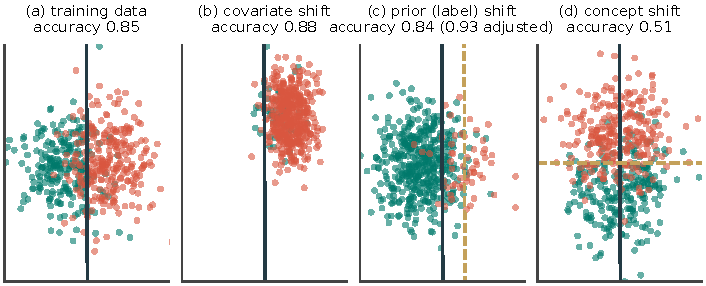
\includegraphics[width=\textwidth]{ch06/shift_types}
\caption{Types of dataset shift on a two-class problem. The solid line is the boundary of a logistic
regression trained on (a); the dashed lines are the boundary adapted to the new prior (c) and the new true
boundary (d). Titles give the accuracy of the original model.}
\label{fig:shifttypes}
\end{figure}

\paragraph{A causal view} Which type of shift is plausible depends on the causal direction of the problem
(\cref{sec:causality}) \citep{schoelkopf2012causal}. When the features cause the target ($X\rightarrow Y$, as
when the characteristics of a loan determine whether it is repaid), the mechanism $p(y\mid x)$ tends to be
stable and the distribution of the causes $p(x)$ is what changes: covariate shift. When the target causes the
features ($Y\rightarrow X$, as when a disease causes symptoms, or a digit causes the image a person writes), the
mechanism $p(x\mid y)$ is the stable part and the prevalence $p(y)$ changes: label shift. This is why label
shift is natural in diagnosis and covariate shift in prediction from causes; but these are hypotheses to
justify, not consequences guaranteed by the direction of the arrows, since stability depends on which
mechanisms actually change.

\paragraph{Patterns over time} Drift also differs in how it unfolds \citep{gama2014survey,webb2016characterizing}
(\cref{fig:driftpatterns}): \emph{sudden} drift replaces a concept by another at once (a new regulation);
\emph{gradual} drift alternates between the old and the new concept, with the new one becoming more frequent
(customers slowly adopting a new product); \emph{incremental} drift moves continuously through intermediate
concepts (a sensor that degrades); and \emph{recurring} drift brings back concepts seen before (seasons,
weekdays and weekends). Recurring concepts suggest keeping old models instead of discarding them.

\begin{figure}[htbp]
\centering
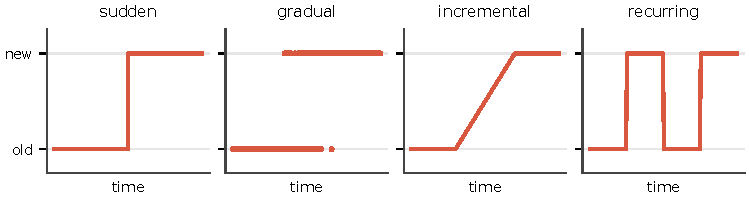
\includegraphics[width=\textwidth]{ch06/drift_patterns}
\caption{Four patterns of concept drift: which concept is active as time goes by.}
\label{fig:driftpatterns}
\end{figure}

% ---------------------------------------------------------------------
\section{Detecting shift}\label{sec:detectshift}

Shift can be detected with or without labels. Without labels we can only see changes in the inputs and in the
predictions, which may or may not affect performance; with labels we can watch the performance itself, but
labels usually arrive late.

\subsection{Without labels: data drift}

\paragraph{Univariate monitoring} The simplest approach compares the distribution of each feature in a
\emph{reference} window (for instance, the training data or the first month in production) with a
\emph{current} window. For numerical features, the two-sample \emph{Kolmogorov--Smirnov} test uses the largest
distance between the two empirical distribution functions, $D=\sup_x|F_{\text{ref}}(x)-F_{\text{cur}}(x)|$; for
categorical features, a $\chi^2$ test compares the frequencies. In credit scoring, the \emph{population
stability index} is a long-standing practice \citep{siddiqi2006credit}: with the proportions $e_i$ of the
reference data and $a_i$ of the current data in each of $B$ bins (usually the deciles of the reference),
\begin{equation}\label{eq:psi}
  \mathrm{PSI}=\sum_{i=1}^{B}\,(a_i-e_i)\,\ln\frac{a_i}{e_i},
\end{equation}
a symmetrised Kullback--Leibler divergence. Conventional thresholds read a PSI below 0.1 as no notable
change, between 0.1 and 0.25 as a moderate one and above 0.25 as a major one; they are conventions of the
index, not significance levels of a test. Its discretisation also has blind spots: a constant feature that
changes to another constant can fall in a single bin and give a PSI of 0, so constant, discrete and
missing values need their own checks.

\paragraph{Multivariate monitoring} Univariate monitors can miss changes in the \emph{relations} between
features. A general alternative is the \emph{domain classifier}, also known as a classifier two-sample test
\citep{lopezpaz2017revisiting}: label the reference examples 0 and the current ones 1, train a classifier, and
measure with cross-validation how well it separates them. An AUC close to 0.5 means that this classifier, with this sample,
cannot tell the two windows apart, which does not prove that their distributions are equal; higher values
indicate a detectable change, though neither a universal measure of distance nor, by themselves, a loss of
predictive performance, and the classifier itself
tells which features changed (through its feature importances, \cref{sec:agnostic}). For a suitable class of
classifiers, its accuracy is also related to the divergence between domains that appears in the bound on the
error of a model trained on one domain and used on the other \citep{bendavid2010theory}; the AUC of a particular
classifier is a diagnostic, not that divergence. Kernel two-sample tests based on the maximum mean discrepancy
\citep{gretton2012kernel}, which we met in \cref{sec:examplebased}, are another option.

\begin{pylisting}[label={lst:datadrift}]{Univariate tests, PSI and a domain classifier on five kinds of change}
import numpy as np
from scipy.stats import ks_2samp
from sklearn.ensemble import HistGradientBoostingClassifier
from sklearn.model_selection import cross_val_score

rng = np.random.default_rng(1)

def window(n=5000, shift=0.0, sd3=1.0, rho=0.8):
    """Three features; x1 and x2 correlated with coefficient rho."""
    cov = np.array([[1, rho, 0], [rho, 1, 0], [0, 0, sd3 ** 2]])
    return rng.multivariate_normal([shift, 0, 0], cov, n)

def psi(ref, cur, bins=10):
    """Population stability index over the deciles of the reference window."""
    edges = np.quantile(ref, np.linspace(0, 1, bins + 1))
    edges[0], edges[-1] = -np.inf, np.inf
    e = np.maximum(np.histogram(ref, edges)[0] / len(ref), 1e-6)
    a = np.maximum(np.histogram(cur, edges)[0] / len(cur), 1e-6)
    return float(np.sum((a - e) * np.log(a / e)))

def domain_auc(ref, cur):
    """Can a classifier tell the two windows apart? An AUC of 0.5 means no."""
    X = np.vstack([ref, cur])
    d = np.r_[np.zeros(len(ref)), np.ones(len(cur))]
    clf = HistGradientBoostingClassifier(max_iter=100, random_state=0)
    return cross_val_score(clf, X, d, cv=5, scoring="roc_auc").mean()

reference = window()
scenarios = {"no drift": window(), "mean of x1 +0.1 sd": window(shift=0.1),
             "mean of x1 +0.5 sd": window(shift=0.5), "sd of x3 x1.5": window(sd3=1.5),
             "correlation 0.8 -> -0.8": window(rho=-0.8)}
print("scenario                  max KS (min p)    max PSI   domain AUC")
for name, current in scenarios.items():
    ks = [ks_2samp(reference[:, j], current[:, j]) for j in range(3)]
    stat, p = max(k.statistic for k in ks), min(k.pvalue for k in ks)
    worst_psi = max(psi(reference[:, j], current[:, j]) for j in range(3))
    print(f"{name:24s}  {stat:.3f} ({p:7.1e})   {worst_psi:.3f}     "
          f"{domain_auc(reference, current):.3f}")
\end{pylisting}
\begin{pyoutput}
scenario                  max KS (min p)    max PSI   domain AUC
no drift                  0.020 (2.5e-01)   0.005     0.493
mean of x1 +0.1 sd        0.051 (4.0e-06)   0.013     0.515
mean of x1 +0.5 sd        0.203 (2.4e-90)   0.241     0.700
sd of x3 x1.5             0.107 (1.6e-25)   0.201     0.604
correlation 0.8 -> -0.8   0.025 (9.7e-02)   0.006     0.892
\end{pyoutput}

\Cref{lst:datadrift} compares the three monitors on windows of 5000 examples with three features, the first two
correlated. Without drift, all of them stay quiet. A shift of the mean of one feature by 0.1 standard deviations
is \emph{statistically significant} for the Kolmogorov--Smirnov test ($p=4\cdot10^{-6}$), but its PSI is 0.013 and
the domain classifier barely notices it (AUC 0.515): with large windows, tests detect changes too small to
matter, so their $p$-values must not be read as measures of importance. A shift of half a standard deviation is
caught by all of them (PSI 0.24, AUC 0.70), and so is a change of the variance of the third feature. But when the
correlation between the first two features changes from 0.8 to $-0.8$, leaving every marginal distribution
intact, the univariate tests see nothing (the smallest $p$-value is 0.097 and the largest PSI 0.006), while the
domain classifier separates the windows with an AUC of 0.892. Whether a model suffers depends on how it uses the
two features and on their relation with the target, which only an evaluation with outcomes can tell.

Some practical advice applies to all these monitors. Monitoring many features with many tests produces false
alarms by chance, so thresholds must account for multiple testing or be set from the variation observed in
periods known to be stable. In high dimensions, it is often more effective to monitor a few summaries: the
predictions of the model, a low-dimensional projection of the inputs, or the output of a domain classifier
\citep{rabanser2019failing}. And under label shift, the distribution of the predicted labels together with the
confusion matrix measured on validation data allows the new class proportions to be estimated without labels
\citep{lipton2018detecting}, a problem we return to in \cref{sec:labelshift}.

\subsection{With labels: concept drift}

When the true outcomes arrive, we can watch the errors of the model directly. Concept drift detectors monitor
the stream of errors and signal when its rate increases significantly
\citep{gama2014survey,lu2019learning}:
\begin{itemize}
  \item the \emph{drift detection method} (DDM, \citealp{gama2004learning}) treats the errors as Bernoulli
        trials. After $i$ examples, the error rate is $p_i$ with standard deviation
        $s_i=\sqrt{p_i(1-p_i)/i}$. The detector remembers the moment at which $p_i+s_i$ was smallest, with
        values $p_{\min}$ and $s_{\min}$, and enters a \emph{warning} level when $p_i+s_i>p_{\min}+2s_{\min}$
        and a \emph{drift} level when $p_i+s_i>p_{\min}+3s_{\min}$. The examples received since the warning
        are the natural training set for a new model;
  \item the \emph{Page--Hinkley test} \citep{page1954continuous}, a sequential test for a change in the mean,
        accumulates the deviation of each observation from the mean available at that moment,
        $m_t=m_{t-1}+x_t-\bar x_t-\delta$, where $\bar x_t$ is the mean of the first $t$ observations and
        $\delta$ the magnitude of change that is tolerated, and signals an increase when $m_t-\min_{j\leq t}m_j$
        exceeds a threshold $\lambda$ (this one-sided version watches increases of the error rate); the moment of the minimum
        estimates when the change began;
  \item ADWIN (adaptive windowing, \citealp{bifet2007learning}) keeps a window of recent examples and drops its
        oldest part whenever two sub-windows have significantly different means, so that the window grows
        while the concept is stable and shrinks when it changes.
\end{itemize}

\begin{pylisting}[label={lst:conceptdrift}]{Detecting concept drift with DDM and Page--Hinkley, from scratch}
import numpy as np
from sklearn.linear_model import LogisticRegression

rng = np.random.default_rng(2)
T = 6000
X = rng.normal(size=(T, 2))
t = np.arange(T)
angle = np.where(t < 2000, 0.0, np.pi / 2) + np.clip((t - 4000) / 1000, 0, 1) * np.pi / 3
y = ((X * np.c_[np.cos(angle), np.sin(angle)]).sum(axis=1) > 0).astype(int)
y = np.where(rng.random(T) < 0.1, 1 - y, y)       # 10% label noise
# the concept changes suddenly at t = 2000 and incrementally between t = 4000 and 5000

class DDM:
    """Drift detection method (Gama et al., 2004) on a stream of 0/1 errors."""
    def __init__(self, warning=2.0, drift=3.0, min_n=100):
        self.warning, self.drift, self.min_n = warning, drift, min_n
        self.reset()

    def reset(self):
        self.n, self.errors, self.best, self.p_min, self.s_min = 0, 0, np.inf, 0, 0
        self.warning_at = None

    def update(self, error, t):
        """Returns None, or the estimated start of the new concept when drift is found."""
        self.n += 1
        self.errors += error
        p = self.errors / self.n
        s = np.sqrt(p * (1 - p) / self.n)
        if self.n < self.min_n:
            return None
        if p + s < self.best:                       # the best moment seen so far
            self.best, self.p_min, self.s_min = p + s, p, s
        if p + s > self.p_min + self.drift * self.s_min:      # strict: errors needed
            return t if self.warning_at is None else self.warning_at
        if p + s > self.p_min + self.warning * self.s_min:
            self.warning_at = t if self.warning_at is None else self.warning_at
        else:
            self.warning_at = None                  # a false warning
        return None

class PageHinkley:
    """Page-Hinkley test for an increase in the mean of a stream."""
    def __init__(self, delta=0.01, threshold=20):
        self.delta, self.threshold = delta, threshold
        self.reset()

    def reset(self):
        self.n, self.mean, self.m, self.m_min, self.t_min = 0, 0.0, 0.0, 0.0, None

    def update(self, x, t):
        """Returns None, or the estimated change point when the test fires."""
        self.n += 1
        self.mean += (x - self.mean) / self.n
        self.m += x - self.mean - self.delta
        if self.t_min is None or self.m < self.m_min:
            self.m_min, self.t_min = self.m, t
        return self.t_min if self.m - self.m_min > self.threshold else None

def run(detector=None, window=None, start=500, refresh=50, cap=2000):
    """Prequential evaluation: predict each example, then learn its label. Every `refresh`
    examples the model is retrained on the last `window` examples or, with a detector,
    on the data since the last detected change (an adaptive window)."""
    model = LogisticRegression().fit(X[:start], y[:start])
    since, errors, alarms = 0, [], []
    for i in range(start, T):
        e = int(model.predict(X[i:i + 1])[0] != y[i])
        errors.append(e)
        refit = (i - start + 1) % refresh == 0
        if detector is not None:
            change = detector.update(e, i)
            if change is not None:
                alarms.append(i)
                detector.reset()
                since, refit = max(change, i - 100), True   # noisy estimate: bound it
        if refit and (window is not None or detector is not None):
            first = i + 1 - window if window else max(since, i + 1 - cap)
            first = min(first, i + 1 - 30)           # at least 30 examples
            if np.unique(y[first:i + 1]).size == 2:    # both classes needed to refit
                model = LogisticRegression().fit(X[first:i + 1], y[first:i + 1])
    return np.array(errors), alarms

results = {"static model": run(), "sliding window": run(window=300),
           "DDM": run(DDM()), "Page-Hinkley": run(PageHinkley())}
print("                  overall   t < 2000   2000-4000   4000-6000   alarms")
for name, (errors, alarms) in results.items():
    part = [1 - errors[a - 500:b - 500].mean() for a, b in [(500, 2000), (2000, 4000),
                                                           (4000, T)]]
    print(f"{name:18s} {1 - errors.mean():.3f}     {part[0]:.3f}      {part[1]:.3f}"
          f"       {part[2]:.3f}    {', '.join(map(str, alarms)) or '-'}")
\end{pylisting}
\begin{pyoutput}
                  overall   t < 2000   2000-4000   4000-6000   alarms
static model       0.533     0.874      0.514       0.295    -
sliding window     0.863     0.865      0.851       0.873    -
DDM                0.862     0.870      0.856       0.863    2046, 4568, 4707
Page-Hinkley       0.863     0.870      0.853       0.867    2040, 4442, 5248
\end{pyoutput}

\Cref{lst:conceptdrift} and \cref{fig:conceptdrift} simulate a stream of 6000 examples whose concept changes
suddenly at $t=2000$ (the boundary rotates by 90 degrees) and incrementally between $t=4000$ and 5000 (it rotates
continuously by another 60 degrees). The evaluation is \emph{prequential}: each example is first predicted and then used for
learning once its label arrives. Four strategies are compared: a static model, which falls to an accuracy of
0.51 after the sudden drift and 0.30 at the end; a sliding window, which retrains every 50 examples on the last
300; and two adaptive windows, which retrain every 50 examples on all the data since the last change detected by
DDM or by Page--Hinkley. Both detectors signal the sudden drift within 40 to 46 examples. In the stable period
the adaptive windows use more data than the sliding window and are slightly better (0.870 against 0.865); after
the sudden drift they recover slightly better too (0.856 and 0.853 against 0.851); during the incremental drift they
signal two changes each but lag behind the sliding window, which forgets continuously (0.863 and 0.867 against
0.873). Overall the three adaptive strategies are tied at 0.86, but only the detectors tell a person that
something changed, and when. An alarm signals a change in \emph{performance}: by itself it does not identify
a change of $p(y\mid x)$, which a covariate shift towards regions where the model is worse, problems with
the labels or changes in the predictor can also cause, and a change of concept that leaves the aggregated
error unchanged goes unnoticed.

\begin{figure}[htbp]
\centering
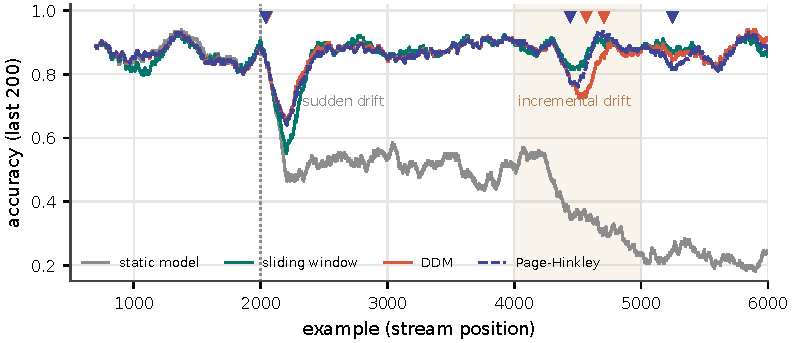
\includegraphics[width=\textwidth]{ch06/concept_drift}
\caption{Prequential accuracy (moving average of 200 examples) of four strategies on a stream with a sudden
drift at $t=2000$ and an incremental drift between $t=4000$ and 5000. Triangles mark the alarms of DDM and
Page--Hinkley.}
\label{fig:conceptdrift}
\end{figure}

\begin{pitfall}
The moment at which a change began is much harder to estimate than the fact that it happened. In a first version
of this experiment, the adaptive windows started at the beginning of the warning period of DDM or at the minimum
of the Page--Hinkley statistic; both were noisy and fell several hundred examples before the real change, so the
new models kept learning from the old concept, and the detectors did worse than a plain sliding window (0.80
against 0.86). Bounding how far back the new training data may start (here, 100 examples before the alarm) fixed
it. Detectors also raise false alarms, especially early on, when the minimum error rate is estimated from few
examples.
\end{pitfall}

% =====================================================================
\section{Adapting to shift}\label{sec:adapt}

Detecting shift is only useful if we can respond to it. The right response depends on the type of shift and on
the data available: labelled data from the new situation, unlabelled data only, or a few labels.

\subsection{Retraining strategies}

The most common response is to retrain the model with recent data. Several strategies are used in practice, often
combined \citep{gama2014survey,lu2019learning}:
\begin{itemize}
  \item \emph{periodic retraining} (every night, every week), simple and predictable, as in the continuous training
        pipeline of \cref{sec:infrastructure}; its period should match the speed at which the data change;
  \item \emph{triggered retraining}, when a monitor or a detector signals a change, which saves computation in
        stable periods and reacts quickly to sudden drift (\cref{lst:conceptdrift});
  \item \emph{windowing}: training only on the most recent data, with a fixed window or an adaptive one such as
        ADWIN; and \emph{weighting}, which keeps all the data but gives older examples less weight, for instance an
        exponentially decaying one;
  \item \emph{ensembles} that add models trained on recent data and remove or downweight those that perform poorly,
        which can also keep the models of recurring concepts (\cref{ch:hybrid});
  \item \emph{online learning}, which updates the model with each new example: stochastic gradient descent for
        linear models and neural networks, or Hoeffding trees for data streams \citep{domingos2000mining}.
\end{itemize}
Retraining requires labels. When they are scarce or delayed, the methods of the next subsections adapt a model using
unlabelled data from the new situation, provided we know which kind of shift has occurred.

\subsection{Correcting label shift and estimating class proportions}\label{sec:labelshift}

Under label shift the class-conditional distributions $p(x\mid y)$ are unchanged, so a probabilistic classifier
trained on the source can be corrected with Bayes' theorem once the new class priors are known: the new posterior is
proportional to the old one multiplied by the ratio of priors,
\begin{equation}\label{eq:priorcorrection}
  p_t(y\mid x)=\frac{\frac{\pi_t(y)}{\pi_s(y)}\,p_s(y\mid x)}{\sum_{y'}\frac{\pi_t(y')}{\pi_s(y')}\,p_s(y'\mid x)},
\end{equation}
where $\pi_s$ and $\pi_t$ are the class proportions in the source and in the target. The difficulty is that the new
proportions are unknown. Estimating them from unlabelled data is a learning task in its own right, called
\emph{quantification} \citep{forman2008quantifying,gonzalez2017review}. The main methods are:
\begin{itemize}
  \item \emph{classify and count} (CC): the proportion of examples that the classifier assigns to each class. It is
        biased, because the errors of the classifier do not cancel when the proportions change;
  \item \emph{adjusted classify and count} (ACC): corrects CC with the true and false positive rates of the
        classifier, estimated on the source by cross-validation: $\hat\pi=(\mathrm{CC}-\FPR)/(\TPR-\FPR)$;
  \item \emph{probabilistic classify and count} (PCC): the average predicted probability, which works when the
        probabilities are calibrated for the target, and its adjusted variants \citep{bella2010quantification};
  \item the \emph{EM algorithm} of \citet{saerens2002adjusting}: start with $\pi_t=\pi_s$, correct the posteriors with
        \cref{eq:priorcorrection}, re-estimate $\pi_t$ as the average corrected posterior, and repeat until convergence.
        It estimates the new priors and corrects the posteriors at the same time.
\end{itemize}
These corrections rest on assumptions: stable class-conditional distributions, an informative and stable
confusion matrix for ACC (it needs $\TPR\neq\FPR$, and a nearly singular matrix in the multiclass case makes it
unstable), and probabilities that represent the source posteriors for PCC and EM. When the counts are not
informative, ACC can even fall outside $[0,1]$ (with $\mathrm{CC}=0.05$, $\TPR=0.8$ and $\FPR=0.1$ it gives $-0.07$),
and such estimates must be reported as infeasible rather than silently clipped.

\begin{pylisting}[label={lst:labelshift}]{Estimating the new class proportions and correcting the posteriors}
import numpy as np
from sklearn.linear_model import LogisticRegression
from sklearn.metrics import brier_score_loss, log_loss
from sklearn.model_selection import cross_val_predict

rng = np.random.default_rng(3)
mu = np.array([1.0, 0.5, 0.0, -0.5, 0.8])          # how the positive class differs

def sample(n, prior):
    """Same class-conditional distributions p(x|y); only p(y) changes."""
    y = (rng.random(n) < prior).astype(int)
    return rng.normal(size=(n, 5)) + np.outer(y, mu), y

X_s, y_s = sample(5000, 0.5)                       # training data: balanced
model = LogisticRegression().fit(X_s, y_s)
X_t, y_t = sample(20000, 0.1)                      # deployment: 10% positives, no labels
p_t = model.predict_proba(X_t)[:, 1]

cc = np.mean(p_t >= 0.5)                           # classify and count
p_cv = cross_val_predict(LogisticRegression(), X_s, y_s, cv=5,
                         method="predict_proba")[:, 1]          # honest TPR and FPR
tpr, fpr = np.mean(p_cv[y_s == 1] >= 0.5), np.mean(p_cv[y_s == 0] >= 0.5)
acc = (cc - fpr) / (tpr - fpr)                     # adjusted classify and count
if not 0 <= acc <= 1:                              # not a valid prevalence: report it
    print(f"ACC = {acc:.3f} lies outside [0, 1]: the counts are not informative")
pcc = p_t.mean()                                   # probabilistic classify and count

def em_prior(p, prior_s, max_iter=1000, tol=1e-8):
    """Saerens et al. (2002): EM estimate of the new prior and of the posteriors."""
    prior = prior_s
    for _ in range(max_iter):                      # until the prior stops changing
        a = prior / prior_s * p
        post = a / (a + (1 - prior) / (1 - prior_s) * (1 - p))
        prior, old = post.mean(), prior
        if abs(prior - old) < tol:
            break
    return prior, post

em, post = em_prior(p_t, y_s.mean())
print(f"true prevalence {y_t.mean():.3f}; estimated: CC {cc:.3f}, ACC {acc:.3f}, "
      f"PCC {pcc:.3f}, EM {em:.3f}")
for name, q in [("unadjusted model", p_t), ("adjusted by EM", post)]:
    print(f"{name:17s} accuracy {np.mean((q >= 0.5) == y_t):.3f}   "
          f"Brier {brier_score_loss(y_t, q):.4f}   log loss {log_loss(y_t, q):.4f}")
\end{pylisting}
\begin{pyoutput}
true prevalence 0.106; estimated: CC 0.284, ACC 0.099, PCC 0.352, EM 0.104
unadjusted model  accuracy 0.771   Brier 0.1560   log loss 0.4761
adjusted by EM    accuracy 0.906   Brier 0.0724   log loss 0.2484
\end{pyoutput}

\Cref{lst:labelshift} trains a logistic regression on balanced data and deploys it where only 10.6\% of the examples
are positive. Classify and count estimates 28.4\% and probabilistic classify and count 35.2\%, both far off, because
the classifier was trained for a world with 50\% positives. The adjusted count (9.9\%) and EM (10.4\%) are close to the
truth. Correcting the posteriors with the prior estimated by EM, without a single label from the new situation, raises
the accuracy from 0.771 to 0.906 and halves the Brier score and the log loss (\cref{sec:scoring}).

\subsection{Correcting covariate shift}

Under covariate shift $p(y\mid x)$ is unchanged, so why should a model trained on the source fail? If the model can
represent the true relationship and has enough data everywhere, it does not, as \cref{fig:shifttypes}b showed. But
models are always approximations, and training spends their capacity on the regions where the \emph{training} data are
dense, which may not be where the deployment data are. The remedy is \emph{importance weighting}
\citep{shimodaira2000improving}: the expected loss on the target can be written as an expectation on the source,
\begin{equation}
  \E_{(x,y)\sim p_t}\bigl[\ell(f(x),y)\bigr]=\E_{(x,y)\sim p_s}\bigl[w(x)\,\ell(f(x),y)\bigr],\qquad
  w(x)=\frac{p_t(x)}{p_s(x)},
\end{equation}
so training on the source examples weighted by $w(x)$ fits the model where it will be used. The densities are unknown,
but their ratio can be estimated directly: by kernel mean matching \citep{huang2007correcting}, by KLIEP
\citep{sugiyama2008direct}, or, most simply, with a domain classifier that separates source from target inputs
\citep{bickel2009discriminative}: if it estimates the probability $q(x)$ that $x$ comes from the target, with $n_s$ source
and $n_t$ target examples,
\begin{equation}
  \hat w(x)=\frac{n_s}{n_t}\cdot\frac{q(x)}{1-q(x)} .
\end{equation}

\begin{pylisting}[label={lst:covshift}]{Importance weighting under covariate shift}
import numpy as np
from scipy.stats import norm
from sklearn.linear_model import LinearRegression, LogisticRegression

rng = np.random.default_rng(4)
f = lambda x: -x + x ** 3                              # the true regression function
x_s = rng.normal(0.5, 0.5, 200)                        # training inputs
y_s = f(x_s) + rng.normal(0, 0.3, 200)
x_t = rng.normal(0.0, 0.3, 1000)                       # deployment inputs
y_t = f(x_t) + rng.normal(0, 0.3, 1000)                # labels: evaluation and reference
col = lambda x: x.reshape(-1, 1)                       # a misspecified linear model

w_true = norm.pdf(x_s, 0, 0.3) / norm.pdf(x_s, 0.5, 0.5)    # p_target(x) / p_source(x)
both = np.r_[x_s, x_t]
is_target = np.r_[np.zeros(200), np.ones(1000)]
domain = LogisticRegression().fit(np.c_[both, both ** 2], is_target)
q = domain.predict_proba(np.c_[x_s, x_s ** 2])[:, 1]   # P(deployment | x)
w_est = 200 / 1000 * q / (1 - q)                       # the same ratio, from a classifier
fit = lambda x, y, w=None: LinearRegression().fit(col(x), y, sample_weight=w)
fits = {"unweighted": fit(x_s, y_s), "weighted (estimated w)": fit(x_s, y_s, w_est),
        "weighted (true w)": fit(x_s, y_s, w_true),
        "deployment fit (resubstitution)": fit(x_t, y_t)}
for name, m in fits.items():
    mse = np.mean((m.predict(col(x_t)) - y_t) ** 2)
    print(f"{name:32s} slope {m.coef_[0]:+.2f}   MSE on deployment data {mse:.3f}")
ess = lambda w: w.sum() ** 2 / (w ** 2).sum()          # effective sample size
print(f"effective sample size: {ess(w_est):.0f} (estimated w), {ess(w_true):.0f} (true w)"
      " of 200")
\end{pylisting}
\begin{pyoutput}
unweighted                       slope +0.46   MSE on deployment data 0.285
weighted (estimated w)           slope -0.57   MSE on deployment data 0.091
weighted (true w)                slope -0.59   MSE on deployment data 0.091
deployment fit (resubstitution)  slope -0.73   MSE on deployment data 0.089
effective sample size: 76 (estimated w), 79 (true w) of 200
\end{pyoutput}

\Cref{lst:covshift} and \cref{fig:covshift} reproduce the classic example of \citet{shimodaira2000improving}: the true
function is a cubic, the model is a straight line, and the training inputs are centred at 0.5 while the deployment inputs
are centred at 0 with a smaller spread. The ordinary least-squares line fits the training region, where the cubic rises
(slope $+0.46$), and has an error of 0.285 on the deployment data. Weighting by the true density ratio, or by the ratio
estimated with a logistic domain classifier, fits the region where the model will be used (slope $-0.57$) and divides the
error by three (0.091), almost the 0.089 of a line fitted to the deployment data themselves and scored on the same data, a
resubstitution reference rather than an estimate of generalisation.

\begin{figure}[htbp]
\centering
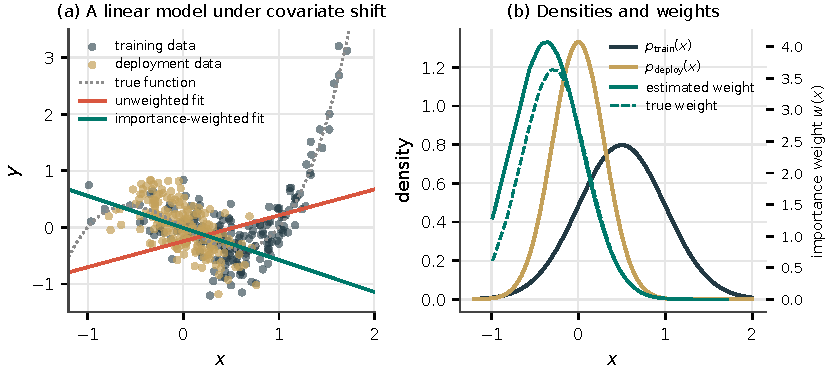
\includegraphics[width=\textwidth]{ch06/covariate_shift}
\caption{Covariate shift. (a) Training and deployment data, the true function, and linear fits without and with
importance weights. (b) The two input densities and the importance weights, true and estimated with a domain
classifier.}
\label{fig:covshift}
\end{figure}

Importance weighting has a price. A few training examples with large weights dominate the fit, which increases the
variance: the \emph{effective sample size}, $(\sum_iw_i)^2/\sum_iw_i^2$, is only 76 of the 200 training examples in the
listing. And the method fails completely where the target has data but the source has none, since no weight can create
information that was never collected: importance weighting needs the support of the target to be covered by the source.
Flattening the weights (raising them to a power between 0 and 1) or clipping them trades bias for variance.

\subsection{Domain adaptation and transfer learning}\label{sec:transfer}

\emph{Domain adaptation} is the general problem of using a model trained in a source domain in a different but related
target domain, with few or no labels in the target; \emph{transfer learning} extends it to related but different tasks
\citep{pan2010survey}. A classic result bounds the error of a model $h$ on the target by its error on the source, plus a
measure of the divergence between the input distributions of the two domains, plus the error of the best model on both
domains together \citep{bendavid2010theory}:
\begin{equation}
  \varepsilon_t(h)\leq\varepsilon_s(h)+\tfrac12\,d_{\mathcal H\Delta\mathcal H}(\mathcal D_s,\mathcal D_t)+\lambda^\star .
\end{equation}
The divergence can be estimated, for a given class of classifiers, with a domain classifier, as in
\cref{lst:datadrift}, and the bound suggests the main families of methods: reduce the divergence by changing
how the data are represented, and keep the source error low. Aligning the inputs is not enough when
$\lambda^\star$ is large: if $p(x)$ is the same in both domains but $y_s=\mathbb 1[x>0]$ and $y_t=\mathbb 1[x<0]$, the
inputs are indistinguishable and the perfect source model is always wrong on the target.
\begin{itemize}
  \item \emph{instance-based} methods reweight or select source examples so that they resemble the target, as
        importance weighting does;
  \item \emph{feature-based} methods map both domains into a representation where they look alike. CORAL
        \citep{sun2016return} aligns the second-order statistics: it whitens the source features with their covariance
        $C_s$ and recolours them with the target covariance $C_t$, $\tilde X_s=(X_s-\mu_s)\,C_s^{-1/2}C_t^{1/2}+\mu_t$, and
        then trains on the transformed source. Domain-adversarial neural networks \citep{ganin2016domain} learn a
        representation that predicts the target well while a domain classifier fails to tell the domains apart;
  \item \emph{parameter-based} methods transfer what a model has learned. With a few target labels, the source model can
        be fine-tuned on them, or a target model can be trained with a penalty that keeps it close to the source model,
        $\min_w\,L_t(w)+\lambda\|w-w_s\|^2$ \citep{chelba2006adaptation}. \emph{Feature augmentation}
        \citep{daume2007frustratingly} triplicates the features into a shared copy and a copy for each domain,
        $\Phi_s(x)=(x,x,0)$ and $\Phi_t(x)=(x,0,x)$, and trains one model on both domains, which learns what is common and
        what is specific to each.
\end{itemize}
Deep learning made transfer the default: the first layers of a network trained on a large data set learn general
features that can be reused for other tasks \citep{yosinski2014transferable}, and today many applications start from a
large pre-trained \emph{foundation model} and adapt it with a few examples or a little fine-tuning
\citep{bommasani2021opportunities}. Transfer can also hurt: when the domains are too different, using the source makes the
target model worse (\emph{negative transfer}), so the transferred model must always be compared with one trained on the
target data alone.

\begin{pylisting}[label={lst:coral}]{Unsupervised domain adaptation with CORAL}
import numpy as np
from scipy.linalg import sqrtm
from sklearn.datasets import make_classification
from sklearn.linear_model import LogisticRegression
from sklearn.model_selection import cross_val_score, train_test_split

X, y = make_classification(n_samples=6000, n_features=10, n_informative=6, random_state=5)
X_s, X_t, y_s, y_t = train_test_split(X, y, test_size=0.5, random_state=0)
rng = np.random.default_rng(5)
gain = np.diag(rng.uniform(0.5, 2.0, 10))                  # recalibrated sensors...
mix = np.eye(10) + 0.3 * rng.normal(size=(10, 10))              # ...with cross-talk
X_t = X_t @ gain @ mix + rng.normal(0, 1, 10)                    # ...and offsets

def coral(X_s, X_t, eps=1.0):
    """CORAL (Sun et al., 2016): give the source the mean and (regularised) covariance of
    the target, approximately."""
    I = np.eye(X_s.shape[1])
    C_s, C_t = np.cov(X_s, rowvar=False) + eps * I, np.cov(X_t, rowvar=False) + eps * I
    recolour = np.real(np.linalg.inv(sqrtm(C_s)) @ sqrtm(C_t))   # whiten, then colour
    return (X_s - X_s.mean(0)) @ recolour + X_t.mean(0)

standardise = lambda Z: (Z - Z.mean(0)) / Z.std(0)
model = lambda: LogisticRegression(max_iter=2000)
print(f"no adaptation             {model().fit(X_s, y_s).score(X_t, y_t):.3f}")
per_domain = model().fit(standardise(X_s), y_s).score(standardise(X_t), y_t)
print(f"standardise each domain   {per_domain:.3f}")
print(f"CORAL                     {model().fit(coral(X_s, X_t), y_s).score(X_t, y_t):.3f}")
print(f"with target labels (CV)   {cross_val_score(model(), X_t, y_t, cv=5).mean():.3f}")
\end{pylisting}
\begin{pyoutput}
no adaptation             0.618
standardise each domain   0.615
CORAL                     0.724
with target labels (CV)   0.841
\end{pyoutput}

\Cref{lst:coral} simulates a common industrial situation: the sensors of a machine are replaced, and the new ones have
different gains and offsets and some cross-talk between channels. A classifier trained on the old sensors has an
accuracy of 0.618 on the new ones. Standardising each domain separately, which corrects the gains and offsets, does not
help (0.615), because the cross-talk mixes the features. CORAL, which needs only unlabelled data from the new sensors,
raises the accuracy to 0.724, well above doing nothing but well below the 0.841 that labelled data from the new sensors
would allow: aligning two moments cannot undo every transformation. With the regularisation of the listing
(a constant added to both covariances), CORAL matches the regularised moments only approximately; and it
uses all the unlabelled target inputs, a legitimate transductive protocol when they are available, whose
moments must be frozen or updated explicitly for new data.

\begin{pylisting}[label={lst:transferlearning}]{Transfer with few target labels: five strategies}
import numpy as np
from scipy.optimize import minimize
from sklearn.linear_model import LogisticRegression

rng = np.random.default_rng(6)
d = 20
w_source = rng.normal(size=d)                       # plenty of labelled data for this one
w_target = w_source + rng.normal(0, 0.5, d)         # a related concept, with few labels

def task(w, n):
    X = rng.normal(size=(n, d))
    return X, (rng.random(n) < 1 / (1 + np.exp(-(X @ w)))).astype(int)

X_s, y_s = task(w_source, 3000)
X_test, y_test = task(w_target, 5000)
LR = lambda: LogisticRegression(fit_intercept=False, max_iter=2000)
w0 = LR().fit(X_s, y_s).coef_[0]
zeros = lambda X: np.zeros_like(X)
augment = lambda X, target: np.c_[X, zeros(X), X] if target else np.c_[X, X, zeros(X)]

def towards_source(X, y, lam=5.0):
    """Logistic regression regularised towards the source weights (parameter transfer)."""
    def loss(w):
        z = X @ w
        return np.mean(np.logaddexp(0, z) - y * z) + lam * np.sum((w - w0) ** 2) / len(y)
    return minimize(loss, w0, method="L-BFGS-B").x

accuracy = lambda w: np.mean(((X_test @ w) > 0) == y_test)
methods = ["target", "source", "pooled", "augmented", "regularised"]
curves = {m: [] for m in methods}
sizes = [10, 20, 50, 100, 200, 500]
for n in sizes:
    scores = {m: [] for m in methods}
    for _ in range(10):
        X_t, y_t = task(w_target, n)
        while y_t.min() == y_t.max():
            X_t, y_t = task(w_target, n)
        scores["target"].append(accuracy(LR().fit(X_t, y_t).coef_[0]))
        scores["source"].append(accuracy(w0))
        pooled = LR().fit(np.r_[X_s, X_t], np.r_[y_s, y_t]).coef_[0]
        scores["pooled"].append(accuracy(pooled))
        aug = LR().fit(np.r_[augment(X_s, False), augment(X_t, True)], np.r_[y_s, y_t])
        scores["augmented"].append(np.mean(aug.predict(augment(X_test, True)) == y_test))
        scores["regularised"].append(accuracy(towards_source(X_t, y_t)))
    for m in methods:
        curves[m].append(np.mean(scores[m]))
print("target labels" + "".join(f"{m:>13s}" for m in methods))
for i, n in enumerate(sizes):
    print(f"{n:13d}" + "".join(f"{curves[m][i]:13.3f}" for m in methods))
\end{pylisting}
\begin{pyoutput}
target labels       target       source       pooled    augmented  regularised
           10        0.649        0.849        0.849        0.819        0.853
           20        0.720        0.849        0.850        0.821        0.854
           50        0.779        0.849        0.850        0.802        0.857
          100        0.831        0.849        0.851        0.836        0.863
          200        0.860        0.849        0.852        0.860        0.870
          500        0.872        0.849        0.855        0.872        0.875
\end{pyoutput}

\Cref{lst:transferlearning} and \cref{fig:transfer} study the case with a few labels. A source task has 3000 labelled
examples; a related target task, whose weights differ from those of the source by random perturbations, has between 10
and 500. Training on the target labels alone needs between 100 and 200 of them to match the source model used as it is (0.849).
Pooling both data sets barely moves away from the source model, because the source examples dominate. Feature augmentation
pays off only with enough target data: with 10 to 50 labels the target-specific copies of the features overfit and the
model is worse than the source model (0.80 to 0.82), and it becomes competitive from 200 labels. Regularising the target
model towards the source weights has the highest mean accuracy at every size in this task and these ten
repetitions, from 0.853 with 10 labels to 0.875 with 500: it starts
from what the source knows and moves only as far as the target data justify.

\begin{figure}[htbp]
\centering
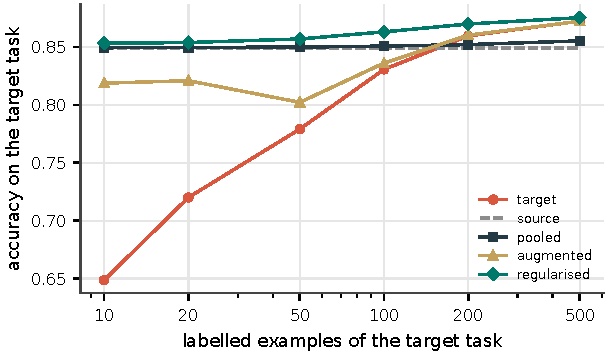
\includegraphics[width=0.75\textwidth]{ch06/transfer}
\caption{Accuracy on a target task as a function of the number of its labelled examples, for a model trained on the
target only, the source model, a model trained on both, feature augmentation, and a target model regularised towards the
source (mean of 10 repetitions).}
\label{fig:transfer}
\end{figure}

% =====================================================================
\section{Monitoring applications built on large language models}\label{sec:llmmonitor}

The applications of \cref{sec:llmapps} need monitoring as much as any other model, and three features make it harder.
Their outputs are free text, which cannot be compared with a label as simply as a class can. Their inputs are open: users
can ask anything, in any language and in any way. And when the model is used through an API, it can change without
notice, because the provider updates it. The levels of \cref{fig:monitorlayers} still apply, with new metrics at each of
them.

\paragraph{Operational metrics} Besides the latency of the whole answer, interactive applications track the \emph{time to
the first token}, which determines how responsive they feel. The number of tokens per request and per user determines the
cost, and must be watched like any other expense: a prompt that grows by accident, or a loop in an agent, can multiply the
bill. Errors, timeouts and rate limits of the provider, and the share of answers served from a cache, complete the picture.

\paragraph{Quality without labels} Most answers are never checked by anybody, so quality is estimated indirectly. Users give
\emph{explicit feedback} (a thumbs up or down) and \emph{implicit feedback}: rephrasing the same question, abandoning the
conversation or asking for a human are signs of a bad answer. A random sample of conversations can be reviewed by people, and
a larger one by a language model acting as a judge, provided that its ratings have first been compared with those of people on
the same sample (\cref{sec:llmapps}). For RAG applications, the share of the claims of each answer that are supported by the
retrieved passages measures its \emph{groundedness}, and the share of questions for which the assistant abstains measures the
gaps in its knowledge: a rising abstention rate means that users are asking about something the index does not cover.

\paragraph{Drift of the questions} What users ask changes: a new product, a news story, a change in the season or an outage
bring new topics, and with them questions the application was not designed or tested for. The methods of \cref{sec:detectshift}
apply directly to text. \Cref{lst:querydrift} represents the questions to a bank's assistant with TF-IDF, as in \cref{lst:rag},
and trains a domain classifier to distinguish the questions of a reference week from those of the current one.

\begin{pylisting}[label={lst:querydrift}]{Detecting drift in the questions asked to an assistant}
import numpy as np
from sklearn.feature_extraction.text import TfidfVectorizer
from sklearn.linear_model import LogisticRegression
from sklearn.model_selection import cross_val_score

rng = np.random.default_rng(19)
TOPICS = {   # what users ask a bank's assistant, by topic
 "balance": ["what is my balance", "how much money do I have", "show my last movements",
             "why is my balance lower than expected"],
 "card": ["my card was blocked", "how do I activate my new card", "card payment declined",
          "I lost my card"],
 "transfer": ["how do I make a transfer", "transfer not received", "cancel a transfer",
              "transfer limit per day"],
 "mortgage": ["mortgage interest rate", "can I repay my mortgage early",
              "documents for a mortgage"],
 "login": ["I cannot log in", "reset my access code", "the app does not open"],
 "bizum": ["how do I send money with bizum", "bizum payment not received",
           "bizum limit per day", "register my phone in bizum"],   # a new service
}
EXTRAS = ["", "please", "hello", "urgent", "thanks", "again", "today"]

def week(n, mix):
    topics, probs = list(mix), np.array(list(mix.values())) / sum(mix.values())
    out = []
    for t in rng.choice(topics, n, p=probs):
        out.append(f"{rng.choice(EXTRAS)} {rng.choice(TOPICS[t])} {rng.choice(EXTRAS)}")
    return out

usual = {"balance": 30, "card": 25, "transfer": 25, "mortgage": 10, "login": 10}
launch = dict(usual, bizum=15)                 # the bank launches instant payments
reference = week(3000, usual)
print("current week compared with the reference   domain AUC   most typical words now")
for name, current in [("same topics", week(3000, usual)),
                      ("new service launched", week(3000, launch))]:
    tfidf = TfidfVectorizer()
    X = tfidf.fit_transform(reference + current)
    d = np.r_[np.zeros(len(reference)), np.ones(len(current))]
    auc = cross_val_score(LogisticRegression(max_iter=1000), X, d, cv=5,
                          scoring="roc_auc").mean()
    coef = LogisticRegression(max_iter=1000).fit(X, d).coef_[0]
    top = tfidf.get_feature_names_out()[np.argsort(-coef)[:3]]
    print(f"{name:40s}   {auc:8.3f}     {', '.join(top) if auc > 0.55 else '-'}")
\end{pylisting}
\begin{pyoutput}
current week compared with the reference   domain AUC   most typical words now
same topics                                   0.507     -
new service launched                          0.573     bizum, with, send
\end{pyoutput}

When the current week has the same mix of topics as the reference, the domain classifier cannot tell them apart (AUC 0.507). When
the bank launches an instant payment service and 15\% of the questions ask about it, the AUC rises to 0.573: a modest value, because
85\% of the questions are as usual, but enough to raise an alert, and the words on which the classifier relies say what changed:
\emph{bizum}, \emph{send} and \emph{with}, from questions such as ``how do I send money with Bizum''. The knowledge base of the
assistant must be extended, and its test set (\cref{sec:llmapps}) with it, before users start receiving invented answers.

\paragraph{Changes in the model} When a provider updates a model behind an API, the behaviour of the application can change from
one day to the next. A study of two widely used models found that their behaviour on several tasks, from solving mathematical
problems to generating code, changed substantially between versions released only three months apart \citep{chen2024chatgpt}. The
defences are those of \cref{sec:safedeploy}: pin the version of the model whenever the provider allows it, run the regression test
set before adopting a new version, and roll it out gradually, in shadow mode or with a canary, comparing the old and new answers on
real traffic.

\paragraph{Safety and security} Applications that talk to the public must also be monitored for abuse: attempts at prompt
injection and at making the model ignore its instructions, leaks of personal data in the answers, and harmful content. Each of
them needs an alert, a person responsible and a procedure to respond. Under the AI Act, chatbots must tell users that they are
talking to a machine, and the providers of high-risk systems must monitor them after deployment and report serious incidents
(\cref{sec:aiact}).

\begin{pitfall}
An assistant that answers fluently is not necessarily answering correctly. Monitoring only the operational metrics of a language
model application (it is fast, cheap and never fails) can hide that its answers have become wrong, because a wrong answer looks
exactly like a right one. Some measure of quality, however indirect, must be part of the dashboard.
\end{pitfall}

% =====================================================================
\section{Deploying updates safely}\label{sec:safedeploy}

Continuous integration and delivery make it easy to release new versions quickly; the challenge is to obtain
evidence, under declared criteria, that they are better. For machine learning, a suite of tests is not enough: a new model can pass every test, beat the
old one on held-out data, and still be worse in production. There is no substitute for live performance, but exposing
users to a worse model has a cost. The usual solution is to move a new model through stages that give progressively
more information at progressively more risk (\cref{fig:rollout}).

\begin{figure}[htbp]
\centering
\begin{tikzpicture}[font=\scriptsize\sffamily,
  st/.style={draw=edmnavy,fill=edmnavy!6,rounded corners=2pt,minimum height=11mm,minimum width=22mm,align=center},
  arr/.style={-{Stealth[length=1.8mm]},edmnavy}]
  \node[st] (a) at (0,0) {offline\\evaluation\\(test data)};
  \node[st] (b) at (2.75,0) {shadow mode\\(predictions\\logged, not used)};
  \node[st] (c) at (5.5,0) {canary\\(a small share\\of users)};
  \node[st] (d) at (8.25,0) {A/B test\\(randomised\\groups)};
  \node[st] (e) at (11.0,0) {full rollout\\(and continued\\monitoring)};
  \foreach \x/\y in {a/b,b/c,c/d,d/e} \draw[arr] (\x) -- (\y);
  \draw[-{Stealth[length=2.2mm]},edmcoral,thick] (-1.1,0.95) -- node[above] {risk for the users} (12.1,0.95);
  \draw[-{Stealth[length=2.2mm]},edmteal,thick] (-1.1,-0.95) -- node[below] {information about the real impact} (12.1,-0.95);
\end{tikzpicture}
\caption{Stages for deploying a new model, from the safest to the most informative.}
\label{fig:rollout}
\end{figure}

\subsection{Why offline evaluation is not enough}

The test data of \cref{ch:evaluation} answer the question ``how good would this model have been on past data?''.
Production asks a different one, and the answers differ for several reasons. The test data are already old when the
model is deployed, and the world may have drifted (\cref{sec:shift}). The features computed in production may differ
from those used in training, because they are computed by different code, from different sources, or with different
delays: this \emph{training--serving skew} is one of the most common causes of failures in production, and it
goes unnoticed by an offline evaluation that uses only the training pipeline, unless the features produced by
the serving path are tested against those of training \citep{breck2019data}. The model's own actions change the data it will see next (a feedback loop).
And users react to a new model in ways that no historical data set can show: a recommender that is more accurate
offline may be less engaging, because it recommends what users would have found anyway.

\subsection{Shadow mode}

In \emph{shadow mode} the new model is deployed in parallel to the existing one: both compute their predictions for
every request and both are logged, but the application uses only those of the existing model. Shadow mode lets
engineers check, on real production traffic and without changing the user experience:
\begin{itemize}
  \item that the infrastructure copes with the new model: latency, memory, failures;
  \item how often the two models agree, and where they disagree (by segment, by input range);
  \item whether the distribution of the new predictions is plausible (the share of each decision, the range of the
        scores);
  \item and, once outcomes arrive, how accurate the new model is on the cases whose representative labels
        are available: if the current policy decides which outcomes are observed (only granted loans are
        repaid or not), the evaluation inherits that selection, and a holdout or a counterfactual design is
        needed.
\end{itemize}
The cost is double computation, and care is needed with side effects: the shadow model must never write to shared
state, send messages or update the features of other models. And one thing shadow mode cannot show is how users
respond to the new model, because they never see its outputs.

\begin{pylisting}[label={lst:shadow}]{Shadow mode catches a training--serving skew}
import numpy as np
from sklearn.ensemble import GradientBoostingClassifier
from sklearn.linear_model import LogisticRegression

rng = np.random.default_rng(10)

def applicants(n):
    income = rng.normal(30, 8, n)                    # thousand EUR
    debt, age = rng.uniform(0, 0.8, n), rng.integers(18, 80, n)
    logit = 0.12 * (income - 30) - 4 * (debt - 0.4) + 0.03 * (age - 45)
    y = (rng.random(n) < 1 / (1 + np.exp(-logit))).astype(int)
    return np.c_[income, debt, age], y

X_train, y_train = applicants(5000)
X_test, y_test = applicants(5000)
# in production
current = LogisticRegression(max_iter=1000).fit(X_train[:, :2], y_train)
candidate = GradientBoostingClassifier(random_state=0).fit(X_train, y_train)
print(f"offline accuracy: current {current.score(X_test[:, :2], y_test):.3f}, "
      f"candidate {candidate.score(X_test, y_test):.3f}")

X_live, y_live = applicants(20000)                   # a week of real requests
served = current.predict(X_live[:, :2])              # what the users receive
X_feed = X_live.copy()
# bug: the new feature service sends EUR
X_feed[:, 0] *= 1000
shadow = candidate.predict(X_feed)                   # computed and logged, never used
print(f"shadow week: agreement {np.mean(served == shadow):.3f}, approval rate "
      f"current {served.mean():.3f}, candidate {shadow.mean():.3f}")
print(f"once the outcomes arrive: current {np.mean(served == y_live):.3f}, "
      f"candidate {np.mean(shadow == y_live):.3f}")
fixed = candidate.predict(X_live)                    # after fixing the units
print(f"after the fix: agreement {np.mean(served == fixed):.3f}, "
      f"candidate accuracy {np.mean(fixed == y_live):.3f}")
\end{pylisting}
\begin{pyoutput}
offline accuracy: current 0.715, candidate 0.727
shadow week: agreement 0.641, approval rate current 0.534, candidate 0.872
once the outcomes arrive: current 0.712, candidate 0.585
after the fix: agreement 0.887, candidate accuracy 0.726
\end{pyoutput}

\Cref{lst:shadow} shows shadow mode catching a typical skew. The candidate, a gradient boosting model with one more
feature, beats the current model offline (0.727 against 0.715). In production, its new feature service sends the income
in euros instead of thousands of euros. During the shadow week the two models agree on only 64\% of the applicants, and
the candidate would approve 87\% of them against 53\% for the current model: a red flag long before any outcome is known.
When the outcomes arrive, the candidate's accuracy is 0.585 (the simulation knows the outcome of every
applicant, which a real bank would not). After the units are fixed, the agreement rises to 89\% and
the candidate's production accuracy (0.726) matches its offline estimate. Had it been deployed directly, every user
would have received the decisions of a broken model.

\subsection{Canary releases and progressive rollout}

A \emph{canary release} serves the new model to a small share of the users (often 1\%) and increases the share in stages,
as long as \emph{guardrail} metrics show no harm: technical ones (error rate, latency) and business ones (conversion,
complaints). If a guardrail is violated, the rollout stops and the previous version is restored automatically. Two practices
make this fast and safe: \emph{blue--green} deployments keep the previous version running, so that switching back is
instantaneous, and \emph{feature flags} turn a model on or off for chosen users without a new deployment. Every deployed
model should be a registered, versioned artefact, so that any earlier version can be redeployed
(\cref{sec:infrastructure}).

\begin{pylisting}[label={lst:canary}]{A progressive rollout with guardrails and automatic rollback}
import numpy as np
from scipy.stats import fisher_exact

rng = np.random.default_rng(11)
STAGES = [0.01, 0.05, 0.20, 0.50, 0.95]   # share of requests for the new model;
DAILY = 100_000                           # 5% stay on the old one as a control
BASE = {"conversion": 0.050, "errors": 0.001}        # the current model

def worse(events_new, n_new, events_old, n_old, higher_is_better, alpha=0.01):
    """Exact one-sided test of harm (Fisher), suitable for rare events such as errors."""
    table = [[events_new, n_new - events_new], [events_old, n_old - events_old]]
    side = "less" if higher_is_better else "greater"
    return fisher_exact(table, alternative=side).pvalue < alpha

def rollout(model):
    exposed = 0
    for share in STAGES:                             # one day of requests per stage
        n_new = int(DAILY * share)
        n_old = DAILY - n_new
        exposed += n_new
        for metric, better in [("errors", False), ("conversion", True)]:   # guardrails
            e_new = rng.binomial(n_new, model[metric])
            e_old = rng.binomial(n_old, BASE[metric])
            if worse(e_new, n_new, e_old, n_old, better):
                return (f"rolled back at {share:.0%} ({metric}), "
                        f"{exposed:,} requests served")
    return f"passed every stage, {exposed:,} requests served during the rollout"

for name, model in [("good model", {"conversion": 0.052, "errors": 0.001}),
                    ("crashes more", {"conversion": 0.050, "errors": 0.020}),
                    ("converts less", {"conversion": 0.046, "errors": 0.001})]:
    print(f"{name:14s} {rollout(model)}")
false = np.mean(["rolled" in rollout(BASE) for _ in range(2000)])
print(f"an identical model is rolled back in {false:.1%} of 2000 rollouts "
      "(10 tests at the 1% level)")
\end{pylisting}
\begin{pyoutput}
good model     passed every stage, 171,000 requests served during the rollout
crashes more   rolled back at 1% (errors), 1,000 requests served
converts less  rolled back at 5% (conversion), 6,000 requests served
an identical model is rolled back in 6.7% of 2000 rollouts (10 tests at the 1% level)
\end{pyoutput}

\Cref{lst:canary} rolls out three candidates through five stages (1\%, 5\%, 20\%, 50\% and 95\% of a day's requests,
keeping 5\% on the old model as a real control until the end), comparing each guardrail with the current model by
an exact one-sided test, suitable for rare events such as errors. A good model goes through. A model that fails 2\%
of its requests is stopped at the first stage, after 1000 requests. In this run, a model whose conversion rate is 4.6\%
instead of 5.0\% is stopped at 5\%, after 6000 requests; but at such small stages a difference like that is detected
only occasionally, and \emph{the absence of an alarm is not evidence that a model is not worse}. The tests have their own
price: with ten tests at the 1\% level, an identical model is rolled back in 6.7\% of the rollouts. A real rollout plan
fixes in advance the acceptable harm, how the budget of false alarms is spread across stages and metrics, and the
evidence required to advance. Canaries catch large problems quickly; to measure small differences reliably we need
a properly designed experiment.

% =====================================================================
\section{A/B testing and experimentation}\label{sec:abtesting}

The principle of an \emph{A/B test}, or online controlled experiment, is simple: expose a random sample of the users to the new
model (the treatment, B) and the rest to the current one (the control, A); after enough time, compare a metric between the groups
and keep the better model \citep{kohavi2009controlled,kohavi2020trustworthy}. Randomisation is what makes the comparison causal
(\cref{sec:causality}): because users are assigned to groups by chance, the groups differ, on average, only in the model they
receive. \Cref{fig:abanatomy} shows the parts of an experimentation system.

\begin{figure}[htbp]
\centering
\begin{tikzpicture}[font=\scriptsize\sffamily,
  st/.style={draw=edmnavy,fill=edmnavy!6,rounded corners=2pt,minimum height=12mm,minimum width=21mm,align=center},
  arr/.style={-{Stealth[length=1.6mm]},edmnavy}]
  \node[st] (u) at (0,0) {request\\from a user};
  \node[st] (h) at (2.45,0) {assignment\\$\mathrm{hash}(\text{salt},\text{id})$\\$\rightarrow$ A or B};
  \node[st] (m) at (4.9,0) {model A\\or model B};
  \node[st] (l) at (7.35,0) {event logs\\(exposures,\\clicks, \dots)};
  \node[st] (k) at (9.8,0) {metrics\\per group};
  \node[st,fill=edmgold!20] (a) at (12.25,0) {analysis: SRM\\check, intervals,\\decision};
  \foreach \x/\y in {u/h,h/m,m/l,l/k,k/a} \draw[arr] (\x) -- (\y);
\end{tikzpicture}
\caption{The anatomy of an online experiment.}
\label{fig:abanatomy}
\end{figure}

\subsection{Designing the experiment}

An experiment starts with a hypothesis (``the new ranking model increases the purchases per user'') and with decisions that must
be taken before it starts:
\begin{itemize}
  \item the \emph{randomisation unit}: usually the user, so that each person has a consistent experience; sessions or requests
        give more units but break consistency, and in marketplaces or social networks, where users influence each other,
        groups of connected users or periods of time may have to be randomised instead;
  \item the \emph{metrics}: one main metric, or overall evaluation criterion, that defines success and that the change is expected
        to move; \emph{guardrail} metrics that must not get worse (latency, errors, revenue, unsubscriptions); and \emph{invariant}
        metrics that the treatment should not affect beyond sampling variation, the first of which is the share of users
        in each group;
  \item the \emph{groups}: users in both groups should be as similar as possible, so that any difference in the outcome can be
        attributed to the model and not to a difference between cohorts (if group A contained all the heavy users and group B only
        occasional ones, the experiment would be inconclusive), which randomisation achieves; the treatment group must be large
        enough to detect the effect, but as small as possible to limit the exposure to a potentially worse model;
  \item the \emph{duration}: long enough to reach the planned sample size, in whole weeks to average out weekly cycles, and long
        enough for \emph{novelty} and \emph{primacy} effects (users reacting to the change itself) to fade; too long, and users may
        be lost. Effects that take months to appear, such as changes in retention, are measured with long-term holdout groups
        \citep{hohnhold2015focusing}.
\end{itemize}

\subsection{Assigning users and checking the assignment}

The simplest infrastructure stores the group of each user with the rest of their information, and lets the system decide which
model serves each request; this works well when users are logged in. Equivalently, and without storage, a user can be assigned by
hashing their identifier together with an experiment-specific \emph{salt}: the same user always gets the same variant, and
different salts make the assignments of different experiments independent, which is what allows large companies to run many
experiments at the same time on the same users \citep{tang2010overlapping}. Independent assignment does not stop the
interventions themselves from interacting when two experiments change the same part of the product, which platforms
handle with layers of mutually exclusive experiments. Experiments assume that each user is exposed to only
one variant, an assumption broken if users see several (for instance on different devices); identifying anonymous users with
cookies or network addresses requires more infrastructure and is less reliable.

The first analysis of any experiment is a sanity check of the assignment. A \emph{sample ratio mismatch} (SRM), a split of users
between the groups significantly different from the intended one, means that something is broken: a variant that crashes for some
users and loses their logs, a redirect that drops users, a bot filter that acts differently on each variant. An SRM alarm calls
for an investigation before the results can be trusted, however good they look \citep{fabijan2019diagnosing}; like any
test it has false alarms, and the absence of an SRM does not certify the rest of the logging.

\begin{pylisting}[label={lst:srm}]{Hash-based assignment and the sample ratio mismatch check}
import hashlib
import numpy as np
from scipy.stats import chisquare

def variant(user, experiment, share_b=0.5):
    """Deterministic assignment: hash the user with an experiment-specific salt."""
    digest = hashlib.sha256(f"{experiment}:{user}".encode()).hexdigest()
    return "B" if int(digest[:8], 16) / 16 ** 8 < share_b else "A"

users = [f"user{i}" for i in range(100_000)]
first = np.array([variant(u, "new-ranker") for u in users])
second = np.array([variant(u, "new-colours") for u in users])
print("same user, same variant every time:", variant("user42", "new-ranker") == first[42])
both_b = np.mean((first == "B") & (second == "B"))
print(f"share in B in both experiments: {both_b:.3f} (independent: 0.250)")

def srm(n_a, n_b, share_b=0.5):
    """Sample ratio mismatch: do the observed counts match the intended split?"""
    total = n_a + n_b
    return chisquare([n_a, n_b], [total * (1 - share_b), total * share_b]).pvalue

alarm = lambda p: "SRM alarm" if p < 0.001 else "no alarm"   # strict: run on every test
n_a, n_b = np.sum(first == "A"), np.sum(first == "B")
p = srm(n_a, n_b)
print(f"logged users A {n_a:,}, B {n_b:,}: p-value {p:.4f}, {alarm(p)}")
lost = int(0.02 * n_b)                    # a bug in B loses 2% of its users' logs
p = srm(n_a, n_b - lost)
print(f"with 2% of B's logs lost: B {n_b - lost:,}, p-value {p:.1e}, {alarm(p)}")
\end{pylisting}
\begin{pyoutput}
same user, same variant every time: True
share in B in both experiments: 0.248 (independent: 0.250)
logged users A 50,423, B 49,577: p-value 0.0075, no alarm
with 2% of B's logs lost: B 48,586, p-value 5.3e-09, SRM alarm
\end{pyoutput}

\Cref{lst:srm} assigns 100,000 users to two experiments by hashing: assignments are consistent, and 24.8\% of the users are in
group B of both experiments, as expected from independent 50/50 splits. The SRM check is a $\chi^2$ test of the observed counts
against the intended split. Because it is run on every experiment, it uses a strict threshold, typically 0.001: the correct
assignment gives $p=0.0075$, no alarm, while losing the logs of 2\% of the users of B gives $p=5\cdot10^{-9}$, a clear alarm.

\subsection{Estimating the better variant}

Most A/B tests compare a metric such as the click-through rate. Deciding which variant is better is more than choosing the group
with the higher rate: the difference must be statistically significant, which for two proportions is usually checked with a
two-sample $z$-test (\cref{sec:stats}),
\begin{equation}
  z=\frac{\hat p_B-\hat p_A}{\sqrt{\hat p\,(1-\hat p)\,\bigl(\frac1{n_A}+\frac1{n_B}\bigr)}},
\end{equation}
where $\hat p$ is the pooled rate. The amount of data needed depends on the rate and on the size of the change to be detected, the
\emph{minimum detectable effect}, and it must be decided \emph{before} the test starts. To detect a change from $p_1$ to $p_2$ with
significance level $\alpha$ and power $1-\beta$, each group needs approximately
\begin{equation}\label{eq:samplesize}
  n=\frac{\Bigl(z_{1-\alpha/2}\sqrt{2\bar p(1-\bar p)}+z_{1-\beta}\sqrt{p_1(1-p_1)+p_2(1-p_2)}\Bigr)^2}{(p_2-p_1)^2},
  \qquad \bar p=\frac{p_1+p_2}{2},
\end{equation}
users. Small effects on small rates need large samples: to detect an increase of the CTR from 5.0\% to 5.5\% with $\alpha=0.05$ and a
power of 0.8, each group needs 31,234 users (\cref{lst:abtest}). The formula assumes one independent opportunity (a click or not) per
user. When users are randomised but each one contributes several impressions, those are not independent, and the
uncertainty of a click-through rate must be computed at the level of users, for instance with a bootstrap over users or
the delta method \citep{deng2018applying}; counting logged events as if they were users overstates the evidence.

\begin{pylisting}[label={lst:abtest}]{Sample size, z-test and the cost of peeking at an A/B test}
import numpy as np
from scipy.stats import norm

def sample_size(p1, p2, alpha=0.05, power=0.8):
    """Users per group to detect a change from p1 to p2 with a two-sided z-test."""
    z_a, z_b = norm.ppf(1 - alpha / 2), norm.ppf(power)
    p = (p1 + p2) / 2
    num = z_a * np.sqrt(2 * p * (1 - p)) + z_b * np.sqrt(p1 * (1 - p1) + p2 * (1 - p2))
    return int(np.ceil(num ** 2 / (p2 - p1) ** 2))

def z_test(clicks_a, n_a, clicks_b, n_b):
    """Two-proportion z-test; works element-wise on arrays."""
    pa, pb = clicks_a / n_a, clicks_b / n_b
    p = (clicks_a + clicks_b) / (n_a + n_b)
    z = (pb - pa) / np.sqrt(p * (1 - p) * (1 / n_a + 1 / n_b))
    return z, 2 * norm.sf(np.abs(z))

n = sample_size(0.050, 0.055)
print(f"users per group to detect a CTR of 5.5% against 5.0%: {n:,}")
rng = np.random.default_rng(7)
a, b = rng.binomial(n, 0.050), rng.binomial(n, 0.055)
z, p = z_test(a, n, b, n)
print(f"one experiment: CTR A {a / n:.4f}, CTR B {b / n:.4f}, z = {z:.2f}, p = {p:.4f}")

looks, reps = 20, 5000                       # A/A tests: no real difference at all
seg = n // looks
users = seg * np.arange(1, looks + 1)
end = peek = 0
for _ in range(reps):
    ca = np.cumsum(rng.binomial(seg, 0.05, looks))
    cb = np.cumsum(rng.binomial(seg, 0.05, looks))
    p = z_test(ca, users, cb, users)[1]
    end += p[-1] < 0.05                       # one test at the planned end
    peek += np.any(p < 0.05)                  # stop as soon as anything looks significant
print(f"false positives in A/A tests: {end / reps:.3f} testing once, "
      f"{peek / reps:.3f} peeking {looks} times")
\end{pylisting}
\begin{pyoutput}
users per group to detect a CTR of 5.5% against 5.0%: 31,234
one experiment: CTR A 0.0498, CTR B 0.0537, z = 2.18, p = 0.0289
false positives in A/A tests: 0.044 testing once, 0.235 peeking 20 times
\end{pyoutput}

The result should be reported as an effect with a confidence interval, not only as a $p$-value: a significant difference may be too
small to matter, and a non-significant one may hide an important effect that the test was too small to detect. When several metrics or
several variants are compared, the chance of a false positive grows with the number of comparisons, and corrections such as Holm's
(\cref{sec:stats}) or a control of the false discovery rate are needed. And results that look too good deserve extra suspicion:
surprising effects in online experiments are more often bugs than discoveries \citep{kohavi2020trustworthy}.

\subsection{Reducing the variance}

The variance of the metric determines how many users an experiment needs. Much of that variance has nothing to do with the treatment:
some users simply use the product more than others. \emph{CUPED} \citep{deng2013improving} removes the part of the variance that can be
predicted from data collected \emph{before} the experiment, such as each user's activity in the previous weeks. With $X$ the pre-experiment
metric and $Y$ the metric during the experiment, it analyses
\begin{equation}
  Y^{\mathrm{cv}}=Y-\theta\,(X-\bar X),\qquad \theta=\frac{\operatorname{cov}(X,Y)}{\operatorname{var}(X)},
\end{equation}
whose mean difference between the groups estimates the same effect, because $X$ was measured before the assignment and cannot be affected by
it, but whose variance is smaller by a factor $1-\rho^2$, where $\rho$ is the correlation between $X$ and $Y$.

\begin{pylisting}[label={lst:cuped}]{Variance reduction with pre-experiment data (CUPED)}
import numpy as np

rng = np.random.default_rng(13)
n = 20_000                                            # users per group
def group(effect):
    # activity score in the month before the test
    before = rng.gamma(2.0, 2.5, n)
    during = 1.0 + 0.8 * before + rng.normal(0, 2.0, n) + effect
    return before, during

xa, ya = group(0.0)
xb, yb = group(0.1)                                   # B adds 0.1 to the activity score
x, y = np.r_[xa, xb], np.r_[ya, yb]
theta = np.cov(x, y)[0, 1] / np.var(x, ddof=1)        # CUPED: Y - theta (X - mean X)
adj = lambda xs, ys: ys - theta * (xs - x.mean())

def summary(a, b):
    diff = b.mean() - a.mean()
    se = np.sqrt(a.var(ddof=1) / n + b.var(ddof=1) / n)
    return diff, 1.96 * se

for name, (a, b) in [("plain difference", (ya, yb)),
                     ("CUPED", (adj(xa, ya), adj(xb, yb)))]:
    diff, half = summary(a, b)
    print(f"{name:17s} effect {diff:+.3f} +/- {half:.3f}   (95% CI)")
rho = np.corrcoef(x, y)[0, 1]
print(f"correlation before/during {rho:.2f}: variance and sample size reduced by "
      f"{rho ** 2:.0%}")
\end{pylisting}
\begin{pyoutput}
plain difference  effect +0.114 +/- 0.068   (95% CI)
CUPED             effect +0.097 +/- 0.039   (95% CI)
correlation before/during 0.82: variance and sample size reduced by 67%
\end{pyoutput}

In \cref{lst:cuped} the correlation between the sessions of each user before and during the experiment is 0.82, so CUPED removes 67\% of
the variance: the 95\% confidence interval of the effect shrinks from $\pm0.068$ to $\pm0.039$ sessions per user, and an experiment would
need a third of the users for the same power.

\subsection{Peeking and sequential tests}

A frequent error is to check the significance continuously and declare the test successful as soon as a significant result appears. Each look
is another chance for noise to cross the threshold, so the real false positive rate is much higher than the nominal one. In
\cref{lst:abtest}, with A/A tests in which both groups receive the same model, testing once at the planned end produces 4.4\% false
positives, close to the nominal 5\%, while looking 20 times and stopping at the first significant result produces 23.5\%; with 100 looks it
reaches 37\% (\cref{fig:experimentation}a).

Looking at the data is not wrong; looking with the wrong threshold is. \emph{Group sequential designs}, developed for clinical trials, plan
a number of looks in advance and use stricter thresholds at each one, so that the overall false positive rate stays at $\alpha$. The
\emph{Pocock} design uses the same threshold at every look \citep{pocock1977group}; the \emph{O'Brien--Fleming} design uses very strict
thresholds at the beginning, which relax towards the end, so that the final test is almost the ordinary one
\citep{obrien1979multiple}; and \emph{alpha spending} functions allow the number and timing of the looks to be flexible
\citep{lan1983discrete}. Methods that give ``always valid'' $p$-values, which can be monitored continuously, are used by commercial
experimentation platforms \citep{johari2017peeking}.

\begin{pylisting}[label={lst:sequential}]{Calibrating group sequential boundaries by simulation}
import numpy as np

rng = np.random.default_rng(14)
K, SIMS = 5, 200_000                                  # five equally spaced looks

def z_paths(drift):
    """z statistics at the K looks; `drift` is the expected z at the final look."""
    steps = rng.normal(drift / np.sqrt(K), 1.0, (SIMS, K))
    return np.cumsum(steps, axis=1) / np.sqrt(np.arange(1, K + 1))

def calibrate(shape, alpha=0.05):
    """Scale a boundary shape so that the overall false positive rate is alpha."""
    null = np.abs(z_paths(0.0))
    lo, hi = 1.0, 6.0
    for _ in range(40):
        c = (lo + hi) / 2
        lo, hi = (c, hi) if np.mean((null > c * shape).any(axis=1)) > alpha else (lo, c)
    return hi * shape

looks = np.arange(1, K + 1)
designs = {"fixed (one test)": np.r_[np.full(K - 1, np.inf), 1.96],
           "Pocock": calibrate(np.ones(K)),
           "O'Brien-Fleming": calibrate(np.sqrt(K / looks))}
null, alt = np.abs(z_paths(0.0)), np.abs(z_paths(1.96 + 0.8416))   # 80% power if fixed
print("design             boundaries at the 5 looks          FPR    power   mean n")
for name, bound in designs.items():
    cross = alt > bound
    stop = np.where(cross.any(axis=1), cross.argmax(axis=1) + 1, K)
    bounds = " ".join(f"{b:5.2f}" if np.isfinite(b) else "    -" for b in bound)
    print(f"{name:17s}  {bounds}   {np.mean((null > bound).any(axis=1)):.3f}  "
          f"{cross.any(axis=1).mean():.3f}   {stop.mean() / K:.0%}")
\end{pylisting}
\begin{pyoutput}
design             boundaries at the 5 looks          FPR    power   mean n
fixed (one test)       -     -     -     -  1.96   0.051  0.799   100%
Pocock              2.41  2.41  2.41  2.41  2.41   0.051  0.711   71%
O'Brien-Fleming     4.55  3.22  2.63  2.28  2.04   0.050  0.789   80%
\end{pyoutput}

\Cref{lst:sequential} calibrates both designs by simulation for five looks. The Pocock threshold is 2.41 at every look; the O'Brien--Fleming
thresholds are 4.55, 3.22, 2.63, 2.28 and 2.04. Both keep the false positive rate at 5\%. With an effect that the single final test would
detect with a power of 0.80, the Pocock design stops earlier on average (it uses 71\% of the maximum sample) but loses power (0.71), while
O'Brien--Fleming keeps almost all of the power (0.79) and still saves 20\% of the users (\cref{fig:sequential}). These boundaries are calibrated for the stated Gaussian
process, five equally spaced looks and a two-sided rule; another schedule of looks or another metric requires
recalibrating them, and the reported rates are Monte Carlo estimates.

\begin{figure}[htbp]
\centering
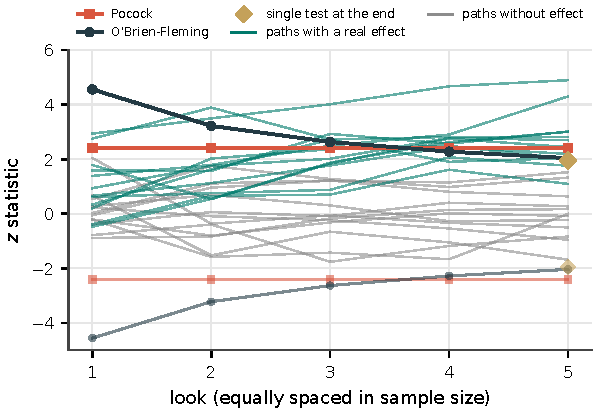
\includegraphics[width=0.72\textwidth]{ch06/sequential}
\caption{Group sequential boundaries for five looks (the test is two-sided: the lower boundaries mirror the upper
ones), with simulated $z$ paths with and without a real effect. A test stops at the first
look at which its path crosses the boundary.}
\label{fig:sequential}
\end{figure}

\subsection{A Bayesian view}

Some teams prefer to report the results of an experiment as probabilities about the variants rather than as $p$-values. With a uniform prior,
the click-through rate of each variant has a Beta posterior, $\mathrm{Beta}(1+\text{clicks},\,1+\text{non-clicks})$, and by drawing from
both posteriors we can estimate the probability that B is better than A, a credible interval for the relative lift, and the \emph{expected
loss} of choosing each variant, the clicks per user we would lose if it were in fact the worse one. A common decision rule is to choose a
variant once its expected loss is below a small threshold.

\begin{pylisting}[label={lst:bayesab}]{Posterior probability, lift and expected loss of an A/B test}
import numpy as np

# the experiment of the z-test listing
rng = np.random.default_rng(7)
n = 31_234
clicks_a, clicks_b = rng.binomial(n, 0.050), rng.binomial(n, 0.055)
draws = np.random.default_rng(15)
# Beta(1 + clicks, 1 + non-clicks): posterior of each CTR with a uniform prior
pa = draws.beta(1 + clicks_a, 1 + n - clicks_a, 200_000)
pb = draws.beta(1 + clicks_b, 1 + n - clicks_b, 200_000)
print(f"clicks A {clicks_a}, B {clicks_b} of {n:,} users each")
print(f"P(CTR of B > CTR of A) = {np.mean(pb > pa):.3f}")
lift = pb / pa - 1
lo, hi = np.percentile(lift, [2.5, 97.5])
print(f"relative lift: {np.median(lift):+.1%}, "
      f"95% credible interval [{lo:+.1%}, {hi:+.1%}]")
for choice, loss in [("A", np.maximum(pb - pa, 0)), ("B", np.maximum(pa - pb, 0))]:
    print(f"expected loss if we choose {choice}: {loss.mean():.5f} clicks per user")
\end{pylisting}
\begin{pyoutput}
clicks A 1557, B 1678 of 31,234 users each
P(CTR of B > CTR of A) = 0.986
relative lift: +7.8%, 95% credible interval [+0.8%, +15.2%]
expected loss if we choose A: 0.00388 clicks per user
expected loss if we choose B: 0.00001 clicks per user
\end{pyoutput}

For the experiment of \cref{lst:abtest} (\cref{lst:bayesab}), the probability that B is better is 0.986, the lift is $+7.8\%$ with a 95\%
credible interval from $+0.8\%$ to $+15.2\%$, and choosing B risks an expected loss of only 0.00001 clicks per user, against 0.00388 for A.
These numbers are easier to communicate than a $p$-value of 0.029, but they rest on the same data. Checking them repeatedly does not invalidate the posterior itself, given an adequate
prior and model, but a decision rule applied at every look does not inherit a given frequentist error rate.

\subsection{Evaluating new models offline from logs}

Every A/B test costs traffic and time, so teams try to discard bad candidates before testing them online. For ranking models,
\emph{interleaving} mixes the results of two rankers in a single list and counts which one's results the user clicks, which detects
differences with far fewer users than an A/B test \citep{chapelle2012large}. More generally, \emph{off-policy evaluation} estimates how a
new decision policy would have performed from the logs of the current one. This requires \emph{support}:
every action that the new policy may choose must have a positive probability under the current policy in that
context, and those probabilities (the \emph{propensities}) must be logged. Randomised logging policies provide it;
deterministic logs can only evaluate the decisions they cover. The \emph{inverse propensity scoring} estimator
\citep{horvitz1952generalization,li2011unbiased} averages, over the logged events, the reward of the events in which the logged action is
the one the new policy would have chosen, divided by the probability with which the current policy chose it:
\begin{equation}
  \hat V(\pi)=\frac1n\sum_{i=1}^{n}\frac{\mathbb 1[a_i=\pi(x_i)]\,r_i}{p(a_i\mid x_i)} .
\end{equation}
For a stochastic new policy, the indicator is replaced by the probability $\pi(a_i\mid x_i)$ that it chooses the logged
action; the estimate refers to the immediate reward, and the policy must be fixed before looking at the logs used to
evaluate it. Doubly robust estimators combine it with a model of the rewards: they remain consistent if either the
propensities or the reward model is correct, and often have lower variance \citep{dudik2011doubly}.

\begin{pylisting}[label={lst:ips}]{Off-policy evaluation of a new recommendation policy}
import numpy as np

rng = np.random.default_rng(16)
# rows: user segment, columns: article
ctr = np.array([[0.05, 0.04, 0.03],
                [0.09, 0.05, 0.04],
                [0.03, 0.04, 0.07]])
segment_share = np.array([0.5, 0.3, 0.2])
logging = np.array([[0.6, 0.2, 0.2],                 # the current, randomised policy
                    [0.6, 0.2, 0.2],
                    [0.2, 0.2, 0.6]])
n = 200_000
s = rng.choice(3, n, p=segment_share)
a = (rng.random(n)[:, None] > np.cumsum(logging[s], axis=1)).sum(axis=1)
r = (rng.random(n) < ctr[s, a]).astype(float)         # the logs: segment, article, click
new = np.array([1, 0, 2])                            # the policy we want to evaluate

truth = np.sum(segment_share * ctr[np.arange(3), new])
match = a == new[s]
naive = r[match].mean()                              # logged events where both agree
terms = match * r / logging[s, a]                    # inverse propensity scoring
ips, se = terms.mean(), terms.std() / np.sqrt(n)
print(f"CTR of the logging policy: {r.mean():.4f}")
print(f"new policy: true CTR {truth:.4f}, naive estimate {naive:.4f}, "
      f"IPS {ips:.4f} +/- {1.96 * se:.4f}")
print(f"the estimates use the {match.sum():,} logged events in which the policies agree")
\end{pylisting}
\begin{pyoutput}
CTR of the logging policy: 0.0552
new policy: true CTR 0.0610, naive estimate 0.0722, IPS 0.0616 +/- 0.0018
the estimates use the 80,167 logged events in which the policies agree
\end{pyoutput}

In \cref{lst:ips}, the current policy shows three articles to three user segments at random, with probabilities that differ by segment. A
new policy would have a click-through rate of 0.0610. Simply averaging the clicks of the logged events in which the old policy happened
to choose what the new one would choose gives 0.0722, an 18\% overestimate, because those events over-represent the segments in which
the agreement was more likely. Weighting by the inverse propensities gives $0.0616\pm0.0018$, an unbiased estimate obtained without showing
the new policy to a single user. Logs of this kind, with their propensities, are also what is needed to evaluate a contextual bandit before deploying it.

% =====================================================================
\section{Multi-armed bandits}\label{sec:bandits}

An A/B test explores for a fixed time and then exploits the winner. \emph{Multi-armed bandits} interleave the two, continuously
\citep{lattimore2020bandit}. The name comes from a gambler facing a row of slot machines (``one-armed bandits'') with unknown payouts. At each
step $t$ we choose an arm $a_t$ (a variant) and receive a reward (a click); each arm $a$ has an unknown expected reward $\mu_a$. The goal is to
maximise the total reward, or equivalently to minimise the \emph{regret}, the expected reward lost by not always choosing the best arm,
\begin{equation}
  R_T=T\mu^\star-\sum_{t=1}^{T}\mu_{a_t},\qquad \mu^\star=\max_a\mu_a .
\end{equation}
The listings compute this \emph{pseudo-regret}, from the expected rewards of the chosen arms rather than the clicks
actually observed, averaged over repetitions.
Every strategy faces the \emph{exploration--exploitation} dilemma: serving the arm that looks best earns now, but trying the others is the
only way to discover whether one of them is better. For stationary bandits with fixed gaps
between the arms, no strategy that performs well on every instance of the problem can have a regret that grows more slowly
than the logarithm of $T$ \citep{lai1985asymptotically} (a strategy that always plays one arm has zero regret where that arm
is the best, and linear regret elsewhere). Good strategies achieve the logarithmic rate, while an A/B test with a fixed
exploration phase, or $\varepsilon$-greedy with a fixed $\varepsilon$, has a regret that grows linearly; explore-then-commit
with an exploration that grows suitably with the horizon can be logarithmic. The main strategies are:
\begin{itemize}
  \item \emph{$\varepsilon$-greedy}: serve the best arm so far, except with probability $\varepsilon$, when a random arm is served. Simple,
        but it explores forever, and as much the clearly bad arms as the promising ones;
  \item \emph{upper confidence bounds} (UCB1, \citealp{auer2002finite}): serve the arm with the highest optimistic estimate, its mean reward
        plus a bonus that shrinks as the arm is tried more, $\bar x_a+\sqrt{2\ln t/n_a}$ (``optimism in the face of uncertainty'');
  \item \emph{Thompson sampling} \citep{thompson1933likelihood,chapelle2011empirical,russo2018tutorial}: keep a posterior distribution for the
        reward of each arm (for click rates, a Beta distribution updated with the clicks and non-clicks), draw a value from each posterior,
        and serve the arm with the highest draw. Arms are served in proportion to the probability that they are the best, so exploration
        concentrates on the arms that might still win \citep{scott2010modern}.
\end{itemize}

\begin{pylisting}[label={lst:bandits}]{An A/B test, epsilon-greedy, Thompson sampling and UCB1 on three variants}
import numpy as np

rng = np.random.default_rng(8)
ctr = np.array([0.050, 0.055, 0.060])              # true click rates, unknown to us
T = 50_000

def ab_test(t, clicks, shows, explore=15_000):     # equal split, then the winner
    return t % 3 if t < explore else int(np.argmax(clicks / shows))

def epsilon_greedy(t, clicks, shows, eps=0.1):     # usually the best so far
    if shows.min() == 0 or rng.random() < eps:
        return int(rng.integers(3))
    return int(np.argmax(clicks / shows))

def thompson(t, clicks, shows):                    # a plausible CTR per variant
    return int(np.argmax(rng.beta(1 + clicks, 1 + shows - clicks)))

# optimism: mean plus an uncertainty bonus
def ucb(t, clicks, shows):
    if shows.min() == 0:
        return int(np.argmin(shows))
    return int(np.argmax(clicks / shows + np.sqrt(2 * np.log(t + 1) / shows)))

def run(policy):
    clicks, shows, regret = np.zeros(3), np.zeros(3), np.empty(T)
    lost = 0.0
    for t in range(T):
        arm = policy(t, clicks, shows)
        clicks[arm] += rng.random() < ctr[arm]
        shows[arm] += 1
        lost += ctr.max() - ctr[arm]               # expected clicks lost by this choice
        regret[t] = lost
    return regret, shows[2] / T

curves = {}
for name, policy in [("A/B test, then winner", ab_test),
                     ("epsilon-greedy", epsilon_greedy), ("Thompson sampling", thompson),
                     ("UCB1", ucb)]:
    runs = [run(policy) for _ in range(10)]
    curves[name] = np.mean([r[0] for r in runs], axis=0)      # mean regret over time
    print(f"{name:22s} clicks lost {np.mean([r[0][-1] for r in runs]):6.1f}   "
          f"traffic to the best variant {np.mean([r[1] for r in runs]):.2f}")
\end{pylisting}
\begin{pyoutput}
A/B test, then winner  clicks lost   97.0   traffic to the best variant 0.71
epsilon-greedy         clicks lost   84.5   traffic to the best variant 0.77
Thompson sampling      clicks lost   47.7   traffic to the best variant 0.85
UCB1                   clicks lost  206.7   traffic to the best variant 0.42
\end{pyoutput}

\Cref{lst:bandits} and \cref{fig:experimentation}b compare four ways of choosing among three variants with click rates of 5.0\%, 5.5\% and 6.0\%,
over 50,000 users. An A/B/C test that splits the first 15,000 users equally and then serves the observed winner loses 97 expected clicks with
respect to always serving the best variant, and sends 71\% of the traffic to it; $\varepsilon$-greedy loses 85 and sends 77\%; Thompson sampling
loses only 48 and sends 85\%. UCB1 is the worst of all (207 clicks lost, 42\% of the traffic to the best variant): its bonus is designed for
rewards anywhere in $[0,1]$, and with click rates around 5\% it dwarfs the differences between the arms, so UCB1 keeps exploring long after the
others have settled. Variants that adapt the bonus to the variance of the rewards fix this, but the lesson is general: the constants of a
bandit algorithm matter as much as its name. These rankings hold for these click rates, settings, horizon and ten
repetitions, not in general.

\begin{figure}[htbp]
\centering
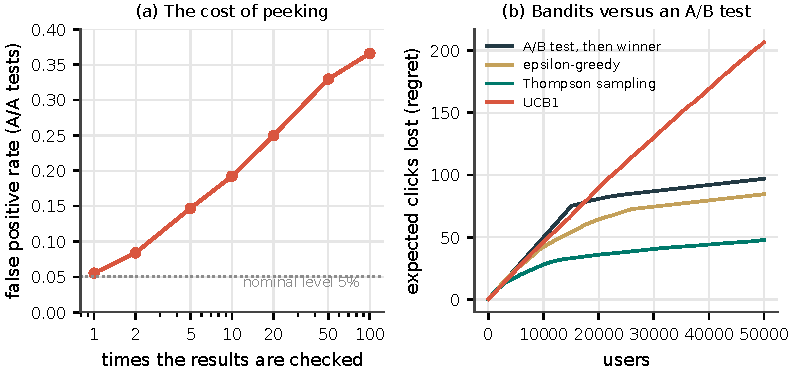
\includegraphics[width=\textwidth]{ch06/experimentation}
\caption{(a) False positive rate of A/A tests when the significance is checked repeatedly and the test stops at the first significant result.
(b) Expected clicks lost by an A/B test followed by the winner, $\varepsilon$-greedy, Thompson sampling and UCB1 (mean of 10 runs).}
\label{fig:experimentation}
\end{figure}

\subsection{When the world changes}

The strategies above assume that the reward of each arm is fixed. When it changes, as everything in this unit does, a bandit that has
accumulated a lot of evidence keeps trusting it: after thousands of plays, its posterior for the old best arm is so concentrated that it takes
a long time to notice that the arm has become the worst. The remedies are the same as for concept drift (\cref{sec:adapt}): forget old evidence,
by discounting it or by using only a sliding window of recent plays \citep{garivier2011upper}, or reset the bandit when a detector signals a
change.

\begin{pylisting}[label={lst:nsbandits}]{Thompson sampling with and without discounting when the best variant changes}
import numpy as np

rng = np.random.default_rng(17)
T, SWITCH = 40_000, 20_000
before = np.array([0.050, 0.055, 0.060])
after = np.array([0.060, 0.055, 0.045])              # the best variant becomes the worst

def run(discount):
    """Thompson sampling; with discount < 1, old evidence fades away."""
    clicks, shows, regret, lost = np.zeros(3), np.zeros(3), np.empty(T), 0.0
    for t in range(T):
        ctr = before if t < SWITCH else after
        arm = int(np.argmax(rng.beta(1 + clicks, 1 + shows - clicks)))
        clicks *= discount
        shows *= discount
        clicks[arm] += rng.random() < ctr[arm]
        shows[arm] += 1
        lost += ctr.max() - ctr[arm]
        regret[t] = lost
    return regret

curves = {}
for name, discount in [("Thompson", 1.0), ("discounted Thompson", 0.999)]:
    curves[name] = np.mean([run(discount) for _ in range(10)], axis=0)
    c = curves[name]
    print(f"{name:20s} clicks lost: {c[SWITCH - 1]:5.1f} before the change, "
          f"{c[-1] - c[SWITCH - 1]:6.1f} after it")
\end{pylisting}
\begin{pyoutput}
Thompson             clicks lost:  50.1 before the change,  161.6 after it
discounted Thompson  clicks lost:  77.5 before the change,   94.3 after it
\end{pyoutput}

In \cref{lst:nsbandits}, the best of three variants becomes the worst halfway through 40,000 users. Standard Thompson sampling loses 50 expected
clicks before the change and 162 after it, while it slowly unlearns the old winner. Discounting the evidence by a factor of 0.999 per play, which
keeps an effective memory of about 1000 plays in total (a half-life of about 700), costs more before the change (78 clicks, because it never becomes completely sure) but recovers much faster
(94 clicks after it), and loses less overall (\cref{fig:banditsadv}a).

\subsection{Contextual bandits}

The best variant is often not the same for every user. \emph{Contextual bandits} choose the variant from the features of the user and the
situation, learning a model of the reward of each arm as a function of the context \citep{li2010contextual}. LinUCB, for instance, fits a ridge
regression of the reward on the context $x$ for each arm, with parameters $\hat\theta_a=A_a^{-1}b_a$ (where $A_a$ accumulates $I+\sum xx^\top$ and
$b_a$ the reward-weighted contexts of the plays of arm $a$), and chooses the arm with the highest optimistic estimate,
\begin{equation}
  a_t=\argmax_a\Bigl(\hat\theta_a^\top x_t+\alpha\sqrt{x_t^\top A_a^{-1}x_t}\Bigr),
\end{equation}
whose bonus is large for contexts unlike those in which the arm has been tried.

\begin{pylisting}[label={lst:linucb}]{A contextual bandit (LinUCB) against a context-free one}
import numpy as np

rng = np.random.default_rng(18)
d, K, T = 5, 3, 20_000
# each variant appeals to different users
theta = rng.normal(0, 1, (K, d))

def ctr(x):
    """Click probability of each variant for a user with features x."""
    return 1 / (1 + np.exp(-(0.6 * theta @ x - 3.0)))

class LinUCB:
    """Li et al. (2010): a ridge regression per variant plus an optimism bonus."""
    def __init__(self, alpha=0.5):
        self.alpha = alpha
        self.A_inv = np.stack([np.eye(d + 1)] * K)
        self.b = np.zeros((K, d + 1))

    def choose(self, x):
        z = np.r_[x, 1.0]
        means = np.einsum("kij,kj,i->k", self.A_inv, self.b, z)
        bonus = np.sqrt(np.einsum("i,kij,j->k", z, self.A_inv, z))
        return int(np.argmax(means + self.alpha * bonus))

    def update(self, arm, x, reward):
        z = np.r_[x, 1.0]
        Az = self.A_inv[arm] @ z                       # Sherman-Morrison update
        self.A_inv[arm] -= np.outer(Az, Az) / (1 + z @ Az)
        self.b[arm] += reward * z

def simulate(policy):
    clicks, shows, lin, lost = np.zeros(K), np.zeros(K), LinUCB(), 0.0
    regret = np.empty(T)
    for t in range(T):
        x = rng.normal(size=d)
        p = ctr(x)
        if policy == "LinUCB":
            arm = lin.choose(x)
        elif policy == "Thompson (no context)":
            arm = int(np.argmax(rng.beta(1 + clicks, 1 + shows - clicks)))
        else:
            arm = int(np.argmax(p))                    # oracle: knows the click rates
        reward = float(rng.random() < p[arm])
        clicks[arm] += reward
        shows[arm] += 1
        lin.update(arm, x, reward)
        lost += p.max() - p[arm]
        regret[t] = lost
    return regret, clicks.sum() / T

results = {}
for policy in ["oracle", "Thompson (no context)", "LinUCB"]:
    regret, rate = simulate(policy)
    results[policy] = regret
    print(f"{policy:22s} CTR {rate:.4f}   expected clicks lost {regret[-1]:7.1f}")
\end{pylisting}
\begin{pyoutput}
oracle                 CTR 0.2019   expected clicks lost     0.0
Thompson (no context)  CTR 0.1289   expected clicks lost  1312.6
LinUCB                 CTR 0.1892   expected clicks lost    92.1
\end{pyoutput}

In \cref{lst:linucb} each of three variants appeals to different users. A context-free Thompson sampler finds the best variant on average and
reaches a click-through rate of 0.129; LinUCB, which uses five features of each user, reaches 0.189
(with a linear model that only approximates the logistic click rates of the simulation, in a single run), close to the 0.202 of an oracle that knows
the best variant for every user, and loses 92 expected clicks against 1313 (\cref{fig:banditsadv}b). Contextual bandits are a form of
personalisation that learns online. The LinUCB of the listing chooses by $\argmax$, deterministically, so its logs do not
support the off-policy evaluation of other policies (\cref{lst:ips}): that requires randomising part of the traffic, for
instance by exploring with a small probability, and logging the actual probability of each chosen action.

\begin{figure}[htbp]
\centering
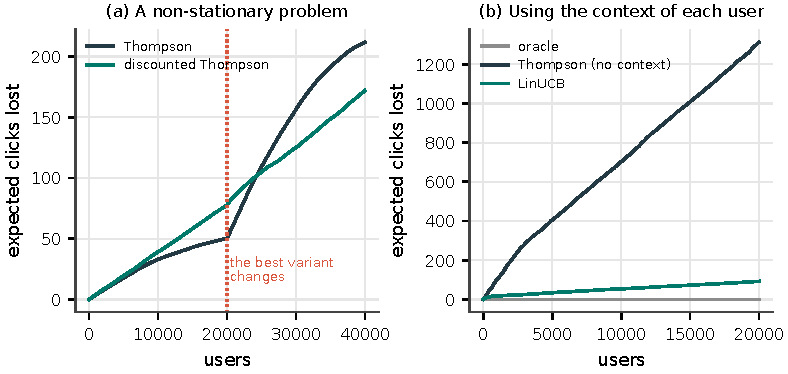
\includegraphics[width=\textwidth]{ch06/bandits_advanced}
\caption{(a) Expected clicks lost by Thompson sampling with and without discounting when the best variant changes. (b) A contextual bandit
(LinUCB) against a context-free one and an oracle (mean of 10 and 1 runs).}
\label{fig:banditsadv}
\end{figure}

\subsection{Bandits in practice}

Real deployments add complications. Rewards arrive with delays (a purchase days after a click), and models are updated in batches rather than
after every request, which reduces the advantage of adaptive allocation. The reward must be chosen carefully: optimising clicks can promote
sensational content at the expense of long-term satisfaction. Because the allocation adapts to the results, the plain averages of the rewards of
each arm are biased, so a bandit is a poor tool for estimating effect sizes. Bandits are the better choice when the goal is to earn while learning,
for short-lived decisions with many alternatives (headlines, creatives, promotions); A/B tests remain preferable when the goal is an unbiased
estimate of the effect of a change on many metrics, including slow ones such as retention. Several companies offer hosted experimentation and
optimisation services for organisations without a dedicated team.

% =====================================================================
\section{Summary}\label{sec:summary6}

\begin{itemize}
  \item Deployed models must be monitored at every level: service, input data, predictions, performance and business metrics.
        When the model's actions hide the ground truth, a random holdout gives unbiased estimates at a known cost.
  \item Dataset shift comes in three main types: covariate shift ($p(x)$ changes, $p(y\mid x)$ does not), label shift ($p(y)$
        changes, $p(x\mid y)$ does not) and concept drift (the predictive relationship changes otherwise); which one is plausible depends on the causal direction of the problem. Drift can be sudden,
        gradual, incremental or recurring.
  \item Without labels, drift is detected in the inputs and predictions: univariate tests and the PSI for each feature, and
        domain classifiers for changes in the joint distribution. Statistical significance is not relevance. With labels,
        detectors such as DDM and Page--Hinkley watch the error rate.
  \item Retraining (periodic, triggered, windowed or online) is the usual response. Label shift can be corrected without labels
        by estimating the new priors (quantification); covariate shift by importance weighting, at the price of variance; domain
        adaptation and transfer learning reuse what a model learned elsewhere.
  \item New models should go through shadow mode, canaries with guardrails and A/B tests. Offline evaluation cannot reveal
        training--serving skew or the reaction of users; shadow mode catches the first, and canaries catch large problems with
        little exposure.
  \item A/B tests need a design fixed in advance (unit, metrics, sample size, duration), a check of the sample ratio, and an analysis
        whose looks follow a valid sequential rule. CUPED reduces the variance with pre-experiment data, sequential designs allow early stopping without
        inflating the errors, and off-policy evaluation estimates new policies from randomised logs.
  \item Multi-armed bandits trade learning and earning continuously. Thompson sampling is a robust default, discounting copes with
        changing rewards, and contextual bandits learn which variant suits each user.
  \item Applications built on language models need monitoring adapted to free text: costs and latency, feedback,
        abstentions and groundedness, the topics of the questions, and the version of the model behind the API.
\end{itemize}

\section*{Bibliographic notes}
\addcontentsline{toc}{section}{Bibliographic notes}

\citet{quinonero2009dataset} and \citet{morenotorres2012unifying} define and classify dataset shift. \citet{gama2014survey} and
\citet{lu2019learning} survey concept drift detection and adaptation, and \citet{rabanser2019failing} compare methods for detecting
shift in practice. \citet{gonzalez2017review} review quantification, \citet{pan2010survey} transfer learning, and
\citet{bendavid2010theory} the theory of domain adaptation. \citet{kohavi2020trustworthy} is the standard guide to online
experiments, with the earlier survey of \citet{kohavi2009controlled}; \citet{deng2013improving} introduced CUPED and
\citet{fabijan2019diagnosing} catalogue the causes of sample ratio mismatches. \citet{lattimore2020bandit} cover bandit algorithms in
depth, and \citet{russo2018tutorial} Thompson sampling. \citet{huyen2022designing} covers monitoring in production machine learning
systems.

\section*{Exercises}
\addcontentsline{toc}{section}{Exercises}

\begin{enumerate}[label=\textbf{6.\arabic*},ref=6.\arabic*,leftmargin=*,itemsep=6pt]
  \item\label{exr6:plan} Propose one metric for each level of \cref{fig:monitorlayers} for a model that recommends products in an
        online shop, and say how quickly each can be observed.
  \item\label{exr6:holdout} A fraud model with a recall of 0.48 processes 200,000 transactions a month, 4.6\% of which are fraudulent.
        How many frauds does a random holdout of 2\% let through each month? And one of 1\%? What do we lose with the smaller holdout?
  \item\label{exr6:psi} A binary feature took the value 1 in 50\% of the reference data and takes it in 60\% of the current data.
        Compute the PSI.
  \item\label{exr6:types} Classify each change as covariate shift, label shift or concept drift: (a) a diagnostic model trained when
        5\% of patients had a disease is used during an epidemic in which 30\% have it, with the same symptoms; (b) a credit model
        trained mostly with young applicants is used for all ages, and the relation between income and default is the same at every
        age; (c) spammers change their vocabulary so that words that indicated spam no longer do; (d) after a software update, a
        sensor reports temperatures in Fahrenheit instead of Celsius.
  \item\label{exr6:saerens} A classifier trained with 50\% positives gives a probability of 0.7 to an example. What is the corrected
        probability if the new proportion of positives is 10\%?
  \item\label{exr6:acc} On new data, a classifier labels 30\% of the examples as positive. Its true and false positive rates, estimated on
        the training data, are 0.80 and 0.10. Estimate the new proportion of positives with adjusted classify and count.
  \item\label{exr6:weights} A domain classifier trained with 200 source and 1000 target examples gives probability 0.6 of coming from the
        target to a source example. What is its importance weight? What is the effective sample size of five examples with weights 1,
        1, 1, 1 and 4?
  \item\label{exr6:ddm} DDM has recorded $p_{\min}=0.10$ and $s_{\min}=0.02$. The current error rate is 0.15 with $s=0.025$. Is it in the
        warning or in the drift level?
  \item\label{exr6:size} How many users per group are needed to detect an increase of the CTR from 10\% to 11\% with $\alpha=0.05$ and a
        power of 0.8?
  \item\label{exr6:peek} Explain why checking an A/B test every day and stopping at the first significant result inflates the false
        positive rate. What can be done instead?
  \item\label{exr6:srm} An experiment meant to split users 50/50 logs 50,600 users in A and 49,400 in B. Is there a sample ratio mismatch?
        What should be done with its results?
  \item\label{exr6:cuped} The correlation between a metric in the weeks before an experiment and during it is 0.6. By how much does CUPED
        reduce the number of users needed in the experiment of \cref{lst:abtest}?
  \item\label{exr6:obf} Why are the O'Brien--Fleming thresholds very high at the first looks and close to 1.96 at the last one? When would you
        prefer them to Pocock's?
  \item\label{exr6:ips} In ten logged events, the new policy agrees with the logged action in three, with rewards 1, 0 and 1 and propensities
        0.5, 0.25 and 0.25. Compute the IPS estimate of the new policy's click rate. Why is it so high?
  \item\label{exr6:bandit} Give one situation where a bandit is preferable to an A/B test, and one where it is not.
  \item\label{exr6:discount} A Thompson sampler discounts its evidence by a factor of 0.999 at every play. Roughly how many plays does it
        remember? What happens if the factor is 0.99?
  \item\label{exr6:shadow} What can shadow mode tell us about a new model, and what can it not?
  \item\label{exr6:negative} How would you detect negative transfer when adapting a model from one hospital to another?
  \item\label{exr6:chatbot} Propose a monitoring dashboard for a customer-service assistant built on a language model,
        with at least one metric for each level of \cref{fig:monitorlayers}. Which metrics would have revealed the launch of
        the service of \cref{lst:querydrift}?
\end{enumerate}

\section*{Solutions to selected exercises}
\addcontentsline{toc}{section}{Solutions to selected exercises}

\begin{description}[font=\bfseries,leftmargin=0pt,itemsep=5pt]
  \item[\ref{exr6:plan}] For example: latency p99 of the recommendation service (seconds); share of requests with missing user history
        and the PSI of the main features (minutes to hours); distribution of the recommended categories (hours); precision of the
        recommendations against later purchases (days); click-through and conversion rates (hours to days).
  \item[\ref{exr6:holdout}] $200{,}000\cdot0.02\cdot0.046\cdot0.48\approx88$ frauds a month; with 1\%, about 44. The smaller holdout halves
        the cost but the estimates become noisier: their confidence intervals widen by a factor of about $\sqrt2$.
  \item[\ref{exr6:psi}] $(0.6-0.5)\ln\frac{0.6}{0.5}+(0.4-0.5)\ln\frac{0.4}{0.5}=0.0182+0.0223=0.041$: below the conventional alert threshold of 0.1.
        This is a heuristic reading of the index, not a test: whether a change of ten points matters depends
        on the application and on the sample sizes.
  \item[\ref{exr6:types}] (a) Label shift. (b) Covariate shift. (c) Concept drift. (d) A change of measurement, or of representation: the same raw number now
        means another temperature, so the relation between the feature and the target changes in the raw
        coordinates and it is not covariate shift. Convert the values back to Celsius and validate the contract
        of the feature before applying the model.
  \item[\ref{exr6:saerens}] $\frac{0.2\cdot0.7}{0.2\cdot0.7+1.8\cdot0.3}=\frac{0.14}{0.68}=0.21$, with the ratios of priors $0.1/0.5=0.2$ and
        $0.9/0.5=1.8$.
  \item[\ref{exr6:acc}] $(0.30-0.10)/(0.80-0.10)=0.29$.
  \item[\ref{exr6:weights}] $\frac{200}{1000}\cdot\frac{0.6}{0.4}=0.3$. Effective sample size $(1+1+1+1+4)^2/(1+1+1+1+16)=64/20=3.2$: five
        examples count as about three.
  \item[\ref{exr6:ddm}] $p+s=0.175$; the warning level is $0.10+2\cdot0.02=0.14$ and the drift level $0.10+3\cdot0.02=0.16$, so drift is
        signalled.
  \item[\ref{exr6:size}] With \cref{eq:samplesize}, $\bar p=0.105$ and $n=(1.96\cdot0.4335+0.8416\cdot0.4335)^2/0.01^2\approx14{,}751$ users per
        group, assuming one independent click opportunity per user and groups of equal size.
  \item[\ref{exr6:peek}] Each look is a new chance for random fluctuations to cross the significance threshold, and stopping at the first
        crossing keeps the false positives and discards the corrections that later data would bring. Fix the sample size in advance
        and test once, or use a sequential design whose thresholds account for the number of looks.
  \item[\ref{exr6:srm}] $\chi^2=600^2/50{,}000+600^2/50{,}000=14.4$, with $p\approx1.5\cdot10^{-4}<0.001$: a mismatch. The results cannot be
        trusted until its cause (a crash, a logging problem, a redirect, a bot filter) is found and fixed.
  \item[\ref{exr6:cuped}] The variance is multiplied by $1-0.6^2=0.64$, so each group needs about $0.64\cdot31{,}234\approx20{,}000$ users instead
        of 31,234.
  \item[\ref{exr6:obf}] Early on there are few data, so only an overwhelming effect should stop the test; most of the error budget is kept for
        the final look, which is almost the ordinary test. Prefer them when the final power matters and early stopping is a bonus for very
        large effects; Pocock's suit situations where stopping early, for instance for harm, is the priority.
  \item[\ref{exr6:ips}] $(1/0.5+0/0.25+1/0.25)/10=(2+0+4)/10=0.6$. With so few events, each rare match is multiplied by a large inverse propensity,
        so the estimate has a huge variance; real off-policy evaluation needs thousands of events and propensities that are not too small. An IPS
        estimate can even exceed 1 in small samples.
  \item[\ref{exr6:bandit}] Preferable: choosing among headlines for a news story that will be read for a few hours. Not preferable: deciding
        whether to launch a new ranking model, where an unbiased estimate of its effect on several metrics, including long-term ones,
        is needed.
  \item[\ref{exr6:discount}] An effective memory of about $1/(1-0.999)=1000$ plays in total (a half-life of about 700). With 0.99 it remembers
        about 100 plays: it forgets ten times faster (how fast it adapts also depends on the click rates and the
        gaps), but with click rates around 5\% its evidence is a handful of clicks, so it keeps exploring and rarely settles on the best variant.
  \item[\ref{exr6:shadow}] It shows the new model's predictions on real production traffic, their agreement with the current model, their
        accuracy on the cases whose outcomes are observed (if the current policy decides which outcomes are
        observed, that evaluation inherits its selection), and whether the infrastructure copes. It cannot show how users react to the new model, because
        they never see its outputs.
  \item[\ref{exr6:negative}] Keep some labelled data from the new hospital as a test set, and compare the adapted model with a model
        trained only on the new hospital's data (and with the original model). If the adapted model is worse than the model trained on
        the new hospital alone, the transfer is hurting.
  \item[\ref{exr6:chatbot}] Service: time to the first token, errors, tokens per request. Inputs: a weekly domain classifier
        on the questions, with its most characteristic words. Outputs: the abstention rate and the length of the answers.
        Quality: the share of negative feedback, of rephrased questions and of requests for a human, and the groundedness of a
        reviewed sample. Business: the share of conversations resolved without a human. The launch would show up in the domain
        classifier, in its words, and in a rising abstention rate.
\end{description}


% =====================================================================
%  Unit 7 -- Applications
%  (this file is assembled from src/ch07/*.tex by build_chapter.py)
% =====================================================================
\chapter{Applications}\label{ch:applications}

In 2015 Netflix\index{Netflix Prize} estimated that about 80\% of the hours streamed on its service were influenced by its
recommendations, and that personalisation and recommendations saved it more than one billion dollars a year, mostly by keeping
subscribers who would otherwise cancel \citep{gomezuribe2015netflix}. This example shows how a model can affect the
results of a company directly, and how evaluation, deployment\index{deployment} and monitoring\index{monitoring} come together in practice.

The previous units built, evaluated, combined, deployed and monitored models in general. This last unit
looks at two families of applications in which machine learning creates direct business value, and at a
tool for putting models in the hands of their users. \emph{Recommender systems\index{recommender system|textbf}} suggest products, films,
songs or people to each user according to their preferences, and they drive a large share of what is
bought, watched and read online. \emph{Customer relationship management\index{customer relationship management (CRM)|textbf}} (CRM) uses data about customers to
decide whom to contact, with what and when; we will see how to design a marketing campaign\index{mailing campaign} with a
probabilistic classifier and cost information, and why the customers most likely to buy are not
necessarily the ones worth contacting. Finally, \emph{Shiny\index{Shiny|textbf}} turns a model into an interactive web
application with a few lines of code. Many ideas from earlier units reappear: ranking metrics and costs
(\cref{ch:evaluation}), causality\index{causality} (\cref{sec:causality}), experiments and bandits\index{multi-armed bandit}
(\cref{sec:abtesting,sec:bandits}) and web applications (\cref{sec:webapps}). The unit closes by following both applications through the whole life cycle, from evaluation to
updating.

\begin{objectives}
After studying this unit you should be able to:
\begin{itemize}
  \item describe the main approaches to recommendation (collaborative filtering\index{collaborative filtering}, content-based\index{content-based filtering} filtering and
        hybrids) and their strengths and weaknesses;
  \item compute user and item similarities and the recommendations of neighbourhood methods by hand, and
        explain matrix factorisation\index{matrix factorisation};
  \item evaluate recommenders for rating prediction and for top-$N$ recommendation, including measures beyond
        accuracy\index{accuracy} such as coverage\index{coverage} and novelty\index{novelty};
  \item design a targeted mailing campaign with a pilot sample, a probabilistic classifier, cumulative response
        curves and profit curves\index{profit curve};
  \item explain uplift\index{uplift modelling} modelling and why it targets different customers than a response model;
\item design a churn model with a temporal protocol, and rank customers by the value that a retention
offer saves;
  \item build an interactive application with Shiny, using reactive\index{reactive programming} expressions to avoid unnecessary computation,
        and test it;
\item plan the evaluation, deployment, monitoring and updating of a recommender or a customer campaign.
\end{itemize}
\end{objectives}

% =====================================================================
\section{Recommender systems}\label{sec:recsys}

Imagine that you want to buy a new phone. You can compare technical features, or you can ask friends and
other people who bought one. Recommender systems\index{recommender system} automate both strategies, and they are widely used: films
and series on streaming platforms, songs and podcasts, products in online shops, hotels and restaurants,
videos, apps, news, jobs and even partners on dating applications. Their input is usually a set of
interactions between users and items, either \emph{explicit} (ratings, likes) or \emph{implicit} (purchases,
clicks, viewing time), which can be arranged as a large and very sparse \emph{user--item matrix}: most users
have interacted with a tiny fraction of the items. The main approaches (\cref{fig:rectaxonomy}) are
\citep{aggarwal2016recommender,ricci2022recommender}:
\begin{itemize}
  \item \emph{collaborative filtering\index{collaborative filtering|textbf}}, which learns from the user--item interactions alone, using
        similarities between users or between items, or models of their latent preferences;
  \item \emph{content-based\index{content-based filtering|textbf} filtering}, which recommends items similar, in their attributes or descriptions, to
        those the user liked;
  \item \emph{hybrid} systems, which combine both, as most large-scale recommenders do.
\end{itemize}

\begin{figure}[htbp]
\centering
\begin{tikzpicture}[font=\scriptsize\sffamily,
  root/.style={draw=edmnavy,fill=edmnavy!12,rounded corners=2pt,minimum height=7mm,align=center,font=\scriptsize\sffamily\bfseries},
  mid/.style={draw=edmnavy,fill=edmnavy!5,rounded corners=2pt,minimum height=7mm,minimum width=27mm,align=center},
  leaf/.style={draw=edmnavy!60,rounded corners=2pt,minimum height=6mm,minimum width=22mm,align=center,font=\tiny\sffamily},
  arr/.style={-{Stealth[length=1.5mm]},edmnavy!80}]
  \node[root] (r) at (0,0) {recommender systems};
  \node[mid] (cf) at (-4.2,-1.2) {collaborative filtering\\(interactions only)};
  \node[mid] (cb) at (0,-1.2) {content-based\\(item descriptions)};
  \node[mid] (hy) at (4.2,-1.2) {hybrid\\(both)};
  \node[leaf] (mb) at (-5.6,-2.5) {memory-based:\\user- or item-based\\neighbours};
  \node[leaf] (mo) at (-2.8,-2.5) {model-based:\\matrix factorisation,\\neural models};
  \node[leaf] (c1) at (0,-2.5) {attributes, text\\(TF-IDF), images};
  \node[leaf] (h1) at (4.2,-2.5) {weighted, switching,\\feature combination};
  \foreach \a/\b in {r/cf,r/cb,r/hy,cf/mb,cf/mo,cb/c1,hy/h1} \draw[arr] (\a) -- (\b);
\end{tikzpicture}
\caption{The main families of recommender systems.}
\label{fig:rectaxonomy}
\end{figure}

% ---------------------------------------------------------------------
\section{Collaborative filtering}\label{sec:cf}

Collaborative filtering\index{collaborative filtering} rests on a simple intuition: users who agreed in the past tend to agree in the future,
so the opinions of users with tastes similar to mine are good predictors of what I will like
\citep{resnick1994grouplens}. Two things must be defined: a measure of the similarity\index{similarity measure} between users, and a way
of combining the opinions of similar users into recommendations, weighted by their similarity
\citep{segaran2007programming}.

\subsection{Similarity between users}

Each user is a row of the rating matrix, a vector with many missing values, and two users can be compared on the
items that both have rated. \Cref{lst:ratingstoy} defines a small, made-up matrix of seven users and six films, and
two classic measures:
\begin{itemize}
  \item a similarity\index{similarity measure} derived from the \emph{Euclidean\index{Euclidean distance|textbf} distance} between the two vectors of common ratings,
        $\mathrm{sim}(u,v)=1/(1+d(u,v))$, which is 1 for identical ratings and decreases with the distance. Users
        become points in a space with one axis per item (\cref{fig:similarity}b). Because it adds up the
        differences, it also falls with the number of common items (a difference of one star gives 0.5 on one
        film and 0.24 on ten), so users with different overlaps are not directly comparable;
  \item the \emph{Pearson\index{Pearson correlation|textbf} correlation} of the common ratings, which measures their linear association after
        centring the ratings of each user, regardless of how generous each one is: a user who always gives one star more than another
        has a correlation of 1 with them (\cref{fig:similarity}a). Other choices are the cosine\index{cosine similarity} of the rating
        vectors, rank correlations (Spearman\index{Spearman correlation}, Kendall) and, for binary interactions, the Jaccard index.
\end{itemize}

\begin{pylisting}[label={lst:ratingstoy}]{A small rating matrix and two similarity measures (file \texttt{ratings\_toy.py})}
"""A small, made-up rating matrix (1-5 stars) and two similarity measures (Unit 7)."""
import numpy as np

nan = np.nan
FILMS = ["Space Saga", "Paris Love", "Heist Night", "Silent Forest", "Laugh Club",
         "Deep Ocean"]
USERS = ["Ana", "Ben", "Carla", "David", "Elena", "Fran", "Ivo"]
R = np.array([[4.5, 2.0, 4.0, 3.0, 2.5, 4.0],      # Ana
              [5.0, 1.5, 4.5, nan, 2.0, 3.5],      # Ben
              [2.0, 4.5, 2.5, 4.0, 4.5, nan],      # Carla
              [nan, 4.0, 2.0, 3.5, 5.0, 2.5],      # David
              [3.5, 3.0, nan, 4.5, 3.0, 4.0],      # Elena
              [4.0, nan, 3.5, 2.0, nan, 4.5],      # Fran
              [4.0, nan, nan, nan, 2.0, 4.5]])     # Ivo, who wants recommendations

def euclidean_similarity(a, b):
    """1 / (1 + Euclidean distance) over the items rated by both."""
    both = ~np.isnan(a) & ~np.isnan(b)
    return 1 / (1 + np.sqrt(np.sum((a[both] - b[both]) ** 2))) if both.any() else 0.0

def pearson(a, b):
    """Pearson correlation over the items rated by both (0 if undefined)."""
    both = ~np.isnan(a) & ~np.isnan(b)
    if both.sum() < 2 or a[both].std() == 0 or b[both].std() == 0:
        return 0.0
    return float(np.corrcoef(a[both], b[both])[0, 1])
\end{pylisting}

\begin{figure}[htbp]
\centering
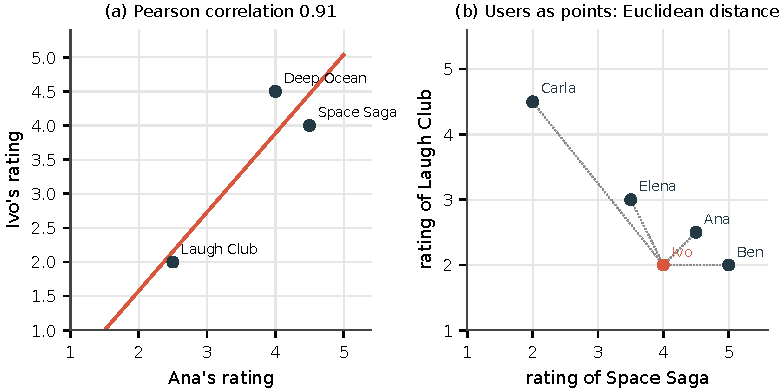
\includegraphics[width=\textwidth]{ch07/similarity}
\caption{(a) Ana's and Ivo's ratings of the three films they have both seen, and the regression line behind their
Pearson correlation. (b) Users as points in the plane of two of the films; the dotted lines are the Euclidean
distances to Ivo in this plane only, not over all the films each pair has in common.}
\label{fig:similarity}
\end{figure}

\subsection{From similar users to recommendations}

To recommend films to Ivo, we could take the most similar user and suggest the film they rated highest among those Ivo
has not seen. This is too local a strategy: it relies on the opinion of a single person and ignores every film that
person has not rated. It is better to combine the ratings of several users, using their similarities as weights. For
an item $i$ that user $u$ has not rated, the predicted rating is the weighted average of the ratings of the users $v$ who
rated it,
\begin{equation}\label{eq:usercf}
  \hat r_{ui}=\frac{\sum_{v}\mathrm{sim}(u,v)\,r_{vi}}{\sum_{v}\mathrm{sim}(u,v)},
\end{equation}
where the sums run over the users with a positive similarity\index{similarity measure} who rated $i$ (often only the $k$ most similar ones).
Dividing by the sum of the similarities of the users who rated \emph{that} item matters: otherwise films seen by many
people would get high totals just for being popular. A refinement predicts deviations from each user's mean rating,
$\hat r_{ui}=\bar r_u+\sum_v\mathrm{sim}(u,v)(r_{vi}-\bar r_v)/\sum_v|\mathrm{sim}(u,v)|$, which corrects for users who
rate generously or harshly.

\begin{pylisting}[label={lst:usercf}]{User-based collaborative filtering with Pearson similarities}
import numpy as np
from ratings_toy import FILMS, R, USERS, euclidean_similarity, pearson

me = USERS.index("Ivo")
print("similarity of Ivo to   " + "  ".join(f"{u:>6s}" for u in USERS[:-1]))
for name, sim in [("Euclidean-based", euclidean_similarity), ("Pearson", pearson)]:
    print(f"{name:22s}" + "  ".join(f"{sim(R[me], R[v]):6.2f}" for v in range(me)))

def recommend(user, sim=pearson):
    """Weighted average of the others' ratings, with positive similarities as weights."""
    rows = []
    for i, film in enumerate(FILMS):
        if not np.isnan(R[user, i]):
            continue                                   # already seen
        total = sim_sum = 0.0
        for v in range(len(USERS)):
            s = sim(R[user], R[v]) if v != user else 0.0
            if s > 0 and not np.isnan(R[v, i]):
                total += s * R[v, i]
                sim_sum += s
        rows.append((film, total, sim_sum, total / sim_sum if sim_sum else np.nan))
    return sorted(rows, key=lambda r: -r[3])

print("film            total   sim. sum   predicted rating")
for film, total, sim_sum, score in recommend(me):
    print(f"{film:14s} {total:6.2f}   {sim_sum:6.2f}       {score:.2f}")
\end{pylisting}
\begin{pyoutput}
similarity of Ivo to      Ana     Ben   Carla   David   Elena    Fran
Euclidean-based         0.54    0.41    0.24    0.22    0.45    1.00
Pearson                 0.91    0.76   -1.00   -1.00    0.94    1.00
film            total   sim. sum   predicted rating
Heist Night     10.53     2.66       3.95
Silent Forest    8.98     2.85       3.15
Paris Love       5.78     2.61       2.22
\end{pyoutput}

\Cref{lst:usercf} computes both similarities between Ivo and the other users and builds the table of
\cref{eq:usercf}: for each unseen film, the total of the similarity-weighted ratings, the sum of the similarities of the
users who rated it, and their ratio. \emph{Heist Night} is the clear recommendation (3.95), and \emph{Paris Love}, loved
by the users whose tastes are opposite to Ivo's, is the clear non-recommendation (2.22). The table also shows a weakness of
the Pearson\index{Pearson correlation} correlation: with only two films in common, it is always $+1$ or $-1$ when both users rated the two films differently
(Carla, David and Fran), whatever the ratings, because two points always lie on a line; it is undefined,
and taken as 0 by the code, when a user gave both films the same rating. In practice, similarities computed on few common items are shrunk towards
zero (\emph{significance weighting}), or a minimum number of common items is required.

\subsection{Item-based collaborative filtering}\label{sec:itemcf}

User-based\index{collaborative filtering!user-based} filtering does not scale well: with millions of users, finding the neighbours of each user at request time is
expensive, and when the catalogue is large two users rarely have enough items in common to be compared reliably. Item-based filtering compares \emph{items}: two films are similar if the users who rated both rated them
alike, which is the same computation applied to the columns of the matrix. To recommend items to a user, we
look for items similar to those the user rated, weighted by their similarity\index{similarity measure} and by the user's ratings
\citep{sarwar2001item}. Similarities between items are more stable than similarities between users, because each item has
many ratings and its audience changes slowly, so the item--item matrix can be precomputed offline and updated
infrequently, which makes recommendation fast. This is how Amazon's recommendations worked at scale
\citep{linden2003amazon}.

A note on terminology: item-based\index{collaborative filtering!item-based} filtering, which some texts call ``content-based\index{content-based filtering}'' because it relies on similarities
between items, is still \emph{collaborative}: the similarities come from the users' ratings. They do not use the attributes of the items. Content-based filtering in the strict sense, which uses the descriptions of the items, is the subject of
\cref{sec:contentbased}.

\begin{pylisting}[label={lst:itemcf}]{Item-based collaborative filtering, and recommending users to an item}
import numpy as np
from ratings_toy import FILMS, R, USERS, pearson

# Item-based: precompute item-item similarities once (the columns of the matrix)
n = len(FILMS)
S = np.array([[pearson(R[:, i], R[:, j]) if i != j else -np.inf for j in range(n)]
              for i in range(n)])
print("films most similar to 'Space Saga':",
      ", ".join(f"{FILMS[j]} ({S[0, j]:+.2f})" for j in np.argsort(-S[0])[:2]))

def recommend_items(user):
    seen = ~np.isnan(R[user])
    scores = {}
    for i in np.flatnonzero(~seen):
        w = np.maximum(S[i, seen], 0)                  # similar items the user has rated
        if w.sum() > 0:
            scores[FILMS[i]] = float(w @ R[user, seen] / w.sum())
    return sorted(scores.items(), key=lambda kv: -kv[1])

print("item-based recommendations for Ivo:",
      ", ".join(f"{f} {s:.2f}" for f, s in recommend_items(USERS.index("Ivo"))))

# Recommending users to an item: who has not seen it, and would rate it highest?
film = FILMS.index("Silent Forest")
pred = {}
for u in np.flatnonzero(np.isnan(R[:, film])):
    w = np.array([max(pearson(R[u], R[v]), 0) if v != u and not np.isnan(R[v, film])
                  else 0.0 for v in range(len(USERS))])
    if w.sum() > 0:                                    # else: no evidence, no ranking
        pred[USERS[u]] = float(w @ np.nan_to_num(R[:, film]) / w.sum())
print("who should be told about 'Silent Forest':",
      ", ".join(f"{u} {s:.2f}" for u, s in sorted(pred.items(), key=lambda kv: -kv[1])))
\end{pylisting}
\begin{pyoutput}
films most similar to 'Space Saga': Heist Night (+0.98), Silent Forest (-0.56)
item-based recommendations for Ivo: Heist Night 4.20, Paris Love 2.00, Silent Forest 2.00
who should be told about 'Silent Forest': Ben 3.61, Ivo 3.15
\end{pyoutput}

In \cref{lst:itemcf}, the film most similar to \emph{Space Saga} is \emph{Heist Night} (+0.98), and the item-based
recommendations for Ivo again put \emph{Heist Night} first (4.20). The same machinery can be turned around to
\emph{recommend users to items}, for instance to find the customers for a product that must be promoted. If the item already has enough ratings, the matrix is transposed, or the predicted ratings of the users who have not seen the item are ranked. A brand-new film with no ratings needs the content-based methods of \cref{sec:contentbased}. Ben (3.61) and Ivo (3.15) are the
users who should be told about \emph{Silent Forest}.

The choice between the two depends on the setting \citep{segaran2007programming}. Item-based filtering is faster at
recommendation time but needs to store and update the item--item similarities, and it gives more robust results on sparse
data sets, where similar users are hard to find (some services ask new users to rate a few items to bootstrap their
profile). User-based filtering is often better in small and dynamic settings, and in social networks the information about
friends can be exploited directly.

% ---------------------------------------------------------------------
\section{Matrix factorisation and the Netflix Prize\extsec}\label{sec:mf}

Neighbourhood methods are \emph{memory-based}: they keep the data and compute similarities. \emph{Model-based} methods
learn a compact model of the preferences instead. A widely used one is \emph{matrix factorisation\index{matrix factorisation|textbf}}. It represents
every user $u$ and every item $i$ by vectors $p_u$ and $q_i$ of $k$ \emph{latent factors}, numbers learned from the ratings that may capture, for instance, how much a film is a comedy and how much a user likes comedies (the factors have no names). It predicts a rating from the dot
product of the two vectors plus biases \citep{koren2009matrix}:
\begin{equation}\label{eq:mf}
  \hat r_{ui}=\mu+b_u+b_i+p_u^\top q_i,\qquad
  \min_{b,p,q}\sum_{(u,i)\ \text{observed}}\Bigl[\bigl(r_{ui}-\hat r_{ui}\bigr)^2
  +\lambda\bigl(b_u^2+b_i^2+\|p_u\|^2+\|q_i\|^2\bigr)\Bigr],
\end{equation}
where $\mu$ is the global mean, $b_u$ and $b_i$ capture generous users and popular items, and the sum runs only over the
observed ratings; each parameter is penalised once for every rating in which it takes part, as in the
stochastic gradient updates of the listing. The parameters are fitted by stochastic gradient descent or by alternating least squares, and the
regularisation $\lambda$ prevents the factors of users and items with few ratings from overfitting\index{overfitting}.

Matrix factorisation came to prominence with the \emph{Netflix\index{Netflix Prize|textbf} Prize}, a competition run by Netflix from 2006 to 2009
\citep{bennett2007netflix}. Netflix released 100,480,507 ratings (from 1 to 5 stars, with their dates) given by 480,189
users to 17,770 films, and offered one million dollars to the first team that improved the error of its own recommender\index{recommender system}
by 10\% in RMSE\index{root mean squared error (RMSE)}. The prize was won in 2009 by a team that blended hundreds of models, of which factorisation and neighbourhood
models were the core. The competition also left a lesson about privacy: although the data had been anonymised,
\citet{narayanan2008robust} showed that users could be re-identified by matching their ratings with public reviews on the Internet Movie
Database, and a planned second competition was cancelled. Ratings reveal much about people,
and the precautions of \cref{sec:fairness} apply.

\begin{pylisting}[label={lst:recmodels}]{Synthetic ratings, biases, neighbours and matrix factorisation (file \texttt{recsys\_models.py})}
"""Synthetic ratings and three recommenders: biases, neighbours, matrix factorisation."""
import numpy as np

def make_ratings(n_users=600, n_items=400, k=5, seed=0, return_truth=False):
    """Ratings from latent tastes. Users rate popular items and items they like more
    often: the missing ratings are not missing at random."""
    rng = np.random.default_rng(seed)
    P, Q = rng.normal(0, 0.8, (n_users, k)), rng.normal(0, 0.8, (n_items, k))
    bu, bi = rng.normal(0, 0.4, n_users), rng.normal(0, 0.5, n_items)
    true = 3.3 + bu[:, None] + bi[None, :] + P @ Q.T
    pop = np.exp(1.2 * bi + rng.normal(0, 1.0, n_items))
    R_train = np.full((n_users, n_items), np.nan)
    test = []
    for u in range(n_users):
        w = pop * np.exp(0.5 * (P[u] @ Q.T))           # popularity and personal taste
        items = rng.choice(n_items, 8 + rng.poisson(15), replace=False, p=w / w.sum())
        r = np.clip(np.round(true[u, items] + rng.normal(0, 0.5, len(items))), 1, 5)
        order = rng.permutation(len(items))            # a random split of the history
        items, r = items[order], r[order]
        cut = max(1, len(items) // 5)                  # about 20% for testing
        R_train[u, items[cut:]] = r[cut:]
        test += [(u, i, x) for i, x in zip(items[:cut], r[:cut])]
    return (R_train, np.array(test), true) if return_truth else (R_train, np.array(test))

def fit_biases(R, reg=5.0, iterations=10):
    obs, Rz, mu = ~np.isnan(R), np.nan_to_num(R), np.nanmean(R)
    bu, bi = np.zeros(R.shape[0]), np.zeros(R.shape[1])
    for _ in range(iterations):                        # alternating regularised means
        bi = ((Rz - mu - bu[:, None]) * obs).sum(0) / (reg + obs.sum(0))
        bu = ((Rz - mu - bi[None, :]) * obs).sum(1) / (reg + obs.sum(1))
    return lambda u, i: np.clip(mu + bu[u] + bi[i], 1, 5)

def knn(R, by="item", k=30):
    """Neighbourhood model on mean-centred ratings (cosine of centred vectors)."""
    M = R.T if by == "item" else R                     # rows: the entities compared
    counts = np.sum(~np.isnan(M), axis=1)
    mu = np.where(counts > 0, np.nansum(M, axis=1) / np.maximum(counts, 1), np.nanmean(M))
    C = np.nan_to_num(M - mu[:, None])
    norm = np.linalg.norm(C, axis=1) + 1e-9
    S = C @ C.T / np.outer(norm, norm)
    np.fill_diagonal(S, 0)

    def predict(u, i):
        a, b = (i, u) if by == "item" else (u, i)      # predict entity a for column b
        cand = np.flatnonzero(~np.isnan(M[:, b]))
        top = cand[np.argsort(-S[a, cand])[:k]]
        w = S[a, top]
        if np.abs(w).sum() < 1e-9:
            return mu[a]
        return float(np.clip(mu[a] + w @ C[top, b] / np.abs(w).sum(), 1, 5))
    return predict

def fit_mf(R, k=10, lr=0.01, reg=0.05, epochs=40, seed=0):
    """Matrix factorisation with biases, trained by stochastic gradient descent."""
    rng = np.random.default_rng(seed)
    users, items = np.nonzero(~np.isnan(R))
    r, mu = R[users, items], np.nanmean(R)
    bu, bi = np.zeros(R.shape[0]), np.zeros(R.shape[1])
    P, Q = rng.normal(0, 0.1, (R.shape[0], k)), rng.normal(0, 0.1, (R.shape[1], k))
    for _ in range(epochs):
        for j in rng.permutation(len(r)):
            u, i = users[j], items[j]
            e = r[j] - (mu + bu[u] + bi[i] + P[u] @ Q[i])
            bu[u] += lr * (e - reg * bu[u])
            bi[i] += lr * (e - reg * bi[i])
            pu = P[u].copy()
            P[u] += lr * (e * Q[i] - reg * P[u])
            Q[i] += lr * (e * pu - reg * Q[i])
    return lambda u, i: np.clip(mu + bu[u] + bi[i] + np.sum(P[u] * Q[i], axis=-1), 1, 5)
\end{pylisting}

\begin{pylisting}[label={lst:ratingpred}]{Predicting held-out ratings with five methods}
import numpy as np
from recsys_models import fit_biases, fit_mf, knn, make_ratings

R, test = make_ratings()
u, i, r = test[:, 0].astype(int), test[:, 1].astype(int), test[:, 2]
print(f"{R.shape[0]} users, {R.shape[1]} items, {np.sum(~np.isnan(R))} training ratings "
      f"({np.mean(~np.isnan(R)):.1%} of the matrix), {len(r)} test ratings")
rmse = lambda pred: np.sqrt(np.mean((np.asarray(pred) - r) ** 2))
models = {"global mean": lambda u, i: np.full(len(u), np.nanmean(R)),
          "user and item biases": fit_biases(R),
          "user-based neighbours": np.vectorize(knn(R, by="user")),
          "item-based neighbours": np.vectorize(knn(R, by="item")),
          "matrix factorisation": fit_mf(R)}
results = {name: rmse(model(u, i)) for name, model in models.items()}
for name, value in results.items():
    print(f"{name:22s} RMSE {value:.3f}")
\end{pylisting}
\begin{pyoutput}
600 users, 400 items, 11192 training ratings (4.7% of the matrix), 2486 test ratings
global mean            RMSE 1.064
user and item biases   RMSE 0.983
user-based neighbours  RMSE 0.962
item-based neighbours  RMSE 0.946
matrix factorisation   RMSE 0.952
\end{pyoutput}

\Cref{lst:recmodels} generates ratings for 600 users and 400 items from five latent tastes, with a realistic feature that
matters later: users rate popular items, and items they expect to like, more often. \Cref{lst:ratingpred} holds out a random 20\%
(after rounding) of each user's ratings and compares five predictors by their root mean squared error\index{mean squared error (MSE)} (\cref{ch:evaluation}). Predicting
the global mean gives 1.064; adding user and item biases, 0.983; the neighbourhood methods and matrix
factorisation, which model the interactions between users and items, improve further, to 0.962 (user-based\index{collaborative filtering!user-based}),
0.946 (item-based\index{collaborative filtering!item-based}) and 0.952 (factorisation), an improvement over the biases of 2 to 4\%. In this single split
of a small data set, and without giving each method a comparable tuning budget, neighbours and factorisation perform similarly; on large data sets factorisation scales better,
and the best systems combine both.

% ---------------------------------------------------------------------
\section{Content-based and hybrid recommenders}\label{sec:contentbased}

Collaborative filtering\index{collaborative filtering} needs interactions, which creates the \emph{cold start\index{cold start|textbf}} problem: a new item that nobody has
rated cannot be recommended, and a new user with no history cannot receive personalised recommendations. Content-based\index{content-based filtering}
filtering avoids the first problem by describing items by their attributes (genre, director, price, brand) or by their
text, and recommending items whose descriptions resemble those of the items the user liked
\citep{pazzani2007content}. Texts are usually represented with TF-IDF\index{TF-IDF} weights \citep{salton1988term}: a term
counts more the more often it appears in the item's description, and the fewer items it appears in. A user's
\emph{profile} is a weighted combination of the descriptions of the items they rated, and items are ranked by their similarity\index{similarity measure} to that
profile (the cosine\index{cosine similarity}, or the dot product, which gives the same order for a fixed profile).

\begin{pylisting}[label={lst:catalogue}]{Descriptions of a small catalogue of films (file \texttt{content\_items.py})}
"""Descriptions of a small catalogue of films, for content-based recommendation."""
CATALOGUE = {
    "Space Saga": "space adventure starships aliens galaxy war heroes",
    "Deep Ocean": "underwater adventure submarine expedition mystery creatures",
    "Heist Night": "crime heist thriller robbery night city chase",
    "Paris Love": "romantic comedy love paris wedding",
    "Laugh Club": "comedy stand-up friends laughs bar",
    "Silent Forest": "drama forest family silence grief nature",
    "Red Planet": "space mars survival astronaut science mission",
    "City Chase": "action chase cars city police thriller",
    "Summer Wedding": "romantic comedy wedding family summer",
    "Last Signal": "space thriller signal aliens mystery station",
}
\end{pylisting}

\begin{pylisting}[label={lst:contentbased}]{A content-based recommender with TF-IDF profiles}
import numpy as np
from sklearn.feature_extraction.text import TfidfVectorizer
from content_items import CATALOGUE

titles = list(CATALOGUE)
tfidf = TfidfVectorizer()
V = tfidf.fit_transform(CATALOGUE.values()).toarray()   # 10 films: dense is fine; keep
#                                                         # it sparse for large catalogues
V /= np.linalg.norm(V, axis=1, keepdims=True)
vocab = tfidf.vocabulary_
liked = {"Space Saga": 5, "Deep Ocean": 4, "Laugh Club": 1}   # one user's ratings
# likes push, dislikes pull
weights = np.array([liked[t] - 3 for t in liked])
profile = weights @ V[[titles.index(t) for t in liked]]         # the user's profile
if not profile.any():                       # likes and dislikes cancel out: no taste
    profile = V.mean(axis=0)                # to follow, so use a non-personalised ranking
terms = tfidf.get_feature_names_out()
print("strongest terms of the profile:", ", ".join(terms[np.argsort(-profile)[:5]]))
scores = {t: float(V[j] @ profile) for j, t in enumerate(titles) if t not in liked}
for t, s in sorted(scores.items(), key=lambda kv: -kv[1])[:2]:
    shared = [w for w in CATALOGUE[t].split() if w in vocab and profile[vocab[w]] > 0]
    print(f"  {t:12s} score {s:+.2f}   because of: {', '.join(shared)}")
print("Neither 'Last Signal' nor 'Red Planet' has a single rating: collaborative")
print("filtering cannot recommend them yet, a content-based recommender can.")
\end{pylisting}
\begin{pyoutput}
strongest terms of the profile: adventure, galaxy, heroes, starships, war
  Last Signal  score +0.63   because of: space, aliens, mystery
  Red Planet   score +0.19   because of: space
Neither 'Last Signal' nor 'Red Planet' has a single rating: collaborative
filtering cannot recommend them yet, a content-based recommender can.
\end{pyoutput}

In \cref{lst:contentbased} a user loved \emph{Space Saga}, liked \emph{Deep Ocean} and disliked \emph{Laugh Club}. Their profile
is dominated by terms such as \emph{adventure}, \emph{galaxy} and \emph{starships}, and the best recommendation is
\emph{Last Signal} (0.63), because of the terms \emph{space}, \emph{aliens} and \emph{mystery}. The printed scores are dot products of the normalised items with the weighted profile, not
cosines, but for a fixed profile they give the same order. Neither \emph{Last Signal}
nor \emph{Red Planet} has a single rating, so collaborative filtering could not have recommended them. Content-based
recommendations are also easy to explain (``because you liked films about space''), an advantage over latent factors.
Their weaknesses are the need for good descriptions and \emph{overspecialisation}: a user who liked space films may be shown
space films again and again. Two details matter beyond this toy example: a user whose likes and dislikes cancel out has a
zero profile, which ranks nothing, so the listing falls back on a non-personalised ranking; and with millions of items and
a large vocabulary the TF-IDF matrix must stay sparse (\texttt{toarray()} is fine for ten films). Content-based filtering
solves the cold start of new \emph{items} that have a description, but a new \emph{user} still needs some preferences,
explicit or inferred, to be personalised.

\emph{Hybrid} recommenders\index{recommender system} combine both families to use the strengths of each \citep{burke2002hybrid}: by \emph{weighting} the
scores of several recommenders, by \emph{switching} between them (content-based for new items or users, collaborative once
there are enough interactions), or by \emph{combining features}, adding item attributes and user information to a
collaborative model. Large commercial systems are hybrids, often with several stages: a fast stage that retrieves a few
hundred candidates from millions of items, and a slower model that ranks them using every available signal.

% ---------------------------------------------------------------------
\section{Evaluating recommenders}\label{sec:receval}

Recommenders\index{recommender system} can be evaluated in two ways \citep{herlocker2004evaluating}. When the task is to \emph{predict ratings}, the
errors of the predicted ratings on held-out data are measured with the RMSE\index{root mean squared error (RMSE)} or the mean absolute error\index{mean absolute error (MAE)}, as in
\cref{lst:ratingpred}. But users never see predicted ratings: they see a short list of recommendations. The task is then
\emph{top-$N$ recommendation}, a ranking problem (\cref{sec:other}), measured with:
\begin{itemize}
  \item \emph{precision\index{precision|textbf}@$N$}: the fraction of the $N$ recommended items that are relevant (for instance, held-out items the
        user rated highly);
  \item \emph{recall\index{recall|textbf}@$N$}: the fraction of the user's relevant items that appear among the $N$ recommendations;
  \item \emph{NDCG\index{NDCG|textbf}@$N$}, which rewards relevant items more when they are near the top of the list, discounting each position
        by $1/\log_2(\text{position}+1)$, and normalises by the best possible list \citep{jarvelin2002cumulated}.
\end{itemize}
Accuracy is not the only criterion. A recommender that suggests the same bestsellers to everybody may be accurate and still useless,
so measures \emph{beyond accuracy\index{accuracy|textbf}} complement it \citep{kaminskas2016diversity}: \begin{itemize}
\item \emph{coverage\index{coverage|textbf}}, the share of the catalogue
that is ever recommended; \item \emph{novelty\index{novelty|textbf}}, how unknown the recommended items are (measured, for instance, by
$-\log_2$ of their popularity); \item \emph{diversity\index{diversity!of recommendations|textbf}} within each list; \item \emph{serendipity}, recommending relevant items that the
user would not have found alone.
\end{itemize}

\begin{pylisting}[label={lst:topn}]{Top-10 recommendation: accuracy, coverage and novelty}
import numpy as np
from scipy.stats import norm as gaussian
from recsys_models import fit_mf, make_ratings

R, test, true = make_ratings(return_truth=True)   # true: the simulator's latent ratings
n_users, n_items = R.shape
seen = ~np.isnan(R)
relevant = [set() for _ in range(n_users)]
for u, i, r in test:
    if r >= 4:                                         # held-out items the user liked
        relevant[int(u)].add(int(i))
popularity = seen.sum(axis=0)

# A score for every user and item from four recommenders
B = seen.astype(float)                                 # implicit feedback: who rated what
cooc = B.T @ B                                         # item co-occurrence
norm = np.sqrt(np.diag(cooc)) + 1e-9
S = cooc / np.outer(norm, norm)                        # cosine similarity between items
np.fill_diagonal(S, 0)
mf = fit_mf(R)
scores = {"random": np.random.default_rng(1).random((n_users, n_items)),
          "most popular": np.tile(popularity.astype(float), (n_users, 1)),
          "matrix factorisation": mf(np.arange(n_users)[:, None],
                                     np.arange(n_items)[None, :]),
          "item co-occurrence": B @ S}

def evaluate(score, k=10):
    k = min(k, int((~seen).sum(axis=1).min()))     # never recommend an item already seen
    top = np.argsort(-np.where(seen, -np.inf, score), axis=1)[:, :k]   # unseen items only
    prec, rec, ndcg = [], [], []
    for u in range(n_users):
        if not relevant[u]:
            continue
        hits = np.array([i in relevant[u] for i in top[u]], dtype=float)
        prec.append(hits.mean())                      # macro-average over users
        rec.append(hits.sum() / len(relevant[u]))
        ideal = np.sum(1 / np.log2(np.arange(2, min(k, len(relevant[u])) + 2)))
        ndcg.append(np.sum(hits / np.log2(np.arange(2, k + 2))) / ideal)
    # share of the catalogue recommended
    coverage = len(np.unique(top)) / n_items           # share of the catalogue
    share = (popularity[top] + 1) / (popularity.sum() + n_items)   # smoothed popularity
    if not prec:                                      # nobody has positive test items
        return (np.nan,) * 6
    users = [u for u in range(n_users) if relevant[u]]
    # oracle: probability that the user would rate each recommended item 4 or more
    latent = np.take_along_axis(true[users], top[users], axis=1)
    liked = gaussian.cdf((latent - 3.5) / 0.5)
    return (np.mean(prec), np.mean(rec), np.mean(ndcg), coverage,
            np.mean(-np.log2(share)), liked.mean())

metrics = {name: evaluate(score) for name, score in scores.items()}
print(f"{sum(map(bool, relevant))} of {n_users} users have liked test items")
print("(P, R, NDCG: observed positives; oracle: the simulator's latent ratings)")
print("recommender           P@10   R@10   NDCG@10  coverage  novelty  oracle P@10")
for name, (p, r, n, c, nov, orc) in metrics.items():
    print(f"{name:21s} {p:.3f}  {r:.3f}  {n:.3f}    {c:6.1%}    {nov:5.1f}"
          f"      {orc:.3f}")
\end{pylisting}
\begin{pyoutput}
591 of 600 users have liked test items
(P, R, NDCG: observed positives; oracle: the simulator's latent ratings)
recommender           P@10   R@10   NDCG@10  coverage  novelty  oracle P@10
random                0.009  0.030  0.022    100.0%      9.6      0.455
most popular          0.074  0.244  0.185      5.2%      6.2      0.564
matrix factorisation  0.035  0.119  0.077     42.8%      8.5      0.698
item co-occurrence    0.079  0.262  0.204      9.5%      6.2      0.622
\end{pyoutput}

\Cref{lst:topn} and \cref{fig:receval} compare four recommenders on the data of \cref{lst:recmodels}: random items, the most
popular items, the unseen items with the highest ratings predicted by matrix factorisation\index{matrix factorisation}, and items that co-occur with the
user's items (a cosine\index{cosine similarity} similarity\index{similarity measure} between items computed on \emph{who rated what}, ignoring the rating values). The positives are the held-out ratings of 4 or more. Precision, recall and NDCG are
averaged over the 591 users who have at least one positive, while coverage and novelty use the lists of all 600 users. Coverage also depends on the number of users and the length
of the lists, so it can be compared only under the same protocol; novelty measures the rarity of the recommended items in the observed data. Because the program
simulates the data, it also knows the latent ratings, and the last column gives the probability that the user
would rate each recommended film 4 or more, an oracle that no real system has. The results show three things:
\begin{itemize}
  \item \emph{popularity is a strong baseline}: recommending the 10 most popular unseen items reaches a precision@10 of
        0.074, eight times that of random items, although its recommendations collectively cover only about 5\% of the
        catalogue \citep{cremonesi2010performance};
  \item \emph{the metric affects the conclusion}: matrix factorisation, trained to predict the observed ratings, reaches only 0.035,
        half the observed precision of the popularity baseline. But this precision counts as relevant only the items that
        the user rated highly in the test data\index{test set}, and every unrated item as a failure. The ratings are \emph{missing not at
        random}: users rate the items they choose to see, so the metric also rewards reproducing the process that decides
        what is observed \citep{steck2010training,schnabel2016recommendations}. The oracle column shows something different: the
        users would like the recommendations of matrix factorisation most often (0.698, against 0.622 for co-occurrence
        and 0.564 for the popular items). Optimising the RMSE does not guarantee a good ranking, and a ranking metric on
        observed positives does not measure preferences;
  \item \emph{implicit feedback is informative}: item co-occurrence, which uses only who rated what, recovers the most
        observed positives (precision@10 of 0.079, NDCG@10 of 0.204), with more coverage than the popularity baseline.
\end{itemize}

\begin{figure}[htbp]
\centering
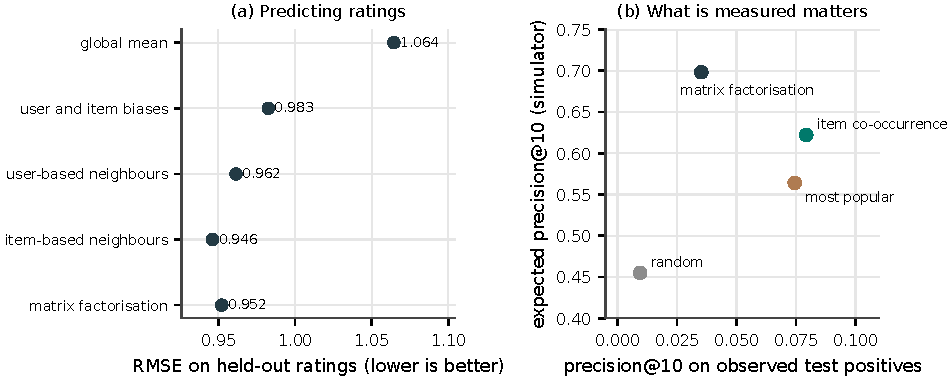
\includegraphics[width=\textwidth]{ch07/recsys_eval}
\caption{(a) Error of five rating predictors on held-out ratings. (b) Precision@10 of four recommenders measured on the observed test positives and, with the
simulator's latent ratings, as the expected share of recommended items that the users would like.}
\label{fig:receval}
\end{figure}

The random split of this experiment measures how well the held-out ratings of known users are
recovered; recommending in the future calls for a split by time, and new users or items need their own protocol.
Offline evaluation has a deeper limitation: it measures how well a recommender predicts what users did when they were shown the
recommendations of the \emph{previous} system. A recommender that suggests something users had never been exposed to cannot get
credit for it offline. The final test is an online experiment (\cref{sec:abtesting}), and because recommendation is a sequence of
decisions with feedback, contextual bandits\index{multi-armed bandit!contextual}\index{multi-armed bandit} (\cref{sec:bandits}) and off-policy\index{off-policy evaluation} evaluation (\cref{lst:ips}) are natural tools.
Recommenders also shape the data they learn from: by showing popular items, they make them more popular, and they can narrow what
each user sees, the \emph{filter bubble}. These feedback loops can increase the homogeneity of what users consume while reducing
the value of the recommendations \citep{chaney2018algorithmic}, which is one more reason to monitor recommenders beyond their
accuracy (\cref{ch:monitoring}).

% =====================================================================
\section{Customer relationship management}\label{sec:crm}

\emph{Customer relationship management\index{customer relationship management (CRM)|textbf}} is the process by which an organisation manages its interactions with its
customers, past, present and potential, using the data it collects about them through every channel: purchases, the
website, the phone, e-mail, social media. Data science turns those data into decisions that improve the relationship
and the business \citep{provost2013data}: whom to target to acquire new customers, what to offer to existing ones
(\emph{cross-selling} and \emph{up-selling}), who is about to leave (\emph{churn}) and is worth retaining, and how much
each customer is worth over the whole relationship (the \emph{customer lifetime value}). Simple summaries of the
behaviour of each customer, such as the \emph{recency}, \emph{frequency} and \emph{monetary} value of their purchases
(RFM), are useful baseline
features in many of these tasks, computed over a stated period before the decision (for acquiring new customers
there may be no history at all).

\subsection{The expected value of a decision}

Most CRM\index{customer relationship management (CRM)} decisions have the same structure: for each customer, decide whether to act (send an offer, call, give a
discount) given a probability estimated by a model and the costs and benefits of each outcome. If contacting a customer
costs $c$, a positive response brings a margin $m$, and the sale would not happen without the contact (so that its
whole margin is due to the contact), contacting them is worth it when the expected value is positive,
\begin{equation}\label{eq:expectedvalue}
  \E[\text{profit}]=p(\text{response}\mid x)\cdot m-c>0
  \quad\Longleftrightarrow\quad
  p(\text{response}\mid x)>\frac{c}{m},
\end{equation}
which is the cost-sensitive\index{cost-sensitive learning} threshold\index{threshold} of \cref{sec:costs} again. If customers may buy anyway, what matters is the increase
caused by the contact: contact when $m\,[P(Y(1)=1\mid x)-P(Y(0)=1\mid x)]>c$, the uplift\index{uplift modelling} of \cref{sec:uplift}. Applying
the rule customer by customer requires calibrated\index{calibration} probabilities (\cref{sec:calibration}): a model that ranks customers
well but overestimates their probabilities will contact too many of them. A profit curve\index{profit curve} computed on labelled
validation data\index{validation set}, as below, uses only the ranking and needs no calibration, but it needs representative data and an
estimate of its uncertainty.

\subsection{Designing a mailing campaign}

Consider a company that sells by catalogue and wants to promote a new product among the customers in its database. Sending
the advertisement to everybody is usually unprofitable. Data science can predict how each customer will respond and use the
predictions to design the campaign\index{mailing campaign} \citep{ling1998data}:
\begin{enumerate}
  \item select a random and sufficiently large sample of customers (a \emph{pilot});
  \item send them the advertisement;
  \item after some time, label each customer of the pilot with 1 if they bought the product and 0 otherwise;
  \item train a probabilistic classifier on the labelled pilot, which estimates the probability that each customer responds;
  \item rank the customers by that probability and draw the \emph{cumulative response curve}, also called the \emph{gains
        chart\index{cumulative gains chart|textbf}}: the share of all the responses obtained as a function of the share of customers contacted;
  \item add the costs and benefits to obtain a \emph{profit curve\index{profit curve|textbf}}, and choose how many customers to contact.
\end{enumerate}
The pilot must be random: only then are its responses a fair sample of how all customers would respond, the same argument
as the hold-out\index{counterfactual hold-out} of \cref{lst:holdout}. Part of the pilot is kept aside to draw the curves, so that the model is not
evaluated on its own training data\index{training set}. The same validation data are then used to choose how many customers to
mail, so the reported maximum is still a development estimate: the chosen model and cutoff should be assessed on
an independent sample, or with a resampling design that repeats the whole selection. The features must describe
the customers before the contact, and the responses must be counted over a completed response window.

\begin{pylisting}[label={lst:crmdata}]{A synthetic customer database and a pilot mailing (file \texttt{crm\_data.py})}
"""A synthetic customer database and a pilot mailing for the CRM examples (Unit 7)."""
import numpy as np

def customers(n=100_000, seed=6):
    rng = np.random.default_rng(seed)
    recency = rng.exponential(120, n)                  # days since the last purchase
    frequency = rng.poisson(3, n)                      # purchases in the last two years
    monetary = rng.gamma(2, 40, n)                     # average order value (EUR)
    age = rng.integers(18, 85, n)
    web = (rng.random(n) < 0.6).astype(int)            # buys online
    logit = (-3.4 - 0.01 * recency + 0.3 * frequency
             + 0.004 * monetary + 0.5 * web - 0.01 * (age - 45))
    X = np.c_[recency, frequency, monetary, age, web]
    # features, true response probability
    return X, 1 / (1 + np.exp(-logit)), rng

def pilot(n_pilot=10_000, seed=6):
    """Mail a random sample; split who responded into training and validation halves."""
    X, p, rng = customers(seed=seed)
    idx = rng.choice(len(p), n_pilot, replace=False)
    y = (rng.random(n_pilot) < p[idx]).astype(int)
    half = n_pilot // 2
    rest = np.setdiff1d(np.arange(len(p)), idx)        # the customers still to be mailed
    return X[idx[:half]], y[:half], X[idx[half:]], y[half:], X[rest], p[rest], rng
\end{pylisting}

\begin{pylisting}[label={lst:mailing}]{Designing a mailing campaign with gains and profit curves}
import numpy as np
from sklearn.ensemble import GradientBoostingClassifier
from sklearn.metrics import roc_auc_score
from crm_data import pilot

X_tr, y_tr, X_val, y_val, X_rest, p_rest, rng = pilot()
print(f"pilot: {len(y_tr) + len(y_val):,} customers mailed, "
      f"response rate {np.r_[y_tr, y_val].mean():.1%}")
model = GradientBoostingClassifier(random_state=0).fit(X_tr, y_tr)
score = model.predict_proba(X_val)[:, 1]
print(f"validation AUC {roc_auc_score(y_val, score):.3f}")
ranked = y_val[np.argsort(-score)]                     # responses in mailing order
gains = np.cumsum(ranked) / ranked.sum()               # share of all responses captured
for f in (0.1, 0.2, 0.5):
    n = int(f * len(ranked))
    print(f"mailing the top {f:.0%}: {gains[n - 1]:.0%} of the responses, "
          f"lift {gains[n - 1] / f:.1f}")

# the campaign: the rest of the base
N = len(p_rest)
share = np.arange(1, len(ranked) + 1) / len(ranked)
CONFIGS = {"config 1": (10_000, 1.50, 30.0), "config 2": (20_000, 0.80, 25.0)}
curves = {}
order_rest = np.argsort(-model.predict_proba(X_rest)[:, 1])   # the real campaign
for name, (fixed, per_mail, margin) in CONFIGS.items():
    mailed = margin * np.cumsum(ranked) * N / len(ranked) - per_mail * share * N - fixed
    profit = np.r_[0.0, mailed]                        # index 0: do not launch at all
    curves[name] = profit
    best = int(np.argmax(profit))
    if best == 0:
        print(f"{name}: do not launch the campaign")
        continue
    n_mail = int(best / len(ranked) * N)
    real = margin * p_rest[order_rest[:n_mail]].sum() - per_mail * n_mail - fixed
    print(f"{name}: mail the top {best / len(ranked):.0%} ({n_mail:,} customers), "
          f"{profit[best]:,.0f} EUR on validation")
    print(f"          true expected profit in the simulation {real:,.0f} EUR; "
          f"mailing everyone {profit[-1]:,.0f} EUR")
\end{pylisting}
\begin{pyoutput}
pilot: 10,000 customers mailed, response rate 6.9%
validation AUC 0.740
mailing the top 10%: 29% of the responses, lift 2.9
mailing the top 20%: 44% of the responses, lift 2.2
mailing the top 50%: 82% of the responses, lift 1.6
config 1: mail the top 55% (49,860 customers), 78,290 EUR on validation
          true expected profit in the simulation 75,243 EUR; mailing everyone 42,380 EUR
config 2: mail the top 70% (62,909 customers), 76,372 EUR on validation
          true expected profit in the simulation 75,715 EUR; mailing everyone 64,150 EUR
\end{pyoutput}

\Cref{lst:crmdata} creates a database of 100,000 customers whose probability of buying depends on their recency, frequency,
monetary value, age and channel. In \cref{lst:mailing}, a pilot of 10,000 customers responds at a rate of 6.9\%. A gradient
boosting\index{gradient boosting}\index{boosting} model trained on half of the pilot has an AUC\index{area under the ROC curve (AUC)} of 0.740 on the other half; the AUC measures its ranking and says nothing about the calibration of its
probabilities. Its gains are substantial
(\cref{fig:campaign}a): mailing the 10\% of customers with the highest scores captures 29\% of all the responses, a
\emph{lift\index{lift|textbf}} of 2.9 over mailing at random, and mailing the top half captures 82\% of them.

The profit curve depends on the costs. The listing compares two configurations:
\begin{itemize}
  \item configuration 1: an initial cost of 10,000~EUR, 1.50~EUR per brochure and a margin of 30~EUR per sale;
  \item configuration 2: an initial cost of 20,000~EUR, 0.80~EUR per brochure and a margin of 25~EUR per sale.
\end{itemize}
With the first, the best decision is to mail the top 55\% of the remaining 90,000 customers, for an estimated profit of
78,290~EUR, while mailing everyone would earn only 42,380~EUR, also estimated on the validation data. With the second, cheaper per brochure, it pays to mail more
customers, the top 70\%, for an estimated 76,372~EUR (\cref{fig:campaign}b). The estimates, computed from 5,000 validation
customers and scaled to the whole database, are close to the simulation's true expected profits of the selected
campaigns (75,243 and 75,715~EUR), which a real company would not know; the cost of the pilot comes on top. The
curves also include not launching at all, with a profit of 0 while the fixed cost can still be avoided: when every
campaign loses money, the best decision is to mail nobody. If the fixed cost has already been paid, it is sunk: it is the
same for every option, so it should be left out of the comparison, and mailing nobody then has an incremental profit of 0. The two configurations end up with similar profits but very different campaigns, which is why the costs must be part of the design from the start.

\begin{figure}[htbp]
\centering
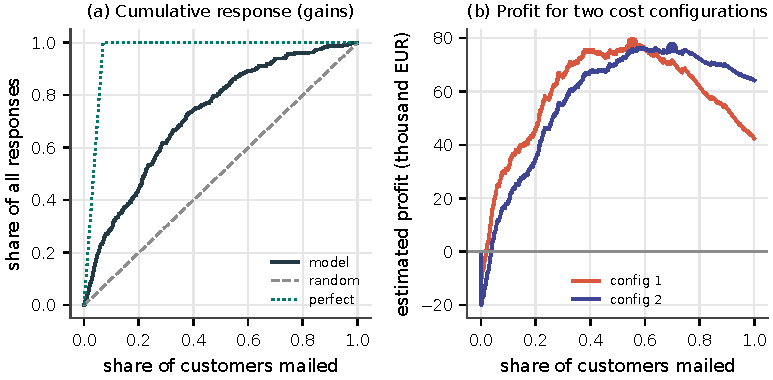
\includegraphics[width=\textwidth]{ch07/campaign}
\caption{(a) Cumulative response curve of the response model, with random and perfect targeting. (b) Profit estimated on the
validation data as a function of the share of customers mailed, for two cost configurations; the point at 0 is
not launching, and the dots mark the decisions selected on the same data.}
\label{fig:campaign}
\end{figure}

\subsection{Uplift modelling}\label{sec:uplift}

The campaign\index{mailing campaign} above targets the customers most likely to buy \emph{after receiving the brochure}. But some of them would
have bought anyway, and the brochure was wasted on them. What matters is the effect of the contact, the difference between
the probability of buying if contacted and if not contacted, which is a causal quantity: the conditional average treatment effect
$\mathrm{CATE}(x)=\E[Y_1-Y_0\mid X=x]$ of the contact (\cref{sec:potentialoutcomes}). Customers
fall into four groups \citep{radcliffe2011real}:
\begin{itemize}
  \item \emph{persuadables\index{uplift modelling!persuadables and sleeping dogs|textbf}}, who buy only if contacted: the only group in which the campaign creates sales (whether they pay for the contact
        is another question);
  \item \emph{sure things}, who buy whether contacted or not: contacting them wastes money;
  \item \emph{lost causes}, who do not buy either way;
  \item \emph{sleeping dogs}, who buy less if contacted, for instance because the contact reminds them to cancel a
        subscription or annoys them: contacting them destroys value.
\end{itemize}
These types are defined by the two potential outcomes of the same customer (\cref{sec:causality}), and only one of
them is ever observed, so the type of an individual cannot be identified. For instance, a population made of half sure things
and half lost causes and another made of half persuadables and half sleeping dogs have the same average effect:
zero. What data can reveal are segments of customers with positive or negative average effects.
A response model ranks sure things and persuadables at the top, and sleeping dogs too if they buy often. \emph{Uplift\index{uplift modelling|textbf}
modelling} estimates the effect instead,
\begin{equation}
  \tau(x)=\E\bigl[Y(1)-Y(0)\mid X=x\bigr],
\end{equation}
the conditional average treatment effect of the contact. In a randomised campaign, it equals the
difference between the response rates of contacted and non-contacted customers with features $x$. This is why uplift modelling needs data from a randomised campaign, in which a random control
group was not contacted, as in an A/B test\index{A/B testing} (\cref{sec:abtesting}). The simplest method trains two models, one on the
contacted customers and one on the control group, and subtracts their predictions; other methods transform the target so
that a single model can be used \citep{jaskowski2012uplift}, or build trees that split directly on differences in uplift
\citep{radcliffe2011real,gutierrez2017causal}. Because the effect of the contact on an individual customer is never observed,
uplift models are evaluated with \emph{uplift} or \emph{Qini curves}, which compare the response rates of the treated and
control customers among those ranked highest \citep{radcliffe2007using}.

\begin{pylisting}[label={lst:uplift}]{A response model against an uplift model on a randomised campaign}
import numpy as np
from sklearn.ensemble import GradientBoostingClassifier

rng = np.random.default_rng(7)
n = 40_000
age, freq, web = rng.integers(18, 85, n), rng.poisson(3, n), rng.random(n) < 0.6
p0 = 1 / (1 + np.exp(-(-3.5 + 0.45 * freq + 0.3 * web)))      # buys without contact
positive_seg = (age < 35) & (freq <= 2)          # contact raises the purchase rate
negative_seg = (age >= 60) & (freq >= 5)          # contact lowers it
# the effect of the contact on the probability of buying
tau = np.where(positive_seg, 0.08, np.where(negative_seg, -0.06, 0.005))
X = np.c_[age, freq, web]
T = rng.random(n) < 0.5                                         # a randomised campaign
y = (rng.random(n) < np.clip(p0 + T * tau, 0, 1)).astype(int)
train, test = np.arange(n) < n // 2, np.arange(n) >= n // 2

gb = lambda: GradientBoostingClassifier(random_state=0)
# classic: who buys if mailed
response = gb().fit(X[train & T], y[train & T])
m1, m0 = gb().fit(X[train & T], y[train & T]), gb().fit(X[train & ~T], y[train & ~T])
scores = {"random": rng.random(n), "response model": response.predict_proba(X)[:, 1],
          "uplift (two models)": m1.predict_proba(X)[:, 1] - m0.predict_proba(X)[:, 1]}
idx = np.flatnonzero(test)
print("top 20% by             true effect   estimated [95% CI]      + segment  - segment")
for name, s in scores.items():
    top = idx[np.argsort(-s[idx])[: len(idx) // 5]]            # the targeted customers
    treated, control = top[T[top]], top[~T[top]]               # randomised, so comparable
    effect = y[treated].mean() - y[control].mean()
    se = np.sqrt(y[treated].var(ddof=1) / len(treated)
                 + y[control].var(ddof=1) / len(control))
    lo, hi = 1000 * (effect - 1.96 * se), 1000 * (effect + 1.96 * se)
    print(f"{name:22s} {1000 * tau[top].mean():+7.1f}   {1000 * effect:+7.1f} "
          f"[{lo:+6.1f}, {hi:+6.1f}]      {positive_seg[top].mean():4.0%}      "
          f"{negative_seg[top].mean():4.0%}")
\end{pylisting}
\begin{pyoutput}
top 20% by             true effect   estimated [95% CI]      + segment  - segment
random                    +8.2     +13.9 [  -8.1,  +35.9]       11%        7%
response model            -9.2     -12.5 [ -41.1,  +16.0]        1%       23%
uplift (two models)      +32.8     +43.8 [ +21.0,  +66.5]       38%        1%
\end{pyoutput}

\Cref{lst:uplift} simulates a randomised campaign of 40,000 customers. The contact raises the probability of buying
by 0.08 in an observable segment of young, infrequent buyers, lowers it by 0.06 in a segment of older, very frequent
buyers, and changes it by 0.005 for everybody else; these segments, not individual persuadables or sleeping dogs, are
what the simulation defines. Contacting a random 20\% of the test customers produces 8.2 extra sales per 1000 contacts
(the true expected effect in the simulation). A response model, which ranks the customers who are most likely to buy
when contacted, does worse than random: it \emph{loses} 9.2 sales per 1000 contacts, because 23\% of the customers it
selects belong to the negative-effect segment (frequent buyers, likely to buy anyway) and only 1\% to the positive one.
The uplift model creates 32.8 extra sales per 1000 contacts, four times as many as random targeting, with 38\% of its
targets in the positive-effect segment and 1\% in the negative one (\cref{fig:uplift}). A real campaign does not know
these true effects, but its randomised design allows them to be \emph{estimated}. Comparing the contacted and the
control customers among those selected by each ranking gives +13.9, $-12.5$ and +43.8 extra sales per 1000 contacts. Their 95\% confidence intervals\index{confidence interval} go from $-8.1$ to +35.9, from $-41.1$ to +16.0 and from +21.0 to +66.5, so only the effect of
the uplift model is clearly positive. Whether it pays is another question: with a margin of 30~EUR and 1.50~EUR per
brochure, 32.8 extra sales per 1000 contacts bring $30\cdot0.0328-1.50\approx-0.52$~EUR per contact. At a 20\% contact
rate, even uplift targeting has a negative expected profit at these prices, and the right decision would be not to launch, or to contact fewer customers
with a larger effect: customers should be ranked by their expected incremental profit, $m\,\tau(x)-c$.

\begin{figure}[htbp]
\centering
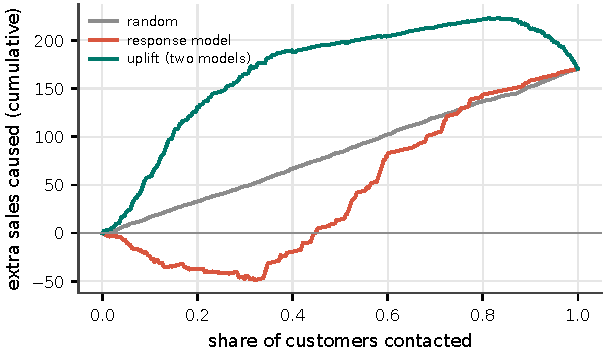
\includegraphics[width=0.72\textwidth]{ch07/uplift}
\caption{Extra sales caused by contacting the customers ranked highest by each score (the true effects of the simulation),
as a function of the share of customers contacted.}
\label{fig:uplift}
\end{figure}

\begin{keyidea}
To decide whom to act on, model the \emph{effect} of the action. Predicting who will buy, churn or recover
answers a different question from predicting whom the offer, the retention call or the treatment will change, and the action creates value only for the customers it changes.
\end{keyidea}

\subsection{Churn and customer lifetime value\extsec}\label{sec:churn}

Customers who leave take their future purchases with them. Predicting \emph{churn\index{churn|textbf}},
which customers are about to leave, is a common CRM\index{customer relationship management (CRM)} task,
and \citet{provost2013data} use it as a running example. A churn model is built like the response model
of the campaign, with three differences:
\begin{itemize}
\item \emph{time}: the features describe each customer at a reference date, from the data of an
\emph{observation window} before it, and the target says whether the customer left during a
\emph{prediction window} after it (for instance, the next three months). Features recorded after the
reference date, such as a request to cancel, leak the answer (\cref{sec:protocols}), and the model must
be evaluated on reference dates later than those used to train it;
\item \emph{value}: losing a customer who spends little costs less than losing one who spends a lot.
The \emph{customer lifetime value\index{customer lifetime value|textbf}} (CLV) estimates the margin that
a customer will bring over the rest of the relationship; with a yearly margin $m$, a probability $r$ of
staying each year and a discount rate $d$, over $T$ years,
\begin{equation}\label{eq:clv}
\mathrm{CLV}=\sum_{t=1}^{T}\frac{m\,r^t}{(1+d)^t},
\end{equation}
and the expected loss from a customer is their probability of leaving times their value;
\item \emph{the action}: a retention offer is a contact like the brochure of the campaign, so the
reasoning of \cref{sec:uplift} applies. The offer creates value only for the customers it keeps, and it
can wake sleeping dogs\index{uplift modelling!persuadables and sleeping dogs}, customers who had not
thought of leaving until the offer reminded them of their contract. A retention campaign therefore needs
a randomised control group, and it should rank customers by the value that the offer saves,
$\tau(x)\,\mathrm{CLV}(x)-c$, where $\tau(x)$ is the reduction in the probability of leaving caused by
the offer and $c$ its cost.
\end{itemize}

% =====================================================================
\section{Interactive applications with Shiny}\label{sec:shinyapps}

A model is only useful if the people who must act on it can use it. A marketing manager will not run a Python script to
decide how many brochures to send, but will happily move a slider in a web page and watch the profit curve\index{profit curve} change.
\emph{Shiny\index{Shiny|textbf}} builds such interactive web applications from code alone \citep{shiny2012,wickham2021mastering}. It was born in the
R community, where RStudio (now Posit) released it as open source in 2012, and Posit also maintains Shiny for Python
\citep{shinypython2024}, which we use here (\cref{tab:shiny}). It communicates with the browser through WebSockets, is built on
a \emph{reactive\index{reactive programming|textbf} programming} model, and can be extended with custom inputs and outputs. We introduced it in
\cref{sec:webapps}; here we look at how it works.

\subsection{The parts of an application}

A Shiny\index{Shiny} application has three components: a \emph{user interface} object, which defines the layout and appearance of the
application; a \emph{server function}, which contains the instructions to build its outputs; and a call that creates the
application from the pair, \texttt{App(app\_ui, server)}. The three usually live in a single file, \texttt{app.py}, which is
launched with \texttt{shiny run app.py}; adding \texttt{-{}-reload} restarts the application whenever the code is saved, which is
convenient while developing it. Shiny for Python also offers \emph{Shiny Express}, a more concise syntax in which the interface and
the outputs are written together, in the order in which they appear on the page.

The user interface is built by nesting functions. \emph{Layout} functions organise the page: a fluid page adapts to the size
of the browser window, and a sidebar layout places the controls in a side panel and the results in a main panel. Static
content (titles, paragraphs, images) is added with functions that mirror the HTML tags. \emph{Control widgets} (sliders, select
boxes, check boxes, numeric and text inputs, date ranges, file uploads, buttons) collect values from the user; the first
two arguments of every widget are an identifier, used to read its value in the server, and a label shown to the user.
\emph{Outputs} (texts, tables, plots, images, HTML) are reserved in the interface with an output function and an identifier,
and built in the server by the matching \emph{render} function, in two steps: add the output to the interface, and tell the
server how to build it.

\subsection{Reactivity}\label{sec:reactivity}

The server never says \emph{when} to recompute an output. An output becomes \emph{reactive\index{reactive programming|textbf}} as soon as the code that builds
it reads the value of an input: Shiny\index{Shiny} records the dependency and, whenever that input changes, re-runs the code and sends the
new output to the browser. The dependencies form a \emph{reactive graph} (\cref{fig:reactivegraph}).

Re-running too much makes applications slow. If an output reads a data set from a remote service and then plots it on a
logarithmic scale chosen with a check box, ticking the box downloads the data again, although only the scale changed. The
solution is a \emph{reactive expression}: a piece of code that reads some inputs and returns a value, created with
the \texttt{@reactive.calc} decorator. Reactive expressions \emph{cache} their value:
the first call computes and stores it, later calls return the stored value, and only when one of the inputs it read changes is
the value marked as obsolete and recomputed at the next call. Expensive steps (loading data, training a model) go in reactive
expressions that depend only on the inputs that affect them, and the outputs call those expressions.

\begin{figure}[htbp]
\centering
\begin{tikzpicture}[font=\scriptsize\sffamily,
  inp/.style={draw=edmteal,fill=edmteal!12,rounded corners=2pt,minimum height=6.5mm,minimum width=24mm,align=center},
  calc/.style={draw=edmgold,fill=edmgold!25,rounded corners=2pt,minimum height=9mm,minimum width=30mm,align=center},
  outp/.style={draw=edmnavy,fill=edmnavy!8,rounded corners=2pt,minimum height=6.5mm,minimum width=27mm,align=center},
  arr/.style={-{Stealth[length=1.5mm]},edmnavy!80}]
  \node[inp] (m) at (0,1.6) {\texttt{model}};
  \node[inp] (f) at (0,0.6) {\texttt{fixed}};
  \node[inp] (c) at (0,-0.4) {\texttt{per\_mail}};
  \node[inp] (g) at (0,-1.4) {\texttt{margin}};
  \node[calc] (r) at (3.9,1.6) {\texttt{ranked()}\\trains and scores (cached)};
  \node[outp] (o1) at (8.2,1.6) {response curve};
  \node[outp] (o2) at (8.2,0.3) {profit curve};
  \node[outp] (o3) at (8.2,-0.9) {summary text};
  \draw[arr] (m) -- (r);
  \draw[arr] (r) -- (o1);
  \draw[arr] (r) -- (o2);
  \draw[arr] (r) -- (o3);
  \foreach \x in {f,c,g} { \draw[arr] (\x.east) -- (o2.west); \draw[arr] (\x.east) -- (o3.west); }
  \node[font=\tiny\sffamily,text=edmteal] at (0,2.25) {inputs};
  \node[font=\tiny\sffamily,text=edmbronze] at (3.9,2.35) {reactive expression};
  \node[font=\tiny\sffamily,text=edmnavy] at (8.2,2.25) {outputs};
\end{tikzpicture}
\caption{The reactive graph of the campaign planner: changing a cost re-runs only the profit curve and the summary; changing
the model retrains it once and updates every output. Each session has its own \texttt{ranked()} and cache.}
\label{fig:reactivegraph}
\end{figure}

Where code is placed also determines how often it runs:
\begin{itemize}
  \item code at the top level of the module, outside the server function (importing libraries, reading data sets, loading
        models), runs once per Python process, when the
        application starts, and is shared by the sessions that the process serves (with several workers or
        replicas, each process loads its own copy);
  \item code inside the server function but outside any render function runs \emph{once per user session}: the place for objects
        that each user needs their own copy of;
  \item code inside a render function runs \emph{every time} an input it reads changes, possibly many times a second while a user
        drags a slider, so it should contain only what must be recomputed to build that output.
\end{itemize}
\Cref{lst:placementapp} marks the three places in a small application, and \cref{lst:placement} measures them by connecting two
users to it: the top-level code runs once, the server function once per user, and the render function every time the slider
moves.

\begin{pylisting}[label={lst:placementapp}]{Three places for code in a Shiny for Python application (file \texttt{placement\_app.py})}
from shiny import App, render, ui

RUNS = {"top level": 0, "server": 0, "render": 0}        # how often each part runs

RUNS["top level"] += 1             # runs once, when the application starts:
CATALOGUE = list(range(1, 1001))   # load data, models and libraries here

app_ui = ui.page_fluid(ui.input_slider("n", "Products", 1, 1000, 10),
                       ui.output_text("total"))

def server(input, output, session):
    RUNS["server"] += 1            # runs once per user session:
    basket = []                    # objects that each user needs their own copy of

    @render.text
    def total():
        RUNS["render"] += 1        # runs every time an input it reads changes
        return f"Total of the first {input.n()} products: {sum(CATALOGUE[:input.n()])}"

app = App(app_ui, server)
\end{pylisting}

\begin{pylisting}[label={lst:placement}]{How often each part runs, measured with two simulated users}
from concurrent.futures import ThreadPoolExecutor
import json
from starlette.testclient import TestClient
import placement_app as pa

_POOL = ThreadPoolExecutor(max_workers=1)

def read_output(ws, name="total", seconds=30, max_messages=50):
    """Read server messages until the value of an output arrives. The blocking read runs
    in a worker thread, so the time limit works on any platform and in any thread."""
    for _ in range(max_messages):
        message = json.loads(_POOL.submit(ws.receive_text).result(timeout=seconds))
        if name in message.get("values", {}):
            return message["values"][name]
    raise RuntimeError(f"output {name} never arrived")


def start(ws, n=10):
    ws.send_text(json.dumps({"method": "init", "data": {
        "n": n, ".clientdata_output_total_hidden": False}}))
    return read_output(ws)

with TestClient(pa.app) as client:
    print(f"application started:                  {pa.RUNS}")
    with client.websocket_connect("/websocket/") as user1:
        start(user1)
        print(f"user 1 opens the page:                {pa.RUNS}")
        for n in (50, 200, 1000):                 # user 1 drags the slider
            user1.send_text(json.dumps({"method": "update", "data": {"n": n}}))
            answer = read_output(user1)
        print(f"user 1 moves the slider three times:  {pa.RUNS}")
        with client.websocket_connect("/websocket/") as user2:
            start(user2)
            print(f"user 2 opens the page:                {pa.RUNS}")
print(f"user 1 sees: {answer}")
\end{pylisting}
\begin{pyoutput}
application started:                  {'top level': 1, 'server': 0, 'render': 0}
user 1 opens the page:                {'top level': 1, 'server': 1, 'render': 1}
user 1 moves the slider three times:  {'top level': 1, 'server': 1, 'render': 4}
user 2 opens the page:                {'top level': 1, 'server': 2, 'render': 5}
user 1 sees: Total of the first 1000 products: 500500
\end{pyoutput}

\subsection{The campaign planner}

\Cref{lst:crmapp} turns the mailing\index{mailing campaign} campaign of \cref{sec:crm} into an application, including the model selector that is a
classic exercise: the user chooses a model (a decision tree\index{decision tree}, a random forest\index{random forest} or nearest neighbours\index{k-nearest neighbours@$k$-nearest neighbours}) and the three costs, and sees
the cumulative response curve, the profit curve\index{profit curve} and a sentence with the best decision. The data are loaded once, outside the server.
Training and scoring happen in the reactive\index{reactive programming} expression \texttt{ranked()}, which depends only on the chosen model, so moving a cost
slider redraws the profit curve and updates the sentence without retraining anything. Each session has its own
\texttt{ranked()}, which caches (stores) the current result until the model changes. This has two limitations. Returning to a model chosen before trains it
again; a cache keyed by the model and the version of the data would avoid this. And training inside the reactive
expression blocks the process while it runs. When training is slow, pretrain the models, or send the work to an
executor (a separate process for CPU-bound Python code) or to a training service, coordinated by an \texttt{ExtendedTask}. An \texttt{ExtendedTask} on its own does not move CPU-bound work off the thread that runs the event loop \citep{shinypython2024}. Rapid movements of a slider may
also be grouped into fewer updates, and the global log of trainings is instrumentation for this demonstration, not an
audit log. The sentence also considers not launching the campaign at all.

\begin{pylisting}[label={lst:crmapp}]{The campaign planner, with a cached reactive expression (file \texttt{crm\_app.py}; run it with \texttt{shiny run crm\_app.py})}
import matplotlib.pyplot as plt
import numpy as np
from shiny import App, reactive, render, ui
from sklearn.ensemble import RandomForestClassifier
from sklearn.neighbors import KNeighborsClassifier
from sklearn.pipeline import make_pipeline
from sklearn.preprocessing import StandardScaler
from sklearn.tree import DecisionTreeClassifier
from crm_data import pilot

X_train, y_train, X_val, y_val, X_rest, _, _ = pilot()   # loaded once per Python process
N = len(X_rest)                                          # customers in the campaign
MODELS = {"Decision tree": lambda: DecisionTreeClassifier(max_depth=5, random_state=0),
          "Random forest": lambda: RandomForestClassifier(200, min_samples_leaf=20,
                                                          random_state=0),
          "Nearest neighbours": lambda: make_pipeline(StandardScaler(),
                                                     KNeighborsClassifier(100))}
TRAININGS = []                                           # a log, to see the caching

def profit_curve(ranked, fixed, per_mail, margin, n=N):
    """Profit of not launching (index 0) and of mailing the top k customers, for every k,
    scaled to n customers; the fixed cost is paid only if the campaign is launched."""
    ranked = np.asarray(ranked)
    share = np.arange(1, len(ranked) + 1) / len(ranked)
    mailed = margin * np.cumsum(ranked) * n / len(ranked) - per_mail * share * n - fixed
    return np.r_[0.0, mailed]

def decision(profit, n_validation):
    """The best action: not launching (index 0) or mailing the top customers."""
    best = int(np.argmax(profit))
    if best == 0:
        return "Do not launch the campaign: every mailing loses money"
    return (f"Mail the top {best / n_validation:.0%} of {N:,} customers: "
            f"profit {profit[best]:,.0f} EUR")

app_ui = ui.page_sidebar(
    ui.sidebar(
        ui.input_select("model", "Model", list(MODELS)),
        ui.input_slider("fixed", "Initial cost (EUR)", 0, 40_000, 10_000, step=1_000),
        ui.input_slider("per_mail", "Cost per brochure (EUR)", 0.1, 3.0, 1.5, step=0.1),
        ui.input_slider("margin", "Profit per sale (EUR)", 5, 60, 30),
    ),
    ui.output_text("summary"),
    ui.layout_columns(ui.output_plot("response"), ui.output_plot("profit_plot")),
    title="Mailing campaign planner",
)

def server(input, output, session):
    @reactive.calc                     # cached: recomputed only when the model changes
    def ranked():
        TRAININGS.append(input.model())
        model = MODELS[input.model()]().fit(X_train, y_train)
        return y_val[np.argsort(-model.predict_proba(X_val)[:, 1])]

    def profit():
        return profit_curve(ranked(), input.fixed(), input.per_mail(), input.margin())

    @render.text
    def summary():
        return decision(profit(), len(ranked()))

    @render.plot
    def response():
        r = ranked()
        x = np.arange(1, len(r) + 1) / len(r)
        fig, ax = plt.subplots()
        ax.plot(x, np.cumsum(r) / r.sum(), label=input.model())
        ax.plot([0, 1], [0, 1], "--", label="random")
        ax.set(xlabel="share of customers mailed", ylabel="share of responses")
        ax.legend()
        return fig

    @render.plot(alt="Profit curve")
    def profit_plot():
        p = profit()
        fig, ax = plt.subplots()
        ax.plot(np.arange(len(p)) / (len(p) - 1), p)        # 0: not launching
        ax.axhline(0, color="grey")
        ax.set(xlabel="share of customers mailed", ylabel="profit (EUR)")
        return fig

app = App(app_ui, server)                                # run: shiny run crm_app.py
\end{pylisting}

The behaviour that matters can be tested automatically, as in \cref{sec:webapps}. \Cref{lst:crmtest} checks the profit
computation, including the decision not to launch, against small cases worked out by hand, checks that the page contains every control and output, and then connects to
the application as a browser would, through its WebSocket protocol. It changes the cost per brochure, checks that the sentence
changes and that the model was \emph{not} retrained (the application keeps a log of its trainings), then changes the model and checks
that it was retrained exactly once. With a decision tree and the costs of the first configuration, the application recommends mailing
the top 71\% of the 90,000 customers, for a profit of 69,515~EUR; at 0.50~EUR per brochure, it recommends 84\%, for 135,368~EUR. These tests
check the arithmetic, the identifiers of the page and the reactive behaviour of the server through its WebSocket
protocol; they do not exercise the rendering in a browser or its JavaScript, which a browser test, for instance
with Playwright, can check, together with both plots. The helper that reads the outputs gives up after 50 messages,
and a time limit stops a regression from blocking the test run forever. The blocking read runs in a worker thread with a
timeout, which works on any operating system and in any thread; an alarm signal would work only on Unix, in the main thread,
and would replace the handler of the whole process. The test client speaks the internal protocol of
Shiny\index{Shiny}, which may change between versions, so the requirements file pins them (here Shiny 1.8.0, Starlette 1.7.0 and
pytest 9.1.1).

\begin{pylisting}[label={lst:crmtest}]{Testing the planner: profit, page, and reactive caching (file \texttt{test\_crm\_app.py}; run it with \texttt{pytest})}
from concurrent.futures import ThreadPoolExecutor
import json

import numpy as np
import pytest
from starlette.testclient import TestClient
import crm_app

@pytest.fixture(scope="module")
def client():
    with TestClient(crm_app.app) as c:
        yield c

_POOL = ThreadPoolExecutor(max_workers=1)

def read_output(ws, name="summary", seconds=30, max_messages=50):
    """Read server messages until the value of an output arrives. The blocking read runs
    in a worker thread, so the time limit works on any platform and in any thread."""
    for _ in range(max_messages):
        message = json.loads(_POOL.submit(ws.receive_text).result(timeout=seconds))
        if name in message.get("values", {}):
            return message["values"][name]
    raise AssertionError(f"output {name} never arrived")


def test_profit_curve():                     # unit tests, computed by hand
    p = crm_app.profit_curve(np.array([1, 0, 1, 0]), fixed=10, per_mail=1, margin=5, n=4)
    assert np.allclose(p, [0, -6, -7, -3, -4])     # index 0: do not launch
    assert crm_app.decision(p, 4).startswith("Do not launch")
    p = crm_app.profit_curve(np.array([1, 0, 1, 0]), fixed=1, per_mail=1, margin=5, n=4)
    assert crm_app.decision(p, 4).startswith("Mail the top 75%")

def test_page_has_the_controls(client):
    page = client.get("/").text
    for name in ("model", "fixed", "per_mail", "margin", "summary", "response",
                 "profit_plot"):
        assert f'id="{name}"' in page

def test_costs_do_not_retrain_but_the_model_does(client):
    crm_app.TRAININGS.clear()
    with client.websocket_connect("/websocket/") as ws:
        ws.send_text(json.dumps({"method": "init", "data": {
            "model": "Decision tree", "fixed": 10_000, "per_mail": 1.5, "margin": 30,
            ".clientdata_output_summary_hidden": False}}))
        first = read_output(ws)
        ws.send_text(json.dumps({"method": "update", "data": {"per_mail": 0.5}}))
        cheaper = read_output(ws)
        assert cheaper != first and crm_app.TRAININGS == ["Decision tree"]
        new_model = {"model": "Nearest neighbours"}
        ws.send_text(json.dumps({"method": "update", "data": new_model}))
        read_output(ws)
        assert crm_app.TRAININGS == ["Decision tree", "Nearest neighbours"]
    print(f"\n  1.50 EUR per brochure: {first}\n  0.50 EUR per brochure: {cheaper}")
\end{pylisting}
\begin{pyoutput}
============================= test session starts ==============================
collecting ... collected 3 items

test_crm_app.py::test_profit_curve PASSED
test_crm_app.py::test_page_has_the_controls PASSED
test_crm_app.py::test_costs_do_not_retrain_but_the_model_does 
  1.50 EUR per brochure: Mail the top 71% of 90,000 customers: profit 69,515 EUR
  0.50 EUR per brochure: Mail the top 84% of 90,000 customers: profit 135,368 EUR
PASSED

============================== 3 passed in 2.76s ===============================
\end{pyoutput}

\subsection{Sharing applications}

There are several ways of sharing a Shiny\index{Shiny} for Python application. The simplest is to share its code, for instance in a Git\index{Git}
repository: users install the packages listed in its requirements file and launch it with \texttt{shiny run}. \emph{Shinylive\index{Shinylive|textbf}}
exports the application to a set of static files that run entirely in the user's browser, with Python compiled to
WebAssembly, so that it can be published on any web server, or even shared as a link, with no Python server behind it; the price is
that the code and the data travel to the browser, and not every package is available. To host the application as a web service that
anyone can open, it can be deployed to \emph{Posit Connect Cloud\index{Posit Connect Cloud|textbf}}, Posit's hosting service, for instance
directly from a Git repository with a requirements file, or to \emph{Posit Connect}, its platform for an organisation's
own infrastructure, which adds authentication, encrypted connections and administration tools. Posit is migrating
its older service, shinyapps.io, to Connect Cloud during 2027 \citep{posit2026connectcloud}, so new applications should
follow the current deployment documentation; or it can be packaged in a container\index{containers} and run like any other web service (\cref{sec:packaging}).

% =====================================================================
% ---------------------------------------------------------------------
\section{The applications across the life cycle}\label{sec:applifecycle}

The two applications of this unit go through every stage of the life cycle described in the
introduction, and each stage uses the tools of an earlier unit. \Cref{tab:applifecycle} follows a
recommender and a customer campaign (a response, uplift or churn model) from evaluation to updating.

\begin{table}[htbp]
\centering\small
\caption{A recommender and a customer campaign through the life cycle of a model.}\label{tab:applifecycle}
\begin{tabularx}{\textwidth}{@{}>{\raggedright\arraybackslash}p{1.6cm}>{\raggedright\arraybackslash}X>{\raggedright\arraybackslash}X@{}}
\toprule
Stage & Recommender & Customer campaign\\
\midrule
Evaluate & ranking metrics on a split by time, with coverage and novelty, against a popularity baseline
(\cref{sec:receval}) & AUC and gains on a held-out part of the pilot; profit curve on validation data,
confirmed on a separate test set (\cref{sec:crm})\\
Decide & how many items to show and where; filters for items already bought, unavailable or not allowed &
whom to contact, by expected incremental profit, $m\,\tau(x)-c$, or by the value that a retention offer
saves (\cref{sec:uplift,sec:churn})\\
Deploy & candidates precomputed in batch and ranked at request time within a latency budget
(\cref{sec:deployoptions}) & batch scoring of the customer base before each campaign, and a planner for
the people who decide (\cref{sec:shinyapps})\\
Monitor & click-through and conversion, coverage, the share of recommendations taken by the most popular
items, drift of the catalogue and of the users (\cref{ch:monitoring}) & response and uplift in a random
control group kept in every campaign, drift of the customer features, calibration of the probabilities\\
Update & frequent retraining as items and users arrive; new versions through A/B tests or interleaving,
and bandits for short-lived content (\cref{sec:abtesting,sec:bandits}) & retraining with the randomised
results of each campaign, so that each campaign also evaluates the current model\\
\bottomrule
\end{tabularx}
\end{table}

Both applications create their own future data. A recommender decides which items users see, so its logs
over-represent what it recommended; a campaign decides whom to contact, so the responses of the customers
it skipped are never observed. In both cases a small share of randomised decisions, logged with their
probabilities (\cref{lst:ips}), keeps the data usable for evaluating the next model, at a cost that can be
estimated in advance, as for the hold-out of \cref{lst:holdout}. In both cases, too, the decision depends on
costs and constraints that change more often than the model: prices, margins, budgets and the items that
cannot be recommended belong in the application, where the people who decide can change them, as in the
planner of \cref{lst:crmapp}.

\section{Summary}\label{sec:summary7}

\begin{itemize}
  \item Recommender systems\index{recommender system} suggest items from interactions (collaborative filtering\index{collaborative filtering}), from item descriptions (content-based\index{content-based filtering}
        filtering) or from both (hybrids).
  \item User-based\index{collaborative filtering!user-based} collaborative filtering predicts ratings as similarity\index{similarity measure}-weighted averages of the ratings of similar users;
        item-based\index{collaborative filtering!item-based} filtering compares items instead, which is more stable and scales better. Similarities computed on few common
        items are unreliable.
  \item Matrix factorisation\index{matrix factorisation} represents users and items by latent factors; it was central to the Netflix\index{Netflix Prize} Prize, whose data also
        showed that anonymised ratings can identify people.
  \item Content-based filtering solves the cold start\index{cold start} of new items and gives explainable\index{explainability} recommendations, but tends to
        overspecialise.
  \item Rating errors evaluate rating prediction, and ranking metrics evaluate recommendation lists; the candidate set, the
        relevance labels and the process that decides what is observed must be stated, because ratings are missing not
        at random. Coverage\index{coverage}, novelty\index{novelty} and diversity\index{diversity!of recommendations} complement accuracy, popularity is a strong baseline, and online
        experiments give the final assessment.
  \item In CRM\index{customer relationship management (CRM)}, decisions follow the expected incremental value of acting, which combines the change that the action causes
        with its costs and benefits; not acting is always one of the options. A mailing\index{mailing campaign} campaign is designed with a random pilot, a probabilistic classifier, a cumulative response curve and a
        profit curve\index{profit curve}, whose optimum depends on the costs.
  \item Uplift\index{uplift modelling} modelling targets the customers whose behaviour the action changes; a response model can do worse than random by
        targeting sure things\index{uplift modelling!persuadables and sleeping dogs} and sleeping dogs.
\item Churn models need features observed before a reference date and a target observed after it, a
temporal evaluation, and a ranking by the value that the retention offer saves; retention offers, like
any contact, can wake sleeping dogs.
  \item Shiny\index{Shiny} builds interactive applications from a user interface and a reactive\index{reactive programming} server; reactive expressions cache expensive
        computations, and the placement of code determines how often it runs.
\item Both applications go through the whole life cycle: offline evaluation, a decision rule with costs,
batch or online deployment, monitoring with a randomised control share, and updates through experiments.
\end{itemize}

\section*{Bibliographic notes}
\phantomsection\addcontentsline{toc}{section}{Bibliographic notes}

\citet{segaran2007programming} is a practical introduction to collaborative filtering\index{collaborative filtering}, and \citet{aggarwal2016recommender} and
\citet{ricci2022recommender} cover recommender systems\index{recommender system} in depth. \citet{koren2009matrix} explain matrix factorisation\index{matrix factorisation} as used in the
Netflix\index{Netflix Prize} Prize, \citet{herlocker2004evaluating} the evaluation of collaborative filtering, and \citet{kaminskas2016diversity} the measures
beyond accuracy. \citet{provost2013data} present the expected value framework, cumulative response and profit curves\index{profit curve} for business
problems, and \citet{gutierrez2017causal} review uplift\index{uplift modelling} modelling. \citet{wickham2021mastering} is a reference on Shiny\index{Shiny} and its reactive\index{reactive programming}
model.

\section*{Exercises}
\phantomsection\addcontentsline{toc}{section}{Exercises}

\begin{enumerate}[label=\textbf{7.\arabic*},ref=7.\arabic*,leftmargin=*,itemsep=6pt]
  \item\label{exr7:euclid} Two users rated three common films (4, 2, 5) and (5, 1, 3). Compute their Euclidean\index{Euclidean distance}-based similarity\index{similarity measure}.
  \item\label{exr7:pearson} Why is the Pearson\index{Pearson correlation} correlation of two users with exactly two films in common always $+1$ or $-1$ when each
        of them rated the two films differently? What can be
        done about it?
  \item\label{exr7:predict} Three users have similarities 0.9, 0.5 and $-0.3$ with you and rated a film 4, 2 and 5. Predict your rating with
        \cref{eq:usercf}.
  \item\label{exr7:scale} An online shop has 10 million customers and 50,000 products. Would you use user-based\index{collaborative filtering!user-based} or item-based\index{collaborative filtering!item-based} collaborative
        filtering\index{collaborative filtering}, and what would you precompute?
  \item\label{exr7:params} How many parameters has a matrix factorisation\index{matrix factorisation} with $k=50$ factors and biases on the Netflix\index{Netflix Prize} Prize data? Compare
        them with the number of ratings.
  \item\label{exr7:metrics} A top-5 list has relevant items in positions 1 and 4, and the user has 3 relevant items in total. Compute
        precision@5, recall@5 and NDCG\index{NDCG}@5.
  \item\label{exr7:cold} How would you recommend items to a user who has just registered? And recommend an item added today?
  \item\label{exr7:tfidf} With the classical formula $\mathrm{idf}(t)=\log(n/\mathrm{df}(t))$, what weight does a term that appears in the
        description of every item receive? How does this differ from the default of scikit-learn's \texttt{TfidfVectorizer}?
  \item\label{exr7:campaign} A company has 100,000 customers, 5\% of whom would buy. The top 20\% of a model's ranking contains half of the
        buyers. With the costs of configuration 1, compare the profit of mailing\index{mailing campaign} the top 20\% with that of mailing everyone.
  \item\label{exr7:threshold} Using \cref{eq:expectedvalue}, compute the probability above which a customer is worth contacting in each
        configuration of \cref{lst:mailing}. How does this explain why the second configuration mails more customers?
  \item\label{exr7:lift} The response rate of the pilot is 6.9\% and the top 10\% has a lift\index{lift} of 2.9. What is the response rate in the top
        10\%?
  \item\label{exr7:groups} For each pair (buys if contacted, buys if not contacted) $\in\{0,1\}^2$, name the group of customers. Which group
        should never be contacted?
  \item\label{exr7:upliftcalc} Among the customers ranked highest by an uplift\index{uplift modelling} model, 1000 were contacted at random and 1000 were kept as a
        control: 80 of the contacted and 50 of the controls bought. Estimate the uplift and the extra sales per 1000 contacts.
  \item\label{exr7:place} In a Shiny\index{Shiny} application, where would you put the code that reads a 2~GB data set, the code that creates each user's
        shopping basket, and the code that filters the data by the dates chosen in a widget?
  \item\label{exr7:graph} In the planner of \cref{lst:crmapp}, which outputs are recomputed when the margin changes, and which when the model
        changes? How many times is a model trained if a user drags the margin slider through 50 values?
  \item\label{exr7:privacy} The Netflix Prize data contained no names. How could users be re-identified, and what does this teach about
        releasing behavioural data?
  \item\label{exr7:integrated} (An integrated case.) Using the randomised campaign of \cref{lst:uplift}, with a margin of
        30~EUR and 1.50~EUR per contact: (a) compare not launching with contacting the top customers of the response model
        and of the uplift model, in expected \emph{incremental} profit; (b) choose the model and the share of customers to
        contact on validation data, and estimate the profit of the chosen policy on a separate test set, with an interval;
        (c) check in the planner of \cref{lst:crmapp} that changing the costs updates the decision without retraining.
\item\label{exr7:clv} A customer brings a margin of 120~EUR a year, stays each year with probability 0.8,
and future margins are discounted at 5\% a year. Compute their lifetime value over the next five years
with \cref{eq:clv}. A retention offer costs 20~EUR and reduces their probability of leaving this year
from 0.30 to 0.20. Is it worth making?
\item\label{exr7:lifecycle} A news site wants to recommend articles on its home page. For each stage of
\cref{tab:applifecycle}, say what changes with respect to a film recommender, given that articles lose
their interest within hours.
\item\label{exr7:modelcard} Write the model card\index{model card} of the uplift model of the mailing
campaign, following \cref{lst:modelcard}: intended use and uses it is not meant for, data and
control group, evaluation (Qini curve and incremental profit on held-out data), results for
relevant groups of customers, limitations, and the monitoring plan of \cref{tab:applifecycle}.
\end{enumerate}

\section*{Solutions}
\phantomsection\addcontentsline{toc}{section}{Solutions}

\begin{description}[font=\bfseries,leftmargin=0pt,itemsep=5pt]
  \item[\ref{exr7:euclid}] $d=\sqrt{1^2+1^2+2^2}=\sqrt6\approx2.45$, so the similarity\index{similarity measure} is $1/(1+2.45)\approx0.29$.
  \item[\ref{exr7:pearson}] Two points always lie exactly on a line, increasing or decreasing, so the correlation is $\pm1$ whatever the
        ratings (or undefined if a user gave both films the same rating). Require a minimum number of common items, or shrink the
        similarity towards 0 by a factor such as $\min(n,50)/50$, where $n$ is the number of common items.
  \item[\ref{exr7:predict}] Only positive similarities are used: $(0.9\cdot4+0.5\cdot2)/(0.9+0.5)=4.6/1.4\approx3.29$.
  \item[\ref{exr7:scale}] Item-based\index{collaborative filtering!item-based}: the item--item similarities (for each product, its few hundred most similar products) are
        precomputed offline and updated, say, daily; at request time, the recommendations combine the similar items of the products in
        the customer's history, which is fast. Comparing each customer with 10 million others at request time would be too slow. A dense $50{,}000\times50{,}000$ matrix
        of 4-byte similarities would take 10~GB; keeping only a few hundred neighbours per product keeps it small.
  \item[\ref{exr7:params}] $(480{,}189+17{,}770)\cdot50\approx24.9$ million factors, plus about 0.5 million biases: some 25 million parameters
        for 100 million ratings, which is why regularisation is needed.
  \item[\ref{exr7:metrics}] Precision@5 $=2/5=0.4$; recall@5 $=2/3\approx0.67$. $\mathrm{DCG}=1/\log_22+1/\log_25=1+0.431=1.431$; the ideal list has the
        three relevant items first, $\mathrm{IDCG}=1+1/\log_23+1/\log_24=2.131$; NDCG\index{NDCG}@5 $=1.431/2.131\approx0.67$.
  \item[\ref{exr7:cold}] New user: recommend popular or highly rated items, possibly by segment (country, device), ask for a few ratings or
        preferences at registration, and switch to personalised recommendations as interactions arrive (or use a bandit\index{multi-armed bandit}). New item: use its
        content (attributes, description) with a content-based\index{content-based filtering} or hybrid model, and give it some exposure to collect interactions. A content-based recommender\index{recommender system} personalises for a user only once some of
        their preferences are known, explicitly or from their first interactions.
  \item[\ref{exr7:tfidf}] The classical IDF is $\log1=0$: a term that every item has does not distinguish any item. The default of
        scikit-learn, $\log\frac{1+n}{1+\mathrm{df}}+1$, gives it an IDF of 1, so it is not removed automatically, although
        frequent terms still weigh less than rare ones.
  \item[\ref{exr7:campaign}] Top 20\%: 20,000 brochures and 2,500 sales: $2{,}500\cdot30-20{,}000\cdot1.5-10{,}000=35{,}000$~EUR, if these sales happen only because of the brochure. Everyone: 5,000
        sales: $150{,}000-150{,}000-10{,}000=-10{,}000$~EUR.
  \item[\ref{exr7:threshold}] $1.50/30=0.05$ and $0.80/25=0.032$. With the second configuration it pays to contact customers with a lower
        probability of responding, who are further down the ranking, so the optimal campaign\index{mailing campaign} is larger. The fixed cost of launching does not change these marginal thresholds: it only decides
        whether the campaign is launched at all.
  \item[\ref{exr7:lift}] $2.9\cdot6.9\%\approx20\%$.
  \item[\ref{exr7:groups}] (1,0) persuadables\index{uplift modelling!persuadables and sleeping dogs}, (1,1) sure things, (0,0) lost causes, (0,1) sleeping dogs, whom contacting can only harm. Individual types are
        never observed, so in practice one avoids segments with a negative average effect.
  \item[\ref{exr7:upliftcalc}] $80/1000-50/1000=0.03$: about 30 extra sales per 1000 contacts. With 1000 treated and 1000 controls, the standard
        error is $\sqrt{0.08\cdot0.92/1000+0.05\cdot0.95/1000}\approx0.011$, so an approximate 95\% interval for the uplift\index{uplift modelling} goes
        from 0.0084 to 0.0516.
  \item[\ref{exr7:place}] Reading the data set: at the top of the application, outside the server, so that it runs once
        per Python process (each worker or replica loads its own copy). The basket: inside the
        server function, outside the render functions, once per session. The filtering by dates: in a reactive\index{reactive programming} expression (or render function)
        that reads the date widget, since it must be recomputed when the dates change.
  \item[\ref{exr7:graph}] The margin affects the profit curve\index{profit curve} and the summary; the model affects all three outputs, through \texttt{ranked()}.
        Dragging the margin through 50 values trains no additional model (one was trained when the session
        opened): the reactive expression returns its cached value.
  \item[\ref{exr7:privacy}] By matching the dates and ratings of a few films with public reviews on other sites: few people rate the same rare
        films on the same days. Behavioural data are often unique to a person even without names, so removing identifiers does not anonymise
        them (\cref{sec:fairness}).
  \item[\ref{exr7:integrated}] (a) Only the uplift model targets incremental sales: at these prices its top 20\% brings
        $30\cdot0.0328-1.50\approx-0.52$~EUR per contact, so the best options are not launching or contacting a smaller group
        with a larger effect; the response model loses money. (b) Split the data into training, validation and test parts, and choose the model and the
        share of customers on validation. On the test part, estimate the value of the chosen policy: among the selected
        customers, the difference between treated and control customers in margin minus contact costs, per contact; its
        interval resamples customers within the treated and the control groups (or uses the normal approximation for the
        two proportions). It is honest because the test data took no part in the choice. (c) \Cref{lst:crmtest} does exactly this for one change of costs.
\item[\ref{exr7:clv}] $\mathrm{CLV}=\sum_{t=1}^{5}120\cdot0.8^t/1.05^t\approx285.41$~EUR. The offer reduces
the probability of losing that value by 0.10, so it saves $0.10\cdot285.41\approx28.54$~EUR on average for
a cost of 20~EUR: about 8.54~EUR per customer, if the reduction is a causal effect measured with a
control group (\cref{sec:uplift}).
\item[\ref{exr7:lifecycle}] Evaluate: split by hour, and measure on the clicks of the following hours;
nearly every article is new, so cold start\index{cold start} is the rule and content-based or hybrid
models are needed. Decide: positions and the diversity of topics on the page. Deploy: features and
candidates updated continuously. Monitor: click-through by hour, the share of fresh articles, and the
topics of the news. Update: retraining every few hours or online learning, and bandits for headlines
and articles that live for hours (\cref{sec:bandits}).
\item[\ref{exr7:modelcard}] Intended use: choosing whom to send the brochure, within a budget; not
for other products or for deciding prices. Data: the pilot, with the randomised control group that
makes uplift measurable. Evaluation: the Qini curve and the incremental profit at the chosen cut-off,
with intervals from a bootstrap over customers. Groups: uplift by segment, to check that the model
does not concentrate the offers on one region or age group without reason. Limitations: one past
campaign, effects that may change with the season or the offer, and sleeping dogs that are hard to
estimate with few responses. Monitoring: response and uplift in a random control group kept in
every campaign, and drift of the customer features.
\end{description}



\backmatter
\cleardoublepage
\phantomsection
\addcontentsline{toc}{chapter}{Bibliography}
\bibliographystyle{plainnat}
\bibliography{references}

% cross-references of the index (generated by add_index.py)
\index{AUC|see{area under the ROC curve (AUC)}}
\index{ROC|see{ROC analysis}}
\index{MAE|see{mean absolute error (MAE)}}
\index{MSE|see{mean squared error (MSE)}}
\index{RMSE|see{root mean squared error (RMSE)}}
\index{MCC|see{Matthews correlation coefficient}}
\index{RAG|see{retrieval-augmented generation (RAG)}}
\index{LLM|see{large language model (LLM)}}
\index{RPA|see{robotic process automation (RPA)}}
\index{PSI|see{population stability index (PSI)}}
\index{DDM|see{drift detection method (DDM)}}
\index{CRM|see{customer relationship management (CRM)}}
\index{OOB|see{out-of-bag estimate}}
\index{cross-entropy|see{log loss}}
\index{recall|see{sensitivity}}
\index{prior shift|see{label shift}}
\index{bandit|see{multi-armed bandit}}
\index{FGSM|see{fast gradient sign method (FGSM)}}
\index{PNDE|see{natural direct effect}}
\index{TPR|see{true positive rate}}
\index{FPR|see{false positive rate}}
\index{SHAP|see{Shapley values}}

\printindex

\end{document}
